%! TeX root = dissertation.tex

\chapter{Inference with Mondrian Random Forests}
\label{ch:mondrian}

% abstract
Random forests are popular methods for classification and regression, and many
different variants have been proposed in recent years. One interesting example
is the Mondrian random forest, in which the underlying trees are constructed
according to a Mondrian process. In this paper we give a central limit theorem
for the estimates made by a Mondrian random forest in the regression setting.
When combined with a bias characterization and a consistent variance estimator,
this allows one to perform asymptotically valid statistical inference, such as
constructing confidence intervals, on the unknown regression function. We also
provide a debiasing procedure for Mondrian random forests which allows them to
achieve minimax-optimal estimation rates with $\beta$-H{\"o}lder regression
functions, for all $\beta$ and in arbitrary dimension, assuming appropriate
parameter tuning.

\section{Introduction}

% background on random forests
Random forests, first introduced by \citet{breiman2001random},
are a workhorse in modern machine learning
for classification and regression tasks.
% why random forests are good
Their desirable traits include computational efficiency
(via parallelization and greedy heuristics)
in big data settings, simplicity of configuration and
amenability to tuning parameter selection, ability to
adapt to latent structure in high-dimensional data sets, and flexibility in
handling mixed data types.
% example applications
Random forests have achieved great empirical successes in many
fields of study, including
healthcare, finance, online commerce,
text analysis, bioinformatics, image classification, and ecology.

Since Breiman introduced random forests over twenty years ago, the study of
their statistical properties remains an active area of research:
see \citet{Scornet-Biau-Vert_2015_AOS}, \citet{Chi-Vossler-Fan-Lv_2022_AOS},
\citet{klusowski2021universal}, and references therein, for a sample of recent
developments. Many fundamental questions about Breiman's random forests
remain unanswered, owing in part to the subtle ingredients
present in the estimation procedure which
make standard analytical tools ineffective.
These technical difficulties stem from the way the constituent trees greedily
partition the covariate space, utilizing both the covariate and response
data. This creates complicated dependencies on the data that are often
exceedingly hard to untangle without overly stringent assumptions, thereby
hampering theoretical progress.

\subsection{Prior work}

To address the aforementioned technical challenges while retaining the
phenomenology of Breiman's random forests, a variety of stylized
versions of random forest procedures have been proposed and
studied in the literature.
These include centered random forests
\citep{biau2012analysis, arnould2023interpolation}
and median random forests
\citep{duroux2016impact, arnould2023interpolation}.
Each tree in a centered random forest is constructed by first choosing a
covariate uniformly at random and then splitting the cell at the midpoint along
the direction of the chosen covariate. Median random forests operate in a
similar way, but involve the covariate data by splitting at the empirical
median along the direction of the randomly chosen covariate.
Known as purely random forests, these procedures simplify Breiman's
original---albeit more data-adaptive---version by growing trees that partition
the covariate space in a way that is statistically independent
of the response data.

Yet another variant of random forests, Mondrian random forests
\citep{lakshminarayanan2014mondrian},
have received significant attention in the statistics
and machine learning communities
in recent years
\citep{ma2020isolation, mourtada2020minimax, scillitoe2021uncertainty,
  mourtada2021amf, vicuna2021reducing, gao2022towards,
o2022stochastic}.
Like other purely random forest variants,
Mondrian random forests offer a simplified modification of
Breiman's original proposal
in which the partition is generated independently of the data
and according to a canonical stochastic process known as
the Mondrian process \citep{roy2008mondrian}.
The Mondrian process takes a single parameter $\lambda > 0$
known as the ``lifetime''
and enjoys various mathematical properties.
These properties allow Mondrian random forests to be
fitted in an online manner as well as being
subject to a rigorous statistical analysis,
while also retaining some of the appealing features
of other random forest methods.

This paper studies the statistical properties of Mondrian random forests.
We focus on this purely random forest variant not only because of its
importance in the development of random forest theory in general,
but also because the Mondrian process is, to date,
the only known recursive tree mechanism involving randomization,
pure or data-dependent, for which the resulting random forest is
minimax-optimal for point estimation over a class of smooth regression
functions in arbitrary dimension \citep{mourtada2020minimax}.
In fact, when the covariate dimension exceeds one,
the aforementioned centered and median random forests are both minimax
\emph{suboptimal}, due to their large biases, over the class of Lipschitz
smooth regression functions \citep{klusowski2021sharp}.
It is therefore natural to
focus our study of inference for random forests on versions that at the very
least exhibit competitive bias and variance, as this will have important
implications for the trade-off between precision and confidence.

Despite their recent popularity, relatively little is
known about the formal
statistical properties of Mondrian random forests.
Focusing on nonparametric regression, \citet{mourtada2020minimax}
recently showed that Mondrian forests containing just a single tree
(called a Mondrian tree) can be minimax-optimal in integrated mean squared
error
whenever the regression function is
$\beta$-H{\"o}lder continuous for some $\beta \in (0, 1]$.
The authors also showed that, when appropriately tuned,
large Mondrian random forests can be similarly
minimax-optimal for $\beta \in (0, 2]$, while the constituent trees cannot.
See also \citet{o2022stochastic} for analogous results for more general
Mondrian tree and forest constructions.
These results formally demonstrate the value of ensembling with random forests
from a point estimation perspective.
No results are currently available in the literature for
statistical inference using Mondrian random forests.

\subsection{Contributions}

Our paper contributes to the literature on
the foundational statistical properties
of Mondrian random forest regression estimation with two main results.
Firstly, we give a central limit theorem
for the classical Mondrian random forest point estimator,
and propose valid large-sample inference procedures employing a consistent
standard error estimator.
We establish this result by
deploying a martingale central limit theorem
\citep[Theorem~3.2]{hall2014martingale} because we need to handle delicate
probabilistic features of the Mondrian random forest estimator.
In particular, we deal with the existence of
Mondrian cells which are ``too small''
and lead to a reduced effective (local) sample size
for some trees in the forest.
Such pathological cells are in fact typical in Mondrian random forests and
complicate the probability limits of certain sample averages; in fact, small
Mondrian random forests (or indeed a single Mondrian tree) remain random even
in the limit due to the lack of ensembling. The presence of ``small'' cells
renders inapplicable prior distributional approximation results for
partitioning-based estimators in the literature
\citep{huang2003local,cattaneo2020large}, since the commonly required
quasi-uniformity assumption on the underlying partitioning scheme is violated
by partitions generated using the Mondrian process. We circumvent this
technical challenge by establishing new theoretical results for Mondrian
partitions and their associated Mondrian trees and forests, which may be of
independent interest.

The second main contribution of our paper is to propose a debiasing approach
for the Mondrian random forest point estimator.
We accomplish this by first precisely characterizing the probability limit
of the large sample conditional bias, and then applying a debiasing procedure
based on the generalized jackknife \citep{schucany1977improvement}.
We thus exhibit a Mondrian random forest variant which is minimax-optimal
in pointwise mean squared error when the
regression function is $\beta$-H{\"o}lder
for any $\beta > 0$.
Our method works by generating an ensemble of Mondrian random forests
carefully chosen to have smaller misspecification bias
when extra smoothness is available,
resulting in minimax optimality even for $\beta > 2$.
This result complements \citet{mourtada2020minimax} by demonstrating the
existence of a class of Mondrian random forests that can efficiently exploit
the additional smoothness of the unknown regression function for minimax
optimal point estimation.
Our proposed debiasing procedure is also useful when conducting
statistical inference because it provides a principled method
for ensuring that the bias is negligible relative
to the standard deviation of the estimator.
More specifically, we use our debiasing approach to construct
valid inference procedures based on robust bias correction
\citep{calonico2018jasa,calonico2022bernoulli}.

\subsection{Organization}

Our paper is structured as follows.
In Section~\ref{sec:mondrian_setup} we introduce the Mondrian process and give
our
assumptions on the data generating process,
using a H{\"o}lder smoothness condition on the regression function
to control the bias of various estimators.
We define the Mondrian random forest estimator and give our assumptions
on its lifetime parameter and the number of trees.
We give our notation for the following sections.

Section~\ref{sec:mondrian_inference} presents our first set of main results,
beginning with a central limit theorem for the centered Mondrian
random forest estimator (Theorem~\ref{thm:clt}) in which we
characterize the limiting variance.
Theorem~\ref{thm:bias} complements this result by
precisely calculating the limiting bias of the estimator,
with the aim of subsequently applying a debiasing procedure.
To enable valid feasible statistical inference,
we provide a consistent variance estimator
in Theorem~\ref{thm:variance_estimation}
and briefly discuss implications for lifetime parameter selection.

In Section~\ref{sec:debiased} we define debiased Mondrian random forests,
a collection of estimators
based on linear combinations of Mondrian random forests
with varying lifetime parameters.
These parameters are carefully chosen to annihilate leading terms
in our bias characterization,
yielding an estimator with provably superior bias properties
(Theorem~\ref{thm:bias_debiased}).
In Theorem~\ref{thm:clt_debiased} we verify that a central limit theorem
continues to hold for the debiased Mondrian random forest.
We again state the limiting variance,
discuss the implications for the lifetime parameter, and provide
a consistent variance estimator
(Theorem~\ref{thm:variance_estimation_debiased})
for constructing confidence intervals
(Theorem~\ref{thm:confidence_debiased}).
As a final corollary of the improved bias properties,
we demonstrate in Theorem~\ref{thm:mondrian_minimax} that the debiased Mondrian
random forest estimator is minimax-optimal in pointwise mean squared error
for all $\beta > 0$, provided that $\beta$ is known a priori.

Section~\ref{sec:parameter_selection} discusses tuning
parameter selection, beginning with a data-driven approach to
selecting the crucial lifetime parameter using polynomial estimation,
alongside other practical suggestions.
We also give advice on choosing the number of trees,
and other parameters associated with the debiasing procedure.

Concluding remarks are given in Section~\ref{sec:mondrian_conclusion},
while Appendix~\ref{sec:mondrian_proofs} contains all the mathematical
proofs of our theoretical results.

\subsection{Notation}

We write $\|\cdot\|_2$ for the usual Euclidean $\ell^2$ norm on $\R^d$.
The natural numbers are $\N = \{0, 1, 2, \ldots \}$.
We use $a \wedge b$ for the minimum and $a \vee b$ for the maximum
of two real numbers.
For a set $A$, we use $A^\c$ for the complement
whenever the background space is clear from context.
We use $C$ to denote a positive constant whose value may change
from line to line.
For non-negative sequences
$a_n$ and $b_n$, write
$a_n \lesssim b_n$ or $a_n = O(b_n)$
to indicate that
$a_n / b_n$ is bounded for $n\geq 1$.
Write $a_n \ll b_n$ or $a_n = o(b_n)$ if $a_n / b_n \to 0$.
If $a_n \lesssim b_n \lesssim a_n$,
write $a_n \asymp b_n$.
For random non-negative sequences
$A_n$ and $B_n$, similarly write
$A_n \lesssim_\P B_n$ or $A_n = O_\P(B_n)$ if
$A_n / B_n$ is bounded in probability,
and $A_n = o_\P(B_n)$ if $A_n / B_n \to 0$ in probability.
Convergence of random variables $X_n$ in distribution to a law $\P$
is denoted by $X_n \rightsquigarrow \P$.

\section{Setup}
\label{sec:mondrian_setup}

When using a Mondrian random forest, there are two sources of randomness.
The first is of course the data,
and here we consider the nonparametric regression setting
with $d$-dimensional covariates.
The second source is a collection of
independent trees drawn from a Mondrian process,
which we define in the subsequent section,
using a specified lifetime parameter.

\subsection{The Mondrian process}

The Mondrian process was introduced by
\citet{roy2008mondrian} and offers a canonical method
for generating random rectangular partitions,
which can be used as the trees for a random forest
\citep{lakshminarayanan2014mondrian}.
For the reader's convenience, we give a brief description of this process
here; see \citet[Section~3]{mourtada2020minimax}
for a more complete definition.

For a fixed dimension $d$ and lifetime parameter $\lambda > 0$,
the Mondrian process is a stochastic process taking values
in the set of finite rectangular partitions of $[0,1]^d$.
For a rectangle $D = \prod_{j=1}^d [a_j, b_j] \subseteq [0,1]^d$,
we denote the side aligned with dimension $j$ by $D_j = [a_j, b_j]$,
write $D_j^- = a_j$ and $D_j^+ = b_j$ for its left and right
endpoints respectively,
and use $|D_j| = D_j^+ - D_j^-$ for its length.
The volume of $D$ is $|D| = \prod_{j=1}^{d} |D_j|$
and its linear dimension (or half-perimeter) is $|D|_1 = \sum_{j=1}^{d} |D_j|$.

To sample a partition $T$ from the Mondrian process
$\cM \big( [0,1]^d, \lambda \big)$
we start at time $t=0$ with the trivial partition
of $[0,1]^d$ which has no splits.
We then repeatedly apply the following procedure to each cell $D$
in the partition.
Let $t_D$ be the time at which the cell was formed,
and sample $E_D \sim \Exp \left( |D|_1 \right)$.
If $t_D + E_D \leq \lambda$, then we split $D$.
This is done by first selecting a split dimension $J$ with
$\P(J=j) = |D_j| / |D|_1$, and then sampling a split location
$S_J \sim \Unif\big[D_J^-, D_J^+\big]$.
The cell $D$ splits into the two new cells
$\{x \in D : x_J \leq S_J\}$ and $\{x \in D : x_J > S_J\}$,
each with formation time $t_D + E_D$.
The final outcome is the partition $T$ consisting of the cells $D$
which were not split because $t_D + E_D > \lambda$.
The cell in $T$ containing a point $x \in [0,1]^d$
is written $T(x)$.
Figure~\ref{fig:mondrian_process} shows typical realizations of
$T \sim \cM\big( [0,1]^d, \lambda \big)$ for
$d=2$ and with different lifetime parameters $\lambda$.
%
\begin{figure}[ht]
  \centering
  %
  \begin{subfigure}{0.32\textwidth}
    \centering
    \resizebox{1.0\textwidth}{!}{
      %% Creator: Matplotlib, PGF backend
%%
%% To include the figure in your LaTeX document, write
%%   \input{<filename>.pgf}
%%
%% Make sure the required packages are loaded in your preamble
%%   \usepackage{pgf}
%%
%% Also ensure that all the required font packages are loaded; for instance,
%% the lmodern package is sometimes necessary when using math font.
%%   \usepackage{lmodern}
%%
%% Figures using additional raster images can only be included by \input if
%% they are in the same directory as the main LaTeX file. For loading figures
%% from other directories you can use the `import` package
%%   \usepackage{import}
%%
%% and then include the figures with
%%   \import{<path to file>}{<filename>.pgf}
%%
%% Matplotlib used the following preamble
%%   
%%   \usepackage{fontspec}
%%   \setmainfont{DejaVuSerif.ttf}[Path=\detokenize{/usr/lib/python3.11/site-packages/matplotlib/mpl-data/fonts/ttf/}]
%%   \setsansfont{DejaVuSans.ttf}[Path=\detokenize{/usr/lib/python3.11/site-packages/matplotlib/mpl-data/fonts/ttf/}]
%%   \setmonofont{DejaVuSansMono.ttf}[Path=\detokenize{/usr/lib/python3.11/site-packages/matplotlib/mpl-data/fonts/ttf/}]
%%   \makeatletter\@ifpackageloaded{underscore}{}{\usepackage[strings]{underscore}}\makeatother
%%
\begingroup%
\makeatletter%
\begin{pgfpicture}%
\pgfpathrectangle{\pgfpointorigin}{\pgfqpoint{2.027013in}{2.016093in}}%
\pgfusepath{use as bounding box, clip}%
\begin{pgfscope}%
\pgfsetbuttcap%
\pgfsetmiterjoin%
\definecolor{currentfill}{rgb}{1.000000,1.000000,1.000000}%
\pgfsetfillcolor{currentfill}%
\pgfsetlinewidth{0.000000pt}%
\definecolor{currentstroke}{rgb}{1.000000,1.000000,1.000000}%
\pgfsetstrokecolor{currentstroke}%
\pgfsetdash{}{0pt}%
\pgfpathmoveto{\pgfqpoint{0.000000in}{0.000000in}}%
\pgfpathlineto{\pgfqpoint{2.027013in}{0.000000in}}%
\pgfpathlineto{\pgfqpoint{2.027013in}{2.016093in}}%
\pgfpathlineto{\pgfqpoint{0.000000in}{2.016093in}}%
\pgfpathlineto{\pgfqpoint{0.000000in}{0.000000in}}%
\pgfpathclose%
\pgfusepath{fill}%
\end{pgfscope}%
\begin{pgfscope}%
\pgfsetbuttcap%
\pgfsetmiterjoin%
\definecolor{currentfill}{rgb}{1.000000,1.000000,1.000000}%
\pgfsetfillcolor{currentfill}%
\pgfsetlinewidth{0.000000pt}%
\definecolor{currentstroke}{rgb}{0.000000,0.000000,0.000000}%
\pgfsetstrokecolor{currentstroke}%
\pgfsetstrokeopacity{0.000000}%
\pgfsetdash{}{0pt}%
\pgfpathmoveto{\pgfqpoint{0.299513in}{0.299093in}}%
\pgfpathlineto{\pgfqpoint{1.927013in}{0.299093in}}%
\pgfpathlineto{\pgfqpoint{1.927013in}{1.916093in}}%
\pgfpathlineto{\pgfqpoint{0.299513in}{1.916093in}}%
\pgfpathlineto{\pgfqpoint{0.299513in}{0.299093in}}%
\pgfpathclose%
\pgfusepath{fill}%
\end{pgfscope}%
\begin{pgfscope}%
\pgfsetbuttcap%
\pgfsetroundjoin%
\definecolor{currentfill}{rgb}{1.000000,1.000000,1.000000}%
\pgfsetfillcolor{currentfill}%
\pgfsetlinewidth{0.803000pt}%
\definecolor{currentstroke}{rgb}{1.000000,1.000000,1.000000}%
\pgfsetstrokecolor{currentstroke}%
\pgfsetdash{}{0pt}%
\pgfsys@defobject{currentmarker}{\pgfqpoint{0.000000in}{0.000000in}}{\pgfqpoint{0.000000in}{0.048611in}}{%
\pgfpathmoveto{\pgfqpoint{0.000000in}{0.000000in}}%
\pgfpathlineto{\pgfqpoint{0.000000in}{0.048611in}}%
\pgfusepath{stroke,fill}%
}%
\begin{pgfscope}%
\pgfsys@transformshift{0.373490in}{0.299093in}%
\pgfsys@useobject{currentmarker}{}%
\end{pgfscope}%
\end{pgfscope}%
\begin{pgfscope}%
\definecolor{textcolor}{rgb}{0.000000,0.000000,0.000000}%
\pgfsetstrokecolor{textcolor}%
\pgfsetfillcolor{textcolor}%
\pgftext[x=0.373490in,y=0.299093in,,top]{\color{textcolor}\sffamily\fontsize{10.000000}{12.000000}\selectfont \(\displaystyle {0}\)}%
\end{pgfscope}%
\begin{pgfscope}%
\pgfsetbuttcap%
\pgfsetroundjoin%
\definecolor{currentfill}{rgb}{1.000000,1.000000,1.000000}%
\pgfsetfillcolor{currentfill}%
\pgfsetlinewidth{0.803000pt}%
\definecolor{currentstroke}{rgb}{1.000000,1.000000,1.000000}%
\pgfsetstrokecolor{currentstroke}%
\pgfsetdash{}{0pt}%
\pgfsys@defobject{currentmarker}{\pgfqpoint{0.000000in}{0.000000in}}{\pgfqpoint{0.000000in}{0.048611in}}{%
\pgfpathmoveto{\pgfqpoint{0.000000in}{0.000000in}}%
\pgfpathlineto{\pgfqpoint{0.000000in}{0.048611in}}%
\pgfusepath{stroke,fill}%
}%
\begin{pgfscope}%
\pgfsys@transformshift{1.853036in}{0.299093in}%
\pgfsys@useobject{currentmarker}{}%
\end{pgfscope}%
\end{pgfscope}%
\begin{pgfscope}%
\definecolor{textcolor}{rgb}{0.000000,0.000000,0.000000}%
\pgfsetstrokecolor{textcolor}%
\pgfsetfillcolor{textcolor}%
\pgftext[x=1.853036in,y=0.299093in,,top]{\color{textcolor}\sffamily\fontsize{10.000000}{12.000000}\selectfont \(\displaystyle {1}\)}%
\end{pgfscope}%
\begin{pgfscope}%
\definecolor{textcolor}{rgb}{0.000000,0.000000,0.000000}%
\pgfsetstrokecolor{textcolor}%
\pgfsetfillcolor{textcolor}%
\pgftext[x=1.113263in,y=0.234413in,,top]{\color{textcolor}\sffamily\fontsize{10.000000}{12.000000}\selectfont \(\displaystyle x_1\)}%
\end{pgfscope}%
\begin{pgfscope}%
\pgfsetbuttcap%
\pgfsetroundjoin%
\definecolor{currentfill}{rgb}{1.000000,1.000000,1.000000}%
\pgfsetfillcolor{currentfill}%
\pgfsetlinewidth{0.803000pt}%
\definecolor{currentstroke}{rgb}{1.000000,1.000000,1.000000}%
\pgfsetstrokecolor{currentstroke}%
\pgfsetdash{}{0pt}%
\pgfsys@defobject{currentmarker}{\pgfqpoint{0.000000in}{0.000000in}}{\pgfqpoint{0.048611in}{0.000000in}}{%
\pgfpathmoveto{\pgfqpoint{0.000000in}{0.000000in}}%
\pgfpathlineto{\pgfqpoint{0.048611in}{0.000000in}}%
\pgfusepath{stroke,fill}%
}%
\begin{pgfscope}%
\pgfsys@transformshift{0.299513in}{0.372593in}%
\pgfsys@useobject{currentmarker}{}%
\end{pgfscope}%
\end{pgfscope}%
\begin{pgfscope}%
\definecolor{textcolor}{rgb}{0.000000,0.000000,0.000000}%
\pgfsetstrokecolor{textcolor}%
\pgfsetfillcolor{textcolor}%
\pgftext[x=0.230068in, y=0.319831in, left, base]{\color{textcolor}\sffamily\fontsize{10.000000}{12.000000}\selectfont \(\displaystyle {0}\)}%
\end{pgfscope}%
\begin{pgfscope}%
\pgfsetbuttcap%
\pgfsetroundjoin%
\definecolor{currentfill}{rgb}{1.000000,1.000000,1.000000}%
\pgfsetfillcolor{currentfill}%
\pgfsetlinewidth{0.803000pt}%
\definecolor{currentstroke}{rgb}{1.000000,1.000000,1.000000}%
\pgfsetstrokecolor{currentstroke}%
\pgfsetdash{}{0pt}%
\pgfsys@defobject{currentmarker}{\pgfqpoint{0.000000in}{0.000000in}}{\pgfqpoint{0.048611in}{0.000000in}}{%
\pgfpathmoveto{\pgfqpoint{0.000000in}{0.000000in}}%
\pgfpathlineto{\pgfqpoint{0.048611in}{0.000000in}}%
\pgfusepath{stroke,fill}%
}%
\begin{pgfscope}%
\pgfsys@transformshift{0.299513in}{1.842593in}%
\pgfsys@useobject{currentmarker}{}%
\end{pgfscope}%
\end{pgfscope}%
\begin{pgfscope}%
\definecolor{textcolor}{rgb}{0.000000,0.000000,0.000000}%
\pgfsetstrokecolor{textcolor}%
\pgfsetfillcolor{textcolor}%
\pgftext[x=0.230068in, y=1.789831in, left, base]{\color{textcolor}\sffamily\fontsize{10.000000}{12.000000}\selectfont \(\displaystyle {1}\)}%
\end{pgfscope}%
\begin{pgfscope}%
\definecolor{textcolor}{rgb}{0.000000,0.000000,0.000000}%
\pgfsetstrokecolor{textcolor}%
\pgfsetfillcolor{textcolor}%
\pgftext[x=0.234413in,y=1.107593in,,bottom,rotate=90.000000]{\color{textcolor}\sffamily\fontsize{10.000000}{12.000000}\selectfont \(\displaystyle x_2\)}%
\end{pgfscope}%
\begin{pgfscope}%
\pgfpathrectangle{\pgfqpoint{0.299513in}{0.299093in}}{\pgfqpoint{1.627500in}{1.617000in}}%
\pgfusepath{clip}%
\pgfsetrectcap%
\pgfsetroundjoin%
\pgfsetlinewidth{0.301125pt}%
\definecolor{currentstroke}{rgb}{0.000000,0.000000,0.000000}%
\pgfsetstrokecolor{currentstroke}%
\pgfsetdash{}{0pt}%
\pgfpathmoveto{\pgfqpoint{0.373490in}{0.372593in}}%
\pgfpathlineto{\pgfqpoint{0.373490in}{1.842593in}}%
\pgfusepath{stroke}%
\end{pgfscope}%
\begin{pgfscope}%
\pgfpathrectangle{\pgfqpoint{0.299513in}{0.299093in}}{\pgfqpoint{1.627500in}{1.617000in}}%
\pgfusepath{clip}%
\pgfsetrectcap%
\pgfsetroundjoin%
\pgfsetlinewidth{0.301125pt}%
\definecolor{currentstroke}{rgb}{0.000000,0.000000,0.000000}%
\pgfsetstrokecolor{currentstroke}%
\pgfsetdash{}{0pt}%
\pgfpathmoveto{\pgfqpoint{1.853036in}{0.372593in}}%
\pgfpathlineto{\pgfqpoint{1.853036in}{1.842593in}}%
\pgfusepath{stroke}%
\end{pgfscope}%
\begin{pgfscope}%
\pgfpathrectangle{\pgfqpoint{0.299513in}{0.299093in}}{\pgfqpoint{1.627500in}{1.617000in}}%
\pgfusepath{clip}%
\pgfsetrectcap%
\pgfsetroundjoin%
\pgfsetlinewidth{0.301125pt}%
\definecolor{currentstroke}{rgb}{0.000000,0.000000,0.000000}%
\pgfsetstrokecolor{currentstroke}%
\pgfsetdash{}{0pt}%
\pgfpathmoveto{\pgfqpoint{0.373490in}{0.372593in}}%
\pgfpathlineto{\pgfqpoint{1.853036in}{0.372593in}}%
\pgfusepath{stroke}%
\end{pgfscope}%
\begin{pgfscope}%
\pgfpathrectangle{\pgfqpoint{0.299513in}{0.299093in}}{\pgfqpoint{1.627500in}{1.617000in}}%
\pgfusepath{clip}%
\pgfsetrectcap%
\pgfsetroundjoin%
\pgfsetlinewidth{0.301125pt}%
\definecolor{currentstroke}{rgb}{0.000000,0.000000,0.000000}%
\pgfsetstrokecolor{currentstroke}%
\pgfsetdash{}{0pt}%
\pgfpathmoveto{\pgfqpoint{1.853036in}{1.842593in}}%
\pgfpathlineto{\pgfqpoint{0.373490in}{1.842593in}}%
\pgfusepath{stroke}%
\end{pgfscope}%
\begin{pgfscope}%
\pgfpathrectangle{\pgfqpoint{0.299513in}{0.299093in}}{\pgfqpoint{1.627500in}{1.617000in}}%
\pgfusepath{clip}%
\pgfsetrectcap%
\pgfsetroundjoin%
\pgfsetlinewidth{0.301125pt}%
\definecolor{currentstroke}{rgb}{0.000000,0.000000,0.000000}%
\pgfsetstrokecolor{currentstroke}%
\pgfsetdash{}{0pt}%
\pgfpathmoveto{\pgfqpoint{0.373490in}{0.429921in}}%
\pgfpathlineto{\pgfqpoint{1.853036in}{0.429921in}}%
\pgfusepath{stroke}%
\end{pgfscope}%
\begin{pgfscope}%
\pgfpathrectangle{\pgfqpoint{0.299513in}{0.299093in}}{\pgfqpoint{1.627500in}{1.617000in}}%
\pgfusepath{clip}%
\pgfsetrectcap%
\pgfsetroundjoin%
\pgfsetlinewidth{0.301125pt}%
\definecolor{currentstroke}{rgb}{0.000000,0.000000,0.000000}%
\pgfsetstrokecolor{currentstroke}%
\pgfsetdash{}{0pt}%
\pgfpathmoveto{\pgfqpoint{1.784193in}{0.372593in}}%
\pgfpathlineto{\pgfqpoint{1.784193in}{0.429921in}}%
\pgfusepath{stroke}%
\end{pgfscope}%
\begin{pgfscope}%
\pgfpathrectangle{\pgfqpoint{0.299513in}{0.299093in}}{\pgfqpoint{1.627500in}{1.617000in}}%
\pgfusepath{clip}%
\pgfsetrectcap%
\pgfsetroundjoin%
\pgfsetlinewidth{0.301125pt}%
\definecolor{currentstroke}{rgb}{0.000000,0.000000,0.000000}%
\pgfsetstrokecolor{currentstroke}%
\pgfsetdash{}{0pt}%
\pgfpathmoveto{\pgfqpoint{1.113571in}{0.372593in}}%
\pgfpathlineto{\pgfqpoint{1.113571in}{0.429921in}}%
\pgfusepath{stroke}%
\end{pgfscope}%
\begin{pgfscope}%
\pgfpathrectangle{\pgfqpoint{0.299513in}{0.299093in}}{\pgfqpoint{1.627500in}{1.617000in}}%
\pgfusepath{clip}%
\pgfsetrectcap%
\pgfsetroundjoin%
\pgfsetlinewidth{0.301125pt}%
\definecolor{currentstroke}{rgb}{0.000000,0.000000,0.000000}%
\pgfsetstrokecolor{currentstroke}%
\pgfsetdash{}{0pt}%
\pgfpathmoveto{\pgfqpoint{0.431771in}{0.372593in}}%
\pgfpathlineto{\pgfqpoint{0.431771in}{0.429921in}}%
\pgfusepath{stroke}%
\end{pgfscope}%
\begin{pgfscope}%
\pgfpathrectangle{\pgfqpoint{0.299513in}{0.299093in}}{\pgfqpoint{1.627500in}{1.617000in}}%
\pgfusepath{clip}%
\pgfsetrectcap%
\pgfsetroundjoin%
\pgfsetlinewidth{0.301125pt}%
\definecolor{currentstroke}{rgb}{0.000000,0.000000,0.000000}%
\pgfsetstrokecolor{currentstroke}%
\pgfsetdash{}{0pt}%
\pgfpathmoveto{\pgfqpoint{1.350600in}{0.372593in}}%
\pgfpathlineto{\pgfqpoint{1.350600in}{0.429921in}}%
\pgfusepath{stroke}%
\end{pgfscope}%
\begin{pgfscope}%
\pgfpathrectangle{\pgfqpoint{0.299513in}{0.299093in}}{\pgfqpoint{1.627500in}{1.617000in}}%
\pgfusepath{clip}%
\pgfsetrectcap%
\pgfsetroundjoin%
\pgfsetlinewidth{0.301125pt}%
\definecolor{currentstroke}{rgb}{0.000000,0.000000,0.000000}%
\pgfsetstrokecolor{currentstroke}%
\pgfsetdash{}{0pt}%
\pgfpathmoveto{\pgfqpoint{1.071867in}{0.429921in}}%
\pgfpathlineto{\pgfqpoint{1.071867in}{1.842593in}}%
\pgfusepath{stroke}%
\end{pgfscope}%
\begin{pgfscope}%
\pgfpathrectangle{\pgfqpoint{0.299513in}{0.299093in}}{\pgfqpoint{1.627500in}{1.617000in}}%
\pgfusepath{clip}%
\pgfsetrectcap%
\pgfsetroundjoin%
\pgfsetlinewidth{0.301125pt}%
\definecolor{currentstroke}{rgb}{0.000000,0.000000,0.000000}%
\pgfsetstrokecolor{currentstroke}%
\pgfsetdash{}{0pt}%
\pgfpathmoveto{\pgfqpoint{0.373490in}{1.266362in}}%
\pgfpathlineto{\pgfqpoint{1.071867in}{1.266362in}}%
\pgfusepath{stroke}%
\end{pgfscope}%
\begin{pgfscope}%
\pgfpathrectangle{\pgfqpoint{0.299513in}{0.299093in}}{\pgfqpoint{1.627500in}{1.617000in}}%
\pgfusepath{clip}%
\pgfsetrectcap%
\pgfsetroundjoin%
\pgfsetlinewidth{0.301125pt}%
\definecolor{currentstroke}{rgb}{0.000000,0.000000,0.000000}%
\pgfsetstrokecolor{currentstroke}%
\pgfsetdash{}{0pt}%
\pgfpathmoveto{\pgfqpoint{0.373490in}{1.083996in}}%
\pgfpathlineto{\pgfqpoint{1.071867in}{1.083996in}}%
\pgfusepath{stroke}%
\end{pgfscope}%
\begin{pgfscope}%
\pgfpathrectangle{\pgfqpoint{0.299513in}{0.299093in}}{\pgfqpoint{1.627500in}{1.617000in}}%
\pgfusepath{clip}%
\pgfsetrectcap%
\pgfsetroundjoin%
\pgfsetlinewidth{0.301125pt}%
\definecolor{currentstroke}{rgb}{0.000000,0.000000,0.000000}%
\pgfsetstrokecolor{currentstroke}%
\pgfsetdash{}{0pt}%
\pgfpathmoveto{\pgfqpoint{0.373490in}{0.480618in}}%
\pgfpathlineto{\pgfqpoint{1.071867in}{0.480618in}}%
\pgfusepath{stroke}%
\end{pgfscope}%
\begin{pgfscope}%
\pgfpathrectangle{\pgfqpoint{0.299513in}{0.299093in}}{\pgfqpoint{1.627500in}{1.617000in}}%
\pgfusepath{clip}%
\pgfsetrectcap%
\pgfsetroundjoin%
\pgfsetlinewidth{0.301125pt}%
\definecolor{currentstroke}{rgb}{0.000000,0.000000,0.000000}%
\pgfsetstrokecolor{currentstroke}%
\pgfsetdash{}{0pt}%
\pgfpathmoveto{\pgfqpoint{0.937467in}{0.429921in}}%
\pgfpathlineto{\pgfqpoint{0.937467in}{0.480618in}}%
\pgfusepath{stroke}%
\end{pgfscope}%
\begin{pgfscope}%
\pgfpathrectangle{\pgfqpoint{0.299513in}{0.299093in}}{\pgfqpoint{1.627500in}{1.617000in}}%
\pgfusepath{clip}%
\pgfsetrectcap%
\pgfsetroundjoin%
\pgfsetlinewidth{0.301125pt}%
\definecolor{currentstroke}{rgb}{0.000000,0.000000,0.000000}%
\pgfsetstrokecolor{currentstroke}%
\pgfsetdash{}{0pt}%
\pgfpathmoveto{\pgfqpoint{0.373490in}{0.702496in}}%
\pgfpathlineto{\pgfqpoint{1.071867in}{0.702496in}}%
\pgfusepath{stroke}%
\end{pgfscope}%
\begin{pgfscope}%
\pgfpathrectangle{\pgfqpoint{0.299513in}{0.299093in}}{\pgfqpoint{1.627500in}{1.617000in}}%
\pgfusepath{clip}%
\pgfsetrectcap%
\pgfsetroundjoin%
\pgfsetlinewidth{0.301125pt}%
\definecolor{currentstroke}{rgb}{0.000000,0.000000,0.000000}%
\pgfsetstrokecolor{currentstroke}%
\pgfsetdash{}{0pt}%
\pgfpathmoveto{\pgfqpoint{1.071867in}{1.488562in}}%
\pgfpathlineto{\pgfqpoint{1.853036in}{1.488562in}}%
\pgfusepath{stroke}%
\end{pgfscope}%
\begin{pgfscope}%
\pgfpathrectangle{\pgfqpoint{0.299513in}{0.299093in}}{\pgfqpoint{1.627500in}{1.617000in}}%
\pgfusepath{clip}%
\pgfsetrectcap%
\pgfsetroundjoin%
\pgfsetlinewidth{0.301125pt}%
\definecolor{currentstroke}{rgb}{0.000000,0.000000,0.000000}%
\pgfsetstrokecolor{currentstroke}%
\pgfsetdash{}{0pt}%
\pgfpathmoveto{\pgfqpoint{1.706135in}{0.429921in}}%
\pgfpathlineto{\pgfqpoint{1.706135in}{1.488562in}}%
\pgfusepath{stroke}%
\end{pgfscope}%
\begin{pgfscope}%
\pgfpathrectangle{\pgfqpoint{0.299513in}{0.299093in}}{\pgfqpoint{1.627500in}{1.617000in}}%
\pgfusepath{clip}%
\pgfsetrectcap%
\pgfsetroundjoin%
\pgfsetlinewidth{0.301125pt}%
\definecolor{currentstroke}{rgb}{0.000000,0.000000,0.000000}%
\pgfsetstrokecolor{currentstroke}%
\pgfsetdash{}{0pt}%
\pgfpathmoveto{\pgfqpoint{1.706135in}{1.339530in}}%
\pgfpathlineto{\pgfqpoint{1.853036in}{1.339530in}}%
\pgfusepath{stroke}%
\end{pgfscope}%
\begin{pgfscope}%
\pgfsetrectcap%
\pgfsetmiterjoin%
\pgfsetlinewidth{0.000000pt}%
\definecolor{currentstroke}{rgb}{1.000000,1.000000,1.000000}%
\pgfsetstrokecolor{currentstroke}%
\pgfsetstrokeopacity{0.000000}%
\pgfsetdash{}{0pt}%
\pgfpathmoveto{\pgfqpoint{0.299513in}{0.299093in}}%
\pgfpathlineto{\pgfqpoint{0.299513in}{1.916093in}}%
\pgfusepath{}%
\end{pgfscope}%
\begin{pgfscope}%
\pgfsetrectcap%
\pgfsetmiterjoin%
\pgfsetlinewidth{0.000000pt}%
\definecolor{currentstroke}{rgb}{1.000000,1.000000,1.000000}%
\pgfsetstrokecolor{currentstroke}%
\pgfsetstrokeopacity{0.000000}%
\pgfsetdash{}{0pt}%
\pgfpathmoveto{\pgfqpoint{1.927013in}{0.299093in}}%
\pgfpathlineto{\pgfqpoint{1.927013in}{1.916093in}}%
\pgfusepath{}%
\end{pgfscope}%
\begin{pgfscope}%
\pgfsetrectcap%
\pgfsetmiterjoin%
\pgfsetlinewidth{0.000000pt}%
\definecolor{currentstroke}{rgb}{1.000000,1.000000,1.000000}%
\pgfsetstrokecolor{currentstroke}%
\pgfsetstrokeopacity{0.000000}%
\pgfsetdash{}{0pt}%
\pgfpathmoveto{\pgfqpoint{0.299513in}{0.299093in}}%
\pgfpathlineto{\pgfqpoint{1.927013in}{0.299093in}}%
\pgfusepath{}%
\end{pgfscope}%
\begin{pgfscope}%
\pgfsetrectcap%
\pgfsetmiterjoin%
\pgfsetlinewidth{0.000000pt}%
\definecolor{currentstroke}{rgb}{1.000000,1.000000,1.000000}%
\pgfsetstrokecolor{currentstroke}%
\pgfsetstrokeopacity{0.000000}%
\pgfsetdash{}{0pt}%
\pgfpathmoveto{\pgfqpoint{0.299513in}{1.916093in}}%
\pgfpathlineto{\pgfqpoint{1.927013in}{1.916093in}}%
\pgfusepath{}%
\end{pgfscope}%
\end{pgfpicture}%
\makeatother%
\endgroup%

    }
    \caption{$\lambda = 3$}
  \end{subfigure}
  %
  \begin{subfigure}{0.32\textwidth}
    \centering
    \resizebox{1.0\textwidth}{!}{
      %% Creator: Matplotlib, PGF backend
%%
%% To include the figure in your LaTeX document, write
%%   \input{<filename>.pgf}
%%
%% Make sure the required packages are loaded in your preamble
%%   \usepackage{pgf}
%%
%% Also ensure that all the required font packages are loaded; for instance,
%% the lmodern package is sometimes necessary when using math font.
%%   \usepackage{lmodern}
%%
%% Figures using additional raster images can only be included by \input if
%% they are in the same directory as the main LaTeX file. For loading figures
%% from other directories you can use the `import` package
%%   \usepackage{import}
%%
%% and then include the figures with
%%   \import{<path to file>}{<filename>.pgf}
%%
%% Matplotlib used the following preamble
%%   
%%   \usepackage{fontspec}
%%   \setmainfont{DejaVuSerif.ttf}[Path=\detokenize{/usr/lib/python3.11/site-packages/matplotlib/mpl-data/fonts/ttf/}]
%%   \setsansfont{DejaVuSans.ttf}[Path=\detokenize{/usr/lib/python3.11/site-packages/matplotlib/mpl-data/fonts/ttf/}]
%%   \setmonofont{DejaVuSansMono.ttf}[Path=\detokenize{/usr/lib/python3.11/site-packages/matplotlib/mpl-data/fonts/ttf/}]
%%   \makeatletter\@ifpackageloaded{underscore}{}{\usepackage[strings]{underscore}}\makeatother
%%
\begingroup%
\makeatletter%
\begin{pgfpicture}%
\pgfpathrectangle{\pgfpointorigin}{\pgfqpoint{2.027013in}{2.016093in}}%
\pgfusepath{use as bounding box, clip}%
\begin{pgfscope}%
\pgfsetbuttcap%
\pgfsetmiterjoin%
\definecolor{currentfill}{rgb}{1.000000,1.000000,1.000000}%
\pgfsetfillcolor{currentfill}%
\pgfsetlinewidth{0.000000pt}%
\definecolor{currentstroke}{rgb}{1.000000,1.000000,1.000000}%
\pgfsetstrokecolor{currentstroke}%
\pgfsetdash{}{0pt}%
\pgfpathmoveto{\pgfqpoint{0.000000in}{0.000000in}}%
\pgfpathlineto{\pgfqpoint{2.027013in}{0.000000in}}%
\pgfpathlineto{\pgfqpoint{2.027013in}{2.016093in}}%
\pgfpathlineto{\pgfqpoint{0.000000in}{2.016093in}}%
\pgfpathlineto{\pgfqpoint{0.000000in}{0.000000in}}%
\pgfpathclose%
\pgfusepath{fill}%
\end{pgfscope}%
\begin{pgfscope}%
\pgfsetbuttcap%
\pgfsetmiterjoin%
\definecolor{currentfill}{rgb}{1.000000,1.000000,1.000000}%
\pgfsetfillcolor{currentfill}%
\pgfsetlinewidth{0.000000pt}%
\definecolor{currentstroke}{rgb}{0.000000,0.000000,0.000000}%
\pgfsetstrokecolor{currentstroke}%
\pgfsetstrokeopacity{0.000000}%
\pgfsetdash{}{0pt}%
\pgfpathmoveto{\pgfqpoint{0.299513in}{0.299093in}}%
\pgfpathlineto{\pgfqpoint{1.927013in}{0.299093in}}%
\pgfpathlineto{\pgfqpoint{1.927013in}{1.916093in}}%
\pgfpathlineto{\pgfqpoint{0.299513in}{1.916093in}}%
\pgfpathlineto{\pgfqpoint{0.299513in}{0.299093in}}%
\pgfpathclose%
\pgfusepath{fill}%
\end{pgfscope}%
\begin{pgfscope}%
\pgfsetbuttcap%
\pgfsetroundjoin%
\definecolor{currentfill}{rgb}{1.000000,1.000000,1.000000}%
\pgfsetfillcolor{currentfill}%
\pgfsetlinewidth{0.803000pt}%
\definecolor{currentstroke}{rgb}{1.000000,1.000000,1.000000}%
\pgfsetstrokecolor{currentstroke}%
\pgfsetdash{}{0pt}%
\pgfsys@defobject{currentmarker}{\pgfqpoint{0.000000in}{0.000000in}}{\pgfqpoint{0.000000in}{0.048611in}}{%
\pgfpathmoveto{\pgfqpoint{0.000000in}{0.000000in}}%
\pgfpathlineto{\pgfqpoint{0.000000in}{0.048611in}}%
\pgfusepath{stroke,fill}%
}%
\begin{pgfscope}%
\pgfsys@transformshift{0.373490in}{0.299093in}%
\pgfsys@useobject{currentmarker}{}%
\end{pgfscope}%
\end{pgfscope}%
\begin{pgfscope}%
\definecolor{textcolor}{rgb}{0.000000,0.000000,0.000000}%
\pgfsetstrokecolor{textcolor}%
\pgfsetfillcolor{textcolor}%
\pgftext[x=0.373490in,y=0.299093in,,top]{\color{textcolor}\sffamily\fontsize{10.000000}{12.000000}\selectfont \(\displaystyle {0}\)}%
\end{pgfscope}%
\begin{pgfscope}%
\pgfsetbuttcap%
\pgfsetroundjoin%
\definecolor{currentfill}{rgb}{1.000000,1.000000,1.000000}%
\pgfsetfillcolor{currentfill}%
\pgfsetlinewidth{0.803000pt}%
\definecolor{currentstroke}{rgb}{1.000000,1.000000,1.000000}%
\pgfsetstrokecolor{currentstroke}%
\pgfsetdash{}{0pt}%
\pgfsys@defobject{currentmarker}{\pgfqpoint{0.000000in}{0.000000in}}{\pgfqpoint{0.000000in}{0.048611in}}{%
\pgfpathmoveto{\pgfqpoint{0.000000in}{0.000000in}}%
\pgfpathlineto{\pgfqpoint{0.000000in}{0.048611in}}%
\pgfusepath{stroke,fill}%
}%
\begin{pgfscope}%
\pgfsys@transformshift{1.853036in}{0.299093in}%
\pgfsys@useobject{currentmarker}{}%
\end{pgfscope}%
\end{pgfscope}%
\begin{pgfscope}%
\definecolor{textcolor}{rgb}{0.000000,0.000000,0.000000}%
\pgfsetstrokecolor{textcolor}%
\pgfsetfillcolor{textcolor}%
\pgftext[x=1.853036in,y=0.299093in,,top]{\color{textcolor}\sffamily\fontsize{10.000000}{12.000000}\selectfont \(\displaystyle {1}\)}%
\end{pgfscope}%
\begin{pgfscope}%
\definecolor{textcolor}{rgb}{0.000000,0.000000,0.000000}%
\pgfsetstrokecolor{textcolor}%
\pgfsetfillcolor{textcolor}%
\pgftext[x=1.113263in,y=0.234413in,,top]{\color{textcolor}\sffamily\fontsize{10.000000}{12.000000}\selectfont \(\displaystyle x_1\)}%
\end{pgfscope}%
\begin{pgfscope}%
\pgfsetbuttcap%
\pgfsetroundjoin%
\definecolor{currentfill}{rgb}{1.000000,1.000000,1.000000}%
\pgfsetfillcolor{currentfill}%
\pgfsetlinewidth{0.803000pt}%
\definecolor{currentstroke}{rgb}{1.000000,1.000000,1.000000}%
\pgfsetstrokecolor{currentstroke}%
\pgfsetdash{}{0pt}%
\pgfsys@defobject{currentmarker}{\pgfqpoint{0.000000in}{0.000000in}}{\pgfqpoint{0.048611in}{0.000000in}}{%
\pgfpathmoveto{\pgfqpoint{0.000000in}{0.000000in}}%
\pgfpathlineto{\pgfqpoint{0.048611in}{0.000000in}}%
\pgfusepath{stroke,fill}%
}%
\begin{pgfscope}%
\pgfsys@transformshift{0.299513in}{0.372593in}%
\pgfsys@useobject{currentmarker}{}%
\end{pgfscope}%
\end{pgfscope}%
\begin{pgfscope}%
\definecolor{textcolor}{rgb}{0.000000,0.000000,0.000000}%
\pgfsetstrokecolor{textcolor}%
\pgfsetfillcolor{textcolor}%
\pgftext[x=0.230068in, y=0.319831in, left, base]{\color{textcolor}\sffamily\fontsize{10.000000}{12.000000}\selectfont \(\displaystyle {0}\)}%
\end{pgfscope}%
\begin{pgfscope}%
\pgfsetbuttcap%
\pgfsetroundjoin%
\definecolor{currentfill}{rgb}{1.000000,1.000000,1.000000}%
\pgfsetfillcolor{currentfill}%
\pgfsetlinewidth{0.803000pt}%
\definecolor{currentstroke}{rgb}{1.000000,1.000000,1.000000}%
\pgfsetstrokecolor{currentstroke}%
\pgfsetdash{}{0pt}%
\pgfsys@defobject{currentmarker}{\pgfqpoint{0.000000in}{0.000000in}}{\pgfqpoint{0.048611in}{0.000000in}}{%
\pgfpathmoveto{\pgfqpoint{0.000000in}{0.000000in}}%
\pgfpathlineto{\pgfqpoint{0.048611in}{0.000000in}}%
\pgfusepath{stroke,fill}%
}%
\begin{pgfscope}%
\pgfsys@transformshift{0.299513in}{1.842593in}%
\pgfsys@useobject{currentmarker}{}%
\end{pgfscope}%
\end{pgfscope}%
\begin{pgfscope}%
\definecolor{textcolor}{rgb}{0.000000,0.000000,0.000000}%
\pgfsetstrokecolor{textcolor}%
\pgfsetfillcolor{textcolor}%
\pgftext[x=0.230068in, y=1.789831in, left, base]{\color{textcolor}\sffamily\fontsize{10.000000}{12.000000}\selectfont \(\displaystyle {1}\)}%
\end{pgfscope}%
\begin{pgfscope}%
\definecolor{textcolor}{rgb}{0.000000,0.000000,0.000000}%
\pgfsetstrokecolor{textcolor}%
\pgfsetfillcolor{textcolor}%
\pgftext[x=0.234413in,y=1.107593in,,bottom,rotate=90.000000]{\color{textcolor}\sffamily\fontsize{10.000000}{12.000000}\selectfont \(\displaystyle x_2\)}%
\end{pgfscope}%
\begin{pgfscope}%
\pgfpathrectangle{\pgfqpoint{0.299513in}{0.299093in}}{\pgfqpoint{1.627500in}{1.617000in}}%
\pgfusepath{clip}%
\pgfsetrectcap%
\pgfsetroundjoin%
\pgfsetlinewidth{0.301125pt}%
\definecolor{currentstroke}{rgb}{0.000000,0.000000,0.000000}%
\pgfsetstrokecolor{currentstroke}%
\pgfsetdash{}{0pt}%
\pgfpathmoveto{\pgfqpoint{0.373490in}{0.372593in}}%
\pgfpathlineto{\pgfqpoint{0.373490in}{1.842593in}}%
\pgfusepath{stroke}%
\end{pgfscope}%
\begin{pgfscope}%
\pgfpathrectangle{\pgfqpoint{0.299513in}{0.299093in}}{\pgfqpoint{1.627500in}{1.617000in}}%
\pgfusepath{clip}%
\pgfsetrectcap%
\pgfsetroundjoin%
\pgfsetlinewidth{0.301125pt}%
\definecolor{currentstroke}{rgb}{0.000000,0.000000,0.000000}%
\pgfsetstrokecolor{currentstroke}%
\pgfsetdash{}{0pt}%
\pgfpathmoveto{\pgfqpoint{1.853036in}{0.372593in}}%
\pgfpathlineto{\pgfqpoint{1.853036in}{1.842593in}}%
\pgfusepath{stroke}%
\end{pgfscope}%
\begin{pgfscope}%
\pgfpathrectangle{\pgfqpoint{0.299513in}{0.299093in}}{\pgfqpoint{1.627500in}{1.617000in}}%
\pgfusepath{clip}%
\pgfsetrectcap%
\pgfsetroundjoin%
\pgfsetlinewidth{0.301125pt}%
\definecolor{currentstroke}{rgb}{0.000000,0.000000,0.000000}%
\pgfsetstrokecolor{currentstroke}%
\pgfsetdash{}{0pt}%
\pgfpathmoveto{\pgfqpoint{0.373490in}{0.372593in}}%
\pgfpathlineto{\pgfqpoint{1.853036in}{0.372593in}}%
\pgfusepath{stroke}%
\end{pgfscope}%
\begin{pgfscope}%
\pgfpathrectangle{\pgfqpoint{0.299513in}{0.299093in}}{\pgfqpoint{1.627500in}{1.617000in}}%
\pgfusepath{clip}%
\pgfsetrectcap%
\pgfsetroundjoin%
\pgfsetlinewidth{0.301125pt}%
\definecolor{currentstroke}{rgb}{0.000000,0.000000,0.000000}%
\pgfsetstrokecolor{currentstroke}%
\pgfsetdash{}{0pt}%
\pgfpathmoveto{\pgfqpoint{1.853036in}{1.842593in}}%
\pgfpathlineto{\pgfqpoint{0.373490in}{1.842593in}}%
\pgfusepath{stroke}%
\end{pgfscope}%
\begin{pgfscope}%
\pgfpathrectangle{\pgfqpoint{0.299513in}{0.299093in}}{\pgfqpoint{1.627500in}{1.617000in}}%
\pgfusepath{clip}%
\pgfsetrectcap%
\pgfsetroundjoin%
\pgfsetlinewidth{0.301125pt}%
\definecolor{currentstroke}{rgb}{0.000000,0.000000,0.000000}%
\pgfsetstrokecolor{currentstroke}%
\pgfsetdash{}{0pt}%
\pgfpathmoveto{\pgfqpoint{0.373490in}{0.478299in}}%
\pgfpathlineto{\pgfqpoint{1.853036in}{0.478299in}}%
\pgfusepath{stroke}%
\end{pgfscope}%
\begin{pgfscope}%
\pgfpathrectangle{\pgfqpoint{0.299513in}{0.299093in}}{\pgfqpoint{1.627500in}{1.617000in}}%
\pgfusepath{clip}%
\pgfsetrectcap%
\pgfsetroundjoin%
\pgfsetlinewidth{0.301125pt}%
\definecolor{currentstroke}{rgb}{0.000000,0.000000,0.000000}%
\pgfsetstrokecolor{currentstroke}%
\pgfsetdash{}{0pt}%
\pgfpathmoveto{\pgfqpoint{0.716442in}{0.372593in}}%
\pgfpathlineto{\pgfqpoint{0.716442in}{0.478299in}}%
\pgfusepath{stroke}%
\end{pgfscope}%
\begin{pgfscope}%
\pgfpathrectangle{\pgfqpoint{0.299513in}{0.299093in}}{\pgfqpoint{1.627500in}{1.617000in}}%
\pgfusepath{clip}%
\pgfsetrectcap%
\pgfsetroundjoin%
\pgfsetlinewidth{0.301125pt}%
\definecolor{currentstroke}{rgb}{0.000000,0.000000,0.000000}%
\pgfsetstrokecolor{currentstroke}%
\pgfsetdash{}{0pt}%
\pgfpathmoveto{\pgfqpoint{0.450952in}{0.372593in}}%
\pgfpathlineto{\pgfqpoint{0.450952in}{0.478299in}}%
\pgfusepath{stroke}%
\end{pgfscope}%
\begin{pgfscope}%
\pgfpathrectangle{\pgfqpoint{0.299513in}{0.299093in}}{\pgfqpoint{1.627500in}{1.617000in}}%
\pgfusepath{clip}%
\pgfsetrectcap%
\pgfsetroundjoin%
\pgfsetlinewidth{0.301125pt}%
\definecolor{currentstroke}{rgb}{0.000000,0.000000,0.000000}%
\pgfsetstrokecolor{currentstroke}%
\pgfsetdash{}{0pt}%
\pgfpathmoveto{\pgfqpoint{0.587478in}{0.372593in}}%
\pgfpathlineto{\pgfqpoint{0.587478in}{0.478299in}}%
\pgfusepath{stroke}%
\end{pgfscope}%
\begin{pgfscope}%
\pgfpathrectangle{\pgfqpoint{0.299513in}{0.299093in}}{\pgfqpoint{1.627500in}{1.617000in}}%
\pgfusepath{clip}%
\pgfsetrectcap%
\pgfsetroundjoin%
\pgfsetlinewidth{0.301125pt}%
\definecolor{currentstroke}{rgb}{0.000000,0.000000,0.000000}%
\pgfsetstrokecolor{currentstroke}%
\pgfsetdash{}{0pt}%
\pgfpathmoveto{\pgfqpoint{0.993385in}{0.372593in}}%
\pgfpathlineto{\pgfqpoint{0.993385in}{0.478299in}}%
\pgfusepath{stroke}%
\end{pgfscope}%
\begin{pgfscope}%
\pgfpathrectangle{\pgfqpoint{0.299513in}{0.299093in}}{\pgfqpoint{1.627500in}{1.617000in}}%
\pgfusepath{clip}%
\pgfsetrectcap%
\pgfsetroundjoin%
\pgfsetlinewidth{0.301125pt}%
\definecolor{currentstroke}{rgb}{0.000000,0.000000,0.000000}%
\pgfsetstrokecolor{currentstroke}%
\pgfsetdash{}{0pt}%
\pgfpathmoveto{\pgfqpoint{0.794001in}{0.372593in}}%
\pgfpathlineto{\pgfqpoint{0.794001in}{0.478299in}}%
\pgfusepath{stroke}%
\end{pgfscope}%
\begin{pgfscope}%
\pgfpathrectangle{\pgfqpoint{0.299513in}{0.299093in}}{\pgfqpoint{1.627500in}{1.617000in}}%
\pgfusepath{clip}%
\pgfsetrectcap%
\pgfsetroundjoin%
\pgfsetlinewidth{0.301125pt}%
\definecolor{currentstroke}{rgb}{0.000000,0.000000,0.000000}%
\pgfsetstrokecolor{currentstroke}%
\pgfsetdash{}{0pt}%
\pgfpathmoveto{\pgfqpoint{0.794001in}{0.410794in}}%
\pgfpathlineto{\pgfqpoint{0.993385in}{0.410794in}}%
\pgfusepath{stroke}%
\end{pgfscope}%
\begin{pgfscope}%
\pgfpathrectangle{\pgfqpoint{0.299513in}{0.299093in}}{\pgfqpoint{1.627500in}{1.617000in}}%
\pgfusepath{clip}%
\pgfsetrectcap%
\pgfsetroundjoin%
\pgfsetlinewidth{0.301125pt}%
\definecolor{currentstroke}{rgb}{0.000000,0.000000,0.000000}%
\pgfsetstrokecolor{currentstroke}%
\pgfsetdash{}{0pt}%
\pgfpathmoveto{\pgfqpoint{1.040672in}{0.372593in}}%
\pgfpathlineto{\pgfqpoint{1.040672in}{0.478299in}}%
\pgfusepath{stroke}%
\end{pgfscope}%
\begin{pgfscope}%
\pgfpathrectangle{\pgfqpoint{0.299513in}{0.299093in}}{\pgfqpoint{1.627500in}{1.617000in}}%
\pgfusepath{clip}%
\pgfsetrectcap%
\pgfsetroundjoin%
\pgfsetlinewidth{0.301125pt}%
\definecolor{currentstroke}{rgb}{0.000000,0.000000,0.000000}%
\pgfsetstrokecolor{currentstroke}%
\pgfsetdash{}{0pt}%
\pgfpathmoveto{\pgfqpoint{0.993385in}{0.444956in}}%
\pgfpathlineto{\pgfqpoint{1.040672in}{0.444956in}}%
\pgfusepath{stroke}%
\end{pgfscope}%
\begin{pgfscope}%
\pgfpathrectangle{\pgfqpoint{0.299513in}{0.299093in}}{\pgfqpoint{1.627500in}{1.617000in}}%
\pgfusepath{clip}%
\pgfsetrectcap%
\pgfsetroundjoin%
\pgfsetlinewidth{0.301125pt}%
\definecolor{currentstroke}{rgb}{0.000000,0.000000,0.000000}%
\pgfsetstrokecolor{currentstroke}%
\pgfsetdash{}{0pt}%
\pgfpathmoveto{\pgfqpoint{0.993385in}{0.376357in}}%
\pgfpathlineto{\pgfqpoint{1.040672in}{0.376357in}}%
\pgfusepath{stroke}%
\end{pgfscope}%
\begin{pgfscope}%
\pgfpathrectangle{\pgfqpoint{0.299513in}{0.299093in}}{\pgfqpoint{1.627500in}{1.617000in}}%
\pgfusepath{clip}%
\pgfsetrectcap%
\pgfsetroundjoin%
\pgfsetlinewidth{0.301125pt}%
\definecolor{currentstroke}{rgb}{0.000000,0.000000,0.000000}%
\pgfsetstrokecolor{currentstroke}%
\pgfsetdash{}{0pt}%
\pgfpathmoveto{\pgfqpoint{1.613749in}{0.372593in}}%
\pgfpathlineto{\pgfqpoint{1.613749in}{0.478299in}}%
\pgfusepath{stroke}%
\end{pgfscope}%
\begin{pgfscope}%
\pgfpathrectangle{\pgfqpoint{0.299513in}{0.299093in}}{\pgfqpoint{1.627500in}{1.617000in}}%
\pgfusepath{clip}%
\pgfsetrectcap%
\pgfsetroundjoin%
\pgfsetlinewidth{0.301125pt}%
\definecolor{currentstroke}{rgb}{0.000000,0.000000,0.000000}%
\pgfsetstrokecolor{currentstroke}%
\pgfsetdash{}{0pt}%
\pgfpathmoveto{\pgfqpoint{1.591407in}{0.372593in}}%
\pgfpathlineto{\pgfqpoint{1.591407in}{0.478299in}}%
\pgfusepath{stroke}%
\end{pgfscope}%
\begin{pgfscope}%
\pgfpathrectangle{\pgfqpoint{0.299513in}{0.299093in}}{\pgfqpoint{1.627500in}{1.617000in}}%
\pgfusepath{clip}%
\pgfsetrectcap%
\pgfsetroundjoin%
\pgfsetlinewidth{0.301125pt}%
\definecolor{currentstroke}{rgb}{0.000000,0.000000,0.000000}%
\pgfsetstrokecolor{currentstroke}%
\pgfsetdash{}{0pt}%
\pgfpathmoveto{\pgfqpoint{1.214695in}{0.372593in}}%
\pgfpathlineto{\pgfqpoint{1.214695in}{0.478299in}}%
\pgfusepath{stroke}%
\end{pgfscope}%
\begin{pgfscope}%
\pgfpathrectangle{\pgfqpoint{0.299513in}{0.299093in}}{\pgfqpoint{1.627500in}{1.617000in}}%
\pgfusepath{clip}%
\pgfsetrectcap%
\pgfsetroundjoin%
\pgfsetlinewidth{0.301125pt}%
\definecolor{currentstroke}{rgb}{0.000000,0.000000,0.000000}%
\pgfsetstrokecolor{currentstroke}%
\pgfsetdash{}{0pt}%
\pgfpathmoveto{\pgfqpoint{1.176867in}{0.372593in}}%
\pgfpathlineto{\pgfqpoint{1.176867in}{0.478299in}}%
\pgfusepath{stroke}%
\end{pgfscope}%
\begin{pgfscope}%
\pgfpathrectangle{\pgfqpoint{0.299513in}{0.299093in}}{\pgfqpoint{1.627500in}{1.617000in}}%
\pgfusepath{clip}%
\pgfsetrectcap%
\pgfsetroundjoin%
\pgfsetlinewidth{0.301125pt}%
\definecolor{currentstroke}{rgb}{0.000000,0.000000,0.000000}%
\pgfsetstrokecolor{currentstroke}%
\pgfsetdash{}{0pt}%
\pgfpathmoveto{\pgfqpoint{1.781545in}{0.372593in}}%
\pgfpathlineto{\pgfqpoint{1.781545in}{0.478299in}}%
\pgfusepath{stroke}%
\end{pgfscope}%
\begin{pgfscope}%
\pgfpathrectangle{\pgfqpoint{0.299513in}{0.299093in}}{\pgfqpoint{1.627500in}{1.617000in}}%
\pgfusepath{clip}%
\pgfsetrectcap%
\pgfsetroundjoin%
\pgfsetlinewidth{0.301125pt}%
\definecolor{currentstroke}{rgb}{0.000000,0.000000,0.000000}%
\pgfsetstrokecolor{currentstroke}%
\pgfsetdash{}{0pt}%
\pgfpathmoveto{\pgfqpoint{1.766292in}{0.478299in}}%
\pgfpathlineto{\pgfqpoint{1.766292in}{1.842593in}}%
\pgfusepath{stroke}%
\end{pgfscope}%
\begin{pgfscope}%
\pgfpathrectangle{\pgfqpoint{0.299513in}{0.299093in}}{\pgfqpoint{1.627500in}{1.617000in}}%
\pgfusepath{clip}%
\pgfsetrectcap%
\pgfsetroundjoin%
\pgfsetlinewidth{0.301125pt}%
\definecolor{currentstroke}{rgb}{0.000000,0.000000,0.000000}%
\pgfsetstrokecolor{currentstroke}%
\pgfsetdash{}{0pt}%
\pgfpathmoveto{\pgfqpoint{0.373490in}{1.327093in}}%
\pgfpathlineto{\pgfqpoint{1.766292in}{1.327093in}}%
\pgfusepath{stroke}%
\end{pgfscope}%
\begin{pgfscope}%
\pgfpathrectangle{\pgfqpoint{0.299513in}{0.299093in}}{\pgfqpoint{1.627500in}{1.617000in}}%
\pgfusepath{clip}%
\pgfsetrectcap%
\pgfsetroundjoin%
\pgfsetlinewidth{0.301125pt}%
\definecolor{currentstroke}{rgb}{0.000000,0.000000,0.000000}%
\pgfsetstrokecolor{currentstroke}%
\pgfsetdash{}{0pt}%
\pgfpathmoveto{\pgfqpoint{0.373490in}{0.746904in}}%
\pgfpathlineto{\pgfqpoint{1.766292in}{0.746904in}}%
\pgfusepath{stroke}%
\end{pgfscope}%
\begin{pgfscope}%
\pgfpathrectangle{\pgfqpoint{0.299513in}{0.299093in}}{\pgfqpoint{1.627500in}{1.617000in}}%
\pgfusepath{clip}%
\pgfsetrectcap%
\pgfsetroundjoin%
\pgfsetlinewidth{0.301125pt}%
\definecolor{currentstroke}{rgb}{0.000000,0.000000,0.000000}%
\pgfsetstrokecolor{currentstroke}%
\pgfsetdash{}{0pt}%
\pgfpathmoveto{\pgfqpoint{0.649587in}{0.478299in}}%
\pgfpathlineto{\pgfqpoint{0.649587in}{0.746904in}}%
\pgfusepath{stroke}%
\end{pgfscope}%
\begin{pgfscope}%
\pgfpathrectangle{\pgfqpoint{0.299513in}{0.299093in}}{\pgfqpoint{1.627500in}{1.617000in}}%
\pgfusepath{clip}%
\pgfsetrectcap%
\pgfsetroundjoin%
\pgfsetlinewidth{0.301125pt}%
\definecolor{currentstroke}{rgb}{0.000000,0.000000,0.000000}%
\pgfsetstrokecolor{currentstroke}%
\pgfsetdash{}{0pt}%
\pgfpathmoveto{\pgfqpoint{0.373490in}{0.705008in}}%
\pgfpathlineto{\pgfqpoint{0.649587in}{0.705008in}}%
\pgfusepath{stroke}%
\end{pgfscope}%
\begin{pgfscope}%
\pgfpathrectangle{\pgfqpoint{0.299513in}{0.299093in}}{\pgfqpoint{1.627500in}{1.617000in}}%
\pgfusepath{clip}%
\pgfsetrectcap%
\pgfsetroundjoin%
\pgfsetlinewidth{0.301125pt}%
\definecolor{currentstroke}{rgb}{0.000000,0.000000,0.000000}%
\pgfsetstrokecolor{currentstroke}%
\pgfsetdash{}{0pt}%
\pgfpathmoveto{\pgfqpoint{0.558369in}{0.478299in}}%
\pgfpathlineto{\pgfqpoint{0.558369in}{0.705008in}}%
\pgfusepath{stroke}%
\end{pgfscope}%
\begin{pgfscope}%
\pgfpathrectangle{\pgfqpoint{0.299513in}{0.299093in}}{\pgfqpoint{1.627500in}{1.617000in}}%
\pgfusepath{clip}%
\pgfsetrectcap%
\pgfsetroundjoin%
\pgfsetlinewidth{0.301125pt}%
\definecolor{currentstroke}{rgb}{0.000000,0.000000,0.000000}%
\pgfsetstrokecolor{currentstroke}%
\pgfsetdash{}{0pt}%
\pgfpathmoveto{\pgfqpoint{0.373490in}{0.493368in}}%
\pgfpathlineto{\pgfqpoint{0.558369in}{0.493368in}}%
\pgfusepath{stroke}%
\end{pgfscope}%
\begin{pgfscope}%
\pgfpathrectangle{\pgfqpoint{0.299513in}{0.299093in}}{\pgfqpoint{1.627500in}{1.617000in}}%
\pgfusepath{clip}%
\pgfsetrectcap%
\pgfsetroundjoin%
\pgfsetlinewidth{0.301125pt}%
\definecolor{currentstroke}{rgb}{0.000000,0.000000,0.000000}%
\pgfsetstrokecolor{currentstroke}%
\pgfsetdash{}{0pt}%
\pgfpathmoveto{\pgfqpoint{0.373490in}{0.504936in}}%
\pgfpathlineto{\pgfqpoint{0.558369in}{0.504936in}}%
\pgfusepath{stroke}%
\end{pgfscope}%
\begin{pgfscope}%
\pgfpathrectangle{\pgfqpoint{0.299513in}{0.299093in}}{\pgfqpoint{1.627500in}{1.617000in}}%
\pgfusepath{clip}%
\pgfsetrectcap%
\pgfsetroundjoin%
\pgfsetlinewidth{0.301125pt}%
\definecolor{currentstroke}{rgb}{0.000000,0.000000,0.000000}%
\pgfsetstrokecolor{currentstroke}%
\pgfsetdash{}{0pt}%
\pgfpathmoveto{\pgfqpoint{0.558369in}{0.529414in}}%
\pgfpathlineto{\pgfqpoint{0.649587in}{0.529414in}}%
\pgfusepath{stroke}%
\end{pgfscope}%
\begin{pgfscope}%
\pgfpathrectangle{\pgfqpoint{0.299513in}{0.299093in}}{\pgfqpoint{1.627500in}{1.617000in}}%
\pgfusepath{clip}%
\pgfsetrectcap%
\pgfsetroundjoin%
\pgfsetlinewidth{0.301125pt}%
\definecolor{currentstroke}{rgb}{0.000000,0.000000,0.000000}%
\pgfsetstrokecolor{currentstroke}%
\pgfsetdash{}{0pt}%
\pgfpathmoveto{\pgfqpoint{0.885061in}{0.478299in}}%
\pgfpathlineto{\pgfqpoint{0.885061in}{0.746904in}}%
\pgfusepath{stroke}%
\end{pgfscope}%
\begin{pgfscope}%
\pgfpathrectangle{\pgfqpoint{0.299513in}{0.299093in}}{\pgfqpoint{1.627500in}{1.617000in}}%
\pgfusepath{clip}%
\pgfsetrectcap%
\pgfsetroundjoin%
\pgfsetlinewidth{0.301125pt}%
\definecolor{currentstroke}{rgb}{0.000000,0.000000,0.000000}%
\pgfsetstrokecolor{currentstroke}%
\pgfsetdash{}{0pt}%
\pgfpathmoveto{\pgfqpoint{0.815974in}{0.478299in}}%
\pgfpathlineto{\pgfqpoint{0.815974in}{0.746904in}}%
\pgfusepath{stroke}%
\end{pgfscope}%
\begin{pgfscope}%
\pgfpathrectangle{\pgfqpoint{0.299513in}{0.299093in}}{\pgfqpoint{1.627500in}{1.617000in}}%
\pgfusepath{clip}%
\pgfsetrectcap%
\pgfsetroundjoin%
\pgfsetlinewidth{0.301125pt}%
\definecolor{currentstroke}{rgb}{0.000000,0.000000,0.000000}%
\pgfsetstrokecolor{currentstroke}%
\pgfsetdash{}{0pt}%
\pgfpathmoveto{\pgfqpoint{0.815974in}{0.715518in}}%
\pgfpathlineto{\pgfqpoint{0.885061in}{0.715518in}}%
\pgfusepath{stroke}%
\end{pgfscope}%
\begin{pgfscope}%
\pgfpathrectangle{\pgfqpoint{0.299513in}{0.299093in}}{\pgfqpoint{1.627500in}{1.617000in}}%
\pgfusepath{clip}%
\pgfsetrectcap%
\pgfsetroundjoin%
\pgfsetlinewidth{0.301125pt}%
\definecolor{currentstroke}{rgb}{0.000000,0.000000,0.000000}%
\pgfsetstrokecolor{currentstroke}%
\pgfsetdash{}{0pt}%
\pgfpathmoveto{\pgfqpoint{0.817729in}{0.478299in}}%
\pgfpathlineto{\pgfqpoint{0.817729in}{0.715518in}}%
\pgfusepath{stroke}%
\end{pgfscope}%
\begin{pgfscope}%
\pgfpathrectangle{\pgfqpoint{0.299513in}{0.299093in}}{\pgfqpoint{1.627500in}{1.617000in}}%
\pgfusepath{clip}%
\pgfsetrectcap%
\pgfsetroundjoin%
\pgfsetlinewidth{0.301125pt}%
\definecolor{currentstroke}{rgb}{0.000000,0.000000,0.000000}%
\pgfsetstrokecolor{currentstroke}%
\pgfsetdash{}{0pt}%
\pgfpathmoveto{\pgfqpoint{0.885061in}{0.721526in}}%
\pgfpathlineto{\pgfqpoint{1.766292in}{0.721526in}}%
\pgfusepath{stroke}%
\end{pgfscope}%
\begin{pgfscope}%
\pgfpathrectangle{\pgfqpoint{0.299513in}{0.299093in}}{\pgfqpoint{1.627500in}{1.617000in}}%
\pgfusepath{clip}%
\pgfsetrectcap%
\pgfsetroundjoin%
\pgfsetlinewidth{0.301125pt}%
\definecolor{currentstroke}{rgb}{0.000000,0.000000,0.000000}%
\pgfsetstrokecolor{currentstroke}%
\pgfsetdash{}{0pt}%
\pgfpathmoveto{\pgfqpoint{0.906446in}{0.478299in}}%
\pgfpathlineto{\pgfqpoint{0.906446in}{0.721526in}}%
\pgfusepath{stroke}%
\end{pgfscope}%
\begin{pgfscope}%
\pgfpathrectangle{\pgfqpoint{0.299513in}{0.299093in}}{\pgfqpoint{1.627500in}{1.617000in}}%
\pgfusepath{clip}%
\pgfsetrectcap%
\pgfsetroundjoin%
\pgfsetlinewidth{0.301125pt}%
\definecolor{currentstroke}{rgb}{0.000000,0.000000,0.000000}%
\pgfsetstrokecolor{currentstroke}%
\pgfsetdash{}{0pt}%
\pgfpathmoveto{\pgfqpoint{1.639440in}{0.478299in}}%
\pgfpathlineto{\pgfqpoint{1.639440in}{0.721526in}}%
\pgfusepath{stroke}%
\end{pgfscope}%
\begin{pgfscope}%
\pgfpathrectangle{\pgfqpoint{0.299513in}{0.299093in}}{\pgfqpoint{1.627500in}{1.617000in}}%
\pgfusepath{clip}%
\pgfsetrectcap%
\pgfsetroundjoin%
\pgfsetlinewidth{0.301125pt}%
\definecolor{currentstroke}{rgb}{0.000000,0.000000,0.000000}%
\pgfsetstrokecolor{currentstroke}%
\pgfsetdash{}{0pt}%
\pgfpathmoveto{\pgfqpoint{1.008094in}{0.721526in}}%
\pgfpathlineto{\pgfqpoint{1.008094in}{0.746904in}}%
\pgfusepath{stroke}%
\end{pgfscope}%
\begin{pgfscope}%
\pgfpathrectangle{\pgfqpoint{0.299513in}{0.299093in}}{\pgfqpoint{1.627500in}{1.617000in}}%
\pgfusepath{clip}%
\pgfsetrectcap%
\pgfsetroundjoin%
\pgfsetlinewidth{0.301125pt}%
\definecolor{currentstroke}{rgb}{0.000000,0.000000,0.000000}%
\pgfsetstrokecolor{currentstroke}%
\pgfsetdash{}{0pt}%
\pgfpathmoveto{\pgfqpoint{1.599483in}{0.721526in}}%
\pgfpathlineto{\pgfqpoint{1.599483in}{0.746904in}}%
\pgfusepath{stroke}%
\end{pgfscope}%
\begin{pgfscope}%
\pgfpathrectangle{\pgfqpoint{0.299513in}{0.299093in}}{\pgfqpoint{1.627500in}{1.617000in}}%
\pgfusepath{clip}%
\pgfsetrectcap%
\pgfsetroundjoin%
\pgfsetlinewidth{0.301125pt}%
\definecolor{currentstroke}{rgb}{0.000000,0.000000,0.000000}%
\pgfsetstrokecolor{currentstroke}%
\pgfsetdash{}{0pt}%
\pgfpathmoveto{\pgfqpoint{1.356234in}{0.721526in}}%
\pgfpathlineto{\pgfqpoint{1.356234in}{0.746904in}}%
\pgfusepath{stroke}%
\end{pgfscope}%
\begin{pgfscope}%
\pgfpathrectangle{\pgfqpoint{0.299513in}{0.299093in}}{\pgfqpoint{1.627500in}{1.617000in}}%
\pgfusepath{clip}%
\pgfsetrectcap%
\pgfsetroundjoin%
\pgfsetlinewidth{0.301125pt}%
\definecolor{currentstroke}{rgb}{0.000000,0.000000,0.000000}%
\pgfsetstrokecolor{currentstroke}%
\pgfsetdash{}{0pt}%
\pgfpathmoveto{\pgfqpoint{0.885636in}{0.746904in}}%
\pgfpathlineto{\pgfqpoint{0.885636in}{1.327093in}}%
\pgfusepath{stroke}%
\end{pgfscope}%
\begin{pgfscope}%
\pgfpathrectangle{\pgfqpoint{0.299513in}{0.299093in}}{\pgfqpoint{1.627500in}{1.617000in}}%
\pgfusepath{clip}%
\pgfsetrectcap%
\pgfsetroundjoin%
\pgfsetlinewidth{0.301125pt}%
\definecolor{currentstroke}{rgb}{0.000000,0.000000,0.000000}%
\pgfsetstrokecolor{currentstroke}%
\pgfsetdash{}{0pt}%
\pgfpathmoveto{\pgfqpoint{0.373490in}{1.276479in}}%
\pgfpathlineto{\pgfqpoint{0.885636in}{1.276479in}}%
\pgfusepath{stroke}%
\end{pgfscope}%
\begin{pgfscope}%
\pgfpathrectangle{\pgfqpoint{0.299513in}{0.299093in}}{\pgfqpoint{1.627500in}{1.617000in}}%
\pgfusepath{clip}%
\pgfsetrectcap%
\pgfsetroundjoin%
\pgfsetlinewidth{0.301125pt}%
\definecolor{currentstroke}{rgb}{0.000000,0.000000,0.000000}%
\pgfsetstrokecolor{currentstroke}%
\pgfsetdash{}{0pt}%
\pgfpathmoveto{\pgfqpoint{0.628971in}{0.746904in}}%
\pgfpathlineto{\pgfqpoint{0.628971in}{1.276479in}}%
\pgfusepath{stroke}%
\end{pgfscope}%
\begin{pgfscope}%
\pgfpathrectangle{\pgfqpoint{0.299513in}{0.299093in}}{\pgfqpoint{1.627500in}{1.617000in}}%
\pgfusepath{clip}%
\pgfsetrectcap%
\pgfsetroundjoin%
\pgfsetlinewidth{0.301125pt}%
\definecolor{currentstroke}{rgb}{0.000000,0.000000,0.000000}%
\pgfsetstrokecolor{currentstroke}%
\pgfsetdash{}{0pt}%
\pgfpathmoveto{\pgfqpoint{0.373490in}{0.895421in}}%
\pgfpathlineto{\pgfqpoint{0.628971in}{0.895421in}}%
\pgfusepath{stroke}%
\end{pgfscope}%
\begin{pgfscope}%
\pgfpathrectangle{\pgfqpoint{0.299513in}{0.299093in}}{\pgfqpoint{1.627500in}{1.617000in}}%
\pgfusepath{clip}%
\pgfsetrectcap%
\pgfsetroundjoin%
\pgfsetlinewidth{0.301125pt}%
\definecolor{currentstroke}{rgb}{0.000000,0.000000,0.000000}%
\pgfsetstrokecolor{currentstroke}%
\pgfsetdash{}{0pt}%
\pgfpathmoveto{\pgfqpoint{0.626330in}{0.746904in}}%
\pgfpathlineto{\pgfqpoint{0.626330in}{0.895421in}}%
\pgfusepath{stroke}%
\end{pgfscope}%
\begin{pgfscope}%
\pgfpathrectangle{\pgfqpoint{0.299513in}{0.299093in}}{\pgfqpoint{1.627500in}{1.617000in}}%
\pgfusepath{clip}%
\pgfsetrectcap%
\pgfsetroundjoin%
\pgfsetlinewidth{0.301125pt}%
\definecolor{currentstroke}{rgb}{0.000000,0.000000,0.000000}%
\pgfsetstrokecolor{currentstroke}%
\pgfsetdash{}{0pt}%
\pgfpathmoveto{\pgfqpoint{0.399473in}{0.746904in}}%
\pgfpathlineto{\pgfqpoint{0.399473in}{0.895421in}}%
\pgfusepath{stroke}%
\end{pgfscope}%
\begin{pgfscope}%
\pgfpathrectangle{\pgfqpoint{0.299513in}{0.299093in}}{\pgfqpoint{1.627500in}{1.617000in}}%
\pgfusepath{clip}%
\pgfsetrectcap%
\pgfsetroundjoin%
\pgfsetlinewidth{0.301125pt}%
\definecolor{currentstroke}{rgb}{0.000000,0.000000,0.000000}%
\pgfsetstrokecolor{currentstroke}%
\pgfsetdash{}{0pt}%
\pgfpathmoveto{\pgfqpoint{0.381758in}{0.895421in}}%
\pgfpathlineto{\pgfqpoint{0.381758in}{1.276479in}}%
\pgfusepath{stroke}%
\end{pgfscope}%
\begin{pgfscope}%
\pgfpathrectangle{\pgfqpoint{0.299513in}{0.299093in}}{\pgfqpoint{1.627500in}{1.617000in}}%
\pgfusepath{clip}%
\pgfsetrectcap%
\pgfsetroundjoin%
\pgfsetlinewidth{0.301125pt}%
\definecolor{currentstroke}{rgb}{0.000000,0.000000,0.000000}%
\pgfsetstrokecolor{currentstroke}%
\pgfsetdash{}{0pt}%
\pgfpathmoveto{\pgfqpoint{0.628971in}{1.164870in}}%
\pgfpathlineto{\pgfqpoint{0.885636in}{1.164870in}}%
\pgfusepath{stroke}%
\end{pgfscope}%
\begin{pgfscope}%
\pgfpathrectangle{\pgfqpoint{0.299513in}{0.299093in}}{\pgfqpoint{1.627500in}{1.617000in}}%
\pgfusepath{clip}%
\pgfsetrectcap%
\pgfsetroundjoin%
\pgfsetlinewidth{0.301125pt}%
\definecolor{currentstroke}{rgb}{0.000000,0.000000,0.000000}%
\pgfsetstrokecolor{currentstroke}%
\pgfsetdash{}{0pt}%
\pgfpathmoveto{\pgfqpoint{0.628971in}{0.883956in}}%
\pgfpathlineto{\pgfqpoint{0.885636in}{0.883956in}}%
\pgfusepath{stroke}%
\end{pgfscope}%
\begin{pgfscope}%
\pgfpathrectangle{\pgfqpoint{0.299513in}{0.299093in}}{\pgfqpoint{1.627500in}{1.617000in}}%
\pgfusepath{clip}%
\pgfsetrectcap%
\pgfsetroundjoin%
\pgfsetlinewidth{0.301125pt}%
\definecolor{currentstroke}{rgb}{0.000000,0.000000,0.000000}%
\pgfsetstrokecolor{currentstroke}%
\pgfsetdash{}{0pt}%
\pgfpathmoveto{\pgfqpoint{0.628971in}{1.122500in}}%
\pgfpathlineto{\pgfqpoint{0.885636in}{1.122500in}}%
\pgfusepath{stroke}%
\end{pgfscope}%
\begin{pgfscope}%
\pgfpathrectangle{\pgfqpoint{0.299513in}{0.299093in}}{\pgfqpoint{1.627500in}{1.617000in}}%
\pgfusepath{clip}%
\pgfsetrectcap%
\pgfsetroundjoin%
\pgfsetlinewidth{0.301125pt}%
\definecolor{currentstroke}{rgb}{0.000000,0.000000,0.000000}%
\pgfsetstrokecolor{currentstroke}%
\pgfsetdash{}{0pt}%
\pgfpathmoveto{\pgfqpoint{0.841050in}{1.164870in}}%
\pgfpathlineto{\pgfqpoint{0.841050in}{1.276479in}}%
\pgfusepath{stroke}%
\end{pgfscope}%
\begin{pgfscope}%
\pgfpathrectangle{\pgfqpoint{0.299513in}{0.299093in}}{\pgfqpoint{1.627500in}{1.617000in}}%
\pgfusepath{clip}%
\pgfsetrectcap%
\pgfsetroundjoin%
\pgfsetlinewidth{0.301125pt}%
\definecolor{currentstroke}{rgb}{0.000000,0.000000,0.000000}%
\pgfsetstrokecolor{currentstroke}%
\pgfsetdash{}{0pt}%
\pgfpathmoveto{\pgfqpoint{0.749096in}{1.276479in}}%
\pgfpathlineto{\pgfqpoint{0.749096in}{1.327093in}}%
\pgfusepath{stroke}%
\end{pgfscope}%
\begin{pgfscope}%
\pgfpathrectangle{\pgfqpoint{0.299513in}{0.299093in}}{\pgfqpoint{1.627500in}{1.617000in}}%
\pgfusepath{clip}%
\pgfsetrectcap%
\pgfsetroundjoin%
\pgfsetlinewidth{0.301125pt}%
\definecolor{currentstroke}{rgb}{0.000000,0.000000,0.000000}%
\pgfsetstrokecolor{currentstroke}%
\pgfsetdash{}{0pt}%
\pgfpathmoveto{\pgfqpoint{0.808930in}{1.276479in}}%
\pgfpathlineto{\pgfqpoint{0.808930in}{1.327093in}}%
\pgfusepath{stroke}%
\end{pgfscope}%
\begin{pgfscope}%
\pgfpathrectangle{\pgfqpoint{0.299513in}{0.299093in}}{\pgfqpoint{1.627500in}{1.617000in}}%
\pgfusepath{clip}%
\pgfsetrectcap%
\pgfsetroundjoin%
\pgfsetlinewidth{0.301125pt}%
\definecolor{currentstroke}{rgb}{0.000000,0.000000,0.000000}%
\pgfsetstrokecolor{currentstroke}%
\pgfsetdash{}{0pt}%
\pgfpathmoveto{\pgfqpoint{0.749096in}{1.278128in}}%
\pgfpathlineto{\pgfqpoint{0.808930in}{1.278128in}}%
\pgfusepath{stroke}%
\end{pgfscope}%
\begin{pgfscope}%
\pgfpathrectangle{\pgfqpoint{0.299513in}{0.299093in}}{\pgfqpoint{1.627500in}{1.617000in}}%
\pgfusepath{clip}%
\pgfsetrectcap%
\pgfsetroundjoin%
\pgfsetlinewidth{0.301125pt}%
\definecolor{currentstroke}{rgb}{0.000000,0.000000,0.000000}%
\pgfsetstrokecolor{currentstroke}%
\pgfsetdash{}{0pt}%
\pgfpathmoveto{\pgfqpoint{0.885636in}{0.788932in}}%
\pgfpathlineto{\pgfqpoint{1.766292in}{0.788932in}}%
\pgfusepath{stroke}%
\end{pgfscope}%
\begin{pgfscope}%
\pgfpathrectangle{\pgfqpoint{0.299513in}{0.299093in}}{\pgfqpoint{1.627500in}{1.617000in}}%
\pgfusepath{clip}%
\pgfsetrectcap%
\pgfsetroundjoin%
\pgfsetlinewidth{0.301125pt}%
\definecolor{currentstroke}{rgb}{0.000000,0.000000,0.000000}%
\pgfsetstrokecolor{currentstroke}%
\pgfsetdash{}{0pt}%
\pgfpathmoveto{\pgfqpoint{1.408424in}{0.746904in}}%
\pgfpathlineto{\pgfqpoint{1.408424in}{0.788932in}}%
\pgfusepath{stroke}%
\end{pgfscope}%
\begin{pgfscope}%
\pgfpathrectangle{\pgfqpoint{0.299513in}{0.299093in}}{\pgfqpoint{1.627500in}{1.617000in}}%
\pgfusepath{clip}%
\pgfsetrectcap%
\pgfsetroundjoin%
\pgfsetlinewidth{0.301125pt}%
\definecolor{currentstroke}{rgb}{0.000000,0.000000,0.000000}%
\pgfsetstrokecolor{currentstroke}%
\pgfsetdash{}{0pt}%
\pgfpathmoveto{\pgfqpoint{1.085659in}{0.746904in}}%
\pgfpathlineto{\pgfqpoint{1.085659in}{0.788932in}}%
\pgfusepath{stroke}%
\end{pgfscope}%
\begin{pgfscope}%
\pgfpathrectangle{\pgfqpoint{0.299513in}{0.299093in}}{\pgfqpoint{1.627500in}{1.617000in}}%
\pgfusepath{clip}%
\pgfsetrectcap%
\pgfsetroundjoin%
\pgfsetlinewidth{0.301125pt}%
\definecolor{currentstroke}{rgb}{0.000000,0.000000,0.000000}%
\pgfsetstrokecolor{currentstroke}%
\pgfsetdash{}{0pt}%
\pgfpathmoveto{\pgfqpoint{1.051030in}{0.746904in}}%
\pgfpathlineto{\pgfqpoint{1.051030in}{0.788932in}}%
\pgfusepath{stroke}%
\end{pgfscope}%
\begin{pgfscope}%
\pgfpathrectangle{\pgfqpoint{0.299513in}{0.299093in}}{\pgfqpoint{1.627500in}{1.617000in}}%
\pgfusepath{clip}%
\pgfsetrectcap%
\pgfsetroundjoin%
\pgfsetlinewidth{0.301125pt}%
\definecolor{currentstroke}{rgb}{0.000000,0.000000,0.000000}%
\pgfsetstrokecolor{currentstroke}%
\pgfsetdash{}{0pt}%
\pgfpathmoveto{\pgfqpoint{0.885636in}{1.311136in}}%
\pgfpathlineto{\pgfqpoint{1.766292in}{1.311136in}}%
\pgfusepath{stroke}%
\end{pgfscope}%
\begin{pgfscope}%
\pgfpathrectangle{\pgfqpoint{0.299513in}{0.299093in}}{\pgfqpoint{1.627500in}{1.617000in}}%
\pgfusepath{clip}%
\pgfsetrectcap%
\pgfsetroundjoin%
\pgfsetlinewidth{0.301125pt}%
\definecolor{currentstroke}{rgb}{0.000000,0.000000,0.000000}%
\pgfsetstrokecolor{currentstroke}%
\pgfsetdash{}{0pt}%
\pgfpathmoveto{\pgfqpoint{1.097051in}{0.788932in}}%
\pgfpathlineto{\pgfqpoint{1.097051in}{1.311136in}}%
\pgfusepath{stroke}%
\end{pgfscope}%
\begin{pgfscope}%
\pgfpathrectangle{\pgfqpoint{0.299513in}{0.299093in}}{\pgfqpoint{1.627500in}{1.617000in}}%
\pgfusepath{clip}%
\pgfsetrectcap%
\pgfsetroundjoin%
\pgfsetlinewidth{0.301125pt}%
\definecolor{currentstroke}{rgb}{0.000000,0.000000,0.000000}%
\pgfsetstrokecolor{currentstroke}%
\pgfsetdash{}{0pt}%
\pgfpathmoveto{\pgfqpoint{0.896907in}{0.788932in}}%
\pgfpathlineto{\pgfqpoint{0.896907in}{1.311136in}}%
\pgfusepath{stroke}%
\end{pgfscope}%
\begin{pgfscope}%
\pgfpathrectangle{\pgfqpoint{0.299513in}{0.299093in}}{\pgfqpoint{1.627500in}{1.617000in}}%
\pgfusepath{clip}%
\pgfsetrectcap%
\pgfsetroundjoin%
\pgfsetlinewidth{0.301125pt}%
\definecolor{currentstroke}{rgb}{0.000000,0.000000,0.000000}%
\pgfsetstrokecolor{currentstroke}%
\pgfsetdash{}{0pt}%
\pgfpathmoveto{\pgfqpoint{1.600412in}{0.788932in}}%
\pgfpathlineto{\pgfqpoint{1.600412in}{1.311136in}}%
\pgfusepath{stroke}%
\end{pgfscope}%
\begin{pgfscope}%
\pgfpathrectangle{\pgfqpoint{0.299513in}{0.299093in}}{\pgfqpoint{1.627500in}{1.617000in}}%
\pgfusepath{clip}%
\pgfsetrectcap%
\pgfsetroundjoin%
\pgfsetlinewidth{0.301125pt}%
\definecolor{currentstroke}{rgb}{0.000000,0.000000,0.000000}%
\pgfsetstrokecolor{currentstroke}%
\pgfsetdash{}{0pt}%
\pgfpathmoveto{\pgfqpoint{1.235884in}{0.788932in}}%
\pgfpathlineto{\pgfqpoint{1.235884in}{1.311136in}}%
\pgfusepath{stroke}%
\end{pgfscope}%
\begin{pgfscope}%
\pgfpathrectangle{\pgfqpoint{0.299513in}{0.299093in}}{\pgfqpoint{1.627500in}{1.617000in}}%
\pgfusepath{clip}%
\pgfsetrectcap%
\pgfsetroundjoin%
\pgfsetlinewidth{0.301125pt}%
\definecolor{currentstroke}{rgb}{0.000000,0.000000,0.000000}%
\pgfsetstrokecolor{currentstroke}%
\pgfsetdash{}{0pt}%
\pgfpathmoveto{\pgfqpoint{1.232102in}{0.788932in}}%
\pgfpathlineto{\pgfqpoint{1.232102in}{1.311136in}}%
\pgfusepath{stroke}%
\end{pgfscope}%
\begin{pgfscope}%
\pgfpathrectangle{\pgfqpoint{0.299513in}{0.299093in}}{\pgfqpoint{1.627500in}{1.617000in}}%
\pgfusepath{clip}%
\pgfsetrectcap%
\pgfsetroundjoin%
\pgfsetlinewidth{0.301125pt}%
\definecolor{currentstroke}{rgb}{0.000000,0.000000,0.000000}%
\pgfsetstrokecolor{currentstroke}%
\pgfsetdash{}{0pt}%
\pgfpathmoveto{\pgfqpoint{1.097051in}{1.081805in}}%
\pgfpathlineto{\pgfqpoint{1.232102in}{1.081805in}}%
\pgfusepath{stroke}%
\end{pgfscope}%
\begin{pgfscope}%
\pgfpathrectangle{\pgfqpoint{0.299513in}{0.299093in}}{\pgfqpoint{1.627500in}{1.617000in}}%
\pgfusepath{clip}%
\pgfsetrectcap%
\pgfsetroundjoin%
\pgfsetlinewidth{0.301125pt}%
\definecolor{currentstroke}{rgb}{0.000000,0.000000,0.000000}%
\pgfsetstrokecolor{currentstroke}%
\pgfsetdash{}{0pt}%
\pgfpathmoveto{\pgfqpoint{1.097051in}{0.911408in}}%
\pgfpathlineto{\pgfqpoint{1.232102in}{0.911408in}}%
\pgfusepath{stroke}%
\end{pgfscope}%
\begin{pgfscope}%
\pgfpathrectangle{\pgfqpoint{0.299513in}{0.299093in}}{\pgfqpoint{1.627500in}{1.617000in}}%
\pgfusepath{clip}%
\pgfsetrectcap%
\pgfsetroundjoin%
\pgfsetlinewidth{0.301125pt}%
\definecolor{currentstroke}{rgb}{0.000000,0.000000,0.000000}%
\pgfsetstrokecolor{currentstroke}%
\pgfsetdash{}{0pt}%
\pgfpathmoveto{\pgfqpoint{1.097051in}{1.161073in}}%
\pgfpathlineto{\pgfqpoint{1.232102in}{1.161073in}}%
\pgfusepath{stroke}%
\end{pgfscope}%
\begin{pgfscope}%
\pgfpathrectangle{\pgfqpoint{0.299513in}{0.299093in}}{\pgfqpoint{1.627500in}{1.617000in}}%
\pgfusepath{clip}%
\pgfsetrectcap%
\pgfsetroundjoin%
\pgfsetlinewidth{0.301125pt}%
\definecolor{currentstroke}{rgb}{0.000000,0.000000,0.000000}%
\pgfsetstrokecolor{currentstroke}%
\pgfsetdash{}{0pt}%
\pgfpathmoveto{\pgfqpoint{1.232102in}{1.071294in}}%
\pgfpathlineto{\pgfqpoint{1.235884in}{1.071294in}}%
\pgfusepath{stroke}%
\end{pgfscope}%
\begin{pgfscope}%
\pgfpathrectangle{\pgfqpoint{0.299513in}{0.299093in}}{\pgfqpoint{1.627500in}{1.617000in}}%
\pgfusepath{clip}%
\pgfsetrectcap%
\pgfsetroundjoin%
\pgfsetlinewidth{0.301125pt}%
\definecolor{currentstroke}{rgb}{0.000000,0.000000,0.000000}%
\pgfsetstrokecolor{currentstroke}%
\pgfsetdash{}{0pt}%
\pgfpathmoveto{\pgfqpoint{1.232102in}{0.977953in}}%
\pgfpathlineto{\pgfqpoint{1.235884in}{0.977953in}}%
\pgfusepath{stroke}%
\end{pgfscope}%
\begin{pgfscope}%
\pgfpathrectangle{\pgfqpoint{0.299513in}{0.299093in}}{\pgfqpoint{1.627500in}{1.617000in}}%
\pgfusepath{clip}%
\pgfsetrectcap%
\pgfsetroundjoin%
\pgfsetlinewidth{0.301125pt}%
\definecolor{currentstroke}{rgb}{0.000000,0.000000,0.000000}%
\pgfsetstrokecolor{currentstroke}%
\pgfsetdash{}{0pt}%
\pgfpathmoveto{\pgfqpoint{1.235884in}{0.904321in}}%
\pgfpathlineto{\pgfqpoint{1.600412in}{0.904321in}}%
\pgfusepath{stroke}%
\end{pgfscope}%
\begin{pgfscope}%
\pgfpathrectangle{\pgfqpoint{0.299513in}{0.299093in}}{\pgfqpoint{1.627500in}{1.617000in}}%
\pgfusepath{clip}%
\pgfsetrectcap%
\pgfsetroundjoin%
\pgfsetlinewidth{0.301125pt}%
\definecolor{currentstroke}{rgb}{0.000000,0.000000,0.000000}%
\pgfsetstrokecolor{currentstroke}%
\pgfsetdash{}{0pt}%
\pgfpathmoveto{\pgfqpoint{1.464417in}{0.788932in}}%
\pgfpathlineto{\pgfqpoint{1.464417in}{0.904321in}}%
\pgfusepath{stroke}%
\end{pgfscope}%
\begin{pgfscope}%
\pgfpathrectangle{\pgfqpoint{0.299513in}{0.299093in}}{\pgfqpoint{1.627500in}{1.617000in}}%
\pgfusepath{clip}%
\pgfsetrectcap%
\pgfsetroundjoin%
\pgfsetlinewidth{0.301125pt}%
\definecolor{currentstroke}{rgb}{0.000000,0.000000,0.000000}%
\pgfsetstrokecolor{currentstroke}%
\pgfsetdash{}{0pt}%
\pgfpathmoveto{\pgfqpoint{1.235884in}{0.823638in}}%
\pgfpathlineto{\pgfqpoint{1.464417in}{0.823638in}}%
\pgfusepath{stroke}%
\end{pgfscope}%
\begin{pgfscope}%
\pgfpathrectangle{\pgfqpoint{0.299513in}{0.299093in}}{\pgfqpoint{1.627500in}{1.617000in}}%
\pgfusepath{clip}%
\pgfsetrectcap%
\pgfsetroundjoin%
\pgfsetlinewidth{0.301125pt}%
\definecolor{currentstroke}{rgb}{0.000000,0.000000,0.000000}%
\pgfsetstrokecolor{currentstroke}%
\pgfsetdash{}{0pt}%
\pgfpathmoveto{\pgfqpoint{1.435215in}{0.788932in}}%
\pgfpathlineto{\pgfqpoint{1.435215in}{0.823638in}}%
\pgfusepath{stroke}%
\end{pgfscope}%
\begin{pgfscope}%
\pgfpathrectangle{\pgfqpoint{0.299513in}{0.299093in}}{\pgfqpoint{1.627500in}{1.617000in}}%
\pgfusepath{clip}%
\pgfsetrectcap%
\pgfsetroundjoin%
\pgfsetlinewidth{0.301125pt}%
\definecolor{currentstroke}{rgb}{0.000000,0.000000,0.000000}%
\pgfsetstrokecolor{currentstroke}%
\pgfsetdash{}{0pt}%
\pgfpathmoveto{\pgfqpoint{1.464417in}{0.872102in}}%
\pgfpathlineto{\pgfqpoint{1.600412in}{0.872102in}}%
\pgfusepath{stroke}%
\end{pgfscope}%
\begin{pgfscope}%
\pgfpathrectangle{\pgfqpoint{0.299513in}{0.299093in}}{\pgfqpoint{1.627500in}{1.617000in}}%
\pgfusepath{clip}%
\pgfsetrectcap%
\pgfsetroundjoin%
\pgfsetlinewidth{0.301125pt}%
\definecolor{currentstroke}{rgb}{0.000000,0.000000,0.000000}%
\pgfsetstrokecolor{currentstroke}%
\pgfsetdash{}{0pt}%
\pgfpathmoveto{\pgfqpoint{1.759159in}{0.788932in}}%
\pgfpathlineto{\pgfqpoint{1.759159in}{1.311136in}}%
\pgfusepath{stroke}%
\end{pgfscope}%
\begin{pgfscope}%
\pgfpathrectangle{\pgfqpoint{0.299513in}{0.299093in}}{\pgfqpoint{1.627500in}{1.617000in}}%
\pgfusepath{clip}%
\pgfsetrectcap%
\pgfsetroundjoin%
\pgfsetlinewidth{0.301125pt}%
\definecolor{currentstroke}{rgb}{0.000000,0.000000,0.000000}%
\pgfsetstrokecolor{currentstroke}%
\pgfsetdash{}{0pt}%
\pgfpathmoveto{\pgfqpoint{1.701086in}{0.788932in}}%
\pgfpathlineto{\pgfqpoint{1.701086in}{1.311136in}}%
\pgfusepath{stroke}%
\end{pgfscope}%
\begin{pgfscope}%
\pgfpathrectangle{\pgfqpoint{0.299513in}{0.299093in}}{\pgfqpoint{1.627500in}{1.617000in}}%
\pgfusepath{clip}%
\pgfsetrectcap%
\pgfsetroundjoin%
\pgfsetlinewidth{0.301125pt}%
\definecolor{currentstroke}{rgb}{0.000000,0.000000,0.000000}%
\pgfsetstrokecolor{currentstroke}%
\pgfsetdash{}{0pt}%
\pgfpathmoveto{\pgfqpoint{1.600412in}{0.998458in}}%
\pgfpathlineto{\pgfqpoint{1.701086in}{0.998458in}}%
\pgfusepath{stroke}%
\end{pgfscope}%
\begin{pgfscope}%
\pgfpathrectangle{\pgfqpoint{0.299513in}{0.299093in}}{\pgfqpoint{1.627500in}{1.617000in}}%
\pgfusepath{clip}%
\pgfsetrectcap%
\pgfsetroundjoin%
\pgfsetlinewidth{0.301125pt}%
\definecolor{currentstroke}{rgb}{0.000000,0.000000,0.000000}%
\pgfsetstrokecolor{currentstroke}%
\pgfsetdash{}{0pt}%
\pgfpathmoveto{\pgfqpoint{1.657424in}{0.998458in}}%
\pgfpathlineto{\pgfqpoint{1.657424in}{1.311136in}}%
\pgfusepath{stroke}%
\end{pgfscope}%
\begin{pgfscope}%
\pgfpathrectangle{\pgfqpoint{0.299513in}{0.299093in}}{\pgfqpoint{1.627500in}{1.617000in}}%
\pgfusepath{clip}%
\pgfsetrectcap%
\pgfsetroundjoin%
\pgfsetlinewidth{0.301125pt}%
\definecolor{currentstroke}{rgb}{0.000000,0.000000,0.000000}%
\pgfsetstrokecolor{currentstroke}%
\pgfsetdash{}{0pt}%
\pgfpathmoveto{\pgfqpoint{1.759159in}{0.907507in}}%
\pgfpathlineto{\pgfqpoint{1.766292in}{0.907507in}}%
\pgfusepath{stroke}%
\end{pgfscope}%
\begin{pgfscope}%
\pgfpathrectangle{\pgfqpoint{0.299513in}{0.299093in}}{\pgfqpoint{1.627500in}{1.617000in}}%
\pgfusepath{clip}%
\pgfsetrectcap%
\pgfsetroundjoin%
\pgfsetlinewidth{0.301125pt}%
\definecolor{currentstroke}{rgb}{0.000000,0.000000,0.000000}%
\pgfsetstrokecolor{currentstroke}%
\pgfsetdash{}{0pt}%
\pgfpathmoveto{\pgfqpoint{1.759159in}{1.101099in}}%
\pgfpathlineto{\pgfqpoint{1.766292in}{1.101099in}}%
\pgfusepath{stroke}%
\end{pgfscope}%
\begin{pgfscope}%
\pgfpathrectangle{\pgfqpoint{0.299513in}{0.299093in}}{\pgfqpoint{1.627500in}{1.617000in}}%
\pgfusepath{clip}%
\pgfsetrectcap%
\pgfsetroundjoin%
\pgfsetlinewidth{0.301125pt}%
\definecolor{currentstroke}{rgb}{0.000000,0.000000,0.000000}%
\pgfsetstrokecolor{currentstroke}%
\pgfsetdash{}{0pt}%
\pgfpathmoveto{\pgfqpoint{1.679720in}{1.311136in}}%
\pgfpathlineto{\pgfqpoint{1.679720in}{1.327093in}}%
\pgfusepath{stroke}%
\end{pgfscope}%
\begin{pgfscope}%
\pgfpathrectangle{\pgfqpoint{0.299513in}{0.299093in}}{\pgfqpoint{1.627500in}{1.617000in}}%
\pgfusepath{clip}%
\pgfsetrectcap%
\pgfsetroundjoin%
\pgfsetlinewidth{0.301125pt}%
\definecolor{currentstroke}{rgb}{0.000000,0.000000,0.000000}%
\pgfsetstrokecolor{currentstroke}%
\pgfsetdash{}{0pt}%
\pgfpathmoveto{\pgfqpoint{1.439223in}{1.311136in}}%
\pgfpathlineto{\pgfqpoint{1.439223in}{1.327093in}}%
\pgfusepath{stroke}%
\end{pgfscope}%
\begin{pgfscope}%
\pgfpathrectangle{\pgfqpoint{0.299513in}{0.299093in}}{\pgfqpoint{1.627500in}{1.617000in}}%
\pgfusepath{clip}%
\pgfsetrectcap%
\pgfsetroundjoin%
\pgfsetlinewidth{0.301125pt}%
\definecolor{currentstroke}{rgb}{0.000000,0.000000,0.000000}%
\pgfsetstrokecolor{currentstroke}%
\pgfsetdash{}{0pt}%
\pgfpathmoveto{\pgfqpoint{1.328175in}{1.311136in}}%
\pgfpathlineto{\pgfqpoint{1.328175in}{1.327093in}}%
\pgfusepath{stroke}%
\end{pgfscope}%
\begin{pgfscope}%
\pgfpathrectangle{\pgfqpoint{0.299513in}{0.299093in}}{\pgfqpoint{1.627500in}{1.617000in}}%
\pgfusepath{clip}%
\pgfsetrectcap%
\pgfsetroundjoin%
\pgfsetlinewidth{0.301125pt}%
\definecolor{currentstroke}{rgb}{0.000000,0.000000,0.000000}%
\pgfsetstrokecolor{currentstroke}%
\pgfsetdash{}{0pt}%
\pgfpathmoveto{\pgfqpoint{0.938123in}{1.311136in}}%
\pgfpathlineto{\pgfqpoint{0.938123in}{1.327093in}}%
\pgfusepath{stroke}%
\end{pgfscope}%
\begin{pgfscope}%
\pgfpathrectangle{\pgfqpoint{0.299513in}{0.299093in}}{\pgfqpoint{1.627500in}{1.617000in}}%
\pgfusepath{clip}%
\pgfsetrectcap%
\pgfsetroundjoin%
\pgfsetlinewidth{0.301125pt}%
\definecolor{currentstroke}{rgb}{0.000000,0.000000,0.000000}%
\pgfsetstrokecolor{currentstroke}%
\pgfsetdash{}{0pt}%
\pgfpathmoveto{\pgfqpoint{0.373490in}{1.562921in}}%
\pgfpathlineto{\pgfqpoint{1.766292in}{1.562921in}}%
\pgfusepath{stroke}%
\end{pgfscope}%
\begin{pgfscope}%
\pgfpathrectangle{\pgfqpoint{0.299513in}{0.299093in}}{\pgfqpoint{1.627500in}{1.617000in}}%
\pgfusepath{clip}%
\pgfsetrectcap%
\pgfsetroundjoin%
\pgfsetlinewidth{0.301125pt}%
\definecolor{currentstroke}{rgb}{0.000000,0.000000,0.000000}%
\pgfsetstrokecolor{currentstroke}%
\pgfsetdash{}{0pt}%
\pgfpathmoveto{\pgfqpoint{1.302871in}{1.327093in}}%
\pgfpathlineto{\pgfqpoint{1.302871in}{1.562921in}}%
\pgfusepath{stroke}%
\end{pgfscope}%
\begin{pgfscope}%
\pgfpathrectangle{\pgfqpoint{0.299513in}{0.299093in}}{\pgfqpoint{1.627500in}{1.617000in}}%
\pgfusepath{clip}%
\pgfsetrectcap%
\pgfsetroundjoin%
\pgfsetlinewidth{0.301125pt}%
\definecolor{currentstroke}{rgb}{0.000000,0.000000,0.000000}%
\pgfsetstrokecolor{currentstroke}%
\pgfsetdash{}{0pt}%
\pgfpathmoveto{\pgfqpoint{0.384105in}{1.327093in}}%
\pgfpathlineto{\pgfqpoint{0.384105in}{1.562921in}}%
\pgfusepath{stroke}%
\end{pgfscope}%
\begin{pgfscope}%
\pgfpathrectangle{\pgfqpoint{0.299513in}{0.299093in}}{\pgfqpoint{1.627500in}{1.617000in}}%
\pgfusepath{clip}%
\pgfsetrectcap%
\pgfsetroundjoin%
\pgfsetlinewidth{0.301125pt}%
\definecolor{currentstroke}{rgb}{0.000000,0.000000,0.000000}%
\pgfsetstrokecolor{currentstroke}%
\pgfsetdash{}{0pt}%
\pgfpathmoveto{\pgfqpoint{0.373490in}{1.476050in}}%
\pgfpathlineto{\pgfqpoint{0.384105in}{1.476050in}}%
\pgfusepath{stroke}%
\end{pgfscope}%
\begin{pgfscope}%
\pgfpathrectangle{\pgfqpoint{0.299513in}{0.299093in}}{\pgfqpoint{1.627500in}{1.617000in}}%
\pgfusepath{clip}%
\pgfsetrectcap%
\pgfsetroundjoin%
\pgfsetlinewidth{0.301125pt}%
\definecolor{currentstroke}{rgb}{0.000000,0.000000,0.000000}%
\pgfsetstrokecolor{currentstroke}%
\pgfsetdash{}{0pt}%
\pgfpathmoveto{\pgfqpoint{0.373490in}{1.385026in}}%
\pgfpathlineto{\pgfqpoint{0.384105in}{1.385026in}}%
\pgfusepath{stroke}%
\end{pgfscope}%
\begin{pgfscope}%
\pgfpathrectangle{\pgfqpoint{0.299513in}{0.299093in}}{\pgfqpoint{1.627500in}{1.617000in}}%
\pgfusepath{clip}%
\pgfsetrectcap%
\pgfsetroundjoin%
\pgfsetlinewidth{0.301125pt}%
\definecolor{currentstroke}{rgb}{0.000000,0.000000,0.000000}%
\pgfsetstrokecolor{currentstroke}%
\pgfsetdash{}{0pt}%
\pgfpathmoveto{\pgfqpoint{0.373490in}{1.381192in}}%
\pgfpathlineto{\pgfqpoint{0.384105in}{1.381192in}}%
\pgfusepath{stroke}%
\end{pgfscope}%
\begin{pgfscope}%
\pgfpathrectangle{\pgfqpoint{0.299513in}{0.299093in}}{\pgfqpoint{1.627500in}{1.617000in}}%
\pgfusepath{clip}%
\pgfsetrectcap%
\pgfsetroundjoin%
\pgfsetlinewidth{0.301125pt}%
\definecolor{currentstroke}{rgb}{0.000000,0.000000,0.000000}%
\pgfsetstrokecolor{currentstroke}%
\pgfsetdash{}{0pt}%
\pgfpathmoveto{\pgfqpoint{0.373490in}{1.416050in}}%
\pgfpathlineto{\pgfqpoint{0.384105in}{1.416050in}}%
\pgfusepath{stroke}%
\end{pgfscope}%
\begin{pgfscope}%
\pgfpathrectangle{\pgfqpoint{0.299513in}{0.299093in}}{\pgfqpoint{1.627500in}{1.617000in}}%
\pgfusepath{clip}%
\pgfsetrectcap%
\pgfsetroundjoin%
\pgfsetlinewidth{0.301125pt}%
\definecolor{currentstroke}{rgb}{0.000000,0.000000,0.000000}%
\pgfsetstrokecolor{currentstroke}%
\pgfsetdash{}{0pt}%
\pgfpathmoveto{\pgfqpoint{0.846542in}{1.327093in}}%
\pgfpathlineto{\pgfqpoint{0.846542in}{1.562921in}}%
\pgfusepath{stroke}%
\end{pgfscope}%
\begin{pgfscope}%
\pgfpathrectangle{\pgfqpoint{0.299513in}{0.299093in}}{\pgfqpoint{1.627500in}{1.617000in}}%
\pgfusepath{clip}%
\pgfsetrectcap%
\pgfsetroundjoin%
\pgfsetlinewidth{0.301125pt}%
\definecolor{currentstroke}{rgb}{0.000000,0.000000,0.000000}%
\pgfsetstrokecolor{currentstroke}%
\pgfsetdash{}{0pt}%
\pgfpathmoveto{\pgfqpoint{0.384105in}{1.550176in}}%
\pgfpathlineto{\pgfqpoint{0.846542in}{1.550176in}}%
\pgfusepath{stroke}%
\end{pgfscope}%
\begin{pgfscope}%
\pgfpathrectangle{\pgfqpoint{0.299513in}{0.299093in}}{\pgfqpoint{1.627500in}{1.617000in}}%
\pgfusepath{clip}%
\pgfsetrectcap%
\pgfsetroundjoin%
\pgfsetlinewidth{0.301125pt}%
\definecolor{currentstroke}{rgb}{0.000000,0.000000,0.000000}%
\pgfsetstrokecolor{currentstroke}%
\pgfsetdash{}{0pt}%
\pgfpathmoveto{\pgfqpoint{1.300498in}{1.327093in}}%
\pgfpathlineto{\pgfqpoint{1.300498in}{1.562921in}}%
\pgfusepath{stroke}%
\end{pgfscope}%
\begin{pgfscope}%
\pgfpathrectangle{\pgfqpoint{0.299513in}{0.299093in}}{\pgfqpoint{1.627500in}{1.617000in}}%
\pgfusepath{clip}%
\pgfsetrectcap%
\pgfsetroundjoin%
\pgfsetlinewidth{0.301125pt}%
\definecolor{currentstroke}{rgb}{0.000000,0.000000,0.000000}%
\pgfsetstrokecolor{currentstroke}%
\pgfsetdash{}{0pt}%
\pgfpathmoveto{\pgfqpoint{0.846542in}{1.378957in}}%
\pgfpathlineto{\pgfqpoint{1.300498in}{1.378957in}}%
\pgfusepath{stroke}%
\end{pgfscope}%
\begin{pgfscope}%
\pgfpathrectangle{\pgfqpoint{0.299513in}{0.299093in}}{\pgfqpoint{1.627500in}{1.617000in}}%
\pgfusepath{clip}%
\pgfsetrectcap%
\pgfsetroundjoin%
\pgfsetlinewidth{0.301125pt}%
\definecolor{currentstroke}{rgb}{0.000000,0.000000,0.000000}%
\pgfsetstrokecolor{currentstroke}%
\pgfsetdash{}{0pt}%
\pgfpathmoveto{\pgfqpoint{1.044532in}{1.327093in}}%
\pgfpathlineto{\pgfqpoint{1.044532in}{1.378957in}}%
\pgfusepath{stroke}%
\end{pgfscope}%
\begin{pgfscope}%
\pgfpathrectangle{\pgfqpoint{0.299513in}{0.299093in}}{\pgfqpoint{1.627500in}{1.617000in}}%
\pgfusepath{clip}%
\pgfsetrectcap%
\pgfsetroundjoin%
\pgfsetlinewidth{0.301125pt}%
\definecolor{currentstroke}{rgb}{0.000000,0.000000,0.000000}%
\pgfsetstrokecolor{currentstroke}%
\pgfsetdash{}{0pt}%
\pgfpathmoveto{\pgfqpoint{1.587546in}{1.327093in}}%
\pgfpathlineto{\pgfqpoint{1.587546in}{1.562921in}}%
\pgfusepath{stroke}%
\end{pgfscope}%
\begin{pgfscope}%
\pgfpathrectangle{\pgfqpoint{0.299513in}{0.299093in}}{\pgfqpoint{1.627500in}{1.617000in}}%
\pgfusepath{clip}%
\pgfsetrectcap%
\pgfsetroundjoin%
\pgfsetlinewidth{0.301125pt}%
\definecolor{currentstroke}{rgb}{0.000000,0.000000,0.000000}%
\pgfsetstrokecolor{currentstroke}%
\pgfsetdash{}{0pt}%
\pgfpathmoveto{\pgfqpoint{1.514019in}{1.327093in}}%
\pgfpathlineto{\pgfqpoint{1.514019in}{1.562921in}}%
\pgfusepath{stroke}%
\end{pgfscope}%
\begin{pgfscope}%
\pgfpathrectangle{\pgfqpoint{0.299513in}{0.299093in}}{\pgfqpoint{1.627500in}{1.617000in}}%
\pgfusepath{clip}%
\pgfsetrectcap%
\pgfsetroundjoin%
\pgfsetlinewidth{0.301125pt}%
\definecolor{currentstroke}{rgb}{0.000000,0.000000,0.000000}%
\pgfsetstrokecolor{currentstroke}%
\pgfsetdash{}{0pt}%
\pgfpathmoveto{\pgfqpoint{1.514019in}{1.517529in}}%
\pgfpathlineto{\pgfqpoint{1.587546in}{1.517529in}}%
\pgfusepath{stroke}%
\end{pgfscope}%
\begin{pgfscope}%
\pgfpathrectangle{\pgfqpoint{0.299513in}{0.299093in}}{\pgfqpoint{1.627500in}{1.617000in}}%
\pgfusepath{clip}%
\pgfsetrectcap%
\pgfsetroundjoin%
\pgfsetlinewidth{0.301125pt}%
\definecolor{currentstroke}{rgb}{0.000000,0.000000,0.000000}%
\pgfsetstrokecolor{currentstroke}%
\pgfsetdash{}{0pt}%
\pgfpathmoveto{\pgfqpoint{1.707170in}{1.327093in}}%
\pgfpathlineto{\pgfqpoint{1.707170in}{1.562921in}}%
\pgfusepath{stroke}%
\end{pgfscope}%
\begin{pgfscope}%
\pgfpathrectangle{\pgfqpoint{0.299513in}{0.299093in}}{\pgfqpoint{1.627500in}{1.617000in}}%
\pgfusepath{clip}%
\pgfsetrectcap%
\pgfsetroundjoin%
\pgfsetlinewidth{0.301125pt}%
\definecolor{currentstroke}{rgb}{0.000000,0.000000,0.000000}%
\pgfsetstrokecolor{currentstroke}%
\pgfsetdash{}{0pt}%
\pgfpathmoveto{\pgfqpoint{1.587546in}{1.425105in}}%
\pgfpathlineto{\pgfqpoint{1.707170in}{1.425105in}}%
\pgfusepath{stroke}%
\end{pgfscope}%
\begin{pgfscope}%
\pgfpathrectangle{\pgfqpoint{0.299513in}{0.299093in}}{\pgfqpoint{1.627500in}{1.617000in}}%
\pgfusepath{clip}%
\pgfsetrectcap%
\pgfsetroundjoin%
\pgfsetlinewidth{0.301125pt}%
\definecolor{currentstroke}{rgb}{0.000000,0.000000,0.000000}%
\pgfsetstrokecolor{currentstroke}%
\pgfsetdash{}{0pt}%
\pgfpathmoveto{\pgfqpoint{1.587546in}{1.365216in}}%
\pgfpathlineto{\pgfqpoint{1.707170in}{1.365216in}}%
\pgfusepath{stroke}%
\end{pgfscope}%
\begin{pgfscope}%
\pgfpathrectangle{\pgfqpoint{0.299513in}{0.299093in}}{\pgfqpoint{1.627500in}{1.617000in}}%
\pgfusepath{clip}%
\pgfsetrectcap%
\pgfsetroundjoin%
\pgfsetlinewidth{0.301125pt}%
\definecolor{currentstroke}{rgb}{0.000000,0.000000,0.000000}%
\pgfsetstrokecolor{currentstroke}%
\pgfsetdash{}{0pt}%
\pgfpathmoveto{\pgfqpoint{1.619066in}{1.327093in}}%
\pgfpathlineto{\pgfqpoint{1.619066in}{1.365216in}}%
\pgfusepath{stroke}%
\end{pgfscope}%
\begin{pgfscope}%
\pgfpathrectangle{\pgfqpoint{0.299513in}{0.299093in}}{\pgfqpoint{1.627500in}{1.617000in}}%
\pgfusepath{clip}%
\pgfsetrectcap%
\pgfsetroundjoin%
\pgfsetlinewidth{0.301125pt}%
\definecolor{currentstroke}{rgb}{0.000000,0.000000,0.000000}%
\pgfsetstrokecolor{currentstroke}%
\pgfsetdash{}{0pt}%
\pgfpathmoveto{\pgfqpoint{1.707170in}{1.492835in}}%
\pgfpathlineto{\pgfqpoint{1.766292in}{1.492835in}}%
\pgfusepath{stroke}%
\end{pgfscope}%
\begin{pgfscope}%
\pgfpathrectangle{\pgfqpoint{0.299513in}{0.299093in}}{\pgfqpoint{1.627500in}{1.617000in}}%
\pgfusepath{clip}%
\pgfsetrectcap%
\pgfsetroundjoin%
\pgfsetlinewidth{0.301125pt}%
\definecolor{currentstroke}{rgb}{0.000000,0.000000,0.000000}%
\pgfsetstrokecolor{currentstroke}%
\pgfsetdash{}{0pt}%
\pgfpathmoveto{\pgfqpoint{1.707170in}{1.413577in}}%
\pgfpathlineto{\pgfqpoint{1.766292in}{1.413577in}}%
\pgfusepath{stroke}%
\end{pgfscope}%
\begin{pgfscope}%
\pgfpathrectangle{\pgfqpoint{0.299513in}{0.299093in}}{\pgfqpoint{1.627500in}{1.617000in}}%
\pgfusepath{clip}%
\pgfsetrectcap%
\pgfsetroundjoin%
\pgfsetlinewidth{0.301125pt}%
\definecolor{currentstroke}{rgb}{0.000000,0.000000,0.000000}%
\pgfsetstrokecolor{currentstroke}%
\pgfsetdash{}{0pt}%
\pgfpathmoveto{\pgfqpoint{0.910104in}{1.562921in}}%
\pgfpathlineto{\pgfqpoint{0.910104in}{1.842593in}}%
\pgfusepath{stroke}%
\end{pgfscope}%
\begin{pgfscope}%
\pgfpathrectangle{\pgfqpoint{0.299513in}{0.299093in}}{\pgfqpoint{1.627500in}{1.617000in}}%
\pgfusepath{clip}%
\pgfsetrectcap%
\pgfsetroundjoin%
\pgfsetlinewidth{0.301125pt}%
\definecolor{currentstroke}{rgb}{0.000000,0.000000,0.000000}%
\pgfsetstrokecolor{currentstroke}%
\pgfsetdash{}{0pt}%
\pgfpathmoveto{\pgfqpoint{0.535850in}{1.562921in}}%
\pgfpathlineto{\pgfqpoint{0.535850in}{1.842593in}}%
\pgfusepath{stroke}%
\end{pgfscope}%
\begin{pgfscope}%
\pgfpathrectangle{\pgfqpoint{0.299513in}{0.299093in}}{\pgfqpoint{1.627500in}{1.617000in}}%
\pgfusepath{clip}%
\pgfsetrectcap%
\pgfsetroundjoin%
\pgfsetlinewidth{0.301125pt}%
\definecolor{currentstroke}{rgb}{0.000000,0.000000,0.000000}%
\pgfsetstrokecolor{currentstroke}%
\pgfsetdash{}{0pt}%
\pgfpathmoveto{\pgfqpoint{1.766292in}{0.700681in}}%
\pgfpathlineto{\pgfqpoint{1.853036in}{0.700681in}}%
\pgfusepath{stroke}%
\end{pgfscope}%
\begin{pgfscope}%
\pgfpathrectangle{\pgfqpoint{0.299513in}{0.299093in}}{\pgfqpoint{1.627500in}{1.617000in}}%
\pgfusepath{clip}%
\pgfsetrectcap%
\pgfsetroundjoin%
\pgfsetlinewidth{0.301125pt}%
\definecolor{currentstroke}{rgb}{0.000000,0.000000,0.000000}%
\pgfsetstrokecolor{currentstroke}%
\pgfsetdash{}{0pt}%
\pgfpathmoveto{\pgfqpoint{1.766292in}{0.521195in}}%
\pgfpathlineto{\pgfqpoint{1.853036in}{0.521195in}}%
\pgfusepath{stroke}%
\end{pgfscope}%
\begin{pgfscope}%
\pgfpathrectangle{\pgfqpoint{0.299513in}{0.299093in}}{\pgfqpoint{1.627500in}{1.617000in}}%
\pgfusepath{clip}%
\pgfsetrectcap%
\pgfsetroundjoin%
\pgfsetlinewidth{0.301125pt}%
\definecolor{currentstroke}{rgb}{0.000000,0.000000,0.000000}%
\pgfsetstrokecolor{currentstroke}%
\pgfsetdash{}{0pt}%
\pgfpathmoveto{\pgfqpoint{1.766292in}{0.495237in}}%
\pgfpathlineto{\pgfqpoint{1.853036in}{0.495237in}}%
\pgfusepath{stroke}%
\end{pgfscope}%
\begin{pgfscope}%
\pgfpathrectangle{\pgfqpoint{0.299513in}{0.299093in}}{\pgfqpoint{1.627500in}{1.617000in}}%
\pgfusepath{clip}%
\pgfsetrectcap%
\pgfsetroundjoin%
\pgfsetlinewidth{0.301125pt}%
\definecolor{currentstroke}{rgb}{0.000000,0.000000,0.000000}%
\pgfsetstrokecolor{currentstroke}%
\pgfsetdash{}{0pt}%
\pgfpathmoveto{\pgfqpoint{1.766292in}{0.667701in}}%
\pgfpathlineto{\pgfqpoint{1.853036in}{0.667701in}}%
\pgfusepath{stroke}%
\end{pgfscope}%
\begin{pgfscope}%
\pgfpathrectangle{\pgfqpoint{0.299513in}{0.299093in}}{\pgfqpoint{1.627500in}{1.617000in}}%
\pgfusepath{clip}%
\pgfsetrectcap%
\pgfsetroundjoin%
\pgfsetlinewidth{0.301125pt}%
\definecolor{currentstroke}{rgb}{0.000000,0.000000,0.000000}%
\pgfsetstrokecolor{currentstroke}%
\pgfsetdash{}{0pt}%
\pgfpathmoveto{\pgfqpoint{1.766292in}{1.000228in}}%
\pgfpathlineto{\pgfqpoint{1.853036in}{1.000228in}}%
\pgfusepath{stroke}%
\end{pgfscope}%
\begin{pgfscope}%
\pgfpathrectangle{\pgfqpoint{0.299513in}{0.299093in}}{\pgfqpoint{1.627500in}{1.617000in}}%
\pgfusepath{clip}%
\pgfsetrectcap%
\pgfsetroundjoin%
\pgfsetlinewidth{0.301125pt}%
\definecolor{currentstroke}{rgb}{0.000000,0.000000,0.000000}%
\pgfsetstrokecolor{currentstroke}%
\pgfsetdash{}{0pt}%
\pgfpathmoveto{\pgfqpoint{1.766292in}{1.419702in}}%
\pgfpathlineto{\pgfqpoint{1.853036in}{1.419702in}}%
\pgfusepath{stroke}%
\end{pgfscope}%
\begin{pgfscope}%
\pgfsetrectcap%
\pgfsetmiterjoin%
\pgfsetlinewidth{0.000000pt}%
\definecolor{currentstroke}{rgb}{1.000000,1.000000,1.000000}%
\pgfsetstrokecolor{currentstroke}%
\pgfsetstrokeopacity{0.000000}%
\pgfsetdash{}{0pt}%
\pgfpathmoveto{\pgfqpoint{0.299513in}{0.299093in}}%
\pgfpathlineto{\pgfqpoint{0.299513in}{1.916093in}}%
\pgfusepath{}%
\end{pgfscope}%
\begin{pgfscope}%
\pgfsetrectcap%
\pgfsetmiterjoin%
\pgfsetlinewidth{0.000000pt}%
\definecolor{currentstroke}{rgb}{1.000000,1.000000,1.000000}%
\pgfsetstrokecolor{currentstroke}%
\pgfsetstrokeopacity{0.000000}%
\pgfsetdash{}{0pt}%
\pgfpathmoveto{\pgfqpoint{1.927013in}{0.299093in}}%
\pgfpathlineto{\pgfqpoint{1.927013in}{1.916093in}}%
\pgfusepath{}%
\end{pgfscope}%
\begin{pgfscope}%
\pgfsetrectcap%
\pgfsetmiterjoin%
\pgfsetlinewidth{0.000000pt}%
\definecolor{currentstroke}{rgb}{1.000000,1.000000,1.000000}%
\pgfsetstrokecolor{currentstroke}%
\pgfsetstrokeopacity{0.000000}%
\pgfsetdash{}{0pt}%
\pgfpathmoveto{\pgfqpoint{0.299513in}{0.299093in}}%
\pgfpathlineto{\pgfqpoint{1.927013in}{0.299093in}}%
\pgfusepath{}%
\end{pgfscope}%
\begin{pgfscope}%
\pgfsetrectcap%
\pgfsetmiterjoin%
\pgfsetlinewidth{0.000000pt}%
\definecolor{currentstroke}{rgb}{1.000000,1.000000,1.000000}%
\pgfsetstrokecolor{currentstroke}%
\pgfsetstrokeopacity{0.000000}%
\pgfsetdash{}{0pt}%
\pgfpathmoveto{\pgfqpoint{0.299513in}{1.916093in}}%
\pgfpathlineto{\pgfqpoint{1.927013in}{1.916093in}}%
\pgfusepath{}%
\end{pgfscope}%
\end{pgfpicture}%
\makeatother%
\endgroup%

    }
    \caption{$\lambda = 10$}
  \end{subfigure}
  %
  \begin{subfigure}{0.32\textwidth}
    \centering
    \resizebox{1.0\textwidth}{!}{
      %% Creator: Matplotlib, PGF backend
%%
%% To include the figure in your LaTeX document, write
%%   \input{<filename>.pgf}
%%
%% Make sure the required packages are loaded in your preamble
%%   \usepackage{pgf}
%%
%% Also ensure that all the required font packages are loaded; for instance,
%% the lmodern package is sometimes necessary when using math font.
%%   \usepackage{lmodern}
%%
%% Figures using additional raster images can only be included by \input if
%% they are in the same directory as the main LaTeX file. For loading figures
%% from other directories you can use the `import` package
%%   \usepackage{import}
%%
%% and then include the figures with
%%   \import{<path to file>}{<filename>.pgf}
%%
%% Matplotlib used the following preamble
%%   
%%   \usepackage{fontspec}
%%   \setmainfont{DejaVuSerif.ttf}[Path=\detokenize{/usr/lib/python3.11/site-packages/matplotlib/mpl-data/fonts/ttf/}]
%%   \setsansfont{DejaVuSans.ttf}[Path=\detokenize{/usr/lib/python3.11/site-packages/matplotlib/mpl-data/fonts/ttf/}]
%%   \setmonofont{DejaVuSansMono.ttf}[Path=\detokenize{/usr/lib/python3.11/site-packages/matplotlib/mpl-data/fonts/ttf/}]
%%   \makeatletter\@ifpackageloaded{underscore}{}{\usepackage[strings]{underscore}}\makeatother
%%
\begingroup%
\makeatletter%
\begin{pgfpicture}%
\pgfpathrectangle{\pgfpointorigin}{\pgfqpoint{2.027013in}{2.016093in}}%
\pgfusepath{use as bounding box, clip}%
\begin{pgfscope}%
\pgfsetbuttcap%
\pgfsetmiterjoin%
\definecolor{currentfill}{rgb}{1.000000,1.000000,1.000000}%
\pgfsetfillcolor{currentfill}%
\pgfsetlinewidth{0.000000pt}%
\definecolor{currentstroke}{rgb}{1.000000,1.000000,1.000000}%
\pgfsetstrokecolor{currentstroke}%
\pgfsetdash{}{0pt}%
\pgfpathmoveto{\pgfqpoint{0.000000in}{0.000000in}}%
\pgfpathlineto{\pgfqpoint{2.027013in}{0.000000in}}%
\pgfpathlineto{\pgfqpoint{2.027013in}{2.016093in}}%
\pgfpathlineto{\pgfqpoint{0.000000in}{2.016093in}}%
\pgfpathlineto{\pgfqpoint{0.000000in}{0.000000in}}%
\pgfpathclose%
\pgfusepath{fill}%
\end{pgfscope}%
\begin{pgfscope}%
\pgfsetbuttcap%
\pgfsetmiterjoin%
\definecolor{currentfill}{rgb}{1.000000,1.000000,1.000000}%
\pgfsetfillcolor{currentfill}%
\pgfsetlinewidth{0.000000pt}%
\definecolor{currentstroke}{rgb}{0.000000,0.000000,0.000000}%
\pgfsetstrokecolor{currentstroke}%
\pgfsetstrokeopacity{0.000000}%
\pgfsetdash{}{0pt}%
\pgfpathmoveto{\pgfqpoint{0.299513in}{0.299093in}}%
\pgfpathlineto{\pgfqpoint{1.927013in}{0.299093in}}%
\pgfpathlineto{\pgfqpoint{1.927013in}{1.916093in}}%
\pgfpathlineto{\pgfqpoint{0.299513in}{1.916093in}}%
\pgfpathlineto{\pgfqpoint{0.299513in}{0.299093in}}%
\pgfpathclose%
\pgfusepath{fill}%
\end{pgfscope}%
\begin{pgfscope}%
\pgfsetbuttcap%
\pgfsetroundjoin%
\definecolor{currentfill}{rgb}{1.000000,1.000000,1.000000}%
\pgfsetfillcolor{currentfill}%
\pgfsetlinewidth{0.803000pt}%
\definecolor{currentstroke}{rgb}{1.000000,1.000000,1.000000}%
\pgfsetstrokecolor{currentstroke}%
\pgfsetdash{}{0pt}%
\pgfsys@defobject{currentmarker}{\pgfqpoint{0.000000in}{0.000000in}}{\pgfqpoint{0.000000in}{0.048611in}}{%
\pgfpathmoveto{\pgfqpoint{0.000000in}{0.000000in}}%
\pgfpathlineto{\pgfqpoint{0.000000in}{0.048611in}}%
\pgfusepath{stroke,fill}%
}%
\begin{pgfscope}%
\pgfsys@transformshift{0.373490in}{0.299093in}%
\pgfsys@useobject{currentmarker}{}%
\end{pgfscope}%
\end{pgfscope}%
\begin{pgfscope}%
\definecolor{textcolor}{rgb}{0.000000,0.000000,0.000000}%
\pgfsetstrokecolor{textcolor}%
\pgfsetfillcolor{textcolor}%
\pgftext[x=0.373490in,y=0.299093in,,top]{\color{textcolor}\sffamily\fontsize{10.000000}{12.000000}\selectfont \(\displaystyle {0}\)}%
\end{pgfscope}%
\begin{pgfscope}%
\pgfsetbuttcap%
\pgfsetroundjoin%
\definecolor{currentfill}{rgb}{1.000000,1.000000,1.000000}%
\pgfsetfillcolor{currentfill}%
\pgfsetlinewidth{0.803000pt}%
\definecolor{currentstroke}{rgb}{1.000000,1.000000,1.000000}%
\pgfsetstrokecolor{currentstroke}%
\pgfsetdash{}{0pt}%
\pgfsys@defobject{currentmarker}{\pgfqpoint{0.000000in}{0.000000in}}{\pgfqpoint{0.000000in}{0.048611in}}{%
\pgfpathmoveto{\pgfqpoint{0.000000in}{0.000000in}}%
\pgfpathlineto{\pgfqpoint{0.000000in}{0.048611in}}%
\pgfusepath{stroke,fill}%
}%
\begin{pgfscope}%
\pgfsys@transformshift{1.853036in}{0.299093in}%
\pgfsys@useobject{currentmarker}{}%
\end{pgfscope}%
\end{pgfscope}%
\begin{pgfscope}%
\definecolor{textcolor}{rgb}{0.000000,0.000000,0.000000}%
\pgfsetstrokecolor{textcolor}%
\pgfsetfillcolor{textcolor}%
\pgftext[x=1.853036in,y=0.299093in,,top]{\color{textcolor}\sffamily\fontsize{10.000000}{12.000000}\selectfont \(\displaystyle {1}\)}%
\end{pgfscope}%
\begin{pgfscope}%
\definecolor{textcolor}{rgb}{0.000000,0.000000,0.000000}%
\pgfsetstrokecolor{textcolor}%
\pgfsetfillcolor{textcolor}%
\pgftext[x=1.113263in,y=0.234413in,,top]{\color{textcolor}\sffamily\fontsize{10.000000}{12.000000}\selectfont \(\displaystyle x_1\)}%
\end{pgfscope}%
\begin{pgfscope}%
\pgfsetbuttcap%
\pgfsetroundjoin%
\definecolor{currentfill}{rgb}{1.000000,1.000000,1.000000}%
\pgfsetfillcolor{currentfill}%
\pgfsetlinewidth{0.803000pt}%
\definecolor{currentstroke}{rgb}{1.000000,1.000000,1.000000}%
\pgfsetstrokecolor{currentstroke}%
\pgfsetdash{}{0pt}%
\pgfsys@defobject{currentmarker}{\pgfqpoint{0.000000in}{0.000000in}}{\pgfqpoint{0.048611in}{0.000000in}}{%
\pgfpathmoveto{\pgfqpoint{0.000000in}{0.000000in}}%
\pgfpathlineto{\pgfqpoint{0.048611in}{0.000000in}}%
\pgfusepath{stroke,fill}%
}%
\begin{pgfscope}%
\pgfsys@transformshift{0.299513in}{0.372593in}%
\pgfsys@useobject{currentmarker}{}%
\end{pgfscope}%
\end{pgfscope}%
\begin{pgfscope}%
\definecolor{textcolor}{rgb}{0.000000,0.000000,0.000000}%
\pgfsetstrokecolor{textcolor}%
\pgfsetfillcolor{textcolor}%
\pgftext[x=0.230068in, y=0.319831in, left, base]{\color{textcolor}\sffamily\fontsize{10.000000}{12.000000}\selectfont \(\displaystyle {0}\)}%
\end{pgfscope}%
\begin{pgfscope}%
\pgfsetbuttcap%
\pgfsetroundjoin%
\definecolor{currentfill}{rgb}{1.000000,1.000000,1.000000}%
\pgfsetfillcolor{currentfill}%
\pgfsetlinewidth{0.803000pt}%
\definecolor{currentstroke}{rgb}{1.000000,1.000000,1.000000}%
\pgfsetstrokecolor{currentstroke}%
\pgfsetdash{}{0pt}%
\pgfsys@defobject{currentmarker}{\pgfqpoint{0.000000in}{0.000000in}}{\pgfqpoint{0.048611in}{0.000000in}}{%
\pgfpathmoveto{\pgfqpoint{0.000000in}{0.000000in}}%
\pgfpathlineto{\pgfqpoint{0.048611in}{0.000000in}}%
\pgfusepath{stroke,fill}%
}%
\begin{pgfscope}%
\pgfsys@transformshift{0.299513in}{1.842593in}%
\pgfsys@useobject{currentmarker}{}%
\end{pgfscope}%
\end{pgfscope}%
\begin{pgfscope}%
\definecolor{textcolor}{rgb}{0.000000,0.000000,0.000000}%
\pgfsetstrokecolor{textcolor}%
\pgfsetfillcolor{textcolor}%
\pgftext[x=0.230068in, y=1.789831in, left, base]{\color{textcolor}\sffamily\fontsize{10.000000}{12.000000}\selectfont \(\displaystyle {1}\)}%
\end{pgfscope}%
\begin{pgfscope}%
\definecolor{textcolor}{rgb}{0.000000,0.000000,0.000000}%
\pgfsetstrokecolor{textcolor}%
\pgfsetfillcolor{textcolor}%
\pgftext[x=0.234413in,y=1.107593in,,bottom,rotate=90.000000]{\color{textcolor}\sffamily\fontsize{10.000000}{12.000000}\selectfont \(\displaystyle x_2\)}%
\end{pgfscope}%
\begin{pgfscope}%
\pgfpathrectangle{\pgfqpoint{0.299513in}{0.299093in}}{\pgfqpoint{1.627500in}{1.617000in}}%
\pgfusepath{clip}%
\pgfsetrectcap%
\pgfsetroundjoin%
\pgfsetlinewidth{0.301125pt}%
\definecolor{currentstroke}{rgb}{0.000000,0.000000,0.000000}%
\pgfsetstrokecolor{currentstroke}%
\pgfsetdash{}{0pt}%
\pgfpathmoveto{\pgfqpoint{0.373490in}{0.372593in}}%
\pgfpathlineto{\pgfqpoint{0.373490in}{1.842593in}}%
\pgfusepath{stroke}%
\end{pgfscope}%
\begin{pgfscope}%
\pgfpathrectangle{\pgfqpoint{0.299513in}{0.299093in}}{\pgfqpoint{1.627500in}{1.617000in}}%
\pgfusepath{clip}%
\pgfsetrectcap%
\pgfsetroundjoin%
\pgfsetlinewidth{0.301125pt}%
\definecolor{currentstroke}{rgb}{0.000000,0.000000,0.000000}%
\pgfsetstrokecolor{currentstroke}%
\pgfsetdash{}{0pt}%
\pgfpathmoveto{\pgfqpoint{1.853036in}{0.372593in}}%
\pgfpathlineto{\pgfqpoint{1.853036in}{1.842593in}}%
\pgfusepath{stroke}%
\end{pgfscope}%
\begin{pgfscope}%
\pgfpathrectangle{\pgfqpoint{0.299513in}{0.299093in}}{\pgfqpoint{1.627500in}{1.617000in}}%
\pgfusepath{clip}%
\pgfsetrectcap%
\pgfsetroundjoin%
\pgfsetlinewidth{0.301125pt}%
\definecolor{currentstroke}{rgb}{0.000000,0.000000,0.000000}%
\pgfsetstrokecolor{currentstroke}%
\pgfsetdash{}{0pt}%
\pgfpathmoveto{\pgfqpoint{0.373490in}{0.372593in}}%
\pgfpathlineto{\pgfqpoint{1.853036in}{0.372593in}}%
\pgfusepath{stroke}%
\end{pgfscope}%
\begin{pgfscope}%
\pgfpathrectangle{\pgfqpoint{0.299513in}{0.299093in}}{\pgfqpoint{1.627500in}{1.617000in}}%
\pgfusepath{clip}%
\pgfsetrectcap%
\pgfsetroundjoin%
\pgfsetlinewidth{0.301125pt}%
\definecolor{currentstroke}{rgb}{0.000000,0.000000,0.000000}%
\pgfsetstrokecolor{currentstroke}%
\pgfsetdash{}{0pt}%
\pgfpathmoveto{\pgfqpoint{1.853036in}{1.842593in}}%
\pgfpathlineto{\pgfqpoint{0.373490in}{1.842593in}}%
\pgfusepath{stroke}%
\end{pgfscope}%
\begin{pgfscope}%
\pgfpathrectangle{\pgfqpoint{0.299513in}{0.299093in}}{\pgfqpoint{1.627500in}{1.617000in}}%
\pgfusepath{clip}%
\pgfsetrectcap%
\pgfsetroundjoin%
\pgfsetlinewidth{0.301125pt}%
\definecolor{currentstroke}{rgb}{0.000000,0.000000,0.000000}%
\pgfsetstrokecolor{currentstroke}%
\pgfsetdash{}{0pt}%
\pgfpathmoveto{\pgfqpoint{0.373490in}{1.019796in}}%
\pgfpathlineto{\pgfqpoint{1.853036in}{1.019796in}}%
\pgfusepath{stroke}%
\end{pgfscope}%
\begin{pgfscope}%
\pgfpathrectangle{\pgfqpoint{0.299513in}{0.299093in}}{\pgfqpoint{1.627500in}{1.617000in}}%
\pgfusepath{clip}%
\pgfsetrectcap%
\pgfsetroundjoin%
\pgfsetlinewidth{0.301125pt}%
\definecolor{currentstroke}{rgb}{0.000000,0.000000,0.000000}%
\pgfsetstrokecolor{currentstroke}%
\pgfsetdash{}{0pt}%
\pgfpathmoveto{\pgfqpoint{0.373490in}{0.583085in}}%
\pgfpathlineto{\pgfqpoint{1.853036in}{0.583085in}}%
\pgfusepath{stroke}%
\end{pgfscope}%
\begin{pgfscope}%
\pgfpathrectangle{\pgfqpoint{0.299513in}{0.299093in}}{\pgfqpoint{1.627500in}{1.617000in}}%
\pgfusepath{clip}%
\pgfsetrectcap%
\pgfsetroundjoin%
\pgfsetlinewidth{0.301125pt}%
\definecolor{currentstroke}{rgb}{0.000000,0.000000,0.000000}%
\pgfsetstrokecolor{currentstroke}%
\pgfsetdash{}{0pt}%
\pgfpathmoveto{\pgfqpoint{1.577383in}{0.372593in}}%
\pgfpathlineto{\pgfqpoint{1.577383in}{0.583085in}}%
\pgfusepath{stroke}%
\end{pgfscope}%
\begin{pgfscope}%
\pgfpathrectangle{\pgfqpoint{0.299513in}{0.299093in}}{\pgfqpoint{1.627500in}{1.617000in}}%
\pgfusepath{clip}%
\pgfsetrectcap%
\pgfsetroundjoin%
\pgfsetlinewidth{0.301125pt}%
\definecolor{currentstroke}{rgb}{0.000000,0.000000,0.000000}%
\pgfsetstrokecolor{currentstroke}%
\pgfsetdash{}{0pt}%
\pgfpathmoveto{\pgfqpoint{1.186700in}{0.372593in}}%
\pgfpathlineto{\pgfqpoint{1.186700in}{0.583085in}}%
\pgfusepath{stroke}%
\end{pgfscope}%
\begin{pgfscope}%
\pgfpathrectangle{\pgfqpoint{0.299513in}{0.299093in}}{\pgfqpoint{1.627500in}{1.617000in}}%
\pgfusepath{clip}%
\pgfsetrectcap%
\pgfsetroundjoin%
\pgfsetlinewidth{0.301125pt}%
\definecolor{currentstroke}{rgb}{0.000000,0.000000,0.000000}%
\pgfsetstrokecolor{currentstroke}%
\pgfsetdash{}{0pt}%
\pgfpathmoveto{\pgfqpoint{0.983680in}{0.372593in}}%
\pgfpathlineto{\pgfqpoint{0.983680in}{0.583085in}}%
\pgfusepath{stroke}%
\end{pgfscope}%
\begin{pgfscope}%
\pgfpathrectangle{\pgfqpoint{0.299513in}{0.299093in}}{\pgfqpoint{1.627500in}{1.617000in}}%
\pgfusepath{clip}%
\pgfsetrectcap%
\pgfsetroundjoin%
\pgfsetlinewidth{0.301125pt}%
\definecolor{currentstroke}{rgb}{0.000000,0.000000,0.000000}%
\pgfsetstrokecolor{currentstroke}%
\pgfsetdash{}{0pt}%
\pgfpathmoveto{\pgfqpoint{0.526489in}{0.372593in}}%
\pgfpathlineto{\pgfqpoint{0.526489in}{0.583085in}}%
\pgfusepath{stroke}%
\end{pgfscope}%
\begin{pgfscope}%
\pgfpathrectangle{\pgfqpoint{0.299513in}{0.299093in}}{\pgfqpoint{1.627500in}{1.617000in}}%
\pgfusepath{clip}%
\pgfsetrectcap%
\pgfsetroundjoin%
\pgfsetlinewidth{0.301125pt}%
\definecolor{currentstroke}{rgb}{0.000000,0.000000,0.000000}%
\pgfsetstrokecolor{currentstroke}%
\pgfsetdash{}{0pt}%
\pgfpathmoveto{\pgfqpoint{0.497751in}{0.372593in}}%
\pgfpathlineto{\pgfqpoint{0.497751in}{0.583085in}}%
\pgfusepath{stroke}%
\end{pgfscope}%
\begin{pgfscope}%
\pgfpathrectangle{\pgfqpoint{0.299513in}{0.299093in}}{\pgfqpoint{1.627500in}{1.617000in}}%
\pgfusepath{clip}%
\pgfsetrectcap%
\pgfsetroundjoin%
\pgfsetlinewidth{0.301125pt}%
\definecolor{currentstroke}{rgb}{0.000000,0.000000,0.000000}%
\pgfsetstrokecolor{currentstroke}%
\pgfsetdash{}{0pt}%
\pgfpathmoveto{\pgfqpoint{0.387759in}{0.372593in}}%
\pgfpathlineto{\pgfqpoint{0.387759in}{0.583085in}}%
\pgfusepath{stroke}%
\end{pgfscope}%
\begin{pgfscope}%
\pgfpathrectangle{\pgfqpoint{0.299513in}{0.299093in}}{\pgfqpoint{1.627500in}{1.617000in}}%
\pgfusepath{clip}%
\pgfsetrectcap%
\pgfsetroundjoin%
\pgfsetlinewidth{0.301125pt}%
\definecolor{currentstroke}{rgb}{0.000000,0.000000,0.000000}%
\pgfsetstrokecolor{currentstroke}%
\pgfsetdash{}{0pt}%
\pgfpathmoveto{\pgfqpoint{0.373490in}{0.534757in}}%
\pgfpathlineto{\pgfqpoint{0.387759in}{0.534757in}}%
\pgfusepath{stroke}%
\end{pgfscope}%
\begin{pgfscope}%
\pgfpathrectangle{\pgfqpoint{0.299513in}{0.299093in}}{\pgfqpoint{1.627500in}{1.617000in}}%
\pgfusepath{clip}%
\pgfsetrectcap%
\pgfsetroundjoin%
\pgfsetlinewidth{0.301125pt}%
\definecolor{currentstroke}{rgb}{0.000000,0.000000,0.000000}%
\pgfsetstrokecolor{currentstroke}%
\pgfsetdash{}{0pt}%
\pgfpathmoveto{\pgfqpoint{0.373490in}{0.479387in}}%
\pgfpathlineto{\pgfqpoint{0.387759in}{0.479387in}}%
\pgfusepath{stroke}%
\end{pgfscope}%
\begin{pgfscope}%
\pgfpathrectangle{\pgfqpoint{0.299513in}{0.299093in}}{\pgfqpoint{1.627500in}{1.617000in}}%
\pgfusepath{clip}%
\pgfsetrectcap%
\pgfsetroundjoin%
\pgfsetlinewidth{0.301125pt}%
\definecolor{currentstroke}{rgb}{0.000000,0.000000,0.000000}%
\pgfsetstrokecolor{currentstroke}%
\pgfsetdash{}{0pt}%
\pgfpathmoveto{\pgfqpoint{0.373490in}{0.495318in}}%
\pgfpathlineto{\pgfqpoint{0.387759in}{0.495318in}}%
\pgfusepath{stroke}%
\end{pgfscope}%
\begin{pgfscope}%
\pgfpathrectangle{\pgfqpoint{0.299513in}{0.299093in}}{\pgfqpoint{1.627500in}{1.617000in}}%
\pgfusepath{clip}%
\pgfsetrectcap%
\pgfsetroundjoin%
\pgfsetlinewidth{0.301125pt}%
\definecolor{currentstroke}{rgb}{0.000000,0.000000,0.000000}%
\pgfsetstrokecolor{currentstroke}%
\pgfsetdash{}{0pt}%
\pgfpathmoveto{\pgfqpoint{0.376602in}{0.534757in}}%
\pgfpathlineto{\pgfqpoint{0.376602in}{0.583085in}}%
\pgfusepath{stroke}%
\end{pgfscope}%
\begin{pgfscope}%
\pgfpathrectangle{\pgfqpoint{0.299513in}{0.299093in}}{\pgfqpoint{1.627500in}{1.617000in}}%
\pgfusepath{clip}%
\pgfsetrectcap%
\pgfsetroundjoin%
\pgfsetlinewidth{0.301125pt}%
\definecolor{currentstroke}{rgb}{0.000000,0.000000,0.000000}%
\pgfsetstrokecolor{currentstroke}%
\pgfsetdash{}{0pt}%
\pgfpathmoveto{\pgfqpoint{0.387759in}{0.494498in}}%
\pgfpathlineto{\pgfqpoint{0.497751in}{0.494498in}}%
\pgfusepath{stroke}%
\end{pgfscope}%
\begin{pgfscope}%
\pgfpathrectangle{\pgfqpoint{0.299513in}{0.299093in}}{\pgfqpoint{1.627500in}{1.617000in}}%
\pgfusepath{clip}%
\pgfsetrectcap%
\pgfsetroundjoin%
\pgfsetlinewidth{0.301125pt}%
\definecolor{currentstroke}{rgb}{0.000000,0.000000,0.000000}%
\pgfsetstrokecolor{currentstroke}%
\pgfsetdash{}{0pt}%
\pgfpathmoveto{\pgfqpoint{0.472122in}{0.372593in}}%
\pgfpathlineto{\pgfqpoint{0.472122in}{0.494498in}}%
\pgfusepath{stroke}%
\end{pgfscope}%
\begin{pgfscope}%
\pgfpathrectangle{\pgfqpoint{0.299513in}{0.299093in}}{\pgfqpoint{1.627500in}{1.617000in}}%
\pgfusepath{clip}%
\pgfsetrectcap%
\pgfsetroundjoin%
\pgfsetlinewidth{0.301125pt}%
\definecolor{currentstroke}{rgb}{0.000000,0.000000,0.000000}%
\pgfsetstrokecolor{currentstroke}%
\pgfsetdash{}{0pt}%
\pgfpathmoveto{\pgfqpoint{0.387759in}{0.468353in}}%
\pgfpathlineto{\pgfqpoint{0.472122in}{0.468353in}}%
\pgfusepath{stroke}%
\end{pgfscope}%
\begin{pgfscope}%
\pgfpathrectangle{\pgfqpoint{0.299513in}{0.299093in}}{\pgfqpoint{1.627500in}{1.617000in}}%
\pgfusepath{clip}%
\pgfsetrectcap%
\pgfsetroundjoin%
\pgfsetlinewidth{0.301125pt}%
\definecolor{currentstroke}{rgb}{0.000000,0.000000,0.000000}%
\pgfsetstrokecolor{currentstroke}%
\pgfsetdash{}{0pt}%
\pgfpathmoveto{\pgfqpoint{0.444395in}{0.494498in}}%
\pgfpathlineto{\pgfqpoint{0.444395in}{0.583085in}}%
\pgfusepath{stroke}%
\end{pgfscope}%
\begin{pgfscope}%
\pgfpathrectangle{\pgfqpoint{0.299513in}{0.299093in}}{\pgfqpoint{1.627500in}{1.617000in}}%
\pgfusepath{clip}%
\pgfsetrectcap%
\pgfsetroundjoin%
\pgfsetlinewidth{0.301125pt}%
\definecolor{currentstroke}{rgb}{0.000000,0.000000,0.000000}%
\pgfsetstrokecolor{currentstroke}%
\pgfsetdash{}{0pt}%
\pgfpathmoveto{\pgfqpoint{0.497751in}{0.396210in}}%
\pgfpathlineto{\pgfqpoint{0.526489in}{0.396210in}}%
\pgfusepath{stroke}%
\end{pgfscope}%
\begin{pgfscope}%
\pgfpathrectangle{\pgfqpoint{0.299513in}{0.299093in}}{\pgfqpoint{1.627500in}{1.617000in}}%
\pgfusepath{clip}%
\pgfsetrectcap%
\pgfsetroundjoin%
\pgfsetlinewidth{0.301125pt}%
\definecolor{currentstroke}{rgb}{0.000000,0.000000,0.000000}%
\pgfsetstrokecolor{currentstroke}%
\pgfsetdash{}{0pt}%
\pgfpathmoveto{\pgfqpoint{0.497751in}{0.484511in}}%
\pgfpathlineto{\pgfqpoint{0.526489in}{0.484511in}}%
\pgfusepath{stroke}%
\end{pgfscope}%
\begin{pgfscope}%
\pgfpathrectangle{\pgfqpoint{0.299513in}{0.299093in}}{\pgfqpoint{1.627500in}{1.617000in}}%
\pgfusepath{clip}%
\pgfsetrectcap%
\pgfsetroundjoin%
\pgfsetlinewidth{0.301125pt}%
\definecolor{currentstroke}{rgb}{0.000000,0.000000,0.000000}%
\pgfsetstrokecolor{currentstroke}%
\pgfsetdash{}{0pt}%
\pgfpathmoveto{\pgfqpoint{0.497751in}{0.422553in}}%
\pgfpathlineto{\pgfqpoint{0.526489in}{0.422553in}}%
\pgfusepath{stroke}%
\end{pgfscope}%
\begin{pgfscope}%
\pgfpathrectangle{\pgfqpoint{0.299513in}{0.299093in}}{\pgfqpoint{1.627500in}{1.617000in}}%
\pgfusepath{clip}%
\pgfsetrectcap%
\pgfsetroundjoin%
\pgfsetlinewidth{0.301125pt}%
\definecolor{currentstroke}{rgb}{0.000000,0.000000,0.000000}%
\pgfsetstrokecolor{currentstroke}%
\pgfsetdash{}{0pt}%
\pgfpathmoveto{\pgfqpoint{0.497751in}{0.400906in}}%
\pgfpathlineto{\pgfqpoint{0.526489in}{0.400906in}}%
\pgfusepath{stroke}%
\end{pgfscope}%
\begin{pgfscope}%
\pgfpathrectangle{\pgfqpoint{0.299513in}{0.299093in}}{\pgfqpoint{1.627500in}{1.617000in}}%
\pgfusepath{clip}%
\pgfsetrectcap%
\pgfsetroundjoin%
\pgfsetlinewidth{0.301125pt}%
\definecolor{currentstroke}{rgb}{0.000000,0.000000,0.000000}%
\pgfsetstrokecolor{currentstroke}%
\pgfsetdash{}{0pt}%
\pgfpathmoveto{\pgfqpoint{0.721287in}{0.372593in}}%
\pgfpathlineto{\pgfqpoint{0.721287in}{0.583085in}}%
\pgfusepath{stroke}%
\end{pgfscope}%
\begin{pgfscope}%
\pgfpathrectangle{\pgfqpoint{0.299513in}{0.299093in}}{\pgfqpoint{1.627500in}{1.617000in}}%
\pgfusepath{clip}%
\pgfsetrectcap%
\pgfsetroundjoin%
\pgfsetlinewidth{0.301125pt}%
\definecolor{currentstroke}{rgb}{0.000000,0.000000,0.000000}%
\pgfsetstrokecolor{currentstroke}%
\pgfsetdash{}{0pt}%
\pgfpathmoveto{\pgfqpoint{0.526489in}{0.448894in}}%
\pgfpathlineto{\pgfqpoint{0.721287in}{0.448894in}}%
\pgfusepath{stroke}%
\end{pgfscope}%
\begin{pgfscope}%
\pgfpathrectangle{\pgfqpoint{0.299513in}{0.299093in}}{\pgfqpoint{1.627500in}{1.617000in}}%
\pgfusepath{clip}%
\pgfsetrectcap%
\pgfsetroundjoin%
\pgfsetlinewidth{0.301125pt}%
\definecolor{currentstroke}{rgb}{0.000000,0.000000,0.000000}%
\pgfsetstrokecolor{currentstroke}%
\pgfsetdash{}{0pt}%
\pgfpathmoveto{\pgfqpoint{0.532891in}{0.372593in}}%
\pgfpathlineto{\pgfqpoint{0.532891in}{0.448894in}}%
\pgfusepath{stroke}%
\end{pgfscope}%
\begin{pgfscope}%
\pgfpathrectangle{\pgfqpoint{0.299513in}{0.299093in}}{\pgfqpoint{1.627500in}{1.617000in}}%
\pgfusepath{clip}%
\pgfsetrectcap%
\pgfsetroundjoin%
\pgfsetlinewidth{0.301125pt}%
\definecolor{currentstroke}{rgb}{0.000000,0.000000,0.000000}%
\pgfsetstrokecolor{currentstroke}%
\pgfsetdash{}{0pt}%
\pgfpathmoveto{\pgfqpoint{0.526489in}{0.388983in}}%
\pgfpathlineto{\pgfqpoint{0.532891in}{0.388983in}}%
\pgfusepath{stroke}%
\end{pgfscope}%
\begin{pgfscope}%
\pgfpathrectangle{\pgfqpoint{0.299513in}{0.299093in}}{\pgfqpoint{1.627500in}{1.617000in}}%
\pgfusepath{clip}%
\pgfsetrectcap%
\pgfsetroundjoin%
\pgfsetlinewidth{0.301125pt}%
\definecolor{currentstroke}{rgb}{0.000000,0.000000,0.000000}%
\pgfsetstrokecolor{currentstroke}%
\pgfsetdash{}{0pt}%
\pgfpathmoveto{\pgfqpoint{0.662026in}{0.372593in}}%
\pgfpathlineto{\pgfqpoint{0.662026in}{0.448894in}}%
\pgfusepath{stroke}%
\end{pgfscope}%
\begin{pgfscope}%
\pgfpathrectangle{\pgfqpoint{0.299513in}{0.299093in}}{\pgfqpoint{1.627500in}{1.617000in}}%
\pgfusepath{clip}%
\pgfsetrectcap%
\pgfsetroundjoin%
\pgfsetlinewidth{0.301125pt}%
\definecolor{currentstroke}{rgb}{0.000000,0.000000,0.000000}%
\pgfsetstrokecolor{currentstroke}%
\pgfsetdash{}{0pt}%
\pgfpathmoveto{\pgfqpoint{0.662026in}{0.388770in}}%
\pgfpathlineto{\pgfqpoint{0.721287in}{0.388770in}}%
\pgfusepath{stroke}%
\end{pgfscope}%
\begin{pgfscope}%
\pgfpathrectangle{\pgfqpoint{0.299513in}{0.299093in}}{\pgfqpoint{1.627500in}{1.617000in}}%
\pgfusepath{clip}%
\pgfsetrectcap%
\pgfsetroundjoin%
\pgfsetlinewidth{0.301125pt}%
\definecolor{currentstroke}{rgb}{0.000000,0.000000,0.000000}%
\pgfsetstrokecolor{currentstroke}%
\pgfsetdash{}{0pt}%
\pgfpathmoveto{\pgfqpoint{0.526489in}{0.533992in}}%
\pgfpathlineto{\pgfqpoint{0.721287in}{0.533992in}}%
\pgfusepath{stroke}%
\end{pgfscope}%
\begin{pgfscope}%
\pgfpathrectangle{\pgfqpoint{0.299513in}{0.299093in}}{\pgfqpoint{1.627500in}{1.617000in}}%
\pgfusepath{clip}%
\pgfsetrectcap%
\pgfsetroundjoin%
\pgfsetlinewidth{0.301125pt}%
\definecolor{currentstroke}{rgb}{0.000000,0.000000,0.000000}%
\pgfsetstrokecolor{currentstroke}%
\pgfsetdash{}{0pt}%
\pgfpathmoveto{\pgfqpoint{0.569635in}{0.448894in}}%
\pgfpathlineto{\pgfqpoint{0.569635in}{0.533992in}}%
\pgfusepath{stroke}%
\end{pgfscope}%
\begin{pgfscope}%
\pgfpathrectangle{\pgfqpoint{0.299513in}{0.299093in}}{\pgfqpoint{1.627500in}{1.617000in}}%
\pgfusepath{clip}%
\pgfsetrectcap%
\pgfsetroundjoin%
\pgfsetlinewidth{0.301125pt}%
\definecolor{currentstroke}{rgb}{0.000000,0.000000,0.000000}%
\pgfsetstrokecolor{currentstroke}%
\pgfsetdash{}{0pt}%
\pgfpathmoveto{\pgfqpoint{0.526489in}{0.520990in}}%
\pgfpathlineto{\pgfqpoint{0.569635in}{0.520990in}}%
\pgfusepath{stroke}%
\end{pgfscope}%
\begin{pgfscope}%
\pgfpathrectangle{\pgfqpoint{0.299513in}{0.299093in}}{\pgfqpoint{1.627500in}{1.617000in}}%
\pgfusepath{clip}%
\pgfsetrectcap%
\pgfsetroundjoin%
\pgfsetlinewidth{0.301125pt}%
\definecolor{currentstroke}{rgb}{0.000000,0.000000,0.000000}%
\pgfsetstrokecolor{currentstroke}%
\pgfsetdash{}{0pt}%
\pgfpathmoveto{\pgfqpoint{0.526489in}{0.495361in}}%
\pgfpathlineto{\pgfqpoint{0.569635in}{0.495361in}}%
\pgfusepath{stroke}%
\end{pgfscope}%
\begin{pgfscope}%
\pgfpathrectangle{\pgfqpoint{0.299513in}{0.299093in}}{\pgfqpoint{1.627500in}{1.617000in}}%
\pgfusepath{clip}%
\pgfsetrectcap%
\pgfsetroundjoin%
\pgfsetlinewidth{0.301125pt}%
\definecolor{currentstroke}{rgb}{0.000000,0.000000,0.000000}%
\pgfsetstrokecolor{currentstroke}%
\pgfsetdash{}{0pt}%
\pgfpathmoveto{\pgfqpoint{0.526489in}{0.480853in}}%
\pgfpathlineto{\pgfqpoint{0.569635in}{0.480853in}}%
\pgfusepath{stroke}%
\end{pgfscope}%
\begin{pgfscope}%
\pgfpathrectangle{\pgfqpoint{0.299513in}{0.299093in}}{\pgfqpoint{1.627500in}{1.617000in}}%
\pgfusepath{clip}%
\pgfsetrectcap%
\pgfsetroundjoin%
\pgfsetlinewidth{0.301125pt}%
\definecolor{currentstroke}{rgb}{0.000000,0.000000,0.000000}%
\pgfsetstrokecolor{currentstroke}%
\pgfsetdash{}{0pt}%
\pgfpathmoveto{\pgfqpoint{0.527161in}{0.520990in}}%
\pgfpathlineto{\pgfqpoint{0.527161in}{0.533992in}}%
\pgfusepath{stroke}%
\end{pgfscope}%
\begin{pgfscope}%
\pgfpathrectangle{\pgfqpoint{0.299513in}{0.299093in}}{\pgfqpoint{1.627500in}{1.617000in}}%
\pgfusepath{clip}%
\pgfsetrectcap%
\pgfsetroundjoin%
\pgfsetlinewidth{0.301125pt}%
\definecolor{currentstroke}{rgb}{0.000000,0.000000,0.000000}%
\pgfsetstrokecolor{currentstroke}%
\pgfsetdash{}{0pt}%
\pgfpathmoveto{\pgfqpoint{0.569635in}{0.480507in}}%
\pgfpathlineto{\pgfqpoint{0.721287in}{0.480507in}}%
\pgfusepath{stroke}%
\end{pgfscope}%
\begin{pgfscope}%
\pgfpathrectangle{\pgfqpoint{0.299513in}{0.299093in}}{\pgfqpoint{1.627500in}{1.617000in}}%
\pgfusepath{clip}%
\pgfsetrectcap%
\pgfsetroundjoin%
\pgfsetlinewidth{0.301125pt}%
\definecolor{currentstroke}{rgb}{0.000000,0.000000,0.000000}%
\pgfsetstrokecolor{currentstroke}%
\pgfsetdash{}{0pt}%
\pgfpathmoveto{\pgfqpoint{0.591116in}{0.448894in}}%
\pgfpathlineto{\pgfqpoint{0.591116in}{0.480507in}}%
\pgfusepath{stroke}%
\end{pgfscope}%
\begin{pgfscope}%
\pgfpathrectangle{\pgfqpoint{0.299513in}{0.299093in}}{\pgfqpoint{1.627500in}{1.617000in}}%
\pgfusepath{clip}%
\pgfsetrectcap%
\pgfsetroundjoin%
\pgfsetlinewidth{0.301125pt}%
\definecolor{currentstroke}{rgb}{0.000000,0.000000,0.000000}%
\pgfsetstrokecolor{currentstroke}%
\pgfsetdash{}{0pt}%
\pgfpathmoveto{\pgfqpoint{0.707223in}{0.480507in}}%
\pgfpathlineto{\pgfqpoint{0.707223in}{0.533992in}}%
\pgfusepath{stroke}%
\end{pgfscope}%
\begin{pgfscope}%
\pgfpathrectangle{\pgfqpoint{0.299513in}{0.299093in}}{\pgfqpoint{1.627500in}{1.617000in}}%
\pgfusepath{clip}%
\pgfsetrectcap%
\pgfsetroundjoin%
\pgfsetlinewidth{0.301125pt}%
\definecolor{currentstroke}{rgb}{0.000000,0.000000,0.000000}%
\pgfsetstrokecolor{currentstroke}%
\pgfsetdash{}{0pt}%
\pgfpathmoveto{\pgfqpoint{0.526489in}{0.560697in}}%
\pgfpathlineto{\pgfqpoint{0.721287in}{0.560697in}}%
\pgfusepath{stroke}%
\end{pgfscope}%
\begin{pgfscope}%
\pgfpathrectangle{\pgfqpoint{0.299513in}{0.299093in}}{\pgfqpoint{1.627500in}{1.617000in}}%
\pgfusepath{clip}%
\pgfsetrectcap%
\pgfsetroundjoin%
\pgfsetlinewidth{0.301125pt}%
\definecolor{currentstroke}{rgb}{0.000000,0.000000,0.000000}%
\pgfsetstrokecolor{currentstroke}%
\pgfsetdash{}{0pt}%
\pgfpathmoveto{\pgfqpoint{0.672899in}{0.533992in}}%
\pgfpathlineto{\pgfqpoint{0.672899in}{0.560697in}}%
\pgfusepath{stroke}%
\end{pgfscope}%
\begin{pgfscope}%
\pgfpathrectangle{\pgfqpoint{0.299513in}{0.299093in}}{\pgfqpoint{1.627500in}{1.617000in}}%
\pgfusepath{clip}%
\pgfsetrectcap%
\pgfsetroundjoin%
\pgfsetlinewidth{0.301125pt}%
\definecolor{currentstroke}{rgb}{0.000000,0.000000,0.000000}%
\pgfsetstrokecolor{currentstroke}%
\pgfsetdash{}{0pt}%
\pgfpathmoveto{\pgfqpoint{0.573312in}{0.560697in}}%
\pgfpathlineto{\pgfqpoint{0.573312in}{0.583085in}}%
\pgfusepath{stroke}%
\end{pgfscope}%
\begin{pgfscope}%
\pgfpathrectangle{\pgfqpoint{0.299513in}{0.299093in}}{\pgfqpoint{1.627500in}{1.617000in}}%
\pgfusepath{clip}%
\pgfsetrectcap%
\pgfsetroundjoin%
\pgfsetlinewidth{0.301125pt}%
\definecolor{currentstroke}{rgb}{0.000000,0.000000,0.000000}%
\pgfsetstrokecolor{currentstroke}%
\pgfsetdash{}{0pt}%
\pgfpathmoveto{\pgfqpoint{0.615951in}{0.560697in}}%
\pgfpathlineto{\pgfqpoint{0.615951in}{0.583085in}}%
\pgfusepath{stroke}%
\end{pgfscope}%
\begin{pgfscope}%
\pgfpathrectangle{\pgfqpoint{0.299513in}{0.299093in}}{\pgfqpoint{1.627500in}{1.617000in}}%
\pgfusepath{clip}%
\pgfsetrectcap%
\pgfsetroundjoin%
\pgfsetlinewidth{0.301125pt}%
\definecolor{currentstroke}{rgb}{0.000000,0.000000,0.000000}%
\pgfsetstrokecolor{currentstroke}%
\pgfsetdash{}{0pt}%
\pgfpathmoveto{\pgfqpoint{0.782530in}{0.372593in}}%
\pgfpathlineto{\pgfqpoint{0.782530in}{0.583085in}}%
\pgfusepath{stroke}%
\end{pgfscope}%
\begin{pgfscope}%
\pgfpathrectangle{\pgfqpoint{0.299513in}{0.299093in}}{\pgfqpoint{1.627500in}{1.617000in}}%
\pgfusepath{clip}%
\pgfsetrectcap%
\pgfsetroundjoin%
\pgfsetlinewidth{0.301125pt}%
\definecolor{currentstroke}{rgb}{0.000000,0.000000,0.000000}%
\pgfsetstrokecolor{currentstroke}%
\pgfsetdash{}{0pt}%
\pgfpathmoveto{\pgfqpoint{0.778536in}{0.372593in}}%
\pgfpathlineto{\pgfqpoint{0.778536in}{0.583085in}}%
\pgfusepath{stroke}%
\end{pgfscope}%
\begin{pgfscope}%
\pgfpathrectangle{\pgfqpoint{0.299513in}{0.299093in}}{\pgfqpoint{1.627500in}{1.617000in}}%
\pgfusepath{clip}%
\pgfsetrectcap%
\pgfsetroundjoin%
\pgfsetlinewidth{0.301125pt}%
\definecolor{currentstroke}{rgb}{0.000000,0.000000,0.000000}%
\pgfsetstrokecolor{currentstroke}%
\pgfsetdash{}{0pt}%
\pgfpathmoveto{\pgfqpoint{0.721287in}{0.523704in}}%
\pgfpathlineto{\pgfqpoint{0.778536in}{0.523704in}}%
\pgfusepath{stroke}%
\end{pgfscope}%
\begin{pgfscope}%
\pgfpathrectangle{\pgfqpoint{0.299513in}{0.299093in}}{\pgfqpoint{1.627500in}{1.617000in}}%
\pgfusepath{clip}%
\pgfsetrectcap%
\pgfsetroundjoin%
\pgfsetlinewidth{0.301125pt}%
\definecolor{currentstroke}{rgb}{0.000000,0.000000,0.000000}%
\pgfsetstrokecolor{currentstroke}%
\pgfsetdash{}{0pt}%
\pgfpathmoveto{\pgfqpoint{0.721287in}{0.500694in}}%
\pgfpathlineto{\pgfqpoint{0.778536in}{0.500694in}}%
\pgfusepath{stroke}%
\end{pgfscope}%
\begin{pgfscope}%
\pgfpathrectangle{\pgfqpoint{0.299513in}{0.299093in}}{\pgfqpoint{1.627500in}{1.617000in}}%
\pgfusepath{clip}%
\pgfsetrectcap%
\pgfsetroundjoin%
\pgfsetlinewidth{0.301125pt}%
\definecolor{currentstroke}{rgb}{0.000000,0.000000,0.000000}%
\pgfsetstrokecolor{currentstroke}%
\pgfsetdash{}{0pt}%
\pgfpathmoveto{\pgfqpoint{0.723532in}{0.372593in}}%
\pgfpathlineto{\pgfqpoint{0.723532in}{0.500694in}}%
\pgfusepath{stroke}%
\end{pgfscope}%
\begin{pgfscope}%
\pgfpathrectangle{\pgfqpoint{0.299513in}{0.299093in}}{\pgfqpoint{1.627500in}{1.617000in}}%
\pgfusepath{clip}%
\pgfsetrectcap%
\pgfsetroundjoin%
\pgfsetlinewidth{0.301125pt}%
\definecolor{currentstroke}{rgb}{0.000000,0.000000,0.000000}%
\pgfsetstrokecolor{currentstroke}%
\pgfsetdash{}{0pt}%
\pgfpathmoveto{\pgfqpoint{0.721287in}{0.408978in}}%
\pgfpathlineto{\pgfqpoint{0.723532in}{0.408978in}}%
\pgfusepath{stroke}%
\end{pgfscope}%
\begin{pgfscope}%
\pgfpathrectangle{\pgfqpoint{0.299513in}{0.299093in}}{\pgfqpoint{1.627500in}{1.617000in}}%
\pgfusepath{clip}%
\pgfsetrectcap%
\pgfsetroundjoin%
\pgfsetlinewidth{0.301125pt}%
\definecolor{currentstroke}{rgb}{0.000000,0.000000,0.000000}%
\pgfsetstrokecolor{currentstroke}%
\pgfsetdash{}{0pt}%
\pgfpathmoveto{\pgfqpoint{0.723532in}{0.431412in}}%
\pgfpathlineto{\pgfqpoint{0.778536in}{0.431412in}}%
\pgfusepath{stroke}%
\end{pgfscope}%
\begin{pgfscope}%
\pgfpathrectangle{\pgfqpoint{0.299513in}{0.299093in}}{\pgfqpoint{1.627500in}{1.617000in}}%
\pgfusepath{clip}%
\pgfsetrectcap%
\pgfsetroundjoin%
\pgfsetlinewidth{0.301125pt}%
\definecolor{currentstroke}{rgb}{0.000000,0.000000,0.000000}%
\pgfsetstrokecolor{currentstroke}%
\pgfsetdash{}{0pt}%
\pgfpathmoveto{\pgfqpoint{0.721287in}{0.579704in}}%
\pgfpathlineto{\pgfqpoint{0.778536in}{0.579704in}}%
\pgfusepath{stroke}%
\end{pgfscope}%
\begin{pgfscope}%
\pgfpathrectangle{\pgfqpoint{0.299513in}{0.299093in}}{\pgfqpoint{1.627500in}{1.617000in}}%
\pgfusepath{clip}%
\pgfsetrectcap%
\pgfsetroundjoin%
\pgfsetlinewidth{0.301125pt}%
\definecolor{currentstroke}{rgb}{0.000000,0.000000,0.000000}%
\pgfsetstrokecolor{currentstroke}%
\pgfsetdash{}{0pt}%
\pgfpathmoveto{\pgfqpoint{0.724620in}{0.523704in}}%
\pgfpathlineto{\pgfqpoint{0.724620in}{0.579704in}}%
\pgfusepath{stroke}%
\end{pgfscope}%
\begin{pgfscope}%
\pgfpathrectangle{\pgfqpoint{0.299513in}{0.299093in}}{\pgfqpoint{1.627500in}{1.617000in}}%
\pgfusepath{clip}%
\pgfsetrectcap%
\pgfsetroundjoin%
\pgfsetlinewidth{0.301125pt}%
\definecolor{currentstroke}{rgb}{0.000000,0.000000,0.000000}%
\pgfsetstrokecolor{currentstroke}%
\pgfsetdash{}{0pt}%
\pgfpathmoveto{\pgfqpoint{0.778536in}{0.509807in}}%
\pgfpathlineto{\pgfqpoint{0.782530in}{0.509807in}}%
\pgfusepath{stroke}%
\end{pgfscope}%
\begin{pgfscope}%
\pgfpathrectangle{\pgfqpoint{0.299513in}{0.299093in}}{\pgfqpoint{1.627500in}{1.617000in}}%
\pgfusepath{clip}%
\pgfsetrectcap%
\pgfsetroundjoin%
\pgfsetlinewidth{0.301125pt}%
\definecolor{currentstroke}{rgb}{0.000000,0.000000,0.000000}%
\pgfsetstrokecolor{currentstroke}%
\pgfsetdash{}{0pt}%
\pgfpathmoveto{\pgfqpoint{0.778536in}{0.405579in}}%
\pgfpathlineto{\pgfqpoint{0.782530in}{0.405579in}}%
\pgfusepath{stroke}%
\end{pgfscope}%
\begin{pgfscope}%
\pgfpathrectangle{\pgfqpoint{0.299513in}{0.299093in}}{\pgfqpoint{1.627500in}{1.617000in}}%
\pgfusepath{clip}%
\pgfsetrectcap%
\pgfsetroundjoin%
\pgfsetlinewidth{0.301125pt}%
\definecolor{currentstroke}{rgb}{0.000000,0.000000,0.000000}%
\pgfsetstrokecolor{currentstroke}%
\pgfsetdash{}{0pt}%
\pgfpathmoveto{\pgfqpoint{0.778536in}{0.373538in}}%
\pgfpathlineto{\pgfqpoint{0.782530in}{0.373538in}}%
\pgfusepath{stroke}%
\end{pgfscope}%
\begin{pgfscope}%
\pgfpathrectangle{\pgfqpoint{0.299513in}{0.299093in}}{\pgfqpoint{1.627500in}{1.617000in}}%
\pgfusepath{clip}%
\pgfsetrectcap%
\pgfsetroundjoin%
\pgfsetlinewidth{0.301125pt}%
\definecolor{currentstroke}{rgb}{0.000000,0.000000,0.000000}%
\pgfsetstrokecolor{currentstroke}%
\pgfsetdash{}{0pt}%
\pgfpathmoveto{\pgfqpoint{0.778536in}{0.437459in}}%
\pgfpathlineto{\pgfqpoint{0.782530in}{0.437459in}}%
\pgfusepath{stroke}%
\end{pgfscope}%
\begin{pgfscope}%
\pgfpathrectangle{\pgfqpoint{0.299513in}{0.299093in}}{\pgfqpoint{1.627500in}{1.617000in}}%
\pgfusepath{clip}%
\pgfsetrectcap%
\pgfsetroundjoin%
\pgfsetlinewidth{0.301125pt}%
\definecolor{currentstroke}{rgb}{0.000000,0.000000,0.000000}%
\pgfsetstrokecolor{currentstroke}%
\pgfsetdash{}{0pt}%
\pgfpathmoveto{\pgfqpoint{0.778536in}{0.537904in}}%
\pgfpathlineto{\pgfqpoint{0.782530in}{0.537904in}}%
\pgfusepath{stroke}%
\end{pgfscope}%
\begin{pgfscope}%
\pgfpathrectangle{\pgfqpoint{0.299513in}{0.299093in}}{\pgfqpoint{1.627500in}{1.617000in}}%
\pgfusepath{clip}%
\pgfsetrectcap%
\pgfsetroundjoin%
\pgfsetlinewidth{0.301125pt}%
\definecolor{currentstroke}{rgb}{0.000000,0.000000,0.000000}%
\pgfsetstrokecolor{currentstroke}%
\pgfsetdash{}{0pt}%
\pgfpathmoveto{\pgfqpoint{0.782530in}{0.410530in}}%
\pgfpathlineto{\pgfqpoint{0.983680in}{0.410530in}}%
\pgfusepath{stroke}%
\end{pgfscope}%
\begin{pgfscope}%
\pgfpathrectangle{\pgfqpoint{0.299513in}{0.299093in}}{\pgfqpoint{1.627500in}{1.617000in}}%
\pgfusepath{clip}%
\pgfsetrectcap%
\pgfsetroundjoin%
\pgfsetlinewidth{0.301125pt}%
\definecolor{currentstroke}{rgb}{0.000000,0.000000,0.000000}%
\pgfsetstrokecolor{currentstroke}%
\pgfsetdash{}{0pt}%
\pgfpathmoveto{\pgfqpoint{0.934514in}{0.372593in}}%
\pgfpathlineto{\pgfqpoint{0.934514in}{0.410530in}}%
\pgfusepath{stroke}%
\end{pgfscope}%
\begin{pgfscope}%
\pgfpathrectangle{\pgfqpoint{0.299513in}{0.299093in}}{\pgfqpoint{1.627500in}{1.617000in}}%
\pgfusepath{clip}%
\pgfsetrectcap%
\pgfsetroundjoin%
\pgfsetlinewidth{0.301125pt}%
\definecolor{currentstroke}{rgb}{0.000000,0.000000,0.000000}%
\pgfsetstrokecolor{currentstroke}%
\pgfsetdash{}{0pt}%
\pgfpathmoveto{\pgfqpoint{0.782530in}{0.391401in}}%
\pgfpathlineto{\pgfqpoint{0.934514in}{0.391401in}}%
\pgfusepath{stroke}%
\end{pgfscope}%
\begin{pgfscope}%
\pgfpathrectangle{\pgfqpoint{0.299513in}{0.299093in}}{\pgfqpoint{1.627500in}{1.617000in}}%
\pgfusepath{clip}%
\pgfsetrectcap%
\pgfsetroundjoin%
\pgfsetlinewidth{0.301125pt}%
\definecolor{currentstroke}{rgb}{0.000000,0.000000,0.000000}%
\pgfsetstrokecolor{currentstroke}%
\pgfsetdash{}{0pt}%
\pgfpathmoveto{\pgfqpoint{0.934514in}{0.375001in}}%
\pgfpathlineto{\pgfqpoint{0.983680in}{0.375001in}}%
\pgfusepath{stroke}%
\end{pgfscope}%
\begin{pgfscope}%
\pgfpathrectangle{\pgfqpoint{0.299513in}{0.299093in}}{\pgfqpoint{1.627500in}{1.617000in}}%
\pgfusepath{clip}%
\pgfsetrectcap%
\pgfsetroundjoin%
\pgfsetlinewidth{0.301125pt}%
\definecolor{currentstroke}{rgb}{0.000000,0.000000,0.000000}%
\pgfsetstrokecolor{currentstroke}%
\pgfsetdash{}{0pt}%
\pgfpathmoveto{\pgfqpoint{0.950062in}{0.372593in}}%
\pgfpathlineto{\pgfqpoint{0.950062in}{0.375001in}}%
\pgfusepath{stroke}%
\end{pgfscope}%
\begin{pgfscope}%
\pgfpathrectangle{\pgfqpoint{0.299513in}{0.299093in}}{\pgfqpoint{1.627500in}{1.617000in}}%
\pgfusepath{clip}%
\pgfsetrectcap%
\pgfsetroundjoin%
\pgfsetlinewidth{0.301125pt}%
\definecolor{currentstroke}{rgb}{0.000000,0.000000,0.000000}%
\pgfsetstrokecolor{currentstroke}%
\pgfsetdash{}{0pt}%
\pgfpathmoveto{\pgfqpoint{0.945895in}{0.410530in}}%
\pgfpathlineto{\pgfqpoint{0.945895in}{0.583085in}}%
\pgfusepath{stroke}%
\end{pgfscope}%
\begin{pgfscope}%
\pgfpathrectangle{\pgfqpoint{0.299513in}{0.299093in}}{\pgfqpoint{1.627500in}{1.617000in}}%
\pgfusepath{clip}%
\pgfsetrectcap%
\pgfsetroundjoin%
\pgfsetlinewidth{0.301125pt}%
\definecolor{currentstroke}{rgb}{0.000000,0.000000,0.000000}%
\pgfsetstrokecolor{currentstroke}%
\pgfsetdash{}{0pt}%
\pgfpathmoveto{\pgfqpoint{0.782530in}{0.522846in}}%
\pgfpathlineto{\pgfqpoint{0.945895in}{0.522846in}}%
\pgfusepath{stroke}%
\end{pgfscope}%
\begin{pgfscope}%
\pgfpathrectangle{\pgfqpoint{0.299513in}{0.299093in}}{\pgfqpoint{1.627500in}{1.617000in}}%
\pgfusepath{clip}%
\pgfsetrectcap%
\pgfsetroundjoin%
\pgfsetlinewidth{0.301125pt}%
\definecolor{currentstroke}{rgb}{0.000000,0.000000,0.000000}%
\pgfsetstrokecolor{currentstroke}%
\pgfsetdash{}{0pt}%
\pgfpathmoveto{\pgfqpoint{0.782530in}{0.439440in}}%
\pgfpathlineto{\pgfqpoint{0.945895in}{0.439440in}}%
\pgfusepath{stroke}%
\end{pgfscope}%
\begin{pgfscope}%
\pgfpathrectangle{\pgfqpoint{0.299513in}{0.299093in}}{\pgfqpoint{1.627500in}{1.617000in}}%
\pgfusepath{clip}%
\pgfsetrectcap%
\pgfsetroundjoin%
\pgfsetlinewidth{0.301125pt}%
\definecolor{currentstroke}{rgb}{0.000000,0.000000,0.000000}%
\pgfsetstrokecolor{currentstroke}%
\pgfsetdash{}{0pt}%
\pgfpathmoveto{\pgfqpoint{0.800416in}{0.410530in}}%
\pgfpathlineto{\pgfqpoint{0.800416in}{0.439440in}}%
\pgfusepath{stroke}%
\end{pgfscope}%
\begin{pgfscope}%
\pgfpathrectangle{\pgfqpoint{0.299513in}{0.299093in}}{\pgfqpoint{1.627500in}{1.617000in}}%
\pgfusepath{clip}%
\pgfsetrectcap%
\pgfsetroundjoin%
\pgfsetlinewidth{0.301125pt}%
\definecolor{currentstroke}{rgb}{0.000000,0.000000,0.000000}%
\pgfsetstrokecolor{currentstroke}%
\pgfsetdash{}{0pt}%
\pgfpathmoveto{\pgfqpoint{0.782530in}{0.425779in}}%
\pgfpathlineto{\pgfqpoint{0.800416in}{0.425779in}}%
\pgfusepath{stroke}%
\end{pgfscope}%
\begin{pgfscope}%
\pgfpathrectangle{\pgfqpoint{0.299513in}{0.299093in}}{\pgfqpoint{1.627500in}{1.617000in}}%
\pgfusepath{clip}%
\pgfsetrectcap%
\pgfsetroundjoin%
\pgfsetlinewidth{0.301125pt}%
\definecolor{currentstroke}{rgb}{0.000000,0.000000,0.000000}%
\pgfsetstrokecolor{currentstroke}%
\pgfsetdash{}{0pt}%
\pgfpathmoveto{\pgfqpoint{0.800416in}{0.417845in}}%
\pgfpathlineto{\pgfqpoint{0.945895in}{0.417845in}}%
\pgfusepath{stroke}%
\end{pgfscope}%
\begin{pgfscope}%
\pgfpathrectangle{\pgfqpoint{0.299513in}{0.299093in}}{\pgfqpoint{1.627500in}{1.617000in}}%
\pgfusepath{clip}%
\pgfsetrectcap%
\pgfsetroundjoin%
\pgfsetlinewidth{0.301125pt}%
\definecolor{currentstroke}{rgb}{0.000000,0.000000,0.000000}%
\pgfsetstrokecolor{currentstroke}%
\pgfsetdash{}{0pt}%
\pgfpathmoveto{\pgfqpoint{0.927382in}{0.439440in}}%
\pgfpathlineto{\pgfqpoint{0.927382in}{0.522846in}}%
\pgfusepath{stroke}%
\end{pgfscope}%
\begin{pgfscope}%
\pgfpathrectangle{\pgfqpoint{0.299513in}{0.299093in}}{\pgfqpoint{1.627500in}{1.617000in}}%
\pgfusepath{clip}%
\pgfsetrectcap%
\pgfsetroundjoin%
\pgfsetlinewidth{0.301125pt}%
\definecolor{currentstroke}{rgb}{0.000000,0.000000,0.000000}%
\pgfsetstrokecolor{currentstroke}%
\pgfsetdash{}{0pt}%
\pgfpathmoveto{\pgfqpoint{0.854841in}{0.522846in}}%
\pgfpathlineto{\pgfqpoint{0.854841in}{0.583085in}}%
\pgfusepath{stroke}%
\end{pgfscope}%
\begin{pgfscope}%
\pgfpathrectangle{\pgfqpoint{0.299513in}{0.299093in}}{\pgfqpoint{1.627500in}{1.617000in}}%
\pgfusepath{clip}%
\pgfsetrectcap%
\pgfsetroundjoin%
\pgfsetlinewidth{0.301125pt}%
\definecolor{currentstroke}{rgb}{0.000000,0.000000,0.000000}%
\pgfsetstrokecolor{currentstroke}%
\pgfsetdash{}{0pt}%
\pgfpathmoveto{\pgfqpoint{0.791416in}{0.522846in}}%
\pgfpathlineto{\pgfqpoint{0.791416in}{0.583085in}}%
\pgfusepath{stroke}%
\end{pgfscope}%
\begin{pgfscope}%
\pgfpathrectangle{\pgfqpoint{0.299513in}{0.299093in}}{\pgfqpoint{1.627500in}{1.617000in}}%
\pgfusepath{clip}%
\pgfsetrectcap%
\pgfsetroundjoin%
\pgfsetlinewidth{0.301125pt}%
\definecolor{currentstroke}{rgb}{0.000000,0.000000,0.000000}%
\pgfsetstrokecolor{currentstroke}%
\pgfsetdash{}{0pt}%
\pgfpathmoveto{\pgfqpoint{0.814023in}{0.522846in}}%
\pgfpathlineto{\pgfqpoint{0.814023in}{0.583085in}}%
\pgfusepath{stroke}%
\end{pgfscope}%
\begin{pgfscope}%
\pgfpathrectangle{\pgfqpoint{0.299513in}{0.299093in}}{\pgfqpoint{1.627500in}{1.617000in}}%
\pgfusepath{clip}%
\pgfsetrectcap%
\pgfsetroundjoin%
\pgfsetlinewidth{0.301125pt}%
\definecolor{currentstroke}{rgb}{0.000000,0.000000,0.000000}%
\pgfsetstrokecolor{currentstroke}%
\pgfsetdash{}{0pt}%
\pgfpathmoveto{\pgfqpoint{0.920052in}{0.522846in}}%
\pgfpathlineto{\pgfqpoint{0.920052in}{0.583085in}}%
\pgfusepath{stroke}%
\end{pgfscope}%
\begin{pgfscope}%
\pgfpathrectangle{\pgfqpoint{0.299513in}{0.299093in}}{\pgfqpoint{1.627500in}{1.617000in}}%
\pgfusepath{clip}%
\pgfsetrectcap%
\pgfsetroundjoin%
\pgfsetlinewidth{0.301125pt}%
\definecolor{currentstroke}{rgb}{0.000000,0.000000,0.000000}%
\pgfsetstrokecolor{currentstroke}%
\pgfsetdash{}{0pt}%
\pgfpathmoveto{\pgfqpoint{0.854841in}{0.582937in}}%
\pgfpathlineto{\pgfqpoint{0.920052in}{0.582937in}}%
\pgfusepath{stroke}%
\end{pgfscope}%
\begin{pgfscope}%
\pgfpathrectangle{\pgfqpoint{0.299513in}{0.299093in}}{\pgfqpoint{1.627500in}{1.617000in}}%
\pgfusepath{clip}%
\pgfsetrectcap%
\pgfsetroundjoin%
\pgfsetlinewidth{0.301125pt}%
\definecolor{currentstroke}{rgb}{0.000000,0.000000,0.000000}%
\pgfsetstrokecolor{currentstroke}%
\pgfsetdash{}{0pt}%
\pgfpathmoveto{\pgfqpoint{0.900391in}{0.582937in}}%
\pgfpathlineto{\pgfqpoint{0.900391in}{0.583085in}}%
\pgfusepath{stroke}%
\end{pgfscope}%
\begin{pgfscope}%
\pgfpathrectangle{\pgfqpoint{0.299513in}{0.299093in}}{\pgfqpoint{1.627500in}{1.617000in}}%
\pgfusepath{clip}%
\pgfsetrectcap%
\pgfsetroundjoin%
\pgfsetlinewidth{0.301125pt}%
\definecolor{currentstroke}{rgb}{0.000000,0.000000,0.000000}%
\pgfsetstrokecolor{currentstroke}%
\pgfsetdash{}{0pt}%
\pgfpathmoveto{\pgfqpoint{0.864335in}{0.582937in}}%
\pgfpathlineto{\pgfqpoint{0.864335in}{0.583085in}}%
\pgfusepath{stroke}%
\end{pgfscope}%
\begin{pgfscope}%
\pgfpathrectangle{\pgfqpoint{0.299513in}{0.299093in}}{\pgfqpoint{1.627500in}{1.617000in}}%
\pgfusepath{clip}%
\pgfsetrectcap%
\pgfsetroundjoin%
\pgfsetlinewidth{0.301125pt}%
\definecolor{currentstroke}{rgb}{0.000000,0.000000,0.000000}%
\pgfsetstrokecolor{currentstroke}%
\pgfsetdash{}{0pt}%
\pgfpathmoveto{\pgfqpoint{0.920052in}{0.547920in}}%
\pgfpathlineto{\pgfqpoint{0.945895in}{0.547920in}}%
\pgfusepath{stroke}%
\end{pgfscope}%
\begin{pgfscope}%
\pgfpathrectangle{\pgfqpoint{0.299513in}{0.299093in}}{\pgfqpoint{1.627500in}{1.617000in}}%
\pgfusepath{clip}%
\pgfsetrectcap%
\pgfsetroundjoin%
\pgfsetlinewidth{0.301125pt}%
\definecolor{currentstroke}{rgb}{0.000000,0.000000,0.000000}%
\pgfsetstrokecolor{currentstroke}%
\pgfsetdash{}{0pt}%
\pgfpathmoveto{\pgfqpoint{0.945895in}{0.461640in}}%
\pgfpathlineto{\pgfqpoint{0.983680in}{0.461640in}}%
\pgfusepath{stroke}%
\end{pgfscope}%
\begin{pgfscope}%
\pgfpathrectangle{\pgfqpoint{0.299513in}{0.299093in}}{\pgfqpoint{1.627500in}{1.617000in}}%
\pgfusepath{clip}%
\pgfsetrectcap%
\pgfsetroundjoin%
\pgfsetlinewidth{0.301125pt}%
\definecolor{currentstroke}{rgb}{0.000000,0.000000,0.000000}%
\pgfsetstrokecolor{currentstroke}%
\pgfsetdash{}{0pt}%
\pgfpathmoveto{\pgfqpoint{0.945895in}{0.575193in}}%
\pgfpathlineto{\pgfqpoint{0.983680in}{0.575193in}}%
\pgfusepath{stroke}%
\end{pgfscope}%
\begin{pgfscope}%
\pgfpathrectangle{\pgfqpoint{0.299513in}{0.299093in}}{\pgfqpoint{1.627500in}{1.617000in}}%
\pgfusepath{clip}%
\pgfsetrectcap%
\pgfsetroundjoin%
\pgfsetlinewidth{0.301125pt}%
\definecolor{currentstroke}{rgb}{0.000000,0.000000,0.000000}%
\pgfsetstrokecolor{currentstroke}%
\pgfsetdash{}{0pt}%
\pgfpathmoveto{\pgfqpoint{1.180908in}{0.372593in}}%
\pgfpathlineto{\pgfqpoint{1.180908in}{0.583085in}}%
\pgfusepath{stroke}%
\end{pgfscope}%
\begin{pgfscope}%
\pgfpathrectangle{\pgfqpoint{0.299513in}{0.299093in}}{\pgfqpoint{1.627500in}{1.617000in}}%
\pgfusepath{clip}%
\pgfsetrectcap%
\pgfsetroundjoin%
\pgfsetlinewidth{0.301125pt}%
\definecolor{currentstroke}{rgb}{0.000000,0.000000,0.000000}%
\pgfsetstrokecolor{currentstroke}%
\pgfsetdash{}{0pt}%
\pgfpathmoveto{\pgfqpoint{0.983680in}{0.441355in}}%
\pgfpathlineto{\pgfqpoint{1.180908in}{0.441355in}}%
\pgfusepath{stroke}%
\end{pgfscope}%
\begin{pgfscope}%
\pgfpathrectangle{\pgfqpoint{0.299513in}{0.299093in}}{\pgfqpoint{1.627500in}{1.617000in}}%
\pgfusepath{clip}%
\pgfsetrectcap%
\pgfsetroundjoin%
\pgfsetlinewidth{0.301125pt}%
\definecolor{currentstroke}{rgb}{0.000000,0.000000,0.000000}%
\pgfsetstrokecolor{currentstroke}%
\pgfsetdash{}{0pt}%
\pgfpathmoveto{\pgfqpoint{1.125386in}{0.372593in}}%
\pgfpathlineto{\pgfqpoint{1.125386in}{0.441355in}}%
\pgfusepath{stroke}%
\end{pgfscope}%
\begin{pgfscope}%
\pgfpathrectangle{\pgfqpoint{0.299513in}{0.299093in}}{\pgfqpoint{1.627500in}{1.617000in}}%
\pgfusepath{clip}%
\pgfsetrectcap%
\pgfsetroundjoin%
\pgfsetlinewidth{0.301125pt}%
\definecolor{currentstroke}{rgb}{0.000000,0.000000,0.000000}%
\pgfsetstrokecolor{currentstroke}%
\pgfsetdash{}{0pt}%
\pgfpathmoveto{\pgfqpoint{1.073671in}{0.372593in}}%
\pgfpathlineto{\pgfqpoint{1.073671in}{0.441355in}}%
\pgfusepath{stroke}%
\end{pgfscope}%
\begin{pgfscope}%
\pgfpathrectangle{\pgfqpoint{0.299513in}{0.299093in}}{\pgfqpoint{1.627500in}{1.617000in}}%
\pgfusepath{clip}%
\pgfsetrectcap%
\pgfsetroundjoin%
\pgfsetlinewidth{0.301125pt}%
\definecolor{currentstroke}{rgb}{0.000000,0.000000,0.000000}%
\pgfsetstrokecolor{currentstroke}%
\pgfsetdash{}{0pt}%
\pgfpathmoveto{\pgfqpoint{1.125386in}{0.376738in}}%
\pgfpathlineto{\pgfqpoint{1.180908in}{0.376738in}}%
\pgfusepath{stroke}%
\end{pgfscope}%
\begin{pgfscope}%
\pgfpathrectangle{\pgfqpoint{0.299513in}{0.299093in}}{\pgfqpoint{1.627500in}{1.617000in}}%
\pgfusepath{clip}%
\pgfsetrectcap%
\pgfsetroundjoin%
\pgfsetlinewidth{0.301125pt}%
\definecolor{currentstroke}{rgb}{0.000000,0.000000,0.000000}%
\pgfsetstrokecolor{currentstroke}%
\pgfsetdash{}{0pt}%
\pgfpathmoveto{\pgfqpoint{0.983680in}{0.562724in}}%
\pgfpathlineto{\pgfqpoint{1.180908in}{0.562724in}}%
\pgfusepath{stroke}%
\end{pgfscope}%
\begin{pgfscope}%
\pgfpathrectangle{\pgfqpoint{0.299513in}{0.299093in}}{\pgfqpoint{1.627500in}{1.617000in}}%
\pgfusepath{clip}%
\pgfsetrectcap%
\pgfsetroundjoin%
\pgfsetlinewidth{0.301125pt}%
\definecolor{currentstroke}{rgb}{0.000000,0.000000,0.000000}%
\pgfsetstrokecolor{currentstroke}%
\pgfsetdash{}{0pt}%
\pgfpathmoveto{\pgfqpoint{1.168144in}{0.441355in}}%
\pgfpathlineto{\pgfqpoint{1.168144in}{0.562724in}}%
\pgfusepath{stroke}%
\end{pgfscope}%
\begin{pgfscope}%
\pgfpathrectangle{\pgfqpoint{0.299513in}{0.299093in}}{\pgfqpoint{1.627500in}{1.617000in}}%
\pgfusepath{clip}%
\pgfsetrectcap%
\pgfsetroundjoin%
\pgfsetlinewidth{0.301125pt}%
\definecolor{currentstroke}{rgb}{0.000000,0.000000,0.000000}%
\pgfsetstrokecolor{currentstroke}%
\pgfsetdash{}{0pt}%
\pgfpathmoveto{\pgfqpoint{1.091047in}{0.441355in}}%
\pgfpathlineto{\pgfqpoint{1.091047in}{0.562724in}}%
\pgfusepath{stroke}%
\end{pgfscope}%
\begin{pgfscope}%
\pgfpathrectangle{\pgfqpoint{0.299513in}{0.299093in}}{\pgfqpoint{1.627500in}{1.617000in}}%
\pgfusepath{clip}%
\pgfsetrectcap%
\pgfsetroundjoin%
\pgfsetlinewidth{0.301125pt}%
\definecolor{currentstroke}{rgb}{0.000000,0.000000,0.000000}%
\pgfsetstrokecolor{currentstroke}%
\pgfsetdash{}{0pt}%
\pgfpathmoveto{\pgfqpoint{0.984851in}{0.562724in}}%
\pgfpathlineto{\pgfqpoint{0.984851in}{0.583085in}}%
\pgfusepath{stroke}%
\end{pgfscope}%
\begin{pgfscope}%
\pgfpathrectangle{\pgfqpoint{0.299513in}{0.299093in}}{\pgfqpoint{1.627500in}{1.617000in}}%
\pgfusepath{clip}%
\pgfsetrectcap%
\pgfsetroundjoin%
\pgfsetlinewidth{0.301125pt}%
\definecolor{currentstroke}{rgb}{0.000000,0.000000,0.000000}%
\pgfsetstrokecolor{currentstroke}%
\pgfsetdash{}{0pt}%
\pgfpathmoveto{\pgfqpoint{1.145512in}{0.562724in}}%
\pgfpathlineto{\pgfqpoint{1.145512in}{0.583085in}}%
\pgfusepath{stroke}%
\end{pgfscope}%
\begin{pgfscope}%
\pgfpathrectangle{\pgfqpoint{0.299513in}{0.299093in}}{\pgfqpoint{1.627500in}{1.617000in}}%
\pgfusepath{clip}%
\pgfsetrectcap%
\pgfsetroundjoin%
\pgfsetlinewidth{0.301125pt}%
\definecolor{currentstroke}{rgb}{0.000000,0.000000,0.000000}%
\pgfsetstrokecolor{currentstroke}%
\pgfsetdash{}{0pt}%
\pgfpathmoveto{\pgfqpoint{1.180908in}{0.557103in}}%
\pgfpathlineto{\pgfqpoint{1.186700in}{0.557103in}}%
\pgfusepath{stroke}%
\end{pgfscope}%
\begin{pgfscope}%
\pgfpathrectangle{\pgfqpoint{0.299513in}{0.299093in}}{\pgfqpoint{1.627500in}{1.617000in}}%
\pgfusepath{clip}%
\pgfsetrectcap%
\pgfsetroundjoin%
\pgfsetlinewidth{0.301125pt}%
\definecolor{currentstroke}{rgb}{0.000000,0.000000,0.000000}%
\pgfsetstrokecolor{currentstroke}%
\pgfsetdash{}{0pt}%
\pgfpathmoveto{\pgfqpoint{1.180908in}{0.472141in}}%
\pgfpathlineto{\pgfqpoint{1.186700in}{0.472141in}}%
\pgfusepath{stroke}%
\end{pgfscope}%
\begin{pgfscope}%
\pgfpathrectangle{\pgfqpoint{0.299513in}{0.299093in}}{\pgfqpoint{1.627500in}{1.617000in}}%
\pgfusepath{clip}%
\pgfsetrectcap%
\pgfsetroundjoin%
\pgfsetlinewidth{0.301125pt}%
\definecolor{currentstroke}{rgb}{0.000000,0.000000,0.000000}%
\pgfsetstrokecolor{currentstroke}%
\pgfsetdash{}{0pt}%
\pgfpathmoveto{\pgfqpoint{1.180908in}{0.576061in}}%
\pgfpathlineto{\pgfqpoint{1.186700in}{0.576061in}}%
\pgfusepath{stroke}%
\end{pgfscope}%
\begin{pgfscope}%
\pgfpathrectangle{\pgfqpoint{0.299513in}{0.299093in}}{\pgfqpoint{1.627500in}{1.617000in}}%
\pgfusepath{clip}%
\pgfsetrectcap%
\pgfsetroundjoin%
\pgfsetlinewidth{0.301125pt}%
\definecolor{currentstroke}{rgb}{0.000000,0.000000,0.000000}%
\pgfsetstrokecolor{currentstroke}%
\pgfsetdash{}{0pt}%
\pgfpathmoveto{\pgfqpoint{1.303158in}{0.372593in}}%
\pgfpathlineto{\pgfqpoint{1.303158in}{0.583085in}}%
\pgfusepath{stroke}%
\end{pgfscope}%
\begin{pgfscope}%
\pgfpathrectangle{\pgfqpoint{0.299513in}{0.299093in}}{\pgfqpoint{1.627500in}{1.617000in}}%
\pgfusepath{clip}%
\pgfsetrectcap%
\pgfsetroundjoin%
\pgfsetlinewidth{0.301125pt}%
\definecolor{currentstroke}{rgb}{0.000000,0.000000,0.000000}%
\pgfsetstrokecolor{currentstroke}%
\pgfsetdash{}{0pt}%
\pgfpathmoveto{\pgfqpoint{1.292491in}{0.372593in}}%
\pgfpathlineto{\pgfqpoint{1.292491in}{0.583085in}}%
\pgfusepath{stroke}%
\end{pgfscope}%
\begin{pgfscope}%
\pgfpathrectangle{\pgfqpoint{0.299513in}{0.299093in}}{\pgfqpoint{1.627500in}{1.617000in}}%
\pgfusepath{clip}%
\pgfsetrectcap%
\pgfsetroundjoin%
\pgfsetlinewidth{0.301125pt}%
\definecolor{currentstroke}{rgb}{0.000000,0.000000,0.000000}%
\pgfsetstrokecolor{currentstroke}%
\pgfsetdash{}{0pt}%
\pgfpathmoveto{\pgfqpoint{1.186700in}{0.490773in}}%
\pgfpathlineto{\pgfqpoint{1.292491in}{0.490773in}}%
\pgfusepath{stroke}%
\end{pgfscope}%
\begin{pgfscope}%
\pgfpathrectangle{\pgfqpoint{0.299513in}{0.299093in}}{\pgfqpoint{1.627500in}{1.617000in}}%
\pgfusepath{clip}%
\pgfsetrectcap%
\pgfsetroundjoin%
\pgfsetlinewidth{0.301125pt}%
\definecolor{currentstroke}{rgb}{0.000000,0.000000,0.000000}%
\pgfsetstrokecolor{currentstroke}%
\pgfsetdash{}{0pt}%
\pgfpathmoveto{\pgfqpoint{1.286162in}{0.372593in}}%
\pgfpathlineto{\pgfqpoint{1.286162in}{0.490773in}}%
\pgfusepath{stroke}%
\end{pgfscope}%
\begin{pgfscope}%
\pgfpathrectangle{\pgfqpoint{0.299513in}{0.299093in}}{\pgfqpoint{1.627500in}{1.617000in}}%
\pgfusepath{clip}%
\pgfsetrectcap%
\pgfsetroundjoin%
\pgfsetlinewidth{0.301125pt}%
\definecolor{currentstroke}{rgb}{0.000000,0.000000,0.000000}%
\pgfsetstrokecolor{currentstroke}%
\pgfsetdash{}{0pt}%
\pgfpathmoveto{\pgfqpoint{1.196952in}{0.372593in}}%
\pgfpathlineto{\pgfqpoint{1.196952in}{0.490773in}}%
\pgfusepath{stroke}%
\end{pgfscope}%
\begin{pgfscope}%
\pgfpathrectangle{\pgfqpoint{0.299513in}{0.299093in}}{\pgfqpoint{1.627500in}{1.617000in}}%
\pgfusepath{clip}%
\pgfsetrectcap%
\pgfsetroundjoin%
\pgfsetlinewidth{0.301125pt}%
\definecolor{currentstroke}{rgb}{0.000000,0.000000,0.000000}%
\pgfsetstrokecolor{currentstroke}%
\pgfsetdash{}{0pt}%
\pgfpathmoveto{\pgfqpoint{1.286162in}{0.490501in}}%
\pgfpathlineto{\pgfqpoint{1.292491in}{0.490501in}}%
\pgfusepath{stroke}%
\end{pgfscope}%
\begin{pgfscope}%
\pgfpathrectangle{\pgfqpoint{0.299513in}{0.299093in}}{\pgfqpoint{1.627500in}{1.617000in}}%
\pgfusepath{clip}%
\pgfsetrectcap%
\pgfsetroundjoin%
\pgfsetlinewidth{0.301125pt}%
\definecolor{currentstroke}{rgb}{0.000000,0.000000,0.000000}%
\pgfsetstrokecolor{currentstroke}%
\pgfsetdash{}{0pt}%
\pgfpathmoveto{\pgfqpoint{1.186700in}{0.569934in}}%
\pgfpathlineto{\pgfqpoint{1.292491in}{0.569934in}}%
\pgfusepath{stroke}%
\end{pgfscope}%
\begin{pgfscope}%
\pgfpathrectangle{\pgfqpoint{0.299513in}{0.299093in}}{\pgfqpoint{1.627500in}{1.617000in}}%
\pgfusepath{clip}%
\pgfsetrectcap%
\pgfsetroundjoin%
\pgfsetlinewidth{0.301125pt}%
\definecolor{currentstroke}{rgb}{0.000000,0.000000,0.000000}%
\pgfsetstrokecolor{currentstroke}%
\pgfsetdash{}{0pt}%
\pgfpathmoveto{\pgfqpoint{1.203357in}{0.490773in}}%
\pgfpathlineto{\pgfqpoint{1.203357in}{0.569934in}}%
\pgfusepath{stroke}%
\end{pgfscope}%
\begin{pgfscope}%
\pgfpathrectangle{\pgfqpoint{0.299513in}{0.299093in}}{\pgfqpoint{1.627500in}{1.617000in}}%
\pgfusepath{clip}%
\pgfsetrectcap%
\pgfsetroundjoin%
\pgfsetlinewidth{0.301125pt}%
\definecolor{currentstroke}{rgb}{0.000000,0.000000,0.000000}%
\pgfsetstrokecolor{currentstroke}%
\pgfsetdash{}{0pt}%
\pgfpathmoveto{\pgfqpoint{1.203357in}{0.559692in}}%
\pgfpathlineto{\pgfqpoint{1.292491in}{0.559692in}}%
\pgfusepath{stroke}%
\end{pgfscope}%
\begin{pgfscope}%
\pgfpathrectangle{\pgfqpoint{0.299513in}{0.299093in}}{\pgfqpoint{1.627500in}{1.617000in}}%
\pgfusepath{clip}%
\pgfsetrectcap%
\pgfsetroundjoin%
\pgfsetlinewidth{0.301125pt}%
\definecolor{currentstroke}{rgb}{0.000000,0.000000,0.000000}%
\pgfsetstrokecolor{currentstroke}%
\pgfsetdash{}{0pt}%
\pgfpathmoveto{\pgfqpoint{1.225403in}{0.490773in}}%
\pgfpathlineto{\pgfqpoint{1.225403in}{0.559692in}}%
\pgfusepath{stroke}%
\end{pgfscope}%
\begin{pgfscope}%
\pgfpathrectangle{\pgfqpoint{0.299513in}{0.299093in}}{\pgfqpoint{1.627500in}{1.617000in}}%
\pgfusepath{clip}%
\pgfsetrectcap%
\pgfsetroundjoin%
\pgfsetlinewidth{0.301125pt}%
\definecolor{currentstroke}{rgb}{0.000000,0.000000,0.000000}%
\pgfsetstrokecolor{currentstroke}%
\pgfsetdash{}{0pt}%
\pgfpathmoveto{\pgfqpoint{1.249155in}{0.569934in}}%
\pgfpathlineto{\pgfqpoint{1.249155in}{0.583085in}}%
\pgfusepath{stroke}%
\end{pgfscope}%
\begin{pgfscope}%
\pgfpathrectangle{\pgfqpoint{0.299513in}{0.299093in}}{\pgfqpoint{1.627500in}{1.617000in}}%
\pgfusepath{clip}%
\pgfsetrectcap%
\pgfsetroundjoin%
\pgfsetlinewidth{0.301125pt}%
\definecolor{currentstroke}{rgb}{0.000000,0.000000,0.000000}%
\pgfsetstrokecolor{currentstroke}%
\pgfsetdash{}{0pt}%
\pgfpathmoveto{\pgfqpoint{1.231462in}{0.569934in}}%
\pgfpathlineto{\pgfqpoint{1.231462in}{0.583085in}}%
\pgfusepath{stroke}%
\end{pgfscope}%
\begin{pgfscope}%
\pgfpathrectangle{\pgfqpoint{0.299513in}{0.299093in}}{\pgfqpoint{1.627500in}{1.617000in}}%
\pgfusepath{clip}%
\pgfsetrectcap%
\pgfsetroundjoin%
\pgfsetlinewidth{0.301125pt}%
\definecolor{currentstroke}{rgb}{0.000000,0.000000,0.000000}%
\pgfsetstrokecolor{currentstroke}%
\pgfsetdash{}{0pt}%
\pgfpathmoveto{\pgfqpoint{1.279623in}{0.569934in}}%
\pgfpathlineto{\pgfqpoint{1.279623in}{0.583085in}}%
\pgfusepath{stroke}%
\end{pgfscope}%
\begin{pgfscope}%
\pgfpathrectangle{\pgfqpoint{0.299513in}{0.299093in}}{\pgfqpoint{1.627500in}{1.617000in}}%
\pgfusepath{clip}%
\pgfsetrectcap%
\pgfsetroundjoin%
\pgfsetlinewidth{0.301125pt}%
\definecolor{currentstroke}{rgb}{0.000000,0.000000,0.000000}%
\pgfsetstrokecolor{currentstroke}%
\pgfsetdash{}{0pt}%
\pgfpathmoveto{\pgfqpoint{1.292491in}{0.470324in}}%
\pgfpathlineto{\pgfqpoint{1.303158in}{0.470324in}}%
\pgfusepath{stroke}%
\end{pgfscope}%
\begin{pgfscope}%
\pgfpathrectangle{\pgfqpoint{0.299513in}{0.299093in}}{\pgfqpoint{1.627500in}{1.617000in}}%
\pgfusepath{clip}%
\pgfsetrectcap%
\pgfsetroundjoin%
\pgfsetlinewidth{0.301125pt}%
\definecolor{currentstroke}{rgb}{0.000000,0.000000,0.000000}%
\pgfsetstrokecolor{currentstroke}%
\pgfsetdash{}{0pt}%
\pgfpathmoveto{\pgfqpoint{1.292491in}{0.395224in}}%
\pgfpathlineto{\pgfqpoint{1.303158in}{0.395224in}}%
\pgfusepath{stroke}%
\end{pgfscope}%
\begin{pgfscope}%
\pgfpathrectangle{\pgfqpoint{0.299513in}{0.299093in}}{\pgfqpoint{1.627500in}{1.617000in}}%
\pgfusepath{clip}%
\pgfsetrectcap%
\pgfsetroundjoin%
\pgfsetlinewidth{0.301125pt}%
\definecolor{currentstroke}{rgb}{0.000000,0.000000,0.000000}%
\pgfsetstrokecolor{currentstroke}%
\pgfsetdash{}{0pt}%
\pgfpathmoveto{\pgfqpoint{1.303158in}{0.451743in}}%
\pgfpathlineto{\pgfqpoint{1.577383in}{0.451743in}}%
\pgfusepath{stroke}%
\end{pgfscope}%
\begin{pgfscope}%
\pgfpathrectangle{\pgfqpoint{0.299513in}{0.299093in}}{\pgfqpoint{1.627500in}{1.617000in}}%
\pgfusepath{clip}%
\pgfsetrectcap%
\pgfsetroundjoin%
\pgfsetlinewidth{0.301125pt}%
\definecolor{currentstroke}{rgb}{0.000000,0.000000,0.000000}%
\pgfsetstrokecolor{currentstroke}%
\pgfsetdash{}{0pt}%
\pgfpathmoveto{\pgfqpoint{1.303158in}{0.409014in}}%
\pgfpathlineto{\pgfqpoint{1.577383in}{0.409014in}}%
\pgfusepath{stroke}%
\end{pgfscope}%
\begin{pgfscope}%
\pgfpathrectangle{\pgfqpoint{0.299513in}{0.299093in}}{\pgfqpoint{1.627500in}{1.617000in}}%
\pgfusepath{clip}%
\pgfsetrectcap%
\pgfsetroundjoin%
\pgfsetlinewidth{0.301125pt}%
\definecolor{currentstroke}{rgb}{0.000000,0.000000,0.000000}%
\pgfsetstrokecolor{currentstroke}%
\pgfsetdash{}{0pt}%
\pgfpathmoveto{\pgfqpoint{1.305031in}{0.372593in}}%
\pgfpathlineto{\pgfqpoint{1.305031in}{0.409014in}}%
\pgfusepath{stroke}%
\end{pgfscope}%
\begin{pgfscope}%
\pgfpathrectangle{\pgfqpoint{0.299513in}{0.299093in}}{\pgfqpoint{1.627500in}{1.617000in}}%
\pgfusepath{clip}%
\pgfsetrectcap%
\pgfsetroundjoin%
\pgfsetlinewidth{0.301125pt}%
\definecolor{currentstroke}{rgb}{0.000000,0.000000,0.000000}%
\pgfsetstrokecolor{currentstroke}%
\pgfsetdash{}{0pt}%
\pgfpathmoveto{\pgfqpoint{1.352703in}{0.372593in}}%
\pgfpathlineto{\pgfqpoint{1.352703in}{0.409014in}}%
\pgfusepath{stroke}%
\end{pgfscope}%
\begin{pgfscope}%
\pgfpathrectangle{\pgfqpoint{0.299513in}{0.299093in}}{\pgfqpoint{1.627500in}{1.617000in}}%
\pgfusepath{clip}%
\pgfsetrectcap%
\pgfsetroundjoin%
\pgfsetlinewidth{0.301125pt}%
\definecolor{currentstroke}{rgb}{0.000000,0.000000,0.000000}%
\pgfsetstrokecolor{currentstroke}%
\pgfsetdash{}{0pt}%
\pgfpathmoveto{\pgfqpoint{1.315601in}{0.372593in}}%
\pgfpathlineto{\pgfqpoint{1.315601in}{0.409014in}}%
\pgfusepath{stroke}%
\end{pgfscope}%
\begin{pgfscope}%
\pgfpathrectangle{\pgfqpoint{0.299513in}{0.299093in}}{\pgfqpoint{1.627500in}{1.617000in}}%
\pgfusepath{clip}%
\pgfsetrectcap%
\pgfsetroundjoin%
\pgfsetlinewidth{0.301125pt}%
\definecolor{currentstroke}{rgb}{0.000000,0.000000,0.000000}%
\pgfsetstrokecolor{currentstroke}%
\pgfsetdash{}{0pt}%
\pgfpathmoveto{\pgfqpoint{1.305031in}{0.373546in}}%
\pgfpathlineto{\pgfqpoint{1.315601in}{0.373546in}}%
\pgfusepath{stroke}%
\end{pgfscope}%
\begin{pgfscope}%
\pgfpathrectangle{\pgfqpoint{0.299513in}{0.299093in}}{\pgfqpoint{1.627500in}{1.617000in}}%
\pgfusepath{clip}%
\pgfsetrectcap%
\pgfsetroundjoin%
\pgfsetlinewidth{0.301125pt}%
\definecolor{currentstroke}{rgb}{0.000000,0.000000,0.000000}%
\pgfsetstrokecolor{currentstroke}%
\pgfsetdash{}{0pt}%
\pgfpathmoveto{\pgfqpoint{1.419226in}{0.372593in}}%
\pgfpathlineto{\pgfqpoint{1.419226in}{0.409014in}}%
\pgfusepath{stroke}%
\end{pgfscope}%
\begin{pgfscope}%
\pgfpathrectangle{\pgfqpoint{0.299513in}{0.299093in}}{\pgfqpoint{1.627500in}{1.617000in}}%
\pgfusepath{clip}%
\pgfsetrectcap%
\pgfsetroundjoin%
\pgfsetlinewidth{0.301125pt}%
\definecolor{currentstroke}{rgb}{0.000000,0.000000,0.000000}%
\pgfsetstrokecolor{currentstroke}%
\pgfsetdash{}{0pt}%
\pgfpathmoveto{\pgfqpoint{1.419106in}{0.372593in}}%
\pgfpathlineto{\pgfqpoint{1.419106in}{0.409014in}}%
\pgfusepath{stroke}%
\end{pgfscope}%
\begin{pgfscope}%
\pgfpathrectangle{\pgfqpoint{0.299513in}{0.299093in}}{\pgfqpoint{1.627500in}{1.617000in}}%
\pgfusepath{clip}%
\pgfsetrectcap%
\pgfsetroundjoin%
\pgfsetlinewidth{0.301125pt}%
\definecolor{currentstroke}{rgb}{0.000000,0.000000,0.000000}%
\pgfsetstrokecolor{currentstroke}%
\pgfsetdash{}{0pt}%
\pgfpathmoveto{\pgfqpoint{1.392152in}{0.372593in}}%
\pgfpathlineto{\pgfqpoint{1.392152in}{0.409014in}}%
\pgfusepath{stroke}%
\end{pgfscope}%
\begin{pgfscope}%
\pgfpathrectangle{\pgfqpoint{0.299513in}{0.299093in}}{\pgfqpoint{1.627500in}{1.617000in}}%
\pgfusepath{clip}%
\pgfsetrectcap%
\pgfsetroundjoin%
\pgfsetlinewidth{0.301125pt}%
\definecolor{currentstroke}{rgb}{0.000000,0.000000,0.000000}%
\pgfsetstrokecolor{currentstroke}%
\pgfsetdash{}{0pt}%
\pgfpathmoveto{\pgfqpoint{1.522423in}{0.372593in}}%
\pgfpathlineto{\pgfqpoint{1.522423in}{0.409014in}}%
\pgfusepath{stroke}%
\end{pgfscope}%
\begin{pgfscope}%
\pgfpathrectangle{\pgfqpoint{0.299513in}{0.299093in}}{\pgfqpoint{1.627500in}{1.617000in}}%
\pgfusepath{clip}%
\pgfsetrectcap%
\pgfsetroundjoin%
\pgfsetlinewidth{0.301125pt}%
\definecolor{currentstroke}{rgb}{0.000000,0.000000,0.000000}%
\pgfsetstrokecolor{currentstroke}%
\pgfsetdash{}{0pt}%
\pgfpathmoveto{\pgfqpoint{1.323744in}{0.409014in}}%
\pgfpathlineto{\pgfqpoint{1.323744in}{0.451743in}}%
\pgfusepath{stroke}%
\end{pgfscope}%
\begin{pgfscope}%
\pgfpathrectangle{\pgfqpoint{0.299513in}{0.299093in}}{\pgfqpoint{1.627500in}{1.617000in}}%
\pgfusepath{clip}%
\pgfsetrectcap%
\pgfsetroundjoin%
\pgfsetlinewidth{0.301125pt}%
\definecolor{currentstroke}{rgb}{0.000000,0.000000,0.000000}%
\pgfsetstrokecolor{currentstroke}%
\pgfsetdash{}{0pt}%
\pgfpathmoveto{\pgfqpoint{1.323744in}{0.409840in}}%
\pgfpathlineto{\pgfqpoint{1.577383in}{0.409840in}}%
\pgfusepath{stroke}%
\end{pgfscope}%
\begin{pgfscope}%
\pgfpathrectangle{\pgfqpoint{0.299513in}{0.299093in}}{\pgfqpoint{1.627500in}{1.617000in}}%
\pgfusepath{clip}%
\pgfsetrectcap%
\pgfsetroundjoin%
\pgfsetlinewidth{0.301125pt}%
\definecolor{currentstroke}{rgb}{0.000000,0.000000,0.000000}%
\pgfsetstrokecolor{currentstroke}%
\pgfsetdash{}{0pt}%
\pgfpathmoveto{\pgfqpoint{1.335349in}{0.409014in}}%
\pgfpathlineto{\pgfqpoint{1.335349in}{0.409840in}}%
\pgfusepath{stroke}%
\end{pgfscope}%
\begin{pgfscope}%
\pgfpathrectangle{\pgfqpoint{0.299513in}{0.299093in}}{\pgfqpoint{1.627500in}{1.617000in}}%
\pgfusepath{clip}%
\pgfsetrectcap%
\pgfsetroundjoin%
\pgfsetlinewidth{0.301125pt}%
\definecolor{currentstroke}{rgb}{0.000000,0.000000,0.000000}%
\pgfsetstrokecolor{currentstroke}%
\pgfsetdash{}{0pt}%
\pgfpathmoveto{\pgfqpoint{1.367793in}{0.409014in}}%
\pgfpathlineto{\pgfqpoint{1.367793in}{0.409840in}}%
\pgfusepath{stroke}%
\end{pgfscope}%
\begin{pgfscope}%
\pgfpathrectangle{\pgfqpoint{0.299513in}{0.299093in}}{\pgfqpoint{1.627500in}{1.617000in}}%
\pgfusepath{clip}%
\pgfsetrectcap%
\pgfsetroundjoin%
\pgfsetlinewidth{0.301125pt}%
\definecolor{currentstroke}{rgb}{0.000000,0.000000,0.000000}%
\pgfsetstrokecolor{currentstroke}%
\pgfsetdash{}{0pt}%
\pgfpathmoveto{\pgfqpoint{1.374881in}{0.409014in}}%
\pgfpathlineto{\pgfqpoint{1.374881in}{0.409840in}}%
\pgfusepath{stroke}%
\end{pgfscope}%
\begin{pgfscope}%
\pgfpathrectangle{\pgfqpoint{0.299513in}{0.299093in}}{\pgfqpoint{1.627500in}{1.617000in}}%
\pgfusepath{clip}%
\pgfsetrectcap%
\pgfsetroundjoin%
\pgfsetlinewidth{0.301125pt}%
\definecolor{currentstroke}{rgb}{0.000000,0.000000,0.000000}%
\pgfsetstrokecolor{currentstroke}%
\pgfsetdash{}{0pt}%
\pgfpathmoveto{\pgfqpoint{1.342636in}{0.409840in}}%
\pgfpathlineto{\pgfqpoint{1.342636in}{0.451743in}}%
\pgfusepath{stroke}%
\end{pgfscope}%
\begin{pgfscope}%
\pgfpathrectangle{\pgfqpoint{0.299513in}{0.299093in}}{\pgfqpoint{1.627500in}{1.617000in}}%
\pgfusepath{clip}%
\pgfsetrectcap%
\pgfsetroundjoin%
\pgfsetlinewidth{0.301125pt}%
\definecolor{currentstroke}{rgb}{0.000000,0.000000,0.000000}%
\pgfsetstrokecolor{currentstroke}%
\pgfsetdash{}{0pt}%
\pgfpathmoveto{\pgfqpoint{1.567103in}{0.409840in}}%
\pgfpathlineto{\pgfqpoint{1.567103in}{0.451743in}}%
\pgfusepath{stroke}%
\end{pgfscope}%
\begin{pgfscope}%
\pgfpathrectangle{\pgfqpoint{0.299513in}{0.299093in}}{\pgfqpoint{1.627500in}{1.617000in}}%
\pgfusepath{clip}%
\pgfsetrectcap%
\pgfsetroundjoin%
\pgfsetlinewidth{0.301125pt}%
\definecolor{currentstroke}{rgb}{0.000000,0.000000,0.000000}%
\pgfsetstrokecolor{currentstroke}%
\pgfsetdash{}{0pt}%
\pgfpathmoveto{\pgfqpoint{1.382088in}{0.409840in}}%
\pgfpathlineto{\pgfqpoint{1.382088in}{0.451743in}}%
\pgfusepath{stroke}%
\end{pgfscope}%
\begin{pgfscope}%
\pgfpathrectangle{\pgfqpoint{0.299513in}{0.299093in}}{\pgfqpoint{1.627500in}{1.617000in}}%
\pgfusepath{clip}%
\pgfsetrectcap%
\pgfsetroundjoin%
\pgfsetlinewidth{0.301125pt}%
\definecolor{currentstroke}{rgb}{0.000000,0.000000,0.000000}%
\pgfsetstrokecolor{currentstroke}%
\pgfsetdash{}{0pt}%
\pgfpathmoveto{\pgfqpoint{1.450631in}{0.409840in}}%
\pgfpathlineto{\pgfqpoint{1.450631in}{0.451743in}}%
\pgfusepath{stroke}%
\end{pgfscope}%
\begin{pgfscope}%
\pgfpathrectangle{\pgfqpoint{0.299513in}{0.299093in}}{\pgfqpoint{1.627500in}{1.617000in}}%
\pgfusepath{clip}%
\pgfsetrectcap%
\pgfsetroundjoin%
\pgfsetlinewidth{0.301125pt}%
\definecolor{currentstroke}{rgb}{0.000000,0.000000,0.000000}%
\pgfsetstrokecolor{currentstroke}%
\pgfsetdash{}{0pt}%
\pgfpathmoveto{\pgfqpoint{1.359432in}{0.451743in}}%
\pgfpathlineto{\pgfqpoint{1.359432in}{0.583085in}}%
\pgfusepath{stroke}%
\end{pgfscope}%
\begin{pgfscope}%
\pgfpathrectangle{\pgfqpoint{0.299513in}{0.299093in}}{\pgfqpoint{1.627500in}{1.617000in}}%
\pgfusepath{clip}%
\pgfsetrectcap%
\pgfsetroundjoin%
\pgfsetlinewidth{0.301125pt}%
\definecolor{currentstroke}{rgb}{0.000000,0.000000,0.000000}%
\pgfsetstrokecolor{currentstroke}%
\pgfsetdash{}{0pt}%
\pgfpathmoveto{\pgfqpoint{1.303158in}{0.581446in}}%
\pgfpathlineto{\pgfqpoint{1.359432in}{0.581446in}}%
\pgfusepath{stroke}%
\end{pgfscope}%
\begin{pgfscope}%
\pgfpathrectangle{\pgfqpoint{0.299513in}{0.299093in}}{\pgfqpoint{1.627500in}{1.617000in}}%
\pgfusepath{clip}%
\pgfsetrectcap%
\pgfsetroundjoin%
\pgfsetlinewidth{0.301125pt}%
\definecolor{currentstroke}{rgb}{0.000000,0.000000,0.000000}%
\pgfsetstrokecolor{currentstroke}%
\pgfsetdash{}{0pt}%
\pgfpathmoveto{\pgfqpoint{1.485081in}{0.451743in}}%
\pgfpathlineto{\pgfqpoint{1.485081in}{0.583085in}}%
\pgfusepath{stroke}%
\end{pgfscope}%
\begin{pgfscope}%
\pgfpathrectangle{\pgfqpoint{0.299513in}{0.299093in}}{\pgfqpoint{1.627500in}{1.617000in}}%
\pgfusepath{clip}%
\pgfsetrectcap%
\pgfsetroundjoin%
\pgfsetlinewidth{0.301125pt}%
\definecolor{currentstroke}{rgb}{0.000000,0.000000,0.000000}%
\pgfsetstrokecolor{currentstroke}%
\pgfsetdash{}{0pt}%
\pgfpathmoveto{\pgfqpoint{1.370848in}{0.451743in}}%
\pgfpathlineto{\pgfqpoint{1.370848in}{0.583085in}}%
\pgfusepath{stroke}%
\end{pgfscope}%
\begin{pgfscope}%
\pgfpathrectangle{\pgfqpoint{0.299513in}{0.299093in}}{\pgfqpoint{1.627500in}{1.617000in}}%
\pgfusepath{clip}%
\pgfsetrectcap%
\pgfsetroundjoin%
\pgfsetlinewidth{0.301125pt}%
\definecolor{currentstroke}{rgb}{0.000000,0.000000,0.000000}%
\pgfsetstrokecolor{currentstroke}%
\pgfsetdash{}{0pt}%
\pgfpathmoveto{\pgfqpoint{1.389857in}{0.451743in}}%
\pgfpathlineto{\pgfqpoint{1.389857in}{0.583085in}}%
\pgfusepath{stroke}%
\end{pgfscope}%
\begin{pgfscope}%
\pgfpathrectangle{\pgfqpoint{0.299513in}{0.299093in}}{\pgfqpoint{1.627500in}{1.617000in}}%
\pgfusepath{clip}%
\pgfsetrectcap%
\pgfsetroundjoin%
\pgfsetlinewidth{0.301125pt}%
\definecolor{currentstroke}{rgb}{0.000000,0.000000,0.000000}%
\pgfsetstrokecolor{currentstroke}%
\pgfsetdash{}{0pt}%
\pgfpathmoveto{\pgfqpoint{1.471987in}{0.451743in}}%
\pgfpathlineto{\pgfqpoint{1.471987in}{0.583085in}}%
\pgfusepath{stroke}%
\end{pgfscope}%
\begin{pgfscope}%
\pgfpathrectangle{\pgfqpoint{0.299513in}{0.299093in}}{\pgfqpoint{1.627500in}{1.617000in}}%
\pgfusepath{clip}%
\pgfsetrectcap%
\pgfsetroundjoin%
\pgfsetlinewidth{0.301125pt}%
\definecolor{currentstroke}{rgb}{0.000000,0.000000,0.000000}%
\pgfsetstrokecolor{currentstroke}%
\pgfsetdash{}{0pt}%
\pgfpathmoveto{\pgfqpoint{1.485081in}{0.576096in}}%
\pgfpathlineto{\pgfqpoint{1.577383in}{0.576096in}}%
\pgfusepath{stroke}%
\end{pgfscope}%
\begin{pgfscope}%
\pgfpathrectangle{\pgfqpoint{0.299513in}{0.299093in}}{\pgfqpoint{1.627500in}{1.617000in}}%
\pgfusepath{clip}%
\pgfsetrectcap%
\pgfsetroundjoin%
\pgfsetlinewidth{0.301125pt}%
\definecolor{currentstroke}{rgb}{0.000000,0.000000,0.000000}%
\pgfsetstrokecolor{currentstroke}%
\pgfsetdash{}{0pt}%
\pgfpathmoveto{\pgfqpoint{1.485081in}{0.484717in}}%
\pgfpathlineto{\pgfqpoint{1.577383in}{0.484717in}}%
\pgfusepath{stroke}%
\end{pgfscope}%
\begin{pgfscope}%
\pgfpathrectangle{\pgfqpoint{0.299513in}{0.299093in}}{\pgfqpoint{1.627500in}{1.617000in}}%
\pgfusepath{clip}%
\pgfsetrectcap%
\pgfsetroundjoin%
\pgfsetlinewidth{0.301125pt}%
\definecolor{currentstroke}{rgb}{0.000000,0.000000,0.000000}%
\pgfsetstrokecolor{currentstroke}%
\pgfsetdash{}{0pt}%
\pgfpathmoveto{\pgfqpoint{1.495646in}{0.576096in}}%
\pgfpathlineto{\pgfqpoint{1.495646in}{0.583085in}}%
\pgfusepath{stroke}%
\end{pgfscope}%
\begin{pgfscope}%
\pgfpathrectangle{\pgfqpoint{0.299513in}{0.299093in}}{\pgfqpoint{1.627500in}{1.617000in}}%
\pgfusepath{clip}%
\pgfsetrectcap%
\pgfsetroundjoin%
\pgfsetlinewidth{0.301125pt}%
\definecolor{currentstroke}{rgb}{0.000000,0.000000,0.000000}%
\pgfsetstrokecolor{currentstroke}%
\pgfsetdash{}{0pt}%
\pgfpathmoveto{\pgfqpoint{1.577383in}{0.490080in}}%
\pgfpathlineto{\pgfqpoint{1.853036in}{0.490080in}}%
\pgfusepath{stroke}%
\end{pgfscope}%
\begin{pgfscope}%
\pgfpathrectangle{\pgfqpoint{0.299513in}{0.299093in}}{\pgfqpoint{1.627500in}{1.617000in}}%
\pgfusepath{clip}%
\pgfsetrectcap%
\pgfsetroundjoin%
\pgfsetlinewidth{0.301125pt}%
\definecolor{currentstroke}{rgb}{0.000000,0.000000,0.000000}%
\pgfsetstrokecolor{currentstroke}%
\pgfsetdash{}{0pt}%
\pgfpathmoveto{\pgfqpoint{1.618984in}{0.372593in}}%
\pgfpathlineto{\pgfqpoint{1.618984in}{0.490080in}}%
\pgfusepath{stroke}%
\end{pgfscope}%
\begin{pgfscope}%
\pgfpathrectangle{\pgfqpoint{0.299513in}{0.299093in}}{\pgfqpoint{1.627500in}{1.617000in}}%
\pgfusepath{clip}%
\pgfsetrectcap%
\pgfsetroundjoin%
\pgfsetlinewidth{0.301125pt}%
\definecolor{currentstroke}{rgb}{0.000000,0.000000,0.000000}%
\pgfsetstrokecolor{currentstroke}%
\pgfsetdash{}{0pt}%
\pgfpathmoveto{\pgfqpoint{1.577383in}{0.382738in}}%
\pgfpathlineto{\pgfqpoint{1.618984in}{0.382738in}}%
\pgfusepath{stroke}%
\end{pgfscope}%
\begin{pgfscope}%
\pgfpathrectangle{\pgfqpoint{0.299513in}{0.299093in}}{\pgfqpoint{1.627500in}{1.617000in}}%
\pgfusepath{clip}%
\pgfsetrectcap%
\pgfsetroundjoin%
\pgfsetlinewidth{0.301125pt}%
\definecolor{currentstroke}{rgb}{0.000000,0.000000,0.000000}%
\pgfsetstrokecolor{currentstroke}%
\pgfsetdash{}{0pt}%
\pgfpathmoveto{\pgfqpoint{1.577383in}{0.379583in}}%
\pgfpathlineto{\pgfqpoint{1.618984in}{0.379583in}}%
\pgfusepath{stroke}%
\end{pgfscope}%
\begin{pgfscope}%
\pgfpathrectangle{\pgfqpoint{0.299513in}{0.299093in}}{\pgfqpoint{1.627500in}{1.617000in}}%
\pgfusepath{clip}%
\pgfsetrectcap%
\pgfsetroundjoin%
\pgfsetlinewidth{0.301125pt}%
\definecolor{currentstroke}{rgb}{0.000000,0.000000,0.000000}%
\pgfsetstrokecolor{currentstroke}%
\pgfsetdash{}{0pt}%
\pgfpathmoveto{\pgfqpoint{1.577383in}{0.392821in}}%
\pgfpathlineto{\pgfqpoint{1.618984in}{0.392821in}}%
\pgfusepath{stroke}%
\end{pgfscope}%
\begin{pgfscope}%
\pgfpathrectangle{\pgfqpoint{0.299513in}{0.299093in}}{\pgfqpoint{1.627500in}{1.617000in}}%
\pgfusepath{clip}%
\pgfsetrectcap%
\pgfsetroundjoin%
\pgfsetlinewidth{0.301125pt}%
\definecolor{currentstroke}{rgb}{0.000000,0.000000,0.000000}%
\pgfsetstrokecolor{currentstroke}%
\pgfsetdash{}{0pt}%
\pgfpathmoveto{\pgfqpoint{1.810619in}{0.372593in}}%
\pgfpathlineto{\pgfqpoint{1.810619in}{0.490080in}}%
\pgfusepath{stroke}%
\end{pgfscope}%
\begin{pgfscope}%
\pgfpathrectangle{\pgfqpoint{0.299513in}{0.299093in}}{\pgfqpoint{1.627500in}{1.617000in}}%
\pgfusepath{clip}%
\pgfsetrectcap%
\pgfsetroundjoin%
\pgfsetlinewidth{0.301125pt}%
\definecolor{currentstroke}{rgb}{0.000000,0.000000,0.000000}%
\pgfsetstrokecolor{currentstroke}%
\pgfsetdash{}{0pt}%
\pgfpathmoveto{\pgfqpoint{1.796098in}{0.372593in}}%
\pgfpathlineto{\pgfqpoint{1.796098in}{0.490080in}}%
\pgfusepath{stroke}%
\end{pgfscope}%
\begin{pgfscope}%
\pgfpathrectangle{\pgfqpoint{0.299513in}{0.299093in}}{\pgfqpoint{1.627500in}{1.617000in}}%
\pgfusepath{clip}%
\pgfsetrectcap%
\pgfsetroundjoin%
\pgfsetlinewidth{0.301125pt}%
\definecolor{currentstroke}{rgb}{0.000000,0.000000,0.000000}%
\pgfsetstrokecolor{currentstroke}%
\pgfsetdash{}{0pt}%
\pgfpathmoveto{\pgfqpoint{1.733495in}{0.372593in}}%
\pgfpathlineto{\pgfqpoint{1.733495in}{0.490080in}}%
\pgfusepath{stroke}%
\end{pgfscope}%
\begin{pgfscope}%
\pgfpathrectangle{\pgfqpoint{0.299513in}{0.299093in}}{\pgfqpoint{1.627500in}{1.617000in}}%
\pgfusepath{clip}%
\pgfsetrectcap%
\pgfsetroundjoin%
\pgfsetlinewidth{0.301125pt}%
\definecolor{currentstroke}{rgb}{0.000000,0.000000,0.000000}%
\pgfsetstrokecolor{currentstroke}%
\pgfsetdash{}{0pt}%
\pgfpathmoveto{\pgfqpoint{1.733495in}{0.431302in}}%
\pgfpathlineto{\pgfqpoint{1.796098in}{0.431302in}}%
\pgfusepath{stroke}%
\end{pgfscope}%
\begin{pgfscope}%
\pgfpathrectangle{\pgfqpoint{0.299513in}{0.299093in}}{\pgfqpoint{1.627500in}{1.617000in}}%
\pgfusepath{clip}%
\pgfsetrectcap%
\pgfsetroundjoin%
\pgfsetlinewidth{0.301125pt}%
\definecolor{currentstroke}{rgb}{0.000000,0.000000,0.000000}%
\pgfsetstrokecolor{currentstroke}%
\pgfsetdash{}{0pt}%
\pgfpathmoveto{\pgfqpoint{1.808815in}{0.372593in}}%
\pgfpathlineto{\pgfqpoint{1.808815in}{0.490080in}}%
\pgfusepath{stroke}%
\end{pgfscope}%
\begin{pgfscope}%
\pgfpathrectangle{\pgfqpoint{0.299513in}{0.299093in}}{\pgfqpoint{1.627500in}{1.617000in}}%
\pgfusepath{clip}%
\pgfsetrectcap%
\pgfsetroundjoin%
\pgfsetlinewidth{0.301125pt}%
\definecolor{currentstroke}{rgb}{0.000000,0.000000,0.000000}%
\pgfsetstrokecolor{currentstroke}%
\pgfsetdash{}{0pt}%
\pgfpathmoveto{\pgfqpoint{1.810619in}{0.484665in}}%
\pgfpathlineto{\pgfqpoint{1.853036in}{0.484665in}}%
\pgfusepath{stroke}%
\end{pgfscope}%
\begin{pgfscope}%
\pgfpathrectangle{\pgfqpoint{0.299513in}{0.299093in}}{\pgfqpoint{1.627500in}{1.617000in}}%
\pgfusepath{clip}%
\pgfsetrectcap%
\pgfsetroundjoin%
\pgfsetlinewidth{0.301125pt}%
\definecolor{currentstroke}{rgb}{0.000000,0.000000,0.000000}%
\pgfsetstrokecolor{currentstroke}%
\pgfsetdash{}{0pt}%
\pgfpathmoveto{\pgfqpoint{1.793410in}{0.490080in}}%
\pgfpathlineto{\pgfqpoint{1.793410in}{0.583085in}}%
\pgfusepath{stroke}%
\end{pgfscope}%
\begin{pgfscope}%
\pgfpathrectangle{\pgfqpoint{0.299513in}{0.299093in}}{\pgfqpoint{1.627500in}{1.617000in}}%
\pgfusepath{clip}%
\pgfsetrectcap%
\pgfsetroundjoin%
\pgfsetlinewidth{0.301125pt}%
\definecolor{currentstroke}{rgb}{0.000000,0.000000,0.000000}%
\pgfsetstrokecolor{currentstroke}%
\pgfsetdash{}{0pt}%
\pgfpathmoveto{\pgfqpoint{1.793410in}{0.517297in}}%
\pgfpathlineto{\pgfqpoint{1.853036in}{0.517297in}}%
\pgfusepath{stroke}%
\end{pgfscope}%
\begin{pgfscope}%
\pgfpathrectangle{\pgfqpoint{0.299513in}{0.299093in}}{\pgfqpoint{1.627500in}{1.617000in}}%
\pgfusepath{clip}%
\pgfsetrectcap%
\pgfsetroundjoin%
\pgfsetlinewidth{0.301125pt}%
\definecolor{currentstroke}{rgb}{0.000000,0.000000,0.000000}%
\pgfsetstrokecolor{currentstroke}%
\pgfsetdash{}{0pt}%
\pgfpathmoveto{\pgfqpoint{1.793410in}{0.542164in}}%
\pgfpathlineto{\pgfqpoint{1.853036in}{0.542164in}}%
\pgfusepath{stroke}%
\end{pgfscope}%
\begin{pgfscope}%
\pgfpathrectangle{\pgfqpoint{0.299513in}{0.299093in}}{\pgfqpoint{1.627500in}{1.617000in}}%
\pgfusepath{clip}%
\pgfsetrectcap%
\pgfsetroundjoin%
\pgfsetlinewidth{0.301125pt}%
\definecolor{currentstroke}{rgb}{0.000000,0.000000,0.000000}%
\pgfsetstrokecolor{currentstroke}%
\pgfsetdash{}{0pt}%
\pgfpathmoveto{\pgfqpoint{0.850328in}{0.583085in}}%
\pgfpathlineto{\pgfqpoint{0.850328in}{1.019796in}}%
\pgfusepath{stroke}%
\end{pgfscope}%
\begin{pgfscope}%
\pgfpathrectangle{\pgfqpoint{0.299513in}{0.299093in}}{\pgfqpoint{1.627500in}{1.617000in}}%
\pgfusepath{clip}%
\pgfsetrectcap%
\pgfsetroundjoin%
\pgfsetlinewidth{0.301125pt}%
\definecolor{currentstroke}{rgb}{0.000000,0.000000,0.000000}%
\pgfsetstrokecolor{currentstroke}%
\pgfsetdash{}{0pt}%
\pgfpathmoveto{\pgfqpoint{0.666519in}{0.583085in}}%
\pgfpathlineto{\pgfqpoint{0.666519in}{1.019796in}}%
\pgfusepath{stroke}%
\end{pgfscope}%
\begin{pgfscope}%
\pgfpathrectangle{\pgfqpoint{0.299513in}{0.299093in}}{\pgfqpoint{1.627500in}{1.617000in}}%
\pgfusepath{clip}%
\pgfsetrectcap%
\pgfsetroundjoin%
\pgfsetlinewidth{0.301125pt}%
\definecolor{currentstroke}{rgb}{0.000000,0.000000,0.000000}%
\pgfsetstrokecolor{currentstroke}%
\pgfsetdash{}{0pt}%
\pgfpathmoveto{\pgfqpoint{0.373490in}{0.829863in}}%
\pgfpathlineto{\pgfqpoint{0.666519in}{0.829863in}}%
\pgfusepath{stroke}%
\end{pgfscope}%
\begin{pgfscope}%
\pgfpathrectangle{\pgfqpoint{0.299513in}{0.299093in}}{\pgfqpoint{1.627500in}{1.617000in}}%
\pgfusepath{clip}%
\pgfsetrectcap%
\pgfsetroundjoin%
\pgfsetlinewidth{0.301125pt}%
\definecolor{currentstroke}{rgb}{0.000000,0.000000,0.000000}%
\pgfsetstrokecolor{currentstroke}%
\pgfsetdash{}{0pt}%
\pgfpathmoveto{\pgfqpoint{0.442887in}{0.583085in}}%
\pgfpathlineto{\pgfqpoint{0.442887in}{0.829863in}}%
\pgfusepath{stroke}%
\end{pgfscope}%
\begin{pgfscope}%
\pgfpathrectangle{\pgfqpoint{0.299513in}{0.299093in}}{\pgfqpoint{1.627500in}{1.617000in}}%
\pgfusepath{clip}%
\pgfsetrectcap%
\pgfsetroundjoin%
\pgfsetlinewidth{0.301125pt}%
\definecolor{currentstroke}{rgb}{0.000000,0.000000,0.000000}%
\pgfsetstrokecolor{currentstroke}%
\pgfsetdash{}{0pt}%
\pgfpathmoveto{\pgfqpoint{0.409770in}{0.583085in}}%
\pgfpathlineto{\pgfqpoint{0.409770in}{0.829863in}}%
\pgfusepath{stroke}%
\end{pgfscope}%
\begin{pgfscope}%
\pgfpathrectangle{\pgfqpoint{0.299513in}{0.299093in}}{\pgfqpoint{1.627500in}{1.617000in}}%
\pgfusepath{clip}%
\pgfsetrectcap%
\pgfsetroundjoin%
\pgfsetlinewidth{0.301125pt}%
\definecolor{currentstroke}{rgb}{0.000000,0.000000,0.000000}%
\pgfsetstrokecolor{currentstroke}%
\pgfsetdash{}{0pt}%
\pgfpathmoveto{\pgfqpoint{0.373490in}{0.744550in}}%
\pgfpathlineto{\pgfqpoint{0.409770in}{0.744550in}}%
\pgfusepath{stroke}%
\end{pgfscope}%
\begin{pgfscope}%
\pgfpathrectangle{\pgfqpoint{0.299513in}{0.299093in}}{\pgfqpoint{1.627500in}{1.617000in}}%
\pgfusepath{clip}%
\pgfsetrectcap%
\pgfsetroundjoin%
\pgfsetlinewidth{0.301125pt}%
\definecolor{currentstroke}{rgb}{0.000000,0.000000,0.000000}%
\pgfsetstrokecolor{currentstroke}%
\pgfsetdash{}{0pt}%
\pgfpathmoveto{\pgfqpoint{0.373490in}{0.653451in}}%
\pgfpathlineto{\pgfqpoint{0.409770in}{0.653451in}}%
\pgfusepath{stroke}%
\end{pgfscope}%
\begin{pgfscope}%
\pgfpathrectangle{\pgfqpoint{0.299513in}{0.299093in}}{\pgfqpoint{1.627500in}{1.617000in}}%
\pgfusepath{clip}%
\pgfsetrectcap%
\pgfsetroundjoin%
\pgfsetlinewidth{0.301125pt}%
\definecolor{currentstroke}{rgb}{0.000000,0.000000,0.000000}%
\pgfsetstrokecolor{currentstroke}%
\pgfsetdash{}{0pt}%
\pgfpathmoveto{\pgfqpoint{0.400487in}{0.583085in}}%
\pgfpathlineto{\pgfqpoint{0.400487in}{0.653451in}}%
\pgfusepath{stroke}%
\end{pgfscope}%
\begin{pgfscope}%
\pgfpathrectangle{\pgfqpoint{0.299513in}{0.299093in}}{\pgfqpoint{1.627500in}{1.617000in}}%
\pgfusepath{clip}%
\pgfsetrectcap%
\pgfsetroundjoin%
\pgfsetlinewidth{0.301125pt}%
\definecolor{currentstroke}{rgb}{0.000000,0.000000,0.000000}%
\pgfsetstrokecolor{currentstroke}%
\pgfsetdash{}{0pt}%
\pgfpathmoveto{\pgfqpoint{0.408395in}{0.744550in}}%
\pgfpathlineto{\pgfqpoint{0.408395in}{0.829863in}}%
\pgfusepath{stroke}%
\end{pgfscope}%
\begin{pgfscope}%
\pgfpathrectangle{\pgfqpoint{0.299513in}{0.299093in}}{\pgfqpoint{1.627500in}{1.617000in}}%
\pgfusepath{clip}%
\pgfsetrectcap%
\pgfsetroundjoin%
\pgfsetlinewidth{0.301125pt}%
\definecolor{currentstroke}{rgb}{0.000000,0.000000,0.000000}%
\pgfsetstrokecolor{currentstroke}%
\pgfsetdash{}{0pt}%
\pgfpathmoveto{\pgfqpoint{0.373490in}{0.827801in}}%
\pgfpathlineto{\pgfqpoint{0.408395in}{0.827801in}}%
\pgfusepath{stroke}%
\end{pgfscope}%
\begin{pgfscope}%
\pgfpathrectangle{\pgfqpoint{0.299513in}{0.299093in}}{\pgfqpoint{1.627500in}{1.617000in}}%
\pgfusepath{clip}%
\pgfsetrectcap%
\pgfsetroundjoin%
\pgfsetlinewidth{0.301125pt}%
\definecolor{currentstroke}{rgb}{0.000000,0.000000,0.000000}%
\pgfsetstrokecolor{currentstroke}%
\pgfsetdash{}{0pt}%
\pgfpathmoveto{\pgfqpoint{0.408395in}{0.810426in}}%
\pgfpathlineto{\pgfqpoint{0.409770in}{0.810426in}}%
\pgfusepath{stroke}%
\end{pgfscope}%
\begin{pgfscope}%
\pgfpathrectangle{\pgfqpoint{0.299513in}{0.299093in}}{\pgfqpoint{1.627500in}{1.617000in}}%
\pgfusepath{clip}%
\pgfsetrectcap%
\pgfsetroundjoin%
\pgfsetlinewidth{0.301125pt}%
\definecolor{currentstroke}{rgb}{0.000000,0.000000,0.000000}%
\pgfsetstrokecolor{currentstroke}%
\pgfsetdash{}{0pt}%
\pgfpathmoveto{\pgfqpoint{0.409770in}{0.814534in}}%
\pgfpathlineto{\pgfqpoint{0.442887in}{0.814534in}}%
\pgfusepath{stroke}%
\end{pgfscope}%
\begin{pgfscope}%
\pgfpathrectangle{\pgfqpoint{0.299513in}{0.299093in}}{\pgfqpoint{1.627500in}{1.617000in}}%
\pgfusepath{clip}%
\pgfsetrectcap%
\pgfsetroundjoin%
\pgfsetlinewidth{0.301125pt}%
\definecolor{currentstroke}{rgb}{0.000000,0.000000,0.000000}%
\pgfsetstrokecolor{currentstroke}%
\pgfsetdash{}{0pt}%
\pgfpathmoveto{\pgfqpoint{0.409770in}{0.605893in}}%
\pgfpathlineto{\pgfqpoint{0.442887in}{0.605893in}}%
\pgfusepath{stroke}%
\end{pgfscope}%
\begin{pgfscope}%
\pgfpathrectangle{\pgfqpoint{0.299513in}{0.299093in}}{\pgfqpoint{1.627500in}{1.617000in}}%
\pgfusepath{clip}%
\pgfsetrectcap%
\pgfsetroundjoin%
\pgfsetlinewidth{0.301125pt}%
\definecolor{currentstroke}{rgb}{0.000000,0.000000,0.000000}%
\pgfsetstrokecolor{currentstroke}%
\pgfsetdash{}{0pt}%
\pgfpathmoveto{\pgfqpoint{0.409770in}{0.743531in}}%
\pgfpathlineto{\pgfqpoint{0.442887in}{0.743531in}}%
\pgfusepath{stroke}%
\end{pgfscope}%
\begin{pgfscope}%
\pgfpathrectangle{\pgfqpoint{0.299513in}{0.299093in}}{\pgfqpoint{1.627500in}{1.617000in}}%
\pgfusepath{clip}%
\pgfsetrectcap%
\pgfsetroundjoin%
\pgfsetlinewidth{0.301125pt}%
\definecolor{currentstroke}{rgb}{0.000000,0.000000,0.000000}%
\pgfsetstrokecolor{currentstroke}%
\pgfsetdash{}{0pt}%
\pgfpathmoveto{\pgfqpoint{0.409770in}{0.688550in}}%
\pgfpathlineto{\pgfqpoint{0.442887in}{0.688550in}}%
\pgfusepath{stroke}%
\end{pgfscope}%
\begin{pgfscope}%
\pgfpathrectangle{\pgfqpoint{0.299513in}{0.299093in}}{\pgfqpoint{1.627500in}{1.617000in}}%
\pgfusepath{clip}%
\pgfsetrectcap%
\pgfsetroundjoin%
\pgfsetlinewidth{0.301125pt}%
\definecolor{currentstroke}{rgb}{0.000000,0.000000,0.000000}%
\pgfsetstrokecolor{currentstroke}%
\pgfsetdash{}{0pt}%
\pgfpathmoveto{\pgfqpoint{0.409770in}{0.774126in}}%
\pgfpathlineto{\pgfqpoint{0.442887in}{0.774126in}}%
\pgfusepath{stroke}%
\end{pgfscope}%
\begin{pgfscope}%
\pgfpathrectangle{\pgfqpoint{0.299513in}{0.299093in}}{\pgfqpoint{1.627500in}{1.617000in}}%
\pgfusepath{clip}%
\pgfsetrectcap%
\pgfsetroundjoin%
\pgfsetlinewidth{0.301125pt}%
\definecolor{currentstroke}{rgb}{0.000000,0.000000,0.000000}%
\pgfsetstrokecolor{currentstroke}%
\pgfsetdash{}{0pt}%
\pgfpathmoveto{\pgfqpoint{0.440704in}{0.814534in}}%
\pgfpathlineto{\pgfqpoint{0.440704in}{0.829863in}}%
\pgfusepath{stroke}%
\end{pgfscope}%
\begin{pgfscope}%
\pgfpathrectangle{\pgfqpoint{0.299513in}{0.299093in}}{\pgfqpoint{1.627500in}{1.617000in}}%
\pgfusepath{clip}%
\pgfsetrectcap%
\pgfsetroundjoin%
\pgfsetlinewidth{0.301125pt}%
\definecolor{currentstroke}{rgb}{0.000000,0.000000,0.000000}%
\pgfsetstrokecolor{currentstroke}%
\pgfsetdash{}{0pt}%
\pgfpathmoveto{\pgfqpoint{0.469573in}{0.583085in}}%
\pgfpathlineto{\pgfqpoint{0.469573in}{0.829863in}}%
\pgfusepath{stroke}%
\end{pgfscope}%
\begin{pgfscope}%
\pgfpathrectangle{\pgfqpoint{0.299513in}{0.299093in}}{\pgfqpoint{1.627500in}{1.617000in}}%
\pgfusepath{clip}%
\pgfsetrectcap%
\pgfsetroundjoin%
\pgfsetlinewidth{0.301125pt}%
\definecolor{currentstroke}{rgb}{0.000000,0.000000,0.000000}%
\pgfsetstrokecolor{currentstroke}%
\pgfsetdash{}{0pt}%
\pgfpathmoveto{\pgfqpoint{0.469171in}{0.583085in}}%
\pgfpathlineto{\pgfqpoint{0.469171in}{0.829863in}}%
\pgfusepath{stroke}%
\end{pgfscope}%
\begin{pgfscope}%
\pgfpathrectangle{\pgfqpoint{0.299513in}{0.299093in}}{\pgfqpoint{1.627500in}{1.617000in}}%
\pgfusepath{clip}%
\pgfsetrectcap%
\pgfsetroundjoin%
\pgfsetlinewidth{0.301125pt}%
\definecolor{currentstroke}{rgb}{0.000000,0.000000,0.000000}%
\pgfsetstrokecolor{currentstroke}%
\pgfsetdash{}{0pt}%
\pgfpathmoveto{\pgfqpoint{0.458507in}{0.583085in}}%
\pgfpathlineto{\pgfqpoint{0.458507in}{0.829863in}}%
\pgfusepath{stroke}%
\end{pgfscope}%
\begin{pgfscope}%
\pgfpathrectangle{\pgfqpoint{0.299513in}{0.299093in}}{\pgfqpoint{1.627500in}{1.617000in}}%
\pgfusepath{clip}%
\pgfsetrectcap%
\pgfsetroundjoin%
\pgfsetlinewidth{0.301125pt}%
\definecolor{currentstroke}{rgb}{0.000000,0.000000,0.000000}%
\pgfsetstrokecolor{currentstroke}%
\pgfsetdash{}{0pt}%
\pgfpathmoveto{\pgfqpoint{0.442887in}{0.781476in}}%
\pgfpathlineto{\pgfqpoint{0.458507in}{0.781476in}}%
\pgfusepath{stroke}%
\end{pgfscope}%
\begin{pgfscope}%
\pgfpathrectangle{\pgfqpoint{0.299513in}{0.299093in}}{\pgfqpoint{1.627500in}{1.617000in}}%
\pgfusepath{clip}%
\pgfsetrectcap%
\pgfsetroundjoin%
\pgfsetlinewidth{0.301125pt}%
\definecolor{currentstroke}{rgb}{0.000000,0.000000,0.000000}%
\pgfsetstrokecolor{currentstroke}%
\pgfsetdash{}{0pt}%
\pgfpathmoveto{\pgfqpoint{0.458507in}{0.710326in}}%
\pgfpathlineto{\pgfqpoint{0.469171in}{0.710326in}}%
\pgfusepath{stroke}%
\end{pgfscope}%
\begin{pgfscope}%
\pgfpathrectangle{\pgfqpoint{0.299513in}{0.299093in}}{\pgfqpoint{1.627500in}{1.617000in}}%
\pgfusepath{clip}%
\pgfsetrectcap%
\pgfsetroundjoin%
\pgfsetlinewidth{0.301125pt}%
\definecolor{currentstroke}{rgb}{0.000000,0.000000,0.000000}%
\pgfsetstrokecolor{currentstroke}%
\pgfsetdash{}{0pt}%
\pgfpathmoveto{\pgfqpoint{0.458507in}{0.604358in}}%
\pgfpathlineto{\pgfqpoint{0.469171in}{0.604358in}}%
\pgfusepath{stroke}%
\end{pgfscope}%
\begin{pgfscope}%
\pgfpathrectangle{\pgfqpoint{0.299513in}{0.299093in}}{\pgfqpoint{1.627500in}{1.617000in}}%
\pgfusepath{clip}%
\pgfsetrectcap%
\pgfsetroundjoin%
\pgfsetlinewidth{0.301125pt}%
\definecolor{currentstroke}{rgb}{0.000000,0.000000,0.000000}%
\pgfsetstrokecolor{currentstroke}%
\pgfsetdash{}{0pt}%
\pgfpathmoveto{\pgfqpoint{0.458507in}{0.622079in}}%
\pgfpathlineto{\pgfqpoint{0.469171in}{0.622079in}}%
\pgfusepath{stroke}%
\end{pgfscope}%
\begin{pgfscope}%
\pgfpathrectangle{\pgfqpoint{0.299513in}{0.299093in}}{\pgfqpoint{1.627500in}{1.617000in}}%
\pgfusepath{clip}%
\pgfsetrectcap%
\pgfsetroundjoin%
\pgfsetlinewidth{0.301125pt}%
\definecolor{currentstroke}{rgb}{0.000000,0.000000,0.000000}%
\pgfsetstrokecolor{currentstroke}%
\pgfsetdash{}{0pt}%
\pgfpathmoveto{\pgfqpoint{0.458507in}{0.818608in}}%
\pgfpathlineto{\pgfqpoint{0.469171in}{0.818608in}}%
\pgfusepath{stroke}%
\end{pgfscope}%
\begin{pgfscope}%
\pgfpathrectangle{\pgfqpoint{0.299513in}{0.299093in}}{\pgfqpoint{1.627500in}{1.617000in}}%
\pgfusepath{clip}%
\pgfsetrectcap%
\pgfsetroundjoin%
\pgfsetlinewidth{0.301125pt}%
\definecolor{currentstroke}{rgb}{0.000000,0.000000,0.000000}%
\pgfsetstrokecolor{currentstroke}%
\pgfsetdash{}{0pt}%
\pgfpathmoveto{\pgfqpoint{0.469171in}{0.735168in}}%
\pgfpathlineto{\pgfqpoint{0.469573in}{0.735168in}}%
\pgfusepath{stroke}%
\end{pgfscope}%
\begin{pgfscope}%
\pgfpathrectangle{\pgfqpoint{0.299513in}{0.299093in}}{\pgfqpoint{1.627500in}{1.617000in}}%
\pgfusepath{clip}%
\pgfsetrectcap%
\pgfsetroundjoin%
\pgfsetlinewidth{0.301125pt}%
\definecolor{currentstroke}{rgb}{0.000000,0.000000,0.000000}%
\pgfsetstrokecolor{currentstroke}%
\pgfsetdash{}{0pt}%
\pgfpathmoveto{\pgfqpoint{0.469171in}{0.657047in}}%
\pgfpathlineto{\pgfqpoint{0.469573in}{0.657047in}}%
\pgfusepath{stroke}%
\end{pgfscope}%
\begin{pgfscope}%
\pgfpathrectangle{\pgfqpoint{0.299513in}{0.299093in}}{\pgfqpoint{1.627500in}{1.617000in}}%
\pgfusepath{clip}%
\pgfsetrectcap%
\pgfsetroundjoin%
\pgfsetlinewidth{0.301125pt}%
\definecolor{currentstroke}{rgb}{0.000000,0.000000,0.000000}%
\pgfsetstrokecolor{currentstroke}%
\pgfsetdash{}{0pt}%
\pgfpathmoveto{\pgfqpoint{0.469171in}{0.819446in}}%
\pgfpathlineto{\pgfqpoint{0.469573in}{0.819446in}}%
\pgfusepath{stroke}%
\end{pgfscope}%
\begin{pgfscope}%
\pgfpathrectangle{\pgfqpoint{0.299513in}{0.299093in}}{\pgfqpoint{1.627500in}{1.617000in}}%
\pgfusepath{clip}%
\pgfsetrectcap%
\pgfsetroundjoin%
\pgfsetlinewidth{0.301125pt}%
\definecolor{currentstroke}{rgb}{0.000000,0.000000,0.000000}%
\pgfsetstrokecolor{currentstroke}%
\pgfsetdash{}{0pt}%
\pgfpathmoveto{\pgfqpoint{0.486980in}{0.583085in}}%
\pgfpathlineto{\pgfqpoint{0.486980in}{0.829863in}}%
\pgfusepath{stroke}%
\end{pgfscope}%
\begin{pgfscope}%
\pgfpathrectangle{\pgfqpoint{0.299513in}{0.299093in}}{\pgfqpoint{1.627500in}{1.617000in}}%
\pgfusepath{clip}%
\pgfsetrectcap%
\pgfsetroundjoin%
\pgfsetlinewidth{0.301125pt}%
\definecolor{currentstroke}{rgb}{0.000000,0.000000,0.000000}%
\pgfsetstrokecolor{currentstroke}%
\pgfsetdash{}{0pt}%
\pgfpathmoveto{\pgfqpoint{0.469573in}{0.724708in}}%
\pgfpathlineto{\pgfqpoint{0.486980in}{0.724708in}}%
\pgfusepath{stroke}%
\end{pgfscope}%
\begin{pgfscope}%
\pgfpathrectangle{\pgfqpoint{0.299513in}{0.299093in}}{\pgfqpoint{1.627500in}{1.617000in}}%
\pgfusepath{clip}%
\pgfsetrectcap%
\pgfsetroundjoin%
\pgfsetlinewidth{0.301125pt}%
\definecolor{currentstroke}{rgb}{0.000000,0.000000,0.000000}%
\pgfsetstrokecolor{currentstroke}%
\pgfsetdash{}{0pt}%
\pgfpathmoveto{\pgfqpoint{0.469573in}{0.748287in}}%
\pgfpathlineto{\pgfqpoint{0.486980in}{0.748287in}}%
\pgfusepath{stroke}%
\end{pgfscope}%
\begin{pgfscope}%
\pgfpathrectangle{\pgfqpoint{0.299513in}{0.299093in}}{\pgfqpoint{1.627500in}{1.617000in}}%
\pgfusepath{clip}%
\pgfsetrectcap%
\pgfsetroundjoin%
\pgfsetlinewidth{0.301125pt}%
\definecolor{currentstroke}{rgb}{0.000000,0.000000,0.000000}%
\pgfsetstrokecolor{currentstroke}%
\pgfsetdash{}{0pt}%
\pgfpathmoveto{\pgfqpoint{0.469573in}{0.773110in}}%
\pgfpathlineto{\pgfqpoint{0.486980in}{0.773110in}}%
\pgfusepath{stroke}%
\end{pgfscope}%
\begin{pgfscope}%
\pgfpathrectangle{\pgfqpoint{0.299513in}{0.299093in}}{\pgfqpoint{1.627500in}{1.617000in}}%
\pgfusepath{clip}%
\pgfsetrectcap%
\pgfsetroundjoin%
\pgfsetlinewidth{0.301125pt}%
\definecolor{currentstroke}{rgb}{0.000000,0.000000,0.000000}%
\pgfsetstrokecolor{currentstroke}%
\pgfsetdash{}{0pt}%
\pgfpathmoveto{\pgfqpoint{0.551194in}{0.583085in}}%
\pgfpathlineto{\pgfqpoint{0.551194in}{0.829863in}}%
\pgfusepath{stroke}%
\end{pgfscope}%
\begin{pgfscope}%
\pgfpathrectangle{\pgfqpoint{0.299513in}{0.299093in}}{\pgfqpoint{1.627500in}{1.617000in}}%
\pgfusepath{clip}%
\pgfsetrectcap%
\pgfsetroundjoin%
\pgfsetlinewidth{0.301125pt}%
\definecolor{currentstroke}{rgb}{0.000000,0.000000,0.000000}%
\pgfsetstrokecolor{currentstroke}%
\pgfsetdash{}{0pt}%
\pgfpathmoveto{\pgfqpoint{0.509772in}{0.583085in}}%
\pgfpathlineto{\pgfqpoint{0.509772in}{0.829863in}}%
\pgfusepath{stroke}%
\end{pgfscope}%
\begin{pgfscope}%
\pgfpathrectangle{\pgfqpoint{0.299513in}{0.299093in}}{\pgfqpoint{1.627500in}{1.617000in}}%
\pgfusepath{clip}%
\pgfsetrectcap%
\pgfsetroundjoin%
\pgfsetlinewidth{0.301125pt}%
\definecolor{currentstroke}{rgb}{0.000000,0.000000,0.000000}%
\pgfsetstrokecolor{currentstroke}%
\pgfsetdash{}{0pt}%
\pgfpathmoveto{\pgfqpoint{0.486980in}{0.615628in}}%
\pgfpathlineto{\pgfqpoint{0.509772in}{0.615628in}}%
\pgfusepath{stroke}%
\end{pgfscope}%
\begin{pgfscope}%
\pgfpathrectangle{\pgfqpoint{0.299513in}{0.299093in}}{\pgfqpoint{1.627500in}{1.617000in}}%
\pgfusepath{clip}%
\pgfsetrectcap%
\pgfsetroundjoin%
\pgfsetlinewidth{0.301125pt}%
\definecolor{currentstroke}{rgb}{0.000000,0.000000,0.000000}%
\pgfsetstrokecolor{currentstroke}%
\pgfsetdash{}{0pt}%
\pgfpathmoveto{\pgfqpoint{0.486980in}{0.626796in}}%
\pgfpathlineto{\pgfqpoint{0.509772in}{0.626796in}}%
\pgfusepath{stroke}%
\end{pgfscope}%
\begin{pgfscope}%
\pgfpathrectangle{\pgfqpoint{0.299513in}{0.299093in}}{\pgfqpoint{1.627500in}{1.617000in}}%
\pgfusepath{clip}%
\pgfsetrectcap%
\pgfsetroundjoin%
\pgfsetlinewidth{0.301125pt}%
\definecolor{currentstroke}{rgb}{0.000000,0.000000,0.000000}%
\pgfsetstrokecolor{currentstroke}%
\pgfsetdash{}{0pt}%
\pgfpathmoveto{\pgfqpoint{0.509772in}{0.704007in}}%
\pgfpathlineto{\pgfqpoint{0.551194in}{0.704007in}}%
\pgfusepath{stroke}%
\end{pgfscope}%
\begin{pgfscope}%
\pgfpathrectangle{\pgfqpoint{0.299513in}{0.299093in}}{\pgfqpoint{1.627500in}{1.617000in}}%
\pgfusepath{clip}%
\pgfsetrectcap%
\pgfsetroundjoin%
\pgfsetlinewidth{0.301125pt}%
\definecolor{currentstroke}{rgb}{0.000000,0.000000,0.000000}%
\pgfsetstrokecolor{currentstroke}%
\pgfsetdash{}{0pt}%
\pgfpathmoveto{\pgfqpoint{0.509772in}{0.722263in}}%
\pgfpathlineto{\pgfqpoint{0.551194in}{0.722263in}}%
\pgfusepath{stroke}%
\end{pgfscope}%
\begin{pgfscope}%
\pgfpathrectangle{\pgfqpoint{0.299513in}{0.299093in}}{\pgfqpoint{1.627500in}{1.617000in}}%
\pgfusepath{clip}%
\pgfsetrectcap%
\pgfsetroundjoin%
\pgfsetlinewidth{0.301125pt}%
\definecolor{currentstroke}{rgb}{0.000000,0.000000,0.000000}%
\pgfsetstrokecolor{currentstroke}%
\pgfsetdash{}{0pt}%
\pgfpathmoveto{\pgfqpoint{0.551194in}{0.827485in}}%
\pgfpathlineto{\pgfqpoint{0.666519in}{0.827485in}}%
\pgfusepath{stroke}%
\end{pgfscope}%
\begin{pgfscope}%
\pgfpathrectangle{\pgfqpoint{0.299513in}{0.299093in}}{\pgfqpoint{1.627500in}{1.617000in}}%
\pgfusepath{clip}%
\pgfsetrectcap%
\pgfsetroundjoin%
\pgfsetlinewidth{0.301125pt}%
\definecolor{currentstroke}{rgb}{0.000000,0.000000,0.000000}%
\pgfsetstrokecolor{currentstroke}%
\pgfsetdash{}{0pt}%
\pgfpathmoveto{\pgfqpoint{0.551194in}{0.646890in}}%
\pgfpathlineto{\pgfqpoint{0.666519in}{0.646890in}}%
\pgfusepath{stroke}%
\end{pgfscope}%
\begin{pgfscope}%
\pgfpathrectangle{\pgfqpoint{0.299513in}{0.299093in}}{\pgfqpoint{1.627500in}{1.617000in}}%
\pgfusepath{clip}%
\pgfsetrectcap%
\pgfsetroundjoin%
\pgfsetlinewidth{0.301125pt}%
\definecolor{currentstroke}{rgb}{0.000000,0.000000,0.000000}%
\pgfsetstrokecolor{currentstroke}%
\pgfsetdash{}{0pt}%
\pgfpathmoveto{\pgfqpoint{0.551194in}{0.818007in}}%
\pgfpathlineto{\pgfqpoint{0.666519in}{0.818007in}}%
\pgfusepath{stroke}%
\end{pgfscope}%
\begin{pgfscope}%
\pgfpathrectangle{\pgfqpoint{0.299513in}{0.299093in}}{\pgfqpoint{1.627500in}{1.617000in}}%
\pgfusepath{clip}%
\pgfsetrectcap%
\pgfsetroundjoin%
\pgfsetlinewidth{0.301125pt}%
\definecolor{currentstroke}{rgb}{0.000000,0.000000,0.000000}%
\pgfsetstrokecolor{currentstroke}%
\pgfsetdash{}{0pt}%
\pgfpathmoveto{\pgfqpoint{0.551194in}{0.652987in}}%
\pgfpathlineto{\pgfqpoint{0.666519in}{0.652987in}}%
\pgfusepath{stroke}%
\end{pgfscope}%
\begin{pgfscope}%
\pgfpathrectangle{\pgfqpoint{0.299513in}{0.299093in}}{\pgfqpoint{1.627500in}{1.617000in}}%
\pgfusepath{clip}%
\pgfsetrectcap%
\pgfsetroundjoin%
\pgfsetlinewidth{0.301125pt}%
\definecolor{currentstroke}{rgb}{0.000000,0.000000,0.000000}%
\pgfsetstrokecolor{currentstroke}%
\pgfsetdash{}{0pt}%
\pgfpathmoveto{\pgfqpoint{0.551194in}{0.748911in}}%
\pgfpathlineto{\pgfqpoint{0.666519in}{0.748911in}}%
\pgfusepath{stroke}%
\end{pgfscope}%
\begin{pgfscope}%
\pgfpathrectangle{\pgfqpoint{0.299513in}{0.299093in}}{\pgfqpoint{1.627500in}{1.617000in}}%
\pgfusepath{clip}%
\pgfsetrectcap%
\pgfsetroundjoin%
\pgfsetlinewidth{0.301125pt}%
\definecolor{currentstroke}{rgb}{0.000000,0.000000,0.000000}%
\pgfsetstrokecolor{currentstroke}%
\pgfsetdash{}{0pt}%
\pgfpathmoveto{\pgfqpoint{0.551194in}{0.723920in}}%
\pgfpathlineto{\pgfqpoint{0.666519in}{0.723920in}}%
\pgfusepath{stroke}%
\end{pgfscope}%
\begin{pgfscope}%
\pgfpathrectangle{\pgfqpoint{0.299513in}{0.299093in}}{\pgfqpoint{1.627500in}{1.617000in}}%
\pgfusepath{clip}%
\pgfsetrectcap%
\pgfsetroundjoin%
\pgfsetlinewidth{0.301125pt}%
\definecolor{currentstroke}{rgb}{0.000000,0.000000,0.000000}%
\pgfsetstrokecolor{currentstroke}%
\pgfsetdash{}{0pt}%
\pgfpathmoveto{\pgfqpoint{0.571924in}{0.652987in}}%
\pgfpathlineto{\pgfqpoint{0.571924in}{0.723920in}}%
\pgfusepath{stroke}%
\end{pgfscope}%
\begin{pgfscope}%
\pgfpathrectangle{\pgfqpoint{0.299513in}{0.299093in}}{\pgfqpoint{1.627500in}{1.617000in}}%
\pgfusepath{clip}%
\pgfsetrectcap%
\pgfsetroundjoin%
\pgfsetlinewidth{0.301125pt}%
\definecolor{currentstroke}{rgb}{0.000000,0.000000,0.000000}%
\pgfsetstrokecolor{currentstroke}%
\pgfsetdash{}{0pt}%
\pgfpathmoveto{\pgfqpoint{0.604461in}{0.723920in}}%
\pgfpathlineto{\pgfqpoint{0.604461in}{0.748911in}}%
\pgfusepath{stroke}%
\end{pgfscope}%
\begin{pgfscope}%
\pgfpathrectangle{\pgfqpoint{0.299513in}{0.299093in}}{\pgfqpoint{1.627500in}{1.617000in}}%
\pgfusepath{clip}%
\pgfsetrectcap%
\pgfsetroundjoin%
\pgfsetlinewidth{0.301125pt}%
\definecolor{currentstroke}{rgb}{0.000000,0.000000,0.000000}%
\pgfsetstrokecolor{currentstroke}%
\pgfsetdash{}{0pt}%
\pgfpathmoveto{\pgfqpoint{0.665596in}{0.818007in}}%
\pgfpathlineto{\pgfqpoint{0.665596in}{0.827485in}}%
\pgfusepath{stroke}%
\end{pgfscope}%
\begin{pgfscope}%
\pgfpathrectangle{\pgfqpoint{0.299513in}{0.299093in}}{\pgfqpoint{1.627500in}{1.617000in}}%
\pgfusepath{clip}%
\pgfsetrectcap%
\pgfsetroundjoin%
\pgfsetlinewidth{0.301125pt}%
\definecolor{currentstroke}{rgb}{0.000000,0.000000,0.000000}%
\pgfsetstrokecolor{currentstroke}%
\pgfsetdash{}{0pt}%
\pgfpathmoveto{\pgfqpoint{0.586716in}{0.827485in}}%
\pgfpathlineto{\pgfqpoint{0.586716in}{0.829863in}}%
\pgfusepath{stroke}%
\end{pgfscope}%
\begin{pgfscope}%
\pgfpathrectangle{\pgfqpoint{0.299513in}{0.299093in}}{\pgfqpoint{1.627500in}{1.617000in}}%
\pgfusepath{clip}%
\pgfsetrectcap%
\pgfsetroundjoin%
\pgfsetlinewidth{0.301125pt}%
\definecolor{currentstroke}{rgb}{0.000000,0.000000,0.000000}%
\pgfsetstrokecolor{currentstroke}%
\pgfsetdash{}{0pt}%
\pgfpathmoveto{\pgfqpoint{0.658401in}{0.827485in}}%
\pgfpathlineto{\pgfqpoint{0.658401in}{0.829863in}}%
\pgfusepath{stroke}%
\end{pgfscope}%
\begin{pgfscope}%
\pgfpathrectangle{\pgfqpoint{0.299513in}{0.299093in}}{\pgfqpoint{1.627500in}{1.617000in}}%
\pgfusepath{clip}%
\pgfsetrectcap%
\pgfsetroundjoin%
\pgfsetlinewidth{0.301125pt}%
\definecolor{currentstroke}{rgb}{0.000000,0.000000,0.000000}%
\pgfsetstrokecolor{currentstroke}%
\pgfsetdash{}{0pt}%
\pgfpathmoveto{\pgfqpoint{0.373490in}{0.846734in}}%
\pgfpathlineto{\pgfqpoint{0.666519in}{0.846734in}}%
\pgfusepath{stroke}%
\end{pgfscope}%
\begin{pgfscope}%
\pgfpathrectangle{\pgfqpoint{0.299513in}{0.299093in}}{\pgfqpoint{1.627500in}{1.617000in}}%
\pgfusepath{clip}%
\pgfsetrectcap%
\pgfsetroundjoin%
\pgfsetlinewidth{0.301125pt}%
\definecolor{currentstroke}{rgb}{0.000000,0.000000,0.000000}%
\pgfsetstrokecolor{currentstroke}%
\pgfsetdash{}{0pt}%
\pgfpathmoveto{\pgfqpoint{0.591925in}{0.829863in}}%
\pgfpathlineto{\pgfqpoint{0.591925in}{0.846734in}}%
\pgfusepath{stroke}%
\end{pgfscope}%
\begin{pgfscope}%
\pgfpathrectangle{\pgfqpoint{0.299513in}{0.299093in}}{\pgfqpoint{1.627500in}{1.617000in}}%
\pgfusepath{clip}%
\pgfsetrectcap%
\pgfsetroundjoin%
\pgfsetlinewidth{0.301125pt}%
\definecolor{currentstroke}{rgb}{0.000000,0.000000,0.000000}%
\pgfsetstrokecolor{currentstroke}%
\pgfsetdash{}{0pt}%
\pgfpathmoveto{\pgfqpoint{0.554115in}{0.829863in}}%
\pgfpathlineto{\pgfqpoint{0.554115in}{0.846734in}}%
\pgfusepath{stroke}%
\end{pgfscope}%
\begin{pgfscope}%
\pgfpathrectangle{\pgfqpoint{0.299513in}{0.299093in}}{\pgfqpoint{1.627500in}{1.617000in}}%
\pgfusepath{clip}%
\pgfsetrectcap%
\pgfsetroundjoin%
\pgfsetlinewidth{0.301125pt}%
\definecolor{currentstroke}{rgb}{0.000000,0.000000,0.000000}%
\pgfsetstrokecolor{currentstroke}%
\pgfsetdash{}{0pt}%
\pgfpathmoveto{\pgfqpoint{0.591925in}{0.838167in}}%
\pgfpathlineto{\pgfqpoint{0.666519in}{0.838167in}}%
\pgfusepath{stroke}%
\end{pgfscope}%
\begin{pgfscope}%
\pgfpathrectangle{\pgfqpoint{0.299513in}{0.299093in}}{\pgfqpoint{1.627500in}{1.617000in}}%
\pgfusepath{clip}%
\pgfsetrectcap%
\pgfsetroundjoin%
\pgfsetlinewidth{0.301125pt}%
\definecolor{currentstroke}{rgb}{0.000000,0.000000,0.000000}%
\pgfsetstrokecolor{currentstroke}%
\pgfsetdash{}{0pt}%
\pgfpathmoveto{\pgfqpoint{0.373490in}{0.981508in}}%
\pgfpathlineto{\pgfqpoint{0.666519in}{0.981508in}}%
\pgfusepath{stroke}%
\end{pgfscope}%
\begin{pgfscope}%
\pgfpathrectangle{\pgfqpoint{0.299513in}{0.299093in}}{\pgfqpoint{1.627500in}{1.617000in}}%
\pgfusepath{clip}%
\pgfsetrectcap%
\pgfsetroundjoin%
\pgfsetlinewidth{0.301125pt}%
\definecolor{currentstroke}{rgb}{0.000000,0.000000,0.000000}%
\pgfsetstrokecolor{currentstroke}%
\pgfsetdash{}{0pt}%
\pgfpathmoveto{\pgfqpoint{0.650262in}{0.846734in}}%
\pgfpathlineto{\pgfqpoint{0.650262in}{0.981508in}}%
\pgfusepath{stroke}%
\end{pgfscope}%
\begin{pgfscope}%
\pgfpathrectangle{\pgfqpoint{0.299513in}{0.299093in}}{\pgfqpoint{1.627500in}{1.617000in}}%
\pgfusepath{clip}%
\pgfsetrectcap%
\pgfsetroundjoin%
\pgfsetlinewidth{0.301125pt}%
\definecolor{currentstroke}{rgb}{0.000000,0.000000,0.000000}%
\pgfsetstrokecolor{currentstroke}%
\pgfsetdash{}{0pt}%
\pgfpathmoveto{\pgfqpoint{0.502048in}{0.846734in}}%
\pgfpathlineto{\pgfqpoint{0.502048in}{0.981508in}}%
\pgfusepath{stroke}%
\end{pgfscope}%
\begin{pgfscope}%
\pgfpathrectangle{\pgfqpoint{0.299513in}{0.299093in}}{\pgfqpoint{1.627500in}{1.617000in}}%
\pgfusepath{clip}%
\pgfsetrectcap%
\pgfsetroundjoin%
\pgfsetlinewidth{0.301125pt}%
\definecolor{currentstroke}{rgb}{0.000000,0.000000,0.000000}%
\pgfsetstrokecolor{currentstroke}%
\pgfsetdash{}{0pt}%
\pgfpathmoveto{\pgfqpoint{0.461041in}{0.846734in}}%
\pgfpathlineto{\pgfqpoint{0.461041in}{0.981508in}}%
\pgfusepath{stroke}%
\end{pgfscope}%
\begin{pgfscope}%
\pgfpathrectangle{\pgfqpoint{0.299513in}{0.299093in}}{\pgfqpoint{1.627500in}{1.617000in}}%
\pgfusepath{clip}%
\pgfsetrectcap%
\pgfsetroundjoin%
\pgfsetlinewidth{0.301125pt}%
\definecolor{currentstroke}{rgb}{0.000000,0.000000,0.000000}%
\pgfsetstrokecolor{currentstroke}%
\pgfsetdash{}{0pt}%
\pgfpathmoveto{\pgfqpoint{0.493317in}{0.846734in}}%
\pgfpathlineto{\pgfqpoint{0.493317in}{0.981508in}}%
\pgfusepath{stroke}%
\end{pgfscope}%
\begin{pgfscope}%
\pgfpathrectangle{\pgfqpoint{0.299513in}{0.299093in}}{\pgfqpoint{1.627500in}{1.617000in}}%
\pgfusepath{clip}%
\pgfsetrectcap%
\pgfsetroundjoin%
\pgfsetlinewidth{0.301125pt}%
\definecolor{currentstroke}{rgb}{0.000000,0.000000,0.000000}%
\pgfsetstrokecolor{currentstroke}%
\pgfsetdash{}{0pt}%
\pgfpathmoveto{\pgfqpoint{0.650262in}{0.934513in}}%
\pgfpathlineto{\pgfqpoint{0.666519in}{0.934513in}}%
\pgfusepath{stroke}%
\end{pgfscope}%
\begin{pgfscope}%
\pgfpathrectangle{\pgfqpoint{0.299513in}{0.299093in}}{\pgfqpoint{1.627500in}{1.617000in}}%
\pgfusepath{clip}%
\pgfsetrectcap%
\pgfsetroundjoin%
\pgfsetlinewidth{0.301125pt}%
\definecolor{currentstroke}{rgb}{0.000000,0.000000,0.000000}%
\pgfsetstrokecolor{currentstroke}%
\pgfsetdash{}{0pt}%
\pgfpathmoveto{\pgfqpoint{0.650262in}{0.898191in}}%
\pgfpathlineto{\pgfqpoint{0.666519in}{0.898191in}}%
\pgfusepath{stroke}%
\end{pgfscope}%
\begin{pgfscope}%
\pgfpathrectangle{\pgfqpoint{0.299513in}{0.299093in}}{\pgfqpoint{1.627500in}{1.617000in}}%
\pgfusepath{clip}%
\pgfsetrectcap%
\pgfsetroundjoin%
\pgfsetlinewidth{0.301125pt}%
\definecolor{currentstroke}{rgb}{0.000000,0.000000,0.000000}%
\pgfsetstrokecolor{currentstroke}%
\pgfsetdash{}{0pt}%
\pgfpathmoveto{\pgfqpoint{0.650262in}{0.872750in}}%
\pgfpathlineto{\pgfqpoint{0.666519in}{0.872750in}}%
\pgfusepath{stroke}%
\end{pgfscope}%
\begin{pgfscope}%
\pgfpathrectangle{\pgfqpoint{0.299513in}{0.299093in}}{\pgfqpoint{1.627500in}{1.617000in}}%
\pgfusepath{clip}%
\pgfsetrectcap%
\pgfsetroundjoin%
\pgfsetlinewidth{0.301125pt}%
\definecolor{currentstroke}{rgb}{0.000000,0.000000,0.000000}%
\pgfsetstrokecolor{currentstroke}%
\pgfsetdash{}{0pt}%
\pgfpathmoveto{\pgfqpoint{0.650262in}{0.898182in}}%
\pgfpathlineto{\pgfqpoint{0.666519in}{0.898182in}}%
\pgfusepath{stroke}%
\end{pgfscope}%
\begin{pgfscope}%
\pgfpathrectangle{\pgfqpoint{0.299513in}{0.299093in}}{\pgfqpoint{1.627500in}{1.617000in}}%
\pgfusepath{clip}%
\pgfsetrectcap%
\pgfsetroundjoin%
\pgfsetlinewidth{0.301125pt}%
\definecolor{currentstroke}{rgb}{0.000000,0.000000,0.000000}%
\pgfsetstrokecolor{currentstroke}%
\pgfsetdash{}{0pt}%
\pgfpathmoveto{\pgfqpoint{0.582888in}{0.981508in}}%
\pgfpathlineto{\pgfqpoint{0.582888in}{1.019796in}}%
\pgfusepath{stroke}%
\end{pgfscope}%
\begin{pgfscope}%
\pgfpathrectangle{\pgfqpoint{0.299513in}{0.299093in}}{\pgfqpoint{1.627500in}{1.617000in}}%
\pgfusepath{clip}%
\pgfsetrectcap%
\pgfsetroundjoin%
\pgfsetlinewidth{0.301125pt}%
\definecolor{currentstroke}{rgb}{0.000000,0.000000,0.000000}%
\pgfsetstrokecolor{currentstroke}%
\pgfsetdash{}{0pt}%
\pgfpathmoveto{\pgfqpoint{0.490239in}{0.981508in}}%
\pgfpathlineto{\pgfqpoint{0.490239in}{1.019796in}}%
\pgfusepath{stroke}%
\end{pgfscope}%
\begin{pgfscope}%
\pgfpathrectangle{\pgfqpoint{0.299513in}{0.299093in}}{\pgfqpoint{1.627500in}{1.617000in}}%
\pgfusepath{clip}%
\pgfsetrectcap%
\pgfsetroundjoin%
\pgfsetlinewidth{0.301125pt}%
\definecolor{currentstroke}{rgb}{0.000000,0.000000,0.000000}%
\pgfsetstrokecolor{currentstroke}%
\pgfsetdash{}{0pt}%
\pgfpathmoveto{\pgfqpoint{0.573775in}{0.981508in}}%
\pgfpathlineto{\pgfqpoint{0.573775in}{1.019796in}}%
\pgfusepath{stroke}%
\end{pgfscope}%
\begin{pgfscope}%
\pgfpathrectangle{\pgfqpoint{0.299513in}{0.299093in}}{\pgfqpoint{1.627500in}{1.617000in}}%
\pgfusepath{clip}%
\pgfsetrectcap%
\pgfsetroundjoin%
\pgfsetlinewidth{0.301125pt}%
\definecolor{currentstroke}{rgb}{0.000000,0.000000,0.000000}%
\pgfsetstrokecolor{currentstroke}%
\pgfsetdash{}{0pt}%
\pgfpathmoveto{\pgfqpoint{0.611580in}{0.981508in}}%
\pgfpathlineto{\pgfqpoint{0.611580in}{1.019796in}}%
\pgfusepath{stroke}%
\end{pgfscope}%
\begin{pgfscope}%
\pgfpathrectangle{\pgfqpoint{0.299513in}{0.299093in}}{\pgfqpoint{1.627500in}{1.617000in}}%
\pgfusepath{clip}%
\pgfsetrectcap%
\pgfsetroundjoin%
\pgfsetlinewidth{0.301125pt}%
\definecolor{currentstroke}{rgb}{0.000000,0.000000,0.000000}%
\pgfsetstrokecolor{currentstroke}%
\pgfsetdash{}{0pt}%
\pgfpathmoveto{\pgfqpoint{0.666519in}{0.804348in}}%
\pgfpathlineto{\pgfqpoint{0.850328in}{0.804348in}}%
\pgfusepath{stroke}%
\end{pgfscope}%
\begin{pgfscope}%
\pgfpathrectangle{\pgfqpoint{0.299513in}{0.299093in}}{\pgfqpoint{1.627500in}{1.617000in}}%
\pgfusepath{clip}%
\pgfsetrectcap%
\pgfsetroundjoin%
\pgfsetlinewidth{0.301125pt}%
\definecolor{currentstroke}{rgb}{0.000000,0.000000,0.000000}%
\pgfsetstrokecolor{currentstroke}%
\pgfsetdash{}{0pt}%
\pgfpathmoveto{\pgfqpoint{0.666519in}{0.664870in}}%
\pgfpathlineto{\pgfqpoint{0.850328in}{0.664870in}}%
\pgfusepath{stroke}%
\end{pgfscope}%
\begin{pgfscope}%
\pgfpathrectangle{\pgfqpoint{0.299513in}{0.299093in}}{\pgfqpoint{1.627500in}{1.617000in}}%
\pgfusepath{clip}%
\pgfsetrectcap%
\pgfsetroundjoin%
\pgfsetlinewidth{0.301125pt}%
\definecolor{currentstroke}{rgb}{0.000000,0.000000,0.000000}%
\pgfsetstrokecolor{currentstroke}%
\pgfsetdash{}{0pt}%
\pgfpathmoveto{\pgfqpoint{0.666519in}{0.788988in}}%
\pgfpathlineto{\pgfqpoint{0.850328in}{0.788988in}}%
\pgfusepath{stroke}%
\end{pgfscope}%
\begin{pgfscope}%
\pgfpathrectangle{\pgfqpoint{0.299513in}{0.299093in}}{\pgfqpoint{1.627500in}{1.617000in}}%
\pgfusepath{clip}%
\pgfsetrectcap%
\pgfsetroundjoin%
\pgfsetlinewidth{0.301125pt}%
\definecolor{currentstroke}{rgb}{0.000000,0.000000,0.000000}%
\pgfsetstrokecolor{currentstroke}%
\pgfsetdash{}{0pt}%
\pgfpathmoveto{\pgfqpoint{0.680005in}{0.664870in}}%
\pgfpathlineto{\pgfqpoint{0.680005in}{0.788988in}}%
\pgfusepath{stroke}%
\end{pgfscope}%
\begin{pgfscope}%
\pgfpathrectangle{\pgfqpoint{0.299513in}{0.299093in}}{\pgfqpoint{1.627500in}{1.617000in}}%
\pgfusepath{clip}%
\pgfsetrectcap%
\pgfsetroundjoin%
\pgfsetlinewidth{0.301125pt}%
\definecolor{currentstroke}{rgb}{0.000000,0.000000,0.000000}%
\pgfsetstrokecolor{currentstroke}%
\pgfsetdash{}{0pt}%
\pgfpathmoveto{\pgfqpoint{0.708772in}{0.664870in}}%
\pgfpathlineto{\pgfqpoint{0.708772in}{0.788988in}}%
\pgfusepath{stroke}%
\end{pgfscope}%
\begin{pgfscope}%
\pgfpathrectangle{\pgfqpoint{0.299513in}{0.299093in}}{\pgfqpoint{1.627500in}{1.617000in}}%
\pgfusepath{clip}%
\pgfsetrectcap%
\pgfsetroundjoin%
\pgfsetlinewidth{0.301125pt}%
\definecolor{currentstroke}{rgb}{0.000000,0.000000,0.000000}%
\pgfsetstrokecolor{currentstroke}%
\pgfsetdash{}{0pt}%
\pgfpathmoveto{\pgfqpoint{0.807684in}{0.664870in}}%
\pgfpathlineto{\pgfqpoint{0.807684in}{0.788988in}}%
\pgfusepath{stroke}%
\end{pgfscope}%
\begin{pgfscope}%
\pgfpathrectangle{\pgfqpoint{0.299513in}{0.299093in}}{\pgfqpoint{1.627500in}{1.617000in}}%
\pgfusepath{clip}%
\pgfsetrectcap%
\pgfsetroundjoin%
\pgfsetlinewidth{0.301125pt}%
\definecolor{currentstroke}{rgb}{0.000000,0.000000,0.000000}%
\pgfsetstrokecolor{currentstroke}%
\pgfsetdash{}{0pt}%
\pgfpathmoveto{\pgfqpoint{0.807684in}{0.667189in}}%
\pgfpathlineto{\pgfqpoint{0.850328in}{0.667189in}}%
\pgfusepath{stroke}%
\end{pgfscope}%
\begin{pgfscope}%
\pgfpathrectangle{\pgfqpoint{0.299513in}{0.299093in}}{\pgfqpoint{1.627500in}{1.617000in}}%
\pgfusepath{clip}%
\pgfsetrectcap%
\pgfsetroundjoin%
\pgfsetlinewidth{0.301125pt}%
\definecolor{currentstroke}{rgb}{0.000000,0.000000,0.000000}%
\pgfsetstrokecolor{currentstroke}%
\pgfsetdash{}{0pt}%
\pgfpathmoveto{\pgfqpoint{0.807684in}{0.669021in}}%
\pgfpathlineto{\pgfqpoint{0.850328in}{0.669021in}}%
\pgfusepath{stroke}%
\end{pgfscope}%
\begin{pgfscope}%
\pgfpathrectangle{\pgfqpoint{0.299513in}{0.299093in}}{\pgfqpoint{1.627500in}{1.617000in}}%
\pgfusepath{clip}%
\pgfsetrectcap%
\pgfsetroundjoin%
\pgfsetlinewidth{0.301125pt}%
\definecolor{currentstroke}{rgb}{0.000000,0.000000,0.000000}%
\pgfsetstrokecolor{currentstroke}%
\pgfsetdash{}{0pt}%
\pgfpathmoveto{\pgfqpoint{0.757320in}{0.788988in}}%
\pgfpathlineto{\pgfqpoint{0.757320in}{0.804348in}}%
\pgfusepath{stroke}%
\end{pgfscope}%
\begin{pgfscope}%
\pgfpathrectangle{\pgfqpoint{0.299513in}{0.299093in}}{\pgfqpoint{1.627500in}{1.617000in}}%
\pgfusepath{clip}%
\pgfsetrectcap%
\pgfsetroundjoin%
\pgfsetlinewidth{0.301125pt}%
\definecolor{currentstroke}{rgb}{0.000000,0.000000,0.000000}%
\pgfsetstrokecolor{currentstroke}%
\pgfsetdash{}{0pt}%
\pgfpathmoveto{\pgfqpoint{0.793473in}{0.788988in}}%
\pgfpathlineto{\pgfqpoint{0.793473in}{0.804348in}}%
\pgfusepath{stroke}%
\end{pgfscope}%
\begin{pgfscope}%
\pgfpathrectangle{\pgfqpoint{0.299513in}{0.299093in}}{\pgfqpoint{1.627500in}{1.617000in}}%
\pgfusepath{clip}%
\pgfsetrectcap%
\pgfsetroundjoin%
\pgfsetlinewidth{0.301125pt}%
\definecolor{currentstroke}{rgb}{0.000000,0.000000,0.000000}%
\pgfsetstrokecolor{currentstroke}%
\pgfsetdash{}{0pt}%
\pgfpathmoveto{\pgfqpoint{0.764436in}{0.804348in}}%
\pgfpathlineto{\pgfqpoint{0.764436in}{1.019796in}}%
\pgfusepath{stroke}%
\end{pgfscope}%
\begin{pgfscope}%
\pgfpathrectangle{\pgfqpoint{0.299513in}{0.299093in}}{\pgfqpoint{1.627500in}{1.617000in}}%
\pgfusepath{clip}%
\pgfsetrectcap%
\pgfsetroundjoin%
\pgfsetlinewidth{0.301125pt}%
\definecolor{currentstroke}{rgb}{0.000000,0.000000,0.000000}%
\pgfsetstrokecolor{currentstroke}%
\pgfsetdash{}{0pt}%
\pgfpathmoveto{\pgfqpoint{0.666519in}{0.818986in}}%
\pgfpathlineto{\pgfqpoint{0.764436in}{0.818986in}}%
\pgfusepath{stroke}%
\end{pgfscope}%
\begin{pgfscope}%
\pgfpathrectangle{\pgfqpoint{0.299513in}{0.299093in}}{\pgfqpoint{1.627500in}{1.617000in}}%
\pgfusepath{clip}%
\pgfsetrectcap%
\pgfsetroundjoin%
\pgfsetlinewidth{0.301125pt}%
\definecolor{currentstroke}{rgb}{0.000000,0.000000,0.000000}%
\pgfsetstrokecolor{currentstroke}%
\pgfsetdash{}{0pt}%
\pgfpathmoveto{\pgfqpoint{0.731359in}{0.804348in}}%
\pgfpathlineto{\pgfqpoint{0.731359in}{0.818986in}}%
\pgfusepath{stroke}%
\end{pgfscope}%
\begin{pgfscope}%
\pgfpathrectangle{\pgfqpoint{0.299513in}{0.299093in}}{\pgfqpoint{1.627500in}{1.617000in}}%
\pgfusepath{clip}%
\pgfsetrectcap%
\pgfsetroundjoin%
\pgfsetlinewidth{0.301125pt}%
\definecolor{currentstroke}{rgb}{0.000000,0.000000,0.000000}%
\pgfsetstrokecolor{currentstroke}%
\pgfsetdash{}{0pt}%
\pgfpathmoveto{\pgfqpoint{0.666519in}{0.812263in}}%
\pgfpathlineto{\pgfqpoint{0.731359in}{0.812263in}}%
\pgfusepath{stroke}%
\end{pgfscope}%
\begin{pgfscope}%
\pgfpathrectangle{\pgfqpoint{0.299513in}{0.299093in}}{\pgfqpoint{1.627500in}{1.617000in}}%
\pgfusepath{clip}%
\pgfsetrectcap%
\pgfsetroundjoin%
\pgfsetlinewidth{0.301125pt}%
\definecolor{currentstroke}{rgb}{0.000000,0.000000,0.000000}%
\pgfsetstrokecolor{currentstroke}%
\pgfsetdash{}{0pt}%
\pgfpathmoveto{\pgfqpoint{0.764436in}{0.875574in}}%
\pgfpathlineto{\pgfqpoint{0.850328in}{0.875574in}}%
\pgfusepath{stroke}%
\end{pgfscope}%
\begin{pgfscope}%
\pgfpathrectangle{\pgfqpoint{0.299513in}{0.299093in}}{\pgfqpoint{1.627500in}{1.617000in}}%
\pgfusepath{clip}%
\pgfsetrectcap%
\pgfsetroundjoin%
\pgfsetlinewidth{0.301125pt}%
\definecolor{currentstroke}{rgb}{0.000000,0.000000,0.000000}%
\pgfsetstrokecolor{currentstroke}%
\pgfsetdash{}{0pt}%
\pgfpathmoveto{\pgfqpoint{0.828801in}{0.804348in}}%
\pgfpathlineto{\pgfqpoint{0.828801in}{0.875574in}}%
\pgfusepath{stroke}%
\end{pgfscope}%
\begin{pgfscope}%
\pgfpathrectangle{\pgfqpoint{0.299513in}{0.299093in}}{\pgfqpoint{1.627500in}{1.617000in}}%
\pgfusepath{clip}%
\pgfsetrectcap%
\pgfsetroundjoin%
\pgfsetlinewidth{0.301125pt}%
\definecolor{currentstroke}{rgb}{0.000000,0.000000,0.000000}%
\pgfsetstrokecolor{currentstroke}%
\pgfsetdash{}{0pt}%
\pgfpathmoveto{\pgfqpoint{0.815285in}{0.875574in}}%
\pgfpathlineto{\pgfqpoint{0.815285in}{1.019796in}}%
\pgfusepath{stroke}%
\end{pgfscope}%
\begin{pgfscope}%
\pgfpathrectangle{\pgfqpoint{0.299513in}{0.299093in}}{\pgfqpoint{1.627500in}{1.617000in}}%
\pgfusepath{clip}%
\pgfsetrectcap%
\pgfsetroundjoin%
\pgfsetlinewidth{0.301125pt}%
\definecolor{currentstroke}{rgb}{0.000000,0.000000,0.000000}%
\pgfsetstrokecolor{currentstroke}%
\pgfsetdash{}{0pt}%
\pgfpathmoveto{\pgfqpoint{0.815285in}{0.918511in}}%
\pgfpathlineto{\pgfqpoint{0.850328in}{0.918511in}}%
\pgfusepath{stroke}%
\end{pgfscope}%
\begin{pgfscope}%
\pgfpathrectangle{\pgfqpoint{0.299513in}{0.299093in}}{\pgfqpoint{1.627500in}{1.617000in}}%
\pgfusepath{clip}%
\pgfsetrectcap%
\pgfsetroundjoin%
\pgfsetlinewidth{0.301125pt}%
\definecolor{currentstroke}{rgb}{0.000000,0.000000,0.000000}%
\pgfsetstrokecolor{currentstroke}%
\pgfsetdash{}{0pt}%
\pgfpathmoveto{\pgfqpoint{1.249626in}{0.583085in}}%
\pgfpathlineto{\pgfqpoint{1.249626in}{1.019796in}}%
\pgfusepath{stroke}%
\end{pgfscope}%
\begin{pgfscope}%
\pgfpathrectangle{\pgfqpoint{0.299513in}{0.299093in}}{\pgfqpoint{1.627500in}{1.617000in}}%
\pgfusepath{clip}%
\pgfsetrectcap%
\pgfsetroundjoin%
\pgfsetlinewidth{0.301125pt}%
\definecolor{currentstroke}{rgb}{0.000000,0.000000,0.000000}%
\pgfsetstrokecolor{currentstroke}%
\pgfsetdash{}{0pt}%
\pgfpathmoveto{\pgfqpoint{0.920724in}{0.583085in}}%
\pgfpathlineto{\pgfqpoint{0.920724in}{1.019796in}}%
\pgfusepath{stroke}%
\end{pgfscope}%
\begin{pgfscope}%
\pgfpathrectangle{\pgfqpoint{0.299513in}{0.299093in}}{\pgfqpoint{1.627500in}{1.617000in}}%
\pgfusepath{clip}%
\pgfsetrectcap%
\pgfsetroundjoin%
\pgfsetlinewidth{0.301125pt}%
\definecolor{currentstroke}{rgb}{0.000000,0.000000,0.000000}%
\pgfsetstrokecolor{currentstroke}%
\pgfsetdash{}{0pt}%
\pgfpathmoveto{\pgfqpoint{0.855274in}{0.583085in}}%
\pgfpathlineto{\pgfqpoint{0.855274in}{1.019796in}}%
\pgfusepath{stroke}%
\end{pgfscope}%
\begin{pgfscope}%
\pgfpathrectangle{\pgfqpoint{0.299513in}{0.299093in}}{\pgfqpoint{1.627500in}{1.617000in}}%
\pgfusepath{clip}%
\pgfsetrectcap%
\pgfsetroundjoin%
\pgfsetlinewidth{0.301125pt}%
\definecolor{currentstroke}{rgb}{0.000000,0.000000,0.000000}%
\pgfsetstrokecolor{currentstroke}%
\pgfsetdash{}{0pt}%
\pgfpathmoveto{\pgfqpoint{0.850328in}{0.606972in}}%
\pgfpathlineto{\pgfqpoint{0.855274in}{0.606972in}}%
\pgfusepath{stroke}%
\end{pgfscope}%
\begin{pgfscope}%
\pgfpathrectangle{\pgfqpoint{0.299513in}{0.299093in}}{\pgfqpoint{1.627500in}{1.617000in}}%
\pgfusepath{clip}%
\pgfsetrectcap%
\pgfsetroundjoin%
\pgfsetlinewidth{0.301125pt}%
\definecolor{currentstroke}{rgb}{0.000000,0.000000,0.000000}%
\pgfsetstrokecolor{currentstroke}%
\pgfsetdash{}{0pt}%
\pgfpathmoveto{\pgfqpoint{0.850328in}{0.998987in}}%
\pgfpathlineto{\pgfqpoint{0.855274in}{0.998987in}}%
\pgfusepath{stroke}%
\end{pgfscope}%
\begin{pgfscope}%
\pgfpathrectangle{\pgfqpoint{0.299513in}{0.299093in}}{\pgfqpoint{1.627500in}{1.617000in}}%
\pgfusepath{clip}%
\pgfsetrectcap%
\pgfsetroundjoin%
\pgfsetlinewidth{0.301125pt}%
\definecolor{currentstroke}{rgb}{0.000000,0.000000,0.000000}%
\pgfsetstrokecolor{currentstroke}%
\pgfsetdash{}{0pt}%
\pgfpathmoveto{\pgfqpoint{0.850328in}{0.966816in}}%
\pgfpathlineto{\pgfqpoint{0.855274in}{0.966816in}}%
\pgfusepath{stroke}%
\end{pgfscope}%
\begin{pgfscope}%
\pgfpathrectangle{\pgfqpoint{0.299513in}{0.299093in}}{\pgfqpoint{1.627500in}{1.617000in}}%
\pgfusepath{clip}%
\pgfsetrectcap%
\pgfsetroundjoin%
\pgfsetlinewidth{0.301125pt}%
\definecolor{currentstroke}{rgb}{0.000000,0.000000,0.000000}%
\pgfsetstrokecolor{currentstroke}%
\pgfsetdash{}{0pt}%
\pgfpathmoveto{\pgfqpoint{0.850328in}{0.959624in}}%
\pgfpathlineto{\pgfqpoint{0.855274in}{0.959624in}}%
\pgfusepath{stroke}%
\end{pgfscope}%
\begin{pgfscope}%
\pgfpathrectangle{\pgfqpoint{0.299513in}{0.299093in}}{\pgfqpoint{1.627500in}{1.617000in}}%
\pgfusepath{clip}%
\pgfsetrectcap%
\pgfsetroundjoin%
\pgfsetlinewidth{0.301125pt}%
\definecolor{currentstroke}{rgb}{0.000000,0.000000,0.000000}%
\pgfsetstrokecolor{currentstroke}%
\pgfsetdash{}{0pt}%
\pgfpathmoveto{\pgfqpoint{0.850328in}{0.677533in}}%
\pgfpathlineto{\pgfqpoint{0.855274in}{0.677533in}}%
\pgfusepath{stroke}%
\end{pgfscope}%
\begin{pgfscope}%
\pgfpathrectangle{\pgfqpoint{0.299513in}{0.299093in}}{\pgfqpoint{1.627500in}{1.617000in}}%
\pgfusepath{clip}%
\pgfsetrectcap%
\pgfsetroundjoin%
\pgfsetlinewidth{0.301125pt}%
\definecolor{currentstroke}{rgb}{0.000000,0.000000,0.000000}%
\pgfsetstrokecolor{currentstroke}%
\pgfsetdash{}{0pt}%
\pgfpathmoveto{\pgfqpoint{0.894612in}{0.583085in}}%
\pgfpathlineto{\pgfqpoint{0.894612in}{1.019796in}}%
\pgfusepath{stroke}%
\end{pgfscope}%
\begin{pgfscope}%
\pgfpathrectangle{\pgfqpoint{0.299513in}{0.299093in}}{\pgfqpoint{1.627500in}{1.617000in}}%
\pgfusepath{clip}%
\pgfsetrectcap%
\pgfsetroundjoin%
\pgfsetlinewidth{0.301125pt}%
\definecolor{currentstroke}{rgb}{0.000000,0.000000,0.000000}%
\pgfsetstrokecolor{currentstroke}%
\pgfsetdash{}{0pt}%
\pgfpathmoveto{\pgfqpoint{0.855274in}{0.915101in}}%
\pgfpathlineto{\pgfqpoint{0.894612in}{0.915101in}}%
\pgfusepath{stroke}%
\end{pgfscope}%
\begin{pgfscope}%
\pgfpathrectangle{\pgfqpoint{0.299513in}{0.299093in}}{\pgfqpoint{1.627500in}{1.617000in}}%
\pgfusepath{clip}%
\pgfsetrectcap%
\pgfsetroundjoin%
\pgfsetlinewidth{0.301125pt}%
\definecolor{currentstroke}{rgb}{0.000000,0.000000,0.000000}%
\pgfsetstrokecolor{currentstroke}%
\pgfsetdash{}{0pt}%
\pgfpathmoveto{\pgfqpoint{0.855274in}{0.718554in}}%
\pgfpathlineto{\pgfqpoint{0.894612in}{0.718554in}}%
\pgfusepath{stroke}%
\end{pgfscope}%
\begin{pgfscope}%
\pgfpathrectangle{\pgfqpoint{0.299513in}{0.299093in}}{\pgfqpoint{1.627500in}{1.617000in}}%
\pgfusepath{clip}%
\pgfsetrectcap%
\pgfsetroundjoin%
\pgfsetlinewidth{0.301125pt}%
\definecolor{currentstroke}{rgb}{0.000000,0.000000,0.000000}%
\pgfsetstrokecolor{currentstroke}%
\pgfsetdash{}{0pt}%
\pgfpathmoveto{\pgfqpoint{0.855274in}{0.629207in}}%
\pgfpathlineto{\pgfqpoint{0.894612in}{0.629207in}}%
\pgfusepath{stroke}%
\end{pgfscope}%
\begin{pgfscope}%
\pgfpathrectangle{\pgfqpoint{0.299513in}{0.299093in}}{\pgfqpoint{1.627500in}{1.617000in}}%
\pgfusepath{clip}%
\pgfsetrectcap%
\pgfsetroundjoin%
\pgfsetlinewidth{0.301125pt}%
\definecolor{currentstroke}{rgb}{0.000000,0.000000,0.000000}%
\pgfsetstrokecolor{currentstroke}%
\pgfsetdash{}{0pt}%
\pgfpathmoveto{\pgfqpoint{0.855274in}{0.842788in}}%
\pgfpathlineto{\pgfqpoint{0.894612in}{0.842788in}}%
\pgfusepath{stroke}%
\end{pgfscope}%
\begin{pgfscope}%
\pgfpathrectangle{\pgfqpoint{0.299513in}{0.299093in}}{\pgfqpoint{1.627500in}{1.617000in}}%
\pgfusepath{clip}%
\pgfsetrectcap%
\pgfsetroundjoin%
\pgfsetlinewidth{0.301125pt}%
\definecolor{currentstroke}{rgb}{0.000000,0.000000,0.000000}%
\pgfsetstrokecolor{currentstroke}%
\pgfsetdash{}{0pt}%
\pgfpathmoveto{\pgfqpoint{0.855274in}{0.827794in}}%
\pgfpathlineto{\pgfqpoint{0.894612in}{0.827794in}}%
\pgfusepath{stroke}%
\end{pgfscope}%
\begin{pgfscope}%
\pgfpathrectangle{\pgfqpoint{0.299513in}{0.299093in}}{\pgfqpoint{1.627500in}{1.617000in}}%
\pgfusepath{clip}%
\pgfsetrectcap%
\pgfsetroundjoin%
\pgfsetlinewidth{0.301125pt}%
\definecolor{currentstroke}{rgb}{0.000000,0.000000,0.000000}%
\pgfsetstrokecolor{currentstroke}%
\pgfsetdash{}{0pt}%
\pgfpathmoveto{\pgfqpoint{0.855274in}{0.721990in}}%
\pgfpathlineto{\pgfqpoint{0.894612in}{0.721990in}}%
\pgfusepath{stroke}%
\end{pgfscope}%
\begin{pgfscope}%
\pgfpathrectangle{\pgfqpoint{0.299513in}{0.299093in}}{\pgfqpoint{1.627500in}{1.617000in}}%
\pgfusepath{clip}%
\pgfsetrectcap%
\pgfsetroundjoin%
\pgfsetlinewidth{0.301125pt}%
\definecolor{currentstroke}{rgb}{0.000000,0.000000,0.000000}%
\pgfsetstrokecolor{currentstroke}%
\pgfsetdash{}{0pt}%
\pgfpathmoveto{\pgfqpoint{0.855274in}{0.925892in}}%
\pgfpathlineto{\pgfqpoint{0.894612in}{0.925892in}}%
\pgfusepath{stroke}%
\end{pgfscope}%
\begin{pgfscope}%
\pgfpathrectangle{\pgfqpoint{0.299513in}{0.299093in}}{\pgfqpoint{1.627500in}{1.617000in}}%
\pgfusepath{clip}%
\pgfsetrectcap%
\pgfsetroundjoin%
\pgfsetlinewidth{0.301125pt}%
\definecolor{currentstroke}{rgb}{0.000000,0.000000,0.000000}%
\pgfsetstrokecolor{currentstroke}%
\pgfsetdash{}{0pt}%
\pgfpathmoveto{\pgfqpoint{0.894612in}{0.924138in}}%
\pgfpathlineto{\pgfqpoint{0.920724in}{0.924138in}}%
\pgfusepath{stroke}%
\end{pgfscope}%
\begin{pgfscope}%
\pgfpathrectangle{\pgfqpoint{0.299513in}{0.299093in}}{\pgfqpoint{1.627500in}{1.617000in}}%
\pgfusepath{clip}%
\pgfsetrectcap%
\pgfsetroundjoin%
\pgfsetlinewidth{0.301125pt}%
\definecolor{currentstroke}{rgb}{0.000000,0.000000,0.000000}%
\pgfsetstrokecolor{currentstroke}%
\pgfsetdash{}{0pt}%
\pgfpathmoveto{\pgfqpoint{0.894612in}{0.687226in}}%
\pgfpathlineto{\pgfqpoint{0.920724in}{0.687226in}}%
\pgfusepath{stroke}%
\end{pgfscope}%
\begin{pgfscope}%
\pgfpathrectangle{\pgfqpoint{0.299513in}{0.299093in}}{\pgfqpoint{1.627500in}{1.617000in}}%
\pgfusepath{clip}%
\pgfsetrectcap%
\pgfsetroundjoin%
\pgfsetlinewidth{0.301125pt}%
\definecolor{currentstroke}{rgb}{0.000000,0.000000,0.000000}%
\pgfsetstrokecolor{currentstroke}%
\pgfsetdash{}{0pt}%
\pgfpathmoveto{\pgfqpoint{0.920724in}{0.695464in}}%
\pgfpathlineto{\pgfqpoint{1.249626in}{0.695464in}}%
\pgfusepath{stroke}%
\end{pgfscope}%
\begin{pgfscope}%
\pgfpathrectangle{\pgfqpoint{0.299513in}{0.299093in}}{\pgfqpoint{1.627500in}{1.617000in}}%
\pgfusepath{clip}%
\pgfsetrectcap%
\pgfsetroundjoin%
\pgfsetlinewidth{0.301125pt}%
\definecolor{currentstroke}{rgb}{0.000000,0.000000,0.000000}%
\pgfsetstrokecolor{currentstroke}%
\pgfsetdash{}{0pt}%
\pgfpathmoveto{\pgfqpoint{1.007102in}{0.583085in}}%
\pgfpathlineto{\pgfqpoint{1.007102in}{0.695464in}}%
\pgfusepath{stroke}%
\end{pgfscope}%
\begin{pgfscope}%
\pgfpathrectangle{\pgfqpoint{0.299513in}{0.299093in}}{\pgfqpoint{1.627500in}{1.617000in}}%
\pgfusepath{clip}%
\pgfsetrectcap%
\pgfsetroundjoin%
\pgfsetlinewidth{0.301125pt}%
\definecolor{currentstroke}{rgb}{0.000000,0.000000,0.000000}%
\pgfsetstrokecolor{currentstroke}%
\pgfsetdash{}{0pt}%
\pgfpathmoveto{\pgfqpoint{1.097037in}{0.583085in}}%
\pgfpathlineto{\pgfqpoint{1.097037in}{0.695464in}}%
\pgfusepath{stroke}%
\end{pgfscope}%
\begin{pgfscope}%
\pgfpathrectangle{\pgfqpoint{0.299513in}{0.299093in}}{\pgfqpoint{1.627500in}{1.617000in}}%
\pgfusepath{clip}%
\pgfsetrectcap%
\pgfsetroundjoin%
\pgfsetlinewidth{0.301125pt}%
\definecolor{currentstroke}{rgb}{0.000000,0.000000,0.000000}%
\pgfsetstrokecolor{currentstroke}%
\pgfsetdash{}{0pt}%
\pgfpathmoveto{\pgfqpoint{1.038410in}{0.583085in}}%
\pgfpathlineto{\pgfqpoint{1.038410in}{0.695464in}}%
\pgfusepath{stroke}%
\end{pgfscope}%
\begin{pgfscope}%
\pgfpathrectangle{\pgfqpoint{0.299513in}{0.299093in}}{\pgfqpoint{1.627500in}{1.617000in}}%
\pgfusepath{clip}%
\pgfsetrectcap%
\pgfsetroundjoin%
\pgfsetlinewidth{0.301125pt}%
\definecolor{currentstroke}{rgb}{0.000000,0.000000,0.000000}%
\pgfsetstrokecolor{currentstroke}%
\pgfsetdash{}{0pt}%
\pgfpathmoveto{\pgfqpoint{1.097037in}{0.678966in}}%
\pgfpathlineto{\pgfqpoint{1.249626in}{0.678966in}}%
\pgfusepath{stroke}%
\end{pgfscope}%
\begin{pgfscope}%
\pgfpathrectangle{\pgfqpoint{0.299513in}{0.299093in}}{\pgfqpoint{1.627500in}{1.617000in}}%
\pgfusepath{clip}%
\pgfsetrectcap%
\pgfsetroundjoin%
\pgfsetlinewidth{0.301125pt}%
\definecolor{currentstroke}{rgb}{0.000000,0.000000,0.000000}%
\pgfsetstrokecolor{currentstroke}%
\pgfsetdash{}{0pt}%
\pgfpathmoveto{\pgfqpoint{1.119632in}{0.678966in}}%
\pgfpathlineto{\pgfqpoint{1.119632in}{0.695464in}}%
\pgfusepath{stroke}%
\end{pgfscope}%
\begin{pgfscope}%
\pgfpathrectangle{\pgfqpoint{0.299513in}{0.299093in}}{\pgfqpoint{1.627500in}{1.617000in}}%
\pgfusepath{clip}%
\pgfsetrectcap%
\pgfsetroundjoin%
\pgfsetlinewidth{0.301125pt}%
\definecolor{currentstroke}{rgb}{0.000000,0.000000,0.000000}%
\pgfsetstrokecolor{currentstroke}%
\pgfsetdash{}{0pt}%
\pgfpathmoveto{\pgfqpoint{1.159060in}{0.678966in}}%
\pgfpathlineto{\pgfqpoint{1.159060in}{0.695464in}}%
\pgfusepath{stroke}%
\end{pgfscope}%
\begin{pgfscope}%
\pgfpathrectangle{\pgfqpoint{0.299513in}{0.299093in}}{\pgfqpoint{1.627500in}{1.617000in}}%
\pgfusepath{clip}%
\pgfsetrectcap%
\pgfsetroundjoin%
\pgfsetlinewidth{0.301125pt}%
\definecolor{currentstroke}{rgb}{0.000000,0.000000,0.000000}%
\pgfsetstrokecolor{currentstroke}%
\pgfsetdash{}{0pt}%
\pgfpathmoveto{\pgfqpoint{1.080412in}{0.695464in}}%
\pgfpathlineto{\pgfqpoint{1.080412in}{1.019796in}}%
\pgfusepath{stroke}%
\end{pgfscope}%
\begin{pgfscope}%
\pgfpathrectangle{\pgfqpoint{0.299513in}{0.299093in}}{\pgfqpoint{1.627500in}{1.617000in}}%
\pgfusepath{clip}%
\pgfsetrectcap%
\pgfsetroundjoin%
\pgfsetlinewidth{0.301125pt}%
\definecolor{currentstroke}{rgb}{0.000000,0.000000,0.000000}%
\pgfsetstrokecolor{currentstroke}%
\pgfsetdash{}{0pt}%
\pgfpathmoveto{\pgfqpoint{0.920724in}{1.013995in}}%
\pgfpathlineto{\pgfqpoint{1.080412in}{1.013995in}}%
\pgfusepath{stroke}%
\end{pgfscope}%
\begin{pgfscope}%
\pgfpathrectangle{\pgfqpoint{0.299513in}{0.299093in}}{\pgfqpoint{1.627500in}{1.617000in}}%
\pgfusepath{clip}%
\pgfsetrectcap%
\pgfsetroundjoin%
\pgfsetlinewidth{0.301125pt}%
\definecolor{currentstroke}{rgb}{0.000000,0.000000,0.000000}%
\pgfsetstrokecolor{currentstroke}%
\pgfsetdash{}{0pt}%
\pgfpathmoveto{\pgfqpoint{0.920724in}{0.705722in}}%
\pgfpathlineto{\pgfqpoint{1.080412in}{0.705722in}}%
\pgfusepath{stroke}%
\end{pgfscope}%
\begin{pgfscope}%
\pgfpathrectangle{\pgfqpoint{0.299513in}{0.299093in}}{\pgfqpoint{1.627500in}{1.617000in}}%
\pgfusepath{clip}%
\pgfsetrectcap%
\pgfsetroundjoin%
\pgfsetlinewidth{0.301125pt}%
\definecolor{currentstroke}{rgb}{0.000000,0.000000,0.000000}%
\pgfsetstrokecolor{currentstroke}%
\pgfsetdash{}{0pt}%
\pgfpathmoveto{\pgfqpoint{1.052891in}{1.013995in}}%
\pgfpathlineto{\pgfqpoint{1.052891in}{1.019796in}}%
\pgfusepath{stroke}%
\end{pgfscope}%
\begin{pgfscope}%
\pgfpathrectangle{\pgfqpoint{0.299513in}{0.299093in}}{\pgfqpoint{1.627500in}{1.617000in}}%
\pgfusepath{clip}%
\pgfsetrectcap%
\pgfsetroundjoin%
\pgfsetlinewidth{0.301125pt}%
\definecolor{currentstroke}{rgb}{0.000000,0.000000,0.000000}%
\pgfsetstrokecolor{currentstroke}%
\pgfsetdash{}{0pt}%
\pgfpathmoveto{\pgfqpoint{1.027271in}{1.013995in}}%
\pgfpathlineto{\pgfqpoint{1.027271in}{1.019796in}}%
\pgfusepath{stroke}%
\end{pgfscope}%
\begin{pgfscope}%
\pgfpathrectangle{\pgfqpoint{0.299513in}{0.299093in}}{\pgfqpoint{1.627500in}{1.617000in}}%
\pgfusepath{clip}%
\pgfsetrectcap%
\pgfsetroundjoin%
\pgfsetlinewidth{0.301125pt}%
\definecolor{currentstroke}{rgb}{0.000000,0.000000,0.000000}%
\pgfsetstrokecolor{currentstroke}%
\pgfsetdash{}{0pt}%
\pgfpathmoveto{\pgfqpoint{0.934637in}{1.013995in}}%
\pgfpathlineto{\pgfqpoint{0.934637in}{1.019796in}}%
\pgfusepath{stroke}%
\end{pgfscope}%
\begin{pgfscope}%
\pgfpathrectangle{\pgfqpoint{0.299513in}{0.299093in}}{\pgfqpoint{1.627500in}{1.617000in}}%
\pgfusepath{clip}%
\pgfsetrectcap%
\pgfsetroundjoin%
\pgfsetlinewidth{0.301125pt}%
\definecolor{currentstroke}{rgb}{0.000000,0.000000,0.000000}%
\pgfsetstrokecolor{currentstroke}%
\pgfsetdash{}{0pt}%
\pgfpathmoveto{\pgfqpoint{0.929081in}{1.013995in}}%
\pgfpathlineto{\pgfqpoint{0.929081in}{1.019796in}}%
\pgfusepath{stroke}%
\end{pgfscope}%
\begin{pgfscope}%
\pgfpathrectangle{\pgfqpoint{0.299513in}{0.299093in}}{\pgfqpoint{1.627500in}{1.617000in}}%
\pgfusepath{clip}%
\pgfsetrectcap%
\pgfsetroundjoin%
\pgfsetlinewidth{0.301125pt}%
\definecolor{currentstroke}{rgb}{0.000000,0.000000,0.000000}%
\pgfsetstrokecolor{currentstroke}%
\pgfsetdash{}{0pt}%
\pgfpathmoveto{\pgfqpoint{1.080412in}{0.706579in}}%
\pgfpathlineto{\pgfqpoint{1.249626in}{0.706579in}}%
\pgfusepath{stroke}%
\end{pgfscope}%
\begin{pgfscope}%
\pgfpathrectangle{\pgfqpoint{0.299513in}{0.299093in}}{\pgfqpoint{1.627500in}{1.617000in}}%
\pgfusepath{clip}%
\pgfsetrectcap%
\pgfsetroundjoin%
\pgfsetlinewidth{0.301125pt}%
\definecolor{currentstroke}{rgb}{0.000000,0.000000,0.000000}%
\pgfsetstrokecolor{currentstroke}%
\pgfsetdash{}{0pt}%
\pgfpathmoveto{\pgfqpoint{1.080412in}{0.702900in}}%
\pgfpathlineto{\pgfqpoint{1.249626in}{0.702900in}}%
\pgfusepath{stroke}%
\end{pgfscope}%
\begin{pgfscope}%
\pgfpathrectangle{\pgfqpoint{0.299513in}{0.299093in}}{\pgfqpoint{1.627500in}{1.617000in}}%
\pgfusepath{clip}%
\pgfsetrectcap%
\pgfsetroundjoin%
\pgfsetlinewidth{0.301125pt}%
\definecolor{currentstroke}{rgb}{0.000000,0.000000,0.000000}%
\pgfsetstrokecolor{currentstroke}%
\pgfsetdash{}{0pt}%
\pgfpathmoveto{\pgfqpoint{1.194404in}{0.706579in}}%
\pgfpathlineto{\pgfqpoint{1.194404in}{1.019796in}}%
\pgfusepath{stroke}%
\end{pgfscope}%
\begin{pgfscope}%
\pgfpathrectangle{\pgfqpoint{0.299513in}{0.299093in}}{\pgfqpoint{1.627500in}{1.617000in}}%
\pgfusepath{clip}%
\pgfsetrectcap%
\pgfsetroundjoin%
\pgfsetlinewidth{0.301125pt}%
\definecolor{currentstroke}{rgb}{0.000000,0.000000,0.000000}%
\pgfsetstrokecolor{currentstroke}%
\pgfsetdash{}{0pt}%
\pgfpathmoveto{\pgfqpoint{1.080412in}{0.995849in}}%
\pgfpathlineto{\pgfqpoint{1.194404in}{0.995849in}}%
\pgfusepath{stroke}%
\end{pgfscope}%
\begin{pgfscope}%
\pgfpathrectangle{\pgfqpoint{0.299513in}{0.299093in}}{\pgfqpoint{1.627500in}{1.617000in}}%
\pgfusepath{clip}%
\pgfsetrectcap%
\pgfsetroundjoin%
\pgfsetlinewidth{0.301125pt}%
\definecolor{currentstroke}{rgb}{0.000000,0.000000,0.000000}%
\pgfsetstrokecolor{currentstroke}%
\pgfsetdash{}{0pt}%
\pgfpathmoveto{\pgfqpoint{1.650818in}{0.583085in}}%
\pgfpathlineto{\pgfqpoint{1.650818in}{1.019796in}}%
\pgfusepath{stroke}%
\end{pgfscope}%
\begin{pgfscope}%
\pgfpathrectangle{\pgfqpoint{0.299513in}{0.299093in}}{\pgfqpoint{1.627500in}{1.617000in}}%
\pgfusepath{clip}%
\pgfsetrectcap%
\pgfsetroundjoin%
\pgfsetlinewidth{0.301125pt}%
\definecolor{currentstroke}{rgb}{0.000000,0.000000,0.000000}%
\pgfsetstrokecolor{currentstroke}%
\pgfsetdash{}{0pt}%
\pgfpathmoveto{\pgfqpoint{1.249626in}{0.684669in}}%
\pgfpathlineto{\pgfqpoint{1.650818in}{0.684669in}}%
\pgfusepath{stroke}%
\end{pgfscope}%
\begin{pgfscope}%
\pgfpathrectangle{\pgfqpoint{0.299513in}{0.299093in}}{\pgfqpoint{1.627500in}{1.617000in}}%
\pgfusepath{clip}%
\pgfsetrectcap%
\pgfsetroundjoin%
\pgfsetlinewidth{0.301125pt}%
\definecolor{currentstroke}{rgb}{0.000000,0.000000,0.000000}%
\pgfsetstrokecolor{currentstroke}%
\pgfsetdash{}{0pt}%
\pgfpathmoveto{\pgfqpoint{1.249626in}{0.657106in}}%
\pgfpathlineto{\pgfqpoint{1.650818in}{0.657106in}}%
\pgfusepath{stroke}%
\end{pgfscope}%
\begin{pgfscope}%
\pgfpathrectangle{\pgfqpoint{0.299513in}{0.299093in}}{\pgfqpoint{1.627500in}{1.617000in}}%
\pgfusepath{clip}%
\pgfsetrectcap%
\pgfsetroundjoin%
\pgfsetlinewidth{0.301125pt}%
\definecolor{currentstroke}{rgb}{0.000000,0.000000,0.000000}%
\pgfsetstrokecolor{currentstroke}%
\pgfsetdash{}{0pt}%
\pgfpathmoveto{\pgfqpoint{1.284003in}{0.583085in}}%
\pgfpathlineto{\pgfqpoint{1.284003in}{0.657106in}}%
\pgfusepath{stroke}%
\end{pgfscope}%
\begin{pgfscope}%
\pgfpathrectangle{\pgfqpoint{0.299513in}{0.299093in}}{\pgfqpoint{1.627500in}{1.617000in}}%
\pgfusepath{clip}%
\pgfsetrectcap%
\pgfsetroundjoin%
\pgfsetlinewidth{0.301125pt}%
\definecolor{currentstroke}{rgb}{0.000000,0.000000,0.000000}%
\pgfsetstrokecolor{currentstroke}%
\pgfsetdash{}{0pt}%
\pgfpathmoveto{\pgfqpoint{1.377554in}{0.657106in}}%
\pgfpathlineto{\pgfqpoint{1.377554in}{0.684669in}}%
\pgfusepath{stroke}%
\end{pgfscope}%
\begin{pgfscope}%
\pgfpathrectangle{\pgfqpoint{0.299513in}{0.299093in}}{\pgfqpoint{1.627500in}{1.617000in}}%
\pgfusepath{clip}%
\pgfsetrectcap%
\pgfsetroundjoin%
\pgfsetlinewidth{0.301125pt}%
\definecolor{currentstroke}{rgb}{0.000000,0.000000,0.000000}%
\pgfsetstrokecolor{currentstroke}%
\pgfsetdash{}{0pt}%
\pgfpathmoveto{\pgfqpoint{1.447232in}{0.684669in}}%
\pgfpathlineto{\pgfqpoint{1.447232in}{1.019796in}}%
\pgfusepath{stroke}%
\end{pgfscope}%
\begin{pgfscope}%
\pgfpathrectangle{\pgfqpoint{0.299513in}{0.299093in}}{\pgfqpoint{1.627500in}{1.617000in}}%
\pgfusepath{clip}%
\pgfsetrectcap%
\pgfsetroundjoin%
\pgfsetlinewidth{0.301125pt}%
\definecolor{currentstroke}{rgb}{0.000000,0.000000,0.000000}%
\pgfsetstrokecolor{currentstroke}%
\pgfsetdash{}{0pt}%
\pgfpathmoveto{\pgfqpoint{1.249626in}{0.874134in}}%
\pgfpathlineto{\pgfqpoint{1.447232in}{0.874134in}}%
\pgfusepath{stroke}%
\end{pgfscope}%
\begin{pgfscope}%
\pgfpathrectangle{\pgfqpoint{0.299513in}{0.299093in}}{\pgfqpoint{1.627500in}{1.617000in}}%
\pgfusepath{clip}%
\pgfsetrectcap%
\pgfsetroundjoin%
\pgfsetlinewidth{0.301125pt}%
\definecolor{currentstroke}{rgb}{0.000000,0.000000,0.000000}%
\pgfsetstrokecolor{currentstroke}%
\pgfsetdash{}{0pt}%
\pgfpathmoveto{\pgfqpoint{1.258353in}{0.684669in}}%
\pgfpathlineto{\pgfqpoint{1.258353in}{0.874134in}}%
\pgfusepath{stroke}%
\end{pgfscope}%
\begin{pgfscope}%
\pgfpathrectangle{\pgfqpoint{0.299513in}{0.299093in}}{\pgfqpoint{1.627500in}{1.617000in}}%
\pgfusepath{clip}%
\pgfsetrectcap%
\pgfsetroundjoin%
\pgfsetlinewidth{0.301125pt}%
\definecolor{currentstroke}{rgb}{0.000000,0.000000,0.000000}%
\pgfsetstrokecolor{currentstroke}%
\pgfsetdash{}{0pt}%
\pgfpathmoveto{\pgfqpoint{1.365718in}{0.874134in}}%
\pgfpathlineto{\pgfqpoint{1.365718in}{1.019796in}}%
\pgfusepath{stroke}%
\end{pgfscope}%
\begin{pgfscope}%
\pgfpathrectangle{\pgfqpoint{0.299513in}{0.299093in}}{\pgfqpoint{1.627500in}{1.617000in}}%
\pgfusepath{clip}%
\pgfsetrectcap%
\pgfsetroundjoin%
\pgfsetlinewidth{0.301125pt}%
\definecolor{currentstroke}{rgb}{0.000000,0.000000,0.000000}%
\pgfsetstrokecolor{currentstroke}%
\pgfsetdash{}{0pt}%
\pgfpathmoveto{\pgfqpoint{1.365718in}{0.879872in}}%
\pgfpathlineto{\pgfqpoint{1.447232in}{0.879872in}}%
\pgfusepath{stroke}%
\end{pgfscope}%
\begin{pgfscope}%
\pgfpathrectangle{\pgfqpoint{0.299513in}{0.299093in}}{\pgfqpoint{1.627500in}{1.617000in}}%
\pgfusepath{clip}%
\pgfsetrectcap%
\pgfsetroundjoin%
\pgfsetlinewidth{0.301125pt}%
\definecolor{currentstroke}{rgb}{0.000000,0.000000,0.000000}%
\pgfsetstrokecolor{currentstroke}%
\pgfsetdash{}{0pt}%
\pgfpathmoveto{\pgfqpoint{1.583841in}{0.684669in}}%
\pgfpathlineto{\pgfqpoint{1.583841in}{1.019796in}}%
\pgfusepath{stroke}%
\end{pgfscope}%
\begin{pgfscope}%
\pgfpathrectangle{\pgfqpoint{0.299513in}{0.299093in}}{\pgfqpoint{1.627500in}{1.617000in}}%
\pgfusepath{clip}%
\pgfsetrectcap%
\pgfsetroundjoin%
\pgfsetlinewidth{0.301125pt}%
\definecolor{currentstroke}{rgb}{0.000000,0.000000,0.000000}%
\pgfsetstrokecolor{currentstroke}%
\pgfsetdash{}{0pt}%
\pgfpathmoveto{\pgfqpoint{1.447232in}{0.753851in}}%
\pgfpathlineto{\pgfqpoint{1.583841in}{0.753851in}}%
\pgfusepath{stroke}%
\end{pgfscope}%
\begin{pgfscope}%
\pgfpathrectangle{\pgfqpoint{0.299513in}{0.299093in}}{\pgfqpoint{1.627500in}{1.617000in}}%
\pgfusepath{clip}%
\pgfsetrectcap%
\pgfsetroundjoin%
\pgfsetlinewidth{0.301125pt}%
\definecolor{currentstroke}{rgb}{0.000000,0.000000,0.000000}%
\pgfsetstrokecolor{currentstroke}%
\pgfsetdash{}{0pt}%
\pgfpathmoveto{\pgfqpoint{1.583841in}{0.980006in}}%
\pgfpathlineto{\pgfqpoint{1.650818in}{0.980006in}}%
\pgfusepath{stroke}%
\end{pgfscope}%
\begin{pgfscope}%
\pgfpathrectangle{\pgfqpoint{0.299513in}{0.299093in}}{\pgfqpoint{1.627500in}{1.617000in}}%
\pgfusepath{clip}%
\pgfsetrectcap%
\pgfsetroundjoin%
\pgfsetlinewidth{0.301125pt}%
\definecolor{currentstroke}{rgb}{0.000000,0.000000,0.000000}%
\pgfsetstrokecolor{currentstroke}%
\pgfsetdash{}{0pt}%
\pgfpathmoveto{\pgfqpoint{1.650818in}{0.736331in}}%
\pgfpathlineto{\pgfqpoint{1.853036in}{0.736331in}}%
\pgfusepath{stroke}%
\end{pgfscope}%
\begin{pgfscope}%
\pgfpathrectangle{\pgfqpoint{0.299513in}{0.299093in}}{\pgfqpoint{1.627500in}{1.617000in}}%
\pgfusepath{clip}%
\pgfsetrectcap%
\pgfsetroundjoin%
\pgfsetlinewidth{0.301125pt}%
\definecolor{currentstroke}{rgb}{0.000000,0.000000,0.000000}%
\pgfsetstrokecolor{currentstroke}%
\pgfsetdash{}{0pt}%
\pgfpathmoveto{\pgfqpoint{1.650818in}{0.722427in}}%
\pgfpathlineto{\pgfqpoint{1.853036in}{0.722427in}}%
\pgfusepath{stroke}%
\end{pgfscope}%
\begin{pgfscope}%
\pgfpathrectangle{\pgfqpoint{0.299513in}{0.299093in}}{\pgfqpoint{1.627500in}{1.617000in}}%
\pgfusepath{clip}%
\pgfsetrectcap%
\pgfsetroundjoin%
\pgfsetlinewidth{0.301125pt}%
\definecolor{currentstroke}{rgb}{0.000000,0.000000,0.000000}%
\pgfsetstrokecolor{currentstroke}%
\pgfsetdash{}{0pt}%
\pgfpathmoveto{\pgfqpoint{1.761782in}{0.583085in}}%
\pgfpathlineto{\pgfqpoint{1.761782in}{0.722427in}}%
\pgfusepath{stroke}%
\end{pgfscope}%
\begin{pgfscope}%
\pgfpathrectangle{\pgfqpoint{0.299513in}{0.299093in}}{\pgfqpoint{1.627500in}{1.617000in}}%
\pgfusepath{clip}%
\pgfsetrectcap%
\pgfsetroundjoin%
\pgfsetlinewidth{0.301125pt}%
\definecolor{currentstroke}{rgb}{0.000000,0.000000,0.000000}%
\pgfsetstrokecolor{currentstroke}%
\pgfsetdash{}{0pt}%
\pgfpathmoveto{\pgfqpoint{1.650818in}{0.669475in}}%
\pgfpathlineto{\pgfqpoint{1.761782in}{0.669475in}}%
\pgfusepath{stroke}%
\end{pgfscope}%
\begin{pgfscope}%
\pgfpathrectangle{\pgfqpoint{0.299513in}{0.299093in}}{\pgfqpoint{1.627500in}{1.617000in}}%
\pgfusepath{clip}%
\pgfsetrectcap%
\pgfsetroundjoin%
\pgfsetlinewidth{0.301125pt}%
\definecolor{currentstroke}{rgb}{0.000000,0.000000,0.000000}%
\pgfsetstrokecolor{currentstroke}%
\pgfsetdash{}{0pt}%
\pgfpathmoveto{\pgfqpoint{1.650818in}{0.618817in}}%
\pgfpathlineto{\pgfqpoint{1.761782in}{0.618817in}}%
\pgfusepath{stroke}%
\end{pgfscope}%
\begin{pgfscope}%
\pgfpathrectangle{\pgfqpoint{0.299513in}{0.299093in}}{\pgfqpoint{1.627500in}{1.617000in}}%
\pgfusepath{clip}%
\pgfsetrectcap%
\pgfsetroundjoin%
\pgfsetlinewidth{0.301125pt}%
\definecolor{currentstroke}{rgb}{0.000000,0.000000,0.000000}%
\pgfsetstrokecolor{currentstroke}%
\pgfsetdash{}{0pt}%
\pgfpathmoveto{\pgfqpoint{1.730452in}{0.669475in}}%
\pgfpathlineto{\pgfqpoint{1.730452in}{0.722427in}}%
\pgfusepath{stroke}%
\end{pgfscope}%
\begin{pgfscope}%
\pgfpathrectangle{\pgfqpoint{0.299513in}{0.299093in}}{\pgfqpoint{1.627500in}{1.617000in}}%
\pgfusepath{clip}%
\pgfsetrectcap%
\pgfsetroundjoin%
\pgfsetlinewidth{0.301125pt}%
\definecolor{currentstroke}{rgb}{0.000000,0.000000,0.000000}%
\pgfsetstrokecolor{currentstroke}%
\pgfsetdash{}{0pt}%
\pgfpathmoveto{\pgfqpoint{1.690560in}{0.669475in}}%
\pgfpathlineto{\pgfqpoint{1.690560in}{0.722427in}}%
\pgfusepath{stroke}%
\end{pgfscope}%
\begin{pgfscope}%
\pgfpathrectangle{\pgfqpoint{0.299513in}{0.299093in}}{\pgfqpoint{1.627500in}{1.617000in}}%
\pgfusepath{clip}%
\pgfsetrectcap%
\pgfsetroundjoin%
\pgfsetlinewidth{0.301125pt}%
\definecolor{currentstroke}{rgb}{0.000000,0.000000,0.000000}%
\pgfsetstrokecolor{currentstroke}%
\pgfsetdash{}{0pt}%
\pgfpathmoveto{\pgfqpoint{1.761782in}{0.596949in}}%
\pgfpathlineto{\pgfqpoint{1.853036in}{0.596949in}}%
\pgfusepath{stroke}%
\end{pgfscope}%
\begin{pgfscope}%
\pgfpathrectangle{\pgfqpoint{0.299513in}{0.299093in}}{\pgfqpoint{1.627500in}{1.617000in}}%
\pgfusepath{clip}%
\pgfsetrectcap%
\pgfsetroundjoin%
\pgfsetlinewidth{0.301125pt}%
\definecolor{currentstroke}{rgb}{0.000000,0.000000,0.000000}%
\pgfsetstrokecolor{currentstroke}%
\pgfsetdash{}{0pt}%
\pgfpathmoveto{\pgfqpoint{1.761782in}{0.587053in}}%
\pgfpathlineto{\pgfqpoint{1.853036in}{0.587053in}}%
\pgfusepath{stroke}%
\end{pgfscope}%
\begin{pgfscope}%
\pgfpathrectangle{\pgfqpoint{0.299513in}{0.299093in}}{\pgfqpoint{1.627500in}{1.617000in}}%
\pgfusepath{clip}%
\pgfsetrectcap%
\pgfsetroundjoin%
\pgfsetlinewidth{0.301125pt}%
\definecolor{currentstroke}{rgb}{0.000000,0.000000,0.000000}%
\pgfsetstrokecolor{currentstroke}%
\pgfsetdash{}{0pt}%
\pgfpathmoveto{\pgfqpoint{1.822250in}{0.583085in}}%
\pgfpathlineto{\pgfqpoint{1.822250in}{0.587053in}}%
\pgfusepath{stroke}%
\end{pgfscope}%
\begin{pgfscope}%
\pgfpathrectangle{\pgfqpoint{0.299513in}{0.299093in}}{\pgfqpoint{1.627500in}{1.617000in}}%
\pgfusepath{clip}%
\pgfsetrectcap%
\pgfsetroundjoin%
\pgfsetlinewidth{0.301125pt}%
\definecolor{currentstroke}{rgb}{0.000000,0.000000,0.000000}%
\pgfsetstrokecolor{currentstroke}%
\pgfsetdash{}{0pt}%
\pgfpathmoveto{\pgfqpoint{1.851213in}{0.583085in}}%
\pgfpathlineto{\pgfqpoint{1.851213in}{0.587053in}}%
\pgfusepath{stroke}%
\end{pgfscope}%
\begin{pgfscope}%
\pgfpathrectangle{\pgfqpoint{0.299513in}{0.299093in}}{\pgfqpoint{1.627500in}{1.617000in}}%
\pgfusepath{clip}%
\pgfsetrectcap%
\pgfsetroundjoin%
\pgfsetlinewidth{0.301125pt}%
\definecolor{currentstroke}{rgb}{0.000000,0.000000,0.000000}%
\pgfsetstrokecolor{currentstroke}%
\pgfsetdash{}{0pt}%
\pgfpathmoveto{\pgfqpoint{1.804262in}{0.587053in}}%
\pgfpathlineto{\pgfqpoint{1.804262in}{0.596949in}}%
\pgfusepath{stroke}%
\end{pgfscope}%
\begin{pgfscope}%
\pgfpathrectangle{\pgfqpoint{0.299513in}{0.299093in}}{\pgfqpoint{1.627500in}{1.617000in}}%
\pgfusepath{clip}%
\pgfsetrectcap%
\pgfsetroundjoin%
\pgfsetlinewidth{0.301125pt}%
\definecolor{currentstroke}{rgb}{0.000000,0.000000,0.000000}%
\pgfsetstrokecolor{currentstroke}%
\pgfsetdash{}{0pt}%
\pgfpathmoveto{\pgfqpoint{1.838575in}{0.596949in}}%
\pgfpathlineto{\pgfqpoint{1.838575in}{0.722427in}}%
\pgfusepath{stroke}%
\end{pgfscope}%
\begin{pgfscope}%
\pgfpathrectangle{\pgfqpoint{0.299513in}{0.299093in}}{\pgfqpoint{1.627500in}{1.617000in}}%
\pgfusepath{clip}%
\pgfsetrectcap%
\pgfsetroundjoin%
\pgfsetlinewidth{0.301125pt}%
\definecolor{currentstroke}{rgb}{0.000000,0.000000,0.000000}%
\pgfsetstrokecolor{currentstroke}%
\pgfsetdash{}{0pt}%
\pgfpathmoveto{\pgfqpoint{1.809102in}{0.722427in}}%
\pgfpathlineto{\pgfqpoint{1.809102in}{0.736331in}}%
\pgfusepath{stroke}%
\end{pgfscope}%
\begin{pgfscope}%
\pgfpathrectangle{\pgfqpoint{0.299513in}{0.299093in}}{\pgfqpoint{1.627500in}{1.617000in}}%
\pgfusepath{clip}%
\pgfsetrectcap%
\pgfsetroundjoin%
\pgfsetlinewidth{0.301125pt}%
\definecolor{currentstroke}{rgb}{0.000000,0.000000,0.000000}%
\pgfsetstrokecolor{currentstroke}%
\pgfsetdash{}{0pt}%
\pgfpathmoveto{\pgfqpoint{1.657789in}{0.722427in}}%
\pgfpathlineto{\pgfqpoint{1.657789in}{0.736331in}}%
\pgfusepath{stroke}%
\end{pgfscope}%
\begin{pgfscope}%
\pgfpathrectangle{\pgfqpoint{0.299513in}{0.299093in}}{\pgfqpoint{1.627500in}{1.617000in}}%
\pgfusepath{clip}%
\pgfsetrectcap%
\pgfsetroundjoin%
\pgfsetlinewidth{0.301125pt}%
\definecolor{currentstroke}{rgb}{0.000000,0.000000,0.000000}%
\pgfsetstrokecolor{currentstroke}%
\pgfsetdash{}{0pt}%
\pgfpathmoveto{\pgfqpoint{1.770597in}{0.722427in}}%
\pgfpathlineto{\pgfqpoint{1.770597in}{0.736331in}}%
\pgfusepath{stroke}%
\end{pgfscope}%
\begin{pgfscope}%
\pgfpathrectangle{\pgfqpoint{0.299513in}{0.299093in}}{\pgfqpoint{1.627500in}{1.617000in}}%
\pgfusepath{clip}%
\pgfsetrectcap%
\pgfsetroundjoin%
\pgfsetlinewidth{0.301125pt}%
\definecolor{currentstroke}{rgb}{0.000000,0.000000,0.000000}%
\pgfsetstrokecolor{currentstroke}%
\pgfsetdash{}{0pt}%
\pgfpathmoveto{\pgfqpoint{1.650818in}{0.947290in}}%
\pgfpathlineto{\pgfqpoint{1.853036in}{0.947290in}}%
\pgfusepath{stroke}%
\end{pgfscope}%
\begin{pgfscope}%
\pgfpathrectangle{\pgfqpoint{0.299513in}{0.299093in}}{\pgfqpoint{1.627500in}{1.617000in}}%
\pgfusepath{clip}%
\pgfsetrectcap%
\pgfsetroundjoin%
\pgfsetlinewidth{0.301125pt}%
\definecolor{currentstroke}{rgb}{0.000000,0.000000,0.000000}%
\pgfsetstrokecolor{currentstroke}%
\pgfsetdash{}{0pt}%
\pgfpathmoveto{\pgfqpoint{1.796904in}{0.736331in}}%
\pgfpathlineto{\pgfqpoint{1.796904in}{0.947290in}}%
\pgfusepath{stroke}%
\end{pgfscope}%
\begin{pgfscope}%
\pgfpathrectangle{\pgfqpoint{0.299513in}{0.299093in}}{\pgfqpoint{1.627500in}{1.617000in}}%
\pgfusepath{clip}%
\pgfsetrectcap%
\pgfsetroundjoin%
\pgfsetlinewidth{0.301125pt}%
\definecolor{currentstroke}{rgb}{0.000000,0.000000,0.000000}%
\pgfsetstrokecolor{currentstroke}%
\pgfsetdash{}{0pt}%
\pgfpathmoveto{\pgfqpoint{1.650818in}{0.826158in}}%
\pgfpathlineto{\pgfqpoint{1.796904in}{0.826158in}}%
\pgfusepath{stroke}%
\end{pgfscope}%
\begin{pgfscope}%
\pgfpathrectangle{\pgfqpoint{0.299513in}{0.299093in}}{\pgfqpoint{1.627500in}{1.617000in}}%
\pgfusepath{clip}%
\pgfsetrectcap%
\pgfsetroundjoin%
\pgfsetlinewidth{0.301125pt}%
\definecolor{currentstroke}{rgb}{0.000000,0.000000,0.000000}%
\pgfsetstrokecolor{currentstroke}%
\pgfsetdash{}{0pt}%
\pgfpathmoveto{\pgfqpoint{1.721043in}{0.736331in}}%
\pgfpathlineto{\pgfqpoint{1.721043in}{0.826158in}}%
\pgfusepath{stroke}%
\end{pgfscope}%
\begin{pgfscope}%
\pgfpathrectangle{\pgfqpoint{0.299513in}{0.299093in}}{\pgfqpoint{1.627500in}{1.617000in}}%
\pgfusepath{clip}%
\pgfsetrectcap%
\pgfsetroundjoin%
\pgfsetlinewidth{0.301125pt}%
\definecolor{currentstroke}{rgb}{0.000000,0.000000,0.000000}%
\pgfsetstrokecolor{currentstroke}%
\pgfsetdash{}{0pt}%
\pgfpathmoveto{\pgfqpoint{1.721043in}{0.766272in}}%
\pgfpathlineto{\pgfqpoint{1.796904in}{0.766272in}}%
\pgfusepath{stroke}%
\end{pgfscope}%
\begin{pgfscope}%
\pgfpathrectangle{\pgfqpoint{0.299513in}{0.299093in}}{\pgfqpoint{1.627500in}{1.617000in}}%
\pgfusepath{clip}%
\pgfsetrectcap%
\pgfsetroundjoin%
\pgfsetlinewidth{0.301125pt}%
\definecolor{currentstroke}{rgb}{0.000000,0.000000,0.000000}%
\pgfsetstrokecolor{currentstroke}%
\pgfsetdash{}{0pt}%
\pgfpathmoveto{\pgfqpoint{1.775553in}{0.736331in}}%
\pgfpathlineto{\pgfqpoint{1.775553in}{0.766272in}}%
\pgfusepath{stroke}%
\end{pgfscope}%
\begin{pgfscope}%
\pgfpathrectangle{\pgfqpoint{0.299513in}{0.299093in}}{\pgfqpoint{1.627500in}{1.617000in}}%
\pgfusepath{clip}%
\pgfsetrectcap%
\pgfsetroundjoin%
\pgfsetlinewidth{0.301125pt}%
\definecolor{currentstroke}{rgb}{0.000000,0.000000,0.000000}%
\pgfsetstrokecolor{currentstroke}%
\pgfsetdash{}{0pt}%
\pgfpathmoveto{\pgfqpoint{1.721043in}{0.804529in}}%
\pgfpathlineto{\pgfqpoint{1.796904in}{0.804529in}}%
\pgfusepath{stroke}%
\end{pgfscope}%
\begin{pgfscope}%
\pgfpathrectangle{\pgfqpoint{0.299513in}{0.299093in}}{\pgfqpoint{1.627500in}{1.617000in}}%
\pgfusepath{clip}%
\pgfsetrectcap%
\pgfsetroundjoin%
\pgfsetlinewidth{0.301125pt}%
\definecolor{currentstroke}{rgb}{0.000000,0.000000,0.000000}%
\pgfsetstrokecolor{currentstroke}%
\pgfsetdash{}{0pt}%
\pgfpathmoveto{\pgfqpoint{1.777094in}{0.804529in}}%
\pgfpathlineto{\pgfqpoint{1.777094in}{0.826158in}}%
\pgfusepath{stroke}%
\end{pgfscope}%
\begin{pgfscope}%
\pgfpathrectangle{\pgfqpoint{0.299513in}{0.299093in}}{\pgfqpoint{1.627500in}{1.617000in}}%
\pgfusepath{clip}%
\pgfsetrectcap%
\pgfsetroundjoin%
\pgfsetlinewidth{0.301125pt}%
\definecolor{currentstroke}{rgb}{0.000000,0.000000,0.000000}%
\pgfsetstrokecolor{currentstroke}%
\pgfsetdash{}{0pt}%
\pgfpathmoveto{\pgfqpoint{1.654779in}{0.826158in}}%
\pgfpathlineto{\pgfqpoint{1.654779in}{0.947290in}}%
\pgfusepath{stroke}%
\end{pgfscope}%
\begin{pgfscope}%
\pgfpathrectangle{\pgfqpoint{0.299513in}{0.299093in}}{\pgfqpoint{1.627500in}{1.617000in}}%
\pgfusepath{clip}%
\pgfsetrectcap%
\pgfsetroundjoin%
\pgfsetlinewidth{0.301125pt}%
\definecolor{currentstroke}{rgb}{0.000000,0.000000,0.000000}%
\pgfsetstrokecolor{currentstroke}%
\pgfsetdash{}{0pt}%
\pgfpathmoveto{\pgfqpoint{1.650818in}{0.923369in}}%
\pgfpathlineto{\pgfqpoint{1.654779in}{0.923369in}}%
\pgfusepath{stroke}%
\end{pgfscope}%
\begin{pgfscope}%
\pgfpathrectangle{\pgfqpoint{0.299513in}{0.299093in}}{\pgfqpoint{1.627500in}{1.617000in}}%
\pgfusepath{clip}%
\pgfsetrectcap%
\pgfsetroundjoin%
\pgfsetlinewidth{0.301125pt}%
\definecolor{currentstroke}{rgb}{0.000000,0.000000,0.000000}%
\pgfsetstrokecolor{currentstroke}%
\pgfsetdash{}{0pt}%
\pgfpathmoveto{\pgfqpoint{1.650818in}{0.840377in}}%
\pgfpathlineto{\pgfqpoint{1.654779in}{0.840377in}}%
\pgfusepath{stroke}%
\end{pgfscope}%
\begin{pgfscope}%
\pgfpathrectangle{\pgfqpoint{0.299513in}{0.299093in}}{\pgfqpoint{1.627500in}{1.617000in}}%
\pgfusepath{clip}%
\pgfsetrectcap%
\pgfsetroundjoin%
\pgfsetlinewidth{0.301125pt}%
\definecolor{currentstroke}{rgb}{0.000000,0.000000,0.000000}%
\pgfsetstrokecolor{currentstroke}%
\pgfsetdash{}{0pt}%
\pgfpathmoveto{\pgfqpoint{1.785562in}{0.826158in}}%
\pgfpathlineto{\pgfqpoint{1.785562in}{0.947290in}}%
\pgfusepath{stroke}%
\end{pgfscope}%
\begin{pgfscope}%
\pgfpathrectangle{\pgfqpoint{0.299513in}{0.299093in}}{\pgfqpoint{1.627500in}{1.617000in}}%
\pgfusepath{clip}%
\pgfsetrectcap%
\pgfsetroundjoin%
\pgfsetlinewidth{0.301125pt}%
\definecolor{currentstroke}{rgb}{0.000000,0.000000,0.000000}%
\pgfsetstrokecolor{currentstroke}%
\pgfsetdash{}{0pt}%
\pgfpathmoveto{\pgfqpoint{1.654779in}{0.842627in}}%
\pgfpathlineto{\pgfqpoint{1.785562in}{0.842627in}}%
\pgfusepath{stroke}%
\end{pgfscope}%
\begin{pgfscope}%
\pgfpathrectangle{\pgfqpoint{0.299513in}{0.299093in}}{\pgfqpoint{1.627500in}{1.617000in}}%
\pgfusepath{clip}%
\pgfsetrectcap%
\pgfsetroundjoin%
\pgfsetlinewidth{0.301125pt}%
\definecolor{currentstroke}{rgb}{0.000000,0.000000,0.000000}%
\pgfsetstrokecolor{currentstroke}%
\pgfsetdash{}{0pt}%
\pgfpathmoveto{\pgfqpoint{1.701373in}{0.826158in}}%
\pgfpathlineto{\pgfqpoint{1.701373in}{0.842627in}}%
\pgfusepath{stroke}%
\end{pgfscope}%
\begin{pgfscope}%
\pgfpathrectangle{\pgfqpoint{0.299513in}{0.299093in}}{\pgfqpoint{1.627500in}{1.617000in}}%
\pgfusepath{clip}%
\pgfsetrectcap%
\pgfsetroundjoin%
\pgfsetlinewidth{0.301125pt}%
\definecolor{currentstroke}{rgb}{0.000000,0.000000,0.000000}%
\pgfsetstrokecolor{currentstroke}%
\pgfsetdash{}{0pt}%
\pgfpathmoveto{\pgfqpoint{1.785562in}{0.914682in}}%
\pgfpathlineto{\pgfqpoint{1.796904in}{0.914682in}}%
\pgfusepath{stroke}%
\end{pgfscope}%
\begin{pgfscope}%
\pgfpathrectangle{\pgfqpoint{0.299513in}{0.299093in}}{\pgfqpoint{1.627500in}{1.617000in}}%
\pgfusepath{clip}%
\pgfsetrectcap%
\pgfsetroundjoin%
\pgfsetlinewidth{0.301125pt}%
\definecolor{currentstroke}{rgb}{0.000000,0.000000,0.000000}%
\pgfsetstrokecolor{currentstroke}%
\pgfsetdash{}{0pt}%
\pgfpathmoveto{\pgfqpoint{1.785562in}{0.886650in}}%
\pgfpathlineto{\pgfqpoint{1.796904in}{0.886650in}}%
\pgfusepath{stroke}%
\end{pgfscope}%
\begin{pgfscope}%
\pgfpathrectangle{\pgfqpoint{0.299513in}{0.299093in}}{\pgfqpoint{1.627500in}{1.617000in}}%
\pgfusepath{clip}%
\pgfsetrectcap%
\pgfsetroundjoin%
\pgfsetlinewidth{0.301125pt}%
\definecolor{currentstroke}{rgb}{0.000000,0.000000,0.000000}%
\pgfsetstrokecolor{currentstroke}%
\pgfsetdash{}{0pt}%
\pgfpathmoveto{\pgfqpoint{1.796904in}{0.789294in}}%
\pgfpathlineto{\pgfqpoint{1.853036in}{0.789294in}}%
\pgfusepath{stroke}%
\end{pgfscope}%
\begin{pgfscope}%
\pgfpathrectangle{\pgfqpoint{0.299513in}{0.299093in}}{\pgfqpoint{1.627500in}{1.617000in}}%
\pgfusepath{clip}%
\pgfsetrectcap%
\pgfsetroundjoin%
\pgfsetlinewidth{0.301125pt}%
\definecolor{currentstroke}{rgb}{0.000000,0.000000,0.000000}%
\pgfsetstrokecolor{currentstroke}%
\pgfsetdash{}{0pt}%
\pgfpathmoveto{\pgfqpoint{1.846363in}{0.736331in}}%
\pgfpathlineto{\pgfqpoint{1.846363in}{0.789294in}}%
\pgfusepath{stroke}%
\end{pgfscope}%
\begin{pgfscope}%
\pgfpathrectangle{\pgfqpoint{0.299513in}{0.299093in}}{\pgfqpoint{1.627500in}{1.617000in}}%
\pgfusepath{clip}%
\pgfsetrectcap%
\pgfsetroundjoin%
\pgfsetlinewidth{0.301125pt}%
\definecolor{currentstroke}{rgb}{0.000000,0.000000,0.000000}%
\pgfsetstrokecolor{currentstroke}%
\pgfsetdash{}{0pt}%
\pgfpathmoveto{\pgfqpoint{1.796904in}{0.759855in}}%
\pgfpathlineto{\pgfqpoint{1.846363in}{0.759855in}}%
\pgfusepath{stroke}%
\end{pgfscope}%
\begin{pgfscope}%
\pgfpathrectangle{\pgfqpoint{0.299513in}{0.299093in}}{\pgfqpoint{1.627500in}{1.617000in}}%
\pgfusepath{clip}%
\pgfsetrectcap%
\pgfsetroundjoin%
\pgfsetlinewidth{0.301125pt}%
\definecolor{currentstroke}{rgb}{0.000000,0.000000,0.000000}%
\pgfsetstrokecolor{currentstroke}%
\pgfsetdash{}{0pt}%
\pgfpathmoveto{\pgfqpoint{1.796904in}{0.859617in}}%
\pgfpathlineto{\pgfqpoint{1.853036in}{0.859617in}}%
\pgfusepath{stroke}%
\end{pgfscope}%
\begin{pgfscope}%
\pgfpathrectangle{\pgfqpoint{0.299513in}{0.299093in}}{\pgfqpoint{1.627500in}{1.617000in}}%
\pgfusepath{clip}%
\pgfsetrectcap%
\pgfsetroundjoin%
\pgfsetlinewidth{0.301125pt}%
\definecolor{currentstroke}{rgb}{0.000000,0.000000,0.000000}%
\pgfsetstrokecolor{currentstroke}%
\pgfsetdash{}{0pt}%
\pgfpathmoveto{\pgfqpoint{1.806877in}{0.859617in}}%
\pgfpathlineto{\pgfqpoint{1.806877in}{0.947290in}}%
\pgfusepath{stroke}%
\end{pgfscope}%
\begin{pgfscope}%
\pgfpathrectangle{\pgfqpoint{0.299513in}{0.299093in}}{\pgfqpoint{1.627500in}{1.617000in}}%
\pgfusepath{clip}%
\pgfsetrectcap%
\pgfsetroundjoin%
\pgfsetlinewidth{0.301125pt}%
\definecolor{currentstroke}{rgb}{0.000000,0.000000,0.000000}%
\pgfsetstrokecolor{currentstroke}%
\pgfsetdash{}{0pt}%
\pgfpathmoveto{\pgfqpoint{1.817163in}{0.859617in}}%
\pgfpathlineto{\pgfqpoint{1.817163in}{0.947290in}}%
\pgfusepath{stroke}%
\end{pgfscope}%
\begin{pgfscope}%
\pgfpathrectangle{\pgfqpoint{0.299513in}{0.299093in}}{\pgfqpoint{1.627500in}{1.617000in}}%
\pgfusepath{clip}%
\pgfsetrectcap%
\pgfsetroundjoin%
\pgfsetlinewidth{0.301125pt}%
\definecolor{currentstroke}{rgb}{0.000000,0.000000,0.000000}%
\pgfsetstrokecolor{currentstroke}%
\pgfsetdash{}{0pt}%
\pgfpathmoveto{\pgfqpoint{1.817163in}{0.942108in}}%
\pgfpathlineto{\pgfqpoint{1.853036in}{0.942108in}}%
\pgfusepath{stroke}%
\end{pgfscope}%
\begin{pgfscope}%
\pgfpathrectangle{\pgfqpoint{0.299513in}{0.299093in}}{\pgfqpoint{1.627500in}{1.617000in}}%
\pgfusepath{clip}%
\pgfsetrectcap%
\pgfsetroundjoin%
\pgfsetlinewidth{0.301125pt}%
\definecolor{currentstroke}{rgb}{0.000000,0.000000,0.000000}%
\pgfsetstrokecolor{currentstroke}%
\pgfsetdash{}{0pt}%
\pgfpathmoveto{\pgfqpoint{1.650818in}{0.975450in}}%
\pgfpathlineto{\pgfqpoint{1.853036in}{0.975450in}}%
\pgfusepath{stroke}%
\end{pgfscope}%
\begin{pgfscope}%
\pgfpathrectangle{\pgfqpoint{0.299513in}{0.299093in}}{\pgfqpoint{1.627500in}{1.617000in}}%
\pgfusepath{clip}%
\pgfsetrectcap%
\pgfsetroundjoin%
\pgfsetlinewidth{0.301125pt}%
\definecolor{currentstroke}{rgb}{0.000000,0.000000,0.000000}%
\pgfsetstrokecolor{currentstroke}%
\pgfsetdash{}{0pt}%
\pgfpathmoveto{\pgfqpoint{1.698467in}{0.947290in}}%
\pgfpathlineto{\pgfqpoint{1.698467in}{0.975450in}}%
\pgfusepath{stroke}%
\end{pgfscope}%
\begin{pgfscope}%
\pgfpathrectangle{\pgfqpoint{0.299513in}{0.299093in}}{\pgfqpoint{1.627500in}{1.617000in}}%
\pgfusepath{clip}%
\pgfsetrectcap%
\pgfsetroundjoin%
\pgfsetlinewidth{0.301125pt}%
\definecolor{currentstroke}{rgb}{0.000000,0.000000,0.000000}%
\pgfsetstrokecolor{currentstroke}%
\pgfsetdash{}{0pt}%
\pgfpathmoveto{\pgfqpoint{1.708497in}{0.947290in}}%
\pgfpathlineto{\pgfqpoint{1.708497in}{0.975450in}}%
\pgfusepath{stroke}%
\end{pgfscope}%
\begin{pgfscope}%
\pgfpathrectangle{\pgfqpoint{0.299513in}{0.299093in}}{\pgfqpoint{1.627500in}{1.617000in}}%
\pgfusepath{clip}%
\pgfsetrectcap%
\pgfsetroundjoin%
\pgfsetlinewidth{0.301125pt}%
\definecolor{currentstroke}{rgb}{0.000000,0.000000,0.000000}%
\pgfsetstrokecolor{currentstroke}%
\pgfsetdash{}{0pt}%
\pgfpathmoveto{\pgfqpoint{1.846582in}{0.947290in}}%
\pgfpathlineto{\pgfqpoint{1.846582in}{0.975450in}}%
\pgfusepath{stroke}%
\end{pgfscope}%
\begin{pgfscope}%
\pgfpathrectangle{\pgfqpoint{0.299513in}{0.299093in}}{\pgfqpoint{1.627500in}{1.617000in}}%
\pgfusepath{clip}%
\pgfsetrectcap%
\pgfsetroundjoin%
\pgfsetlinewidth{0.301125pt}%
\definecolor{currentstroke}{rgb}{0.000000,0.000000,0.000000}%
\pgfsetstrokecolor{currentstroke}%
\pgfsetdash{}{0pt}%
\pgfpathmoveto{\pgfqpoint{1.717450in}{0.975450in}}%
\pgfpathlineto{\pgfqpoint{1.717450in}{1.019796in}}%
\pgfusepath{stroke}%
\end{pgfscope}%
\begin{pgfscope}%
\pgfpathrectangle{\pgfqpoint{0.299513in}{0.299093in}}{\pgfqpoint{1.627500in}{1.617000in}}%
\pgfusepath{clip}%
\pgfsetrectcap%
\pgfsetroundjoin%
\pgfsetlinewidth{0.301125pt}%
\definecolor{currentstroke}{rgb}{0.000000,0.000000,0.000000}%
\pgfsetstrokecolor{currentstroke}%
\pgfsetdash{}{0pt}%
\pgfpathmoveto{\pgfqpoint{1.666408in}{0.975450in}}%
\pgfpathlineto{\pgfqpoint{1.666408in}{1.019796in}}%
\pgfusepath{stroke}%
\end{pgfscope}%
\begin{pgfscope}%
\pgfpathrectangle{\pgfqpoint{0.299513in}{0.299093in}}{\pgfqpoint{1.627500in}{1.617000in}}%
\pgfusepath{clip}%
\pgfsetrectcap%
\pgfsetroundjoin%
\pgfsetlinewidth{0.301125pt}%
\definecolor{currentstroke}{rgb}{0.000000,0.000000,0.000000}%
\pgfsetstrokecolor{currentstroke}%
\pgfsetdash{}{0pt}%
\pgfpathmoveto{\pgfqpoint{0.533091in}{1.019796in}}%
\pgfpathlineto{\pgfqpoint{0.533091in}{1.842593in}}%
\pgfusepath{stroke}%
\end{pgfscope}%
\begin{pgfscope}%
\pgfpathrectangle{\pgfqpoint{0.299513in}{0.299093in}}{\pgfqpoint{1.627500in}{1.617000in}}%
\pgfusepath{clip}%
\pgfsetrectcap%
\pgfsetroundjoin%
\pgfsetlinewidth{0.301125pt}%
\definecolor{currentstroke}{rgb}{0.000000,0.000000,0.000000}%
\pgfsetstrokecolor{currentstroke}%
\pgfsetdash{}{0pt}%
\pgfpathmoveto{\pgfqpoint{0.373490in}{1.649484in}}%
\pgfpathlineto{\pgfqpoint{0.533091in}{1.649484in}}%
\pgfusepath{stroke}%
\end{pgfscope}%
\begin{pgfscope}%
\pgfpathrectangle{\pgfqpoint{0.299513in}{0.299093in}}{\pgfqpoint{1.627500in}{1.617000in}}%
\pgfusepath{clip}%
\pgfsetrectcap%
\pgfsetroundjoin%
\pgfsetlinewidth{0.301125pt}%
\definecolor{currentstroke}{rgb}{0.000000,0.000000,0.000000}%
\pgfsetstrokecolor{currentstroke}%
\pgfsetdash{}{0pt}%
\pgfpathmoveto{\pgfqpoint{0.373490in}{1.515164in}}%
\pgfpathlineto{\pgfqpoint{0.533091in}{1.515164in}}%
\pgfusepath{stroke}%
\end{pgfscope}%
\begin{pgfscope}%
\pgfpathrectangle{\pgfqpoint{0.299513in}{0.299093in}}{\pgfqpoint{1.627500in}{1.617000in}}%
\pgfusepath{clip}%
\pgfsetrectcap%
\pgfsetroundjoin%
\pgfsetlinewidth{0.301125pt}%
\definecolor{currentstroke}{rgb}{0.000000,0.000000,0.000000}%
\pgfsetstrokecolor{currentstroke}%
\pgfsetdash{}{0pt}%
\pgfpathmoveto{\pgfqpoint{0.373490in}{1.495983in}}%
\pgfpathlineto{\pgfqpoint{0.533091in}{1.495983in}}%
\pgfusepath{stroke}%
\end{pgfscope}%
\begin{pgfscope}%
\pgfpathrectangle{\pgfqpoint{0.299513in}{0.299093in}}{\pgfqpoint{1.627500in}{1.617000in}}%
\pgfusepath{clip}%
\pgfsetrectcap%
\pgfsetroundjoin%
\pgfsetlinewidth{0.301125pt}%
\definecolor{currentstroke}{rgb}{0.000000,0.000000,0.000000}%
\pgfsetstrokecolor{currentstroke}%
\pgfsetdash{}{0pt}%
\pgfpathmoveto{\pgfqpoint{0.373490in}{1.174937in}}%
\pgfpathlineto{\pgfqpoint{0.533091in}{1.174937in}}%
\pgfusepath{stroke}%
\end{pgfscope}%
\begin{pgfscope}%
\pgfpathrectangle{\pgfqpoint{0.299513in}{0.299093in}}{\pgfqpoint{1.627500in}{1.617000in}}%
\pgfusepath{clip}%
\pgfsetrectcap%
\pgfsetroundjoin%
\pgfsetlinewidth{0.301125pt}%
\definecolor{currentstroke}{rgb}{0.000000,0.000000,0.000000}%
\pgfsetstrokecolor{currentstroke}%
\pgfsetdash{}{0pt}%
\pgfpathmoveto{\pgfqpoint{0.474380in}{1.019796in}}%
\pgfpathlineto{\pgfqpoint{0.474380in}{1.174937in}}%
\pgfusepath{stroke}%
\end{pgfscope}%
\begin{pgfscope}%
\pgfpathrectangle{\pgfqpoint{0.299513in}{0.299093in}}{\pgfqpoint{1.627500in}{1.617000in}}%
\pgfusepath{clip}%
\pgfsetrectcap%
\pgfsetroundjoin%
\pgfsetlinewidth{0.301125pt}%
\definecolor{currentstroke}{rgb}{0.000000,0.000000,0.000000}%
\pgfsetstrokecolor{currentstroke}%
\pgfsetdash{}{0pt}%
\pgfpathmoveto{\pgfqpoint{0.493265in}{1.019796in}}%
\pgfpathlineto{\pgfqpoint{0.493265in}{1.174937in}}%
\pgfusepath{stroke}%
\end{pgfscope}%
\begin{pgfscope}%
\pgfpathrectangle{\pgfqpoint{0.299513in}{0.299093in}}{\pgfqpoint{1.627500in}{1.617000in}}%
\pgfusepath{clip}%
\pgfsetrectcap%
\pgfsetroundjoin%
\pgfsetlinewidth{0.301125pt}%
\definecolor{currentstroke}{rgb}{0.000000,0.000000,0.000000}%
\pgfsetstrokecolor{currentstroke}%
\pgfsetdash{}{0pt}%
\pgfpathmoveto{\pgfqpoint{0.474380in}{1.044813in}}%
\pgfpathlineto{\pgfqpoint{0.493265in}{1.044813in}}%
\pgfusepath{stroke}%
\end{pgfscope}%
\begin{pgfscope}%
\pgfpathrectangle{\pgfqpoint{0.299513in}{0.299093in}}{\pgfqpoint{1.627500in}{1.617000in}}%
\pgfusepath{clip}%
\pgfsetrectcap%
\pgfsetroundjoin%
\pgfsetlinewidth{0.301125pt}%
\definecolor{currentstroke}{rgb}{0.000000,0.000000,0.000000}%
\pgfsetstrokecolor{currentstroke}%
\pgfsetdash{}{0pt}%
\pgfpathmoveto{\pgfqpoint{0.373490in}{1.418657in}}%
\pgfpathlineto{\pgfqpoint{0.533091in}{1.418657in}}%
\pgfusepath{stroke}%
\end{pgfscope}%
\begin{pgfscope}%
\pgfpathrectangle{\pgfqpoint{0.299513in}{0.299093in}}{\pgfqpoint{1.627500in}{1.617000in}}%
\pgfusepath{clip}%
\pgfsetrectcap%
\pgfsetroundjoin%
\pgfsetlinewidth{0.301125pt}%
\definecolor{currentstroke}{rgb}{0.000000,0.000000,0.000000}%
\pgfsetstrokecolor{currentstroke}%
\pgfsetdash{}{0pt}%
\pgfpathmoveto{\pgfqpoint{0.383179in}{1.174937in}}%
\pgfpathlineto{\pgfqpoint{0.383179in}{1.418657in}}%
\pgfusepath{stroke}%
\end{pgfscope}%
\begin{pgfscope}%
\pgfpathrectangle{\pgfqpoint{0.299513in}{0.299093in}}{\pgfqpoint{1.627500in}{1.617000in}}%
\pgfusepath{clip}%
\pgfsetrectcap%
\pgfsetroundjoin%
\pgfsetlinewidth{0.301125pt}%
\definecolor{currentstroke}{rgb}{0.000000,0.000000,0.000000}%
\pgfsetstrokecolor{currentstroke}%
\pgfsetdash{}{0pt}%
\pgfpathmoveto{\pgfqpoint{0.373490in}{1.327182in}}%
\pgfpathlineto{\pgfqpoint{0.383179in}{1.327182in}}%
\pgfusepath{stroke}%
\end{pgfscope}%
\begin{pgfscope}%
\pgfpathrectangle{\pgfqpoint{0.299513in}{0.299093in}}{\pgfqpoint{1.627500in}{1.617000in}}%
\pgfusepath{clip}%
\pgfsetrectcap%
\pgfsetroundjoin%
\pgfsetlinewidth{0.301125pt}%
\definecolor{currentstroke}{rgb}{0.000000,0.000000,0.000000}%
\pgfsetstrokecolor{currentstroke}%
\pgfsetdash{}{0pt}%
\pgfpathmoveto{\pgfqpoint{0.373490in}{1.196543in}}%
\pgfpathlineto{\pgfqpoint{0.383179in}{1.196543in}}%
\pgfusepath{stroke}%
\end{pgfscope}%
\begin{pgfscope}%
\pgfpathrectangle{\pgfqpoint{0.299513in}{0.299093in}}{\pgfqpoint{1.627500in}{1.617000in}}%
\pgfusepath{clip}%
\pgfsetrectcap%
\pgfsetroundjoin%
\pgfsetlinewidth{0.301125pt}%
\definecolor{currentstroke}{rgb}{0.000000,0.000000,0.000000}%
\pgfsetstrokecolor{currentstroke}%
\pgfsetdash{}{0pt}%
\pgfpathmoveto{\pgfqpoint{0.373490in}{1.374218in}}%
\pgfpathlineto{\pgfqpoint{0.383179in}{1.374218in}}%
\pgfusepath{stroke}%
\end{pgfscope}%
\begin{pgfscope}%
\pgfpathrectangle{\pgfqpoint{0.299513in}{0.299093in}}{\pgfqpoint{1.627500in}{1.617000in}}%
\pgfusepath{clip}%
\pgfsetrectcap%
\pgfsetroundjoin%
\pgfsetlinewidth{0.301125pt}%
\definecolor{currentstroke}{rgb}{0.000000,0.000000,0.000000}%
\pgfsetstrokecolor{currentstroke}%
\pgfsetdash{}{0pt}%
\pgfpathmoveto{\pgfqpoint{0.486965in}{1.174937in}}%
\pgfpathlineto{\pgfqpoint{0.486965in}{1.418657in}}%
\pgfusepath{stroke}%
\end{pgfscope}%
\begin{pgfscope}%
\pgfpathrectangle{\pgfqpoint{0.299513in}{0.299093in}}{\pgfqpoint{1.627500in}{1.617000in}}%
\pgfusepath{clip}%
\pgfsetrectcap%
\pgfsetroundjoin%
\pgfsetlinewidth{0.301125pt}%
\definecolor{currentstroke}{rgb}{0.000000,0.000000,0.000000}%
\pgfsetstrokecolor{currentstroke}%
\pgfsetdash{}{0pt}%
\pgfpathmoveto{\pgfqpoint{0.383179in}{1.338656in}}%
\pgfpathlineto{\pgfqpoint{0.486965in}{1.338656in}}%
\pgfusepath{stroke}%
\end{pgfscope}%
\begin{pgfscope}%
\pgfpathrectangle{\pgfqpoint{0.299513in}{0.299093in}}{\pgfqpoint{1.627500in}{1.617000in}}%
\pgfusepath{clip}%
\pgfsetrectcap%
\pgfsetroundjoin%
\pgfsetlinewidth{0.301125pt}%
\definecolor{currentstroke}{rgb}{0.000000,0.000000,0.000000}%
\pgfsetstrokecolor{currentstroke}%
\pgfsetdash{}{0pt}%
\pgfpathmoveto{\pgfqpoint{0.383179in}{1.411323in}}%
\pgfpathlineto{\pgfqpoint{0.486965in}{1.411323in}}%
\pgfusepath{stroke}%
\end{pgfscope}%
\begin{pgfscope}%
\pgfpathrectangle{\pgfqpoint{0.299513in}{0.299093in}}{\pgfqpoint{1.627500in}{1.617000in}}%
\pgfusepath{clip}%
\pgfsetrectcap%
\pgfsetroundjoin%
\pgfsetlinewidth{0.301125pt}%
\definecolor{currentstroke}{rgb}{0.000000,0.000000,0.000000}%
\pgfsetstrokecolor{currentstroke}%
\pgfsetdash{}{0pt}%
\pgfpathmoveto{\pgfqpoint{0.384668in}{1.338656in}}%
\pgfpathlineto{\pgfqpoint{0.384668in}{1.411323in}}%
\pgfusepath{stroke}%
\end{pgfscope}%
\begin{pgfscope}%
\pgfpathrectangle{\pgfqpoint{0.299513in}{0.299093in}}{\pgfqpoint{1.627500in}{1.617000in}}%
\pgfusepath{clip}%
\pgfsetrectcap%
\pgfsetroundjoin%
\pgfsetlinewidth{0.301125pt}%
\definecolor{currentstroke}{rgb}{0.000000,0.000000,0.000000}%
\pgfsetstrokecolor{currentstroke}%
\pgfsetdash{}{0pt}%
\pgfpathmoveto{\pgfqpoint{0.383179in}{1.386857in}}%
\pgfpathlineto{\pgfqpoint{0.384668in}{1.386857in}}%
\pgfusepath{stroke}%
\end{pgfscope}%
\begin{pgfscope}%
\pgfpathrectangle{\pgfqpoint{0.299513in}{0.299093in}}{\pgfqpoint{1.627500in}{1.617000in}}%
\pgfusepath{clip}%
\pgfsetrectcap%
\pgfsetroundjoin%
\pgfsetlinewidth{0.301125pt}%
\definecolor{currentstroke}{rgb}{0.000000,0.000000,0.000000}%
\pgfsetstrokecolor{currentstroke}%
\pgfsetdash{}{0pt}%
\pgfpathmoveto{\pgfqpoint{0.455049in}{1.411323in}}%
\pgfpathlineto{\pgfqpoint{0.455049in}{1.418657in}}%
\pgfusepath{stroke}%
\end{pgfscope}%
\begin{pgfscope}%
\pgfpathrectangle{\pgfqpoint{0.299513in}{0.299093in}}{\pgfqpoint{1.627500in}{1.617000in}}%
\pgfusepath{clip}%
\pgfsetrectcap%
\pgfsetroundjoin%
\pgfsetlinewidth{0.301125pt}%
\definecolor{currentstroke}{rgb}{0.000000,0.000000,0.000000}%
\pgfsetstrokecolor{currentstroke}%
\pgfsetdash{}{0pt}%
\pgfpathmoveto{\pgfqpoint{0.373490in}{1.462938in}}%
\pgfpathlineto{\pgfqpoint{0.533091in}{1.462938in}}%
\pgfusepath{stroke}%
\end{pgfscope}%
\begin{pgfscope}%
\pgfpathrectangle{\pgfqpoint{0.299513in}{0.299093in}}{\pgfqpoint{1.627500in}{1.617000in}}%
\pgfusepath{clip}%
\pgfsetrectcap%
\pgfsetroundjoin%
\pgfsetlinewidth{0.301125pt}%
\definecolor{currentstroke}{rgb}{0.000000,0.000000,0.000000}%
\pgfsetstrokecolor{currentstroke}%
\pgfsetdash{}{0pt}%
\pgfpathmoveto{\pgfqpoint{0.454792in}{1.418657in}}%
\pgfpathlineto{\pgfqpoint{0.454792in}{1.462938in}}%
\pgfusepath{stroke}%
\end{pgfscope}%
\begin{pgfscope}%
\pgfpathrectangle{\pgfqpoint{0.299513in}{0.299093in}}{\pgfqpoint{1.627500in}{1.617000in}}%
\pgfusepath{clip}%
\pgfsetrectcap%
\pgfsetroundjoin%
\pgfsetlinewidth{0.301125pt}%
\definecolor{currentstroke}{rgb}{0.000000,0.000000,0.000000}%
\pgfsetstrokecolor{currentstroke}%
\pgfsetdash{}{0pt}%
\pgfpathmoveto{\pgfqpoint{0.388296in}{1.418657in}}%
\pgfpathlineto{\pgfqpoint{0.388296in}{1.462938in}}%
\pgfusepath{stroke}%
\end{pgfscope}%
\begin{pgfscope}%
\pgfpathrectangle{\pgfqpoint{0.299513in}{0.299093in}}{\pgfqpoint{1.627500in}{1.617000in}}%
\pgfusepath{clip}%
\pgfsetrectcap%
\pgfsetroundjoin%
\pgfsetlinewidth{0.301125pt}%
\definecolor{currentstroke}{rgb}{0.000000,0.000000,0.000000}%
\pgfsetstrokecolor{currentstroke}%
\pgfsetdash{}{0pt}%
\pgfpathmoveto{\pgfqpoint{0.454792in}{1.429939in}}%
\pgfpathlineto{\pgfqpoint{0.533091in}{1.429939in}}%
\pgfusepath{stroke}%
\end{pgfscope}%
\begin{pgfscope}%
\pgfpathrectangle{\pgfqpoint{0.299513in}{0.299093in}}{\pgfqpoint{1.627500in}{1.617000in}}%
\pgfusepath{clip}%
\pgfsetrectcap%
\pgfsetroundjoin%
\pgfsetlinewidth{0.301125pt}%
\definecolor{currentstroke}{rgb}{0.000000,0.000000,0.000000}%
\pgfsetstrokecolor{currentstroke}%
\pgfsetdash{}{0pt}%
\pgfpathmoveto{\pgfqpoint{0.482364in}{1.418657in}}%
\pgfpathlineto{\pgfqpoint{0.482364in}{1.429939in}}%
\pgfusepath{stroke}%
\end{pgfscope}%
\begin{pgfscope}%
\pgfpathrectangle{\pgfqpoint{0.299513in}{0.299093in}}{\pgfqpoint{1.627500in}{1.617000in}}%
\pgfusepath{clip}%
\pgfsetrectcap%
\pgfsetroundjoin%
\pgfsetlinewidth{0.301125pt}%
\definecolor{currentstroke}{rgb}{0.000000,0.000000,0.000000}%
\pgfsetstrokecolor{currentstroke}%
\pgfsetdash{}{0pt}%
\pgfpathmoveto{\pgfqpoint{0.467809in}{1.429939in}}%
\pgfpathlineto{\pgfqpoint{0.467809in}{1.462938in}}%
\pgfusepath{stroke}%
\end{pgfscope}%
\begin{pgfscope}%
\pgfpathrectangle{\pgfqpoint{0.299513in}{0.299093in}}{\pgfqpoint{1.627500in}{1.617000in}}%
\pgfusepath{clip}%
\pgfsetrectcap%
\pgfsetroundjoin%
\pgfsetlinewidth{0.301125pt}%
\definecolor{currentstroke}{rgb}{0.000000,0.000000,0.000000}%
\pgfsetstrokecolor{currentstroke}%
\pgfsetdash{}{0pt}%
\pgfpathmoveto{\pgfqpoint{0.484184in}{1.462938in}}%
\pgfpathlineto{\pgfqpoint{0.484184in}{1.495983in}}%
\pgfusepath{stroke}%
\end{pgfscope}%
\begin{pgfscope}%
\pgfpathrectangle{\pgfqpoint{0.299513in}{0.299093in}}{\pgfqpoint{1.627500in}{1.617000in}}%
\pgfusepath{clip}%
\pgfsetrectcap%
\pgfsetroundjoin%
\pgfsetlinewidth{0.301125pt}%
\definecolor{currentstroke}{rgb}{0.000000,0.000000,0.000000}%
\pgfsetstrokecolor{currentstroke}%
\pgfsetdash{}{0pt}%
\pgfpathmoveto{\pgfqpoint{0.476624in}{1.462938in}}%
\pgfpathlineto{\pgfqpoint{0.476624in}{1.495983in}}%
\pgfusepath{stroke}%
\end{pgfscope}%
\begin{pgfscope}%
\pgfpathrectangle{\pgfqpoint{0.299513in}{0.299093in}}{\pgfqpoint{1.627500in}{1.617000in}}%
\pgfusepath{clip}%
\pgfsetrectcap%
\pgfsetroundjoin%
\pgfsetlinewidth{0.301125pt}%
\definecolor{currentstroke}{rgb}{0.000000,0.000000,0.000000}%
\pgfsetstrokecolor{currentstroke}%
\pgfsetdash{}{0pt}%
\pgfpathmoveto{\pgfqpoint{0.410517in}{1.462938in}}%
\pgfpathlineto{\pgfqpoint{0.410517in}{1.495983in}}%
\pgfusepath{stroke}%
\end{pgfscope}%
\begin{pgfscope}%
\pgfpathrectangle{\pgfqpoint{0.299513in}{0.299093in}}{\pgfqpoint{1.627500in}{1.617000in}}%
\pgfusepath{clip}%
\pgfsetrectcap%
\pgfsetroundjoin%
\pgfsetlinewidth{0.301125pt}%
\definecolor{currentstroke}{rgb}{0.000000,0.000000,0.000000}%
\pgfsetstrokecolor{currentstroke}%
\pgfsetdash{}{0pt}%
\pgfpathmoveto{\pgfqpoint{0.410612in}{1.515164in}}%
\pgfpathlineto{\pgfqpoint{0.410612in}{1.649484in}}%
\pgfusepath{stroke}%
\end{pgfscope}%
\begin{pgfscope}%
\pgfpathrectangle{\pgfqpoint{0.299513in}{0.299093in}}{\pgfqpoint{1.627500in}{1.617000in}}%
\pgfusepath{clip}%
\pgfsetrectcap%
\pgfsetroundjoin%
\pgfsetlinewidth{0.301125pt}%
\definecolor{currentstroke}{rgb}{0.000000,0.000000,0.000000}%
\pgfsetstrokecolor{currentstroke}%
\pgfsetdash{}{0pt}%
\pgfpathmoveto{\pgfqpoint{0.401819in}{1.515164in}}%
\pgfpathlineto{\pgfqpoint{0.401819in}{1.649484in}}%
\pgfusepath{stroke}%
\end{pgfscope}%
\begin{pgfscope}%
\pgfpathrectangle{\pgfqpoint{0.299513in}{0.299093in}}{\pgfqpoint{1.627500in}{1.617000in}}%
\pgfusepath{clip}%
\pgfsetrectcap%
\pgfsetroundjoin%
\pgfsetlinewidth{0.301125pt}%
\definecolor{currentstroke}{rgb}{0.000000,0.000000,0.000000}%
\pgfsetstrokecolor{currentstroke}%
\pgfsetdash{}{0pt}%
\pgfpathmoveto{\pgfqpoint{0.460302in}{1.515164in}}%
\pgfpathlineto{\pgfqpoint{0.460302in}{1.649484in}}%
\pgfusepath{stroke}%
\end{pgfscope}%
\begin{pgfscope}%
\pgfpathrectangle{\pgfqpoint{0.299513in}{0.299093in}}{\pgfqpoint{1.627500in}{1.617000in}}%
\pgfusepath{clip}%
\pgfsetrectcap%
\pgfsetroundjoin%
\pgfsetlinewidth{0.301125pt}%
\definecolor{currentstroke}{rgb}{0.000000,0.000000,0.000000}%
\pgfsetstrokecolor{currentstroke}%
\pgfsetdash{}{0pt}%
\pgfpathmoveto{\pgfqpoint{0.460302in}{1.617328in}}%
\pgfpathlineto{\pgfqpoint{0.533091in}{1.617328in}}%
\pgfusepath{stroke}%
\end{pgfscope}%
\begin{pgfscope}%
\pgfpathrectangle{\pgfqpoint{0.299513in}{0.299093in}}{\pgfqpoint{1.627500in}{1.617000in}}%
\pgfusepath{clip}%
\pgfsetrectcap%
\pgfsetroundjoin%
\pgfsetlinewidth{0.301125pt}%
\definecolor{currentstroke}{rgb}{0.000000,0.000000,0.000000}%
\pgfsetstrokecolor{currentstroke}%
\pgfsetdash{}{0pt}%
\pgfpathmoveto{\pgfqpoint{0.460302in}{1.588018in}}%
\pgfpathlineto{\pgfqpoint{0.533091in}{1.588018in}}%
\pgfusepath{stroke}%
\end{pgfscope}%
\begin{pgfscope}%
\pgfpathrectangle{\pgfqpoint{0.299513in}{0.299093in}}{\pgfqpoint{1.627500in}{1.617000in}}%
\pgfusepath{clip}%
\pgfsetrectcap%
\pgfsetroundjoin%
\pgfsetlinewidth{0.301125pt}%
\definecolor{currentstroke}{rgb}{0.000000,0.000000,0.000000}%
\pgfsetstrokecolor{currentstroke}%
\pgfsetdash{}{0pt}%
\pgfpathmoveto{\pgfqpoint{0.449103in}{1.649484in}}%
\pgfpathlineto{\pgfqpoint{0.449103in}{1.842593in}}%
\pgfusepath{stroke}%
\end{pgfscope}%
\begin{pgfscope}%
\pgfpathrectangle{\pgfqpoint{0.299513in}{0.299093in}}{\pgfqpoint{1.627500in}{1.617000in}}%
\pgfusepath{clip}%
\pgfsetrectcap%
\pgfsetroundjoin%
\pgfsetlinewidth{0.301125pt}%
\definecolor{currentstroke}{rgb}{0.000000,0.000000,0.000000}%
\pgfsetstrokecolor{currentstroke}%
\pgfsetdash{}{0pt}%
\pgfpathmoveto{\pgfqpoint{0.428742in}{1.649484in}}%
\pgfpathlineto{\pgfqpoint{0.428742in}{1.842593in}}%
\pgfusepath{stroke}%
\end{pgfscope}%
\begin{pgfscope}%
\pgfpathrectangle{\pgfqpoint{0.299513in}{0.299093in}}{\pgfqpoint{1.627500in}{1.617000in}}%
\pgfusepath{clip}%
\pgfsetrectcap%
\pgfsetroundjoin%
\pgfsetlinewidth{0.301125pt}%
\definecolor{currentstroke}{rgb}{0.000000,0.000000,0.000000}%
\pgfsetstrokecolor{currentstroke}%
\pgfsetdash{}{0pt}%
\pgfpathmoveto{\pgfqpoint{0.419721in}{1.649484in}}%
\pgfpathlineto{\pgfqpoint{0.419721in}{1.842593in}}%
\pgfusepath{stroke}%
\end{pgfscope}%
\begin{pgfscope}%
\pgfpathrectangle{\pgfqpoint{0.299513in}{0.299093in}}{\pgfqpoint{1.627500in}{1.617000in}}%
\pgfusepath{clip}%
\pgfsetrectcap%
\pgfsetroundjoin%
\pgfsetlinewidth{0.301125pt}%
\definecolor{currentstroke}{rgb}{0.000000,0.000000,0.000000}%
\pgfsetstrokecolor{currentstroke}%
\pgfsetdash{}{0pt}%
\pgfpathmoveto{\pgfqpoint{0.419721in}{1.685330in}}%
\pgfpathlineto{\pgfqpoint{0.428742in}{1.685330in}}%
\pgfusepath{stroke}%
\end{pgfscope}%
\begin{pgfscope}%
\pgfpathrectangle{\pgfqpoint{0.299513in}{0.299093in}}{\pgfqpoint{1.627500in}{1.617000in}}%
\pgfusepath{clip}%
\pgfsetrectcap%
\pgfsetroundjoin%
\pgfsetlinewidth{0.301125pt}%
\definecolor{currentstroke}{rgb}{0.000000,0.000000,0.000000}%
\pgfsetstrokecolor{currentstroke}%
\pgfsetdash{}{0pt}%
\pgfpathmoveto{\pgfqpoint{0.428742in}{1.707067in}}%
\pgfpathlineto{\pgfqpoint{0.449103in}{1.707067in}}%
\pgfusepath{stroke}%
\end{pgfscope}%
\begin{pgfscope}%
\pgfpathrectangle{\pgfqpoint{0.299513in}{0.299093in}}{\pgfqpoint{1.627500in}{1.617000in}}%
\pgfusepath{clip}%
\pgfsetrectcap%
\pgfsetroundjoin%
\pgfsetlinewidth{0.301125pt}%
\definecolor{currentstroke}{rgb}{0.000000,0.000000,0.000000}%
\pgfsetstrokecolor{currentstroke}%
\pgfsetdash{}{0pt}%
\pgfpathmoveto{\pgfqpoint{0.442545in}{1.707067in}}%
\pgfpathlineto{\pgfqpoint{0.442545in}{1.842593in}}%
\pgfusepath{stroke}%
\end{pgfscope}%
\begin{pgfscope}%
\pgfpathrectangle{\pgfqpoint{0.299513in}{0.299093in}}{\pgfqpoint{1.627500in}{1.617000in}}%
\pgfusepath{clip}%
\pgfsetrectcap%
\pgfsetroundjoin%
\pgfsetlinewidth{0.301125pt}%
\definecolor{currentstroke}{rgb}{0.000000,0.000000,0.000000}%
\pgfsetstrokecolor{currentstroke}%
\pgfsetdash{}{0pt}%
\pgfpathmoveto{\pgfqpoint{0.428742in}{1.832150in}}%
\pgfpathlineto{\pgfqpoint{0.442545in}{1.832150in}}%
\pgfusepath{stroke}%
\end{pgfscope}%
\begin{pgfscope}%
\pgfpathrectangle{\pgfqpoint{0.299513in}{0.299093in}}{\pgfqpoint{1.627500in}{1.617000in}}%
\pgfusepath{clip}%
\pgfsetrectcap%
\pgfsetroundjoin%
\pgfsetlinewidth{0.301125pt}%
\definecolor{currentstroke}{rgb}{0.000000,0.000000,0.000000}%
\pgfsetstrokecolor{currentstroke}%
\pgfsetdash{}{0pt}%
\pgfpathmoveto{\pgfqpoint{0.442545in}{1.828600in}}%
\pgfpathlineto{\pgfqpoint{0.449103in}{1.828600in}}%
\pgfusepath{stroke}%
\end{pgfscope}%
\begin{pgfscope}%
\pgfpathrectangle{\pgfqpoint{0.299513in}{0.299093in}}{\pgfqpoint{1.627500in}{1.617000in}}%
\pgfusepath{clip}%
\pgfsetrectcap%
\pgfsetroundjoin%
\pgfsetlinewidth{0.301125pt}%
\definecolor{currentstroke}{rgb}{0.000000,0.000000,0.000000}%
\pgfsetstrokecolor{currentstroke}%
\pgfsetdash{}{0pt}%
\pgfpathmoveto{\pgfqpoint{0.475272in}{1.649484in}}%
\pgfpathlineto{\pgfqpoint{0.475272in}{1.842593in}}%
\pgfusepath{stroke}%
\end{pgfscope}%
\begin{pgfscope}%
\pgfpathrectangle{\pgfqpoint{0.299513in}{0.299093in}}{\pgfqpoint{1.627500in}{1.617000in}}%
\pgfusepath{clip}%
\pgfsetrectcap%
\pgfsetroundjoin%
\pgfsetlinewidth{0.301125pt}%
\definecolor{currentstroke}{rgb}{0.000000,0.000000,0.000000}%
\pgfsetstrokecolor{currentstroke}%
\pgfsetdash{}{0pt}%
\pgfpathmoveto{\pgfqpoint{0.449103in}{1.672766in}}%
\pgfpathlineto{\pgfqpoint{0.475272in}{1.672766in}}%
\pgfusepath{stroke}%
\end{pgfscope}%
\begin{pgfscope}%
\pgfpathrectangle{\pgfqpoint{0.299513in}{0.299093in}}{\pgfqpoint{1.627500in}{1.617000in}}%
\pgfusepath{clip}%
\pgfsetrectcap%
\pgfsetroundjoin%
\pgfsetlinewidth{0.301125pt}%
\definecolor{currentstroke}{rgb}{0.000000,0.000000,0.000000}%
\pgfsetstrokecolor{currentstroke}%
\pgfsetdash{}{0pt}%
\pgfpathmoveto{\pgfqpoint{0.449103in}{1.661956in}}%
\pgfpathlineto{\pgfqpoint{0.475272in}{1.661956in}}%
\pgfusepath{stroke}%
\end{pgfscope}%
\begin{pgfscope}%
\pgfpathrectangle{\pgfqpoint{0.299513in}{0.299093in}}{\pgfqpoint{1.627500in}{1.617000in}}%
\pgfusepath{clip}%
\pgfsetrectcap%
\pgfsetroundjoin%
\pgfsetlinewidth{0.301125pt}%
\definecolor{currentstroke}{rgb}{0.000000,0.000000,0.000000}%
\pgfsetstrokecolor{currentstroke}%
\pgfsetdash{}{0pt}%
\pgfpathmoveto{\pgfqpoint{0.475272in}{1.794128in}}%
\pgfpathlineto{\pgfqpoint{0.533091in}{1.794128in}}%
\pgfusepath{stroke}%
\end{pgfscope}%
\begin{pgfscope}%
\pgfpathrectangle{\pgfqpoint{0.299513in}{0.299093in}}{\pgfqpoint{1.627500in}{1.617000in}}%
\pgfusepath{clip}%
\pgfsetrectcap%
\pgfsetroundjoin%
\pgfsetlinewidth{0.301125pt}%
\definecolor{currentstroke}{rgb}{0.000000,0.000000,0.000000}%
\pgfsetstrokecolor{currentstroke}%
\pgfsetdash{}{0pt}%
\pgfpathmoveto{\pgfqpoint{0.475272in}{1.661823in}}%
\pgfpathlineto{\pgfqpoint{0.533091in}{1.661823in}}%
\pgfusepath{stroke}%
\end{pgfscope}%
\begin{pgfscope}%
\pgfpathrectangle{\pgfqpoint{0.299513in}{0.299093in}}{\pgfqpoint{1.627500in}{1.617000in}}%
\pgfusepath{clip}%
\pgfsetrectcap%
\pgfsetroundjoin%
\pgfsetlinewidth{0.301125pt}%
\definecolor{currentstroke}{rgb}{0.000000,0.000000,0.000000}%
\pgfsetstrokecolor{currentstroke}%
\pgfsetdash{}{0pt}%
\pgfpathmoveto{\pgfqpoint{0.529736in}{1.794128in}}%
\pgfpathlineto{\pgfqpoint{0.529736in}{1.842593in}}%
\pgfusepath{stroke}%
\end{pgfscope}%
\begin{pgfscope}%
\pgfpathrectangle{\pgfqpoint{0.299513in}{0.299093in}}{\pgfqpoint{1.627500in}{1.617000in}}%
\pgfusepath{clip}%
\pgfsetrectcap%
\pgfsetroundjoin%
\pgfsetlinewidth{0.301125pt}%
\definecolor{currentstroke}{rgb}{0.000000,0.000000,0.000000}%
\pgfsetstrokecolor{currentstroke}%
\pgfsetdash{}{0pt}%
\pgfpathmoveto{\pgfqpoint{0.533091in}{1.038953in}}%
\pgfpathlineto{\pgfqpoint{1.853036in}{1.038953in}}%
\pgfusepath{stroke}%
\end{pgfscope}%
\begin{pgfscope}%
\pgfpathrectangle{\pgfqpoint{0.299513in}{0.299093in}}{\pgfqpoint{1.627500in}{1.617000in}}%
\pgfusepath{clip}%
\pgfsetrectcap%
\pgfsetroundjoin%
\pgfsetlinewidth{0.301125pt}%
\definecolor{currentstroke}{rgb}{0.000000,0.000000,0.000000}%
\pgfsetstrokecolor{currentstroke}%
\pgfsetdash{}{0pt}%
\pgfpathmoveto{\pgfqpoint{0.734393in}{1.019796in}}%
\pgfpathlineto{\pgfqpoint{0.734393in}{1.038953in}}%
\pgfusepath{stroke}%
\end{pgfscope}%
\begin{pgfscope}%
\pgfpathrectangle{\pgfqpoint{0.299513in}{0.299093in}}{\pgfqpoint{1.627500in}{1.617000in}}%
\pgfusepath{clip}%
\pgfsetrectcap%
\pgfsetroundjoin%
\pgfsetlinewidth{0.301125pt}%
\definecolor{currentstroke}{rgb}{0.000000,0.000000,0.000000}%
\pgfsetstrokecolor{currentstroke}%
\pgfsetdash{}{0pt}%
\pgfpathmoveto{\pgfqpoint{0.569541in}{1.019796in}}%
\pgfpathlineto{\pgfqpoint{0.569541in}{1.038953in}}%
\pgfusepath{stroke}%
\end{pgfscope}%
\begin{pgfscope}%
\pgfpathrectangle{\pgfqpoint{0.299513in}{0.299093in}}{\pgfqpoint{1.627500in}{1.617000in}}%
\pgfusepath{clip}%
\pgfsetrectcap%
\pgfsetroundjoin%
\pgfsetlinewidth{0.301125pt}%
\definecolor{currentstroke}{rgb}{0.000000,0.000000,0.000000}%
\pgfsetstrokecolor{currentstroke}%
\pgfsetdash{}{0pt}%
\pgfpathmoveto{\pgfqpoint{0.554489in}{1.019796in}}%
\pgfpathlineto{\pgfqpoint{0.554489in}{1.038953in}}%
\pgfusepath{stroke}%
\end{pgfscope}%
\begin{pgfscope}%
\pgfpathrectangle{\pgfqpoint{0.299513in}{0.299093in}}{\pgfqpoint{1.627500in}{1.617000in}}%
\pgfusepath{clip}%
\pgfsetrectcap%
\pgfsetroundjoin%
\pgfsetlinewidth{0.301125pt}%
\definecolor{currentstroke}{rgb}{0.000000,0.000000,0.000000}%
\pgfsetstrokecolor{currentstroke}%
\pgfsetdash{}{0pt}%
\pgfpathmoveto{\pgfqpoint{0.639241in}{1.019796in}}%
\pgfpathlineto{\pgfqpoint{0.639241in}{1.038953in}}%
\pgfusepath{stroke}%
\end{pgfscope}%
\begin{pgfscope}%
\pgfpathrectangle{\pgfqpoint{0.299513in}{0.299093in}}{\pgfqpoint{1.627500in}{1.617000in}}%
\pgfusepath{clip}%
\pgfsetrectcap%
\pgfsetroundjoin%
\pgfsetlinewidth{0.301125pt}%
\definecolor{currentstroke}{rgb}{0.000000,0.000000,0.000000}%
\pgfsetstrokecolor{currentstroke}%
\pgfsetdash{}{0pt}%
\pgfpathmoveto{\pgfqpoint{0.573252in}{1.019796in}}%
\pgfpathlineto{\pgfqpoint{0.573252in}{1.038953in}}%
\pgfusepath{stroke}%
\end{pgfscope}%
\begin{pgfscope}%
\pgfpathrectangle{\pgfqpoint{0.299513in}{0.299093in}}{\pgfqpoint{1.627500in}{1.617000in}}%
\pgfusepath{clip}%
\pgfsetrectcap%
\pgfsetroundjoin%
\pgfsetlinewidth{0.301125pt}%
\definecolor{currentstroke}{rgb}{0.000000,0.000000,0.000000}%
\pgfsetstrokecolor{currentstroke}%
\pgfsetdash{}{0pt}%
\pgfpathmoveto{\pgfqpoint{0.601604in}{1.019796in}}%
\pgfpathlineto{\pgfqpoint{0.601604in}{1.038953in}}%
\pgfusepath{stroke}%
\end{pgfscope}%
\begin{pgfscope}%
\pgfpathrectangle{\pgfqpoint{0.299513in}{0.299093in}}{\pgfqpoint{1.627500in}{1.617000in}}%
\pgfusepath{clip}%
\pgfsetrectcap%
\pgfsetroundjoin%
\pgfsetlinewidth{0.301125pt}%
\definecolor{currentstroke}{rgb}{0.000000,0.000000,0.000000}%
\pgfsetstrokecolor{currentstroke}%
\pgfsetdash{}{0pt}%
\pgfpathmoveto{\pgfqpoint{0.573252in}{1.037096in}}%
\pgfpathlineto{\pgfqpoint{0.601604in}{1.037096in}}%
\pgfusepath{stroke}%
\end{pgfscope}%
\begin{pgfscope}%
\pgfpathrectangle{\pgfqpoint{0.299513in}{0.299093in}}{\pgfqpoint{1.627500in}{1.617000in}}%
\pgfusepath{clip}%
\pgfsetrectcap%
\pgfsetroundjoin%
\pgfsetlinewidth{0.301125pt}%
\definecolor{currentstroke}{rgb}{0.000000,0.000000,0.000000}%
\pgfsetstrokecolor{currentstroke}%
\pgfsetdash{}{0pt}%
\pgfpathmoveto{\pgfqpoint{0.605650in}{1.019796in}}%
\pgfpathlineto{\pgfqpoint{0.605650in}{1.038953in}}%
\pgfusepath{stroke}%
\end{pgfscope}%
\begin{pgfscope}%
\pgfpathrectangle{\pgfqpoint{0.299513in}{0.299093in}}{\pgfqpoint{1.627500in}{1.617000in}}%
\pgfusepath{clip}%
\pgfsetrectcap%
\pgfsetroundjoin%
\pgfsetlinewidth{0.301125pt}%
\definecolor{currentstroke}{rgb}{0.000000,0.000000,0.000000}%
\pgfsetstrokecolor{currentstroke}%
\pgfsetdash{}{0pt}%
\pgfpathmoveto{\pgfqpoint{1.643126in}{1.019796in}}%
\pgfpathlineto{\pgfqpoint{1.643126in}{1.038953in}}%
\pgfusepath{stroke}%
\end{pgfscope}%
\begin{pgfscope}%
\pgfpathrectangle{\pgfqpoint{0.299513in}{0.299093in}}{\pgfqpoint{1.627500in}{1.617000in}}%
\pgfusepath{clip}%
\pgfsetrectcap%
\pgfsetroundjoin%
\pgfsetlinewidth{0.301125pt}%
\definecolor{currentstroke}{rgb}{0.000000,0.000000,0.000000}%
\pgfsetstrokecolor{currentstroke}%
\pgfsetdash{}{0pt}%
\pgfpathmoveto{\pgfqpoint{1.476837in}{1.019796in}}%
\pgfpathlineto{\pgfqpoint{1.476837in}{1.038953in}}%
\pgfusepath{stroke}%
\end{pgfscope}%
\begin{pgfscope}%
\pgfpathrectangle{\pgfqpoint{0.299513in}{0.299093in}}{\pgfqpoint{1.627500in}{1.617000in}}%
\pgfusepath{clip}%
\pgfsetrectcap%
\pgfsetroundjoin%
\pgfsetlinewidth{0.301125pt}%
\definecolor{currentstroke}{rgb}{0.000000,0.000000,0.000000}%
\pgfsetstrokecolor{currentstroke}%
\pgfsetdash{}{0pt}%
\pgfpathmoveto{\pgfqpoint{1.003983in}{1.019796in}}%
\pgfpathlineto{\pgfqpoint{1.003983in}{1.038953in}}%
\pgfusepath{stroke}%
\end{pgfscope}%
\begin{pgfscope}%
\pgfpathrectangle{\pgfqpoint{0.299513in}{0.299093in}}{\pgfqpoint{1.627500in}{1.617000in}}%
\pgfusepath{clip}%
\pgfsetrectcap%
\pgfsetroundjoin%
\pgfsetlinewidth{0.301125pt}%
\definecolor{currentstroke}{rgb}{0.000000,0.000000,0.000000}%
\pgfsetstrokecolor{currentstroke}%
\pgfsetdash{}{0pt}%
\pgfpathmoveto{\pgfqpoint{0.738233in}{1.019796in}}%
\pgfpathlineto{\pgfqpoint{0.738233in}{1.038953in}}%
\pgfusepath{stroke}%
\end{pgfscope}%
\begin{pgfscope}%
\pgfpathrectangle{\pgfqpoint{0.299513in}{0.299093in}}{\pgfqpoint{1.627500in}{1.617000in}}%
\pgfusepath{clip}%
\pgfsetrectcap%
\pgfsetroundjoin%
\pgfsetlinewidth{0.301125pt}%
\definecolor{currentstroke}{rgb}{0.000000,0.000000,0.000000}%
\pgfsetstrokecolor{currentstroke}%
\pgfsetdash{}{0pt}%
\pgfpathmoveto{\pgfqpoint{0.737152in}{1.019796in}}%
\pgfpathlineto{\pgfqpoint{0.737152in}{1.038953in}}%
\pgfusepath{stroke}%
\end{pgfscope}%
\begin{pgfscope}%
\pgfpathrectangle{\pgfqpoint{0.299513in}{0.299093in}}{\pgfqpoint{1.627500in}{1.617000in}}%
\pgfusepath{clip}%
\pgfsetrectcap%
\pgfsetroundjoin%
\pgfsetlinewidth{0.301125pt}%
\definecolor{currentstroke}{rgb}{0.000000,0.000000,0.000000}%
\pgfsetstrokecolor{currentstroke}%
\pgfsetdash{}{0pt}%
\pgfpathmoveto{\pgfqpoint{0.778853in}{1.019796in}}%
\pgfpathlineto{\pgfqpoint{0.778853in}{1.038953in}}%
\pgfusepath{stroke}%
\end{pgfscope}%
\begin{pgfscope}%
\pgfpathrectangle{\pgfqpoint{0.299513in}{0.299093in}}{\pgfqpoint{1.627500in}{1.617000in}}%
\pgfusepath{clip}%
\pgfsetrectcap%
\pgfsetroundjoin%
\pgfsetlinewidth{0.301125pt}%
\definecolor{currentstroke}{rgb}{0.000000,0.000000,0.000000}%
\pgfsetstrokecolor{currentstroke}%
\pgfsetdash{}{0pt}%
\pgfpathmoveto{\pgfqpoint{0.754255in}{1.019796in}}%
\pgfpathlineto{\pgfqpoint{0.754255in}{1.038953in}}%
\pgfusepath{stroke}%
\end{pgfscope}%
\begin{pgfscope}%
\pgfpathrectangle{\pgfqpoint{0.299513in}{0.299093in}}{\pgfqpoint{1.627500in}{1.617000in}}%
\pgfusepath{clip}%
\pgfsetrectcap%
\pgfsetroundjoin%
\pgfsetlinewidth{0.301125pt}%
\definecolor{currentstroke}{rgb}{0.000000,0.000000,0.000000}%
\pgfsetstrokecolor{currentstroke}%
\pgfsetdash{}{0pt}%
\pgfpathmoveto{\pgfqpoint{0.947832in}{1.019796in}}%
\pgfpathlineto{\pgfqpoint{0.947832in}{1.038953in}}%
\pgfusepath{stroke}%
\end{pgfscope}%
\begin{pgfscope}%
\pgfpathrectangle{\pgfqpoint{0.299513in}{0.299093in}}{\pgfqpoint{1.627500in}{1.617000in}}%
\pgfusepath{clip}%
\pgfsetrectcap%
\pgfsetroundjoin%
\pgfsetlinewidth{0.301125pt}%
\definecolor{currentstroke}{rgb}{0.000000,0.000000,0.000000}%
\pgfsetstrokecolor{currentstroke}%
\pgfsetdash{}{0pt}%
\pgfpathmoveto{\pgfqpoint{0.947832in}{1.025521in}}%
\pgfpathlineto{\pgfqpoint{1.003983in}{1.025521in}}%
\pgfusepath{stroke}%
\end{pgfscope}%
\begin{pgfscope}%
\pgfpathrectangle{\pgfqpoint{0.299513in}{0.299093in}}{\pgfqpoint{1.627500in}{1.617000in}}%
\pgfusepath{clip}%
\pgfsetrectcap%
\pgfsetroundjoin%
\pgfsetlinewidth{0.301125pt}%
\definecolor{currentstroke}{rgb}{0.000000,0.000000,0.000000}%
\pgfsetstrokecolor{currentstroke}%
\pgfsetdash{}{0pt}%
\pgfpathmoveto{\pgfqpoint{1.348041in}{1.019796in}}%
\pgfpathlineto{\pgfqpoint{1.348041in}{1.038953in}}%
\pgfusepath{stroke}%
\end{pgfscope}%
\begin{pgfscope}%
\pgfpathrectangle{\pgfqpoint{0.299513in}{0.299093in}}{\pgfqpoint{1.627500in}{1.617000in}}%
\pgfusepath{clip}%
\pgfsetrectcap%
\pgfsetroundjoin%
\pgfsetlinewidth{0.301125pt}%
\definecolor{currentstroke}{rgb}{0.000000,0.000000,0.000000}%
\pgfsetstrokecolor{currentstroke}%
\pgfsetdash{}{0pt}%
\pgfpathmoveto{\pgfqpoint{1.217984in}{1.019796in}}%
\pgfpathlineto{\pgfqpoint{1.217984in}{1.038953in}}%
\pgfusepath{stroke}%
\end{pgfscope}%
\begin{pgfscope}%
\pgfpathrectangle{\pgfqpoint{0.299513in}{0.299093in}}{\pgfqpoint{1.627500in}{1.617000in}}%
\pgfusepath{clip}%
\pgfsetrectcap%
\pgfsetroundjoin%
\pgfsetlinewidth{0.301125pt}%
\definecolor{currentstroke}{rgb}{0.000000,0.000000,0.000000}%
\pgfsetstrokecolor{currentstroke}%
\pgfsetdash{}{0pt}%
\pgfpathmoveto{\pgfqpoint{1.067792in}{1.019796in}}%
\pgfpathlineto{\pgfqpoint{1.067792in}{1.038953in}}%
\pgfusepath{stroke}%
\end{pgfscope}%
\begin{pgfscope}%
\pgfpathrectangle{\pgfqpoint{0.299513in}{0.299093in}}{\pgfqpoint{1.627500in}{1.617000in}}%
\pgfusepath{clip}%
\pgfsetrectcap%
\pgfsetroundjoin%
\pgfsetlinewidth{0.301125pt}%
\definecolor{currentstroke}{rgb}{0.000000,0.000000,0.000000}%
\pgfsetstrokecolor{currentstroke}%
\pgfsetdash{}{0pt}%
\pgfpathmoveto{\pgfqpoint{1.145334in}{1.019796in}}%
\pgfpathlineto{\pgfqpoint{1.145334in}{1.038953in}}%
\pgfusepath{stroke}%
\end{pgfscope}%
\begin{pgfscope}%
\pgfpathrectangle{\pgfqpoint{0.299513in}{0.299093in}}{\pgfqpoint{1.627500in}{1.617000in}}%
\pgfusepath{clip}%
\pgfsetrectcap%
\pgfsetroundjoin%
\pgfsetlinewidth{0.301125pt}%
\definecolor{currentstroke}{rgb}{0.000000,0.000000,0.000000}%
\pgfsetstrokecolor{currentstroke}%
\pgfsetdash{}{0pt}%
\pgfpathmoveto{\pgfqpoint{1.217984in}{1.032260in}}%
\pgfpathlineto{\pgfqpoint{1.348041in}{1.032260in}}%
\pgfusepath{stroke}%
\end{pgfscope}%
\begin{pgfscope}%
\pgfpathrectangle{\pgfqpoint{0.299513in}{0.299093in}}{\pgfqpoint{1.627500in}{1.617000in}}%
\pgfusepath{clip}%
\pgfsetrectcap%
\pgfsetroundjoin%
\pgfsetlinewidth{0.301125pt}%
\definecolor{currentstroke}{rgb}{0.000000,0.000000,0.000000}%
\pgfsetstrokecolor{currentstroke}%
\pgfsetdash{}{0pt}%
\pgfpathmoveto{\pgfqpoint{1.348041in}{1.023159in}}%
\pgfpathlineto{\pgfqpoint{1.476837in}{1.023159in}}%
\pgfusepath{stroke}%
\end{pgfscope}%
\begin{pgfscope}%
\pgfpathrectangle{\pgfqpoint{0.299513in}{0.299093in}}{\pgfqpoint{1.627500in}{1.617000in}}%
\pgfusepath{clip}%
\pgfsetrectcap%
\pgfsetroundjoin%
\pgfsetlinewidth{0.301125pt}%
\definecolor{currentstroke}{rgb}{0.000000,0.000000,0.000000}%
\pgfsetstrokecolor{currentstroke}%
\pgfsetdash{}{0pt}%
\pgfpathmoveto{\pgfqpoint{1.461562in}{1.019796in}}%
\pgfpathlineto{\pgfqpoint{1.461562in}{1.023159in}}%
\pgfusepath{stroke}%
\end{pgfscope}%
\begin{pgfscope}%
\pgfpathrectangle{\pgfqpoint{0.299513in}{0.299093in}}{\pgfqpoint{1.627500in}{1.617000in}}%
\pgfusepath{clip}%
\pgfsetrectcap%
\pgfsetroundjoin%
\pgfsetlinewidth{0.301125pt}%
\definecolor{currentstroke}{rgb}{0.000000,0.000000,0.000000}%
\pgfsetstrokecolor{currentstroke}%
\pgfsetdash{}{0pt}%
\pgfpathmoveto{\pgfqpoint{1.418682in}{1.019796in}}%
\pgfpathlineto{\pgfqpoint{1.418682in}{1.023159in}}%
\pgfusepath{stroke}%
\end{pgfscope}%
\begin{pgfscope}%
\pgfpathrectangle{\pgfqpoint{0.299513in}{0.299093in}}{\pgfqpoint{1.627500in}{1.617000in}}%
\pgfusepath{clip}%
\pgfsetrectcap%
\pgfsetroundjoin%
\pgfsetlinewidth{0.301125pt}%
\definecolor{currentstroke}{rgb}{0.000000,0.000000,0.000000}%
\pgfsetstrokecolor{currentstroke}%
\pgfsetdash{}{0pt}%
\pgfpathmoveto{\pgfqpoint{1.402388in}{1.023159in}}%
\pgfpathlineto{\pgfqpoint{1.402388in}{1.038953in}}%
\pgfusepath{stroke}%
\end{pgfscope}%
\begin{pgfscope}%
\pgfpathrectangle{\pgfqpoint{0.299513in}{0.299093in}}{\pgfqpoint{1.627500in}{1.617000in}}%
\pgfusepath{clip}%
\pgfsetrectcap%
\pgfsetroundjoin%
\pgfsetlinewidth{0.301125pt}%
\definecolor{currentstroke}{rgb}{0.000000,0.000000,0.000000}%
\pgfsetstrokecolor{currentstroke}%
\pgfsetdash{}{0pt}%
\pgfpathmoveto{\pgfqpoint{1.418392in}{1.023159in}}%
\pgfpathlineto{\pgfqpoint{1.418392in}{1.038953in}}%
\pgfusepath{stroke}%
\end{pgfscope}%
\begin{pgfscope}%
\pgfpathrectangle{\pgfqpoint{0.299513in}{0.299093in}}{\pgfqpoint{1.627500in}{1.617000in}}%
\pgfusepath{clip}%
\pgfsetrectcap%
\pgfsetroundjoin%
\pgfsetlinewidth{0.301125pt}%
\definecolor{currentstroke}{rgb}{0.000000,0.000000,0.000000}%
\pgfsetstrokecolor{currentstroke}%
\pgfsetdash{}{0pt}%
\pgfpathmoveto{\pgfqpoint{1.605858in}{1.019796in}}%
\pgfpathlineto{\pgfqpoint{1.605858in}{1.038953in}}%
\pgfusepath{stroke}%
\end{pgfscope}%
\begin{pgfscope}%
\pgfpathrectangle{\pgfqpoint{0.299513in}{0.299093in}}{\pgfqpoint{1.627500in}{1.617000in}}%
\pgfusepath{clip}%
\pgfsetrectcap%
\pgfsetroundjoin%
\pgfsetlinewidth{0.301125pt}%
\definecolor{currentstroke}{rgb}{0.000000,0.000000,0.000000}%
\pgfsetstrokecolor{currentstroke}%
\pgfsetdash{}{0pt}%
\pgfpathmoveto{\pgfqpoint{1.480512in}{1.019796in}}%
\pgfpathlineto{\pgfqpoint{1.480512in}{1.038953in}}%
\pgfusepath{stroke}%
\end{pgfscope}%
\begin{pgfscope}%
\pgfpathrectangle{\pgfqpoint{0.299513in}{0.299093in}}{\pgfqpoint{1.627500in}{1.617000in}}%
\pgfusepath{clip}%
\pgfsetrectcap%
\pgfsetroundjoin%
\pgfsetlinewidth{0.301125pt}%
\definecolor{currentstroke}{rgb}{0.000000,0.000000,0.000000}%
\pgfsetstrokecolor{currentstroke}%
\pgfsetdash{}{0pt}%
\pgfpathmoveto{\pgfqpoint{1.562594in}{1.019796in}}%
\pgfpathlineto{\pgfqpoint{1.562594in}{1.038953in}}%
\pgfusepath{stroke}%
\end{pgfscope}%
\begin{pgfscope}%
\pgfpathrectangle{\pgfqpoint{0.299513in}{0.299093in}}{\pgfqpoint{1.627500in}{1.617000in}}%
\pgfusepath{clip}%
\pgfsetrectcap%
\pgfsetroundjoin%
\pgfsetlinewidth{0.301125pt}%
\definecolor{currentstroke}{rgb}{0.000000,0.000000,0.000000}%
\pgfsetstrokecolor{currentstroke}%
\pgfsetdash{}{0pt}%
\pgfpathmoveto{\pgfqpoint{1.605858in}{1.020399in}}%
\pgfpathlineto{\pgfqpoint{1.643126in}{1.020399in}}%
\pgfusepath{stroke}%
\end{pgfscope}%
\begin{pgfscope}%
\pgfpathrectangle{\pgfqpoint{0.299513in}{0.299093in}}{\pgfqpoint{1.627500in}{1.617000in}}%
\pgfusepath{clip}%
\pgfsetrectcap%
\pgfsetroundjoin%
\pgfsetlinewidth{0.301125pt}%
\definecolor{currentstroke}{rgb}{0.000000,0.000000,0.000000}%
\pgfsetstrokecolor{currentstroke}%
\pgfsetdash{}{0pt}%
\pgfpathmoveto{\pgfqpoint{1.614748in}{1.019796in}}%
\pgfpathlineto{\pgfqpoint{1.614748in}{1.020399in}}%
\pgfusepath{stroke}%
\end{pgfscope}%
\begin{pgfscope}%
\pgfpathrectangle{\pgfqpoint{0.299513in}{0.299093in}}{\pgfqpoint{1.627500in}{1.617000in}}%
\pgfusepath{clip}%
\pgfsetrectcap%
\pgfsetroundjoin%
\pgfsetlinewidth{0.301125pt}%
\definecolor{currentstroke}{rgb}{0.000000,0.000000,0.000000}%
\pgfsetstrokecolor{currentstroke}%
\pgfsetdash{}{0pt}%
\pgfpathmoveto{\pgfqpoint{1.620441in}{1.020399in}}%
\pgfpathlineto{\pgfqpoint{1.620441in}{1.038953in}}%
\pgfusepath{stroke}%
\end{pgfscope}%
\begin{pgfscope}%
\pgfpathrectangle{\pgfqpoint{0.299513in}{0.299093in}}{\pgfqpoint{1.627500in}{1.617000in}}%
\pgfusepath{clip}%
\pgfsetrectcap%
\pgfsetroundjoin%
\pgfsetlinewidth{0.301125pt}%
\definecolor{currentstroke}{rgb}{0.000000,0.000000,0.000000}%
\pgfsetstrokecolor{currentstroke}%
\pgfsetdash{}{0pt}%
\pgfpathmoveto{\pgfqpoint{1.767797in}{1.019796in}}%
\pgfpathlineto{\pgfqpoint{1.767797in}{1.038953in}}%
\pgfusepath{stroke}%
\end{pgfscope}%
\begin{pgfscope}%
\pgfpathrectangle{\pgfqpoint{0.299513in}{0.299093in}}{\pgfqpoint{1.627500in}{1.617000in}}%
\pgfusepath{clip}%
\pgfsetrectcap%
\pgfsetroundjoin%
\pgfsetlinewidth{0.301125pt}%
\definecolor{currentstroke}{rgb}{0.000000,0.000000,0.000000}%
\pgfsetstrokecolor{currentstroke}%
\pgfsetdash{}{0pt}%
\pgfpathmoveto{\pgfqpoint{1.651005in}{1.019796in}}%
\pgfpathlineto{\pgfqpoint{1.651005in}{1.038953in}}%
\pgfusepath{stroke}%
\end{pgfscope}%
\begin{pgfscope}%
\pgfpathrectangle{\pgfqpoint{0.299513in}{0.299093in}}{\pgfqpoint{1.627500in}{1.617000in}}%
\pgfusepath{clip}%
\pgfsetrectcap%
\pgfsetroundjoin%
\pgfsetlinewidth{0.301125pt}%
\definecolor{currentstroke}{rgb}{0.000000,0.000000,0.000000}%
\pgfsetstrokecolor{currentstroke}%
\pgfsetdash{}{0pt}%
\pgfpathmoveto{\pgfqpoint{1.648362in}{1.019796in}}%
\pgfpathlineto{\pgfqpoint{1.648362in}{1.038953in}}%
\pgfusepath{stroke}%
\end{pgfscope}%
\begin{pgfscope}%
\pgfpathrectangle{\pgfqpoint{0.299513in}{0.299093in}}{\pgfqpoint{1.627500in}{1.617000in}}%
\pgfusepath{clip}%
\pgfsetrectcap%
\pgfsetroundjoin%
\pgfsetlinewidth{0.301125pt}%
\definecolor{currentstroke}{rgb}{0.000000,0.000000,0.000000}%
\pgfsetstrokecolor{currentstroke}%
\pgfsetdash{}{0pt}%
\pgfpathmoveto{\pgfqpoint{1.818482in}{1.019796in}}%
\pgfpathlineto{\pgfqpoint{1.818482in}{1.038953in}}%
\pgfusepath{stroke}%
\end{pgfscope}%
\begin{pgfscope}%
\pgfpathrectangle{\pgfqpoint{0.299513in}{0.299093in}}{\pgfqpoint{1.627500in}{1.617000in}}%
\pgfusepath{clip}%
\pgfsetrectcap%
\pgfsetroundjoin%
\pgfsetlinewidth{0.301125pt}%
\definecolor{currentstroke}{rgb}{0.000000,0.000000,0.000000}%
\pgfsetstrokecolor{currentstroke}%
\pgfsetdash{}{0pt}%
\pgfpathmoveto{\pgfqpoint{1.814891in}{1.019796in}}%
\pgfpathlineto{\pgfqpoint{1.814891in}{1.038953in}}%
\pgfusepath{stroke}%
\end{pgfscope}%
\begin{pgfscope}%
\pgfpathrectangle{\pgfqpoint{0.299513in}{0.299093in}}{\pgfqpoint{1.627500in}{1.617000in}}%
\pgfusepath{clip}%
\pgfsetrectcap%
\pgfsetroundjoin%
\pgfsetlinewidth{0.301125pt}%
\definecolor{currentstroke}{rgb}{0.000000,0.000000,0.000000}%
\pgfsetstrokecolor{currentstroke}%
\pgfsetdash{}{0pt}%
\pgfpathmoveto{\pgfqpoint{0.533091in}{1.592469in}}%
\pgfpathlineto{\pgfqpoint{1.853036in}{1.592469in}}%
\pgfusepath{stroke}%
\end{pgfscope}%
\begin{pgfscope}%
\pgfpathrectangle{\pgfqpoint{0.299513in}{0.299093in}}{\pgfqpoint{1.627500in}{1.617000in}}%
\pgfusepath{clip}%
\pgfsetrectcap%
\pgfsetroundjoin%
\pgfsetlinewidth{0.301125pt}%
\definecolor{currentstroke}{rgb}{0.000000,0.000000,0.000000}%
\pgfsetstrokecolor{currentstroke}%
\pgfsetdash{}{0pt}%
\pgfpathmoveto{\pgfqpoint{0.711455in}{1.038953in}}%
\pgfpathlineto{\pgfqpoint{0.711455in}{1.592469in}}%
\pgfusepath{stroke}%
\end{pgfscope}%
\begin{pgfscope}%
\pgfpathrectangle{\pgfqpoint{0.299513in}{0.299093in}}{\pgfqpoint{1.627500in}{1.617000in}}%
\pgfusepath{clip}%
\pgfsetrectcap%
\pgfsetroundjoin%
\pgfsetlinewidth{0.301125pt}%
\definecolor{currentstroke}{rgb}{0.000000,0.000000,0.000000}%
\pgfsetstrokecolor{currentstroke}%
\pgfsetdash{}{0pt}%
\pgfpathmoveto{\pgfqpoint{0.533091in}{1.511847in}}%
\pgfpathlineto{\pgfqpoint{0.711455in}{1.511847in}}%
\pgfusepath{stroke}%
\end{pgfscope}%
\begin{pgfscope}%
\pgfpathrectangle{\pgfqpoint{0.299513in}{0.299093in}}{\pgfqpoint{1.627500in}{1.617000in}}%
\pgfusepath{clip}%
\pgfsetrectcap%
\pgfsetroundjoin%
\pgfsetlinewidth{0.301125pt}%
\definecolor{currentstroke}{rgb}{0.000000,0.000000,0.000000}%
\pgfsetstrokecolor{currentstroke}%
\pgfsetdash{}{0pt}%
\pgfpathmoveto{\pgfqpoint{0.533091in}{1.135792in}}%
\pgfpathlineto{\pgfqpoint{0.711455in}{1.135792in}}%
\pgfusepath{stroke}%
\end{pgfscope}%
\begin{pgfscope}%
\pgfpathrectangle{\pgfqpoint{0.299513in}{0.299093in}}{\pgfqpoint{1.627500in}{1.617000in}}%
\pgfusepath{clip}%
\pgfsetrectcap%
\pgfsetroundjoin%
\pgfsetlinewidth{0.301125pt}%
\definecolor{currentstroke}{rgb}{0.000000,0.000000,0.000000}%
\pgfsetstrokecolor{currentstroke}%
\pgfsetdash{}{0pt}%
\pgfpathmoveto{\pgfqpoint{0.533091in}{1.098518in}}%
\pgfpathlineto{\pgfqpoint{0.711455in}{1.098518in}}%
\pgfusepath{stroke}%
\end{pgfscope}%
\begin{pgfscope}%
\pgfpathrectangle{\pgfqpoint{0.299513in}{0.299093in}}{\pgfqpoint{1.627500in}{1.617000in}}%
\pgfusepath{clip}%
\pgfsetrectcap%
\pgfsetroundjoin%
\pgfsetlinewidth{0.301125pt}%
\definecolor{currentstroke}{rgb}{0.000000,0.000000,0.000000}%
\pgfsetstrokecolor{currentstroke}%
\pgfsetdash{}{0pt}%
\pgfpathmoveto{\pgfqpoint{0.661661in}{1.038953in}}%
\pgfpathlineto{\pgfqpoint{0.661661in}{1.098518in}}%
\pgfusepath{stroke}%
\end{pgfscope}%
\begin{pgfscope}%
\pgfpathrectangle{\pgfqpoint{0.299513in}{0.299093in}}{\pgfqpoint{1.627500in}{1.617000in}}%
\pgfusepath{clip}%
\pgfsetrectcap%
\pgfsetroundjoin%
\pgfsetlinewidth{0.301125pt}%
\definecolor{currentstroke}{rgb}{0.000000,0.000000,0.000000}%
\pgfsetstrokecolor{currentstroke}%
\pgfsetdash{}{0pt}%
\pgfpathmoveto{\pgfqpoint{0.533091in}{1.056698in}}%
\pgfpathlineto{\pgfqpoint{0.661661in}{1.056698in}}%
\pgfusepath{stroke}%
\end{pgfscope}%
\begin{pgfscope}%
\pgfpathrectangle{\pgfqpoint{0.299513in}{0.299093in}}{\pgfqpoint{1.627500in}{1.617000in}}%
\pgfusepath{clip}%
\pgfsetrectcap%
\pgfsetroundjoin%
\pgfsetlinewidth{0.301125pt}%
\definecolor{currentstroke}{rgb}{0.000000,0.000000,0.000000}%
\pgfsetstrokecolor{currentstroke}%
\pgfsetdash{}{0pt}%
\pgfpathmoveto{\pgfqpoint{0.565112in}{1.038953in}}%
\pgfpathlineto{\pgfqpoint{0.565112in}{1.056698in}}%
\pgfusepath{stroke}%
\end{pgfscope}%
\begin{pgfscope}%
\pgfpathrectangle{\pgfqpoint{0.299513in}{0.299093in}}{\pgfqpoint{1.627500in}{1.617000in}}%
\pgfusepath{clip}%
\pgfsetrectcap%
\pgfsetroundjoin%
\pgfsetlinewidth{0.301125pt}%
\definecolor{currentstroke}{rgb}{0.000000,0.000000,0.000000}%
\pgfsetstrokecolor{currentstroke}%
\pgfsetdash{}{0pt}%
\pgfpathmoveto{\pgfqpoint{0.654944in}{1.056698in}}%
\pgfpathlineto{\pgfqpoint{0.654944in}{1.098518in}}%
\pgfusepath{stroke}%
\end{pgfscope}%
\begin{pgfscope}%
\pgfpathrectangle{\pgfqpoint{0.299513in}{0.299093in}}{\pgfqpoint{1.627500in}{1.617000in}}%
\pgfusepath{clip}%
\pgfsetrectcap%
\pgfsetroundjoin%
\pgfsetlinewidth{0.301125pt}%
\definecolor{currentstroke}{rgb}{0.000000,0.000000,0.000000}%
\pgfsetstrokecolor{currentstroke}%
\pgfsetdash{}{0pt}%
\pgfpathmoveto{\pgfqpoint{0.661661in}{1.095036in}}%
\pgfpathlineto{\pgfqpoint{0.711455in}{1.095036in}}%
\pgfusepath{stroke}%
\end{pgfscope}%
\begin{pgfscope}%
\pgfpathrectangle{\pgfqpoint{0.299513in}{0.299093in}}{\pgfqpoint{1.627500in}{1.617000in}}%
\pgfusepath{clip}%
\pgfsetrectcap%
\pgfsetroundjoin%
\pgfsetlinewidth{0.301125pt}%
\definecolor{currentstroke}{rgb}{0.000000,0.000000,0.000000}%
\pgfsetstrokecolor{currentstroke}%
\pgfsetdash{}{0pt}%
\pgfpathmoveto{\pgfqpoint{0.661661in}{1.062453in}}%
\pgfpathlineto{\pgfqpoint{0.711455in}{1.062453in}}%
\pgfusepath{stroke}%
\end{pgfscope}%
\begin{pgfscope}%
\pgfpathrectangle{\pgfqpoint{0.299513in}{0.299093in}}{\pgfqpoint{1.627500in}{1.617000in}}%
\pgfusepath{clip}%
\pgfsetrectcap%
\pgfsetroundjoin%
\pgfsetlinewidth{0.301125pt}%
\definecolor{currentstroke}{rgb}{0.000000,0.000000,0.000000}%
\pgfsetstrokecolor{currentstroke}%
\pgfsetdash{}{0pt}%
\pgfpathmoveto{\pgfqpoint{0.707382in}{1.095036in}}%
\pgfpathlineto{\pgfqpoint{0.707382in}{1.098518in}}%
\pgfusepath{stroke}%
\end{pgfscope}%
\begin{pgfscope}%
\pgfpathrectangle{\pgfqpoint{0.299513in}{0.299093in}}{\pgfqpoint{1.627500in}{1.617000in}}%
\pgfusepath{clip}%
\pgfsetrectcap%
\pgfsetroundjoin%
\pgfsetlinewidth{0.301125pt}%
\definecolor{currentstroke}{rgb}{0.000000,0.000000,0.000000}%
\pgfsetstrokecolor{currentstroke}%
\pgfsetdash{}{0pt}%
\pgfpathmoveto{\pgfqpoint{0.618068in}{1.098518in}}%
\pgfpathlineto{\pgfqpoint{0.618068in}{1.135792in}}%
\pgfusepath{stroke}%
\end{pgfscope}%
\begin{pgfscope}%
\pgfpathrectangle{\pgfqpoint{0.299513in}{0.299093in}}{\pgfqpoint{1.627500in}{1.617000in}}%
\pgfusepath{clip}%
\pgfsetrectcap%
\pgfsetroundjoin%
\pgfsetlinewidth{0.301125pt}%
\definecolor{currentstroke}{rgb}{0.000000,0.000000,0.000000}%
\pgfsetstrokecolor{currentstroke}%
\pgfsetdash{}{0pt}%
\pgfpathmoveto{\pgfqpoint{0.537291in}{1.098518in}}%
\pgfpathlineto{\pgfqpoint{0.537291in}{1.135792in}}%
\pgfusepath{stroke}%
\end{pgfscope}%
\begin{pgfscope}%
\pgfpathrectangle{\pgfqpoint{0.299513in}{0.299093in}}{\pgfqpoint{1.627500in}{1.617000in}}%
\pgfusepath{clip}%
\pgfsetrectcap%
\pgfsetroundjoin%
\pgfsetlinewidth{0.301125pt}%
\definecolor{currentstroke}{rgb}{0.000000,0.000000,0.000000}%
\pgfsetstrokecolor{currentstroke}%
\pgfsetdash{}{0pt}%
\pgfpathmoveto{\pgfqpoint{0.592901in}{1.098518in}}%
\pgfpathlineto{\pgfqpoint{0.592901in}{1.135792in}}%
\pgfusepath{stroke}%
\end{pgfscope}%
\begin{pgfscope}%
\pgfpathrectangle{\pgfqpoint{0.299513in}{0.299093in}}{\pgfqpoint{1.627500in}{1.617000in}}%
\pgfusepath{clip}%
\pgfsetrectcap%
\pgfsetroundjoin%
\pgfsetlinewidth{0.301125pt}%
\definecolor{currentstroke}{rgb}{0.000000,0.000000,0.000000}%
\pgfsetstrokecolor{currentstroke}%
\pgfsetdash{}{0pt}%
\pgfpathmoveto{\pgfqpoint{0.618068in}{1.107675in}}%
\pgfpathlineto{\pgfqpoint{0.711455in}{1.107675in}}%
\pgfusepath{stroke}%
\end{pgfscope}%
\begin{pgfscope}%
\pgfpathrectangle{\pgfqpoint{0.299513in}{0.299093in}}{\pgfqpoint{1.627500in}{1.617000in}}%
\pgfusepath{clip}%
\pgfsetrectcap%
\pgfsetroundjoin%
\pgfsetlinewidth{0.301125pt}%
\definecolor{currentstroke}{rgb}{0.000000,0.000000,0.000000}%
\pgfsetstrokecolor{currentstroke}%
\pgfsetdash{}{0pt}%
\pgfpathmoveto{\pgfqpoint{0.533091in}{1.504158in}}%
\pgfpathlineto{\pgfqpoint{0.711455in}{1.504158in}}%
\pgfusepath{stroke}%
\end{pgfscope}%
\begin{pgfscope}%
\pgfpathrectangle{\pgfqpoint{0.299513in}{0.299093in}}{\pgfqpoint{1.627500in}{1.617000in}}%
\pgfusepath{clip}%
\pgfsetrectcap%
\pgfsetroundjoin%
\pgfsetlinewidth{0.301125pt}%
\definecolor{currentstroke}{rgb}{0.000000,0.000000,0.000000}%
\pgfsetstrokecolor{currentstroke}%
\pgfsetdash{}{0pt}%
\pgfpathmoveto{\pgfqpoint{0.574810in}{1.135792in}}%
\pgfpathlineto{\pgfqpoint{0.574810in}{1.504158in}}%
\pgfusepath{stroke}%
\end{pgfscope}%
\begin{pgfscope}%
\pgfpathrectangle{\pgfqpoint{0.299513in}{0.299093in}}{\pgfqpoint{1.627500in}{1.617000in}}%
\pgfusepath{clip}%
\pgfsetrectcap%
\pgfsetroundjoin%
\pgfsetlinewidth{0.301125pt}%
\definecolor{currentstroke}{rgb}{0.000000,0.000000,0.000000}%
\pgfsetstrokecolor{currentstroke}%
\pgfsetdash{}{0pt}%
\pgfpathmoveto{\pgfqpoint{0.533091in}{1.224859in}}%
\pgfpathlineto{\pgfqpoint{0.574810in}{1.224859in}}%
\pgfusepath{stroke}%
\end{pgfscope}%
\begin{pgfscope}%
\pgfpathrectangle{\pgfqpoint{0.299513in}{0.299093in}}{\pgfqpoint{1.627500in}{1.617000in}}%
\pgfusepath{clip}%
\pgfsetrectcap%
\pgfsetroundjoin%
\pgfsetlinewidth{0.301125pt}%
\definecolor{currentstroke}{rgb}{0.000000,0.000000,0.000000}%
\pgfsetstrokecolor{currentstroke}%
\pgfsetdash{}{0pt}%
\pgfpathmoveto{\pgfqpoint{0.544117in}{1.135792in}}%
\pgfpathlineto{\pgfqpoint{0.544117in}{1.224859in}}%
\pgfusepath{stroke}%
\end{pgfscope}%
\begin{pgfscope}%
\pgfpathrectangle{\pgfqpoint{0.299513in}{0.299093in}}{\pgfqpoint{1.627500in}{1.617000in}}%
\pgfusepath{clip}%
\pgfsetrectcap%
\pgfsetroundjoin%
\pgfsetlinewidth{0.301125pt}%
\definecolor{currentstroke}{rgb}{0.000000,0.000000,0.000000}%
\pgfsetstrokecolor{currentstroke}%
\pgfsetdash{}{0pt}%
\pgfpathmoveto{\pgfqpoint{0.533091in}{1.200480in}}%
\pgfpathlineto{\pgfqpoint{0.544117in}{1.200480in}}%
\pgfusepath{stroke}%
\end{pgfscope}%
\begin{pgfscope}%
\pgfpathrectangle{\pgfqpoint{0.299513in}{0.299093in}}{\pgfqpoint{1.627500in}{1.617000in}}%
\pgfusepath{clip}%
\pgfsetrectcap%
\pgfsetroundjoin%
\pgfsetlinewidth{0.301125pt}%
\definecolor{currentstroke}{rgb}{0.000000,0.000000,0.000000}%
\pgfsetstrokecolor{currentstroke}%
\pgfsetdash{}{0pt}%
\pgfpathmoveto{\pgfqpoint{0.533091in}{1.181169in}}%
\pgfpathlineto{\pgfqpoint{0.544117in}{1.181169in}}%
\pgfusepath{stroke}%
\end{pgfscope}%
\begin{pgfscope}%
\pgfpathrectangle{\pgfqpoint{0.299513in}{0.299093in}}{\pgfqpoint{1.627500in}{1.617000in}}%
\pgfusepath{clip}%
\pgfsetrectcap%
\pgfsetroundjoin%
\pgfsetlinewidth{0.301125pt}%
\definecolor{currentstroke}{rgb}{0.000000,0.000000,0.000000}%
\pgfsetstrokecolor{currentstroke}%
\pgfsetdash{}{0pt}%
\pgfpathmoveto{\pgfqpoint{0.533091in}{1.191739in}}%
\pgfpathlineto{\pgfqpoint{0.544117in}{1.191739in}}%
\pgfusepath{stroke}%
\end{pgfscope}%
\begin{pgfscope}%
\pgfpathrectangle{\pgfqpoint{0.299513in}{0.299093in}}{\pgfqpoint{1.627500in}{1.617000in}}%
\pgfusepath{clip}%
\pgfsetrectcap%
\pgfsetroundjoin%
\pgfsetlinewidth{0.301125pt}%
\definecolor{currentstroke}{rgb}{0.000000,0.000000,0.000000}%
\pgfsetstrokecolor{currentstroke}%
\pgfsetdash{}{0pt}%
\pgfpathmoveto{\pgfqpoint{0.533091in}{1.425334in}}%
\pgfpathlineto{\pgfqpoint{0.574810in}{1.425334in}}%
\pgfusepath{stroke}%
\end{pgfscope}%
\begin{pgfscope}%
\pgfpathrectangle{\pgfqpoint{0.299513in}{0.299093in}}{\pgfqpoint{1.627500in}{1.617000in}}%
\pgfusepath{clip}%
\pgfsetrectcap%
\pgfsetroundjoin%
\pgfsetlinewidth{0.301125pt}%
\definecolor{currentstroke}{rgb}{0.000000,0.000000,0.000000}%
\pgfsetstrokecolor{currentstroke}%
\pgfsetdash{}{0pt}%
\pgfpathmoveto{\pgfqpoint{0.574810in}{1.297815in}}%
\pgfpathlineto{\pgfqpoint{0.711455in}{1.297815in}}%
\pgfusepath{stroke}%
\end{pgfscope}%
\begin{pgfscope}%
\pgfpathrectangle{\pgfqpoint{0.299513in}{0.299093in}}{\pgfqpoint{1.627500in}{1.617000in}}%
\pgfusepath{clip}%
\pgfsetrectcap%
\pgfsetroundjoin%
\pgfsetlinewidth{0.301125pt}%
\definecolor{currentstroke}{rgb}{0.000000,0.000000,0.000000}%
\pgfsetstrokecolor{currentstroke}%
\pgfsetdash{}{0pt}%
\pgfpathmoveto{\pgfqpoint{0.574810in}{1.194673in}}%
\pgfpathlineto{\pgfqpoint{0.711455in}{1.194673in}}%
\pgfusepath{stroke}%
\end{pgfscope}%
\begin{pgfscope}%
\pgfpathrectangle{\pgfqpoint{0.299513in}{0.299093in}}{\pgfqpoint{1.627500in}{1.617000in}}%
\pgfusepath{clip}%
\pgfsetrectcap%
\pgfsetroundjoin%
\pgfsetlinewidth{0.301125pt}%
\definecolor{currentstroke}{rgb}{0.000000,0.000000,0.000000}%
\pgfsetstrokecolor{currentstroke}%
\pgfsetdash{}{0pt}%
\pgfpathmoveto{\pgfqpoint{0.609999in}{1.135792in}}%
\pgfpathlineto{\pgfqpoint{0.609999in}{1.194673in}}%
\pgfusepath{stroke}%
\end{pgfscope}%
\begin{pgfscope}%
\pgfpathrectangle{\pgfqpoint{0.299513in}{0.299093in}}{\pgfqpoint{1.627500in}{1.617000in}}%
\pgfusepath{clip}%
\pgfsetrectcap%
\pgfsetroundjoin%
\pgfsetlinewidth{0.301125pt}%
\definecolor{currentstroke}{rgb}{0.000000,0.000000,0.000000}%
\pgfsetstrokecolor{currentstroke}%
\pgfsetdash{}{0pt}%
\pgfpathmoveto{\pgfqpoint{0.672815in}{1.135792in}}%
\pgfpathlineto{\pgfqpoint{0.672815in}{1.194673in}}%
\pgfusepath{stroke}%
\end{pgfscope}%
\begin{pgfscope}%
\pgfpathrectangle{\pgfqpoint{0.299513in}{0.299093in}}{\pgfqpoint{1.627500in}{1.617000in}}%
\pgfusepath{clip}%
\pgfsetrectcap%
\pgfsetroundjoin%
\pgfsetlinewidth{0.301125pt}%
\definecolor{currentstroke}{rgb}{0.000000,0.000000,0.000000}%
\pgfsetstrokecolor{currentstroke}%
\pgfsetdash{}{0pt}%
\pgfpathmoveto{\pgfqpoint{0.672452in}{1.194673in}}%
\pgfpathlineto{\pgfqpoint{0.672452in}{1.297815in}}%
\pgfusepath{stroke}%
\end{pgfscope}%
\begin{pgfscope}%
\pgfpathrectangle{\pgfqpoint{0.299513in}{0.299093in}}{\pgfqpoint{1.627500in}{1.617000in}}%
\pgfusepath{clip}%
\pgfsetrectcap%
\pgfsetroundjoin%
\pgfsetlinewidth{0.301125pt}%
\definecolor{currentstroke}{rgb}{0.000000,0.000000,0.000000}%
\pgfsetstrokecolor{currentstroke}%
\pgfsetdash{}{0pt}%
\pgfpathmoveto{\pgfqpoint{0.574810in}{1.232039in}}%
\pgfpathlineto{\pgfqpoint{0.672452in}{1.232039in}}%
\pgfusepath{stroke}%
\end{pgfscope}%
\begin{pgfscope}%
\pgfpathrectangle{\pgfqpoint{0.299513in}{0.299093in}}{\pgfqpoint{1.627500in}{1.617000in}}%
\pgfusepath{clip}%
\pgfsetrectcap%
\pgfsetroundjoin%
\pgfsetlinewidth{0.301125pt}%
\definecolor{currentstroke}{rgb}{0.000000,0.000000,0.000000}%
\pgfsetstrokecolor{currentstroke}%
\pgfsetdash{}{0pt}%
\pgfpathmoveto{\pgfqpoint{0.672452in}{1.215043in}}%
\pgfpathlineto{\pgfqpoint{0.711455in}{1.215043in}}%
\pgfusepath{stroke}%
\end{pgfscope}%
\begin{pgfscope}%
\pgfpathrectangle{\pgfqpoint{0.299513in}{0.299093in}}{\pgfqpoint{1.627500in}{1.617000in}}%
\pgfusepath{clip}%
\pgfsetrectcap%
\pgfsetroundjoin%
\pgfsetlinewidth{0.301125pt}%
\definecolor{currentstroke}{rgb}{0.000000,0.000000,0.000000}%
\pgfsetstrokecolor{currentstroke}%
\pgfsetdash{}{0pt}%
\pgfpathmoveto{\pgfqpoint{0.574810in}{1.474738in}}%
\pgfpathlineto{\pgfqpoint{0.711455in}{1.474738in}}%
\pgfusepath{stroke}%
\end{pgfscope}%
\begin{pgfscope}%
\pgfpathrectangle{\pgfqpoint{0.299513in}{0.299093in}}{\pgfqpoint{1.627500in}{1.617000in}}%
\pgfusepath{clip}%
\pgfsetrectcap%
\pgfsetroundjoin%
\pgfsetlinewidth{0.301125pt}%
\definecolor{currentstroke}{rgb}{0.000000,0.000000,0.000000}%
\pgfsetstrokecolor{currentstroke}%
\pgfsetdash{}{0pt}%
\pgfpathmoveto{\pgfqpoint{0.695370in}{1.297815in}}%
\pgfpathlineto{\pgfqpoint{0.695370in}{1.474738in}}%
\pgfusepath{stroke}%
\end{pgfscope}%
\begin{pgfscope}%
\pgfpathrectangle{\pgfqpoint{0.299513in}{0.299093in}}{\pgfqpoint{1.627500in}{1.617000in}}%
\pgfusepath{clip}%
\pgfsetrectcap%
\pgfsetroundjoin%
\pgfsetlinewidth{0.301125pt}%
\definecolor{currentstroke}{rgb}{0.000000,0.000000,0.000000}%
\pgfsetstrokecolor{currentstroke}%
\pgfsetdash{}{0pt}%
\pgfpathmoveto{\pgfqpoint{0.574810in}{1.483460in}}%
\pgfpathlineto{\pgfqpoint{0.711455in}{1.483460in}}%
\pgfusepath{stroke}%
\end{pgfscope}%
\begin{pgfscope}%
\pgfpathrectangle{\pgfqpoint{0.299513in}{0.299093in}}{\pgfqpoint{1.627500in}{1.617000in}}%
\pgfusepath{clip}%
\pgfsetrectcap%
\pgfsetroundjoin%
\pgfsetlinewidth{0.301125pt}%
\definecolor{currentstroke}{rgb}{0.000000,0.000000,0.000000}%
\pgfsetstrokecolor{currentstroke}%
\pgfsetdash{}{0pt}%
\pgfpathmoveto{\pgfqpoint{0.533462in}{1.504158in}}%
\pgfpathlineto{\pgfqpoint{0.533462in}{1.511847in}}%
\pgfusepath{stroke}%
\end{pgfscope}%
\begin{pgfscope}%
\pgfpathrectangle{\pgfqpoint{0.299513in}{0.299093in}}{\pgfqpoint{1.627500in}{1.617000in}}%
\pgfusepath{clip}%
\pgfsetrectcap%
\pgfsetroundjoin%
\pgfsetlinewidth{0.301125pt}%
\definecolor{currentstroke}{rgb}{0.000000,0.000000,0.000000}%
\pgfsetstrokecolor{currentstroke}%
\pgfsetdash{}{0pt}%
\pgfpathmoveto{\pgfqpoint{0.695254in}{1.504158in}}%
\pgfpathlineto{\pgfqpoint{0.695254in}{1.511847in}}%
\pgfusepath{stroke}%
\end{pgfscope}%
\begin{pgfscope}%
\pgfpathrectangle{\pgfqpoint{0.299513in}{0.299093in}}{\pgfqpoint{1.627500in}{1.617000in}}%
\pgfusepath{clip}%
\pgfsetrectcap%
\pgfsetroundjoin%
\pgfsetlinewidth{0.301125pt}%
\definecolor{currentstroke}{rgb}{0.000000,0.000000,0.000000}%
\pgfsetstrokecolor{currentstroke}%
\pgfsetdash{}{0pt}%
\pgfpathmoveto{\pgfqpoint{0.595600in}{1.504158in}}%
\pgfpathlineto{\pgfqpoint{0.595600in}{1.511847in}}%
\pgfusepath{stroke}%
\end{pgfscope}%
\begin{pgfscope}%
\pgfpathrectangle{\pgfqpoint{0.299513in}{0.299093in}}{\pgfqpoint{1.627500in}{1.617000in}}%
\pgfusepath{clip}%
\pgfsetrectcap%
\pgfsetroundjoin%
\pgfsetlinewidth{0.301125pt}%
\definecolor{currentstroke}{rgb}{0.000000,0.000000,0.000000}%
\pgfsetstrokecolor{currentstroke}%
\pgfsetdash{}{0pt}%
\pgfpathmoveto{\pgfqpoint{0.665971in}{1.511847in}}%
\pgfpathlineto{\pgfqpoint{0.665971in}{1.592469in}}%
\pgfusepath{stroke}%
\end{pgfscope}%
\begin{pgfscope}%
\pgfpathrectangle{\pgfqpoint{0.299513in}{0.299093in}}{\pgfqpoint{1.627500in}{1.617000in}}%
\pgfusepath{clip}%
\pgfsetrectcap%
\pgfsetroundjoin%
\pgfsetlinewidth{0.301125pt}%
\definecolor{currentstroke}{rgb}{0.000000,0.000000,0.000000}%
\pgfsetstrokecolor{currentstroke}%
\pgfsetdash{}{0pt}%
\pgfpathmoveto{\pgfqpoint{0.533091in}{1.543576in}}%
\pgfpathlineto{\pgfqpoint{0.665971in}{1.543576in}}%
\pgfusepath{stroke}%
\end{pgfscope}%
\begin{pgfscope}%
\pgfpathrectangle{\pgfqpoint{0.299513in}{0.299093in}}{\pgfqpoint{1.627500in}{1.617000in}}%
\pgfusepath{clip}%
\pgfsetrectcap%
\pgfsetroundjoin%
\pgfsetlinewidth{0.301125pt}%
\definecolor{currentstroke}{rgb}{0.000000,0.000000,0.000000}%
\pgfsetstrokecolor{currentstroke}%
\pgfsetdash{}{0pt}%
\pgfpathmoveto{\pgfqpoint{0.591079in}{1.543576in}}%
\pgfpathlineto{\pgfqpoint{0.591079in}{1.592469in}}%
\pgfusepath{stroke}%
\end{pgfscope}%
\begin{pgfscope}%
\pgfpathrectangle{\pgfqpoint{0.299513in}{0.299093in}}{\pgfqpoint{1.627500in}{1.617000in}}%
\pgfusepath{clip}%
\pgfsetrectcap%
\pgfsetroundjoin%
\pgfsetlinewidth{0.301125pt}%
\definecolor{currentstroke}{rgb}{0.000000,0.000000,0.000000}%
\pgfsetstrokecolor{currentstroke}%
\pgfsetdash{}{0pt}%
\pgfpathmoveto{\pgfqpoint{0.665971in}{1.542859in}}%
\pgfpathlineto{\pgfqpoint{0.711455in}{1.542859in}}%
\pgfusepath{stroke}%
\end{pgfscope}%
\begin{pgfscope}%
\pgfpathrectangle{\pgfqpoint{0.299513in}{0.299093in}}{\pgfqpoint{1.627500in}{1.617000in}}%
\pgfusepath{clip}%
\pgfsetrectcap%
\pgfsetroundjoin%
\pgfsetlinewidth{0.301125pt}%
\definecolor{currentstroke}{rgb}{0.000000,0.000000,0.000000}%
\pgfsetstrokecolor{currentstroke}%
\pgfsetdash{}{0pt}%
\pgfpathmoveto{\pgfqpoint{0.697513in}{1.511847in}}%
\pgfpathlineto{\pgfqpoint{0.697513in}{1.542859in}}%
\pgfusepath{stroke}%
\end{pgfscope}%
\begin{pgfscope}%
\pgfpathrectangle{\pgfqpoint{0.299513in}{0.299093in}}{\pgfqpoint{1.627500in}{1.617000in}}%
\pgfusepath{clip}%
\pgfsetrectcap%
\pgfsetroundjoin%
\pgfsetlinewidth{0.301125pt}%
\definecolor{currentstroke}{rgb}{0.000000,0.000000,0.000000}%
\pgfsetstrokecolor{currentstroke}%
\pgfsetdash{}{0pt}%
\pgfpathmoveto{\pgfqpoint{0.711455in}{1.075338in}}%
\pgfpathlineto{\pgfqpoint{1.853036in}{1.075338in}}%
\pgfusepath{stroke}%
\end{pgfscope}%
\begin{pgfscope}%
\pgfpathrectangle{\pgfqpoint{0.299513in}{0.299093in}}{\pgfqpoint{1.627500in}{1.617000in}}%
\pgfusepath{clip}%
\pgfsetrectcap%
\pgfsetroundjoin%
\pgfsetlinewidth{0.301125pt}%
\definecolor{currentstroke}{rgb}{0.000000,0.000000,0.000000}%
\pgfsetstrokecolor{currentstroke}%
\pgfsetdash{}{0pt}%
\pgfpathmoveto{\pgfqpoint{1.259446in}{1.038953in}}%
\pgfpathlineto{\pgfqpoint{1.259446in}{1.075338in}}%
\pgfusepath{stroke}%
\end{pgfscope}%
\begin{pgfscope}%
\pgfpathrectangle{\pgfqpoint{0.299513in}{0.299093in}}{\pgfqpoint{1.627500in}{1.617000in}}%
\pgfusepath{clip}%
\pgfsetrectcap%
\pgfsetroundjoin%
\pgfsetlinewidth{0.301125pt}%
\definecolor{currentstroke}{rgb}{0.000000,0.000000,0.000000}%
\pgfsetstrokecolor{currentstroke}%
\pgfsetdash{}{0pt}%
\pgfpathmoveto{\pgfqpoint{1.019607in}{1.038953in}}%
\pgfpathlineto{\pgfqpoint{1.019607in}{1.075338in}}%
\pgfusepath{stroke}%
\end{pgfscope}%
\begin{pgfscope}%
\pgfpathrectangle{\pgfqpoint{0.299513in}{0.299093in}}{\pgfqpoint{1.627500in}{1.617000in}}%
\pgfusepath{clip}%
\pgfsetrectcap%
\pgfsetroundjoin%
\pgfsetlinewidth{0.301125pt}%
\definecolor{currentstroke}{rgb}{0.000000,0.000000,0.000000}%
\pgfsetstrokecolor{currentstroke}%
\pgfsetdash{}{0pt}%
\pgfpathmoveto{\pgfqpoint{0.851654in}{1.038953in}}%
\pgfpathlineto{\pgfqpoint{0.851654in}{1.075338in}}%
\pgfusepath{stroke}%
\end{pgfscope}%
\begin{pgfscope}%
\pgfpathrectangle{\pgfqpoint{0.299513in}{0.299093in}}{\pgfqpoint{1.627500in}{1.617000in}}%
\pgfusepath{clip}%
\pgfsetrectcap%
\pgfsetroundjoin%
\pgfsetlinewidth{0.301125pt}%
\definecolor{currentstroke}{rgb}{0.000000,0.000000,0.000000}%
\pgfsetstrokecolor{currentstroke}%
\pgfsetdash{}{0pt}%
\pgfpathmoveto{\pgfqpoint{0.738632in}{1.038953in}}%
\pgfpathlineto{\pgfqpoint{0.738632in}{1.075338in}}%
\pgfusepath{stroke}%
\end{pgfscope}%
\begin{pgfscope}%
\pgfpathrectangle{\pgfqpoint{0.299513in}{0.299093in}}{\pgfqpoint{1.627500in}{1.617000in}}%
\pgfusepath{clip}%
\pgfsetrectcap%
\pgfsetroundjoin%
\pgfsetlinewidth{0.301125pt}%
\definecolor{currentstroke}{rgb}{0.000000,0.000000,0.000000}%
\pgfsetstrokecolor{currentstroke}%
\pgfsetdash{}{0pt}%
\pgfpathmoveto{\pgfqpoint{1.259063in}{1.038953in}}%
\pgfpathlineto{\pgfqpoint{1.259063in}{1.075338in}}%
\pgfusepath{stroke}%
\end{pgfscope}%
\begin{pgfscope}%
\pgfpathrectangle{\pgfqpoint{0.299513in}{0.299093in}}{\pgfqpoint{1.627500in}{1.617000in}}%
\pgfusepath{clip}%
\pgfsetrectcap%
\pgfsetroundjoin%
\pgfsetlinewidth{0.301125pt}%
\definecolor{currentstroke}{rgb}{0.000000,0.000000,0.000000}%
\pgfsetstrokecolor{currentstroke}%
\pgfsetdash{}{0pt}%
\pgfpathmoveto{\pgfqpoint{1.224076in}{1.038953in}}%
\pgfpathlineto{\pgfqpoint{1.224076in}{1.075338in}}%
\pgfusepath{stroke}%
\end{pgfscope}%
\begin{pgfscope}%
\pgfpathrectangle{\pgfqpoint{0.299513in}{0.299093in}}{\pgfqpoint{1.627500in}{1.617000in}}%
\pgfusepath{clip}%
\pgfsetrectcap%
\pgfsetroundjoin%
\pgfsetlinewidth{0.301125pt}%
\definecolor{currentstroke}{rgb}{0.000000,0.000000,0.000000}%
\pgfsetstrokecolor{currentstroke}%
\pgfsetdash{}{0pt}%
\pgfpathmoveto{\pgfqpoint{1.019607in}{1.068503in}}%
\pgfpathlineto{\pgfqpoint{1.224076in}{1.068503in}}%
\pgfusepath{stroke}%
\end{pgfscope}%
\begin{pgfscope}%
\pgfpathrectangle{\pgfqpoint{0.299513in}{0.299093in}}{\pgfqpoint{1.627500in}{1.617000in}}%
\pgfusepath{clip}%
\pgfsetrectcap%
\pgfsetroundjoin%
\pgfsetlinewidth{0.301125pt}%
\definecolor{currentstroke}{rgb}{0.000000,0.000000,0.000000}%
\pgfsetstrokecolor{currentstroke}%
\pgfsetdash{}{0pt}%
\pgfpathmoveto{\pgfqpoint{1.126906in}{1.068503in}}%
\pgfpathlineto{\pgfqpoint{1.126906in}{1.075338in}}%
\pgfusepath{stroke}%
\end{pgfscope}%
\begin{pgfscope}%
\pgfpathrectangle{\pgfqpoint{0.299513in}{0.299093in}}{\pgfqpoint{1.627500in}{1.617000in}}%
\pgfusepath{clip}%
\pgfsetrectcap%
\pgfsetroundjoin%
\pgfsetlinewidth{0.301125pt}%
\definecolor{currentstroke}{rgb}{0.000000,0.000000,0.000000}%
\pgfsetstrokecolor{currentstroke}%
\pgfsetdash{}{0pt}%
\pgfpathmoveto{\pgfqpoint{1.048612in}{1.068503in}}%
\pgfpathlineto{\pgfqpoint{1.048612in}{1.075338in}}%
\pgfusepath{stroke}%
\end{pgfscope}%
\begin{pgfscope}%
\pgfpathrectangle{\pgfqpoint{0.299513in}{0.299093in}}{\pgfqpoint{1.627500in}{1.617000in}}%
\pgfusepath{clip}%
\pgfsetrectcap%
\pgfsetroundjoin%
\pgfsetlinewidth{0.301125pt}%
\definecolor{currentstroke}{rgb}{0.000000,0.000000,0.000000}%
\pgfsetstrokecolor{currentstroke}%
\pgfsetdash{}{0pt}%
\pgfpathmoveto{\pgfqpoint{1.224076in}{1.065433in}}%
\pgfpathlineto{\pgfqpoint{1.259063in}{1.065433in}}%
\pgfusepath{stroke}%
\end{pgfscope}%
\begin{pgfscope}%
\pgfpathrectangle{\pgfqpoint{0.299513in}{0.299093in}}{\pgfqpoint{1.627500in}{1.617000in}}%
\pgfusepath{clip}%
\pgfsetrectcap%
\pgfsetroundjoin%
\pgfsetlinewidth{0.301125pt}%
\definecolor{currentstroke}{rgb}{0.000000,0.000000,0.000000}%
\pgfsetstrokecolor{currentstroke}%
\pgfsetdash{}{0pt}%
\pgfpathmoveto{\pgfqpoint{1.346361in}{1.038953in}}%
\pgfpathlineto{\pgfqpoint{1.346361in}{1.075338in}}%
\pgfusepath{stroke}%
\end{pgfscope}%
\begin{pgfscope}%
\pgfpathrectangle{\pgfqpoint{0.299513in}{0.299093in}}{\pgfqpoint{1.627500in}{1.617000in}}%
\pgfusepath{clip}%
\pgfsetrectcap%
\pgfsetroundjoin%
\pgfsetlinewidth{0.301125pt}%
\definecolor{currentstroke}{rgb}{0.000000,0.000000,0.000000}%
\pgfsetstrokecolor{currentstroke}%
\pgfsetdash{}{0pt}%
\pgfpathmoveto{\pgfqpoint{1.266023in}{1.038953in}}%
\pgfpathlineto{\pgfqpoint{1.266023in}{1.075338in}}%
\pgfusepath{stroke}%
\end{pgfscope}%
\begin{pgfscope}%
\pgfpathrectangle{\pgfqpoint{0.299513in}{0.299093in}}{\pgfqpoint{1.627500in}{1.617000in}}%
\pgfusepath{clip}%
\pgfsetrectcap%
\pgfsetroundjoin%
\pgfsetlinewidth{0.301125pt}%
\definecolor{currentstroke}{rgb}{0.000000,0.000000,0.000000}%
\pgfsetstrokecolor{currentstroke}%
\pgfsetdash{}{0pt}%
\pgfpathmoveto{\pgfqpoint{1.266023in}{1.054489in}}%
\pgfpathlineto{\pgfqpoint{1.346361in}{1.054489in}}%
\pgfusepath{stroke}%
\end{pgfscope}%
\begin{pgfscope}%
\pgfpathrectangle{\pgfqpoint{0.299513in}{0.299093in}}{\pgfqpoint{1.627500in}{1.617000in}}%
\pgfusepath{clip}%
\pgfsetrectcap%
\pgfsetroundjoin%
\pgfsetlinewidth{0.301125pt}%
\definecolor{currentstroke}{rgb}{0.000000,0.000000,0.000000}%
\pgfsetstrokecolor{currentstroke}%
\pgfsetdash{}{0pt}%
\pgfpathmoveto{\pgfqpoint{1.291673in}{1.038953in}}%
\pgfpathlineto{\pgfqpoint{1.291673in}{1.054489in}}%
\pgfusepath{stroke}%
\end{pgfscope}%
\begin{pgfscope}%
\pgfpathrectangle{\pgfqpoint{0.299513in}{0.299093in}}{\pgfqpoint{1.627500in}{1.617000in}}%
\pgfusepath{clip}%
\pgfsetrectcap%
\pgfsetroundjoin%
\pgfsetlinewidth{0.301125pt}%
\definecolor{currentstroke}{rgb}{0.000000,0.000000,0.000000}%
\pgfsetstrokecolor{currentstroke}%
\pgfsetdash{}{0pt}%
\pgfpathmoveto{\pgfqpoint{1.480480in}{1.038953in}}%
\pgfpathlineto{\pgfqpoint{1.480480in}{1.075338in}}%
\pgfusepath{stroke}%
\end{pgfscope}%
\begin{pgfscope}%
\pgfpathrectangle{\pgfqpoint{0.299513in}{0.299093in}}{\pgfqpoint{1.627500in}{1.617000in}}%
\pgfusepath{clip}%
\pgfsetrectcap%
\pgfsetroundjoin%
\pgfsetlinewidth{0.301125pt}%
\definecolor{currentstroke}{rgb}{0.000000,0.000000,0.000000}%
\pgfsetstrokecolor{currentstroke}%
\pgfsetdash{}{0pt}%
\pgfpathmoveto{\pgfqpoint{1.399105in}{1.038953in}}%
\pgfpathlineto{\pgfqpoint{1.399105in}{1.075338in}}%
\pgfusepath{stroke}%
\end{pgfscope}%
\begin{pgfscope}%
\pgfpathrectangle{\pgfqpoint{0.299513in}{0.299093in}}{\pgfqpoint{1.627500in}{1.617000in}}%
\pgfusepath{clip}%
\pgfsetrectcap%
\pgfsetroundjoin%
\pgfsetlinewidth{0.301125pt}%
\definecolor{currentstroke}{rgb}{0.000000,0.000000,0.000000}%
\pgfsetstrokecolor{currentstroke}%
\pgfsetdash{}{0pt}%
\pgfpathmoveto{\pgfqpoint{1.346361in}{1.042567in}}%
\pgfpathlineto{\pgfqpoint{1.399105in}{1.042567in}}%
\pgfusepath{stroke}%
\end{pgfscope}%
\begin{pgfscope}%
\pgfpathrectangle{\pgfqpoint{0.299513in}{0.299093in}}{\pgfqpoint{1.627500in}{1.617000in}}%
\pgfusepath{clip}%
\pgfsetrectcap%
\pgfsetroundjoin%
\pgfsetlinewidth{0.301125pt}%
\definecolor{currentstroke}{rgb}{0.000000,0.000000,0.000000}%
\pgfsetstrokecolor{currentstroke}%
\pgfsetdash{}{0pt}%
\pgfpathmoveto{\pgfqpoint{1.363363in}{1.038953in}}%
\pgfpathlineto{\pgfqpoint{1.363363in}{1.042567in}}%
\pgfusepath{stroke}%
\end{pgfscope}%
\begin{pgfscope}%
\pgfpathrectangle{\pgfqpoint{0.299513in}{0.299093in}}{\pgfqpoint{1.627500in}{1.617000in}}%
\pgfusepath{clip}%
\pgfsetrectcap%
\pgfsetroundjoin%
\pgfsetlinewidth{0.301125pt}%
\definecolor{currentstroke}{rgb}{0.000000,0.000000,0.000000}%
\pgfsetstrokecolor{currentstroke}%
\pgfsetdash{}{0pt}%
\pgfpathmoveto{\pgfqpoint{1.772121in}{1.038953in}}%
\pgfpathlineto{\pgfqpoint{1.772121in}{1.075338in}}%
\pgfusepath{stroke}%
\end{pgfscope}%
\begin{pgfscope}%
\pgfpathrectangle{\pgfqpoint{0.299513in}{0.299093in}}{\pgfqpoint{1.627500in}{1.617000in}}%
\pgfusepath{clip}%
\pgfsetrectcap%
\pgfsetroundjoin%
\pgfsetlinewidth{0.301125pt}%
\definecolor{currentstroke}{rgb}{0.000000,0.000000,0.000000}%
\pgfsetstrokecolor{currentstroke}%
\pgfsetdash{}{0pt}%
\pgfpathmoveto{\pgfqpoint{1.662401in}{1.038953in}}%
\pgfpathlineto{\pgfqpoint{1.662401in}{1.075338in}}%
\pgfusepath{stroke}%
\end{pgfscope}%
\begin{pgfscope}%
\pgfpathrectangle{\pgfqpoint{0.299513in}{0.299093in}}{\pgfqpoint{1.627500in}{1.617000in}}%
\pgfusepath{clip}%
\pgfsetrectcap%
\pgfsetroundjoin%
\pgfsetlinewidth{0.301125pt}%
\definecolor{currentstroke}{rgb}{0.000000,0.000000,0.000000}%
\pgfsetstrokecolor{currentstroke}%
\pgfsetdash{}{0pt}%
\pgfpathmoveto{\pgfqpoint{1.638251in}{1.038953in}}%
\pgfpathlineto{\pgfqpoint{1.638251in}{1.075338in}}%
\pgfusepath{stroke}%
\end{pgfscope}%
\begin{pgfscope}%
\pgfpathrectangle{\pgfqpoint{0.299513in}{0.299093in}}{\pgfqpoint{1.627500in}{1.617000in}}%
\pgfusepath{clip}%
\pgfsetrectcap%
\pgfsetroundjoin%
\pgfsetlinewidth{0.301125pt}%
\definecolor{currentstroke}{rgb}{0.000000,0.000000,0.000000}%
\pgfsetstrokecolor{currentstroke}%
\pgfsetdash{}{0pt}%
\pgfpathmoveto{\pgfqpoint{1.605228in}{1.038953in}}%
\pgfpathlineto{\pgfqpoint{1.605228in}{1.075338in}}%
\pgfusepath{stroke}%
\end{pgfscope}%
\begin{pgfscope}%
\pgfpathrectangle{\pgfqpoint{0.299513in}{0.299093in}}{\pgfqpoint{1.627500in}{1.617000in}}%
\pgfusepath{clip}%
\pgfsetrectcap%
\pgfsetroundjoin%
\pgfsetlinewidth{0.301125pt}%
\definecolor{currentstroke}{rgb}{0.000000,0.000000,0.000000}%
\pgfsetstrokecolor{currentstroke}%
\pgfsetdash{}{0pt}%
\pgfpathmoveto{\pgfqpoint{1.796528in}{1.038953in}}%
\pgfpathlineto{\pgfqpoint{1.796528in}{1.075338in}}%
\pgfusepath{stroke}%
\end{pgfscope}%
\begin{pgfscope}%
\pgfpathrectangle{\pgfqpoint{0.299513in}{0.299093in}}{\pgfqpoint{1.627500in}{1.617000in}}%
\pgfusepath{clip}%
\pgfsetrectcap%
\pgfsetroundjoin%
\pgfsetlinewidth{0.301125pt}%
\definecolor{currentstroke}{rgb}{0.000000,0.000000,0.000000}%
\pgfsetstrokecolor{currentstroke}%
\pgfsetdash{}{0pt}%
\pgfpathmoveto{\pgfqpoint{1.834033in}{1.075338in}}%
\pgfpathlineto{\pgfqpoint{1.834033in}{1.592469in}}%
\pgfusepath{stroke}%
\end{pgfscope}%
\begin{pgfscope}%
\pgfpathrectangle{\pgfqpoint{0.299513in}{0.299093in}}{\pgfqpoint{1.627500in}{1.617000in}}%
\pgfusepath{clip}%
\pgfsetrectcap%
\pgfsetroundjoin%
\pgfsetlinewidth{0.301125pt}%
\definecolor{currentstroke}{rgb}{0.000000,0.000000,0.000000}%
\pgfsetstrokecolor{currentstroke}%
\pgfsetdash{}{0pt}%
\pgfpathmoveto{\pgfqpoint{0.848970in}{1.075338in}}%
\pgfpathlineto{\pgfqpoint{0.848970in}{1.592469in}}%
\pgfusepath{stroke}%
\end{pgfscope}%
\begin{pgfscope}%
\pgfpathrectangle{\pgfqpoint{0.299513in}{0.299093in}}{\pgfqpoint{1.627500in}{1.617000in}}%
\pgfusepath{clip}%
\pgfsetrectcap%
\pgfsetroundjoin%
\pgfsetlinewidth{0.301125pt}%
\definecolor{currentstroke}{rgb}{0.000000,0.000000,0.000000}%
\pgfsetstrokecolor{currentstroke}%
\pgfsetdash{}{0pt}%
\pgfpathmoveto{\pgfqpoint{0.711455in}{1.546254in}}%
\pgfpathlineto{\pgfqpoint{0.848970in}{1.546254in}}%
\pgfusepath{stroke}%
\end{pgfscope}%
\begin{pgfscope}%
\pgfpathrectangle{\pgfqpoint{0.299513in}{0.299093in}}{\pgfqpoint{1.627500in}{1.617000in}}%
\pgfusepath{clip}%
\pgfsetrectcap%
\pgfsetroundjoin%
\pgfsetlinewidth{0.301125pt}%
\definecolor{currentstroke}{rgb}{0.000000,0.000000,0.000000}%
\pgfsetstrokecolor{currentstroke}%
\pgfsetdash{}{0pt}%
\pgfpathmoveto{\pgfqpoint{0.714548in}{1.075338in}}%
\pgfpathlineto{\pgfqpoint{0.714548in}{1.546254in}}%
\pgfusepath{stroke}%
\end{pgfscope}%
\begin{pgfscope}%
\pgfpathrectangle{\pgfqpoint{0.299513in}{0.299093in}}{\pgfqpoint{1.627500in}{1.617000in}}%
\pgfusepath{clip}%
\pgfsetrectcap%
\pgfsetroundjoin%
\pgfsetlinewidth{0.301125pt}%
\definecolor{currentstroke}{rgb}{0.000000,0.000000,0.000000}%
\pgfsetstrokecolor{currentstroke}%
\pgfsetdash{}{0pt}%
\pgfpathmoveto{\pgfqpoint{0.711455in}{1.433996in}}%
\pgfpathlineto{\pgfqpoint{0.714548in}{1.433996in}}%
\pgfusepath{stroke}%
\end{pgfscope}%
\begin{pgfscope}%
\pgfpathrectangle{\pgfqpoint{0.299513in}{0.299093in}}{\pgfqpoint{1.627500in}{1.617000in}}%
\pgfusepath{clip}%
\pgfsetrectcap%
\pgfsetroundjoin%
\pgfsetlinewidth{0.301125pt}%
\definecolor{currentstroke}{rgb}{0.000000,0.000000,0.000000}%
\pgfsetstrokecolor{currentstroke}%
\pgfsetdash{}{0pt}%
\pgfpathmoveto{\pgfqpoint{0.711455in}{1.118810in}}%
\pgfpathlineto{\pgfqpoint{0.714548in}{1.118810in}}%
\pgfusepath{stroke}%
\end{pgfscope}%
\begin{pgfscope}%
\pgfpathrectangle{\pgfqpoint{0.299513in}{0.299093in}}{\pgfqpoint{1.627500in}{1.617000in}}%
\pgfusepath{clip}%
\pgfsetrectcap%
\pgfsetroundjoin%
\pgfsetlinewidth{0.301125pt}%
\definecolor{currentstroke}{rgb}{0.000000,0.000000,0.000000}%
\pgfsetstrokecolor{currentstroke}%
\pgfsetdash{}{0pt}%
\pgfpathmoveto{\pgfqpoint{0.711455in}{1.077669in}}%
\pgfpathlineto{\pgfqpoint{0.714548in}{1.077669in}}%
\pgfusepath{stroke}%
\end{pgfscope}%
\begin{pgfscope}%
\pgfpathrectangle{\pgfqpoint{0.299513in}{0.299093in}}{\pgfqpoint{1.627500in}{1.617000in}}%
\pgfusepath{clip}%
\pgfsetrectcap%
\pgfsetroundjoin%
\pgfsetlinewidth{0.301125pt}%
\definecolor{currentstroke}{rgb}{0.000000,0.000000,0.000000}%
\pgfsetstrokecolor{currentstroke}%
\pgfsetdash{}{0pt}%
\pgfpathmoveto{\pgfqpoint{0.714548in}{1.211657in}}%
\pgfpathlineto{\pgfqpoint{0.848970in}{1.211657in}}%
\pgfusepath{stroke}%
\end{pgfscope}%
\begin{pgfscope}%
\pgfpathrectangle{\pgfqpoint{0.299513in}{0.299093in}}{\pgfqpoint{1.627500in}{1.617000in}}%
\pgfusepath{clip}%
\pgfsetrectcap%
\pgfsetroundjoin%
\pgfsetlinewidth{0.301125pt}%
\definecolor{currentstroke}{rgb}{0.000000,0.000000,0.000000}%
\pgfsetstrokecolor{currentstroke}%
\pgfsetdash{}{0pt}%
\pgfpathmoveto{\pgfqpoint{0.758625in}{1.075338in}}%
\pgfpathlineto{\pgfqpoint{0.758625in}{1.211657in}}%
\pgfusepath{stroke}%
\end{pgfscope}%
\begin{pgfscope}%
\pgfpathrectangle{\pgfqpoint{0.299513in}{0.299093in}}{\pgfqpoint{1.627500in}{1.617000in}}%
\pgfusepath{clip}%
\pgfsetrectcap%
\pgfsetroundjoin%
\pgfsetlinewidth{0.301125pt}%
\definecolor{currentstroke}{rgb}{0.000000,0.000000,0.000000}%
\pgfsetstrokecolor{currentstroke}%
\pgfsetdash{}{0pt}%
\pgfpathmoveto{\pgfqpoint{0.751884in}{1.075338in}}%
\pgfpathlineto{\pgfqpoint{0.751884in}{1.211657in}}%
\pgfusepath{stroke}%
\end{pgfscope}%
\begin{pgfscope}%
\pgfpathrectangle{\pgfqpoint{0.299513in}{0.299093in}}{\pgfqpoint{1.627500in}{1.617000in}}%
\pgfusepath{clip}%
\pgfsetrectcap%
\pgfsetroundjoin%
\pgfsetlinewidth{0.301125pt}%
\definecolor{currentstroke}{rgb}{0.000000,0.000000,0.000000}%
\pgfsetstrokecolor{currentstroke}%
\pgfsetdash{}{0pt}%
\pgfpathmoveto{\pgfqpoint{0.714548in}{1.084074in}}%
\pgfpathlineto{\pgfqpoint{0.751884in}{1.084074in}}%
\pgfusepath{stroke}%
\end{pgfscope}%
\begin{pgfscope}%
\pgfpathrectangle{\pgfqpoint{0.299513in}{0.299093in}}{\pgfqpoint{1.627500in}{1.617000in}}%
\pgfusepath{clip}%
\pgfsetrectcap%
\pgfsetroundjoin%
\pgfsetlinewidth{0.301125pt}%
\definecolor{currentstroke}{rgb}{0.000000,0.000000,0.000000}%
\pgfsetstrokecolor{currentstroke}%
\pgfsetdash{}{0pt}%
\pgfpathmoveto{\pgfqpoint{0.758625in}{1.163336in}}%
\pgfpathlineto{\pgfqpoint{0.848970in}{1.163336in}}%
\pgfusepath{stroke}%
\end{pgfscope}%
\begin{pgfscope}%
\pgfpathrectangle{\pgfqpoint{0.299513in}{0.299093in}}{\pgfqpoint{1.627500in}{1.617000in}}%
\pgfusepath{clip}%
\pgfsetrectcap%
\pgfsetroundjoin%
\pgfsetlinewidth{0.301125pt}%
\definecolor{currentstroke}{rgb}{0.000000,0.000000,0.000000}%
\pgfsetstrokecolor{currentstroke}%
\pgfsetdash{}{0pt}%
\pgfpathmoveto{\pgfqpoint{0.784099in}{1.211657in}}%
\pgfpathlineto{\pgfqpoint{0.784099in}{1.546254in}}%
\pgfusepath{stroke}%
\end{pgfscope}%
\begin{pgfscope}%
\pgfpathrectangle{\pgfqpoint{0.299513in}{0.299093in}}{\pgfqpoint{1.627500in}{1.617000in}}%
\pgfusepath{clip}%
\pgfsetrectcap%
\pgfsetroundjoin%
\pgfsetlinewidth{0.301125pt}%
\definecolor{currentstroke}{rgb}{0.000000,0.000000,0.000000}%
\pgfsetstrokecolor{currentstroke}%
\pgfsetdash{}{0pt}%
\pgfpathmoveto{\pgfqpoint{0.723004in}{1.211657in}}%
\pgfpathlineto{\pgfqpoint{0.723004in}{1.546254in}}%
\pgfusepath{stroke}%
\end{pgfscope}%
\begin{pgfscope}%
\pgfpathrectangle{\pgfqpoint{0.299513in}{0.299093in}}{\pgfqpoint{1.627500in}{1.617000in}}%
\pgfusepath{clip}%
\pgfsetrectcap%
\pgfsetroundjoin%
\pgfsetlinewidth{0.301125pt}%
\definecolor{currentstroke}{rgb}{0.000000,0.000000,0.000000}%
\pgfsetstrokecolor{currentstroke}%
\pgfsetdash{}{0pt}%
\pgfpathmoveto{\pgfqpoint{0.714548in}{1.535180in}}%
\pgfpathlineto{\pgfqpoint{0.723004in}{1.535180in}}%
\pgfusepath{stroke}%
\end{pgfscope}%
\begin{pgfscope}%
\pgfpathrectangle{\pgfqpoint{0.299513in}{0.299093in}}{\pgfqpoint{1.627500in}{1.617000in}}%
\pgfusepath{clip}%
\pgfsetrectcap%
\pgfsetroundjoin%
\pgfsetlinewidth{0.301125pt}%
\definecolor{currentstroke}{rgb}{0.000000,0.000000,0.000000}%
\pgfsetstrokecolor{currentstroke}%
\pgfsetdash{}{0pt}%
\pgfpathmoveto{\pgfqpoint{0.723004in}{1.505274in}}%
\pgfpathlineto{\pgfqpoint{0.784099in}{1.505274in}}%
\pgfusepath{stroke}%
\end{pgfscope}%
\begin{pgfscope}%
\pgfpathrectangle{\pgfqpoint{0.299513in}{0.299093in}}{\pgfqpoint{1.627500in}{1.617000in}}%
\pgfusepath{clip}%
\pgfsetrectcap%
\pgfsetroundjoin%
\pgfsetlinewidth{0.301125pt}%
\definecolor{currentstroke}{rgb}{0.000000,0.000000,0.000000}%
\pgfsetstrokecolor{currentstroke}%
\pgfsetdash{}{0pt}%
\pgfpathmoveto{\pgfqpoint{0.785998in}{1.211657in}}%
\pgfpathlineto{\pgfqpoint{0.785998in}{1.546254in}}%
\pgfusepath{stroke}%
\end{pgfscope}%
\begin{pgfscope}%
\pgfpathrectangle{\pgfqpoint{0.299513in}{0.299093in}}{\pgfqpoint{1.627500in}{1.617000in}}%
\pgfusepath{clip}%
\pgfsetrectcap%
\pgfsetroundjoin%
\pgfsetlinewidth{0.301125pt}%
\definecolor{currentstroke}{rgb}{0.000000,0.000000,0.000000}%
\pgfsetstrokecolor{currentstroke}%
\pgfsetdash{}{0pt}%
\pgfpathmoveto{\pgfqpoint{0.785998in}{1.508306in}}%
\pgfpathlineto{\pgfqpoint{0.848970in}{1.508306in}}%
\pgfusepath{stroke}%
\end{pgfscope}%
\begin{pgfscope}%
\pgfpathrectangle{\pgfqpoint{0.299513in}{0.299093in}}{\pgfqpoint{1.627500in}{1.617000in}}%
\pgfusepath{clip}%
\pgfsetrectcap%
\pgfsetroundjoin%
\pgfsetlinewidth{0.301125pt}%
\definecolor{currentstroke}{rgb}{0.000000,0.000000,0.000000}%
\pgfsetstrokecolor{currentstroke}%
\pgfsetdash{}{0pt}%
\pgfpathmoveto{\pgfqpoint{0.796484in}{1.546254in}}%
\pgfpathlineto{\pgfqpoint{0.796484in}{1.592469in}}%
\pgfusepath{stroke}%
\end{pgfscope}%
\begin{pgfscope}%
\pgfpathrectangle{\pgfqpoint{0.299513in}{0.299093in}}{\pgfqpoint{1.627500in}{1.617000in}}%
\pgfusepath{clip}%
\pgfsetrectcap%
\pgfsetroundjoin%
\pgfsetlinewidth{0.301125pt}%
\definecolor{currentstroke}{rgb}{0.000000,0.000000,0.000000}%
\pgfsetstrokecolor{currentstroke}%
\pgfsetdash{}{0pt}%
\pgfpathmoveto{\pgfqpoint{0.767723in}{1.546254in}}%
\pgfpathlineto{\pgfqpoint{0.767723in}{1.592469in}}%
\pgfusepath{stroke}%
\end{pgfscope}%
\begin{pgfscope}%
\pgfpathrectangle{\pgfqpoint{0.299513in}{0.299093in}}{\pgfqpoint{1.627500in}{1.617000in}}%
\pgfusepath{clip}%
\pgfsetrectcap%
\pgfsetroundjoin%
\pgfsetlinewidth{0.301125pt}%
\definecolor{currentstroke}{rgb}{0.000000,0.000000,0.000000}%
\pgfsetstrokecolor{currentstroke}%
\pgfsetdash{}{0pt}%
\pgfpathmoveto{\pgfqpoint{0.848970in}{1.504901in}}%
\pgfpathlineto{\pgfqpoint{1.834033in}{1.504901in}}%
\pgfusepath{stroke}%
\end{pgfscope}%
\begin{pgfscope}%
\pgfpathrectangle{\pgfqpoint{0.299513in}{0.299093in}}{\pgfqpoint{1.627500in}{1.617000in}}%
\pgfusepath{clip}%
\pgfsetrectcap%
\pgfsetroundjoin%
\pgfsetlinewidth{0.301125pt}%
\definecolor{currentstroke}{rgb}{0.000000,0.000000,0.000000}%
\pgfsetstrokecolor{currentstroke}%
\pgfsetdash{}{0pt}%
\pgfpathmoveto{\pgfqpoint{0.919503in}{1.075338in}}%
\pgfpathlineto{\pgfqpoint{0.919503in}{1.504901in}}%
\pgfusepath{stroke}%
\end{pgfscope}%
\begin{pgfscope}%
\pgfpathrectangle{\pgfqpoint{0.299513in}{0.299093in}}{\pgfqpoint{1.627500in}{1.617000in}}%
\pgfusepath{clip}%
\pgfsetrectcap%
\pgfsetroundjoin%
\pgfsetlinewidth{0.301125pt}%
\definecolor{currentstroke}{rgb}{0.000000,0.000000,0.000000}%
\pgfsetstrokecolor{currentstroke}%
\pgfsetdash{}{0pt}%
\pgfpathmoveto{\pgfqpoint{0.848970in}{1.308485in}}%
\pgfpathlineto{\pgfqpoint{0.919503in}{1.308485in}}%
\pgfusepath{stroke}%
\end{pgfscope}%
\begin{pgfscope}%
\pgfpathrectangle{\pgfqpoint{0.299513in}{0.299093in}}{\pgfqpoint{1.627500in}{1.617000in}}%
\pgfusepath{clip}%
\pgfsetrectcap%
\pgfsetroundjoin%
\pgfsetlinewidth{0.301125pt}%
\definecolor{currentstroke}{rgb}{0.000000,0.000000,0.000000}%
\pgfsetstrokecolor{currentstroke}%
\pgfsetdash{}{0pt}%
\pgfpathmoveto{\pgfqpoint{0.877963in}{1.075338in}}%
\pgfpathlineto{\pgfqpoint{0.877963in}{1.308485in}}%
\pgfusepath{stroke}%
\end{pgfscope}%
\begin{pgfscope}%
\pgfpathrectangle{\pgfqpoint{0.299513in}{0.299093in}}{\pgfqpoint{1.627500in}{1.617000in}}%
\pgfusepath{clip}%
\pgfsetrectcap%
\pgfsetroundjoin%
\pgfsetlinewidth{0.301125pt}%
\definecolor{currentstroke}{rgb}{0.000000,0.000000,0.000000}%
\pgfsetstrokecolor{currentstroke}%
\pgfsetdash{}{0pt}%
\pgfpathmoveto{\pgfqpoint{0.848970in}{1.174098in}}%
\pgfpathlineto{\pgfqpoint{0.877963in}{1.174098in}}%
\pgfusepath{stroke}%
\end{pgfscope}%
\begin{pgfscope}%
\pgfpathrectangle{\pgfqpoint{0.299513in}{0.299093in}}{\pgfqpoint{1.627500in}{1.617000in}}%
\pgfusepath{clip}%
\pgfsetrectcap%
\pgfsetroundjoin%
\pgfsetlinewidth{0.301125pt}%
\definecolor{currentstroke}{rgb}{0.000000,0.000000,0.000000}%
\pgfsetstrokecolor{currentstroke}%
\pgfsetdash{}{0pt}%
\pgfpathmoveto{\pgfqpoint{0.848970in}{1.076296in}}%
\pgfpathlineto{\pgfqpoint{0.877963in}{1.076296in}}%
\pgfusepath{stroke}%
\end{pgfscope}%
\begin{pgfscope}%
\pgfpathrectangle{\pgfqpoint{0.299513in}{0.299093in}}{\pgfqpoint{1.627500in}{1.617000in}}%
\pgfusepath{clip}%
\pgfsetrectcap%
\pgfsetroundjoin%
\pgfsetlinewidth{0.301125pt}%
\definecolor{currentstroke}{rgb}{0.000000,0.000000,0.000000}%
\pgfsetstrokecolor{currentstroke}%
\pgfsetdash{}{0pt}%
\pgfpathmoveto{\pgfqpoint{0.848970in}{1.244035in}}%
\pgfpathlineto{\pgfqpoint{0.877963in}{1.244035in}}%
\pgfusepath{stroke}%
\end{pgfscope}%
\begin{pgfscope}%
\pgfpathrectangle{\pgfqpoint{0.299513in}{0.299093in}}{\pgfqpoint{1.627500in}{1.617000in}}%
\pgfusepath{clip}%
\pgfsetrectcap%
\pgfsetroundjoin%
\pgfsetlinewidth{0.301125pt}%
\definecolor{currentstroke}{rgb}{0.000000,0.000000,0.000000}%
\pgfsetstrokecolor{currentstroke}%
\pgfsetdash{}{0pt}%
\pgfpathmoveto{\pgfqpoint{0.848970in}{1.255615in}}%
\pgfpathlineto{\pgfqpoint{0.877963in}{1.255615in}}%
\pgfusepath{stroke}%
\end{pgfscope}%
\begin{pgfscope}%
\pgfpathrectangle{\pgfqpoint{0.299513in}{0.299093in}}{\pgfqpoint{1.627500in}{1.617000in}}%
\pgfusepath{clip}%
\pgfsetrectcap%
\pgfsetroundjoin%
\pgfsetlinewidth{0.301125pt}%
\definecolor{currentstroke}{rgb}{0.000000,0.000000,0.000000}%
\pgfsetstrokecolor{currentstroke}%
\pgfsetdash{}{0pt}%
\pgfpathmoveto{\pgfqpoint{0.848970in}{1.497381in}}%
\pgfpathlineto{\pgfqpoint{0.919503in}{1.497381in}}%
\pgfusepath{stroke}%
\end{pgfscope}%
\begin{pgfscope}%
\pgfpathrectangle{\pgfqpoint{0.299513in}{0.299093in}}{\pgfqpoint{1.627500in}{1.617000in}}%
\pgfusepath{clip}%
\pgfsetrectcap%
\pgfsetroundjoin%
\pgfsetlinewidth{0.301125pt}%
\definecolor{currentstroke}{rgb}{0.000000,0.000000,0.000000}%
\pgfsetstrokecolor{currentstroke}%
\pgfsetdash{}{0pt}%
\pgfpathmoveto{\pgfqpoint{0.848970in}{1.332582in}}%
\pgfpathlineto{\pgfqpoint{0.919503in}{1.332582in}}%
\pgfusepath{stroke}%
\end{pgfscope}%
\begin{pgfscope}%
\pgfpathrectangle{\pgfqpoint{0.299513in}{0.299093in}}{\pgfqpoint{1.627500in}{1.617000in}}%
\pgfusepath{clip}%
\pgfsetrectcap%
\pgfsetroundjoin%
\pgfsetlinewidth{0.301125pt}%
\definecolor{currentstroke}{rgb}{0.000000,0.000000,0.000000}%
\pgfsetstrokecolor{currentstroke}%
\pgfsetdash{}{0pt}%
\pgfpathmoveto{\pgfqpoint{0.914429in}{1.308485in}}%
\pgfpathlineto{\pgfqpoint{0.914429in}{1.332582in}}%
\pgfusepath{stroke}%
\end{pgfscope}%
\begin{pgfscope}%
\pgfpathrectangle{\pgfqpoint{0.299513in}{0.299093in}}{\pgfqpoint{1.627500in}{1.617000in}}%
\pgfusepath{clip}%
\pgfsetrectcap%
\pgfsetroundjoin%
\pgfsetlinewidth{0.301125pt}%
\definecolor{currentstroke}{rgb}{0.000000,0.000000,0.000000}%
\pgfsetstrokecolor{currentstroke}%
\pgfsetdash{}{0pt}%
\pgfpathmoveto{\pgfqpoint{0.877421in}{1.332582in}}%
\pgfpathlineto{\pgfqpoint{0.877421in}{1.497381in}}%
\pgfusepath{stroke}%
\end{pgfscope}%
\begin{pgfscope}%
\pgfpathrectangle{\pgfqpoint{0.299513in}{0.299093in}}{\pgfqpoint{1.627500in}{1.617000in}}%
\pgfusepath{clip}%
\pgfsetrectcap%
\pgfsetroundjoin%
\pgfsetlinewidth{0.301125pt}%
\definecolor{currentstroke}{rgb}{0.000000,0.000000,0.000000}%
\pgfsetstrokecolor{currentstroke}%
\pgfsetdash{}{0pt}%
\pgfpathmoveto{\pgfqpoint{0.864397in}{1.332582in}}%
\pgfpathlineto{\pgfqpoint{0.864397in}{1.497381in}}%
\pgfusepath{stroke}%
\end{pgfscope}%
\begin{pgfscope}%
\pgfpathrectangle{\pgfqpoint{0.299513in}{0.299093in}}{\pgfqpoint{1.627500in}{1.617000in}}%
\pgfusepath{clip}%
\pgfsetrectcap%
\pgfsetroundjoin%
\pgfsetlinewidth{0.301125pt}%
\definecolor{currentstroke}{rgb}{0.000000,0.000000,0.000000}%
\pgfsetstrokecolor{currentstroke}%
\pgfsetdash{}{0pt}%
\pgfpathmoveto{\pgfqpoint{0.848970in}{1.381070in}}%
\pgfpathlineto{\pgfqpoint{0.864397in}{1.381070in}}%
\pgfusepath{stroke}%
\end{pgfscope}%
\begin{pgfscope}%
\pgfpathrectangle{\pgfqpoint{0.299513in}{0.299093in}}{\pgfqpoint{1.627500in}{1.617000in}}%
\pgfusepath{clip}%
\pgfsetrectcap%
\pgfsetroundjoin%
\pgfsetlinewidth{0.301125pt}%
\definecolor{currentstroke}{rgb}{0.000000,0.000000,0.000000}%
\pgfsetstrokecolor{currentstroke}%
\pgfsetdash{}{0pt}%
\pgfpathmoveto{\pgfqpoint{0.877421in}{1.435392in}}%
\pgfpathlineto{\pgfqpoint{0.919503in}{1.435392in}}%
\pgfusepath{stroke}%
\end{pgfscope}%
\begin{pgfscope}%
\pgfpathrectangle{\pgfqpoint{0.299513in}{0.299093in}}{\pgfqpoint{1.627500in}{1.617000in}}%
\pgfusepath{clip}%
\pgfsetrectcap%
\pgfsetroundjoin%
\pgfsetlinewidth{0.301125pt}%
\definecolor{currentstroke}{rgb}{0.000000,0.000000,0.000000}%
\pgfsetstrokecolor{currentstroke}%
\pgfsetdash{}{0pt}%
\pgfpathmoveto{\pgfqpoint{0.877421in}{1.464400in}}%
\pgfpathlineto{\pgfqpoint{0.919503in}{1.464400in}}%
\pgfusepath{stroke}%
\end{pgfscope}%
\begin{pgfscope}%
\pgfpathrectangle{\pgfqpoint{0.299513in}{0.299093in}}{\pgfqpoint{1.627500in}{1.617000in}}%
\pgfusepath{clip}%
\pgfsetrectcap%
\pgfsetroundjoin%
\pgfsetlinewidth{0.301125pt}%
\definecolor{currentstroke}{rgb}{0.000000,0.000000,0.000000}%
\pgfsetstrokecolor{currentstroke}%
\pgfsetdash{}{0pt}%
\pgfpathmoveto{\pgfqpoint{0.919503in}{1.276618in}}%
\pgfpathlineto{\pgfqpoint{1.834033in}{1.276618in}}%
\pgfusepath{stroke}%
\end{pgfscope}%
\begin{pgfscope}%
\pgfpathrectangle{\pgfqpoint{0.299513in}{0.299093in}}{\pgfqpoint{1.627500in}{1.617000in}}%
\pgfusepath{clip}%
\pgfsetrectcap%
\pgfsetroundjoin%
\pgfsetlinewidth{0.301125pt}%
\definecolor{currentstroke}{rgb}{0.000000,0.000000,0.000000}%
\pgfsetstrokecolor{currentstroke}%
\pgfsetdash{}{0pt}%
\pgfpathmoveto{\pgfqpoint{1.156062in}{1.075338in}}%
\pgfpathlineto{\pgfqpoint{1.156062in}{1.276618in}}%
\pgfusepath{stroke}%
\end{pgfscope}%
\begin{pgfscope}%
\pgfpathrectangle{\pgfqpoint{0.299513in}{0.299093in}}{\pgfqpoint{1.627500in}{1.617000in}}%
\pgfusepath{clip}%
\pgfsetrectcap%
\pgfsetroundjoin%
\pgfsetlinewidth{0.301125pt}%
\definecolor{currentstroke}{rgb}{0.000000,0.000000,0.000000}%
\pgfsetstrokecolor{currentstroke}%
\pgfsetdash{}{0pt}%
\pgfpathmoveto{\pgfqpoint{0.919503in}{1.149157in}}%
\pgfpathlineto{\pgfqpoint{1.156062in}{1.149157in}}%
\pgfusepath{stroke}%
\end{pgfscope}%
\begin{pgfscope}%
\pgfpathrectangle{\pgfqpoint{0.299513in}{0.299093in}}{\pgfqpoint{1.627500in}{1.617000in}}%
\pgfusepath{clip}%
\pgfsetrectcap%
\pgfsetroundjoin%
\pgfsetlinewidth{0.301125pt}%
\definecolor{currentstroke}{rgb}{0.000000,0.000000,0.000000}%
\pgfsetstrokecolor{currentstroke}%
\pgfsetdash{}{0pt}%
\pgfpathmoveto{\pgfqpoint{0.919503in}{1.163093in}}%
\pgfpathlineto{\pgfqpoint{1.156062in}{1.163093in}}%
\pgfusepath{stroke}%
\end{pgfscope}%
\begin{pgfscope}%
\pgfpathrectangle{\pgfqpoint{0.299513in}{0.299093in}}{\pgfqpoint{1.627500in}{1.617000in}}%
\pgfusepath{clip}%
\pgfsetrectcap%
\pgfsetroundjoin%
\pgfsetlinewidth{0.301125pt}%
\definecolor{currentstroke}{rgb}{0.000000,0.000000,0.000000}%
\pgfsetstrokecolor{currentstroke}%
\pgfsetdash{}{0pt}%
\pgfpathmoveto{\pgfqpoint{1.484309in}{1.075338in}}%
\pgfpathlineto{\pgfqpoint{1.484309in}{1.276618in}}%
\pgfusepath{stroke}%
\end{pgfscope}%
\begin{pgfscope}%
\pgfpathrectangle{\pgfqpoint{0.299513in}{0.299093in}}{\pgfqpoint{1.627500in}{1.617000in}}%
\pgfusepath{clip}%
\pgfsetrectcap%
\pgfsetroundjoin%
\pgfsetlinewidth{0.301125pt}%
\definecolor{currentstroke}{rgb}{0.000000,0.000000,0.000000}%
\pgfsetstrokecolor{currentstroke}%
\pgfsetdash{}{0pt}%
\pgfpathmoveto{\pgfqpoint{1.156062in}{1.247485in}}%
\pgfpathlineto{\pgfqpoint{1.484309in}{1.247485in}}%
\pgfusepath{stroke}%
\end{pgfscope}%
\begin{pgfscope}%
\pgfpathrectangle{\pgfqpoint{0.299513in}{0.299093in}}{\pgfqpoint{1.627500in}{1.617000in}}%
\pgfusepath{clip}%
\pgfsetrectcap%
\pgfsetroundjoin%
\pgfsetlinewidth{0.301125pt}%
\definecolor{currentstroke}{rgb}{0.000000,0.000000,0.000000}%
\pgfsetstrokecolor{currentstroke}%
\pgfsetdash{}{0pt}%
\pgfpathmoveto{\pgfqpoint{1.245276in}{1.075338in}}%
\pgfpathlineto{\pgfqpoint{1.245276in}{1.247485in}}%
\pgfusepath{stroke}%
\end{pgfscope}%
\begin{pgfscope}%
\pgfpathrectangle{\pgfqpoint{0.299513in}{0.299093in}}{\pgfqpoint{1.627500in}{1.617000in}}%
\pgfusepath{clip}%
\pgfsetrectcap%
\pgfsetroundjoin%
\pgfsetlinewidth{0.301125pt}%
\definecolor{currentstroke}{rgb}{0.000000,0.000000,0.000000}%
\pgfsetstrokecolor{currentstroke}%
\pgfsetdash{}{0pt}%
\pgfpathmoveto{\pgfqpoint{1.253472in}{1.075338in}}%
\pgfpathlineto{\pgfqpoint{1.253472in}{1.247485in}}%
\pgfusepath{stroke}%
\end{pgfscope}%
\begin{pgfscope}%
\pgfpathrectangle{\pgfqpoint{0.299513in}{0.299093in}}{\pgfqpoint{1.627500in}{1.617000in}}%
\pgfusepath{clip}%
\pgfsetrectcap%
\pgfsetroundjoin%
\pgfsetlinewidth{0.301125pt}%
\definecolor{currentstroke}{rgb}{0.000000,0.000000,0.000000}%
\pgfsetstrokecolor{currentstroke}%
\pgfsetdash{}{0pt}%
\pgfpathmoveto{\pgfqpoint{1.245276in}{1.190152in}}%
\pgfpathlineto{\pgfqpoint{1.253472in}{1.190152in}}%
\pgfusepath{stroke}%
\end{pgfscope}%
\begin{pgfscope}%
\pgfpathrectangle{\pgfqpoint{0.299513in}{0.299093in}}{\pgfqpoint{1.627500in}{1.617000in}}%
\pgfusepath{clip}%
\pgfsetrectcap%
\pgfsetroundjoin%
\pgfsetlinewidth{0.301125pt}%
\definecolor{currentstroke}{rgb}{0.000000,0.000000,0.000000}%
\pgfsetstrokecolor{currentstroke}%
\pgfsetdash{}{0pt}%
\pgfpathmoveto{\pgfqpoint{1.314560in}{1.247485in}}%
\pgfpathlineto{\pgfqpoint{1.314560in}{1.276618in}}%
\pgfusepath{stroke}%
\end{pgfscope}%
\begin{pgfscope}%
\pgfpathrectangle{\pgfqpoint{0.299513in}{0.299093in}}{\pgfqpoint{1.627500in}{1.617000in}}%
\pgfusepath{clip}%
\pgfsetrectcap%
\pgfsetroundjoin%
\pgfsetlinewidth{0.301125pt}%
\definecolor{currentstroke}{rgb}{0.000000,0.000000,0.000000}%
\pgfsetstrokecolor{currentstroke}%
\pgfsetdash{}{0pt}%
\pgfpathmoveto{\pgfqpoint{1.268904in}{1.247485in}}%
\pgfpathlineto{\pgfqpoint{1.268904in}{1.276618in}}%
\pgfusepath{stroke}%
\end{pgfscope}%
\begin{pgfscope}%
\pgfpathrectangle{\pgfqpoint{0.299513in}{0.299093in}}{\pgfqpoint{1.627500in}{1.617000in}}%
\pgfusepath{clip}%
\pgfsetrectcap%
\pgfsetroundjoin%
\pgfsetlinewidth{0.301125pt}%
\definecolor{currentstroke}{rgb}{0.000000,0.000000,0.000000}%
\pgfsetstrokecolor{currentstroke}%
\pgfsetdash{}{0pt}%
\pgfpathmoveto{\pgfqpoint{1.302999in}{1.247485in}}%
\pgfpathlineto{\pgfqpoint{1.302999in}{1.276618in}}%
\pgfusepath{stroke}%
\end{pgfscope}%
\begin{pgfscope}%
\pgfpathrectangle{\pgfqpoint{0.299513in}{0.299093in}}{\pgfqpoint{1.627500in}{1.617000in}}%
\pgfusepath{clip}%
\pgfsetrectcap%
\pgfsetroundjoin%
\pgfsetlinewidth{0.301125pt}%
\definecolor{currentstroke}{rgb}{0.000000,0.000000,0.000000}%
\pgfsetstrokecolor{currentstroke}%
\pgfsetdash{}{0pt}%
\pgfpathmoveto{\pgfqpoint{1.391453in}{1.247485in}}%
\pgfpathlineto{\pgfqpoint{1.391453in}{1.276618in}}%
\pgfusepath{stroke}%
\end{pgfscope}%
\begin{pgfscope}%
\pgfpathrectangle{\pgfqpoint{0.299513in}{0.299093in}}{\pgfqpoint{1.627500in}{1.617000in}}%
\pgfusepath{clip}%
\pgfsetrectcap%
\pgfsetroundjoin%
\pgfsetlinewidth{0.301125pt}%
\definecolor{currentstroke}{rgb}{0.000000,0.000000,0.000000}%
\pgfsetstrokecolor{currentstroke}%
\pgfsetdash{}{0pt}%
\pgfpathmoveto{\pgfqpoint{1.478999in}{1.247485in}}%
\pgfpathlineto{\pgfqpoint{1.478999in}{1.276618in}}%
\pgfusepath{stroke}%
\end{pgfscope}%
\begin{pgfscope}%
\pgfpathrectangle{\pgfqpoint{0.299513in}{0.299093in}}{\pgfqpoint{1.627500in}{1.617000in}}%
\pgfusepath{clip}%
\pgfsetrectcap%
\pgfsetroundjoin%
\pgfsetlinewidth{0.301125pt}%
\definecolor{currentstroke}{rgb}{0.000000,0.000000,0.000000}%
\pgfsetstrokecolor{currentstroke}%
\pgfsetdash{}{0pt}%
\pgfpathmoveto{\pgfqpoint{1.664790in}{1.075338in}}%
\pgfpathlineto{\pgfqpoint{1.664790in}{1.276618in}}%
\pgfusepath{stroke}%
\end{pgfscope}%
\begin{pgfscope}%
\pgfpathrectangle{\pgfqpoint{0.299513in}{0.299093in}}{\pgfqpoint{1.627500in}{1.617000in}}%
\pgfusepath{clip}%
\pgfsetrectcap%
\pgfsetroundjoin%
\pgfsetlinewidth{0.301125pt}%
\definecolor{currentstroke}{rgb}{0.000000,0.000000,0.000000}%
\pgfsetstrokecolor{currentstroke}%
\pgfsetdash{}{0pt}%
\pgfpathmoveto{\pgfqpoint{1.484309in}{1.167647in}}%
\pgfpathlineto{\pgfqpoint{1.664790in}{1.167647in}}%
\pgfusepath{stroke}%
\end{pgfscope}%
\begin{pgfscope}%
\pgfpathrectangle{\pgfqpoint{0.299513in}{0.299093in}}{\pgfqpoint{1.627500in}{1.617000in}}%
\pgfusepath{clip}%
\pgfsetrectcap%
\pgfsetroundjoin%
\pgfsetlinewidth{0.301125pt}%
\definecolor{currentstroke}{rgb}{0.000000,0.000000,0.000000}%
\pgfsetstrokecolor{currentstroke}%
\pgfsetdash{}{0pt}%
\pgfpathmoveto{\pgfqpoint{1.589285in}{1.075338in}}%
\pgfpathlineto{\pgfqpoint{1.589285in}{1.167647in}}%
\pgfusepath{stroke}%
\end{pgfscope}%
\begin{pgfscope}%
\pgfpathrectangle{\pgfqpoint{0.299513in}{0.299093in}}{\pgfqpoint{1.627500in}{1.617000in}}%
\pgfusepath{clip}%
\pgfsetrectcap%
\pgfsetroundjoin%
\pgfsetlinewidth{0.301125pt}%
\definecolor{currentstroke}{rgb}{0.000000,0.000000,0.000000}%
\pgfsetstrokecolor{currentstroke}%
\pgfsetdash{}{0pt}%
\pgfpathmoveto{\pgfqpoint{1.011787in}{1.276618in}}%
\pgfpathlineto{\pgfqpoint{1.011787in}{1.504901in}}%
\pgfusepath{stroke}%
\end{pgfscope}%
\begin{pgfscope}%
\pgfpathrectangle{\pgfqpoint{0.299513in}{0.299093in}}{\pgfqpoint{1.627500in}{1.617000in}}%
\pgfusepath{clip}%
\pgfsetrectcap%
\pgfsetroundjoin%
\pgfsetlinewidth{0.301125pt}%
\definecolor{currentstroke}{rgb}{0.000000,0.000000,0.000000}%
\pgfsetstrokecolor{currentstroke}%
\pgfsetdash{}{0pt}%
\pgfpathmoveto{\pgfqpoint{0.919503in}{1.282113in}}%
\pgfpathlineto{\pgfqpoint{1.011787in}{1.282113in}}%
\pgfusepath{stroke}%
\end{pgfscope}%
\begin{pgfscope}%
\pgfpathrectangle{\pgfqpoint{0.299513in}{0.299093in}}{\pgfqpoint{1.627500in}{1.617000in}}%
\pgfusepath{clip}%
\pgfsetrectcap%
\pgfsetroundjoin%
\pgfsetlinewidth{0.301125pt}%
\definecolor{currentstroke}{rgb}{0.000000,0.000000,0.000000}%
\pgfsetstrokecolor{currentstroke}%
\pgfsetdash{}{0pt}%
\pgfpathmoveto{\pgfqpoint{0.919503in}{1.335891in}}%
\pgfpathlineto{\pgfqpoint{1.011787in}{1.335891in}}%
\pgfusepath{stroke}%
\end{pgfscope}%
\begin{pgfscope}%
\pgfpathrectangle{\pgfqpoint{0.299513in}{0.299093in}}{\pgfqpoint{1.627500in}{1.617000in}}%
\pgfusepath{clip}%
\pgfsetrectcap%
\pgfsetroundjoin%
\pgfsetlinewidth{0.301125pt}%
\definecolor{currentstroke}{rgb}{0.000000,0.000000,0.000000}%
\pgfsetstrokecolor{currentstroke}%
\pgfsetdash{}{0pt}%
\pgfpathmoveto{\pgfqpoint{0.919503in}{1.291259in}}%
\pgfpathlineto{\pgfqpoint{1.011787in}{1.291259in}}%
\pgfusepath{stroke}%
\end{pgfscope}%
\begin{pgfscope}%
\pgfpathrectangle{\pgfqpoint{0.299513in}{0.299093in}}{\pgfqpoint{1.627500in}{1.617000in}}%
\pgfusepath{clip}%
\pgfsetrectcap%
\pgfsetroundjoin%
\pgfsetlinewidth{0.301125pt}%
\definecolor{currentstroke}{rgb}{0.000000,0.000000,0.000000}%
\pgfsetstrokecolor{currentstroke}%
\pgfsetdash{}{0pt}%
\pgfpathmoveto{\pgfqpoint{0.919503in}{1.390162in}}%
\pgfpathlineto{\pgfqpoint{1.011787in}{1.390162in}}%
\pgfusepath{stroke}%
\end{pgfscope}%
\begin{pgfscope}%
\pgfpathrectangle{\pgfqpoint{0.299513in}{0.299093in}}{\pgfqpoint{1.627500in}{1.617000in}}%
\pgfusepath{clip}%
\pgfsetrectcap%
\pgfsetroundjoin%
\pgfsetlinewidth{0.301125pt}%
\definecolor{currentstroke}{rgb}{0.000000,0.000000,0.000000}%
\pgfsetstrokecolor{currentstroke}%
\pgfsetdash{}{0pt}%
\pgfpathmoveto{\pgfqpoint{0.919503in}{1.376168in}}%
\pgfpathlineto{\pgfqpoint{1.011787in}{1.376168in}}%
\pgfusepath{stroke}%
\end{pgfscope}%
\begin{pgfscope}%
\pgfpathrectangle{\pgfqpoint{0.299513in}{0.299093in}}{\pgfqpoint{1.627500in}{1.617000in}}%
\pgfusepath{clip}%
\pgfsetrectcap%
\pgfsetroundjoin%
\pgfsetlinewidth{0.301125pt}%
\definecolor{currentstroke}{rgb}{0.000000,0.000000,0.000000}%
\pgfsetstrokecolor{currentstroke}%
\pgfsetdash{}{0pt}%
\pgfpathmoveto{\pgfqpoint{0.958231in}{1.376168in}}%
\pgfpathlineto{\pgfqpoint{0.958231in}{1.390162in}}%
\pgfusepath{stroke}%
\end{pgfscope}%
\begin{pgfscope}%
\pgfpathrectangle{\pgfqpoint{0.299513in}{0.299093in}}{\pgfqpoint{1.627500in}{1.617000in}}%
\pgfusepath{clip}%
\pgfsetrectcap%
\pgfsetroundjoin%
\pgfsetlinewidth{0.301125pt}%
\definecolor{currentstroke}{rgb}{0.000000,0.000000,0.000000}%
\pgfsetstrokecolor{currentstroke}%
\pgfsetdash{}{0pt}%
\pgfpathmoveto{\pgfqpoint{0.970318in}{1.390162in}}%
\pgfpathlineto{\pgfqpoint{0.970318in}{1.504901in}}%
\pgfusepath{stroke}%
\end{pgfscope}%
\begin{pgfscope}%
\pgfpathrectangle{\pgfqpoint{0.299513in}{0.299093in}}{\pgfqpoint{1.627500in}{1.617000in}}%
\pgfusepath{clip}%
\pgfsetrectcap%
\pgfsetroundjoin%
\pgfsetlinewidth{0.301125pt}%
\definecolor{currentstroke}{rgb}{0.000000,0.000000,0.000000}%
\pgfsetstrokecolor{currentstroke}%
\pgfsetdash{}{0pt}%
\pgfpathmoveto{\pgfqpoint{0.970318in}{1.485038in}}%
\pgfpathlineto{\pgfqpoint{1.011787in}{1.485038in}}%
\pgfusepath{stroke}%
\end{pgfscope}%
\begin{pgfscope}%
\pgfpathrectangle{\pgfqpoint{0.299513in}{0.299093in}}{\pgfqpoint{1.627500in}{1.617000in}}%
\pgfusepath{clip}%
\pgfsetrectcap%
\pgfsetroundjoin%
\pgfsetlinewidth{0.301125pt}%
\definecolor{currentstroke}{rgb}{0.000000,0.000000,0.000000}%
\pgfsetstrokecolor{currentstroke}%
\pgfsetdash{}{0pt}%
\pgfpathmoveto{\pgfqpoint{1.313953in}{1.276618in}}%
\pgfpathlineto{\pgfqpoint{1.313953in}{1.504901in}}%
\pgfusepath{stroke}%
\end{pgfscope}%
\begin{pgfscope}%
\pgfpathrectangle{\pgfqpoint{0.299513in}{0.299093in}}{\pgfqpoint{1.627500in}{1.617000in}}%
\pgfusepath{clip}%
\pgfsetrectcap%
\pgfsetroundjoin%
\pgfsetlinewidth{0.301125pt}%
\definecolor{currentstroke}{rgb}{0.000000,0.000000,0.000000}%
\pgfsetstrokecolor{currentstroke}%
\pgfsetdash{}{0pt}%
\pgfpathmoveto{\pgfqpoint{1.286013in}{1.276618in}}%
\pgfpathlineto{\pgfqpoint{1.286013in}{1.504901in}}%
\pgfusepath{stroke}%
\end{pgfscope}%
\begin{pgfscope}%
\pgfpathrectangle{\pgfqpoint{0.299513in}{0.299093in}}{\pgfqpoint{1.627500in}{1.617000in}}%
\pgfusepath{clip}%
\pgfsetrectcap%
\pgfsetroundjoin%
\pgfsetlinewidth{0.301125pt}%
\definecolor{currentstroke}{rgb}{0.000000,0.000000,0.000000}%
\pgfsetstrokecolor{currentstroke}%
\pgfsetdash{}{0pt}%
\pgfpathmoveto{\pgfqpoint{1.148408in}{1.276618in}}%
\pgfpathlineto{\pgfqpoint{1.148408in}{1.504901in}}%
\pgfusepath{stroke}%
\end{pgfscope}%
\begin{pgfscope}%
\pgfpathrectangle{\pgfqpoint{0.299513in}{0.299093in}}{\pgfqpoint{1.627500in}{1.617000in}}%
\pgfusepath{clip}%
\pgfsetrectcap%
\pgfsetroundjoin%
\pgfsetlinewidth{0.301125pt}%
\definecolor{currentstroke}{rgb}{0.000000,0.000000,0.000000}%
\pgfsetstrokecolor{currentstroke}%
\pgfsetdash{}{0pt}%
\pgfpathmoveto{\pgfqpoint{1.273298in}{1.276618in}}%
\pgfpathlineto{\pgfqpoint{1.273298in}{1.504901in}}%
\pgfusepath{stroke}%
\end{pgfscope}%
\begin{pgfscope}%
\pgfpathrectangle{\pgfqpoint{0.299513in}{0.299093in}}{\pgfqpoint{1.627500in}{1.617000in}}%
\pgfusepath{clip}%
\pgfsetrectcap%
\pgfsetroundjoin%
\pgfsetlinewidth{0.301125pt}%
\definecolor{currentstroke}{rgb}{0.000000,0.000000,0.000000}%
\pgfsetstrokecolor{currentstroke}%
\pgfsetdash{}{0pt}%
\pgfpathmoveto{\pgfqpoint{1.286013in}{1.432472in}}%
\pgfpathlineto{\pgfqpoint{1.313953in}{1.432472in}}%
\pgfusepath{stroke}%
\end{pgfscope}%
\begin{pgfscope}%
\pgfpathrectangle{\pgfqpoint{0.299513in}{0.299093in}}{\pgfqpoint{1.627500in}{1.617000in}}%
\pgfusepath{clip}%
\pgfsetrectcap%
\pgfsetroundjoin%
\pgfsetlinewidth{0.301125pt}%
\definecolor{currentstroke}{rgb}{0.000000,0.000000,0.000000}%
\pgfsetstrokecolor{currentstroke}%
\pgfsetdash{}{0pt}%
\pgfpathmoveto{\pgfqpoint{1.286013in}{1.442162in}}%
\pgfpathlineto{\pgfqpoint{1.313953in}{1.442162in}}%
\pgfusepath{stroke}%
\end{pgfscope}%
\begin{pgfscope}%
\pgfpathrectangle{\pgfqpoint{0.299513in}{0.299093in}}{\pgfqpoint{1.627500in}{1.617000in}}%
\pgfusepath{clip}%
\pgfsetrectcap%
\pgfsetroundjoin%
\pgfsetlinewidth{0.301125pt}%
\definecolor{currentstroke}{rgb}{0.000000,0.000000,0.000000}%
\pgfsetstrokecolor{currentstroke}%
\pgfsetdash{}{0pt}%
\pgfpathmoveto{\pgfqpoint{1.669969in}{1.276618in}}%
\pgfpathlineto{\pgfqpoint{1.669969in}{1.504901in}}%
\pgfusepath{stroke}%
\end{pgfscope}%
\begin{pgfscope}%
\pgfpathrectangle{\pgfqpoint{0.299513in}{0.299093in}}{\pgfqpoint{1.627500in}{1.617000in}}%
\pgfusepath{clip}%
\pgfsetrectcap%
\pgfsetroundjoin%
\pgfsetlinewidth{0.301125pt}%
\definecolor{currentstroke}{rgb}{0.000000,0.000000,0.000000}%
\pgfsetstrokecolor{currentstroke}%
\pgfsetdash{}{0pt}%
\pgfpathmoveto{\pgfqpoint{1.313953in}{1.306338in}}%
\pgfpathlineto{\pgfqpoint{1.669969in}{1.306338in}}%
\pgfusepath{stroke}%
\end{pgfscope}%
\begin{pgfscope}%
\pgfpathrectangle{\pgfqpoint{0.299513in}{0.299093in}}{\pgfqpoint{1.627500in}{1.617000in}}%
\pgfusepath{clip}%
\pgfsetrectcap%
\pgfsetroundjoin%
\pgfsetlinewidth{0.301125pt}%
\definecolor{currentstroke}{rgb}{0.000000,0.000000,0.000000}%
\pgfsetstrokecolor{currentstroke}%
\pgfsetdash{}{0pt}%
\pgfpathmoveto{\pgfqpoint{1.459341in}{1.276618in}}%
\pgfpathlineto{\pgfqpoint{1.459341in}{1.306338in}}%
\pgfusepath{stroke}%
\end{pgfscope}%
\begin{pgfscope}%
\pgfpathrectangle{\pgfqpoint{0.299513in}{0.299093in}}{\pgfqpoint{1.627500in}{1.617000in}}%
\pgfusepath{clip}%
\pgfsetrectcap%
\pgfsetroundjoin%
\pgfsetlinewidth{0.301125pt}%
\definecolor{currentstroke}{rgb}{0.000000,0.000000,0.000000}%
\pgfsetstrokecolor{currentstroke}%
\pgfsetdash{}{0pt}%
\pgfpathmoveto{\pgfqpoint{1.558803in}{1.306338in}}%
\pgfpathlineto{\pgfqpoint{1.558803in}{1.504901in}}%
\pgfusepath{stroke}%
\end{pgfscope}%
\begin{pgfscope}%
\pgfpathrectangle{\pgfqpoint{0.299513in}{0.299093in}}{\pgfqpoint{1.627500in}{1.617000in}}%
\pgfusepath{clip}%
\pgfsetrectcap%
\pgfsetroundjoin%
\pgfsetlinewidth{0.301125pt}%
\definecolor{currentstroke}{rgb}{0.000000,0.000000,0.000000}%
\pgfsetstrokecolor{currentstroke}%
\pgfsetdash{}{0pt}%
\pgfpathmoveto{\pgfqpoint{1.313953in}{1.493803in}}%
\pgfpathlineto{\pgfqpoint{1.558803in}{1.493803in}}%
\pgfusepath{stroke}%
\end{pgfscope}%
\begin{pgfscope}%
\pgfpathrectangle{\pgfqpoint{0.299513in}{0.299093in}}{\pgfqpoint{1.627500in}{1.617000in}}%
\pgfusepath{clip}%
\pgfsetrectcap%
\pgfsetroundjoin%
\pgfsetlinewidth{0.301125pt}%
\definecolor{currentstroke}{rgb}{0.000000,0.000000,0.000000}%
\pgfsetstrokecolor{currentstroke}%
\pgfsetdash{}{0pt}%
\pgfpathmoveto{\pgfqpoint{1.399037in}{1.504901in}}%
\pgfpathlineto{\pgfqpoint{1.399037in}{1.592469in}}%
\pgfusepath{stroke}%
\end{pgfscope}%
\begin{pgfscope}%
\pgfpathrectangle{\pgfqpoint{0.299513in}{0.299093in}}{\pgfqpoint{1.627500in}{1.617000in}}%
\pgfusepath{clip}%
\pgfsetrectcap%
\pgfsetroundjoin%
\pgfsetlinewidth{0.301125pt}%
\definecolor{currentstroke}{rgb}{0.000000,0.000000,0.000000}%
\pgfsetstrokecolor{currentstroke}%
\pgfsetdash{}{0pt}%
\pgfpathmoveto{\pgfqpoint{1.066919in}{1.504901in}}%
\pgfpathlineto{\pgfqpoint{1.066919in}{1.592469in}}%
\pgfusepath{stroke}%
\end{pgfscope}%
\begin{pgfscope}%
\pgfpathrectangle{\pgfqpoint{0.299513in}{0.299093in}}{\pgfqpoint{1.627500in}{1.617000in}}%
\pgfusepath{clip}%
\pgfsetrectcap%
\pgfsetroundjoin%
\pgfsetlinewidth{0.301125pt}%
\definecolor{currentstroke}{rgb}{0.000000,0.000000,0.000000}%
\pgfsetstrokecolor{currentstroke}%
\pgfsetdash{}{0pt}%
\pgfpathmoveto{\pgfqpoint{0.864993in}{1.504901in}}%
\pgfpathlineto{\pgfqpoint{0.864993in}{1.592469in}}%
\pgfusepath{stroke}%
\end{pgfscope}%
\begin{pgfscope}%
\pgfpathrectangle{\pgfqpoint{0.299513in}{0.299093in}}{\pgfqpoint{1.627500in}{1.617000in}}%
\pgfusepath{clip}%
\pgfsetrectcap%
\pgfsetroundjoin%
\pgfsetlinewidth{0.301125pt}%
\definecolor{currentstroke}{rgb}{0.000000,0.000000,0.000000}%
\pgfsetstrokecolor{currentstroke}%
\pgfsetdash{}{0pt}%
\pgfpathmoveto{\pgfqpoint{0.848970in}{1.510763in}}%
\pgfpathlineto{\pgfqpoint{0.864993in}{1.510763in}}%
\pgfusepath{stroke}%
\end{pgfscope}%
\begin{pgfscope}%
\pgfpathrectangle{\pgfqpoint{0.299513in}{0.299093in}}{\pgfqpoint{1.627500in}{1.617000in}}%
\pgfusepath{clip}%
\pgfsetrectcap%
\pgfsetroundjoin%
\pgfsetlinewidth{0.301125pt}%
\definecolor{currentstroke}{rgb}{0.000000,0.000000,0.000000}%
\pgfsetstrokecolor{currentstroke}%
\pgfsetdash{}{0pt}%
\pgfpathmoveto{\pgfqpoint{0.848970in}{1.589580in}}%
\pgfpathlineto{\pgfqpoint{0.864993in}{1.589580in}}%
\pgfusepath{stroke}%
\end{pgfscope}%
\begin{pgfscope}%
\pgfpathrectangle{\pgfqpoint{0.299513in}{0.299093in}}{\pgfqpoint{1.627500in}{1.617000in}}%
\pgfusepath{clip}%
\pgfsetrectcap%
\pgfsetroundjoin%
\pgfsetlinewidth{0.301125pt}%
\definecolor{currentstroke}{rgb}{0.000000,0.000000,0.000000}%
\pgfsetstrokecolor{currentstroke}%
\pgfsetdash{}{0pt}%
\pgfpathmoveto{\pgfqpoint{0.864993in}{1.591317in}}%
\pgfpathlineto{\pgfqpoint{1.066919in}{1.591317in}}%
\pgfusepath{stroke}%
\end{pgfscope}%
\begin{pgfscope}%
\pgfpathrectangle{\pgfqpoint{0.299513in}{0.299093in}}{\pgfqpoint{1.627500in}{1.617000in}}%
\pgfusepath{clip}%
\pgfsetrectcap%
\pgfsetroundjoin%
\pgfsetlinewidth{0.301125pt}%
\definecolor{currentstroke}{rgb}{0.000000,0.000000,0.000000}%
\pgfsetstrokecolor{currentstroke}%
\pgfsetdash{}{0pt}%
\pgfpathmoveto{\pgfqpoint{0.864993in}{1.579286in}}%
\pgfpathlineto{\pgfqpoint{1.066919in}{1.579286in}}%
\pgfusepath{stroke}%
\end{pgfscope}%
\begin{pgfscope}%
\pgfpathrectangle{\pgfqpoint{0.299513in}{0.299093in}}{\pgfqpoint{1.627500in}{1.617000in}}%
\pgfusepath{clip}%
\pgfsetrectcap%
\pgfsetroundjoin%
\pgfsetlinewidth{0.301125pt}%
\definecolor{currentstroke}{rgb}{0.000000,0.000000,0.000000}%
\pgfsetstrokecolor{currentstroke}%
\pgfsetdash{}{0pt}%
\pgfpathmoveto{\pgfqpoint{0.957427in}{1.504901in}}%
\pgfpathlineto{\pgfqpoint{0.957427in}{1.579286in}}%
\pgfusepath{stroke}%
\end{pgfscope}%
\begin{pgfscope}%
\pgfpathrectangle{\pgfqpoint{0.299513in}{0.299093in}}{\pgfqpoint{1.627500in}{1.617000in}}%
\pgfusepath{clip}%
\pgfsetrectcap%
\pgfsetroundjoin%
\pgfsetlinewidth{0.301125pt}%
\definecolor{currentstroke}{rgb}{0.000000,0.000000,0.000000}%
\pgfsetstrokecolor{currentstroke}%
\pgfsetdash{}{0pt}%
\pgfpathmoveto{\pgfqpoint{0.870093in}{1.579286in}}%
\pgfpathlineto{\pgfqpoint{0.870093in}{1.591317in}}%
\pgfusepath{stroke}%
\end{pgfscope}%
\begin{pgfscope}%
\pgfpathrectangle{\pgfqpoint{0.299513in}{0.299093in}}{\pgfqpoint{1.627500in}{1.617000in}}%
\pgfusepath{clip}%
\pgfsetrectcap%
\pgfsetroundjoin%
\pgfsetlinewidth{0.301125pt}%
\definecolor{currentstroke}{rgb}{0.000000,0.000000,0.000000}%
\pgfsetstrokecolor{currentstroke}%
\pgfsetdash{}{0pt}%
\pgfpathmoveto{\pgfqpoint{1.019402in}{1.591317in}}%
\pgfpathlineto{\pgfqpoint{1.019402in}{1.592469in}}%
\pgfusepath{stroke}%
\end{pgfscope}%
\begin{pgfscope}%
\pgfpathrectangle{\pgfqpoint{0.299513in}{0.299093in}}{\pgfqpoint{1.627500in}{1.617000in}}%
\pgfusepath{clip}%
\pgfsetrectcap%
\pgfsetroundjoin%
\pgfsetlinewidth{0.301125pt}%
\definecolor{currentstroke}{rgb}{0.000000,0.000000,0.000000}%
\pgfsetstrokecolor{currentstroke}%
\pgfsetdash{}{0pt}%
\pgfpathmoveto{\pgfqpoint{0.875847in}{1.591317in}}%
\pgfpathlineto{\pgfqpoint{0.875847in}{1.592469in}}%
\pgfusepath{stroke}%
\end{pgfscope}%
\begin{pgfscope}%
\pgfpathrectangle{\pgfqpoint{0.299513in}{0.299093in}}{\pgfqpoint{1.627500in}{1.617000in}}%
\pgfusepath{clip}%
\pgfsetrectcap%
\pgfsetroundjoin%
\pgfsetlinewidth{0.301125pt}%
\definecolor{currentstroke}{rgb}{0.000000,0.000000,0.000000}%
\pgfsetstrokecolor{currentstroke}%
\pgfsetdash{}{0pt}%
\pgfpathmoveto{\pgfqpoint{1.012235in}{1.591317in}}%
\pgfpathlineto{\pgfqpoint{1.012235in}{1.592469in}}%
\pgfusepath{stroke}%
\end{pgfscope}%
\begin{pgfscope}%
\pgfpathrectangle{\pgfqpoint{0.299513in}{0.299093in}}{\pgfqpoint{1.627500in}{1.617000in}}%
\pgfusepath{clip}%
\pgfsetrectcap%
\pgfsetroundjoin%
\pgfsetlinewidth{0.301125pt}%
\definecolor{currentstroke}{rgb}{0.000000,0.000000,0.000000}%
\pgfsetstrokecolor{currentstroke}%
\pgfsetdash{}{0pt}%
\pgfpathmoveto{\pgfqpoint{1.104527in}{1.504901in}}%
\pgfpathlineto{\pgfqpoint{1.104527in}{1.592469in}}%
\pgfusepath{stroke}%
\end{pgfscope}%
\begin{pgfscope}%
\pgfpathrectangle{\pgfqpoint{0.299513in}{0.299093in}}{\pgfqpoint{1.627500in}{1.617000in}}%
\pgfusepath{clip}%
\pgfsetrectcap%
\pgfsetroundjoin%
\pgfsetlinewidth{0.301125pt}%
\definecolor{currentstroke}{rgb}{0.000000,0.000000,0.000000}%
\pgfsetstrokecolor{currentstroke}%
\pgfsetdash{}{0pt}%
\pgfpathmoveto{\pgfqpoint{1.066919in}{1.527924in}}%
\pgfpathlineto{\pgfqpoint{1.104527in}{1.527924in}}%
\pgfusepath{stroke}%
\end{pgfscope}%
\begin{pgfscope}%
\pgfpathrectangle{\pgfqpoint{0.299513in}{0.299093in}}{\pgfqpoint{1.627500in}{1.617000in}}%
\pgfusepath{clip}%
\pgfsetrectcap%
\pgfsetroundjoin%
\pgfsetlinewidth{0.301125pt}%
\definecolor{currentstroke}{rgb}{0.000000,0.000000,0.000000}%
\pgfsetstrokecolor{currentstroke}%
\pgfsetdash{}{0pt}%
\pgfpathmoveto{\pgfqpoint{1.081919in}{1.504901in}}%
\pgfpathlineto{\pgfqpoint{1.081919in}{1.527924in}}%
\pgfusepath{stroke}%
\end{pgfscope}%
\begin{pgfscope}%
\pgfpathrectangle{\pgfqpoint{0.299513in}{0.299093in}}{\pgfqpoint{1.627500in}{1.617000in}}%
\pgfusepath{clip}%
\pgfsetrectcap%
\pgfsetroundjoin%
\pgfsetlinewidth{0.301125pt}%
\definecolor{currentstroke}{rgb}{0.000000,0.000000,0.000000}%
\pgfsetstrokecolor{currentstroke}%
\pgfsetdash{}{0pt}%
\pgfpathmoveto{\pgfqpoint{1.087977in}{1.504901in}}%
\pgfpathlineto{\pgfqpoint{1.087977in}{1.527924in}}%
\pgfusepath{stroke}%
\end{pgfscope}%
\begin{pgfscope}%
\pgfpathrectangle{\pgfqpoint{0.299513in}{0.299093in}}{\pgfqpoint{1.627500in}{1.617000in}}%
\pgfusepath{clip}%
\pgfsetrectcap%
\pgfsetroundjoin%
\pgfsetlinewidth{0.301125pt}%
\definecolor{currentstroke}{rgb}{0.000000,0.000000,0.000000}%
\pgfsetstrokecolor{currentstroke}%
\pgfsetdash{}{0pt}%
\pgfpathmoveto{\pgfqpoint{1.318945in}{1.504901in}}%
\pgfpathlineto{\pgfqpoint{1.318945in}{1.592469in}}%
\pgfusepath{stroke}%
\end{pgfscope}%
\begin{pgfscope}%
\pgfpathrectangle{\pgfqpoint{0.299513in}{0.299093in}}{\pgfqpoint{1.627500in}{1.617000in}}%
\pgfusepath{clip}%
\pgfsetrectcap%
\pgfsetroundjoin%
\pgfsetlinewidth{0.301125pt}%
\definecolor{currentstroke}{rgb}{0.000000,0.000000,0.000000}%
\pgfsetstrokecolor{currentstroke}%
\pgfsetdash{}{0pt}%
\pgfpathmoveto{\pgfqpoint{1.291722in}{1.504901in}}%
\pgfpathlineto{\pgfqpoint{1.291722in}{1.592469in}}%
\pgfusepath{stroke}%
\end{pgfscope}%
\begin{pgfscope}%
\pgfpathrectangle{\pgfqpoint{0.299513in}{0.299093in}}{\pgfqpoint{1.627500in}{1.617000in}}%
\pgfusepath{clip}%
\pgfsetrectcap%
\pgfsetroundjoin%
\pgfsetlinewidth{0.301125pt}%
\definecolor{currentstroke}{rgb}{0.000000,0.000000,0.000000}%
\pgfsetstrokecolor{currentstroke}%
\pgfsetdash{}{0pt}%
\pgfpathmoveto{\pgfqpoint{1.192127in}{1.504901in}}%
\pgfpathlineto{\pgfqpoint{1.192127in}{1.592469in}}%
\pgfusepath{stroke}%
\end{pgfscope}%
\begin{pgfscope}%
\pgfpathrectangle{\pgfqpoint{0.299513in}{0.299093in}}{\pgfqpoint{1.627500in}{1.617000in}}%
\pgfusepath{clip}%
\pgfsetrectcap%
\pgfsetroundjoin%
\pgfsetlinewidth{0.301125pt}%
\definecolor{currentstroke}{rgb}{0.000000,0.000000,0.000000}%
\pgfsetstrokecolor{currentstroke}%
\pgfsetdash{}{0pt}%
\pgfpathmoveto{\pgfqpoint{1.104527in}{1.588312in}}%
\pgfpathlineto{\pgfqpoint{1.192127in}{1.588312in}}%
\pgfusepath{stroke}%
\end{pgfscope}%
\begin{pgfscope}%
\pgfpathrectangle{\pgfqpoint{0.299513in}{0.299093in}}{\pgfqpoint{1.627500in}{1.617000in}}%
\pgfusepath{clip}%
\pgfsetrectcap%
\pgfsetroundjoin%
\pgfsetlinewidth{0.301125pt}%
\definecolor{currentstroke}{rgb}{0.000000,0.000000,0.000000}%
\pgfsetstrokecolor{currentstroke}%
\pgfsetdash{}{0pt}%
\pgfpathmoveto{\pgfqpoint{1.192127in}{1.540206in}}%
\pgfpathlineto{\pgfqpoint{1.291722in}{1.540206in}}%
\pgfusepath{stroke}%
\end{pgfscope}%
\begin{pgfscope}%
\pgfpathrectangle{\pgfqpoint{0.299513in}{0.299093in}}{\pgfqpoint{1.627500in}{1.617000in}}%
\pgfusepath{clip}%
\pgfsetrectcap%
\pgfsetroundjoin%
\pgfsetlinewidth{0.301125pt}%
\definecolor{currentstroke}{rgb}{0.000000,0.000000,0.000000}%
\pgfsetstrokecolor{currentstroke}%
\pgfsetdash{}{0pt}%
\pgfpathmoveto{\pgfqpoint{1.291722in}{1.517045in}}%
\pgfpathlineto{\pgfqpoint{1.318945in}{1.517045in}}%
\pgfusepath{stroke}%
\end{pgfscope}%
\begin{pgfscope}%
\pgfpathrectangle{\pgfqpoint{0.299513in}{0.299093in}}{\pgfqpoint{1.627500in}{1.617000in}}%
\pgfusepath{clip}%
\pgfsetrectcap%
\pgfsetroundjoin%
\pgfsetlinewidth{0.301125pt}%
\definecolor{currentstroke}{rgb}{0.000000,0.000000,0.000000}%
\pgfsetstrokecolor{currentstroke}%
\pgfsetdash{}{0pt}%
\pgfpathmoveto{\pgfqpoint{1.318945in}{1.584794in}}%
\pgfpathlineto{\pgfqpoint{1.399037in}{1.584794in}}%
\pgfusepath{stroke}%
\end{pgfscope}%
\begin{pgfscope}%
\pgfpathrectangle{\pgfqpoint{0.299513in}{0.299093in}}{\pgfqpoint{1.627500in}{1.617000in}}%
\pgfusepath{clip}%
\pgfsetrectcap%
\pgfsetroundjoin%
\pgfsetlinewidth{0.301125pt}%
\definecolor{currentstroke}{rgb}{0.000000,0.000000,0.000000}%
\pgfsetstrokecolor{currentstroke}%
\pgfsetdash{}{0pt}%
\pgfpathmoveto{\pgfqpoint{1.377232in}{1.504901in}}%
\pgfpathlineto{\pgfqpoint{1.377232in}{1.584794in}}%
\pgfusepath{stroke}%
\end{pgfscope}%
\begin{pgfscope}%
\pgfpathrectangle{\pgfqpoint{0.299513in}{0.299093in}}{\pgfqpoint{1.627500in}{1.617000in}}%
\pgfusepath{clip}%
\pgfsetrectcap%
\pgfsetroundjoin%
\pgfsetlinewidth{0.301125pt}%
\definecolor{currentstroke}{rgb}{0.000000,0.000000,0.000000}%
\pgfsetstrokecolor{currentstroke}%
\pgfsetdash{}{0pt}%
\pgfpathmoveto{\pgfqpoint{1.377232in}{1.511484in}}%
\pgfpathlineto{\pgfqpoint{1.399037in}{1.511484in}}%
\pgfusepath{stroke}%
\end{pgfscope}%
\begin{pgfscope}%
\pgfpathrectangle{\pgfqpoint{0.299513in}{0.299093in}}{\pgfqpoint{1.627500in}{1.617000in}}%
\pgfusepath{clip}%
\pgfsetrectcap%
\pgfsetroundjoin%
\pgfsetlinewidth{0.301125pt}%
\definecolor{currentstroke}{rgb}{0.000000,0.000000,0.000000}%
\pgfsetstrokecolor{currentstroke}%
\pgfsetdash{}{0pt}%
\pgfpathmoveto{\pgfqpoint{1.399037in}{1.568486in}}%
\pgfpathlineto{\pgfqpoint{1.834033in}{1.568486in}}%
\pgfusepath{stroke}%
\end{pgfscope}%
\begin{pgfscope}%
\pgfpathrectangle{\pgfqpoint{0.299513in}{0.299093in}}{\pgfqpoint{1.627500in}{1.617000in}}%
\pgfusepath{clip}%
\pgfsetrectcap%
\pgfsetroundjoin%
\pgfsetlinewidth{0.301125pt}%
\definecolor{currentstroke}{rgb}{0.000000,0.000000,0.000000}%
\pgfsetstrokecolor{currentstroke}%
\pgfsetdash{}{0pt}%
\pgfpathmoveto{\pgfqpoint{1.497997in}{1.504901in}}%
\pgfpathlineto{\pgfqpoint{1.497997in}{1.568486in}}%
\pgfusepath{stroke}%
\end{pgfscope}%
\begin{pgfscope}%
\pgfpathrectangle{\pgfqpoint{0.299513in}{0.299093in}}{\pgfqpoint{1.627500in}{1.617000in}}%
\pgfusepath{clip}%
\pgfsetrectcap%
\pgfsetroundjoin%
\pgfsetlinewidth{0.301125pt}%
\definecolor{currentstroke}{rgb}{0.000000,0.000000,0.000000}%
\pgfsetstrokecolor{currentstroke}%
\pgfsetdash{}{0pt}%
\pgfpathmoveto{\pgfqpoint{1.399037in}{1.528864in}}%
\pgfpathlineto{\pgfqpoint{1.497997in}{1.528864in}}%
\pgfusepath{stroke}%
\end{pgfscope}%
\begin{pgfscope}%
\pgfpathrectangle{\pgfqpoint{0.299513in}{0.299093in}}{\pgfqpoint{1.627500in}{1.617000in}}%
\pgfusepath{clip}%
\pgfsetrectcap%
\pgfsetroundjoin%
\pgfsetlinewidth{0.301125pt}%
\definecolor{currentstroke}{rgb}{0.000000,0.000000,0.000000}%
\pgfsetstrokecolor{currentstroke}%
\pgfsetdash{}{0pt}%
\pgfpathmoveto{\pgfqpoint{1.405190in}{1.504901in}}%
\pgfpathlineto{\pgfqpoint{1.405190in}{1.528864in}}%
\pgfusepath{stroke}%
\end{pgfscope}%
\begin{pgfscope}%
\pgfpathrectangle{\pgfqpoint{0.299513in}{0.299093in}}{\pgfqpoint{1.627500in}{1.617000in}}%
\pgfusepath{clip}%
\pgfsetrectcap%
\pgfsetroundjoin%
\pgfsetlinewidth{0.301125pt}%
\definecolor{currentstroke}{rgb}{0.000000,0.000000,0.000000}%
\pgfsetstrokecolor{currentstroke}%
\pgfsetdash{}{0pt}%
\pgfpathmoveto{\pgfqpoint{1.399037in}{1.563352in}}%
\pgfpathlineto{\pgfqpoint{1.497997in}{1.563352in}}%
\pgfusepath{stroke}%
\end{pgfscope}%
\begin{pgfscope}%
\pgfpathrectangle{\pgfqpoint{0.299513in}{0.299093in}}{\pgfqpoint{1.627500in}{1.617000in}}%
\pgfusepath{clip}%
\pgfsetrectcap%
\pgfsetroundjoin%
\pgfsetlinewidth{0.301125pt}%
\definecolor{currentstroke}{rgb}{0.000000,0.000000,0.000000}%
\pgfsetstrokecolor{currentstroke}%
\pgfsetdash{}{0pt}%
\pgfpathmoveto{\pgfqpoint{1.399037in}{1.562351in}}%
\pgfpathlineto{\pgfqpoint{1.497997in}{1.562351in}}%
\pgfusepath{stroke}%
\end{pgfscope}%
\begin{pgfscope}%
\pgfpathrectangle{\pgfqpoint{0.299513in}{0.299093in}}{\pgfqpoint{1.627500in}{1.617000in}}%
\pgfusepath{clip}%
\pgfsetrectcap%
\pgfsetroundjoin%
\pgfsetlinewidth{0.301125pt}%
\definecolor{currentstroke}{rgb}{0.000000,0.000000,0.000000}%
\pgfsetstrokecolor{currentstroke}%
\pgfsetdash{}{0pt}%
\pgfpathmoveto{\pgfqpoint{1.476145in}{1.528864in}}%
\pgfpathlineto{\pgfqpoint{1.476145in}{1.562351in}}%
\pgfusepath{stroke}%
\end{pgfscope}%
\begin{pgfscope}%
\pgfpathrectangle{\pgfqpoint{0.299513in}{0.299093in}}{\pgfqpoint{1.627500in}{1.617000in}}%
\pgfusepath{clip}%
\pgfsetrectcap%
\pgfsetroundjoin%
\pgfsetlinewidth{0.301125pt}%
\definecolor{currentstroke}{rgb}{0.000000,0.000000,0.000000}%
\pgfsetstrokecolor{currentstroke}%
\pgfsetdash{}{0pt}%
\pgfpathmoveto{\pgfqpoint{1.770520in}{1.504901in}}%
\pgfpathlineto{\pgfqpoint{1.770520in}{1.568486in}}%
\pgfusepath{stroke}%
\end{pgfscope}%
\begin{pgfscope}%
\pgfpathrectangle{\pgfqpoint{0.299513in}{0.299093in}}{\pgfqpoint{1.627500in}{1.617000in}}%
\pgfusepath{clip}%
\pgfsetrectcap%
\pgfsetroundjoin%
\pgfsetlinewidth{0.301125pt}%
\definecolor{currentstroke}{rgb}{0.000000,0.000000,0.000000}%
\pgfsetstrokecolor{currentstroke}%
\pgfsetdash{}{0pt}%
\pgfpathmoveto{\pgfqpoint{1.497997in}{1.532078in}}%
\pgfpathlineto{\pgfqpoint{1.770520in}{1.532078in}}%
\pgfusepath{stroke}%
\end{pgfscope}%
\begin{pgfscope}%
\pgfpathrectangle{\pgfqpoint{0.299513in}{0.299093in}}{\pgfqpoint{1.627500in}{1.617000in}}%
\pgfusepath{clip}%
\pgfsetrectcap%
\pgfsetroundjoin%
\pgfsetlinewidth{0.301125pt}%
\definecolor{currentstroke}{rgb}{0.000000,0.000000,0.000000}%
\pgfsetstrokecolor{currentstroke}%
\pgfsetdash{}{0pt}%
\pgfpathmoveto{\pgfqpoint{1.497997in}{1.507532in}}%
\pgfpathlineto{\pgfqpoint{1.770520in}{1.507532in}}%
\pgfusepath{stroke}%
\end{pgfscope}%
\begin{pgfscope}%
\pgfpathrectangle{\pgfqpoint{0.299513in}{0.299093in}}{\pgfqpoint{1.627500in}{1.617000in}}%
\pgfusepath{clip}%
\pgfsetrectcap%
\pgfsetroundjoin%
\pgfsetlinewidth{0.301125pt}%
\definecolor{currentstroke}{rgb}{0.000000,0.000000,0.000000}%
\pgfsetstrokecolor{currentstroke}%
\pgfsetdash{}{0pt}%
\pgfpathmoveto{\pgfqpoint{1.562118in}{1.504901in}}%
\pgfpathlineto{\pgfqpoint{1.562118in}{1.507532in}}%
\pgfusepath{stroke}%
\end{pgfscope}%
\begin{pgfscope}%
\pgfpathrectangle{\pgfqpoint{0.299513in}{0.299093in}}{\pgfqpoint{1.627500in}{1.617000in}}%
\pgfusepath{clip}%
\pgfsetrectcap%
\pgfsetroundjoin%
\pgfsetlinewidth{0.301125pt}%
\definecolor{currentstroke}{rgb}{0.000000,0.000000,0.000000}%
\pgfsetstrokecolor{currentstroke}%
\pgfsetdash{}{0pt}%
\pgfpathmoveto{\pgfqpoint{1.624979in}{1.504901in}}%
\pgfpathlineto{\pgfqpoint{1.624979in}{1.507532in}}%
\pgfusepath{stroke}%
\end{pgfscope}%
\begin{pgfscope}%
\pgfpathrectangle{\pgfqpoint{0.299513in}{0.299093in}}{\pgfqpoint{1.627500in}{1.617000in}}%
\pgfusepath{clip}%
\pgfsetrectcap%
\pgfsetroundjoin%
\pgfsetlinewidth{0.301125pt}%
\definecolor{currentstroke}{rgb}{0.000000,0.000000,0.000000}%
\pgfsetstrokecolor{currentstroke}%
\pgfsetdash{}{0pt}%
\pgfpathmoveto{\pgfqpoint{1.498117in}{1.507532in}}%
\pgfpathlineto{\pgfqpoint{1.498117in}{1.532078in}}%
\pgfusepath{stroke}%
\end{pgfscope}%
\begin{pgfscope}%
\pgfpathrectangle{\pgfqpoint{0.299513in}{0.299093in}}{\pgfqpoint{1.627500in}{1.617000in}}%
\pgfusepath{clip}%
\pgfsetrectcap%
\pgfsetroundjoin%
\pgfsetlinewidth{0.301125pt}%
\definecolor{currentstroke}{rgb}{0.000000,0.000000,0.000000}%
\pgfsetstrokecolor{currentstroke}%
\pgfsetdash{}{0pt}%
\pgfpathmoveto{\pgfqpoint{1.615817in}{1.507532in}}%
\pgfpathlineto{\pgfqpoint{1.615817in}{1.532078in}}%
\pgfusepath{stroke}%
\end{pgfscope}%
\begin{pgfscope}%
\pgfpathrectangle{\pgfqpoint{0.299513in}{0.299093in}}{\pgfqpoint{1.627500in}{1.617000in}}%
\pgfusepath{clip}%
\pgfsetrectcap%
\pgfsetroundjoin%
\pgfsetlinewidth{0.301125pt}%
\definecolor{currentstroke}{rgb}{0.000000,0.000000,0.000000}%
\pgfsetstrokecolor{currentstroke}%
\pgfsetdash{}{0pt}%
\pgfpathmoveto{\pgfqpoint{1.514054in}{1.507532in}}%
\pgfpathlineto{\pgfqpoint{1.514054in}{1.532078in}}%
\pgfusepath{stroke}%
\end{pgfscope}%
\begin{pgfscope}%
\pgfpathrectangle{\pgfqpoint{0.299513in}{0.299093in}}{\pgfqpoint{1.627500in}{1.617000in}}%
\pgfusepath{clip}%
\pgfsetrectcap%
\pgfsetroundjoin%
\pgfsetlinewidth{0.301125pt}%
\definecolor{currentstroke}{rgb}{0.000000,0.000000,0.000000}%
\pgfsetstrokecolor{currentstroke}%
\pgfsetdash{}{0pt}%
\pgfpathmoveto{\pgfqpoint{1.478664in}{1.568486in}}%
\pgfpathlineto{\pgfqpoint{1.478664in}{1.592469in}}%
\pgfusepath{stroke}%
\end{pgfscope}%
\begin{pgfscope}%
\pgfpathrectangle{\pgfqpoint{0.299513in}{0.299093in}}{\pgfqpoint{1.627500in}{1.617000in}}%
\pgfusepath{clip}%
\pgfsetrectcap%
\pgfsetroundjoin%
\pgfsetlinewidth{0.301125pt}%
\definecolor{currentstroke}{rgb}{0.000000,0.000000,0.000000}%
\pgfsetstrokecolor{currentstroke}%
\pgfsetdash{}{0pt}%
\pgfpathmoveto{\pgfqpoint{1.427816in}{1.568486in}}%
\pgfpathlineto{\pgfqpoint{1.427816in}{1.592469in}}%
\pgfusepath{stroke}%
\end{pgfscope}%
\begin{pgfscope}%
\pgfpathrectangle{\pgfqpoint{0.299513in}{0.299093in}}{\pgfqpoint{1.627500in}{1.617000in}}%
\pgfusepath{clip}%
\pgfsetrectcap%
\pgfsetroundjoin%
\pgfsetlinewidth{0.301125pt}%
\definecolor{currentstroke}{rgb}{0.000000,0.000000,0.000000}%
\pgfsetstrokecolor{currentstroke}%
\pgfsetdash{}{0pt}%
\pgfpathmoveto{\pgfqpoint{1.834033in}{1.446971in}}%
\pgfpathlineto{\pgfqpoint{1.853036in}{1.446971in}}%
\pgfusepath{stroke}%
\end{pgfscope}%
\begin{pgfscope}%
\pgfpathrectangle{\pgfqpoint{0.299513in}{0.299093in}}{\pgfqpoint{1.627500in}{1.617000in}}%
\pgfusepath{clip}%
\pgfsetrectcap%
\pgfsetroundjoin%
\pgfsetlinewidth{0.301125pt}%
\definecolor{currentstroke}{rgb}{0.000000,0.000000,0.000000}%
\pgfsetstrokecolor{currentstroke}%
\pgfsetdash{}{0pt}%
\pgfpathmoveto{\pgfqpoint{1.834033in}{1.380512in}}%
\pgfpathlineto{\pgfqpoint{1.853036in}{1.380512in}}%
\pgfusepath{stroke}%
\end{pgfscope}%
\begin{pgfscope}%
\pgfpathrectangle{\pgfqpoint{0.299513in}{0.299093in}}{\pgfqpoint{1.627500in}{1.617000in}}%
\pgfusepath{clip}%
\pgfsetrectcap%
\pgfsetroundjoin%
\pgfsetlinewidth{0.301125pt}%
\definecolor{currentstroke}{rgb}{0.000000,0.000000,0.000000}%
\pgfsetstrokecolor{currentstroke}%
\pgfsetdash{}{0pt}%
\pgfpathmoveto{\pgfqpoint{1.834033in}{1.367917in}}%
\pgfpathlineto{\pgfqpoint{1.853036in}{1.367917in}}%
\pgfusepath{stroke}%
\end{pgfscope}%
\begin{pgfscope}%
\pgfpathrectangle{\pgfqpoint{0.299513in}{0.299093in}}{\pgfqpoint{1.627500in}{1.617000in}}%
\pgfusepath{clip}%
\pgfsetrectcap%
\pgfsetroundjoin%
\pgfsetlinewidth{0.301125pt}%
\definecolor{currentstroke}{rgb}{0.000000,0.000000,0.000000}%
\pgfsetstrokecolor{currentstroke}%
\pgfsetdash{}{0pt}%
\pgfpathmoveto{\pgfqpoint{1.834033in}{1.270832in}}%
\pgfpathlineto{\pgfqpoint{1.853036in}{1.270832in}}%
\pgfusepath{stroke}%
\end{pgfscope}%
\begin{pgfscope}%
\pgfpathrectangle{\pgfqpoint{0.299513in}{0.299093in}}{\pgfqpoint{1.627500in}{1.617000in}}%
\pgfusepath{clip}%
\pgfsetrectcap%
\pgfsetroundjoin%
\pgfsetlinewidth{0.301125pt}%
\definecolor{currentstroke}{rgb}{0.000000,0.000000,0.000000}%
\pgfsetstrokecolor{currentstroke}%
\pgfsetdash{}{0pt}%
\pgfpathmoveto{\pgfqpoint{1.834033in}{1.268124in}}%
\pgfpathlineto{\pgfqpoint{1.853036in}{1.268124in}}%
\pgfusepath{stroke}%
\end{pgfscope}%
\begin{pgfscope}%
\pgfpathrectangle{\pgfqpoint{0.299513in}{0.299093in}}{\pgfqpoint{1.627500in}{1.617000in}}%
\pgfusepath{clip}%
\pgfsetrectcap%
\pgfsetroundjoin%
\pgfsetlinewidth{0.301125pt}%
\definecolor{currentstroke}{rgb}{0.000000,0.000000,0.000000}%
\pgfsetstrokecolor{currentstroke}%
\pgfsetdash{}{0pt}%
\pgfpathmoveto{\pgfqpoint{1.834033in}{1.104697in}}%
\pgfpathlineto{\pgfqpoint{1.853036in}{1.104697in}}%
\pgfusepath{stroke}%
\end{pgfscope}%
\begin{pgfscope}%
\pgfpathrectangle{\pgfqpoint{0.299513in}{0.299093in}}{\pgfqpoint{1.627500in}{1.617000in}}%
\pgfusepath{clip}%
\pgfsetrectcap%
\pgfsetroundjoin%
\pgfsetlinewidth{0.301125pt}%
\definecolor{currentstroke}{rgb}{0.000000,0.000000,0.000000}%
\pgfsetstrokecolor{currentstroke}%
\pgfsetdash{}{0pt}%
\pgfpathmoveto{\pgfqpoint{1.834033in}{1.327279in}}%
\pgfpathlineto{\pgfqpoint{1.853036in}{1.327279in}}%
\pgfusepath{stroke}%
\end{pgfscope}%
\begin{pgfscope}%
\pgfpathrectangle{\pgfqpoint{0.299513in}{0.299093in}}{\pgfqpoint{1.627500in}{1.617000in}}%
\pgfusepath{clip}%
\pgfsetrectcap%
\pgfsetroundjoin%
\pgfsetlinewidth{0.301125pt}%
\definecolor{currentstroke}{rgb}{0.000000,0.000000,0.000000}%
\pgfsetstrokecolor{currentstroke}%
\pgfsetdash{}{0pt}%
\pgfpathmoveto{\pgfqpoint{1.847861in}{1.367917in}}%
\pgfpathlineto{\pgfqpoint{1.847861in}{1.380512in}}%
\pgfusepath{stroke}%
\end{pgfscope}%
\begin{pgfscope}%
\pgfpathrectangle{\pgfqpoint{0.299513in}{0.299093in}}{\pgfqpoint{1.627500in}{1.617000in}}%
\pgfusepath{clip}%
\pgfsetrectcap%
\pgfsetroundjoin%
\pgfsetlinewidth{0.301125pt}%
\definecolor{currentstroke}{rgb}{0.000000,0.000000,0.000000}%
\pgfsetstrokecolor{currentstroke}%
\pgfsetdash{}{0pt}%
\pgfpathmoveto{\pgfqpoint{1.834033in}{1.490021in}}%
\pgfpathlineto{\pgfqpoint{1.853036in}{1.490021in}}%
\pgfusepath{stroke}%
\end{pgfscope}%
\begin{pgfscope}%
\pgfpathrectangle{\pgfqpoint{0.299513in}{0.299093in}}{\pgfqpoint{1.627500in}{1.617000in}}%
\pgfusepath{clip}%
\pgfsetrectcap%
\pgfsetroundjoin%
\pgfsetlinewidth{0.301125pt}%
\definecolor{currentstroke}{rgb}{0.000000,0.000000,0.000000}%
\pgfsetstrokecolor{currentstroke}%
\pgfsetdash{}{0pt}%
\pgfpathmoveto{\pgfqpoint{1.850861in}{1.490021in}}%
\pgfpathlineto{\pgfqpoint{1.850861in}{1.592469in}}%
\pgfusepath{stroke}%
\end{pgfscope}%
\begin{pgfscope}%
\pgfpathrectangle{\pgfqpoint{0.299513in}{0.299093in}}{\pgfqpoint{1.627500in}{1.617000in}}%
\pgfusepath{clip}%
\pgfsetrectcap%
\pgfsetroundjoin%
\pgfsetlinewidth{0.301125pt}%
\definecolor{currentstroke}{rgb}{0.000000,0.000000,0.000000}%
\pgfsetstrokecolor{currentstroke}%
\pgfsetdash{}{0pt}%
\pgfpathmoveto{\pgfqpoint{0.533091in}{1.705845in}}%
\pgfpathlineto{\pgfqpoint{1.853036in}{1.705845in}}%
\pgfusepath{stroke}%
\end{pgfscope}%
\begin{pgfscope}%
\pgfpathrectangle{\pgfqpoint{0.299513in}{0.299093in}}{\pgfqpoint{1.627500in}{1.617000in}}%
\pgfusepath{clip}%
\pgfsetrectcap%
\pgfsetroundjoin%
\pgfsetlinewidth{0.301125pt}%
\definecolor{currentstroke}{rgb}{0.000000,0.000000,0.000000}%
\pgfsetstrokecolor{currentstroke}%
\pgfsetdash{}{0pt}%
\pgfpathmoveto{\pgfqpoint{1.052723in}{1.592469in}}%
\pgfpathlineto{\pgfqpoint{1.052723in}{1.705845in}}%
\pgfusepath{stroke}%
\end{pgfscope}%
\begin{pgfscope}%
\pgfpathrectangle{\pgfqpoint{0.299513in}{0.299093in}}{\pgfqpoint{1.627500in}{1.617000in}}%
\pgfusepath{clip}%
\pgfsetrectcap%
\pgfsetroundjoin%
\pgfsetlinewidth{0.301125pt}%
\definecolor{currentstroke}{rgb}{0.000000,0.000000,0.000000}%
\pgfsetstrokecolor{currentstroke}%
\pgfsetdash{}{0pt}%
\pgfpathmoveto{\pgfqpoint{0.627745in}{1.592469in}}%
\pgfpathlineto{\pgfqpoint{0.627745in}{1.705845in}}%
\pgfusepath{stroke}%
\end{pgfscope}%
\begin{pgfscope}%
\pgfpathrectangle{\pgfqpoint{0.299513in}{0.299093in}}{\pgfqpoint{1.627500in}{1.617000in}}%
\pgfusepath{clip}%
\pgfsetrectcap%
\pgfsetroundjoin%
\pgfsetlinewidth{0.301125pt}%
\definecolor{currentstroke}{rgb}{0.000000,0.000000,0.000000}%
\pgfsetstrokecolor{currentstroke}%
\pgfsetdash{}{0pt}%
\pgfpathmoveto{\pgfqpoint{0.583988in}{1.592469in}}%
\pgfpathlineto{\pgfqpoint{0.583988in}{1.705845in}}%
\pgfusepath{stroke}%
\end{pgfscope}%
\begin{pgfscope}%
\pgfpathrectangle{\pgfqpoint{0.299513in}{0.299093in}}{\pgfqpoint{1.627500in}{1.617000in}}%
\pgfusepath{clip}%
\pgfsetrectcap%
\pgfsetroundjoin%
\pgfsetlinewidth{0.301125pt}%
\definecolor{currentstroke}{rgb}{0.000000,0.000000,0.000000}%
\pgfsetstrokecolor{currentstroke}%
\pgfsetdash{}{0pt}%
\pgfpathmoveto{\pgfqpoint{0.533091in}{1.687317in}}%
\pgfpathlineto{\pgfqpoint{0.583988in}{1.687317in}}%
\pgfusepath{stroke}%
\end{pgfscope}%
\begin{pgfscope}%
\pgfpathrectangle{\pgfqpoint{0.299513in}{0.299093in}}{\pgfqpoint{1.627500in}{1.617000in}}%
\pgfusepath{clip}%
\pgfsetrectcap%
\pgfsetroundjoin%
\pgfsetlinewidth{0.301125pt}%
\definecolor{currentstroke}{rgb}{0.000000,0.000000,0.000000}%
\pgfsetstrokecolor{currentstroke}%
\pgfsetdash{}{0pt}%
\pgfpathmoveto{\pgfqpoint{0.583988in}{1.593693in}}%
\pgfpathlineto{\pgfqpoint{0.627745in}{1.593693in}}%
\pgfusepath{stroke}%
\end{pgfscope}%
\begin{pgfscope}%
\pgfpathrectangle{\pgfqpoint{0.299513in}{0.299093in}}{\pgfqpoint{1.627500in}{1.617000in}}%
\pgfusepath{clip}%
\pgfsetrectcap%
\pgfsetroundjoin%
\pgfsetlinewidth{0.301125pt}%
\definecolor{currentstroke}{rgb}{0.000000,0.000000,0.000000}%
\pgfsetstrokecolor{currentstroke}%
\pgfsetdash{}{0pt}%
\pgfpathmoveto{\pgfqpoint{0.583988in}{1.626809in}}%
\pgfpathlineto{\pgfqpoint{0.627745in}{1.626809in}}%
\pgfusepath{stroke}%
\end{pgfscope}%
\begin{pgfscope}%
\pgfpathrectangle{\pgfqpoint{0.299513in}{0.299093in}}{\pgfqpoint{1.627500in}{1.617000in}}%
\pgfusepath{clip}%
\pgfsetrectcap%
\pgfsetroundjoin%
\pgfsetlinewidth{0.301125pt}%
\definecolor{currentstroke}{rgb}{0.000000,0.000000,0.000000}%
\pgfsetstrokecolor{currentstroke}%
\pgfsetdash{}{0pt}%
\pgfpathmoveto{\pgfqpoint{0.627745in}{1.641000in}}%
\pgfpathlineto{\pgfqpoint{1.052723in}{1.641000in}}%
\pgfusepath{stroke}%
\end{pgfscope}%
\begin{pgfscope}%
\pgfpathrectangle{\pgfqpoint{0.299513in}{0.299093in}}{\pgfqpoint{1.627500in}{1.617000in}}%
\pgfusepath{clip}%
\pgfsetrectcap%
\pgfsetroundjoin%
\pgfsetlinewidth{0.301125pt}%
\definecolor{currentstroke}{rgb}{0.000000,0.000000,0.000000}%
\pgfsetstrokecolor{currentstroke}%
\pgfsetdash{}{0pt}%
\pgfpathmoveto{\pgfqpoint{0.766290in}{1.592469in}}%
\pgfpathlineto{\pgfqpoint{0.766290in}{1.641000in}}%
\pgfusepath{stroke}%
\end{pgfscope}%
\begin{pgfscope}%
\pgfpathrectangle{\pgfqpoint{0.299513in}{0.299093in}}{\pgfqpoint{1.627500in}{1.617000in}}%
\pgfusepath{clip}%
\pgfsetrectcap%
\pgfsetroundjoin%
\pgfsetlinewidth{0.301125pt}%
\definecolor{currentstroke}{rgb}{0.000000,0.000000,0.000000}%
\pgfsetstrokecolor{currentstroke}%
\pgfsetdash{}{0pt}%
\pgfpathmoveto{\pgfqpoint{0.627745in}{1.595385in}}%
\pgfpathlineto{\pgfqpoint{0.766290in}{1.595385in}}%
\pgfusepath{stroke}%
\end{pgfscope}%
\begin{pgfscope}%
\pgfpathrectangle{\pgfqpoint{0.299513in}{0.299093in}}{\pgfqpoint{1.627500in}{1.617000in}}%
\pgfusepath{clip}%
\pgfsetrectcap%
\pgfsetroundjoin%
\pgfsetlinewidth{0.301125pt}%
\definecolor{currentstroke}{rgb}{0.000000,0.000000,0.000000}%
\pgfsetstrokecolor{currentstroke}%
\pgfsetdash{}{0pt}%
\pgfpathmoveto{\pgfqpoint{0.751333in}{1.592469in}}%
\pgfpathlineto{\pgfqpoint{0.751333in}{1.595385in}}%
\pgfusepath{stroke}%
\end{pgfscope}%
\begin{pgfscope}%
\pgfpathrectangle{\pgfqpoint{0.299513in}{0.299093in}}{\pgfqpoint{1.627500in}{1.617000in}}%
\pgfusepath{clip}%
\pgfsetrectcap%
\pgfsetroundjoin%
\pgfsetlinewidth{0.301125pt}%
\definecolor{currentstroke}{rgb}{0.000000,0.000000,0.000000}%
\pgfsetstrokecolor{currentstroke}%
\pgfsetdash{}{0pt}%
\pgfpathmoveto{\pgfqpoint{0.996439in}{1.592469in}}%
\pgfpathlineto{\pgfqpoint{0.996439in}{1.641000in}}%
\pgfusepath{stroke}%
\end{pgfscope}%
\begin{pgfscope}%
\pgfpathrectangle{\pgfqpoint{0.299513in}{0.299093in}}{\pgfqpoint{1.627500in}{1.617000in}}%
\pgfusepath{clip}%
\pgfsetrectcap%
\pgfsetroundjoin%
\pgfsetlinewidth{0.301125pt}%
\definecolor{currentstroke}{rgb}{0.000000,0.000000,0.000000}%
\pgfsetstrokecolor{currentstroke}%
\pgfsetdash{}{0pt}%
\pgfpathmoveto{\pgfqpoint{0.782425in}{1.592469in}}%
\pgfpathlineto{\pgfqpoint{0.782425in}{1.641000in}}%
\pgfusepath{stroke}%
\end{pgfscope}%
\begin{pgfscope}%
\pgfpathrectangle{\pgfqpoint{0.299513in}{0.299093in}}{\pgfqpoint{1.627500in}{1.617000in}}%
\pgfusepath{clip}%
\pgfsetrectcap%
\pgfsetroundjoin%
\pgfsetlinewidth{0.301125pt}%
\definecolor{currentstroke}{rgb}{0.000000,0.000000,0.000000}%
\pgfsetstrokecolor{currentstroke}%
\pgfsetdash{}{0pt}%
\pgfpathmoveto{\pgfqpoint{1.000801in}{1.592469in}}%
\pgfpathlineto{\pgfqpoint{1.000801in}{1.641000in}}%
\pgfusepath{stroke}%
\end{pgfscope}%
\begin{pgfscope}%
\pgfpathrectangle{\pgfqpoint{0.299513in}{0.299093in}}{\pgfqpoint{1.627500in}{1.617000in}}%
\pgfusepath{clip}%
\pgfsetrectcap%
\pgfsetroundjoin%
\pgfsetlinewidth{0.301125pt}%
\definecolor{currentstroke}{rgb}{0.000000,0.000000,0.000000}%
\pgfsetstrokecolor{currentstroke}%
\pgfsetdash{}{0pt}%
\pgfpathmoveto{\pgfqpoint{0.648454in}{1.641000in}}%
\pgfpathlineto{\pgfqpoint{0.648454in}{1.705845in}}%
\pgfusepath{stroke}%
\end{pgfscope}%
\begin{pgfscope}%
\pgfpathrectangle{\pgfqpoint{0.299513in}{0.299093in}}{\pgfqpoint{1.627500in}{1.617000in}}%
\pgfusepath{clip}%
\pgfsetrectcap%
\pgfsetroundjoin%
\pgfsetlinewidth{0.301125pt}%
\definecolor{currentstroke}{rgb}{0.000000,0.000000,0.000000}%
\pgfsetstrokecolor{currentstroke}%
\pgfsetdash{}{0pt}%
\pgfpathmoveto{\pgfqpoint{0.648454in}{1.682870in}}%
\pgfpathlineto{\pgfqpoint{1.052723in}{1.682870in}}%
\pgfusepath{stroke}%
\end{pgfscope}%
\begin{pgfscope}%
\pgfpathrectangle{\pgfqpoint{0.299513in}{0.299093in}}{\pgfqpoint{1.627500in}{1.617000in}}%
\pgfusepath{clip}%
\pgfsetrectcap%
\pgfsetroundjoin%
\pgfsetlinewidth{0.301125pt}%
\definecolor{currentstroke}{rgb}{0.000000,0.000000,0.000000}%
\pgfsetstrokecolor{currentstroke}%
\pgfsetdash{}{0pt}%
\pgfpathmoveto{\pgfqpoint{1.042139in}{1.641000in}}%
\pgfpathlineto{\pgfqpoint{1.042139in}{1.682870in}}%
\pgfusepath{stroke}%
\end{pgfscope}%
\begin{pgfscope}%
\pgfpathrectangle{\pgfqpoint{0.299513in}{0.299093in}}{\pgfqpoint{1.627500in}{1.617000in}}%
\pgfusepath{clip}%
\pgfsetrectcap%
\pgfsetroundjoin%
\pgfsetlinewidth{0.301125pt}%
\definecolor{currentstroke}{rgb}{0.000000,0.000000,0.000000}%
\pgfsetstrokecolor{currentstroke}%
\pgfsetdash{}{0pt}%
\pgfpathmoveto{\pgfqpoint{0.812683in}{1.641000in}}%
\pgfpathlineto{\pgfqpoint{0.812683in}{1.682870in}}%
\pgfusepath{stroke}%
\end{pgfscope}%
\begin{pgfscope}%
\pgfpathrectangle{\pgfqpoint{0.299513in}{0.299093in}}{\pgfqpoint{1.627500in}{1.617000in}}%
\pgfusepath{clip}%
\pgfsetrectcap%
\pgfsetroundjoin%
\pgfsetlinewidth{0.301125pt}%
\definecolor{currentstroke}{rgb}{0.000000,0.000000,0.000000}%
\pgfsetstrokecolor{currentstroke}%
\pgfsetdash{}{0pt}%
\pgfpathmoveto{\pgfqpoint{0.708479in}{1.641000in}}%
\pgfpathlineto{\pgfqpoint{0.708479in}{1.682870in}}%
\pgfusepath{stroke}%
\end{pgfscope}%
\begin{pgfscope}%
\pgfpathrectangle{\pgfqpoint{0.299513in}{0.299093in}}{\pgfqpoint{1.627500in}{1.617000in}}%
\pgfusepath{clip}%
\pgfsetrectcap%
\pgfsetroundjoin%
\pgfsetlinewidth{0.301125pt}%
\definecolor{currentstroke}{rgb}{0.000000,0.000000,0.000000}%
\pgfsetstrokecolor{currentstroke}%
\pgfsetdash{}{0pt}%
\pgfpathmoveto{\pgfqpoint{0.708479in}{1.646801in}}%
\pgfpathlineto{\pgfqpoint{0.812683in}{1.646801in}}%
\pgfusepath{stroke}%
\end{pgfscope}%
\begin{pgfscope}%
\pgfpathrectangle{\pgfqpoint{0.299513in}{0.299093in}}{\pgfqpoint{1.627500in}{1.617000in}}%
\pgfusepath{clip}%
\pgfsetrectcap%
\pgfsetroundjoin%
\pgfsetlinewidth{0.301125pt}%
\definecolor{currentstroke}{rgb}{0.000000,0.000000,0.000000}%
\pgfsetstrokecolor{currentstroke}%
\pgfsetdash{}{0pt}%
\pgfpathmoveto{\pgfqpoint{0.897860in}{1.641000in}}%
\pgfpathlineto{\pgfqpoint{0.897860in}{1.682870in}}%
\pgfusepath{stroke}%
\end{pgfscope}%
\begin{pgfscope}%
\pgfpathrectangle{\pgfqpoint{0.299513in}{0.299093in}}{\pgfqpoint{1.627500in}{1.617000in}}%
\pgfusepath{clip}%
\pgfsetrectcap%
\pgfsetroundjoin%
\pgfsetlinewidth{0.301125pt}%
\definecolor{currentstroke}{rgb}{0.000000,0.000000,0.000000}%
\pgfsetstrokecolor{currentstroke}%
\pgfsetdash{}{0pt}%
\pgfpathmoveto{\pgfqpoint{0.857739in}{1.682870in}}%
\pgfpathlineto{\pgfqpoint{0.857739in}{1.705845in}}%
\pgfusepath{stroke}%
\end{pgfscope}%
\begin{pgfscope}%
\pgfpathrectangle{\pgfqpoint{0.299513in}{0.299093in}}{\pgfqpoint{1.627500in}{1.617000in}}%
\pgfusepath{clip}%
\pgfsetrectcap%
\pgfsetroundjoin%
\pgfsetlinewidth{0.301125pt}%
\definecolor{currentstroke}{rgb}{0.000000,0.000000,0.000000}%
\pgfsetstrokecolor{currentstroke}%
\pgfsetdash{}{0pt}%
\pgfpathmoveto{\pgfqpoint{0.693014in}{1.682870in}}%
\pgfpathlineto{\pgfqpoint{0.693014in}{1.705845in}}%
\pgfusepath{stroke}%
\end{pgfscope}%
\begin{pgfscope}%
\pgfpathrectangle{\pgfqpoint{0.299513in}{0.299093in}}{\pgfqpoint{1.627500in}{1.617000in}}%
\pgfusepath{clip}%
\pgfsetrectcap%
\pgfsetroundjoin%
\pgfsetlinewidth{0.301125pt}%
\definecolor{currentstroke}{rgb}{0.000000,0.000000,0.000000}%
\pgfsetstrokecolor{currentstroke}%
\pgfsetdash{}{0pt}%
\pgfpathmoveto{\pgfqpoint{0.693014in}{1.695704in}}%
\pgfpathlineto{\pgfqpoint{0.857739in}{1.695704in}}%
\pgfusepath{stroke}%
\end{pgfscope}%
\begin{pgfscope}%
\pgfpathrectangle{\pgfqpoint{0.299513in}{0.299093in}}{\pgfqpoint{1.627500in}{1.617000in}}%
\pgfusepath{clip}%
\pgfsetrectcap%
\pgfsetroundjoin%
\pgfsetlinewidth{0.301125pt}%
\definecolor{currentstroke}{rgb}{0.000000,0.000000,0.000000}%
\pgfsetstrokecolor{currentstroke}%
\pgfsetdash{}{0pt}%
\pgfpathmoveto{\pgfqpoint{0.857722in}{1.682870in}}%
\pgfpathlineto{\pgfqpoint{0.857722in}{1.695704in}}%
\pgfusepath{stroke}%
\end{pgfscope}%
\begin{pgfscope}%
\pgfpathrectangle{\pgfqpoint{0.299513in}{0.299093in}}{\pgfqpoint{1.627500in}{1.617000in}}%
\pgfusepath{clip}%
\pgfsetrectcap%
\pgfsetroundjoin%
\pgfsetlinewidth{0.301125pt}%
\definecolor{currentstroke}{rgb}{0.000000,0.000000,0.000000}%
\pgfsetstrokecolor{currentstroke}%
\pgfsetdash{}{0pt}%
\pgfpathmoveto{\pgfqpoint{0.907585in}{1.682870in}}%
\pgfpathlineto{\pgfqpoint{0.907585in}{1.705845in}}%
\pgfusepath{stroke}%
\end{pgfscope}%
\begin{pgfscope}%
\pgfpathrectangle{\pgfqpoint{0.299513in}{0.299093in}}{\pgfqpoint{1.627500in}{1.617000in}}%
\pgfusepath{clip}%
\pgfsetrectcap%
\pgfsetroundjoin%
\pgfsetlinewidth{0.301125pt}%
\definecolor{currentstroke}{rgb}{0.000000,0.000000,0.000000}%
\pgfsetstrokecolor{currentstroke}%
\pgfsetdash{}{0pt}%
\pgfpathmoveto{\pgfqpoint{1.052723in}{1.637471in}}%
\pgfpathlineto{\pgfqpoint{1.853036in}{1.637471in}}%
\pgfusepath{stroke}%
\end{pgfscope}%
\begin{pgfscope}%
\pgfpathrectangle{\pgfqpoint{0.299513in}{0.299093in}}{\pgfqpoint{1.627500in}{1.617000in}}%
\pgfusepath{clip}%
\pgfsetrectcap%
\pgfsetroundjoin%
\pgfsetlinewidth{0.301125pt}%
\definecolor{currentstroke}{rgb}{0.000000,0.000000,0.000000}%
\pgfsetstrokecolor{currentstroke}%
\pgfsetdash{}{0pt}%
\pgfpathmoveto{\pgfqpoint{1.282292in}{1.592469in}}%
\pgfpathlineto{\pgfqpoint{1.282292in}{1.637471in}}%
\pgfusepath{stroke}%
\end{pgfscope}%
\begin{pgfscope}%
\pgfpathrectangle{\pgfqpoint{0.299513in}{0.299093in}}{\pgfqpoint{1.627500in}{1.617000in}}%
\pgfusepath{clip}%
\pgfsetrectcap%
\pgfsetroundjoin%
\pgfsetlinewidth{0.301125pt}%
\definecolor{currentstroke}{rgb}{0.000000,0.000000,0.000000}%
\pgfsetstrokecolor{currentstroke}%
\pgfsetdash{}{0pt}%
\pgfpathmoveto{\pgfqpoint{1.264255in}{1.592469in}}%
\pgfpathlineto{\pgfqpoint{1.264255in}{1.637471in}}%
\pgfusepath{stroke}%
\end{pgfscope}%
\begin{pgfscope}%
\pgfpathrectangle{\pgfqpoint{0.299513in}{0.299093in}}{\pgfqpoint{1.627500in}{1.617000in}}%
\pgfusepath{clip}%
\pgfsetrectcap%
\pgfsetroundjoin%
\pgfsetlinewidth{0.301125pt}%
\definecolor{currentstroke}{rgb}{0.000000,0.000000,0.000000}%
\pgfsetstrokecolor{currentstroke}%
\pgfsetdash{}{0pt}%
\pgfpathmoveto{\pgfqpoint{1.093871in}{1.592469in}}%
\pgfpathlineto{\pgfqpoint{1.093871in}{1.637471in}}%
\pgfusepath{stroke}%
\end{pgfscope}%
\begin{pgfscope}%
\pgfpathrectangle{\pgfqpoint{0.299513in}{0.299093in}}{\pgfqpoint{1.627500in}{1.617000in}}%
\pgfusepath{clip}%
\pgfsetrectcap%
\pgfsetroundjoin%
\pgfsetlinewidth{0.301125pt}%
\definecolor{currentstroke}{rgb}{0.000000,0.000000,0.000000}%
\pgfsetstrokecolor{currentstroke}%
\pgfsetdash{}{0pt}%
\pgfpathmoveto{\pgfqpoint{1.076580in}{1.592469in}}%
\pgfpathlineto{\pgfqpoint{1.076580in}{1.637471in}}%
\pgfusepath{stroke}%
\end{pgfscope}%
\begin{pgfscope}%
\pgfpathrectangle{\pgfqpoint{0.299513in}{0.299093in}}{\pgfqpoint{1.627500in}{1.617000in}}%
\pgfusepath{clip}%
\pgfsetrectcap%
\pgfsetroundjoin%
\pgfsetlinewidth{0.301125pt}%
\definecolor{currentstroke}{rgb}{0.000000,0.000000,0.000000}%
\pgfsetstrokecolor{currentstroke}%
\pgfsetdash{}{0pt}%
\pgfpathmoveto{\pgfqpoint{1.092284in}{1.592469in}}%
\pgfpathlineto{\pgfqpoint{1.092284in}{1.637471in}}%
\pgfusepath{stroke}%
\end{pgfscope}%
\begin{pgfscope}%
\pgfpathrectangle{\pgfqpoint{0.299513in}{0.299093in}}{\pgfqpoint{1.627500in}{1.617000in}}%
\pgfusepath{clip}%
\pgfsetrectcap%
\pgfsetroundjoin%
\pgfsetlinewidth{0.301125pt}%
\definecolor{currentstroke}{rgb}{0.000000,0.000000,0.000000}%
\pgfsetstrokecolor{currentstroke}%
\pgfsetdash{}{0pt}%
\pgfpathmoveto{\pgfqpoint{1.092284in}{1.611859in}}%
\pgfpathlineto{\pgfqpoint{1.093871in}{1.611859in}}%
\pgfusepath{stroke}%
\end{pgfscope}%
\begin{pgfscope}%
\pgfpathrectangle{\pgfqpoint{0.299513in}{0.299093in}}{\pgfqpoint{1.627500in}{1.617000in}}%
\pgfusepath{clip}%
\pgfsetrectcap%
\pgfsetroundjoin%
\pgfsetlinewidth{0.301125pt}%
\definecolor{currentstroke}{rgb}{0.000000,0.000000,0.000000}%
\pgfsetstrokecolor{currentstroke}%
\pgfsetdash{}{0pt}%
\pgfpathmoveto{\pgfqpoint{1.142817in}{1.592469in}}%
\pgfpathlineto{\pgfqpoint{1.142817in}{1.637471in}}%
\pgfusepath{stroke}%
\end{pgfscope}%
\begin{pgfscope}%
\pgfpathrectangle{\pgfqpoint{0.299513in}{0.299093in}}{\pgfqpoint{1.627500in}{1.617000in}}%
\pgfusepath{clip}%
\pgfsetrectcap%
\pgfsetroundjoin%
\pgfsetlinewidth{0.301125pt}%
\definecolor{currentstroke}{rgb}{0.000000,0.000000,0.000000}%
\pgfsetstrokecolor{currentstroke}%
\pgfsetdash{}{0pt}%
\pgfpathmoveto{\pgfqpoint{1.093871in}{1.636165in}}%
\pgfpathlineto{\pgfqpoint{1.142817in}{1.636165in}}%
\pgfusepath{stroke}%
\end{pgfscope}%
\begin{pgfscope}%
\pgfpathrectangle{\pgfqpoint{0.299513in}{0.299093in}}{\pgfqpoint{1.627500in}{1.617000in}}%
\pgfusepath{clip}%
\pgfsetrectcap%
\pgfsetroundjoin%
\pgfsetlinewidth{0.301125pt}%
\definecolor{currentstroke}{rgb}{0.000000,0.000000,0.000000}%
\pgfsetstrokecolor{currentstroke}%
\pgfsetdash{}{0pt}%
\pgfpathmoveto{\pgfqpoint{1.170680in}{1.592469in}}%
\pgfpathlineto{\pgfqpoint{1.170680in}{1.637471in}}%
\pgfusepath{stroke}%
\end{pgfscope}%
\begin{pgfscope}%
\pgfpathrectangle{\pgfqpoint{0.299513in}{0.299093in}}{\pgfqpoint{1.627500in}{1.617000in}}%
\pgfusepath{clip}%
\pgfsetrectcap%
\pgfsetroundjoin%
\pgfsetlinewidth{0.301125pt}%
\definecolor{currentstroke}{rgb}{0.000000,0.000000,0.000000}%
\pgfsetstrokecolor{currentstroke}%
\pgfsetdash{}{0pt}%
\pgfpathmoveto{\pgfqpoint{1.167325in}{1.592469in}}%
\pgfpathlineto{\pgfqpoint{1.167325in}{1.637471in}}%
\pgfusepath{stroke}%
\end{pgfscope}%
\begin{pgfscope}%
\pgfpathrectangle{\pgfqpoint{0.299513in}{0.299093in}}{\pgfqpoint{1.627500in}{1.617000in}}%
\pgfusepath{clip}%
\pgfsetrectcap%
\pgfsetroundjoin%
\pgfsetlinewidth{0.301125pt}%
\definecolor{currentstroke}{rgb}{0.000000,0.000000,0.000000}%
\pgfsetstrokecolor{currentstroke}%
\pgfsetdash{}{0pt}%
\pgfpathmoveto{\pgfqpoint{1.256015in}{1.592469in}}%
\pgfpathlineto{\pgfqpoint{1.256015in}{1.637471in}}%
\pgfusepath{stroke}%
\end{pgfscope}%
\begin{pgfscope}%
\pgfpathrectangle{\pgfqpoint{0.299513in}{0.299093in}}{\pgfqpoint{1.627500in}{1.617000in}}%
\pgfusepath{clip}%
\pgfsetrectcap%
\pgfsetroundjoin%
\pgfsetlinewidth{0.301125pt}%
\definecolor{currentstroke}{rgb}{0.000000,0.000000,0.000000}%
\pgfsetstrokecolor{currentstroke}%
\pgfsetdash{}{0pt}%
\pgfpathmoveto{\pgfqpoint{1.256015in}{1.626725in}}%
\pgfpathlineto{\pgfqpoint{1.264255in}{1.626725in}}%
\pgfusepath{stroke}%
\end{pgfscope}%
\begin{pgfscope}%
\pgfpathrectangle{\pgfqpoint{0.299513in}{0.299093in}}{\pgfqpoint{1.627500in}{1.617000in}}%
\pgfusepath{clip}%
\pgfsetrectcap%
\pgfsetroundjoin%
\pgfsetlinewidth{0.301125pt}%
\definecolor{currentstroke}{rgb}{0.000000,0.000000,0.000000}%
\pgfsetstrokecolor{currentstroke}%
\pgfsetdash{}{0pt}%
\pgfpathmoveto{\pgfqpoint{1.256015in}{1.624206in}}%
\pgfpathlineto{\pgfqpoint{1.264255in}{1.624206in}}%
\pgfusepath{stroke}%
\end{pgfscope}%
\begin{pgfscope}%
\pgfpathrectangle{\pgfqpoint{0.299513in}{0.299093in}}{\pgfqpoint{1.627500in}{1.617000in}}%
\pgfusepath{clip}%
\pgfsetrectcap%
\pgfsetroundjoin%
\pgfsetlinewidth{0.301125pt}%
\definecolor{currentstroke}{rgb}{0.000000,0.000000,0.000000}%
\pgfsetstrokecolor{currentstroke}%
\pgfsetdash{}{0pt}%
\pgfpathmoveto{\pgfqpoint{1.505113in}{1.592469in}}%
\pgfpathlineto{\pgfqpoint{1.505113in}{1.637471in}}%
\pgfusepath{stroke}%
\end{pgfscope}%
\begin{pgfscope}%
\pgfpathrectangle{\pgfqpoint{0.299513in}{0.299093in}}{\pgfqpoint{1.627500in}{1.617000in}}%
\pgfusepath{clip}%
\pgfsetrectcap%
\pgfsetroundjoin%
\pgfsetlinewidth{0.301125pt}%
\definecolor{currentstroke}{rgb}{0.000000,0.000000,0.000000}%
\pgfsetstrokecolor{currentstroke}%
\pgfsetdash{}{0pt}%
\pgfpathmoveto{\pgfqpoint{1.502899in}{1.592469in}}%
\pgfpathlineto{\pgfqpoint{1.502899in}{1.637471in}}%
\pgfusepath{stroke}%
\end{pgfscope}%
\begin{pgfscope}%
\pgfpathrectangle{\pgfqpoint{0.299513in}{0.299093in}}{\pgfqpoint{1.627500in}{1.617000in}}%
\pgfusepath{clip}%
\pgfsetrectcap%
\pgfsetroundjoin%
\pgfsetlinewidth{0.301125pt}%
\definecolor{currentstroke}{rgb}{0.000000,0.000000,0.000000}%
\pgfsetstrokecolor{currentstroke}%
\pgfsetdash{}{0pt}%
\pgfpathmoveto{\pgfqpoint{1.505113in}{1.629390in}}%
\pgfpathlineto{\pgfqpoint{1.853036in}{1.629390in}}%
\pgfusepath{stroke}%
\end{pgfscope}%
\begin{pgfscope}%
\pgfpathrectangle{\pgfqpoint{0.299513in}{0.299093in}}{\pgfqpoint{1.627500in}{1.617000in}}%
\pgfusepath{clip}%
\pgfsetrectcap%
\pgfsetroundjoin%
\pgfsetlinewidth{0.301125pt}%
\definecolor{currentstroke}{rgb}{0.000000,0.000000,0.000000}%
\pgfsetstrokecolor{currentstroke}%
\pgfsetdash{}{0pt}%
\pgfpathmoveto{\pgfqpoint{1.652317in}{1.592469in}}%
\pgfpathlineto{\pgfqpoint{1.652317in}{1.629390in}}%
\pgfusepath{stroke}%
\end{pgfscope}%
\begin{pgfscope}%
\pgfpathrectangle{\pgfqpoint{0.299513in}{0.299093in}}{\pgfqpoint{1.627500in}{1.617000in}}%
\pgfusepath{clip}%
\pgfsetrectcap%
\pgfsetroundjoin%
\pgfsetlinewidth{0.301125pt}%
\definecolor{currentstroke}{rgb}{0.000000,0.000000,0.000000}%
\pgfsetstrokecolor{currentstroke}%
\pgfsetdash{}{0pt}%
\pgfpathmoveto{\pgfqpoint{1.632273in}{1.592469in}}%
\pgfpathlineto{\pgfqpoint{1.632273in}{1.629390in}}%
\pgfusepath{stroke}%
\end{pgfscope}%
\begin{pgfscope}%
\pgfpathrectangle{\pgfqpoint{0.299513in}{0.299093in}}{\pgfqpoint{1.627500in}{1.617000in}}%
\pgfusepath{clip}%
\pgfsetrectcap%
\pgfsetroundjoin%
\pgfsetlinewidth{0.301125pt}%
\definecolor{currentstroke}{rgb}{0.000000,0.000000,0.000000}%
\pgfsetstrokecolor{currentstroke}%
\pgfsetdash{}{0pt}%
\pgfpathmoveto{\pgfqpoint{1.611185in}{1.592469in}}%
\pgfpathlineto{\pgfqpoint{1.611185in}{1.629390in}}%
\pgfusepath{stroke}%
\end{pgfscope}%
\begin{pgfscope}%
\pgfpathrectangle{\pgfqpoint{0.299513in}{0.299093in}}{\pgfqpoint{1.627500in}{1.617000in}}%
\pgfusepath{clip}%
\pgfsetrectcap%
\pgfsetroundjoin%
\pgfsetlinewidth{0.301125pt}%
\definecolor{currentstroke}{rgb}{0.000000,0.000000,0.000000}%
\pgfsetstrokecolor{currentstroke}%
\pgfsetdash{}{0pt}%
\pgfpathmoveto{\pgfqpoint{1.824730in}{1.629390in}}%
\pgfpathlineto{\pgfqpoint{1.824730in}{1.637471in}}%
\pgfusepath{stroke}%
\end{pgfscope}%
\begin{pgfscope}%
\pgfpathrectangle{\pgfqpoint{0.299513in}{0.299093in}}{\pgfqpoint{1.627500in}{1.617000in}}%
\pgfusepath{clip}%
\pgfsetrectcap%
\pgfsetroundjoin%
\pgfsetlinewidth{0.301125pt}%
\definecolor{currentstroke}{rgb}{0.000000,0.000000,0.000000}%
\pgfsetstrokecolor{currentstroke}%
\pgfsetdash{}{0pt}%
\pgfpathmoveto{\pgfqpoint{1.161447in}{1.637471in}}%
\pgfpathlineto{\pgfqpoint{1.161447in}{1.705845in}}%
\pgfusepath{stroke}%
\end{pgfscope}%
\begin{pgfscope}%
\pgfpathrectangle{\pgfqpoint{0.299513in}{0.299093in}}{\pgfqpoint{1.627500in}{1.617000in}}%
\pgfusepath{clip}%
\pgfsetrectcap%
\pgfsetroundjoin%
\pgfsetlinewidth{0.301125pt}%
\definecolor{currentstroke}{rgb}{0.000000,0.000000,0.000000}%
\pgfsetstrokecolor{currentstroke}%
\pgfsetdash{}{0pt}%
\pgfpathmoveto{\pgfqpoint{1.052723in}{1.685230in}}%
\pgfpathlineto{\pgfqpoint{1.161447in}{1.685230in}}%
\pgfusepath{stroke}%
\end{pgfscope}%
\begin{pgfscope}%
\pgfpathrectangle{\pgfqpoint{0.299513in}{0.299093in}}{\pgfqpoint{1.627500in}{1.617000in}}%
\pgfusepath{clip}%
\pgfsetrectcap%
\pgfsetroundjoin%
\pgfsetlinewidth{0.301125pt}%
\definecolor{currentstroke}{rgb}{0.000000,0.000000,0.000000}%
\pgfsetstrokecolor{currentstroke}%
\pgfsetdash{}{0pt}%
\pgfpathmoveto{\pgfqpoint{1.219323in}{1.637471in}}%
\pgfpathlineto{\pgfqpoint{1.219323in}{1.705845in}}%
\pgfusepath{stroke}%
\end{pgfscope}%
\begin{pgfscope}%
\pgfpathrectangle{\pgfqpoint{0.299513in}{0.299093in}}{\pgfqpoint{1.627500in}{1.617000in}}%
\pgfusepath{clip}%
\pgfsetrectcap%
\pgfsetroundjoin%
\pgfsetlinewidth{0.301125pt}%
\definecolor{currentstroke}{rgb}{0.000000,0.000000,0.000000}%
\pgfsetstrokecolor{currentstroke}%
\pgfsetdash{}{0pt}%
\pgfpathmoveto{\pgfqpoint{1.454271in}{1.637471in}}%
\pgfpathlineto{\pgfqpoint{1.454271in}{1.705845in}}%
\pgfusepath{stroke}%
\end{pgfscope}%
\begin{pgfscope}%
\pgfpathrectangle{\pgfqpoint{0.299513in}{0.299093in}}{\pgfqpoint{1.627500in}{1.617000in}}%
\pgfusepath{clip}%
\pgfsetrectcap%
\pgfsetroundjoin%
\pgfsetlinewidth{0.301125pt}%
\definecolor{currentstroke}{rgb}{0.000000,0.000000,0.000000}%
\pgfsetstrokecolor{currentstroke}%
\pgfsetdash{}{0pt}%
\pgfpathmoveto{\pgfqpoint{1.342852in}{1.637471in}}%
\pgfpathlineto{\pgfqpoint{1.342852in}{1.705845in}}%
\pgfusepath{stroke}%
\end{pgfscope}%
\begin{pgfscope}%
\pgfpathrectangle{\pgfqpoint{0.299513in}{0.299093in}}{\pgfqpoint{1.627500in}{1.617000in}}%
\pgfusepath{clip}%
\pgfsetrectcap%
\pgfsetroundjoin%
\pgfsetlinewidth{0.301125pt}%
\definecolor{currentstroke}{rgb}{0.000000,0.000000,0.000000}%
\pgfsetstrokecolor{currentstroke}%
\pgfsetdash{}{0pt}%
\pgfpathmoveto{\pgfqpoint{1.219323in}{1.662716in}}%
\pgfpathlineto{\pgfqpoint{1.342852in}{1.662716in}}%
\pgfusepath{stroke}%
\end{pgfscope}%
\begin{pgfscope}%
\pgfpathrectangle{\pgfqpoint{0.299513in}{0.299093in}}{\pgfqpoint{1.627500in}{1.617000in}}%
\pgfusepath{clip}%
\pgfsetrectcap%
\pgfsetroundjoin%
\pgfsetlinewidth{0.301125pt}%
\definecolor{currentstroke}{rgb}{0.000000,0.000000,0.000000}%
\pgfsetstrokecolor{currentstroke}%
\pgfsetdash{}{0pt}%
\pgfpathmoveto{\pgfqpoint{1.312230in}{1.662716in}}%
\pgfpathlineto{\pgfqpoint{1.312230in}{1.705845in}}%
\pgfusepath{stroke}%
\end{pgfscope}%
\begin{pgfscope}%
\pgfpathrectangle{\pgfqpoint{0.299513in}{0.299093in}}{\pgfqpoint{1.627500in}{1.617000in}}%
\pgfusepath{clip}%
\pgfsetrectcap%
\pgfsetroundjoin%
\pgfsetlinewidth{0.301125pt}%
\definecolor{currentstroke}{rgb}{0.000000,0.000000,0.000000}%
\pgfsetstrokecolor{currentstroke}%
\pgfsetdash{}{0pt}%
\pgfpathmoveto{\pgfqpoint{1.458665in}{1.637471in}}%
\pgfpathlineto{\pgfqpoint{1.458665in}{1.705845in}}%
\pgfusepath{stroke}%
\end{pgfscope}%
\begin{pgfscope}%
\pgfpathrectangle{\pgfqpoint{0.299513in}{0.299093in}}{\pgfqpoint{1.627500in}{1.617000in}}%
\pgfusepath{clip}%
\pgfsetrectcap%
\pgfsetroundjoin%
\pgfsetlinewidth{0.301125pt}%
\definecolor{currentstroke}{rgb}{0.000000,0.000000,0.000000}%
\pgfsetstrokecolor{currentstroke}%
\pgfsetdash{}{0pt}%
\pgfpathmoveto{\pgfqpoint{1.454271in}{1.666359in}}%
\pgfpathlineto{\pgfqpoint{1.458665in}{1.666359in}}%
\pgfusepath{stroke}%
\end{pgfscope}%
\begin{pgfscope}%
\pgfpathrectangle{\pgfqpoint{0.299513in}{0.299093in}}{\pgfqpoint{1.627500in}{1.617000in}}%
\pgfusepath{clip}%
\pgfsetrectcap%
\pgfsetroundjoin%
\pgfsetlinewidth{0.301125pt}%
\definecolor{currentstroke}{rgb}{0.000000,0.000000,0.000000}%
\pgfsetstrokecolor{currentstroke}%
\pgfsetdash{}{0pt}%
\pgfpathmoveto{\pgfqpoint{1.458665in}{1.670972in}}%
\pgfpathlineto{\pgfqpoint{1.853036in}{1.670972in}}%
\pgfusepath{stroke}%
\end{pgfscope}%
\begin{pgfscope}%
\pgfpathrectangle{\pgfqpoint{0.299513in}{0.299093in}}{\pgfqpoint{1.627500in}{1.617000in}}%
\pgfusepath{clip}%
\pgfsetrectcap%
\pgfsetroundjoin%
\pgfsetlinewidth{0.301125pt}%
\definecolor{currentstroke}{rgb}{0.000000,0.000000,0.000000}%
\pgfsetstrokecolor{currentstroke}%
\pgfsetdash{}{0pt}%
\pgfpathmoveto{\pgfqpoint{1.659858in}{1.637471in}}%
\pgfpathlineto{\pgfqpoint{1.659858in}{1.670972in}}%
\pgfusepath{stroke}%
\end{pgfscope}%
\begin{pgfscope}%
\pgfpathrectangle{\pgfqpoint{0.299513in}{0.299093in}}{\pgfqpoint{1.627500in}{1.617000in}}%
\pgfusepath{clip}%
\pgfsetrectcap%
\pgfsetroundjoin%
\pgfsetlinewidth{0.301125pt}%
\definecolor{currentstroke}{rgb}{0.000000,0.000000,0.000000}%
\pgfsetstrokecolor{currentstroke}%
\pgfsetdash{}{0pt}%
\pgfpathmoveto{\pgfqpoint{1.617360in}{1.705845in}}%
\pgfpathlineto{\pgfqpoint{1.617360in}{1.842593in}}%
\pgfusepath{stroke}%
\end{pgfscope}%
\begin{pgfscope}%
\pgfpathrectangle{\pgfqpoint{0.299513in}{0.299093in}}{\pgfqpoint{1.627500in}{1.617000in}}%
\pgfusepath{clip}%
\pgfsetrectcap%
\pgfsetroundjoin%
\pgfsetlinewidth{0.301125pt}%
\definecolor{currentstroke}{rgb}{0.000000,0.000000,0.000000}%
\pgfsetstrokecolor{currentstroke}%
\pgfsetdash{}{0pt}%
\pgfpathmoveto{\pgfqpoint{0.533091in}{1.776303in}}%
\pgfpathlineto{\pgfqpoint{1.617360in}{1.776303in}}%
\pgfusepath{stroke}%
\end{pgfscope}%
\begin{pgfscope}%
\pgfpathrectangle{\pgfqpoint{0.299513in}{0.299093in}}{\pgfqpoint{1.627500in}{1.617000in}}%
\pgfusepath{clip}%
\pgfsetrectcap%
\pgfsetroundjoin%
\pgfsetlinewidth{0.301125pt}%
\definecolor{currentstroke}{rgb}{0.000000,0.000000,0.000000}%
\pgfsetstrokecolor{currentstroke}%
\pgfsetdash{}{0pt}%
\pgfpathmoveto{\pgfqpoint{0.919596in}{1.705845in}}%
\pgfpathlineto{\pgfqpoint{0.919596in}{1.776303in}}%
\pgfusepath{stroke}%
\end{pgfscope}%
\begin{pgfscope}%
\pgfpathrectangle{\pgfqpoint{0.299513in}{0.299093in}}{\pgfqpoint{1.627500in}{1.617000in}}%
\pgfusepath{clip}%
\pgfsetrectcap%
\pgfsetroundjoin%
\pgfsetlinewidth{0.301125pt}%
\definecolor{currentstroke}{rgb}{0.000000,0.000000,0.000000}%
\pgfsetstrokecolor{currentstroke}%
\pgfsetdash{}{0pt}%
\pgfpathmoveto{\pgfqpoint{0.825453in}{1.705845in}}%
\pgfpathlineto{\pgfqpoint{0.825453in}{1.776303in}}%
\pgfusepath{stroke}%
\end{pgfscope}%
\begin{pgfscope}%
\pgfpathrectangle{\pgfqpoint{0.299513in}{0.299093in}}{\pgfqpoint{1.627500in}{1.617000in}}%
\pgfusepath{clip}%
\pgfsetrectcap%
\pgfsetroundjoin%
\pgfsetlinewidth{0.301125pt}%
\definecolor{currentstroke}{rgb}{0.000000,0.000000,0.000000}%
\pgfsetstrokecolor{currentstroke}%
\pgfsetdash{}{0pt}%
\pgfpathmoveto{\pgfqpoint{0.533091in}{1.772573in}}%
\pgfpathlineto{\pgfqpoint{0.825453in}{1.772573in}}%
\pgfusepath{stroke}%
\end{pgfscope}%
\begin{pgfscope}%
\pgfpathrectangle{\pgfqpoint{0.299513in}{0.299093in}}{\pgfqpoint{1.627500in}{1.617000in}}%
\pgfusepath{clip}%
\pgfsetrectcap%
\pgfsetroundjoin%
\pgfsetlinewidth{0.301125pt}%
\definecolor{currentstroke}{rgb}{0.000000,0.000000,0.000000}%
\pgfsetstrokecolor{currentstroke}%
\pgfsetdash{}{0pt}%
\pgfpathmoveto{\pgfqpoint{0.821643in}{1.705845in}}%
\pgfpathlineto{\pgfqpoint{0.821643in}{1.772573in}}%
\pgfusepath{stroke}%
\end{pgfscope}%
\begin{pgfscope}%
\pgfpathrectangle{\pgfqpoint{0.299513in}{0.299093in}}{\pgfqpoint{1.627500in}{1.617000in}}%
\pgfusepath{clip}%
\pgfsetrectcap%
\pgfsetroundjoin%
\pgfsetlinewidth{0.301125pt}%
\definecolor{currentstroke}{rgb}{0.000000,0.000000,0.000000}%
\pgfsetstrokecolor{currentstroke}%
\pgfsetdash{}{0pt}%
\pgfpathmoveto{\pgfqpoint{0.567146in}{1.772573in}}%
\pgfpathlineto{\pgfqpoint{0.567146in}{1.776303in}}%
\pgfusepath{stroke}%
\end{pgfscope}%
\begin{pgfscope}%
\pgfpathrectangle{\pgfqpoint{0.299513in}{0.299093in}}{\pgfqpoint{1.627500in}{1.617000in}}%
\pgfusepath{clip}%
\pgfsetrectcap%
\pgfsetroundjoin%
\pgfsetlinewidth{0.301125pt}%
\definecolor{currentstroke}{rgb}{0.000000,0.000000,0.000000}%
\pgfsetstrokecolor{currentstroke}%
\pgfsetdash{}{0pt}%
\pgfpathmoveto{\pgfqpoint{0.764364in}{1.772573in}}%
\pgfpathlineto{\pgfqpoint{0.764364in}{1.776303in}}%
\pgfusepath{stroke}%
\end{pgfscope}%
\begin{pgfscope}%
\pgfpathrectangle{\pgfqpoint{0.299513in}{0.299093in}}{\pgfqpoint{1.627500in}{1.617000in}}%
\pgfusepath{clip}%
\pgfsetrectcap%
\pgfsetroundjoin%
\pgfsetlinewidth{0.301125pt}%
\definecolor{currentstroke}{rgb}{0.000000,0.000000,0.000000}%
\pgfsetstrokecolor{currentstroke}%
\pgfsetdash{}{0pt}%
\pgfpathmoveto{\pgfqpoint{0.682431in}{1.772573in}}%
\pgfpathlineto{\pgfqpoint{0.682431in}{1.776303in}}%
\pgfusepath{stroke}%
\end{pgfscope}%
\begin{pgfscope}%
\pgfpathrectangle{\pgfqpoint{0.299513in}{0.299093in}}{\pgfqpoint{1.627500in}{1.617000in}}%
\pgfusepath{clip}%
\pgfsetrectcap%
\pgfsetroundjoin%
\pgfsetlinewidth{0.301125pt}%
\definecolor{currentstroke}{rgb}{0.000000,0.000000,0.000000}%
\pgfsetstrokecolor{currentstroke}%
\pgfsetdash{}{0pt}%
\pgfpathmoveto{\pgfqpoint{0.757203in}{1.772573in}}%
\pgfpathlineto{\pgfqpoint{0.757203in}{1.776303in}}%
\pgfusepath{stroke}%
\end{pgfscope}%
\begin{pgfscope}%
\pgfpathrectangle{\pgfqpoint{0.299513in}{0.299093in}}{\pgfqpoint{1.627500in}{1.617000in}}%
\pgfusepath{clip}%
\pgfsetrectcap%
\pgfsetroundjoin%
\pgfsetlinewidth{0.301125pt}%
\definecolor{currentstroke}{rgb}{0.000000,0.000000,0.000000}%
\pgfsetstrokecolor{currentstroke}%
\pgfsetdash{}{0pt}%
\pgfpathmoveto{\pgfqpoint{0.829181in}{1.705845in}}%
\pgfpathlineto{\pgfqpoint{0.829181in}{1.776303in}}%
\pgfusepath{stroke}%
\end{pgfscope}%
\begin{pgfscope}%
\pgfpathrectangle{\pgfqpoint{0.299513in}{0.299093in}}{\pgfqpoint{1.627500in}{1.617000in}}%
\pgfusepath{clip}%
\pgfsetrectcap%
\pgfsetroundjoin%
\pgfsetlinewidth{0.301125pt}%
\definecolor{currentstroke}{rgb}{0.000000,0.000000,0.000000}%
\pgfsetstrokecolor{currentstroke}%
\pgfsetdash{}{0pt}%
\pgfpathmoveto{\pgfqpoint{0.825453in}{1.739595in}}%
\pgfpathlineto{\pgfqpoint{0.829181in}{1.739595in}}%
\pgfusepath{stroke}%
\end{pgfscope}%
\begin{pgfscope}%
\pgfpathrectangle{\pgfqpoint{0.299513in}{0.299093in}}{\pgfqpoint{1.627500in}{1.617000in}}%
\pgfusepath{clip}%
\pgfsetrectcap%
\pgfsetroundjoin%
\pgfsetlinewidth{0.301125pt}%
\definecolor{currentstroke}{rgb}{0.000000,0.000000,0.000000}%
\pgfsetstrokecolor{currentstroke}%
\pgfsetdash{}{0pt}%
\pgfpathmoveto{\pgfqpoint{0.829181in}{1.751385in}}%
\pgfpathlineto{\pgfqpoint{0.919596in}{1.751385in}}%
\pgfusepath{stroke}%
\end{pgfscope}%
\begin{pgfscope}%
\pgfpathrectangle{\pgfqpoint{0.299513in}{0.299093in}}{\pgfqpoint{1.627500in}{1.617000in}}%
\pgfusepath{clip}%
\pgfsetrectcap%
\pgfsetroundjoin%
\pgfsetlinewidth{0.301125pt}%
\definecolor{currentstroke}{rgb}{0.000000,0.000000,0.000000}%
\pgfsetstrokecolor{currentstroke}%
\pgfsetdash{}{0pt}%
\pgfpathmoveto{\pgfqpoint{1.358537in}{1.705845in}}%
\pgfpathlineto{\pgfqpoint{1.358537in}{1.776303in}}%
\pgfusepath{stroke}%
\end{pgfscope}%
\begin{pgfscope}%
\pgfpathrectangle{\pgfqpoint{0.299513in}{0.299093in}}{\pgfqpoint{1.627500in}{1.617000in}}%
\pgfusepath{clip}%
\pgfsetrectcap%
\pgfsetroundjoin%
\pgfsetlinewidth{0.301125pt}%
\definecolor{currentstroke}{rgb}{0.000000,0.000000,0.000000}%
\pgfsetstrokecolor{currentstroke}%
\pgfsetdash{}{0pt}%
\pgfpathmoveto{\pgfqpoint{1.022670in}{1.705845in}}%
\pgfpathlineto{\pgfqpoint{1.022670in}{1.776303in}}%
\pgfusepath{stroke}%
\end{pgfscope}%
\begin{pgfscope}%
\pgfpathrectangle{\pgfqpoint{0.299513in}{0.299093in}}{\pgfqpoint{1.627500in}{1.617000in}}%
\pgfusepath{clip}%
\pgfsetrectcap%
\pgfsetroundjoin%
\pgfsetlinewidth{0.301125pt}%
\definecolor{currentstroke}{rgb}{0.000000,0.000000,0.000000}%
\pgfsetstrokecolor{currentstroke}%
\pgfsetdash{}{0pt}%
\pgfpathmoveto{\pgfqpoint{0.919596in}{1.739217in}}%
\pgfpathlineto{\pgfqpoint{1.022670in}{1.739217in}}%
\pgfusepath{stroke}%
\end{pgfscope}%
\begin{pgfscope}%
\pgfpathrectangle{\pgfqpoint{0.299513in}{0.299093in}}{\pgfqpoint{1.627500in}{1.617000in}}%
\pgfusepath{clip}%
\pgfsetrectcap%
\pgfsetroundjoin%
\pgfsetlinewidth{0.301125pt}%
\definecolor{currentstroke}{rgb}{0.000000,0.000000,0.000000}%
\pgfsetstrokecolor{currentstroke}%
\pgfsetdash{}{0pt}%
\pgfpathmoveto{\pgfqpoint{1.017114in}{1.705845in}}%
\pgfpathlineto{\pgfqpoint{1.017114in}{1.739217in}}%
\pgfusepath{stroke}%
\end{pgfscope}%
\begin{pgfscope}%
\pgfpathrectangle{\pgfqpoint{0.299513in}{0.299093in}}{\pgfqpoint{1.627500in}{1.617000in}}%
\pgfusepath{clip}%
\pgfsetrectcap%
\pgfsetroundjoin%
\pgfsetlinewidth{0.301125pt}%
\definecolor{currentstroke}{rgb}{0.000000,0.000000,0.000000}%
\pgfsetstrokecolor{currentstroke}%
\pgfsetdash{}{0pt}%
\pgfpathmoveto{\pgfqpoint{0.956122in}{1.705845in}}%
\pgfpathlineto{\pgfqpoint{0.956122in}{1.739217in}}%
\pgfusepath{stroke}%
\end{pgfscope}%
\begin{pgfscope}%
\pgfpathrectangle{\pgfqpoint{0.299513in}{0.299093in}}{\pgfqpoint{1.627500in}{1.617000in}}%
\pgfusepath{clip}%
\pgfsetrectcap%
\pgfsetroundjoin%
\pgfsetlinewidth{0.301125pt}%
\definecolor{currentstroke}{rgb}{0.000000,0.000000,0.000000}%
\pgfsetstrokecolor{currentstroke}%
\pgfsetdash{}{0pt}%
\pgfpathmoveto{\pgfqpoint{0.929815in}{1.739217in}}%
\pgfpathlineto{\pgfqpoint{0.929815in}{1.776303in}}%
\pgfusepath{stroke}%
\end{pgfscope}%
\begin{pgfscope}%
\pgfpathrectangle{\pgfqpoint{0.299513in}{0.299093in}}{\pgfqpoint{1.627500in}{1.617000in}}%
\pgfusepath{clip}%
\pgfsetrectcap%
\pgfsetroundjoin%
\pgfsetlinewidth{0.301125pt}%
\definecolor{currentstroke}{rgb}{0.000000,0.000000,0.000000}%
\pgfsetstrokecolor{currentstroke}%
\pgfsetdash{}{0pt}%
\pgfpathmoveto{\pgfqpoint{1.134001in}{1.705845in}}%
\pgfpathlineto{\pgfqpoint{1.134001in}{1.776303in}}%
\pgfusepath{stroke}%
\end{pgfscope}%
\begin{pgfscope}%
\pgfpathrectangle{\pgfqpoint{0.299513in}{0.299093in}}{\pgfqpoint{1.627500in}{1.617000in}}%
\pgfusepath{clip}%
\pgfsetrectcap%
\pgfsetroundjoin%
\pgfsetlinewidth{0.301125pt}%
\definecolor{currentstroke}{rgb}{0.000000,0.000000,0.000000}%
\pgfsetstrokecolor{currentstroke}%
\pgfsetdash{}{0pt}%
\pgfpathmoveto{\pgfqpoint{1.045892in}{1.705845in}}%
\pgfpathlineto{\pgfqpoint{1.045892in}{1.776303in}}%
\pgfusepath{stroke}%
\end{pgfscope}%
\begin{pgfscope}%
\pgfpathrectangle{\pgfqpoint{0.299513in}{0.299093in}}{\pgfqpoint{1.627500in}{1.617000in}}%
\pgfusepath{clip}%
\pgfsetrectcap%
\pgfsetroundjoin%
\pgfsetlinewidth{0.301125pt}%
\definecolor{currentstroke}{rgb}{0.000000,0.000000,0.000000}%
\pgfsetstrokecolor{currentstroke}%
\pgfsetdash{}{0pt}%
\pgfpathmoveto{\pgfqpoint{1.134001in}{1.765503in}}%
\pgfpathlineto{\pgfqpoint{1.358537in}{1.765503in}}%
\pgfusepath{stroke}%
\end{pgfscope}%
\begin{pgfscope}%
\pgfpathrectangle{\pgfqpoint{0.299513in}{0.299093in}}{\pgfqpoint{1.627500in}{1.617000in}}%
\pgfusepath{clip}%
\pgfsetrectcap%
\pgfsetroundjoin%
\pgfsetlinewidth{0.301125pt}%
\definecolor{currentstroke}{rgb}{0.000000,0.000000,0.000000}%
\pgfsetstrokecolor{currentstroke}%
\pgfsetdash{}{0pt}%
\pgfpathmoveto{\pgfqpoint{1.211508in}{1.705845in}}%
\pgfpathlineto{\pgfqpoint{1.211508in}{1.765503in}}%
\pgfusepath{stroke}%
\end{pgfscope}%
\begin{pgfscope}%
\pgfpathrectangle{\pgfqpoint{0.299513in}{0.299093in}}{\pgfqpoint{1.627500in}{1.617000in}}%
\pgfusepath{clip}%
\pgfsetrectcap%
\pgfsetroundjoin%
\pgfsetlinewidth{0.301125pt}%
\definecolor{currentstroke}{rgb}{0.000000,0.000000,0.000000}%
\pgfsetstrokecolor{currentstroke}%
\pgfsetdash{}{0pt}%
\pgfpathmoveto{\pgfqpoint{1.161346in}{1.705845in}}%
\pgfpathlineto{\pgfqpoint{1.161346in}{1.765503in}}%
\pgfusepath{stroke}%
\end{pgfscope}%
\begin{pgfscope}%
\pgfpathrectangle{\pgfqpoint{0.299513in}{0.299093in}}{\pgfqpoint{1.627500in}{1.617000in}}%
\pgfusepath{clip}%
\pgfsetrectcap%
\pgfsetroundjoin%
\pgfsetlinewidth{0.301125pt}%
\definecolor{currentstroke}{rgb}{0.000000,0.000000,0.000000}%
\pgfsetstrokecolor{currentstroke}%
\pgfsetdash{}{0pt}%
\pgfpathmoveto{\pgfqpoint{1.275228in}{1.705845in}}%
\pgfpathlineto{\pgfqpoint{1.275228in}{1.765503in}}%
\pgfusepath{stroke}%
\end{pgfscope}%
\begin{pgfscope}%
\pgfpathrectangle{\pgfqpoint{0.299513in}{0.299093in}}{\pgfqpoint{1.627500in}{1.617000in}}%
\pgfusepath{clip}%
\pgfsetrectcap%
\pgfsetroundjoin%
\pgfsetlinewidth{0.301125pt}%
\definecolor{currentstroke}{rgb}{0.000000,0.000000,0.000000}%
\pgfsetstrokecolor{currentstroke}%
\pgfsetdash{}{0pt}%
\pgfpathmoveto{\pgfqpoint{1.264979in}{1.705845in}}%
\pgfpathlineto{\pgfqpoint{1.264979in}{1.765503in}}%
\pgfusepath{stroke}%
\end{pgfscope}%
\begin{pgfscope}%
\pgfpathrectangle{\pgfqpoint{0.299513in}{0.299093in}}{\pgfqpoint{1.627500in}{1.617000in}}%
\pgfusepath{clip}%
\pgfsetrectcap%
\pgfsetroundjoin%
\pgfsetlinewidth{0.301125pt}%
\definecolor{currentstroke}{rgb}{0.000000,0.000000,0.000000}%
\pgfsetstrokecolor{currentstroke}%
\pgfsetdash{}{0pt}%
\pgfpathmoveto{\pgfqpoint{1.262324in}{1.705845in}}%
\pgfpathlineto{\pgfqpoint{1.262324in}{1.765503in}}%
\pgfusepath{stroke}%
\end{pgfscope}%
\begin{pgfscope}%
\pgfpathrectangle{\pgfqpoint{0.299513in}{0.299093in}}{\pgfqpoint{1.627500in}{1.617000in}}%
\pgfusepath{clip}%
\pgfsetrectcap%
\pgfsetroundjoin%
\pgfsetlinewidth{0.301125pt}%
\definecolor{currentstroke}{rgb}{0.000000,0.000000,0.000000}%
\pgfsetstrokecolor{currentstroke}%
\pgfsetdash{}{0pt}%
\pgfpathmoveto{\pgfqpoint{1.224635in}{1.765503in}}%
\pgfpathlineto{\pgfqpoint{1.224635in}{1.776303in}}%
\pgfusepath{stroke}%
\end{pgfscope}%
\begin{pgfscope}%
\pgfpathrectangle{\pgfqpoint{0.299513in}{0.299093in}}{\pgfqpoint{1.627500in}{1.617000in}}%
\pgfusepath{clip}%
\pgfsetrectcap%
\pgfsetroundjoin%
\pgfsetlinewidth{0.301125pt}%
\definecolor{currentstroke}{rgb}{0.000000,0.000000,0.000000}%
\pgfsetstrokecolor{currentstroke}%
\pgfsetdash{}{0pt}%
\pgfpathmoveto{\pgfqpoint{1.187296in}{1.765503in}}%
\pgfpathlineto{\pgfqpoint{1.187296in}{1.776303in}}%
\pgfusepath{stroke}%
\end{pgfscope}%
\begin{pgfscope}%
\pgfpathrectangle{\pgfqpoint{0.299513in}{0.299093in}}{\pgfqpoint{1.627500in}{1.617000in}}%
\pgfusepath{clip}%
\pgfsetrectcap%
\pgfsetroundjoin%
\pgfsetlinewidth{0.301125pt}%
\definecolor{currentstroke}{rgb}{0.000000,0.000000,0.000000}%
\pgfsetstrokecolor{currentstroke}%
\pgfsetdash{}{0pt}%
\pgfpathmoveto{\pgfqpoint{1.233599in}{1.765503in}}%
\pgfpathlineto{\pgfqpoint{1.233599in}{1.776303in}}%
\pgfusepath{stroke}%
\end{pgfscope}%
\begin{pgfscope}%
\pgfpathrectangle{\pgfqpoint{0.299513in}{0.299093in}}{\pgfqpoint{1.627500in}{1.617000in}}%
\pgfusepath{clip}%
\pgfsetrectcap%
\pgfsetroundjoin%
\pgfsetlinewidth{0.301125pt}%
\definecolor{currentstroke}{rgb}{0.000000,0.000000,0.000000}%
\pgfsetstrokecolor{currentstroke}%
\pgfsetdash{}{0pt}%
\pgfpathmoveto{\pgfqpoint{1.352096in}{1.765503in}}%
\pgfpathlineto{\pgfqpoint{1.352096in}{1.776303in}}%
\pgfusepath{stroke}%
\end{pgfscope}%
\begin{pgfscope}%
\pgfpathrectangle{\pgfqpoint{0.299513in}{0.299093in}}{\pgfqpoint{1.627500in}{1.617000in}}%
\pgfusepath{clip}%
\pgfsetrectcap%
\pgfsetroundjoin%
\pgfsetlinewidth{0.301125pt}%
\definecolor{currentstroke}{rgb}{0.000000,0.000000,0.000000}%
\pgfsetstrokecolor{currentstroke}%
\pgfsetdash{}{0pt}%
\pgfpathmoveto{\pgfqpoint{1.495330in}{1.705845in}}%
\pgfpathlineto{\pgfqpoint{1.495330in}{1.776303in}}%
\pgfusepath{stroke}%
\end{pgfscope}%
\begin{pgfscope}%
\pgfpathrectangle{\pgfqpoint{0.299513in}{0.299093in}}{\pgfqpoint{1.627500in}{1.617000in}}%
\pgfusepath{clip}%
\pgfsetrectcap%
\pgfsetroundjoin%
\pgfsetlinewidth{0.301125pt}%
\definecolor{currentstroke}{rgb}{0.000000,0.000000,0.000000}%
\pgfsetstrokecolor{currentstroke}%
\pgfsetdash{}{0pt}%
\pgfpathmoveto{\pgfqpoint{1.358537in}{1.710466in}}%
\pgfpathlineto{\pgfqpoint{1.495330in}{1.710466in}}%
\pgfusepath{stroke}%
\end{pgfscope}%
\begin{pgfscope}%
\pgfpathrectangle{\pgfqpoint{0.299513in}{0.299093in}}{\pgfqpoint{1.627500in}{1.617000in}}%
\pgfusepath{clip}%
\pgfsetrectcap%
\pgfsetroundjoin%
\pgfsetlinewidth{0.301125pt}%
\definecolor{currentstroke}{rgb}{0.000000,0.000000,0.000000}%
\pgfsetstrokecolor{currentstroke}%
\pgfsetdash{}{0pt}%
\pgfpathmoveto{\pgfqpoint{1.367096in}{1.705845in}}%
\pgfpathlineto{\pgfqpoint{1.367096in}{1.710466in}}%
\pgfusepath{stroke}%
\end{pgfscope}%
\begin{pgfscope}%
\pgfpathrectangle{\pgfqpoint{0.299513in}{0.299093in}}{\pgfqpoint{1.627500in}{1.617000in}}%
\pgfusepath{clip}%
\pgfsetrectcap%
\pgfsetroundjoin%
\pgfsetlinewidth{0.301125pt}%
\definecolor{currentstroke}{rgb}{0.000000,0.000000,0.000000}%
\pgfsetstrokecolor{currentstroke}%
\pgfsetdash{}{0pt}%
\pgfpathmoveto{\pgfqpoint{1.427193in}{1.710466in}}%
\pgfpathlineto{\pgfqpoint{1.427193in}{1.776303in}}%
\pgfusepath{stroke}%
\end{pgfscope}%
\begin{pgfscope}%
\pgfpathrectangle{\pgfqpoint{0.299513in}{0.299093in}}{\pgfqpoint{1.627500in}{1.617000in}}%
\pgfusepath{clip}%
\pgfsetrectcap%
\pgfsetroundjoin%
\pgfsetlinewidth{0.301125pt}%
\definecolor{currentstroke}{rgb}{0.000000,0.000000,0.000000}%
\pgfsetstrokecolor{currentstroke}%
\pgfsetdash{}{0pt}%
\pgfpathmoveto{\pgfqpoint{1.358537in}{1.748290in}}%
\pgfpathlineto{\pgfqpoint{1.427193in}{1.748290in}}%
\pgfusepath{stroke}%
\end{pgfscope}%
\begin{pgfscope}%
\pgfpathrectangle{\pgfqpoint{0.299513in}{0.299093in}}{\pgfqpoint{1.627500in}{1.617000in}}%
\pgfusepath{clip}%
\pgfsetrectcap%
\pgfsetroundjoin%
\pgfsetlinewidth{0.301125pt}%
\definecolor{currentstroke}{rgb}{0.000000,0.000000,0.000000}%
\pgfsetstrokecolor{currentstroke}%
\pgfsetdash{}{0pt}%
\pgfpathmoveto{\pgfqpoint{1.523616in}{1.705845in}}%
\pgfpathlineto{\pgfqpoint{1.523616in}{1.776303in}}%
\pgfusepath{stroke}%
\end{pgfscope}%
\begin{pgfscope}%
\pgfpathrectangle{\pgfqpoint{0.299513in}{0.299093in}}{\pgfqpoint{1.627500in}{1.617000in}}%
\pgfusepath{clip}%
\pgfsetrectcap%
\pgfsetroundjoin%
\pgfsetlinewidth{0.301125pt}%
\definecolor{currentstroke}{rgb}{0.000000,0.000000,0.000000}%
\pgfsetstrokecolor{currentstroke}%
\pgfsetdash{}{0pt}%
\pgfpathmoveto{\pgfqpoint{1.523616in}{1.772895in}}%
\pgfpathlineto{\pgfqpoint{1.617360in}{1.772895in}}%
\pgfusepath{stroke}%
\end{pgfscope}%
\begin{pgfscope}%
\pgfpathrectangle{\pgfqpoint{0.299513in}{0.299093in}}{\pgfqpoint{1.627500in}{1.617000in}}%
\pgfusepath{clip}%
\pgfsetrectcap%
\pgfsetroundjoin%
\pgfsetlinewidth{0.301125pt}%
\definecolor{currentstroke}{rgb}{0.000000,0.000000,0.000000}%
\pgfsetstrokecolor{currentstroke}%
\pgfsetdash{}{0pt}%
\pgfpathmoveto{\pgfqpoint{0.646597in}{1.776303in}}%
\pgfpathlineto{\pgfqpoint{0.646597in}{1.842593in}}%
\pgfusepath{stroke}%
\end{pgfscope}%
\begin{pgfscope}%
\pgfpathrectangle{\pgfqpoint{0.299513in}{0.299093in}}{\pgfqpoint{1.627500in}{1.617000in}}%
\pgfusepath{clip}%
\pgfsetrectcap%
\pgfsetroundjoin%
\pgfsetlinewidth{0.301125pt}%
\definecolor{currentstroke}{rgb}{0.000000,0.000000,0.000000}%
\pgfsetstrokecolor{currentstroke}%
\pgfsetdash{}{0pt}%
\pgfpathmoveto{\pgfqpoint{0.533091in}{1.795725in}}%
\pgfpathlineto{\pgfqpoint{0.646597in}{1.795725in}}%
\pgfusepath{stroke}%
\end{pgfscope}%
\begin{pgfscope}%
\pgfpathrectangle{\pgfqpoint{0.299513in}{0.299093in}}{\pgfqpoint{1.627500in}{1.617000in}}%
\pgfusepath{clip}%
\pgfsetrectcap%
\pgfsetroundjoin%
\pgfsetlinewidth{0.301125pt}%
\definecolor{currentstroke}{rgb}{0.000000,0.000000,0.000000}%
\pgfsetstrokecolor{currentstroke}%
\pgfsetdash{}{0pt}%
\pgfpathmoveto{\pgfqpoint{0.628755in}{1.776303in}}%
\pgfpathlineto{\pgfqpoint{0.628755in}{1.795725in}}%
\pgfusepath{stroke}%
\end{pgfscope}%
\begin{pgfscope}%
\pgfpathrectangle{\pgfqpoint{0.299513in}{0.299093in}}{\pgfqpoint{1.627500in}{1.617000in}}%
\pgfusepath{clip}%
\pgfsetrectcap%
\pgfsetroundjoin%
\pgfsetlinewidth{0.301125pt}%
\definecolor{currentstroke}{rgb}{0.000000,0.000000,0.000000}%
\pgfsetstrokecolor{currentstroke}%
\pgfsetdash{}{0pt}%
\pgfpathmoveto{\pgfqpoint{0.625877in}{1.776303in}}%
\pgfpathlineto{\pgfqpoint{0.625877in}{1.795725in}}%
\pgfusepath{stroke}%
\end{pgfscope}%
\begin{pgfscope}%
\pgfpathrectangle{\pgfqpoint{0.299513in}{0.299093in}}{\pgfqpoint{1.627500in}{1.617000in}}%
\pgfusepath{clip}%
\pgfsetrectcap%
\pgfsetroundjoin%
\pgfsetlinewidth{0.301125pt}%
\definecolor{currentstroke}{rgb}{0.000000,0.000000,0.000000}%
\pgfsetstrokecolor{currentstroke}%
\pgfsetdash{}{0pt}%
\pgfpathmoveto{\pgfqpoint{0.555512in}{1.795725in}}%
\pgfpathlineto{\pgfqpoint{0.555512in}{1.842593in}}%
\pgfusepath{stroke}%
\end{pgfscope}%
\begin{pgfscope}%
\pgfpathrectangle{\pgfqpoint{0.299513in}{0.299093in}}{\pgfqpoint{1.627500in}{1.617000in}}%
\pgfusepath{clip}%
\pgfsetrectcap%
\pgfsetroundjoin%
\pgfsetlinewidth{0.301125pt}%
\definecolor{currentstroke}{rgb}{0.000000,0.000000,0.000000}%
\pgfsetstrokecolor{currentstroke}%
\pgfsetdash{}{0pt}%
\pgfpathmoveto{\pgfqpoint{0.601180in}{1.795725in}}%
\pgfpathlineto{\pgfqpoint{0.601180in}{1.842593in}}%
\pgfusepath{stroke}%
\end{pgfscope}%
\begin{pgfscope}%
\pgfpathrectangle{\pgfqpoint{0.299513in}{0.299093in}}{\pgfqpoint{1.627500in}{1.617000in}}%
\pgfusepath{clip}%
\pgfsetrectcap%
\pgfsetroundjoin%
\pgfsetlinewidth{0.301125pt}%
\definecolor{currentstroke}{rgb}{0.000000,0.000000,0.000000}%
\pgfsetstrokecolor{currentstroke}%
\pgfsetdash{}{0pt}%
\pgfpathmoveto{\pgfqpoint{0.574423in}{1.795725in}}%
\pgfpathlineto{\pgfqpoint{0.574423in}{1.842593in}}%
\pgfusepath{stroke}%
\end{pgfscope}%
\begin{pgfscope}%
\pgfpathrectangle{\pgfqpoint{0.299513in}{0.299093in}}{\pgfqpoint{1.627500in}{1.617000in}}%
\pgfusepath{clip}%
\pgfsetrectcap%
\pgfsetroundjoin%
\pgfsetlinewidth{0.301125pt}%
\definecolor{currentstroke}{rgb}{0.000000,0.000000,0.000000}%
\pgfsetstrokecolor{currentstroke}%
\pgfsetdash{}{0pt}%
\pgfpathmoveto{\pgfqpoint{0.641788in}{1.795725in}}%
\pgfpathlineto{\pgfqpoint{0.641788in}{1.842593in}}%
\pgfusepath{stroke}%
\end{pgfscope}%
\begin{pgfscope}%
\pgfpathrectangle{\pgfqpoint{0.299513in}{0.299093in}}{\pgfqpoint{1.627500in}{1.617000in}}%
\pgfusepath{clip}%
\pgfsetrectcap%
\pgfsetroundjoin%
\pgfsetlinewidth{0.301125pt}%
\definecolor{currentstroke}{rgb}{0.000000,0.000000,0.000000}%
\pgfsetstrokecolor{currentstroke}%
\pgfsetdash{}{0pt}%
\pgfpathmoveto{\pgfqpoint{0.635877in}{1.795725in}}%
\pgfpathlineto{\pgfqpoint{0.635877in}{1.842593in}}%
\pgfusepath{stroke}%
\end{pgfscope}%
\begin{pgfscope}%
\pgfpathrectangle{\pgfqpoint{0.299513in}{0.299093in}}{\pgfqpoint{1.627500in}{1.617000in}}%
\pgfusepath{clip}%
\pgfsetrectcap%
\pgfsetroundjoin%
\pgfsetlinewidth{0.301125pt}%
\definecolor{currentstroke}{rgb}{0.000000,0.000000,0.000000}%
\pgfsetstrokecolor{currentstroke}%
\pgfsetdash{}{0pt}%
\pgfpathmoveto{\pgfqpoint{1.106219in}{1.776303in}}%
\pgfpathlineto{\pgfqpoint{1.106219in}{1.842593in}}%
\pgfusepath{stroke}%
\end{pgfscope}%
\begin{pgfscope}%
\pgfpathrectangle{\pgfqpoint{0.299513in}{0.299093in}}{\pgfqpoint{1.627500in}{1.617000in}}%
\pgfusepath{clip}%
\pgfsetrectcap%
\pgfsetroundjoin%
\pgfsetlinewidth{0.301125pt}%
\definecolor{currentstroke}{rgb}{0.000000,0.000000,0.000000}%
\pgfsetstrokecolor{currentstroke}%
\pgfsetdash{}{0pt}%
\pgfpathmoveto{\pgfqpoint{1.080147in}{1.776303in}}%
\pgfpathlineto{\pgfqpoint{1.080147in}{1.842593in}}%
\pgfusepath{stroke}%
\end{pgfscope}%
\begin{pgfscope}%
\pgfpathrectangle{\pgfqpoint{0.299513in}{0.299093in}}{\pgfqpoint{1.627500in}{1.617000in}}%
\pgfusepath{clip}%
\pgfsetrectcap%
\pgfsetroundjoin%
\pgfsetlinewidth{0.301125pt}%
\definecolor{currentstroke}{rgb}{0.000000,0.000000,0.000000}%
\pgfsetstrokecolor{currentstroke}%
\pgfsetdash{}{0pt}%
\pgfpathmoveto{\pgfqpoint{0.646597in}{1.792516in}}%
\pgfpathlineto{\pgfqpoint{1.080147in}{1.792516in}}%
\pgfusepath{stroke}%
\end{pgfscope}%
\begin{pgfscope}%
\pgfpathrectangle{\pgfqpoint{0.299513in}{0.299093in}}{\pgfqpoint{1.627500in}{1.617000in}}%
\pgfusepath{clip}%
\pgfsetrectcap%
\pgfsetroundjoin%
\pgfsetlinewidth{0.301125pt}%
\definecolor{currentstroke}{rgb}{0.000000,0.000000,0.000000}%
\pgfsetstrokecolor{currentstroke}%
\pgfsetdash{}{0pt}%
\pgfpathmoveto{\pgfqpoint{0.910390in}{1.776303in}}%
\pgfpathlineto{\pgfqpoint{0.910390in}{1.792516in}}%
\pgfusepath{stroke}%
\end{pgfscope}%
\begin{pgfscope}%
\pgfpathrectangle{\pgfqpoint{0.299513in}{0.299093in}}{\pgfqpoint{1.627500in}{1.617000in}}%
\pgfusepath{clip}%
\pgfsetrectcap%
\pgfsetroundjoin%
\pgfsetlinewidth{0.301125pt}%
\definecolor{currentstroke}{rgb}{0.000000,0.000000,0.000000}%
\pgfsetstrokecolor{currentstroke}%
\pgfsetdash{}{0pt}%
\pgfpathmoveto{\pgfqpoint{0.731265in}{1.776303in}}%
\pgfpathlineto{\pgfqpoint{0.731265in}{1.792516in}}%
\pgfusepath{stroke}%
\end{pgfscope}%
\begin{pgfscope}%
\pgfpathrectangle{\pgfqpoint{0.299513in}{0.299093in}}{\pgfqpoint{1.627500in}{1.617000in}}%
\pgfusepath{clip}%
\pgfsetrectcap%
\pgfsetroundjoin%
\pgfsetlinewidth{0.301125pt}%
\definecolor{currentstroke}{rgb}{0.000000,0.000000,0.000000}%
\pgfsetstrokecolor{currentstroke}%
\pgfsetdash{}{0pt}%
\pgfpathmoveto{\pgfqpoint{0.657701in}{1.776303in}}%
\pgfpathlineto{\pgfqpoint{0.657701in}{1.792516in}}%
\pgfusepath{stroke}%
\end{pgfscope}%
\begin{pgfscope}%
\pgfpathrectangle{\pgfqpoint{0.299513in}{0.299093in}}{\pgfqpoint{1.627500in}{1.617000in}}%
\pgfusepath{clip}%
\pgfsetrectcap%
\pgfsetroundjoin%
\pgfsetlinewidth{0.301125pt}%
\definecolor{currentstroke}{rgb}{0.000000,0.000000,0.000000}%
\pgfsetstrokecolor{currentstroke}%
\pgfsetdash{}{0pt}%
\pgfpathmoveto{\pgfqpoint{0.646597in}{1.779784in}}%
\pgfpathlineto{\pgfqpoint{0.657701in}{1.779784in}}%
\pgfusepath{stroke}%
\end{pgfscope}%
\begin{pgfscope}%
\pgfpathrectangle{\pgfqpoint{0.299513in}{0.299093in}}{\pgfqpoint{1.627500in}{1.617000in}}%
\pgfusepath{clip}%
\pgfsetrectcap%
\pgfsetroundjoin%
\pgfsetlinewidth{0.301125pt}%
\definecolor{currentstroke}{rgb}{0.000000,0.000000,0.000000}%
\pgfsetstrokecolor{currentstroke}%
\pgfsetdash{}{0pt}%
\pgfpathmoveto{\pgfqpoint{0.657701in}{1.785135in}}%
\pgfpathlineto{\pgfqpoint{0.731265in}{1.785135in}}%
\pgfusepath{stroke}%
\end{pgfscope}%
\begin{pgfscope}%
\pgfpathrectangle{\pgfqpoint{0.299513in}{0.299093in}}{\pgfqpoint{1.627500in}{1.617000in}}%
\pgfusepath{clip}%
\pgfsetrectcap%
\pgfsetroundjoin%
\pgfsetlinewidth{0.301125pt}%
\definecolor{currentstroke}{rgb}{0.000000,0.000000,0.000000}%
\pgfsetstrokecolor{currentstroke}%
\pgfsetdash{}{0pt}%
\pgfpathmoveto{\pgfqpoint{0.871117in}{1.776303in}}%
\pgfpathlineto{\pgfqpoint{0.871117in}{1.792516in}}%
\pgfusepath{stroke}%
\end{pgfscope}%
\begin{pgfscope}%
\pgfpathrectangle{\pgfqpoint{0.299513in}{0.299093in}}{\pgfqpoint{1.627500in}{1.617000in}}%
\pgfusepath{clip}%
\pgfsetrectcap%
\pgfsetroundjoin%
\pgfsetlinewidth{0.301125pt}%
\definecolor{currentstroke}{rgb}{0.000000,0.000000,0.000000}%
\pgfsetstrokecolor{currentstroke}%
\pgfsetdash{}{0pt}%
\pgfpathmoveto{\pgfqpoint{0.818415in}{1.776303in}}%
\pgfpathlineto{\pgfqpoint{0.818415in}{1.792516in}}%
\pgfusepath{stroke}%
\end{pgfscope}%
\begin{pgfscope}%
\pgfpathrectangle{\pgfqpoint{0.299513in}{0.299093in}}{\pgfqpoint{1.627500in}{1.617000in}}%
\pgfusepath{clip}%
\pgfsetrectcap%
\pgfsetroundjoin%
\pgfsetlinewidth{0.301125pt}%
\definecolor{currentstroke}{rgb}{0.000000,0.000000,0.000000}%
\pgfsetstrokecolor{currentstroke}%
\pgfsetdash{}{0pt}%
\pgfpathmoveto{\pgfqpoint{0.818415in}{1.783858in}}%
\pgfpathlineto{\pgfqpoint{0.871117in}{1.783858in}}%
\pgfusepath{stroke}%
\end{pgfscope}%
\begin{pgfscope}%
\pgfpathrectangle{\pgfqpoint{0.299513in}{0.299093in}}{\pgfqpoint{1.627500in}{1.617000in}}%
\pgfusepath{clip}%
\pgfsetrectcap%
\pgfsetroundjoin%
\pgfsetlinewidth{0.301125pt}%
\definecolor{currentstroke}{rgb}{0.000000,0.000000,0.000000}%
\pgfsetstrokecolor{currentstroke}%
\pgfsetdash{}{0pt}%
\pgfpathmoveto{\pgfqpoint{1.044424in}{1.776303in}}%
\pgfpathlineto{\pgfqpoint{1.044424in}{1.792516in}}%
\pgfusepath{stroke}%
\end{pgfscope}%
\begin{pgfscope}%
\pgfpathrectangle{\pgfqpoint{0.299513in}{0.299093in}}{\pgfqpoint{1.627500in}{1.617000in}}%
\pgfusepath{clip}%
\pgfsetrectcap%
\pgfsetroundjoin%
\pgfsetlinewidth{0.301125pt}%
\definecolor{currentstroke}{rgb}{0.000000,0.000000,0.000000}%
\pgfsetstrokecolor{currentstroke}%
\pgfsetdash{}{0pt}%
\pgfpathmoveto{\pgfqpoint{0.998055in}{1.776303in}}%
\pgfpathlineto{\pgfqpoint{0.998055in}{1.792516in}}%
\pgfusepath{stroke}%
\end{pgfscope}%
\begin{pgfscope}%
\pgfpathrectangle{\pgfqpoint{0.299513in}{0.299093in}}{\pgfqpoint{1.627500in}{1.617000in}}%
\pgfusepath{clip}%
\pgfsetrectcap%
\pgfsetroundjoin%
\pgfsetlinewidth{0.301125pt}%
\definecolor{currentstroke}{rgb}{0.000000,0.000000,0.000000}%
\pgfsetstrokecolor{currentstroke}%
\pgfsetdash{}{0pt}%
\pgfpathmoveto{\pgfqpoint{1.027205in}{1.776303in}}%
\pgfpathlineto{\pgfqpoint{1.027205in}{1.792516in}}%
\pgfusepath{stroke}%
\end{pgfscope}%
\begin{pgfscope}%
\pgfpathrectangle{\pgfqpoint{0.299513in}{0.299093in}}{\pgfqpoint{1.627500in}{1.617000in}}%
\pgfusepath{clip}%
\pgfsetrectcap%
\pgfsetroundjoin%
\pgfsetlinewidth{0.301125pt}%
\definecolor{currentstroke}{rgb}{0.000000,0.000000,0.000000}%
\pgfsetstrokecolor{currentstroke}%
\pgfsetdash{}{0pt}%
\pgfpathmoveto{\pgfqpoint{0.646597in}{1.813325in}}%
\pgfpathlineto{\pgfqpoint{1.080147in}{1.813325in}}%
\pgfusepath{stroke}%
\end{pgfscope}%
\begin{pgfscope}%
\pgfpathrectangle{\pgfqpoint{0.299513in}{0.299093in}}{\pgfqpoint{1.627500in}{1.617000in}}%
\pgfusepath{clip}%
\pgfsetrectcap%
\pgfsetroundjoin%
\pgfsetlinewidth{0.301125pt}%
\definecolor{currentstroke}{rgb}{0.000000,0.000000,0.000000}%
\pgfsetstrokecolor{currentstroke}%
\pgfsetdash{}{0pt}%
\pgfpathmoveto{\pgfqpoint{0.681570in}{1.792516in}}%
\pgfpathlineto{\pgfqpoint{0.681570in}{1.813325in}}%
\pgfusepath{stroke}%
\end{pgfscope}%
\begin{pgfscope}%
\pgfpathrectangle{\pgfqpoint{0.299513in}{0.299093in}}{\pgfqpoint{1.627500in}{1.617000in}}%
\pgfusepath{clip}%
\pgfsetrectcap%
\pgfsetroundjoin%
\pgfsetlinewidth{0.301125pt}%
\definecolor{currentstroke}{rgb}{0.000000,0.000000,0.000000}%
\pgfsetstrokecolor{currentstroke}%
\pgfsetdash{}{0pt}%
\pgfpathmoveto{\pgfqpoint{0.803434in}{1.792516in}}%
\pgfpathlineto{\pgfqpoint{0.803434in}{1.813325in}}%
\pgfusepath{stroke}%
\end{pgfscope}%
\begin{pgfscope}%
\pgfpathrectangle{\pgfqpoint{0.299513in}{0.299093in}}{\pgfqpoint{1.627500in}{1.617000in}}%
\pgfusepath{clip}%
\pgfsetrectcap%
\pgfsetroundjoin%
\pgfsetlinewidth{0.301125pt}%
\definecolor{currentstroke}{rgb}{0.000000,0.000000,0.000000}%
\pgfsetstrokecolor{currentstroke}%
\pgfsetdash{}{0pt}%
\pgfpathmoveto{\pgfqpoint{0.790117in}{1.792516in}}%
\pgfpathlineto{\pgfqpoint{0.790117in}{1.813325in}}%
\pgfusepath{stroke}%
\end{pgfscope}%
\begin{pgfscope}%
\pgfpathrectangle{\pgfqpoint{0.299513in}{0.299093in}}{\pgfqpoint{1.627500in}{1.617000in}}%
\pgfusepath{clip}%
\pgfsetrectcap%
\pgfsetroundjoin%
\pgfsetlinewidth{0.301125pt}%
\definecolor{currentstroke}{rgb}{0.000000,0.000000,0.000000}%
\pgfsetstrokecolor{currentstroke}%
\pgfsetdash{}{0pt}%
\pgfpathmoveto{\pgfqpoint{1.033827in}{1.792516in}}%
\pgfpathlineto{\pgfqpoint{1.033827in}{1.813325in}}%
\pgfusepath{stroke}%
\end{pgfscope}%
\begin{pgfscope}%
\pgfpathrectangle{\pgfqpoint{0.299513in}{0.299093in}}{\pgfqpoint{1.627500in}{1.617000in}}%
\pgfusepath{clip}%
\pgfsetrectcap%
\pgfsetroundjoin%
\pgfsetlinewidth{0.301125pt}%
\definecolor{currentstroke}{rgb}{0.000000,0.000000,0.000000}%
\pgfsetstrokecolor{currentstroke}%
\pgfsetdash{}{0pt}%
\pgfpathmoveto{\pgfqpoint{0.867058in}{1.792516in}}%
\pgfpathlineto{\pgfqpoint{0.867058in}{1.813325in}}%
\pgfusepath{stroke}%
\end{pgfscope}%
\begin{pgfscope}%
\pgfpathrectangle{\pgfqpoint{0.299513in}{0.299093in}}{\pgfqpoint{1.627500in}{1.617000in}}%
\pgfusepath{clip}%
\pgfsetrectcap%
\pgfsetroundjoin%
\pgfsetlinewidth{0.301125pt}%
\definecolor{currentstroke}{rgb}{0.000000,0.000000,0.000000}%
\pgfsetstrokecolor{currentstroke}%
\pgfsetdash{}{0pt}%
\pgfpathmoveto{\pgfqpoint{1.064734in}{1.792516in}}%
\pgfpathlineto{\pgfqpoint{1.064734in}{1.813325in}}%
\pgfusepath{stroke}%
\end{pgfscope}%
\begin{pgfscope}%
\pgfpathrectangle{\pgfqpoint{0.299513in}{0.299093in}}{\pgfqpoint{1.627500in}{1.617000in}}%
\pgfusepath{clip}%
\pgfsetrectcap%
\pgfsetroundjoin%
\pgfsetlinewidth{0.301125pt}%
\definecolor{currentstroke}{rgb}{0.000000,0.000000,0.000000}%
\pgfsetstrokecolor{currentstroke}%
\pgfsetdash{}{0pt}%
\pgfpathmoveto{\pgfqpoint{1.077568in}{1.813325in}}%
\pgfpathlineto{\pgfqpoint{1.077568in}{1.842593in}}%
\pgfusepath{stroke}%
\end{pgfscope}%
\begin{pgfscope}%
\pgfpathrectangle{\pgfqpoint{0.299513in}{0.299093in}}{\pgfqpoint{1.627500in}{1.617000in}}%
\pgfusepath{clip}%
\pgfsetrectcap%
\pgfsetroundjoin%
\pgfsetlinewidth{0.301125pt}%
\definecolor{currentstroke}{rgb}{0.000000,0.000000,0.000000}%
\pgfsetstrokecolor{currentstroke}%
\pgfsetdash{}{0pt}%
\pgfpathmoveto{\pgfqpoint{1.030167in}{1.813325in}}%
\pgfpathlineto{\pgfqpoint{1.030167in}{1.842593in}}%
\pgfusepath{stroke}%
\end{pgfscope}%
\begin{pgfscope}%
\pgfpathrectangle{\pgfqpoint{0.299513in}{0.299093in}}{\pgfqpoint{1.627500in}{1.617000in}}%
\pgfusepath{clip}%
\pgfsetrectcap%
\pgfsetroundjoin%
\pgfsetlinewidth{0.301125pt}%
\definecolor{currentstroke}{rgb}{0.000000,0.000000,0.000000}%
\pgfsetstrokecolor{currentstroke}%
\pgfsetdash{}{0pt}%
\pgfpathmoveto{\pgfqpoint{0.809000in}{1.813325in}}%
\pgfpathlineto{\pgfqpoint{0.809000in}{1.842593in}}%
\pgfusepath{stroke}%
\end{pgfscope}%
\begin{pgfscope}%
\pgfpathrectangle{\pgfqpoint{0.299513in}{0.299093in}}{\pgfqpoint{1.627500in}{1.617000in}}%
\pgfusepath{clip}%
\pgfsetrectcap%
\pgfsetroundjoin%
\pgfsetlinewidth{0.301125pt}%
\definecolor{currentstroke}{rgb}{0.000000,0.000000,0.000000}%
\pgfsetstrokecolor{currentstroke}%
\pgfsetdash{}{0pt}%
\pgfpathmoveto{\pgfqpoint{0.769418in}{1.813325in}}%
\pgfpathlineto{\pgfqpoint{0.769418in}{1.842593in}}%
\pgfusepath{stroke}%
\end{pgfscope}%
\begin{pgfscope}%
\pgfpathrectangle{\pgfqpoint{0.299513in}{0.299093in}}{\pgfqpoint{1.627500in}{1.617000in}}%
\pgfusepath{clip}%
\pgfsetrectcap%
\pgfsetroundjoin%
\pgfsetlinewidth{0.301125pt}%
\definecolor{currentstroke}{rgb}{0.000000,0.000000,0.000000}%
\pgfsetstrokecolor{currentstroke}%
\pgfsetdash{}{0pt}%
\pgfpathmoveto{\pgfqpoint{0.849136in}{1.813325in}}%
\pgfpathlineto{\pgfqpoint{0.849136in}{1.842593in}}%
\pgfusepath{stroke}%
\end{pgfscope}%
\begin{pgfscope}%
\pgfpathrectangle{\pgfqpoint{0.299513in}{0.299093in}}{\pgfqpoint{1.627500in}{1.617000in}}%
\pgfusepath{clip}%
\pgfsetrectcap%
\pgfsetroundjoin%
\pgfsetlinewidth{0.301125pt}%
\definecolor{currentstroke}{rgb}{0.000000,0.000000,0.000000}%
\pgfsetstrokecolor{currentstroke}%
\pgfsetdash{}{0pt}%
\pgfpathmoveto{\pgfqpoint{0.974408in}{1.813325in}}%
\pgfpathlineto{\pgfqpoint{0.974408in}{1.842593in}}%
\pgfusepath{stroke}%
\end{pgfscope}%
\begin{pgfscope}%
\pgfpathrectangle{\pgfqpoint{0.299513in}{0.299093in}}{\pgfqpoint{1.627500in}{1.617000in}}%
\pgfusepath{clip}%
\pgfsetrectcap%
\pgfsetroundjoin%
\pgfsetlinewidth{0.301125pt}%
\definecolor{currentstroke}{rgb}{0.000000,0.000000,0.000000}%
\pgfsetstrokecolor{currentstroke}%
\pgfsetdash{}{0pt}%
\pgfpathmoveto{\pgfqpoint{0.849136in}{1.822007in}}%
\pgfpathlineto{\pgfqpoint{0.974408in}{1.822007in}}%
\pgfusepath{stroke}%
\end{pgfscope}%
\begin{pgfscope}%
\pgfpathrectangle{\pgfqpoint{0.299513in}{0.299093in}}{\pgfqpoint{1.627500in}{1.617000in}}%
\pgfusepath{clip}%
\pgfsetrectcap%
\pgfsetroundjoin%
\pgfsetlinewidth{0.301125pt}%
\definecolor{currentstroke}{rgb}{0.000000,0.000000,0.000000}%
\pgfsetstrokecolor{currentstroke}%
\pgfsetdash{}{0pt}%
\pgfpathmoveto{\pgfqpoint{1.040180in}{1.813325in}}%
\pgfpathlineto{\pgfqpoint{1.040180in}{1.842593in}}%
\pgfusepath{stroke}%
\end{pgfscope}%
\begin{pgfscope}%
\pgfpathrectangle{\pgfqpoint{0.299513in}{0.299093in}}{\pgfqpoint{1.627500in}{1.617000in}}%
\pgfusepath{clip}%
\pgfsetrectcap%
\pgfsetroundjoin%
\pgfsetlinewidth{0.301125pt}%
\definecolor{currentstroke}{rgb}{0.000000,0.000000,0.000000}%
\pgfsetstrokecolor{currentstroke}%
\pgfsetdash{}{0pt}%
\pgfpathmoveto{\pgfqpoint{1.097607in}{1.776303in}}%
\pgfpathlineto{\pgfqpoint{1.097607in}{1.842593in}}%
\pgfusepath{stroke}%
\end{pgfscope}%
\begin{pgfscope}%
\pgfpathrectangle{\pgfqpoint{0.299513in}{0.299093in}}{\pgfqpoint{1.627500in}{1.617000in}}%
\pgfusepath{clip}%
\pgfsetrectcap%
\pgfsetroundjoin%
\pgfsetlinewidth{0.301125pt}%
\definecolor{currentstroke}{rgb}{0.000000,0.000000,0.000000}%
\pgfsetstrokecolor{currentstroke}%
\pgfsetdash{}{0pt}%
\pgfpathmoveto{\pgfqpoint{1.097607in}{1.831806in}}%
\pgfpathlineto{\pgfqpoint{1.106219in}{1.831806in}}%
\pgfusepath{stroke}%
\end{pgfscope}%
\begin{pgfscope}%
\pgfpathrectangle{\pgfqpoint{0.299513in}{0.299093in}}{\pgfqpoint{1.627500in}{1.617000in}}%
\pgfusepath{clip}%
\pgfsetrectcap%
\pgfsetroundjoin%
\pgfsetlinewidth{0.301125pt}%
\definecolor{currentstroke}{rgb}{0.000000,0.000000,0.000000}%
\pgfsetstrokecolor{currentstroke}%
\pgfsetdash{}{0pt}%
\pgfpathmoveto{\pgfqpoint{1.106219in}{1.818398in}}%
\pgfpathlineto{\pgfqpoint{1.617360in}{1.818398in}}%
\pgfusepath{stroke}%
\end{pgfscope}%
\begin{pgfscope}%
\pgfpathrectangle{\pgfqpoint{0.299513in}{0.299093in}}{\pgfqpoint{1.627500in}{1.617000in}}%
\pgfusepath{clip}%
\pgfsetrectcap%
\pgfsetroundjoin%
\pgfsetlinewidth{0.301125pt}%
\definecolor{currentstroke}{rgb}{0.000000,0.000000,0.000000}%
\pgfsetstrokecolor{currentstroke}%
\pgfsetdash{}{0pt}%
\pgfpathmoveto{\pgfqpoint{1.260988in}{1.776303in}}%
\pgfpathlineto{\pgfqpoint{1.260988in}{1.818398in}}%
\pgfusepath{stroke}%
\end{pgfscope}%
\begin{pgfscope}%
\pgfpathrectangle{\pgfqpoint{0.299513in}{0.299093in}}{\pgfqpoint{1.627500in}{1.617000in}}%
\pgfusepath{clip}%
\pgfsetrectcap%
\pgfsetroundjoin%
\pgfsetlinewidth{0.301125pt}%
\definecolor{currentstroke}{rgb}{0.000000,0.000000,0.000000}%
\pgfsetstrokecolor{currentstroke}%
\pgfsetdash{}{0pt}%
\pgfpathmoveto{\pgfqpoint{1.173290in}{1.776303in}}%
\pgfpathlineto{\pgfqpoint{1.173290in}{1.818398in}}%
\pgfusepath{stroke}%
\end{pgfscope}%
\begin{pgfscope}%
\pgfpathrectangle{\pgfqpoint{0.299513in}{0.299093in}}{\pgfqpoint{1.627500in}{1.617000in}}%
\pgfusepath{clip}%
\pgfsetrectcap%
\pgfsetroundjoin%
\pgfsetlinewidth{0.301125pt}%
\definecolor{currentstroke}{rgb}{0.000000,0.000000,0.000000}%
\pgfsetstrokecolor{currentstroke}%
\pgfsetdash{}{0pt}%
\pgfpathmoveto{\pgfqpoint{1.172888in}{1.776303in}}%
\pgfpathlineto{\pgfqpoint{1.172888in}{1.818398in}}%
\pgfusepath{stroke}%
\end{pgfscope}%
\begin{pgfscope}%
\pgfpathrectangle{\pgfqpoint{0.299513in}{0.299093in}}{\pgfqpoint{1.627500in}{1.617000in}}%
\pgfusepath{clip}%
\pgfsetrectcap%
\pgfsetroundjoin%
\pgfsetlinewidth{0.301125pt}%
\definecolor{currentstroke}{rgb}{0.000000,0.000000,0.000000}%
\pgfsetstrokecolor{currentstroke}%
\pgfsetdash{}{0pt}%
\pgfpathmoveto{\pgfqpoint{1.139786in}{1.776303in}}%
\pgfpathlineto{\pgfqpoint{1.139786in}{1.818398in}}%
\pgfusepath{stroke}%
\end{pgfscope}%
\begin{pgfscope}%
\pgfpathrectangle{\pgfqpoint{0.299513in}{0.299093in}}{\pgfqpoint{1.627500in}{1.617000in}}%
\pgfusepath{clip}%
\pgfsetrectcap%
\pgfsetroundjoin%
\pgfsetlinewidth{0.301125pt}%
\definecolor{currentstroke}{rgb}{0.000000,0.000000,0.000000}%
\pgfsetstrokecolor{currentstroke}%
\pgfsetdash{}{0pt}%
\pgfpathmoveto{\pgfqpoint{1.210977in}{1.776303in}}%
\pgfpathlineto{\pgfqpoint{1.210977in}{1.818398in}}%
\pgfusepath{stroke}%
\end{pgfscope}%
\begin{pgfscope}%
\pgfpathrectangle{\pgfqpoint{0.299513in}{0.299093in}}{\pgfqpoint{1.627500in}{1.617000in}}%
\pgfusepath{clip}%
\pgfsetrectcap%
\pgfsetroundjoin%
\pgfsetlinewidth{0.301125pt}%
\definecolor{currentstroke}{rgb}{0.000000,0.000000,0.000000}%
\pgfsetstrokecolor{currentstroke}%
\pgfsetdash{}{0pt}%
\pgfpathmoveto{\pgfqpoint{1.245015in}{1.776303in}}%
\pgfpathlineto{\pgfqpoint{1.245015in}{1.818398in}}%
\pgfusepath{stroke}%
\end{pgfscope}%
\begin{pgfscope}%
\pgfpathrectangle{\pgfqpoint{0.299513in}{0.299093in}}{\pgfqpoint{1.627500in}{1.617000in}}%
\pgfusepath{clip}%
\pgfsetrectcap%
\pgfsetroundjoin%
\pgfsetlinewidth{0.301125pt}%
\definecolor{currentstroke}{rgb}{0.000000,0.000000,0.000000}%
\pgfsetstrokecolor{currentstroke}%
\pgfsetdash{}{0pt}%
\pgfpathmoveto{\pgfqpoint{1.245015in}{1.783479in}}%
\pgfpathlineto{\pgfqpoint{1.260988in}{1.783479in}}%
\pgfusepath{stroke}%
\end{pgfscope}%
\begin{pgfscope}%
\pgfpathrectangle{\pgfqpoint{0.299513in}{0.299093in}}{\pgfqpoint{1.627500in}{1.617000in}}%
\pgfusepath{clip}%
\pgfsetrectcap%
\pgfsetroundjoin%
\pgfsetlinewidth{0.301125pt}%
\definecolor{currentstroke}{rgb}{0.000000,0.000000,0.000000}%
\pgfsetstrokecolor{currentstroke}%
\pgfsetdash{}{0pt}%
\pgfpathmoveto{\pgfqpoint{1.245015in}{1.811967in}}%
\pgfpathlineto{\pgfqpoint{1.260988in}{1.811967in}}%
\pgfusepath{stroke}%
\end{pgfscope}%
\begin{pgfscope}%
\pgfpathrectangle{\pgfqpoint{0.299513in}{0.299093in}}{\pgfqpoint{1.627500in}{1.617000in}}%
\pgfusepath{clip}%
\pgfsetrectcap%
\pgfsetroundjoin%
\pgfsetlinewidth{0.301125pt}%
\definecolor{currentstroke}{rgb}{0.000000,0.000000,0.000000}%
\pgfsetstrokecolor{currentstroke}%
\pgfsetdash{}{0pt}%
\pgfpathmoveto{\pgfqpoint{1.563593in}{1.776303in}}%
\pgfpathlineto{\pgfqpoint{1.563593in}{1.818398in}}%
\pgfusepath{stroke}%
\end{pgfscope}%
\begin{pgfscope}%
\pgfpathrectangle{\pgfqpoint{0.299513in}{0.299093in}}{\pgfqpoint{1.627500in}{1.617000in}}%
\pgfusepath{clip}%
\pgfsetrectcap%
\pgfsetroundjoin%
\pgfsetlinewidth{0.301125pt}%
\definecolor{currentstroke}{rgb}{0.000000,0.000000,0.000000}%
\pgfsetstrokecolor{currentstroke}%
\pgfsetdash{}{0pt}%
\pgfpathmoveto{\pgfqpoint{1.358264in}{1.776303in}}%
\pgfpathlineto{\pgfqpoint{1.358264in}{1.818398in}}%
\pgfusepath{stroke}%
\end{pgfscope}%
\begin{pgfscope}%
\pgfpathrectangle{\pgfqpoint{0.299513in}{0.299093in}}{\pgfqpoint{1.627500in}{1.617000in}}%
\pgfusepath{clip}%
\pgfsetrectcap%
\pgfsetroundjoin%
\pgfsetlinewidth{0.301125pt}%
\definecolor{currentstroke}{rgb}{0.000000,0.000000,0.000000}%
\pgfsetstrokecolor{currentstroke}%
\pgfsetdash{}{0pt}%
\pgfpathmoveto{\pgfqpoint{1.260988in}{1.785537in}}%
\pgfpathlineto{\pgfqpoint{1.358264in}{1.785537in}}%
\pgfusepath{stroke}%
\end{pgfscope}%
\begin{pgfscope}%
\pgfpathrectangle{\pgfqpoint{0.299513in}{0.299093in}}{\pgfqpoint{1.627500in}{1.617000in}}%
\pgfusepath{clip}%
\pgfsetrectcap%
\pgfsetroundjoin%
\pgfsetlinewidth{0.301125pt}%
\definecolor{currentstroke}{rgb}{0.000000,0.000000,0.000000}%
\pgfsetstrokecolor{currentstroke}%
\pgfsetdash{}{0pt}%
\pgfpathmoveto{\pgfqpoint{1.280664in}{1.776303in}}%
\pgfpathlineto{\pgfqpoint{1.280664in}{1.785537in}}%
\pgfusepath{stroke}%
\end{pgfscope}%
\begin{pgfscope}%
\pgfpathrectangle{\pgfqpoint{0.299513in}{0.299093in}}{\pgfqpoint{1.627500in}{1.617000in}}%
\pgfusepath{clip}%
\pgfsetrectcap%
\pgfsetroundjoin%
\pgfsetlinewidth{0.301125pt}%
\definecolor{currentstroke}{rgb}{0.000000,0.000000,0.000000}%
\pgfsetstrokecolor{currentstroke}%
\pgfsetdash{}{0pt}%
\pgfpathmoveto{\pgfqpoint{1.280662in}{1.776303in}}%
\pgfpathlineto{\pgfqpoint{1.280662in}{1.785537in}}%
\pgfusepath{stroke}%
\end{pgfscope}%
\begin{pgfscope}%
\pgfpathrectangle{\pgfqpoint{0.299513in}{0.299093in}}{\pgfqpoint{1.627500in}{1.617000in}}%
\pgfusepath{clip}%
\pgfsetrectcap%
\pgfsetroundjoin%
\pgfsetlinewidth{0.301125pt}%
\definecolor{currentstroke}{rgb}{0.000000,0.000000,0.000000}%
\pgfsetstrokecolor{currentstroke}%
\pgfsetdash{}{0pt}%
\pgfpathmoveto{\pgfqpoint{1.476981in}{1.776303in}}%
\pgfpathlineto{\pgfqpoint{1.476981in}{1.818398in}}%
\pgfusepath{stroke}%
\end{pgfscope}%
\begin{pgfscope}%
\pgfpathrectangle{\pgfqpoint{0.299513in}{0.299093in}}{\pgfqpoint{1.627500in}{1.617000in}}%
\pgfusepath{clip}%
\pgfsetrectcap%
\pgfsetroundjoin%
\pgfsetlinewidth{0.301125pt}%
\definecolor{currentstroke}{rgb}{0.000000,0.000000,0.000000}%
\pgfsetstrokecolor{currentstroke}%
\pgfsetdash{}{0pt}%
\pgfpathmoveto{\pgfqpoint{1.418549in}{1.776303in}}%
\pgfpathlineto{\pgfqpoint{1.418549in}{1.818398in}}%
\pgfusepath{stroke}%
\end{pgfscope}%
\begin{pgfscope}%
\pgfpathrectangle{\pgfqpoint{0.299513in}{0.299093in}}{\pgfqpoint{1.627500in}{1.617000in}}%
\pgfusepath{clip}%
\pgfsetrectcap%
\pgfsetroundjoin%
\pgfsetlinewidth{0.301125pt}%
\definecolor{currentstroke}{rgb}{0.000000,0.000000,0.000000}%
\pgfsetstrokecolor{currentstroke}%
\pgfsetdash{}{0pt}%
\pgfpathmoveto{\pgfqpoint{1.398264in}{1.776303in}}%
\pgfpathlineto{\pgfqpoint{1.398264in}{1.818398in}}%
\pgfusepath{stroke}%
\end{pgfscope}%
\begin{pgfscope}%
\pgfpathrectangle{\pgfqpoint{0.299513in}{0.299093in}}{\pgfqpoint{1.627500in}{1.617000in}}%
\pgfusepath{clip}%
\pgfsetrectcap%
\pgfsetroundjoin%
\pgfsetlinewidth{0.301125pt}%
\definecolor{currentstroke}{rgb}{0.000000,0.000000,0.000000}%
\pgfsetstrokecolor{currentstroke}%
\pgfsetdash{}{0pt}%
\pgfpathmoveto{\pgfqpoint{1.485725in}{1.776303in}}%
\pgfpathlineto{\pgfqpoint{1.485725in}{1.818398in}}%
\pgfusepath{stroke}%
\end{pgfscope}%
\begin{pgfscope}%
\pgfpathrectangle{\pgfqpoint{0.299513in}{0.299093in}}{\pgfqpoint{1.627500in}{1.617000in}}%
\pgfusepath{clip}%
\pgfsetrectcap%
\pgfsetroundjoin%
\pgfsetlinewidth{0.301125pt}%
\definecolor{currentstroke}{rgb}{0.000000,0.000000,0.000000}%
\pgfsetstrokecolor{currentstroke}%
\pgfsetdash{}{0pt}%
\pgfpathmoveto{\pgfqpoint{1.112121in}{1.818398in}}%
\pgfpathlineto{\pgfqpoint{1.112121in}{1.842593in}}%
\pgfusepath{stroke}%
\end{pgfscope}%
\begin{pgfscope}%
\pgfpathrectangle{\pgfqpoint{0.299513in}{0.299093in}}{\pgfqpoint{1.627500in}{1.617000in}}%
\pgfusepath{clip}%
\pgfsetrectcap%
\pgfsetroundjoin%
\pgfsetlinewidth{0.301125pt}%
\definecolor{currentstroke}{rgb}{0.000000,0.000000,0.000000}%
\pgfsetstrokecolor{currentstroke}%
\pgfsetdash{}{0pt}%
\pgfpathmoveto{\pgfqpoint{1.554460in}{1.818398in}}%
\pgfpathlineto{\pgfqpoint{1.554460in}{1.842593in}}%
\pgfusepath{stroke}%
\end{pgfscope}%
\begin{pgfscope}%
\pgfpathrectangle{\pgfqpoint{0.299513in}{0.299093in}}{\pgfqpoint{1.627500in}{1.617000in}}%
\pgfusepath{clip}%
\pgfsetrectcap%
\pgfsetroundjoin%
\pgfsetlinewidth{0.301125pt}%
\definecolor{currentstroke}{rgb}{0.000000,0.000000,0.000000}%
\pgfsetstrokecolor{currentstroke}%
\pgfsetdash{}{0pt}%
\pgfpathmoveto{\pgfqpoint{1.517137in}{1.818398in}}%
\pgfpathlineto{\pgfqpoint{1.517137in}{1.842593in}}%
\pgfusepath{stroke}%
\end{pgfscope}%
\begin{pgfscope}%
\pgfpathrectangle{\pgfqpoint{0.299513in}{0.299093in}}{\pgfqpoint{1.627500in}{1.617000in}}%
\pgfusepath{clip}%
\pgfsetrectcap%
\pgfsetroundjoin%
\pgfsetlinewidth{0.301125pt}%
\definecolor{currentstroke}{rgb}{0.000000,0.000000,0.000000}%
\pgfsetstrokecolor{currentstroke}%
\pgfsetdash{}{0pt}%
\pgfpathmoveto{\pgfqpoint{1.363942in}{1.818398in}}%
\pgfpathlineto{\pgfqpoint{1.363942in}{1.842593in}}%
\pgfusepath{stroke}%
\end{pgfscope}%
\begin{pgfscope}%
\pgfpathrectangle{\pgfqpoint{0.299513in}{0.299093in}}{\pgfqpoint{1.627500in}{1.617000in}}%
\pgfusepath{clip}%
\pgfsetrectcap%
\pgfsetroundjoin%
\pgfsetlinewidth{0.301125pt}%
\definecolor{currentstroke}{rgb}{0.000000,0.000000,0.000000}%
\pgfsetstrokecolor{currentstroke}%
\pgfsetdash{}{0pt}%
\pgfpathmoveto{\pgfqpoint{1.112121in}{1.839410in}}%
\pgfpathlineto{\pgfqpoint{1.363942in}{1.839410in}}%
\pgfusepath{stroke}%
\end{pgfscope}%
\begin{pgfscope}%
\pgfpathrectangle{\pgfqpoint{0.299513in}{0.299093in}}{\pgfqpoint{1.627500in}{1.617000in}}%
\pgfusepath{clip}%
\pgfsetrectcap%
\pgfsetroundjoin%
\pgfsetlinewidth{0.301125pt}%
\definecolor{currentstroke}{rgb}{0.000000,0.000000,0.000000}%
\pgfsetstrokecolor{currentstroke}%
\pgfsetdash{}{0pt}%
\pgfpathmoveto{\pgfqpoint{1.328462in}{1.818398in}}%
\pgfpathlineto{\pgfqpoint{1.328462in}{1.839410in}}%
\pgfusepath{stroke}%
\end{pgfscope}%
\begin{pgfscope}%
\pgfpathrectangle{\pgfqpoint{0.299513in}{0.299093in}}{\pgfqpoint{1.627500in}{1.617000in}}%
\pgfusepath{clip}%
\pgfsetrectcap%
\pgfsetroundjoin%
\pgfsetlinewidth{0.301125pt}%
\definecolor{currentstroke}{rgb}{0.000000,0.000000,0.000000}%
\pgfsetstrokecolor{currentstroke}%
\pgfsetdash{}{0pt}%
\pgfpathmoveto{\pgfqpoint{1.220867in}{1.818398in}}%
\pgfpathlineto{\pgfqpoint{1.220867in}{1.839410in}}%
\pgfusepath{stroke}%
\end{pgfscope}%
\begin{pgfscope}%
\pgfpathrectangle{\pgfqpoint{0.299513in}{0.299093in}}{\pgfqpoint{1.627500in}{1.617000in}}%
\pgfusepath{clip}%
\pgfsetrectcap%
\pgfsetroundjoin%
\pgfsetlinewidth{0.301125pt}%
\definecolor{currentstroke}{rgb}{0.000000,0.000000,0.000000}%
\pgfsetstrokecolor{currentstroke}%
\pgfsetdash{}{0pt}%
\pgfpathmoveto{\pgfqpoint{1.266270in}{1.818398in}}%
\pgfpathlineto{\pgfqpoint{1.266270in}{1.839410in}}%
\pgfusepath{stroke}%
\end{pgfscope}%
\begin{pgfscope}%
\pgfpathrectangle{\pgfqpoint{0.299513in}{0.299093in}}{\pgfqpoint{1.627500in}{1.617000in}}%
\pgfusepath{clip}%
\pgfsetrectcap%
\pgfsetroundjoin%
\pgfsetlinewidth{0.301125pt}%
\definecolor{currentstroke}{rgb}{0.000000,0.000000,0.000000}%
\pgfsetstrokecolor{currentstroke}%
\pgfsetdash{}{0pt}%
\pgfpathmoveto{\pgfqpoint{1.214975in}{1.839410in}}%
\pgfpathlineto{\pgfqpoint{1.214975in}{1.842593in}}%
\pgfusepath{stroke}%
\end{pgfscope}%
\begin{pgfscope}%
\pgfpathrectangle{\pgfqpoint{0.299513in}{0.299093in}}{\pgfqpoint{1.627500in}{1.617000in}}%
\pgfusepath{clip}%
\pgfsetrectcap%
\pgfsetroundjoin%
\pgfsetlinewidth{0.301125pt}%
\definecolor{currentstroke}{rgb}{0.000000,0.000000,0.000000}%
\pgfsetstrokecolor{currentstroke}%
\pgfsetdash{}{0pt}%
\pgfpathmoveto{\pgfqpoint{1.313632in}{1.839410in}}%
\pgfpathlineto{\pgfqpoint{1.313632in}{1.842593in}}%
\pgfusepath{stroke}%
\end{pgfscope}%
\begin{pgfscope}%
\pgfpathrectangle{\pgfqpoint{0.299513in}{0.299093in}}{\pgfqpoint{1.627500in}{1.617000in}}%
\pgfusepath{clip}%
\pgfsetrectcap%
\pgfsetroundjoin%
\pgfsetlinewidth{0.301125pt}%
\definecolor{currentstroke}{rgb}{0.000000,0.000000,0.000000}%
\pgfsetstrokecolor{currentstroke}%
\pgfsetdash{}{0pt}%
\pgfpathmoveto{\pgfqpoint{1.526374in}{1.818398in}}%
\pgfpathlineto{\pgfqpoint{1.526374in}{1.842593in}}%
\pgfusepath{stroke}%
\end{pgfscope}%
\begin{pgfscope}%
\pgfpathrectangle{\pgfqpoint{0.299513in}{0.299093in}}{\pgfqpoint{1.627500in}{1.617000in}}%
\pgfusepath{clip}%
\pgfsetrectcap%
\pgfsetroundjoin%
\pgfsetlinewidth{0.301125pt}%
\definecolor{currentstroke}{rgb}{0.000000,0.000000,0.000000}%
\pgfsetstrokecolor{currentstroke}%
\pgfsetdash{}{0pt}%
\pgfpathmoveto{\pgfqpoint{1.536784in}{1.818398in}}%
\pgfpathlineto{\pgfqpoint{1.536784in}{1.842593in}}%
\pgfusepath{stroke}%
\end{pgfscope}%
\begin{pgfscope}%
\pgfpathrectangle{\pgfqpoint{0.299513in}{0.299093in}}{\pgfqpoint{1.627500in}{1.617000in}}%
\pgfusepath{clip}%
\pgfsetrectcap%
\pgfsetroundjoin%
\pgfsetlinewidth{0.301125pt}%
\definecolor{currentstroke}{rgb}{0.000000,0.000000,0.000000}%
\pgfsetstrokecolor{currentstroke}%
\pgfsetdash{}{0pt}%
\pgfpathmoveto{\pgfqpoint{1.617360in}{1.806420in}}%
\pgfpathlineto{\pgfqpoint{1.853036in}{1.806420in}}%
\pgfusepath{stroke}%
\end{pgfscope}%
\begin{pgfscope}%
\pgfpathrectangle{\pgfqpoint{0.299513in}{0.299093in}}{\pgfqpoint{1.627500in}{1.617000in}}%
\pgfusepath{clip}%
\pgfsetrectcap%
\pgfsetroundjoin%
\pgfsetlinewidth{0.301125pt}%
\definecolor{currentstroke}{rgb}{0.000000,0.000000,0.000000}%
\pgfsetstrokecolor{currentstroke}%
\pgfsetdash{}{0pt}%
\pgfpathmoveto{\pgfqpoint{1.725780in}{1.705845in}}%
\pgfpathlineto{\pgfqpoint{1.725780in}{1.806420in}}%
\pgfusepath{stroke}%
\end{pgfscope}%
\begin{pgfscope}%
\pgfpathrectangle{\pgfqpoint{0.299513in}{0.299093in}}{\pgfqpoint{1.627500in}{1.617000in}}%
\pgfusepath{clip}%
\pgfsetrectcap%
\pgfsetroundjoin%
\pgfsetlinewidth{0.301125pt}%
\definecolor{currentstroke}{rgb}{0.000000,0.000000,0.000000}%
\pgfsetstrokecolor{currentstroke}%
\pgfsetdash{}{0pt}%
\pgfpathmoveto{\pgfqpoint{1.617360in}{1.759884in}}%
\pgfpathlineto{\pgfqpoint{1.725780in}{1.759884in}}%
\pgfusepath{stroke}%
\end{pgfscope}%
\begin{pgfscope}%
\pgfpathrectangle{\pgfqpoint{0.299513in}{0.299093in}}{\pgfqpoint{1.627500in}{1.617000in}}%
\pgfusepath{clip}%
\pgfsetrectcap%
\pgfsetroundjoin%
\pgfsetlinewidth{0.301125pt}%
\definecolor{currentstroke}{rgb}{0.000000,0.000000,0.000000}%
\pgfsetstrokecolor{currentstroke}%
\pgfsetdash{}{0pt}%
\pgfpathmoveto{\pgfqpoint{1.649472in}{1.705845in}}%
\pgfpathlineto{\pgfqpoint{1.649472in}{1.759884in}}%
\pgfusepath{stroke}%
\end{pgfscope}%
\begin{pgfscope}%
\pgfpathrectangle{\pgfqpoint{0.299513in}{0.299093in}}{\pgfqpoint{1.627500in}{1.617000in}}%
\pgfusepath{clip}%
\pgfsetrectcap%
\pgfsetroundjoin%
\pgfsetlinewidth{0.301125pt}%
\definecolor{currentstroke}{rgb}{0.000000,0.000000,0.000000}%
\pgfsetstrokecolor{currentstroke}%
\pgfsetdash{}{0pt}%
\pgfpathmoveto{\pgfqpoint{1.617360in}{1.740820in}}%
\pgfpathlineto{\pgfqpoint{1.649472in}{1.740820in}}%
\pgfusepath{stroke}%
\end{pgfscope}%
\begin{pgfscope}%
\pgfpathrectangle{\pgfqpoint{0.299513in}{0.299093in}}{\pgfqpoint{1.627500in}{1.617000in}}%
\pgfusepath{clip}%
\pgfsetrectcap%
\pgfsetroundjoin%
\pgfsetlinewidth{0.301125pt}%
\definecolor{currentstroke}{rgb}{0.000000,0.000000,0.000000}%
\pgfsetstrokecolor{currentstroke}%
\pgfsetdash{}{0pt}%
\pgfpathmoveto{\pgfqpoint{1.617360in}{1.789805in}}%
\pgfpathlineto{\pgfqpoint{1.725780in}{1.789805in}}%
\pgfusepath{stroke}%
\end{pgfscope}%
\begin{pgfscope}%
\pgfpathrectangle{\pgfqpoint{0.299513in}{0.299093in}}{\pgfqpoint{1.627500in}{1.617000in}}%
\pgfusepath{clip}%
\pgfsetrectcap%
\pgfsetroundjoin%
\pgfsetlinewidth{0.301125pt}%
\definecolor{currentstroke}{rgb}{0.000000,0.000000,0.000000}%
\pgfsetstrokecolor{currentstroke}%
\pgfsetdash{}{0pt}%
\pgfpathmoveto{\pgfqpoint{1.617360in}{1.778720in}}%
\pgfpathlineto{\pgfqpoint{1.725780in}{1.778720in}}%
\pgfusepath{stroke}%
\end{pgfscope}%
\begin{pgfscope}%
\pgfpathrectangle{\pgfqpoint{0.299513in}{0.299093in}}{\pgfqpoint{1.627500in}{1.617000in}}%
\pgfusepath{clip}%
\pgfsetrectcap%
\pgfsetroundjoin%
\pgfsetlinewidth{0.301125pt}%
\definecolor{currentstroke}{rgb}{0.000000,0.000000,0.000000}%
\pgfsetstrokecolor{currentstroke}%
\pgfsetdash{}{0pt}%
\pgfpathmoveto{\pgfqpoint{1.656182in}{1.789805in}}%
\pgfpathlineto{\pgfqpoint{1.656182in}{1.806420in}}%
\pgfusepath{stroke}%
\end{pgfscope}%
\begin{pgfscope}%
\pgfpathrectangle{\pgfqpoint{0.299513in}{0.299093in}}{\pgfqpoint{1.627500in}{1.617000in}}%
\pgfusepath{clip}%
\pgfsetrectcap%
\pgfsetroundjoin%
\pgfsetlinewidth{0.301125pt}%
\definecolor{currentstroke}{rgb}{0.000000,0.000000,0.000000}%
\pgfsetstrokecolor{currentstroke}%
\pgfsetdash{}{0pt}%
\pgfpathmoveto{\pgfqpoint{1.636973in}{1.789805in}}%
\pgfpathlineto{\pgfqpoint{1.636973in}{1.806420in}}%
\pgfusepath{stroke}%
\end{pgfscope}%
\begin{pgfscope}%
\pgfpathrectangle{\pgfqpoint{0.299513in}{0.299093in}}{\pgfqpoint{1.627500in}{1.617000in}}%
\pgfusepath{clip}%
\pgfsetrectcap%
\pgfsetroundjoin%
\pgfsetlinewidth{0.301125pt}%
\definecolor{currentstroke}{rgb}{0.000000,0.000000,0.000000}%
\pgfsetstrokecolor{currentstroke}%
\pgfsetdash{}{0pt}%
\pgfpathmoveto{\pgfqpoint{1.725780in}{1.724541in}}%
\pgfpathlineto{\pgfqpoint{1.853036in}{1.724541in}}%
\pgfusepath{stroke}%
\end{pgfscope}%
\begin{pgfscope}%
\pgfpathrectangle{\pgfqpoint{0.299513in}{0.299093in}}{\pgfqpoint{1.627500in}{1.617000in}}%
\pgfusepath{clip}%
\pgfsetrectcap%
\pgfsetroundjoin%
\pgfsetlinewidth{0.301125pt}%
\definecolor{currentstroke}{rgb}{0.000000,0.000000,0.000000}%
\pgfsetstrokecolor{currentstroke}%
\pgfsetdash{}{0pt}%
\pgfpathmoveto{\pgfqpoint{1.768985in}{1.724541in}}%
\pgfpathlineto{\pgfqpoint{1.768985in}{1.806420in}}%
\pgfusepath{stroke}%
\end{pgfscope}%
\begin{pgfscope}%
\pgfpathrectangle{\pgfqpoint{0.299513in}{0.299093in}}{\pgfqpoint{1.627500in}{1.617000in}}%
\pgfusepath{clip}%
\pgfsetrectcap%
\pgfsetroundjoin%
\pgfsetlinewidth{0.301125pt}%
\definecolor{currentstroke}{rgb}{0.000000,0.000000,0.000000}%
\pgfsetstrokecolor{currentstroke}%
\pgfsetdash{}{0pt}%
\pgfpathmoveto{\pgfqpoint{1.747799in}{1.724541in}}%
\pgfpathlineto{\pgfqpoint{1.747799in}{1.806420in}}%
\pgfusepath{stroke}%
\end{pgfscope}%
\begin{pgfscope}%
\pgfpathrectangle{\pgfqpoint{0.299513in}{0.299093in}}{\pgfqpoint{1.627500in}{1.617000in}}%
\pgfusepath{clip}%
\pgfsetrectcap%
\pgfsetroundjoin%
\pgfsetlinewidth{0.301125pt}%
\definecolor{currentstroke}{rgb}{0.000000,0.000000,0.000000}%
\pgfsetstrokecolor{currentstroke}%
\pgfsetdash{}{0pt}%
\pgfpathmoveto{\pgfqpoint{1.617360in}{1.826662in}}%
\pgfpathlineto{\pgfqpoint{1.853036in}{1.826662in}}%
\pgfusepath{stroke}%
\end{pgfscope}%
\begin{pgfscope}%
\pgfpathrectangle{\pgfqpoint{0.299513in}{0.299093in}}{\pgfqpoint{1.627500in}{1.617000in}}%
\pgfusepath{clip}%
\pgfsetrectcap%
\pgfsetroundjoin%
\pgfsetlinewidth{0.301125pt}%
\definecolor{currentstroke}{rgb}{0.000000,0.000000,0.000000}%
\pgfsetstrokecolor{currentstroke}%
\pgfsetdash{}{0pt}%
\pgfpathmoveto{\pgfqpoint{1.812901in}{1.806420in}}%
\pgfpathlineto{\pgfqpoint{1.812901in}{1.826662in}}%
\pgfusepath{stroke}%
\end{pgfscope}%
\begin{pgfscope}%
\pgfpathrectangle{\pgfqpoint{0.299513in}{0.299093in}}{\pgfqpoint{1.627500in}{1.617000in}}%
\pgfusepath{clip}%
\pgfsetrectcap%
\pgfsetroundjoin%
\pgfsetlinewidth{0.301125pt}%
\definecolor{currentstroke}{rgb}{0.000000,0.000000,0.000000}%
\pgfsetstrokecolor{currentstroke}%
\pgfsetdash{}{0pt}%
\pgfpathmoveto{\pgfqpoint{1.718118in}{1.806420in}}%
\pgfpathlineto{\pgfqpoint{1.718118in}{1.826662in}}%
\pgfusepath{stroke}%
\end{pgfscope}%
\begin{pgfscope}%
\pgfpathrectangle{\pgfqpoint{0.299513in}{0.299093in}}{\pgfqpoint{1.627500in}{1.617000in}}%
\pgfusepath{clip}%
\pgfsetrectcap%
\pgfsetroundjoin%
\pgfsetlinewidth{0.301125pt}%
\definecolor{currentstroke}{rgb}{0.000000,0.000000,0.000000}%
\pgfsetstrokecolor{currentstroke}%
\pgfsetdash{}{0pt}%
\pgfpathmoveto{\pgfqpoint{1.686099in}{1.806420in}}%
\pgfpathlineto{\pgfqpoint{1.686099in}{1.826662in}}%
\pgfusepath{stroke}%
\end{pgfscope}%
\begin{pgfscope}%
\pgfpathrectangle{\pgfqpoint{0.299513in}{0.299093in}}{\pgfqpoint{1.627500in}{1.617000in}}%
\pgfusepath{clip}%
\pgfsetrectcap%
\pgfsetroundjoin%
\pgfsetlinewidth{0.301125pt}%
\definecolor{currentstroke}{rgb}{0.000000,0.000000,0.000000}%
\pgfsetstrokecolor{currentstroke}%
\pgfsetdash{}{0pt}%
\pgfpathmoveto{\pgfqpoint{1.676602in}{1.826662in}}%
\pgfpathlineto{\pgfqpoint{1.676602in}{1.842593in}}%
\pgfusepath{stroke}%
\end{pgfscope}%
\begin{pgfscope}%
\pgfpathrectangle{\pgfqpoint{0.299513in}{0.299093in}}{\pgfqpoint{1.627500in}{1.617000in}}%
\pgfusepath{clip}%
\pgfsetrectcap%
\pgfsetroundjoin%
\pgfsetlinewidth{0.301125pt}%
\definecolor{currentstroke}{rgb}{0.000000,0.000000,0.000000}%
\pgfsetstrokecolor{currentstroke}%
\pgfsetdash{}{0pt}%
\pgfpathmoveto{\pgfqpoint{1.846486in}{1.826662in}}%
\pgfpathlineto{\pgfqpoint{1.846486in}{1.842593in}}%
\pgfusepath{stroke}%
\end{pgfscope}%
\begin{pgfscope}%
\pgfsetrectcap%
\pgfsetmiterjoin%
\pgfsetlinewidth{0.000000pt}%
\definecolor{currentstroke}{rgb}{1.000000,1.000000,1.000000}%
\pgfsetstrokecolor{currentstroke}%
\pgfsetstrokeopacity{0.000000}%
\pgfsetdash{}{0pt}%
\pgfpathmoveto{\pgfqpoint{0.299513in}{0.299093in}}%
\pgfpathlineto{\pgfqpoint{0.299513in}{1.916093in}}%
\pgfusepath{}%
\end{pgfscope}%
\begin{pgfscope}%
\pgfsetrectcap%
\pgfsetmiterjoin%
\pgfsetlinewidth{0.000000pt}%
\definecolor{currentstroke}{rgb}{1.000000,1.000000,1.000000}%
\pgfsetstrokecolor{currentstroke}%
\pgfsetstrokeopacity{0.000000}%
\pgfsetdash{}{0pt}%
\pgfpathmoveto{\pgfqpoint{1.927013in}{0.299093in}}%
\pgfpathlineto{\pgfqpoint{1.927013in}{1.916093in}}%
\pgfusepath{}%
\end{pgfscope}%
\begin{pgfscope}%
\pgfsetrectcap%
\pgfsetmiterjoin%
\pgfsetlinewidth{0.000000pt}%
\definecolor{currentstroke}{rgb}{1.000000,1.000000,1.000000}%
\pgfsetstrokecolor{currentstroke}%
\pgfsetstrokeopacity{0.000000}%
\pgfsetdash{}{0pt}%
\pgfpathmoveto{\pgfqpoint{0.299513in}{0.299093in}}%
\pgfpathlineto{\pgfqpoint{1.927013in}{0.299093in}}%
\pgfusepath{}%
\end{pgfscope}%
\begin{pgfscope}%
\pgfsetrectcap%
\pgfsetmiterjoin%
\pgfsetlinewidth{0.000000pt}%
\definecolor{currentstroke}{rgb}{1.000000,1.000000,1.000000}%
\pgfsetstrokecolor{currentstroke}%
\pgfsetstrokeopacity{0.000000}%
\pgfsetdash{}{0pt}%
\pgfpathmoveto{\pgfqpoint{0.299513in}{1.916093in}}%
\pgfpathlineto{\pgfqpoint{1.927013in}{1.916093in}}%
\pgfusepath{}%
\end{pgfscope}%
\end{pgfpicture}%
\makeatother%
\endgroup%

    }
    \caption{$\lambda = 30$}
  \end{subfigure}
  %
  \caption{
    The Mondrian process
    $T \sim \cM \big( [0,1]^d, \lambda \big)$
    with $d=2$ and lifetime parameters $\lambda$.
  }
  \label{fig:mondrian_process}
\end{figure}

\subsection{Data generation}

Throughout this paper,
we assume that the data satisfies Assumption~\ref{ass:mondrian_data}.
We begin with a definition of H{\"o}lder continuity
which will be used for controlling the bias of various estimators.

\begin{definition}[H{\"o}lder continuity]%

  Take $\beta > 0$ and define
  $\flbeta$ to be the largest integer which is strictly less than $\beta$.
  We say a function $g: [0,1]^d \to \R$
  is $\beta$-H{\"o}lder continuous and
  write $g \in \cH^\beta$ if
  $g$ is $\flbeta$ times differentiable and
  $\max_{|\nu| = \flbeta}
  \left| \partial^\nu g(x) - \partial^{\nu} g(x') \right|
  \leq C \|x-x'\|_2^{\beta - \flbeta}$
  for some constant $C > 0$
  and all $x, x' \in [0,1]^d$.
  Here, $\nu \in \N^d$ is a multi-index with
  $|\nu| = \sum_{j=1}^d \nu_j$ and
  $\partial^{\nu} g(x) =
  \partial^{|\nu|} g(x) \big/ \prod_{j=1}^d \partial x_j^{\nu_j}$.
  We say $g$ is Lipschitz if $g \in \cH^1$.

\end{definition}

\begin{assumption}[Data generation]%
  \label{ass:mondrian_data}

  Fix $d \geq 1$ and
  let $(X_i, Y_i)$ be i.i.d.\ samples from a distribution
  on $\R^d \times \R$,
  writing $\bX = (X_1, \ldots, X_n)$
  and $\bY = (Y_1, \ldots, Y_n)$.
  Suppose $X_i$ has a Lebesgue density function $f(x)$
  on $[0,1]^d$ which is bounded away from zero
  and satisfies $f \in \cH^\beta$ for some $\beta \geq 1$.
  Suppose $\E[Y_i^2 \mid X_i]$ is bounded,
  let $\mu(X_i) = \E[Y_i \mid X_i]$
  and assume $\mu \in \cH^\beta$.
  Write $\varepsilon_i = Y_i - \mu(X_i)$ and assume
  $\sigma^2(X_i) = \E[\varepsilon_i^2 \mid X_i]$ is Lipschitz
  and bounded away from zero.

\end{assumption}

Some comments are in order surrounding Assumption~\ref{ass:mondrian_data}.
The requirement that the covariate density $f(x)$
be strictly positive on all of $[0,1]^d$ may seem strong,
particularly when $d$ is moderately large.
However, since our theory is presented pointwise in $x$,
it is sufficient for this to hold only on some neighborhood of $x$.
To see this, note that continuity implies the density
is positive on some hypercube containing $x$. Upon rescaling
the covariates, we can map this hypercube onto $[0,1]^d$.
The same argument of course holds for the H{\"o}lder smoothness
assumptions and the upper and lower bounds on the conditional variance
function.

\subsection{Mondrian random forests}

We define the basic Mondrian random forest estimator
\eqref{eq:mondrian_estimator}
as in \citet{lakshminarayanan2014mondrian} and
\citet{mourtada2020minimax},
and will later extend it to a debiased version
in Section~\ref{sec:debiased}.
For a lifetime parameter $\lambda > 0$ and
forest size $B \geq 1$,
let $\bT = (T_1, \ldots, T_B)$ be a Mondrian forest
where $T_b \sim \cM\big([0,1]^d, \lambda\big)$ are
mutually independent Mondrian trees which are
independent of the data.
For $x \in [0,1]^d$, write
$N_b(x) = \sum_{i=1}^{n} \I \left\{ X_i \in T_b(x) \right\}$
for the number of samples in $T_b(x)$,
with $\I$ denoting an indicator function.
Then the Mondrian random forest estimator of $\mu(x)$ is
%
\begin{align}
  \label{eq:mondrian_estimator}
  \hat\mu(x)
  =
  \frac{1}{B}
  \sum_{b=1}^B
  \frac{\sum_{i=1}^n Y_i \, \I\big\{ X_i \in T_b(x) \big\}}
  {N_b(x)}.
\end{align}
%
If there are no samples $X_i$ in $T_b(x)$ then $N_b(x) = 0$,
so we define $0/0 = 0$
(see Appendix~\ref{sec:mondrian_proofs} for details).
To ensure the bias and variance of the Mondrian random forest estimator
converge to zero (see Section~\ref{sec:mondrian_inference}),
and to avoid boundary issues,
we impose some basic conditions on
$x$, $\lambda$, and $B$ in Assumption~\ref{ass:estimator}.

\begin{assumption}[Mondrian random forest estimator]%
  \label{ass:estimator}
  %
  Suppose $x \in (0,1)^d$ is an interior point of the support of $X_i$,
  $\frac{\lambda^d}{n} \to 0$,
  $\log \lambda \asymp \log n$,
  and $B \asymp n^{\xi}$ for some $\xi \in (0, 1)$,
  which may depend on the dimension $d$ and smoothness $\beta$.
  %
\end{assumption}

Assumption~\ref{ass:estimator} implies that
the size of the forest $B$ grows with $n$.
For the purpose of mitigating the computational burden,
we suggest the sub-linear polynomial growth $B \asymp n^{\xi}$,
satisfying the conditions imposed in our main results.
Large forests usually do not present computational challenges in
practice as the ensemble estimator is easily parallelizable over the trees.
We emphasize places where this ``large forest'' condition is important
to our theory as they arise throughout the paper.

\section{Inference with Mondrian random forests}%
\label{sec:mondrian_inference}

Our analysis begins with a bias--variance decomposition
for the Mondrian random forest estimator:
%
\begin{align}
  \nonumber
  \hat\mu(x) - \mu(x)
  &=
  \Big( \hat\mu(x) - \E \big[ \hat \mu(x) \mid \bX, \bT \big]\Big)
  + \Big( \E \big[ \hat \mu(x) \mid \bX, \bT \big] - \mu(x)\Big) \\
  &=
  \nonumber
  \left(
    \frac{1}{B}
    \sum_{b=1}^B
    \frac{\sum_{i=1}^n \varepsilon_i \, \I\big\{ X_i \in T_b(x) \big\}}
    {N_b(x)}
  \right) \\
  \label{eq:bias_variance}
  &\quad+
  \left(
    \frac{1}{B}
    \sum_{b=1}^B
    \frac{\sum_{i=1}^n \big(\mu(X_i) - \mu(x)\big) \,
    \I\big\{ X_i \in T_b(x) \big\}}
    {N_b(x)}
  \right).
\end{align}
%
Our approach to inference is summarized as follows.
Firstly, we provide a central limit theorem
(weak convergence to a Gaussian)
for the first ``variance'' term in \eqref{eq:bias_variance}.
Secondly, we precisely compute the probability limit of the second
``bias'' term.
By ensuring that the standard deviation dominate the bias,
we can conclude that a corresponding central limit theorem
holds for the Mondrian random forest.
With an appropriate estimator for the limiting variance,
we establish procedures for valid and feasible statistical inference
on the unknown regression function $\mu(x)$.

We begin with the aforementioned central limit theorem,
which forms the core of our methodology for performing statistical inference.
Before stating our main result,
we highlight some of the challenges involved.
At first glance, the summands in the first term in \eqref{eq:bias_variance}
seem to be independent over $1 \leq i \leq n$, conditional
on the forest $\bT$, depending only on $X_i$ and $\varepsilon_i$.
However, the $N_b(x)$ appearing in the denominator depends on all $X_i$
simultaneously, violating this independence assumption
and rendering classical central limit theorems inapplicable.
A natural preliminary attempt to resolve this issue is to observe that
%
\begin{align*}
  N_b(x)&=
  \sum_{i=1}^{n} \I\big\{X_i \in T_b(x)\big\}
  \approx
  n \, \P \big( X_i \in T_b(x) \mid T_b \big)
  \approx
  n f(x) |T_b(x)|
\end{align*}
%
with high probability.
One could attempt to use this by
approximating the estimator with an average of
i.i.d.\ random variables, or by
employing a central limit theorem
conditional on $\bX$ and $\bT$.
However, such an approach fails because
$\E \left[ \frac{1}{|T_b(x)|^2} \right] = \infty$;
the possible existence of small cells causes the law of the
inverse cell volume to have heavy tails.
For similar reasons, attempts to directly establish a central limit theorem
based on $2 + \delta$ moments, such as the Lyapunov central limit theorem,
are ineffective.

We circumvent these problems by directly analyzing
$\frac{\I\{N_b(x) \geq 1\}}{N_b(x)}$.
We establish concentration properties
for this non-linear function of $X_i$ via the Efron--Stein inequality
\citep[Section 3.1]{boucheron2016concentration}
along with a sequence of somewhat delicate preliminary lemmas regarding
inverse moments of truncated (conditional) binomial random variables.
In particular, we show that
$\E \left[ \frac{\I \{N_b(x) \geq 1\}}{N_b(x)} \right]
\lesssim \frac{\lambda^d}{n}$
and
$\E \left[ \frac{\I \{N_b(x) \geq 1\}}{N_b(x)^2} \right]
\lesssim \frac{\lambda^{2d} \log n}{n^2}$.
Asymptotic normality is then established
using a central limit theorem for martingale difference sequences
\citep[Theorem~3.2]{hall2014martingale}
with respect to an appropriate filtration.
Section~\ref{sec:overview_proofs} gives an overview our proof strategy in
which  we further discuss the underlying challenges,
while Appendix~\ref{sec:mondrian_proofs} gives all the technical details.

\subsection{Central limit theorem}

Theorem~\ref{thm:clt} gives our first main result.

\begin{theorem}[Central limit theorem for the centered
  Mondrian random forest estimator]%
  \label{thm:clt}
  %
  Suppose Assumptions~\ref{ass:mondrian_data} and \ref{ass:estimator} hold,
  $\E[Y_i^4 \mid X_i ]$ is bounded almost surely,
  and $\frac{\lambda^d \log n}{n} \to 0$. Then
  %
  \begin{align*}
    \sqrt{\frac{n}{\lambda^d}}
    \Big(
      \hat \mu(x)
      - \E \big[ \hat \mu(x) \mid \bX, \bT \big]
    \Big)
    &\rightsquigarrow
    \cN\big(0, \Sigma(x)\big)
    &                &\text{where}
    &\Sigma(x)
    &=
    \frac{\sigma^2(x)}{f(x)}
    \left(
      \frac{4 - 4 \log 2}{3 }
    \right)^d.
  \end{align*}
\end{theorem}

The condition of $B \to \infty$ is crucial,
ensuring sufficient ``mixing'' of different Mondrian cells to escape the
heavy-tailed phenomenon detailed in the preceding discussion.
For concreteness, the large forest condition allows us to deal
with expressions such as
$\E \left[ \frac{1}{|T_b(x)| |T_{b'}(x)|} \right] =
\E \left[ \frac{1}{|T_b(x)|} \right] \E \left[ \frac{1}{|T_{b'}(x)|} \right]
\approx \lambda^{2d} < \infty$
where $b \neq b'$, by independence of the trees, rather than
the ``no ensembling'' single tree analog
$\E \left[ \frac{1}{|T_b(x)|^2} \right] = \infty$.

We take this opportunity to contrast Mondrian random forests with
more classical kernel-based smoothing methods.
The lifetime $\lambda$ plays a similar role to the inverse bandwidth
in determining the effective sample size $n / \lambda^d$, and thus the
associated rate of convergence.
However, due to the Mondrian process
construction, some cells are typically ``too small''
(equivalent to an insufficiently large bandwidth)
to give an appropriate effective sample size.
Similarly, classical methods based on non-random partitioning
such as spline estimators
\citep{huang2003local,cattaneo2020large}
typically impose a quasi-uniformity assumption to ensure
all the cells are of comparable size,
a property which does not hold
for the Mondrian process (not even with probability approaching one).

\subsection*{Bias characterization}

We turn to the second term in \eqref{eq:bias_variance},
which captures the bias of the Mondrian random forest
estimator conditional on the covariates $\bX$ and the forest $\bT$.
As such it is a random quantity which,
as we will demonstrate, converges in probability.
We precisely characterize the limiting non-random bias,
including high-degree polynomials in $\lambda$ which for now
may seem ignorable.
Indeed the magnitude of the bias is determined by its leading term,
typically of order $1/\lambda^2$ whenever $\beta \geq 2$,
and this suffices for ensuring a negligible contribution from the bias
with an appropriate choice of lifetime parameter.
However, the advantage of specifying higher-order bias terms
is made apparent in Section~\ref{sec:debiased} when we construct
a debiased Mondrian random forest estimator.
There, we target and annihilate the higher-order terms in order
to furnish superior estimation and inference properties.

Theorem~\ref{thm:bias} gives our main result on
the bias of the Mondrian random forest estimator.

\begin{theorem}[Bias of the Mondrian random forest estimator]%
  \label{thm:bias}
  %
  Suppose Assumptions~\ref{ass:mondrian_data} and \ref{ass:estimator} hold.
  Then for each $1 \leq r \leq \lfloor \flbeta / 2 \rfloor$ there exists
  $B_r(x) \in \R$, which is a function only of
  the derivatives of $f$ and $\mu$ at $x$ up to order $2r$,
  such that
  %
  \begin{align*}
    \E \left[ \hat \mu(x) \mid \bX, \bT \right]
    &=
    \mu(x)
    + \sum_{r=1}^{\lfloor \flbeta / 2 \rfloor}
    \frac{B_r(x)}{\lambda^{2r}}
    + O_\P \left(
      \frac{1}{\lambda^\beta}
      + \frac{1}{\lambda \sqrt B}
      + \frac{\log n}{\lambda} \sqrt{\frac{\lambda^d}{n}}
    \right).
  \end{align*}
  %
  Whenever $\beta > 2$ the leading bias is the quadratic term
  %
  \begin{align*}
    \frac{B_1(x)}{\lambda^2}
    &=
    \frac{1}{2 \lambda^2}
    \sum_{j=1}^d \frac{\partial^2 \mu(x)}{\partial x_j^2}
    + \frac{1}{2 \lambda^2}
    \frac{1}{f(x)}
    \sum_{j=1}^{d} \frac{\partial \mu(x)}{\partial x_j}
    \frac{\partial f(x)}{\partial x_j}.
  \end{align*}
  %
  If $X_i \sim \Unif\big([0,1]^d\big)$ then $f(x) = 1$,
  and using multi-index notation we have
  %
  \begin{align*}
    \frac{B_r(x)}{\lambda^{2r}}
    &=
    \frac{1}{\lambda^{2r}}
    \sum_{|\nu|=r}
    \partial^{2 \nu} \mu(x)
    \prod_{j=1}^d
    \frac{1}{\nu_j + 1}.
  \end{align*}
  %
\end{theorem}

In Theorem~\ref{thm:bias} we give some explicit examples
of calculating the limiting bias if $\beta > 2$
or when $X_i$ are uniformly distributed.
The general form of $B_r(x)$ is provided in
Appendix~\ref{sec:mondrian_proofs}
but is somewhat unwieldy except
in specific situations.
Nonetheless the most important properties are that $B_r(x)$
are non-random and
do not depend on the lifetime $\lambda$,
crucial facts for our debiasing procedure given in
Section~\ref{sec:debiased}.
If the forest size $B$ does not diverge to infinity
then we suffer the first-order bias term $\frac{1}{\lambda \sqrt B}$.
This phenomenon was explained by \citet{mourtada2020minimax},
who noted that it allows single Mondrian trees to achieve
minimax optimality only when $\beta \in (0, 1]$.
In contrast, large forests remove this first-order bias
and as such are optimal for all $\beta \in (0, 2]$.

Using Theorem~\ref{thm:clt} and Theorem~\ref{thm:bias} together,
along with an appropriate choice of lifetime parameter $\lambda$,
gives a central limit theorem for the Mondrian random forest estimator
which can be used, for example, to build confidence intervals
for the unknown regression function $\mu(x)$
whenever the bias shrinks faster than the standard deviation.
In general this will require
$\frac{1}{\lambda^2} + \frac{1}{\lambda^\beta} + \frac{1}{\lambda \sqrt B}
\ll \sqrt{\frac{\lambda^d}{n}}$,
which can be satisfied by imposing the restrictions
$\lambda \gg n^{\frac{1}{d + 2(2 \wedge \beta)}}$
and $B \gg n^{\frac{2(2 \wedge \beta) - 2}{d + 2(2 \wedge \beta)}}$
on the lifetime $\lambda$ and forest size $B$.
If instead we aim for optimal point estimation,
then balancing the bias and standard deviation requires
$\frac{1}{\lambda^2} + \frac{1}{\lambda^\beta} + \frac{1}{\lambda \sqrt B}
\asymp \sqrt{\frac{\lambda^d}{n}}$,
which can be satisfied by
$\lambda \asymp n^{\frac{1}{d + 2(2 \wedge \beta)}}$
and $B \gtrsim n^{\frac{2(2 \wedge \beta) - 2}{d + 2(2 \wedge \beta)}}$.
Such a choice of $\lambda$ gives the convergence rate
$n^{\frac{-(2 \wedge \beta)}{d + 2(2 \wedge \beta)}}$
which is the minimax-optimal rate of convergence
\citep{stone1982optimal}
for $\beta$-H{\"o}lder functions with $\beta \in (0,2]$
as shown by \citet[Theorem~2]{mourtada2020minimax}.
In Section~\ref{sec:debiased} we will show how the Mondrian random forest
estimator can be debiased, giving both weaker lifetime conditions for inference
and also improved rates of convergence, under additional smoothness assumptions.

\subsection*{Variance estimation}

The limiting variance $\Sigma(x)$ from the resulting central limit theorem
depends on the unknown quantities $\sigma^2(x)$ and $f(x)$.
To conduct feasible inference, we must therefore first estimate
$\Sigma(x)$. To this end, define
%
\begin{align}
  \label{eq:sigma2_hat}
  \hat\sigma^2(x)
  &=
  \frac{1}{B}
  \sum_{b=1}^{B}
  \sum_{i=1}^n
  \frac{\big(Y_i - \hat \mu(x)\big)^2 \, \I\{X_i \in T_b(x)\}}
  {N_b(x)}, \\
  \nonumber
  \hat\Sigma(x)
  &=
  \hat\sigma^2(x)
  \frac{n}{\lambda^d}
  \sum_{i=1}^n
  \left(
    \frac{1}{B}
    \sum_{b=1}^B
    \frac{\I\{X_i \in T_b(x)\}}{N_b(x)}
  \right)^2.
\end{align}
%
In Theorem~\ref{thm:variance_estimation} we show that this variance
estimator is consistent and establish its rate of convergence.
%
\begin{theorem}[Variance estimation]%
  \label{thm:variance_estimation}
  Suppose Assumptions~\ref{ass:mondrian_data}
  and \ref{ass:estimator} hold, and that
  $\E[Y_i^4 \mid X_i ]$ is bounded almost surely.
  Then
  %
  \begin{align*}
    \hat\Sigma(x)
    = \Sigma(x)
    + O_\P \left(
      \frac{(\log n)^{d+1}}{\lambda}
      + \frac{1}{\sqrt B}
      + \sqrt{\frac{\lambda^d \log n}{n}}
    \right).
  \end{align*}

\end{theorem}

\subsection{Confidence intervals}

Theorem~\ref{thm:confidence} shows how to construct valid confidence
intervals for the regression function $\mu(x)$ under the
lifetime and forest size assumptions previously discussed.
For details on feasible and practical selection of
the lifetime parameter $\lambda$,
see Section~\ref{sec:parameter_selection}.
%
\begin{theorem}[Feasible confidence intervals using a Mondrian random forest]%
  \label{thm:confidence}
  %
  Suppose Assumptions~\ref{ass:mondrian_data} and \ref{ass:estimator} hold,
  $\E[Y_i^4 \mid X_i ]$ is bounded almost surely,
  and $\frac{\lambda^d \log n}{n} \to 0$.
  Assume that
  $\lambda \gg n^{\frac{1}{d + 2(2 \wedge \beta)}}$
  and $B \gg n^{\frac{2 (2 \wedge \beta) - 2}{d + 2 (2 \wedge \beta)}}$.
  For a confidence level $\alpha \in (0, 1)$,
  let $q_{1 - \alpha / 2}$ be the normal quantile satisfying
  $\P \left( \cN(0, 1) \leq q_{1 - \alpha / 2} \right) = 1 - \alpha / 2$.
  Then
  %
  \begin{align*}
    \P \left(
      \mu(x) \in
      \left[
        \hat \mu(x)
        - \sqrt{\frac{\lambda^d}{n}} \hat \Sigma(x)^{1/2}
        q_{1 - \alpha / 2}, \
        \hat \mu(x)
        + \sqrt{\frac{\lambda^d}{n}} \hat \Sigma(x)^{1/2}
        q_{1 - \alpha / 2}
      \right]
    \right)
    \to
    1 - \alpha.
  \end{align*}

\end{theorem}

When coupled with an appropriate lifetime selection method,
Theorem~\ref{thm:confidence} gives a fully feasible procedure
for uncertainty quantification in Mondrian random forests.
Our procedure requires no adjustment of the original Mondrian random
forest estimator beyond ensuring that the bias is negligible,
and in particular does not rely on sample splitting.
The construction of confidence intervals is just one corollary
of the weak convergence result given in Theorem~\ref{thm:clt},
and follows immediately from Slutsky's theorem
with a consistent variance estimator.
Other applications include hypothesis testing on the value
of $\mu(x)$ at a design point $x$ by inversion of the confidence interval,
as well as parametric specification testing by comparison with
a $\sqrt{n}$-consistent parametric regression estimator.
The construction of simultaneous confidence
intervals for finitely many points $x_1, \ldots, x_D$
can be accomplished either using standard multiple testing corrections
or by first establishing a multivariate
central limit theorem using the Cram{\'e}r--Wold theorem
and formulating a consistent multivariate variance estimator.

\section{Overview of proof strategy}%
\label{sec:overview_proofs}

This section provides some insight into
the general approach we use to establish the main results
in the preceding sections. We focus on the technical innovations
forming the core of our arguments, and refer the reader to
Appendix~\ref{sec:mondrian_proofs} for detailed proofs,
including those for the debiased estimator discussed in the upcoming
Section~\ref{sec:debiased}.

\subsection*{Preliminary results}

The starting point for our proofs is a result characterizing
the exact distribution of the shape of a Mondrian cell $T(x)$.
This property is a direct consequence of the fact that the restriction of a
Mondrian process to a subcell remains a Mondrian process
\citep{mourtada2020minimax}.
We have that
%
\begin{align*}
  |T(x)_j|
  &= \left( \frac{E_{j1}}{\lambda} \wedge x_j \right)
  + \left( \frac{E_{j2}}{\lambda} \wedge (1-x_j) \right)
\end{align*}
%
for all $1 \leq j \leq d$,
recalling that $T(x)_j$ is the side of the cell $T(x)$
aligned with axis $j$,
and where $E_{j1}$ and $E_{j2}$
are mutually independent $\Exp(1)$ random variables.
Our assumptions that $x \in (0,1)$ and $\lambda \to \infty$
mean that the ``boundary terms'' $x_j$ and $1-x_j$ are
eventually ignorable and so
%
\begin{align*}
  |T(x)_j|
  &= \frac{E_{j1} + E_{j2}}{\lambda}
\end{align*}
%
with high probability.
Controlling the size of the largest cell in the forest
containing $x$ is now straightforward with a union
bound, exploiting the sharp tail decay of the
exponential distribution, and thus
%
\begin{align*}
  \max_{1 \leq b \leq B}
  \max_{1 \leq j \leq d}
  |T_b(x)_j|
  \lesssim_\P \frac{\log B}{\lambda}.
\end{align*}
%
This shows that up to logarithmic terms, none of the cells
in the forest at $x$ are significantly larger than average,
ensuring that the Mondrian random forest estimator is
``localized'' around $x$ on the scale of $1/\lambda$,
an important property for the upcoming bias
characterization.

Having provided upper bounds for the sizes of Mondrian cells,
we also must establish some lower bounds in order to
quantify the ``small cells'' phenomenon mentioned previously.
The first step towards this is to bound the first two moments
of the truncated inverse Mondrian cell volume; we show that
%
\begin{align*}
  \E\left[
    1 \wedge
    \frac{1}{n |T(x)|}
  \right]
  &\asymp
  \frac{\lambda^d}{n}
  &&\text{and}
  &\frac{\lambda^{2d}}{n^2}
  &\lesssim
  \E\left[
    1 \wedge
    \frac{1}{n^2 |T(x)|^2}
  \right]
  \lesssim
  \frac{\lambda^{2d} \log n}{n^2}.
\end{align*}
%
These bounds are computed directly using the exact distribution of $|T(x)|$.
Note that $\E\left[ \frac{1}{|T(x)|^2} \right] = \infty$ because
$\frac{1}{E_{j1} + E_{j2}}$ has only $2 - \delta$ finite moments,
so the truncation is crucial here.
Since we ``nearly'' have two moments, this truncation is
at the expense of only a logarithmic term.
Nonetheless, third and higher truncated moments will not enjoy such tight
bounds, demonstrating both the fragility of this result and
the inadequacy of
tools such as the Lyapunov central limit theorem which require
$2 + \delta$ moments.

To conclude this investigation into the ``small cell'' phenomenon,
we apply the previous bounds to
ensure that the empirical effective sample sizes
$N_b(x) = \sum_{i=1}^{n} \I \left\{ X_i \in T_b(x) \right\}$
are approximately of the order $n / \lambda^d$ in an appropriate sense;
we demonstrate that
%
\begin{align*}
  \E\left[
    \frac{\I\{N_b(x) \geq 1\}}{N_b(x)}
  \right]
  &\lesssim
  \frac{\lambda^d}{n}
  &&\text{and}
  &\E\left[
    \frac{\I\{N_b(x) \geq 1\}}{N_b(x)^2}
  \right]
  &\lesssim
  \frac{\lambda^{2d} \log n}{n^2},
\end{align*}
%
as well as similar bounds for ``mixed'' terms such as
%
$\E \left[
  \frac{\I\{N_b(x) \geq 1\}}{N_b(x)}
  \frac{\I\{N_{b'}(x) \geq 1\}}{N_{b'}(x)}
\right]
\lesssim \frac{\lambda^{2d}}{n^2}$
%
when $b \neq b'$, which arise from covariance terms across
multiple trees.
The proof of this result is involved and technical, and proceeds by
induction. The idea is to construct a class of subcells by taking
all possible intersections of the cells in $T_b$ and $T_{b'}$
(we show two trees here for clarity; there may be more)
and noting that each $N_b(x)$ is the sum of the number of points
in each such ``refined cell'' intersected with $T_b(x)$.
We then swap out each refined cell one at a time and replace
the number of data points it contains with its volume multiplied by $n f(x)$,
showing that the expectation on the left hand side does not increase too much
using a moment bound for inverse binomial random variables
based on Bernstein's inequality.
By induction and independence of the trees,
eventually the problem is reduced to computing moments
of truncated inverse Mondrian cell volumes, as above.

\subsection*{Central limit theorem}

To prove our main central limit theorem result
(Theorem~\ref{thm:clt}),
we use the martingale central limit theorem given by
\citet[Theorem~3.2]{hall2014martingale}.
For each $1 \leq i \leq n$ define
$\cH_{n i}$ to be the filtration
generated by $\bT$, $\bX$ and
$(\varepsilon_j : 1 \leq j \leq i)$,
noting that $\cH_{n i} \subseteq \cH_{(n+1)i}$
because $B$ increases as $n$ increases.
Define the $\cH_{n i}$-measurable and square integrable
variables
%
\begin{align*}
  S_i(x)
  &=
  \sqrt{\frac{n}{\lambda^d}}
  \frac{1}{B} \sum_{b=1}^B
  \frac{\I \{X_i \in T_b(x)\} \varepsilon_i}
  {N_{b}(x)},
\end{align*}
%
which satisfy the martingale
difference property
$\E [ S_i(x) \mid \cH_{n i} ] = 0$.
Further,
%
\begin{align*}
  \sqrt{\frac{n}{\lambda^d}}
  \big(
    \hat\mu(x)
    - \E\left[
      \hat\mu(x) \mid \bX, \bT
    \right]
  \big)
  = \sum_{i=1}^n S_i(x).
\end{align*}
%
To establish weak convergence to $\cN\big(0, \Sigma(x)\big)$,
it suffices to check that
%
$\max_i |S_i(x)| \to 0$ in probability,
$\E\left[\max_i S_i(x)^2\right] \lesssim 1$,
and $\sum_i S_i(x)^2 \to \Sigma(x)$ in probability.
Checking the first two of these is straightforward given the
denominator moment bounds derived above.
For the third condition, we demonstrate that
$\sum_i S_i(x)^2$ concentrates by checking its variance is vanishing.
To do this, first observe that $S_i(x)^2$ is the square of a sum
over the $B$ trees. Expanding this square, we see that the diagonal
terms (where $b = b'$) provide a negligible contribution due to
the large forest assumption.
For the other terms, we apply the law of total variance and the
moment bounds detailed earlier. Here, it is crucial that $b \neq b'$
in order to exploit the independence of the trees and avoid
having to control any higher moments.
The law of total variance requires that we bound
%
\begin{align*}
  \Var \left[
    \E \left[
      \sum_{i=1}^n
      \sum_{b=1}^B
      \sum_{b' \neq b}
      \frac{\I\{X_i \in T_b(x) \cap T_{b'}(x)\} \varepsilon_i^2}
      {N_{b}(x) N_{b'}(x)}
      \Bigm| \bX, \bY
    \right]
  \right],
\end{align*}
%
which is the variance of a non-linear function of the i.i.d.\ variables
$(X_i, \varepsilon_i)$, and so we apply the Efron--Stein inequality.
The important insight here is that replacing a sample
$(X_i, \varepsilon_i)$ with an independent copy
$(\tilde X_i, \tilde \varepsilon_i)$ can change the value of
$N_b(x)$ by at most one.
Further, this can happen only on the event
$\{ X_i \in T_{b}(x) \} \cup \{ \tilde X_i \in T_{b}(x) \}$,
which occurs with probability on the order $1/\lambda^d$
(the expected cell volume).

The final part of the central limit theorem proof is to calculate
the limiting variance $\Sigma(x)$.
The penultimate step showed that we must have
%
\begin{align*}
  \Sigma(x)
  &= \lim_{n \to \infty} \sum_{i=1}^n \E \left[S_i(x)^2 \right]
  = \lim_{n \to \infty}
  \frac{n^2}{\lambda^d} \,
  \E \left[
    \frac{\I\{X_i \in T_b(x) \cap T_{b'}(x)\} \varepsilon_i^2}
    {N_{b}(x) N_{b'}(x)}
  \right],
\end{align*}
%
assuming the limit exists, so it remains to check this and calculate
the limit. It is a straightforward but tedious exercise to verify
that each term can be replaced with its conditional expectation
given $T_b$ and $T_{b'}$, using some further properties of
the binomial and exponential distributions. This yields
%
\begin{align*}
  \Sigma(x)
  &=
  \frac{\sigma^2(x)}{f(x)}
  \lim_{\lambda \to \infty}
  \frac{1}{\lambda^d}
  \E \left[
    \frac{|T_{b}(x) \cap T_{b'}(x)|}
    {|T_{b}(x)| \, |T_{b'}(x)|}
  \right]
  = \frac{\sigma^2(x)}{f(x)}
  \E \left[
    \frac{(E_{1} \wedge E'_{1}) + (E_{2} \wedge E'_{2})}
    {(E_{1} + E_{2}) (E'_{1} + E'_{2})}
  \right]^d
\end{align*}
%
where $E_1$, $E_2$, $E'_1$, and $E'_2$ are independent $\Exp(1)$,
by the cell shape distribution and independence of the trees.
This final expectation is calculated by integration, using
various incomplete gamma function identities.

\subsection*{Bias characterization}

Our second substantial technical result is the bias characterization
given as Theorem~\ref{thm:bias}, in which we precisely
characterize the probability limit of the conditional bias
%
\begin{align*}
  \E \left[ \hat \mu(x) \mid \bX, \bT \right]
  - \mu(x)
  &=
  \frac{1}{B}
  \sum_{b=1}^B
  \sum_{i=1}^n \big( \mu(X_i) - \mu(x) \big)
  \frac{\I\{X_i \in T_b(x)\}}{N_b(x)}.
\end{align*}
%
The first step in this proof is to pass to the ``infinite forest''
limit by taking an expectation conditional on $\bX$, or equivalently
marginalizing over $\bT$, applying the conditional Markov inequality
to see
%
\begin{align*}
  \big|
  \E \left[ \hat \mu(x) \mid \bX, \bT \right]
  - \E \left[ \hat \mu(x) \mid \bX \right]
  \big|
  &\lesssim_\P
  \frac{1}{\lambda \sqrt B}.
\end{align*}
%
While this may seem a crude approximation, it is already known that
fixed-size Mondrian forests have suboptimal bias properties
when compared to forests with a diverging number of trees.
In fact, the error $\frac{1}{\lambda \sqrt B}$
exactly accounts for the first-order bias of individual Mondrian trees noted by
\citet{mourtada2020minimax}.

Next we show that $\E \left[ \hat \mu(x) \mid \bX \right]$
converges in probability to its expectation, again using
the Efron--Stein theorem for this non-linear function of the i.i.d.\
variables $X_i$. The Lipschitz property of $\mu$
and the upper bound on the maximum cell size give
$|\mu(X_i) - \mu(x)|
\lesssim \max_{1 \leq j \leq d} |T_b(x)_j|
\lesssim_\P \frac{\log B}{\lambda}$
whenever $X_i \in T_b(x)$,
so we combine this with moment bounds for the denominator $N_b(x)$ to see
%
\begin{align*}
  \left|
  \E \left[ \hat \mu(x) \mid \bX \right]
  - \E \left[ \hat \mu(x) \right]
  \right|
  \lesssim_\P
  \frac{\log n}{\lambda}
  \sqrt{\frac{\lambda^d}{n}}
\end{align*}

The next step is to approximate the resulting non-random bias
$\E \left[ \hat \mu(x) \right] - \mu(x)$ as a polynomial in $1/\lambda$.
To this end, we firstly apply a concentration-type result for the binomial
distribution to deduce that
%
\begin{align*}
  \E \left[ \frac{\I\{N_b(x) \geq 1\}}{N_b(x)} \Bigm| \bT \right]
  \approx
  \frac{1}{n \int_{T_b(x)} f(s) \diff s}
\end{align*}
%
in an appropriate sense, and hence,
by conditioning on $\bT$ and $\bX$ without $X_i$, we write
%
\begin{align}
  \label{eq:bias_ratio}
  \E \left[ \hat \mu(x) \right]
  - \mu(x)
  &\approx
  \E \left[
    \frac{\int_{T_b(x)} (\mu(s) - \mu(x)) f(s) \diff s}
    {\int_{T_b(x)} f(s) \diff s}
  \right].
\end{align}
%
Next we apply the multivariate version of Taylor's theorem to the integrands
in both the numerator and the denominator in \eqref{eq:bias_ratio},
and then apply the Maclaurin series of $\frac{1}{1+x}$
and the multinomial theorem to recover a single polynomial in $1/\lambda$.
The error term is on the order of $1/\lambda^\beta$ and depends on
the smoothness of $\mu$ and $f$,
and the polynomial coefficients are given by
various expectations involving exponential random variables.
The final step is to verify using symmetry of Mondrian cells that all
the odd monomial coefficients are zero,
and to calculate some explicit examples of the
form of the limiting bias.

\section{Debiased Mondrian random forests}%
\label{sec:debiased}

In this section we give our next main contribution,
proposing a variant of the Mondrian random forest estimator
which corrects for higher-order bias with an approach based on
generalized jackknifing \citep{schucany1977improvement}.
This estimator retains the basic form of a Mondrian random forest estimator
in the sense that it is a linear combination of Mondrian tree estimators,
but in this section we allow for non-identical linear coefficients,
some of which may be negative, and for differing
lifetime parameters across the trees.
Since the basic Mondrian random forest estimator is a special
case of this more general debiased version,
we will discuss only the latter throughout the rest of the paper.

We use the explicit form of the bias given in Theorem~\ref{thm:bias}
to construct a debiased version of the Mondrian forest estimator.
Let $J \geq 0$ be the bias correction order.
As such, with $J=0$ we retain the original Mondrian forest estimator,
with $J=1$ we remove second-order bias,
and with $J = \lfloor\flbeta / 2 \rfloor$ we remove bias terms
up to and including order $2 \lfloor\flbeta / 2 \rfloor$,
giving the maximum possible bias reduction achievable
in the H{\"o}lder class $\cH^\beta$.
As such, only bias terms of order $1/\lambda^\beta$ will remain.

For $0 \leq r \leq J$ let $\hat \mu_r(x)$ be a Mondrian forest estimator
based on the trees
$T_{b r} \sim \cM\big([0,1]^d, \lambda_r \big)$
for $1 \leq b \leq B$, where $\lambda_r = a_r \lambda$ for some $a_r > 0$
and $\lambda > 0$.
Write $\bT$ to denote the collection of all the trees,
and suppose they are mutually independent.
We find values of $a_r$
along with coefficients $\omega_r$ in order
to annihilate the leading $J$ bias terms of the
debiased Mondrian random forest estimator
%
\begin{align}
  \label{eq:debiased}
  \hat \mu_\rd(x)
  &=
  \sum_{r=0}^J
  \omega_r \hat \mu_r(x)
  = \sum_{r=0}^{J}
  \omega_r
  \frac{1}{B}
  \sum_{b=1}^B
  \frac{\sum_{i=1}^n Y_i \,
  \I\big\{ X_i \in T_{r b}(x) \big\}}
  {N_{r b}(x)}.
\end{align}
%
This ensemble estimator retains the ``forest'' structure
of the original estimators,
but with varying lifetime parameters $\lambda_r$ and coefficients $\omega_r$.
Thus we want to solve
%
\begin{align*}
  \sum_{r=0}^{J}
  \omega_r
  \left(
    \mu(x)
    + \sum_{s=1}^{J}
    \frac{B_{s}(x)}{a_r^{2s} \lambda^{2s}}
  \right)
  &= \mu(x)
\end{align*}
%
for all $\lambda$, or equivalently the system of linear equations
$\sum_{r=0}^{J} \omega_r = 1$
and $\sum_{r=0}^{J} \omega_r a_r^{-2s} = 0$
for each $1 \leq s \leq J$.
We solve these as follows.
Define the $(J+1) \times (J+1)$ Vandermonde matrix
$A_{r s} = a_{r-1}^{2-2s}$,
let $\omega = (\omega_0, \ldots, \omega_J)^\T \in \R^{J+1}$
and $e_0 = (1, 0, \ldots, 0)^\T \in \R^{J+1}$.
Then a solution for the debiasing coefficients is given by
$\omega = A^{-1} e_0$ whenever $A$ is non-singular.
In practice we can take $a_r$ to be a fixed geometric or arithmetic sequence
to ensure this is the case,
appealing to the Vandermonde determinant formula
$\det A = \prod_{0 \leq r < s \leq J} (a_r^{-2} - a_s^{-2})
\neq 0$ whenever $a_r$ are distinct.
For example, we could set
$a_r = (1 + \gamma)^r$ or $a_r = 1 + \gamma r$ for some $\gamma > 0$.
Because we assume $\beta$, and therefore the choice of $J$, do not
depend on $n$, there is no need to quantify
the invertibility of $A$ by, for example, bounding its eigenvalues
away from zero as a function of $J$.

\subsection{Central limit theorem}

In Theorem~\ref{thm:clt_debiased}, we verify that a central
limit theorem holds for the debiased
random forest estimator $\hat\mu_\rd(x)$ and give its limiting variance.
The strategy and challenges associated with proving
Theorem~\ref{thm:clt_debiased} are identical to those discussed earlier
surrounding Theorem~\ref{thm:clt}.
In fact in Appendix~\ref{sec:mondrian_proofs}
we provide a direct proof only for Theorem~\ref{thm:clt_debiased}
and deduce Theorem~\ref{thm:clt} as a special case.

\begin{theorem}[Central limit theorem for the
  debiased Mondrian random forest estimator]%
  \label{thm:clt_debiased}
  %
  Suppose Assumptions~\ref{ass:mondrian_data} and \ref{ass:estimator} hold,
  $\E[Y_i^4 \mid X_i ]$ is bounded almost surely,
  and $\frac{\lambda^d \log n}{n} \to 0$. Then
  %
  \begin{align*}
    \sqrt{\frac{n}{\lambda^d}}
    \Big(
      \hat \mu_\rd(x)
      - \E \big[ \hat \mu_\rd(x) \mid \bX, \bT \big]
    \Big)
    &\rightsquigarrow
    \cN\big(0, \Sigma_\rd(x)\big)
  \end{align*}
  %
  where, with
  $\ell_{r r'} = \frac{2 a_r}{3} \left( 1 - \frac{a_{r}}{a_{r'}}
  \log\left(\frac{a_{r'}}{a_{r}} + 1\right) \right)$,
  the limiting variance of the debiased estimator is
  %
  \begin{align*}
    \Sigma_\rd(x)
    &=
    \frac{\sigma^2(x)}{f(x)}
    \sum_{r=0}^{J}
    \sum_{r'=0}^{J}
    \omega_r
    \omega_{r'}
    \left( \ell_{r r'} + \ell_{r' r} \right)^d.
  \end{align*}
  %
\end{theorem}

It is easy to verify that in the case of no debiasing we have
$J=0$ and $a_0 = \omega_0 = 1$, yielding
$\Sigma_\rd(x) = \Sigma(x)$, and recovering Theorem~\ref{thm:clt}.

\subsection*{Bias characterization}

In Theorem~\ref{thm:bias_debiased}
we verify that this debiasing procedure does indeed annihilate the desired
bias terms, and its proof is a consequence
of Theorem~\ref{thm:bias} and
the construction of the debiased Mondrian random forest estimator
$\hat\mu_\rd(x)$.

\begin{theorem}[Bias of the debiased Mondrian random forest estimator]%
  \label{thm:bias_debiased}
  Suppose Assumptions~\ref{ass:mondrian_data} and \ref{ass:estimator} hold.
  Then in the notation of Theorem~\ref{thm:bias} and with
  $\bar\omega = \sum_{r=0}^J \omega_r a_r^{-2J - 2}$,
  %
  \begin{align*}
    \E \big[ \hat \mu_\rd(x) \mid \bX, \bT \big]
    &=
    \mu(x)
    + \I\{2J+2 < \beta \}
    \frac{\bar\omega B_{J+1}(x)}{\lambda^{2J + 2}} \\
    &\quad+
    O_\P \left(
      \frac{1}{\lambda^{2J + 4}}
      + \frac{1}{\lambda^\beta}
      + \frac{1}{\lambda \sqrt B}
      + \frac{\log n}{\lambda} \sqrt{\frac{\lambda^d}{n}}
    \right).
  \end{align*}
  %
\end{theorem}

Theorem~\ref{thm:bias_debiased} has the following consequence:
the leading bias term is characterized in terms of
$B_{J+1}(x)$ whenever $J < \beta/2 - 1$,
or equivalently $J < \lfloor \flbeta/2 \rfloor$,
that is, the debiasing order
$J$ does not exhaust the H{\"o}lder smoothness $\beta$.
If this condition does not hold, then the estimator is
fully debiased and the resulting leading bias
term is bounded above by $1/\lambda^\beta$ up to constants
but its form is left unspecified.

\subsection*{Variance estimation}

As before, we propose a variance estimator
in order to conduct feasible inference and show that
it is consistent.
With $\hat\sigma^2(x)$ as in \eqref{eq:sigma2_hat}
in Section~\ref{sec:mondrian_inference}, define the estimator
%
\begin{align*}
  \hat\Sigma_\rd(x)
  &=
  \hat\sigma^2(x)
  \frac{n}{\lambda^d}
  \sum_{i=1}^n
  \left(
    \sum_{r=0}^J
    \omega_r
    \frac{1}{B}
    \sum_{b=1}^B
    \frac{\I\{X_i \in T_{r b}(x)\}}
    {N_{r b}(x)}
  \right)^2.
\end{align*}
%
\begin{theorem}[Variance estimation]%
  \label{thm:variance_estimation_debiased}
  Suppose Assumptions~\ref{ass:mondrian_data}
  and \ref{ass:estimator} hold and that
  $\E[Y_i^4 \mid X_i ]$ is bounded almost surely.
  Then
  %
  \begin{align*}
    \hat\Sigma_\rd(x)
    = \Sigma_\rd(x)
    + O_\P \left(
      \frac{(\log n)^{d+1}}{\lambda}
      + \frac{1}{\sqrt B}
      + \sqrt{\frac{\lambda^d \log n}{n}}
    \right).
  \end{align*}
  %
\end{theorem}

\subsection{Confidence intervals}

In analogy to Section~\ref{sec:mondrian_inference},
we now demonstrate the construction of feasible valid confidence
intervals using the debiased Mondrian random forest estimator
in Theorem~\ref{thm:confidence_debiased}.
Once again we must ensure that the bias
(now significantly reduced due to our debiasing procedure)
is negligible when compared to the standard deviation
(which is of the same order as before).
We assume for simplicity that the estimator has been fully
debiased by setting $J \geq \lfloor \flbeta / 2\rfloor$
to yield a leading bias of order $1/\lambda^\beta$,
but intermediate ``partially debiased'' versions can easily
be provided, with leading bias terms of order
$1/\lambda^{\beta \wedge (2J+2)}$ in general.
We thus require
$\frac{1}{\lambda^\beta} + \frac{1}{\lambda \sqrt B}
\ll \sqrt{\frac{\lambda^d}{n}}$,
which can be satisfied by imposing the restrictions
$\lambda \gg n^{\frac{1}{d + 2 \beta}}$
and $B \gg n^{\frac{2\beta - 2}{d + 2\beta}}$
on the lifetime parameter $\lambda$
and forest size $B$.

\begin{theorem}[Feasible confidence intervals using a
  debiased Mondrian random forest]%
  \label{thm:confidence_debiased}
  %
  Suppose Assumptions~\ref{ass:mondrian_data} and \ref{ass:estimator} hold,
  $\E[Y_i^4 \mid X_i ]$ is bounded almost surely,
  and $\frac{\lambda^d \log n}{n} \to 0$.
  Fix $J \geq \lfloor \flbeta / 2 \rfloor$ and
  assume that
  $\lambda \gg n^{\frac{1}{d + 2 \beta}}$
  and $B \gg n^{\frac{2 \beta - 2}{d + 2 \beta}}$.
  For a confidence level $\alpha \in (0, 1)$,
  let $q_{1 - \alpha / 2}$ be as in Theorem~\ref{thm:confidence}.
  Then
  %
  \begin{align*}
    \P \left(
      \mu(x) \in
      \left[
        \hat \mu_\rd(x)
        - \sqrt{\frac{\lambda^d}{n}} \hat \Sigma_\rd(x)^{1/2}
        q_{1 - \alpha / 2}, \
        \hat \mu_\rd(x)
        + \sqrt{\frac{\lambda^d}{n}} \hat \Sigma_\rd(x)^{1/2}
        q_{1 - \alpha / 2}
      \right]
    \right)
    \to
    1 - \alpha.
  \end{align*}

\end{theorem}

One important benefit of our debiasing technique is made clear in
Theorem~\ref{thm:confidence_debiased}: the restrictions imposed
on the lifetime parameter $\lambda$ are substantially relaxed,
especially in smooth classes with large $\beta$.
As well as the high-level of benefit of relaxed conditions,
this is also useful for practical selection of appropriate lifetimes
for estimation and inference respectively;
see Section~\ref{sec:parameter_selection} for more details.
Nonetheless, such improvements do not come without concession.
The limiting variance $\Sigma_\rd(x)$ of the debiased estimator
is larger than that of the unbiased version
(the extent of this increase depends on the choice of the
debiasing parameters $a_r$),
leading to wider confidence intervals and larger estimation error in
small samples despite the theoretical asymptotic improvements.

\subsection{Minimax optimality}

Our final result, Theorem~\ref{thm:mondrian_minimax} shows that
when using an appropriate sequence of lifetime parameters $\lambda$,
the debiased Mondrian random forest estimator
achieves, up to constants, the minimax-optimal rate of convergence
for estimating a regression function $\mu \in \cH^\beta$
in $d$ dimensions \citep{stone1982optimal}.
This result holds for all $d \geq 1$ and all $\beta > 0$,
complementing a previous result established only for $\beta \in (0, 2]$
by \citet{mourtada2020minimax}.
%
\begin{theorem}[Minimax optimality of the debiased
  Mondrian random forest estimator]%
  \label{thm:mondrian_minimax}
  Grant Assumptions~\ref{ass:mondrian_data}
  and \ref{ass:estimator}.
  Fix $J \geq \lfloor \flbeta / 2 \rfloor$,
  take $\lambda \asymp n^{\frac{1}{d + 2 \beta}}$,
  and suppose
  $B \gtrsim n^{\frac{2 \beta - 2}{d + 2 \beta}}$.
  Then
  %
  \begin{align*}
    \E \left[
      \big(
        \hat \mu_\rd(x)
        - \mu(x)
      \big)^2
    \right]^{1/2}
    &\lesssim
    \sqrt{\frac{\lambda^d}{n}}
    + \frac{1}{\lambda^\beta}
    + \frac{1}{\lambda \sqrt B}
    \lesssim
    n^{-\frac{\beta}{d + 2 \beta}}.
  \end{align*}
  %
\end{theorem}

The sequence of lifetime parameters $\lambda$ required in
Theorem~\ref{thm:mondrian_minimax} are
chosen to balance the bias and standard deviation bounds implied by
Theorem~\ref{thm:bias_debiased} and Theorem~\ref{thm:clt_debiased}
respectively, in order to minimize the pointwise mean squared error.
While selecting an optimal debiasing order $J$ needs only
knowledge of an upper bound on the smoothness $\beta$,
choosing an optimal sequence of $\lambda$ values
does assume that $\beta$ is known a priori.
The problem of adapting to $\beta$ from data is challenging
and beyond the scope of this paper; we provide some practical advice
for tuning parameter selection
in Section~\ref{sec:parameter_selection}.

Theorem~\ref{thm:mondrian_minimax} complements the minimaxity results
proven by \citet{mourtada2020minimax} for
Mondrian trees (with $\beta \leq 1$) and for Mondrian random forests
(with $\beta \leq 2$), with one modification:
our version is stated in pointwise rather than integrated
mean squared error.
This is because our debiasing procedure is designed to handle
interior smoothing bias and as such does not provide any correction
for boundary bias.
We leave the development of such boundary corrections to future work,
but constructions similar to higher-order boundary-correcting
kernels should be possible.
If the region of integration is a compact set
in the interior of $[0,1]^d$
then we do obtain an optimal integrated mean squared error bound:
if $\delta \in (0, 1/2)$ is fixed then under the
same conditions as Theorem~\ref{thm:mondrian_minimax},
%
\begin{align*}
  \E \left[
    \int_{[\delta, 1-\delta]^d}
    \big(
      \hat \mu_\rd(x)
      - \mu(x)
    \big)^2
    \diff x
  \right]^{1/2}
  &\lesssim
  \sqrt{\frac{\lambda^d}{n}}
  + \frac{1}{\lambda^\beta}
  + \frac{1}{\lambda \sqrt B}
  \lesssim
  n^{-\frac{\beta}{d + 2 \beta}},
\end{align*}
%
with appropriate tuning of $\lambda$ and $B$.

\TODO{explain this table}

\begin{table}
  \begin{center}
    \begin{tabular}{|c|c|}
      \hline
      \textbf{Estimator} & \textbf{Minimax condition} \\
      \hline
      Mondrian tree &
      $\beta \in (0, 1]$ \\
      Mondrian random forest &
      $\beta \in (0, 2]$ \\
      \alert{Debiased Mondrian random forest} &
      \hspace*{2mm}$\beta \in (0, \infty)$ \\
      \hline
    \end{tabular}
  \end{center}
\end{table}

\subsection{Interpretation}

The debiased Mondrian random forest estimator defined in \eqref{eq:debiased}
is a linear combination of Mondrian random forests,
and as such contains both a sum over $0 \leq r \leq J$,
representing the debiasing procedure,
and a sum over $1 \leq b \leq B$, representing the forest averaging.
We have thus far been interpreting this estimator as a debiased
version of the standard Mondrian random forest given in
\eqref{eq:mondrian_estimator},
but it is of course equally valid to swap the order of these sums.
This gives rise to an alternative point of view:
we replace each Mondrian random tree with a ``debiased'' version,
and then take a forest of such modified trees.
This perspective is perhaps more in line with existing
techniques for constructing
randomized ensembles, where the outermost operation
represents a $B$-fold average
of randomized base learners, not necessarily locally constant decision trees,
each of which has a small bias component
\citep{caruana2004ensemble, zhou2019deep, friedberg2020local}.

\section{Tuning parameter selection}%
\label{sec:parameter_selection}

We discuss various procedures for selecting the parameters
involved in fitting a debiased Mondrian random forest;
namely the base lifetime parameter $\lambda$,
the number of trees in each forest $B$,
the order of the bias correction $J$,
and the debiasing scale parameters $a_r$ for $0 \leq r \leq J$.

\subsection{Selecting the base lifetime parameter
\texorpdfstring{$\lambda$}{lambda}}%

The most important parameter is the base Mondrian lifetime parameter $\lambda$,
which plays the role of a complexity parameter and thus governs the overall
bias--variance trade-off of the estimator.
Correct tuning of $\lambda$ is especially important in two main respects:
%
firstly, in order to use the central limit theorem established in
Theorem~\ref{thm:clt_debiased}, we must have that the bias converges to zero,
requiring $\lambda \gg n^{\frac{1}{d + 2\beta}}$.
%
Secondly, the minimax optimality result of Theorem~\ref{thm:mondrian_minimax}
is valid
only in the regime $\lambda \asymp n^{\frac{1}{d + 2\beta}}$,
and thus requires careful determination
in the more realistic finite-sample setting.
For clarity, in this section we use the notation
$\hat\mu_\rd(x; \lambda, J)$ for the debiased Mondrian random forest
with lifetime $\lambda$ and debiasing order $J$.
Similarly write $\hat\Sigma_\rd(x; \lambda, J)$ for the
associated variance estimator.

For minimax-optimal point estimation when $\beta$ is known,
choose any sequence $\lambda \asymp n^{\frac{1}{d + 2\beta}}$
and use $\hat\mu_\rd(x; \lambda, J)$ with
$J = \lfloor \flbeta / 2 \rfloor$,
following the theory given in Theorem~\ref{thm:mondrian_minimax}.
For an explicit example of how to choose the lifetime,
one can instead use
$\hat\mu_\rd\big(x; \hat\lambda_{\AIMSE}(J-1), J-1\big)$
so that the leading bias is explicitly characterized by
Theorem~\ref{thm:bias_debiased},
and with $\hat\lambda_{\AIMSE}(J-1)$ as defined below.
This is no longer minimax-optimal as $J-1 < J$
does not satisfy the conditions of Theorem~\ref{thm:mondrian_minimax}.

For performing inference, a more careful procedure is required;
we suggest the following method assuming $\beta > 2$.
Set $J = \lfloor \flbeta / 2 \rfloor$ as before,
and use $\hat\mu_\rd\big(x; \hat\lambda_{\AIMSE}(J-1), J\big)$
and $\hat\Sigma_\rd\big(x; \hat\lambda_{\AIMSE}(J-1), J\big)$
to construct a confidence interval.
The reasoning for this is that we select a lifetime tailored
for a more biased estimator than we actually use.
This results in an inflated lifetime estimate, guaranteeing
the resulting bias is negligible when it is
plugged into the fully debiased estimator.
This approach to tuning parameter selection
and debiasing for valid nonparametric
inference corresponds to an application of robust bias correction
\citep{calonico2018jasa,calonico2022bernoulli},
where the point estimator is bias-corrected
and the robust standard error estimator incorporates the additional
sampling variability introduced by the bias correction.
This leads to a more refined distributional approximation
but it does not necessarily exhaust the underlying
smoothness of the regression function.
An alternative inference approach based on Lepskii's method
\citep{lepskii1992asymptotically,birge2001alternative}
could be developed with the latter goal in mind.

It remains to propose a concrete method for computing
$\hat\lambda_{\AIMSE}(J)$
in the finite-sample setting; we suggest two such procedures
based on plug-in selection with polynomial estimation and
cross-validation respectively,
building on classical ideas from the nonparametric
smoothing literature \citep{fan2020statistical}.

\subsubsection*{Lifetime selection with polynomial estimation}

Firstly suppose $X_i \sim \Unif\big([0,1]^d\big)$
and that the leading bias of $\hat\mu_\rd(x)$ is well approximated by an
additively separable function so that,
writing $\partial^{2 J + 2}_j \mu(x)$
for $\partial^{2 J + 2}_j \mu(x) / \partial x_j^{2 J + 2}$,
%
\begin{align*}
  \frac{\bar \omega B_{J+1}(x)}{\lambda^{2 J + 2}}
  &\approx
  \frac{1}{\lambda^{2 J + 2}}
  \frac{\bar \omega }{J + 2}
  \sum_{j=1}^d
  \partial^{2 J + 2}_j \mu(x).
\end{align*}
%
Now suppose that the model is homoscedastic so
$\sigma^2(x) = \sigma^2$ and
the limiting variance of $\hat\mu_\rd$ is
%
\begin{align*}
  \frac{\lambda^d}{n}
  \Sigma_\rd(x)
  &=
  \frac{\lambda^d \sigma^2}{n}
  \sum_{r=0}^{J}
  \sum_{r'=0}^{J}
  \omega_r
  \omega_{r'}
  \left( \ell_{r r'} + \ell_{r' r} \right)^d.
\end{align*}
%
the asymptotic integrated mean squared error (AIMSE) is
%
\begin{align*}
  \AIMSE(\lambda, J)
  &=
  \frac{1}{\lambda^{4 J + 4}}
  \frac{\bar \omega^2}{(J + 2)^2}
  \int_{[0,1]^d}
  \left(
    \sum_{j=1}^d
    \partial^{2 J + 2}_j \mu(x)
  \right)^2
  \diff x \\
  &\quad+
  \frac{\lambda^d \sigma^2}{n}
  \sum_{r=0}^{J}
  \sum_{r'=0}^{J}
  \omega_r
  \omega_{r'}
  \left( \ell_{r r'} + \ell_{r' r} \right)^d.
\end{align*}
%
Minimizing over $\lambda > 0$ yields the AIMSE-optimal lifetime parameter
%
\begin{align*}
  \lambda_{\AIMSE}(J)
  &=
  \left(
    \frac{
      \frac{(4 J + 4) \bar \omega^2}{(J + 2)^2}
      n \int_{[0,1]^d}
      \left(
        \sum_{j=1}^d
        \partial^{2 J + 2}_j \mu(x)
      \right)^2
      \diff x
    }{
      d \sigma^2
      \sum_{r=0}^{J}
      \sum_{r'=0}^{J}
      \omega_r
      \omega_{r'}
      \left( \ell_{r r'} + \ell_{r' r} \right)^d
    }
  \right)^{\frac{1}{4 J + 4 + d}}.
\end{align*}
%
An estimator of $\lambda_{\AIMSE}(J)$ is therefore given by
%
\begin{align*}
  \hat\lambda_{\AIMSE}(J)
  &=
  \left(
    \frac{
      \frac{(4 J + 4) \bar \omega^2}{(J + 2)^2}
      \sum_{i=1}^n
      \left(
        \sum_{j=1}^d
        \partial^{2 J + 2}_j \hat\mu(X_i)
      \right)^2
    }{
      d \hat\sigma^2
      \sum_{r=0}^{J}
      \sum_{r'=0}^{J}
      \omega_r
      \omega_{r'}
      \left( \ell_{r r'} + \ell_{r' r} \right)^d
    }
  \right)^{\frac{1}{4 J + 4 + d}}
\end{align*}
%
for some preliminary estimators
$\partial^{2 J + 2}_j \hat\mu(x)$ and $\hat\sigma^2$.
These can be obtained by fitting a global polynomial regression
to the data of order $2 J + 4$ without interaction terms.
To do this, define the $n \times ((2 J + 4)d + 1)$ design matrix $P$ with rows
%
\begin{align*}
  P_i = \left(
    1, X_{i1}, X_{i1}^2, \ldots, X_{i1}^{2 J + 4},
    X_{i2}, X_{i2}^2, \ldots, X_{i2}^{2 J + 4},
    \ldots,
    X_{id}, X_{id}^2, \ldots, X_{id}^{2 J + 4}
  \right)
\end{align*}
%
and set
%
\begin{align*}
  P_x = \left(
    1, x_{1}, x_{1}^2, \ldots, x_{1}^{2 J + 4},
    x_{2}, x_{2}^2, \ldots, x_{2}^{2 J + 4},
    \ldots,
    x_{d}, x_{d}^2, \ldots, x_{d}^{2 J + 4}
  \right).
\end{align*}
%
Then the derivative estimator is
%
\begin{align*}
  \partial^{2 J + 2}_j \hat\mu(x)
  &=
  \partial^{2 J + 2}_j P_x
  \left( P^\T P \right)^{-1}
  P^\T \bY \\
  &=
  (2J + 2)!
  \left(
    0_{1 + (j-1)(2 J + 4) + (2J + 1)},
    1, x_j, x_j^2 / 2,
    0_{(d-j)(2 J + 4)}
  \right)
  \left( P^\T P \right)^{-1}
  P^\T \bY
\end{align*}
%
and the variance estimator $\hat\sigma^2$ is
the based on the residual sum of squared errors of this model:
%
\begin{align*}
  \hat\sigma^2
  &=
  \frac{1}{n - (2J + 4)d - 1}
  \left(
    \bY^\T \bY
    - \bY^\T P \left( P^\T P \right)^{-1} P^\T \bY
  \right).
\end{align*}

\subsubsection*{Lifetime selection with cross-validation}

As an alternative to the analytic plug-in methods described above,
one can use a cross-validation approach.
While leave-one-out cross-validation (LOOCV) can be applied directly,
the linear smoother structure of the (debiased) Mondrian random forest
estimator allows a computationally simpler formulation.
Writing $\hat\mu_\rd^{-i}(x)$ for a debiased Mondrian random
forest estimator fitted without using the $i$th data sample,
it is easy to show that
%
\begin{align*}
  \LOOCV(\lambda, J)
  &=
  \frac{1}{n}
  \sum_{i=1}^{n}
  \left( Y_i - \hat\mu_\rd^{-i}(X_i) \right)^2 \\
  &=
  \frac{1}{n}
  \sum_{i=1}^{n}
  \left(
    \sum_{r=0}^{J}
    \omega_r
    \frac{1}{B}
    \sum_{b=1}^{B}
    \frac{1}{1 - 1/N_{r b}(X_i)}
    \left( Y_i -
      \sum_{j=1}^{n}
      \frac{ Y_j \I \left\{ X_j \in T_{r b}(X_i) \right\}}
      {N_{r b}(X_i)}
    \right)
    \hspace*{-1mm}
  \right)^{\hspace*{-1mm}2}
  \hspace*{-1.2mm},
\end{align*}
%
avoiding refitting the model leaving each sample out in turn.
Supposing $X_i \sim \Unif\big([0,1]^d\big)$ and
replacing $1/N_{r b}(X_i)$ with their average expectation
$ \frac{1}{J+1}
\sum_{r=0}^{J}
\E \left[ 1/N_{r b}(X_i) \right]
\approx \bar a^d \lambda^d / n$
where
$\bar a^d = \frac{1}{J+1} \sum_{r=0}^{J} a_r^d$
gives the generalized cross-validation (GCV) formula
%
\begin{align*}
  \GCV(\lambda, J)
  &=
  \frac{1}{n}
  \sum_{i=1}^{n}
  \left(
    \frac{Y_i - \hat\mu_\rd(X_i)}
    {1 - \bar a^d \lambda^d / n}
  \right)^2.
\end{align*}
%
The lifetime can then be selected by computing
$\hat\lambda_{\LOOCV} \in \argmin_\lambda \LOOCV(\lambda, J)$
or
$\hat\lambda_{\GCV} \in \argmin_\lambda \GCV(\lambda, J)$.

\subsection{Choosing the number \texorpdfstring{$B$}{B} of trees
in each forest}%

The next parameter to choose is the number of trees in each forest, $B$.
If no debiasing is applied, we suggest taking
$B = \sqrt{n}$ to satisfy the constraint in Theorem~\ref{thm:confidence}.
If debiasing is used then we recommend setting
$B = n^{\frac{2J-1}{2J}}$,
consistent with Theorem~\ref{thm:confidence_debiased}
and Theorem~\ref{thm:mondrian_minimax}.

\subsection{Setting the debiasing order \texorpdfstring{$J$}{J}}%

When constructing a debiased Mondrian random forest estimator,
we must decide how many orders of bias to remove.
Of course this requires having some form of oracle knowledge of the
H{\"o}lder smoothness of $\mu$ and $f$,
which is in practice very difficult to estimate statistically.
As such we recommend removing only the first one or two
bias terms, taking $J \in \{0,1,2\}$
to avoid overly inflating the variance of the estimator.

\subsection{Selecting the debiasing coefficients}%

As mentioned in Section~\ref{sec:debiased},
we take $a_r$ to be a fixed geometric or arithmetic sequence.
For example, we could set
$a_r = (1+\gamma)^r$
or $a_r = 1 + \gamma r$ for some $\gamma > 0$.
We suggest for concreteness taking $a_r = 1.05^r$.

\section{Illustrative example: weather forecasting}%

\TODO{write this section}

  \begin{figure}
    \centering
    \begin{subfigure}{0.49\textwidth}
      \centering
      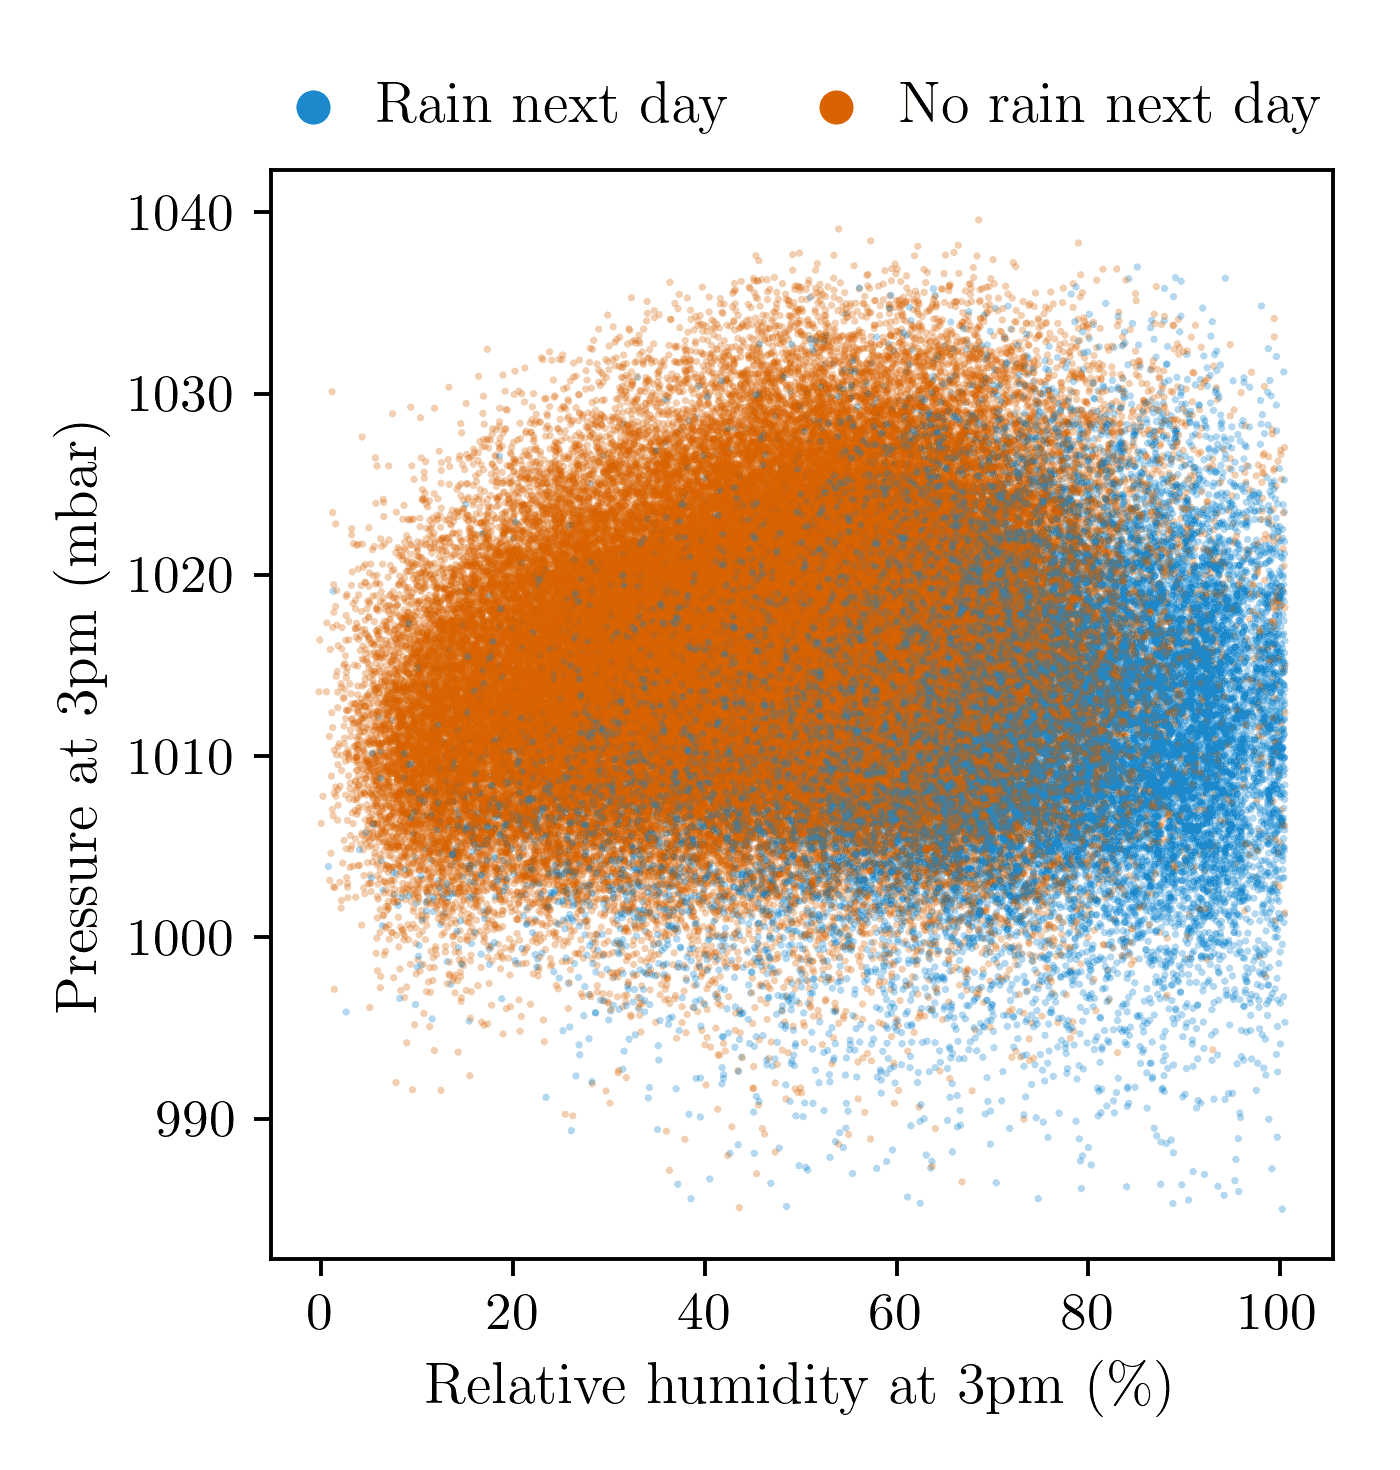
\includegraphics[scale=0.6]{graphics/weather_data.png}%
    \end{subfigure}
    \begin{subfigure}{0.49\textwidth}
      \centering
      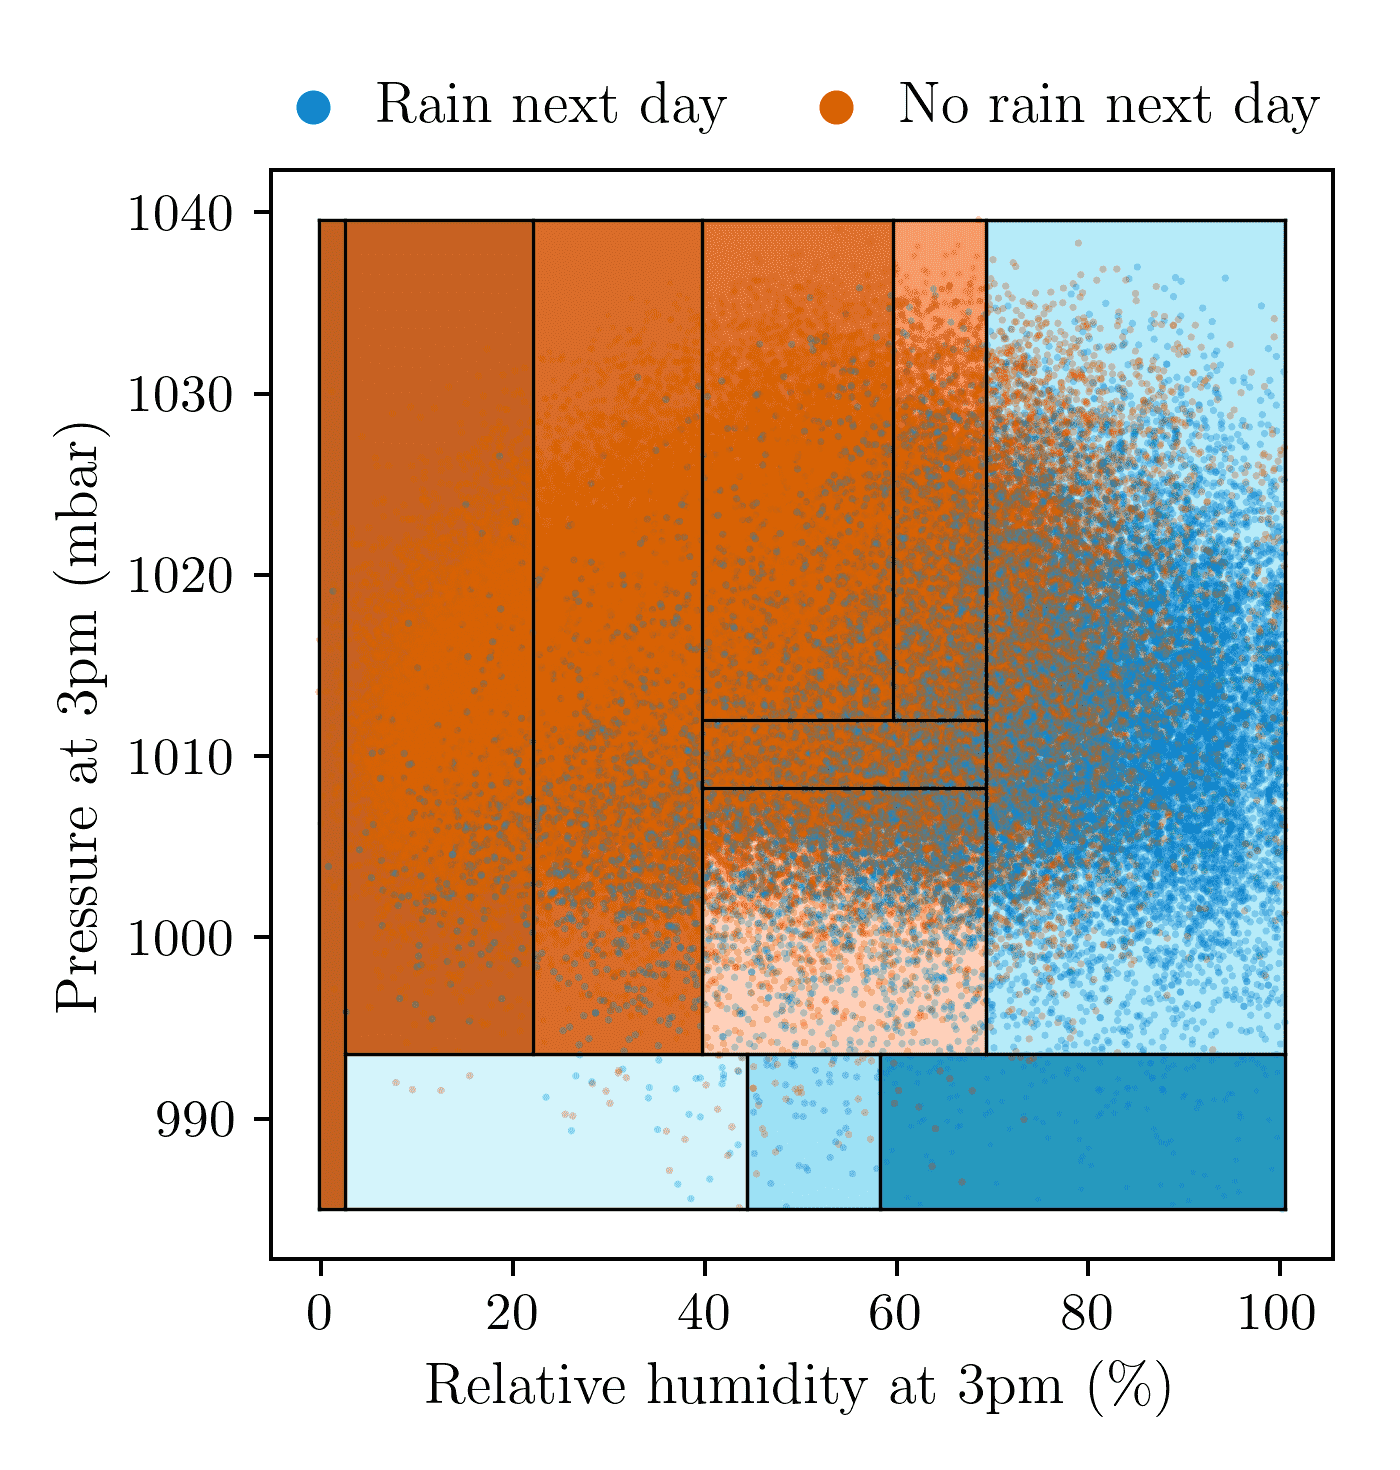
\includegraphics[scale=0.6]{graphics/weather_data_filled_partition.png}%
    \end{subfigure}
  \end{figure}

  \begin{figure}
    \centering
    \begin{subfigure}{0.49\textwidth}
      \centering
      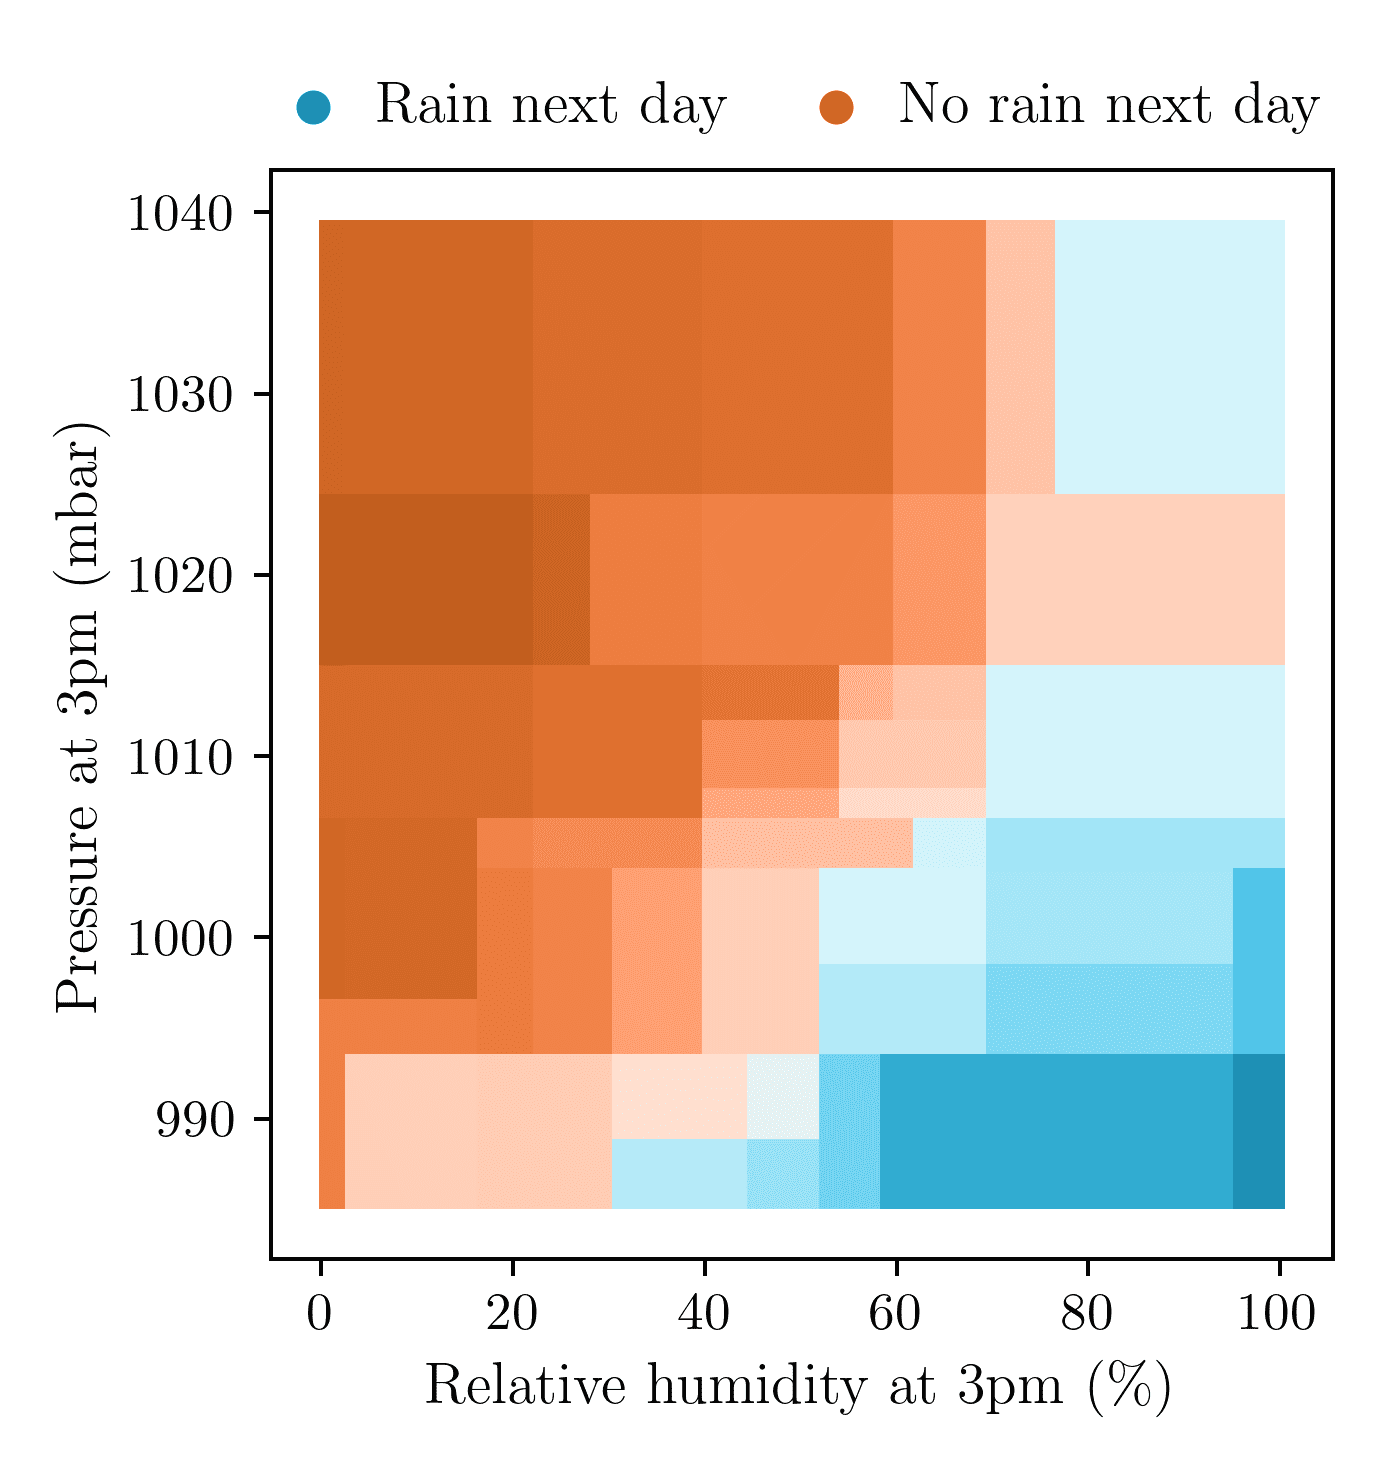
\includegraphics[scale=0.6]{graphics/weather_forest_2.png}%
    \end{subfigure}
    \begin{subfigure}{0.49\textwidth}
      \centering
      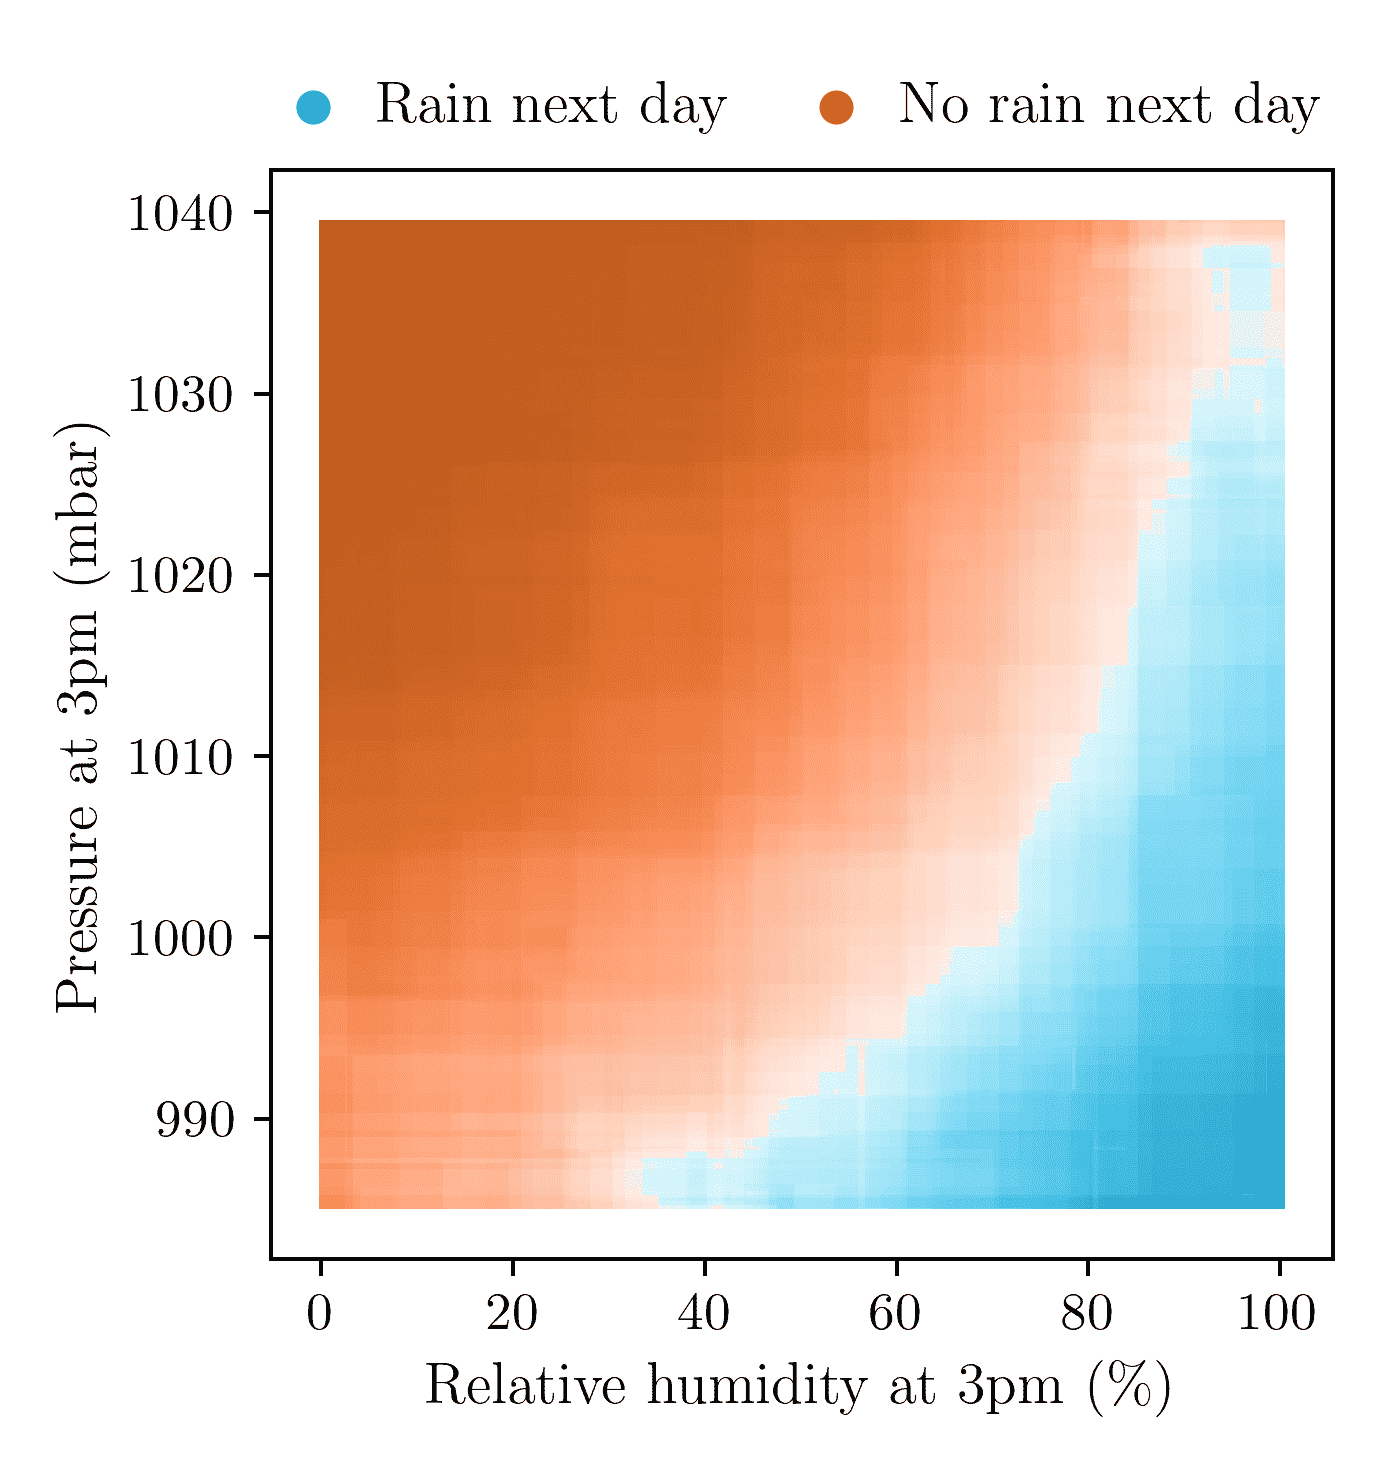
\includegraphics[scale=0.6]{graphics/weather_forest_30.png}%
    \end{subfigure}
  \end{figure}

  \begin{figure}
    \centering
    \begin{subfigure}{0.54\textwidth}
      \centering
      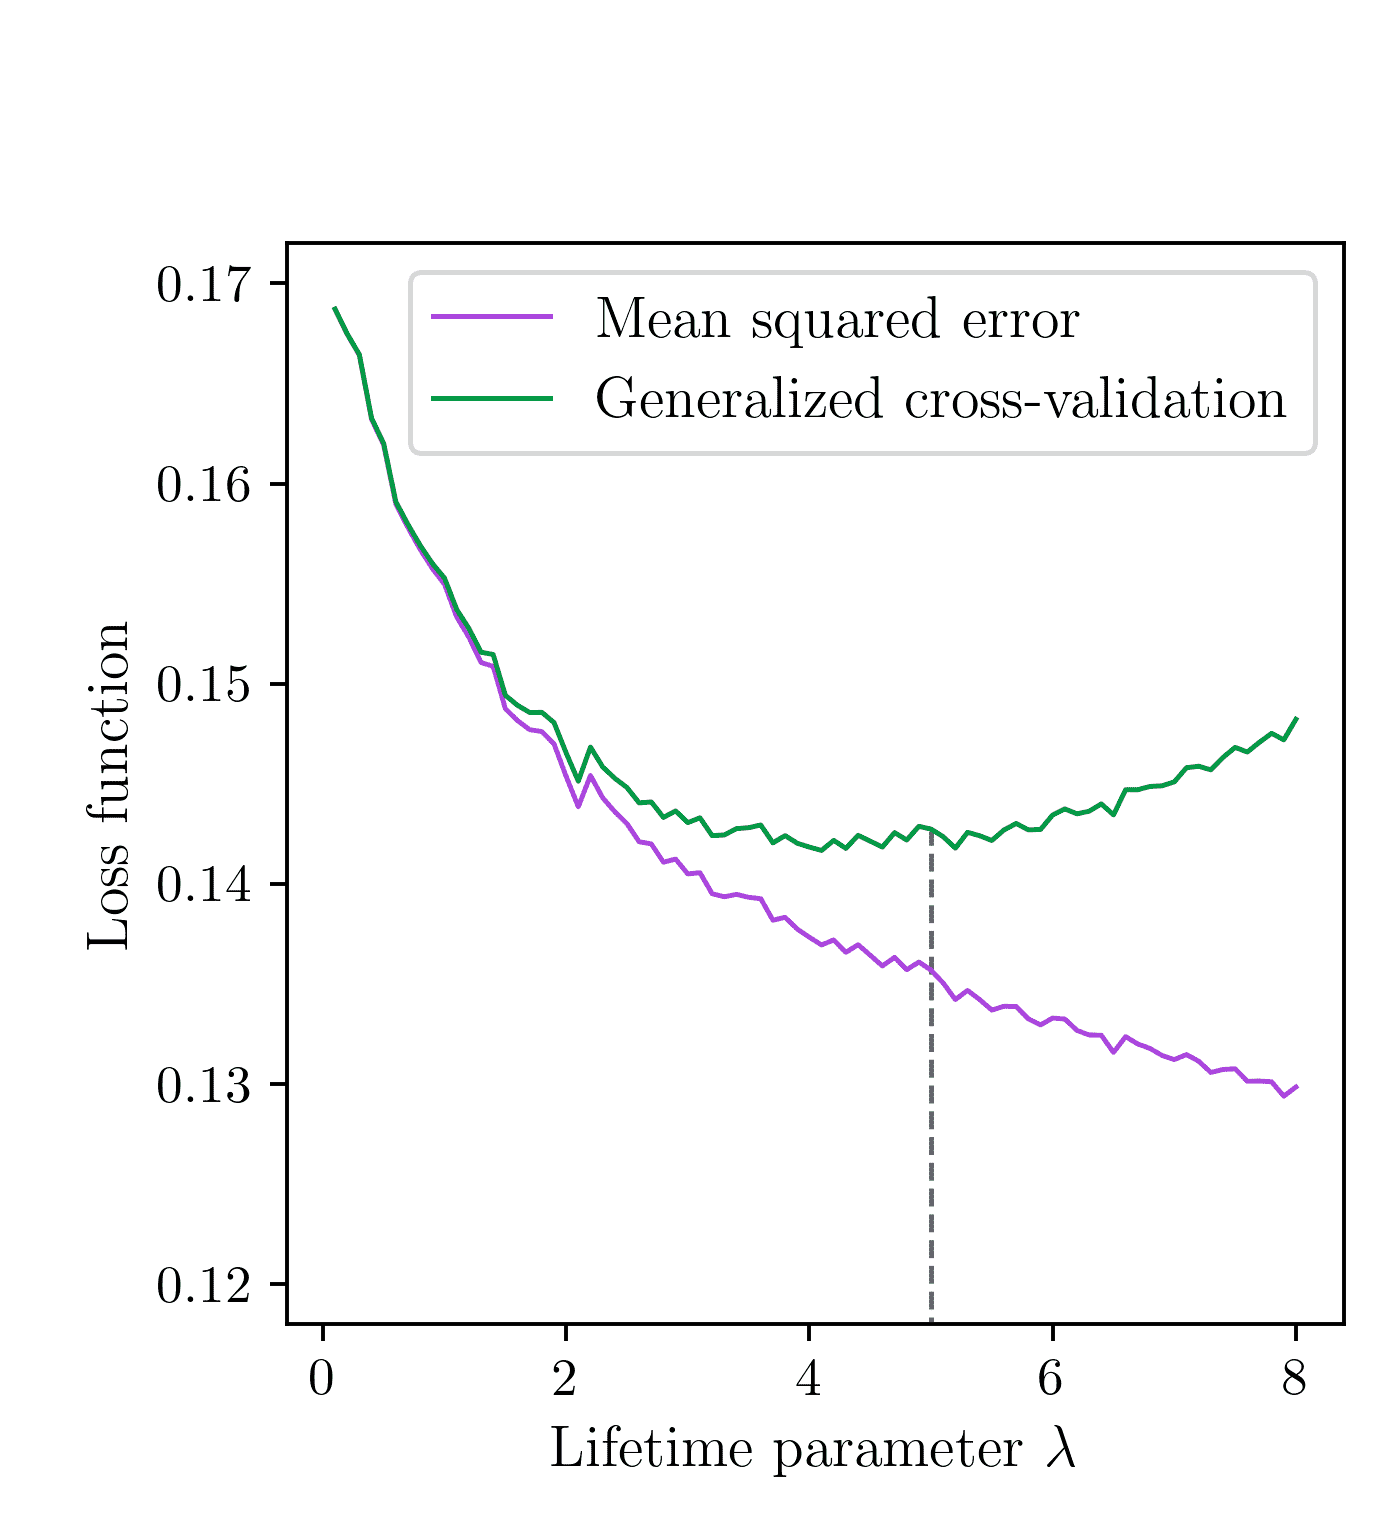
\includegraphics[scale=0.6]{graphics/weather_gcv.png}%
    \end{subfigure}
    \begin{subfigure}{0.45\textwidth}
      \centering
      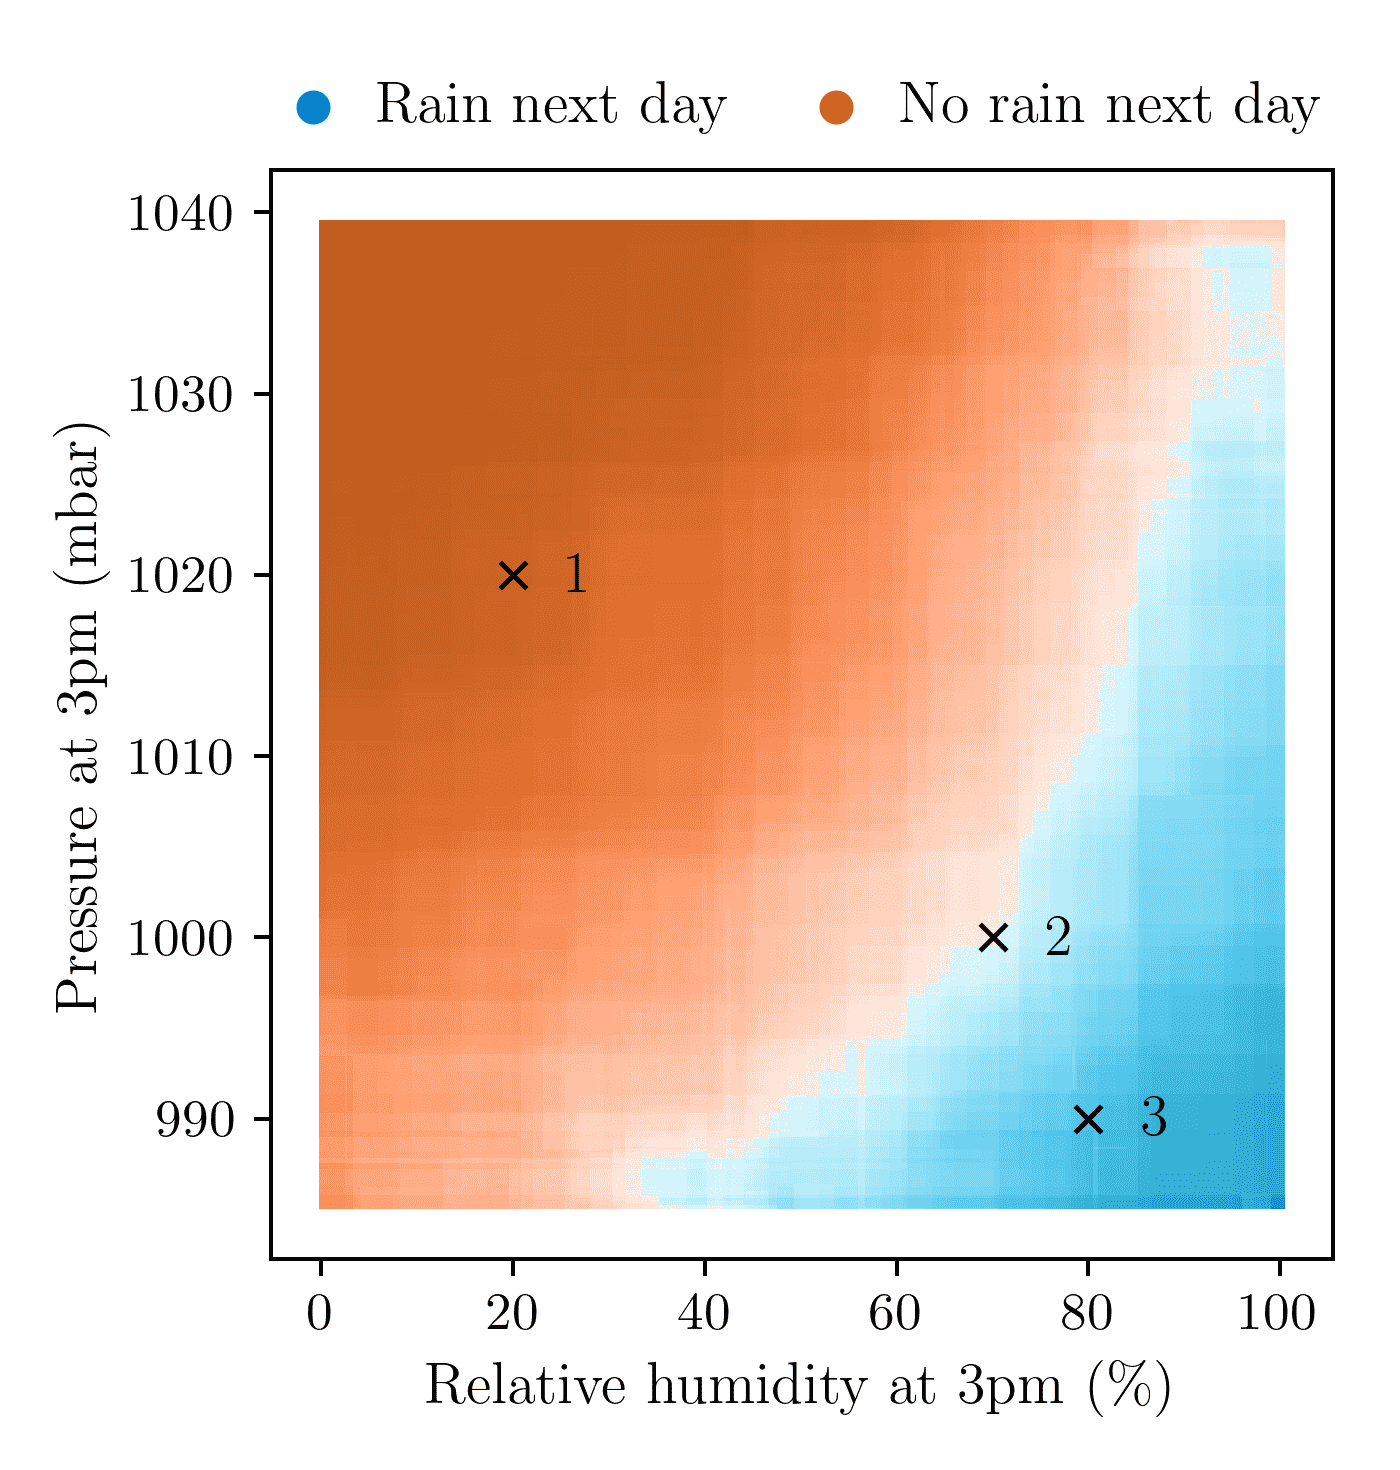
\includegraphics[scale=0.6]{graphics/weather_forest_design.png}%
    \end{subfigure}
  \end{figure}

\begin{table}
  \begin{center}
    \begin{tabular}{|c|c|r|c|c|}
      \hline
      \textbf{Point} & \textbf{Humidity} & \textbf{Pressure} &
      \textbf{Chance of rain} & \textbf{95\% confidence interval} \\
      \hline
      $1$ & $20\%$ & $1020\,\textrm{mbar}$ &
      $\phantom{0}4.3\%$ &
      \hspace*{-0mm}$4.1\%$ -- $4.6\%$ \\
      $2$ & $70\%$ & $1000\,\textrm{mbar}$ &
      $53.0\%$ &
      $52.0\%$ -- $54.0\%$ \\
      $3$ & $80\%$ & $990\,\textrm{mbar}$ &
      $77.5\%$ &
      $74.4\%$ -- $80.6\%$ \\
      \hline
    \end{tabular}
  \end{center}
\end{table}


\section{Conclusion}%
\label{sec:mondrian_conclusion}

We presented a central limit theorem for the Mondrian random forest
estimator and showed how it can be used to perform statistical inference
on an unknown nonparametric regression function.
We introduced a debiased version of Mondrian random forests, exploiting higher
order smoothness, and
demonstrated their advantages for statistical inference and their
minimax optimality properties.
Finally we discussed tuning parameter selection, enabling fully
feasible and practical estimation and inference procedures.
This work has been presented as
%
\cite{%
  underwood2024talkmichigan,%
  underwood2024talkillinois,%
  underwood2024talkpitt%
}.
